\UseRawInputEncoding
\documentclass[12pt, a4paper, oneside]{report}

% --- Core Academic Packages ---
\usepackage[utf8]{inputenc}
\usepackage{amsmath}      
\usepackage{amssymb}      
\usepackage{graphicx}     
\usepackage{subcaption} % For subfigure environment
\usepackage{geometry}     
\usepackage{booktabs}     
\usepackage{titlesec}     
\usepackage{fmtcount} % Converts numbers (1) into words (ONE)
\usepackage{etoolbox} % Allows us to patch styles dynamically
\usepackage{textcomp} % For \textohm (Ω symbol)
\usepackage{fancyhdr}
\usepackage{tocloft}
\usepackage{longtable}
\usepackage{array}
\pagestyle{fancy}
\fancyhf{}

\renewcommand{\chaptermark}[1]{%
  \markboth{#1}{}
}

\fancyhead[L]{\nouppercase{\leftmark}}
\fancyfoot[C]{\thepage}
\fancypagestyle{plain}{
    \fancyhf{}
    \fancyfoot[C]{\thepage}
    \renewcommand{\headrulewidth}{0pt}
}

\renewcommand{\headrulewidth}{0.4pt}

% --- Enforce Unified LaTeX Margins ---
\geometry{top=1in, bottom=1in, left=1.25in, right=1in}


% --- Define the Premium Full-Page Style for Actual Chapters ---
\newcommand{\applyFullPageChapterStyle}{%
  \titleformat{\chapter}[display]
    {\normalfont\centering} 
    {\vspace*{5cm}\Large\MakeUppercase{Chapter \NUMBERstring{chapter}}} 
    {4ex} 
    {\Huge\bfseries\centering\makebox[0pt]{\resizebox{2cm}{!}{\raisebox{1ex}{$\sim$}}} \\ \vspace{3ex}} 
    [\clearpage]
}

% --- Define the Normal Style for Index Pages ---
\newcommand{\applyNormalChapterStyle}{%
  \titleformat{\chapter}[display]
    {\normalfont\huge\bfseries}
    {\chaptername\ \thechapter}
    {20pt}
    {\Huge}
}
\usepackage{float} % Gives you the strict [H] force parameter
% --- Force Numbering and Contents Inclusion down to Level 3 (Subsubsections) ---
\setcounter{secnumdepth}{3} % Controls heading numbering depth
\setcounter{tocdepth}{3}    % Controls Table of Contents depth
\usepackage{tabularx}        % Enables self-wrapping, proportional columns
\usepackage[table]{xcolor}   % Enables the \rowcolors zebra striping command
% Forces \paragraph to break to a new line instead of staying inline
\titleformat{\paragraph}[hang]{\normalfont\normalsize\bfseries}{\theparagraph}{1em}{}
\usepackage{caption}

\captionsetup[table]{
    justification=raggedright,
    singlelinecheck=false,
    labelfont=bf,
    textfont=normalfont
}
\usepackage{listings}
\usepackage{xcolor}
\usepackage{siunitx}

% Custom MATLAB color palette
\definecolor{mgreen}{rgb}{0,0.6,0}
\definecolor{mgray}{rgb}{0.5,0.5,0.5}
\definecolor{mstring}{rgb}{0.62,0.12,0.94}
\definecolor{mbackground}{rgb}{0.98,0.98,0.98}

\lstset{
    language=Matlab,
    backgroundcolor=\color{mbackground},   
    commentstyle=\color{mgreen},
    keywordstyle=\color{blue},
    numberstyle=\tiny\color{mgray},
    stringstyle=\color{mstring},
    basicstyle=\ttfamily\small,
    breakatwhitespace=false,         
    breaklines=true,                 
    captionpos=b,                    
    keepspaces=true,                 
    numbers=left,                    
    numbersep=10pt,                  
    showspaces=false,                
    showstringspaces=false,
    showtabs=false,                  
    tabsize=4,
    frame=single,                     % Adds an elegant outer frame border
    rulecolor=\color{gray!30}
}
% ==========================================
% List of Figures Formatting
% ==========================================

% Show "Figure 1.1" instead of "1.1"
\renewcommand{\cftfigpresnum}{Figure~}
\renewcommand{\cftfigaftersnum}{\quad}
\setlength{\cftfignumwidth}{2.5cm}
\usepackage[hidelinks]{hyperref}
\begin{document}

% =========================================================================
% FRONT MATTER: Normal Index Styles
% =========================================================================
\begin{titlepage}
\thispagestyle{empty}

\begin{center}
\vspace*{1.5cm}
% Logo

\includegraphics[width=6cm]{Figures/logo.png} % غيري الاسم حسب اسم ملف اللوجو

\vspace{0.4cm}

{\small Electrical Power and Machines Department}

\vspace{0.5cm}

{\huge\bfseries Integration of Photovoltaic Systems and Energy Storage for Electric Vehicle Charging Station}

\vspace{0.3cm}

{\normalsize B.Sc. Graduation Project 2026}

\vspace{1.5cm}

{\large\textbf{Prepared by:}}

\vspace{0.3cm}

\begin{center}

\large

\renewcommand{\arraystretch}{1.4}

\begin{tabular}{c @{\hspace{2cm}} c}

\multicolumn{2}{c}{Nour El-Deen Mohamed Fathy} \\

\multicolumn{2}{c}{Abd El-Rahman Muhammad Saad} \\

\multicolumn{2}{c}{Hassan Ibrahim Hassan Al Halwani} \\

\multicolumn{2}{c}{Mai Nagah Ali} \\

\multicolumn{2}{c}{Mariam Mamdouh Ibrahim} \\

\multicolumn{2}{c}{Rewan Amr Mahmoud} \\

\multicolumn{2}{c}{Rwan Mohamed Abd-Elmokhtar} \\

\multicolumn{2}{c}{Yasmeen Salah Khobeez} \\

\multicolumn{2}{c}{Youssef Ebrahim Abd El-Sattar} \\

\end{tabular}

\end{center}

\vfill
{\Large Prof. Dr. Ahmed Abbas El Serougi}

\end{center}

\end{titlepage}
\pagenumbering{roman} 
\applyNormalChapterStyle % Forces Contents, Figures, and Tables to look normal

\tableofcontents
\clearpage

\listoffigures
\clearpage

\listoftables
\clearpage

\fancyhead[L]{List of Abbreviations} 

\fancypagestyle{plain}{
    \fancyhf{}
    \fancyfoot[C]{\thepage}         
    \renewcommand{\headrulewidth}{0pt}
}
\chapter*{List of Abbreviations}
\renewcommand{\arraystretch}{1.2}


\begin{longtable}{p{3cm}p{11cm}}

\textbf{Abbreviation} & \textbf{Definition} \\ \hline
\endfirsthead

\textbf{Abbreviation} & \textbf{Definition} \\ \hline
\endhead
CO2  & Carbon Dioxide \\
PV   & Photovoltaic \\
BOS  & Balance of System \\
STC  & Standard Test Conditions \\
DC   & Direct Current \\
AC   & Alternating Current \\
MPPT & Maximum Power Point Tracking \\
BESS  & Battery Energy Storage System \\
BMS  & Battery Management System \\
NiMH  & Nickel-Metal Hydride \\
Li-ion & Lithium-ion \\
EV   & Electric Vehicle \\
P\&O  & Perturb and Observe  \\
GMPPT & Global Maximum Power Point Tracking  \\
OBC  & On-Board Charger \\
PWM  & Pulse Width Modulation \\
SOC  & State of Charge \\
SPWM & Sinusoidal Pulse Width Modulation \\
THD  & Total Harmonic Distortion \\
Ir   & solar irradiance  \\
IBC  & Interleaved Boost Converter  \\
V2G  & Vehicle-to-Grid  \\
PI   & Proportional-Integral  \\
PLL  & Phase Locked Loop  \\
VSC  & Voltage Source Converter  \\
Id   & Direct current  \\
Iq   & Quadrature current  \\
BW   & BandWidth  \\
Ma   & Modulation Index  \\
CC   & Constant Current  \\
CV   & Constant Voltage  \\
PI   & Proportional-Integral  \\
PLL  & Phase Locked Loop  \\
VSC  & Voltage Source Converter  \\
Voc  & Open-Circuit Voltage  \\
Vmpp  & Voltage at Maximum Power  \\
Isc  & Short-Circuit Current  \\
Impp  & Current at Maximum Power \\
ESS  & Energy Storage System  \\
%last chapter 
DAB  & Dual Active Bridge  \\
ZVS  & Zero Voltage Switching  \\
WBG  & Wide-bandgap  \\
Si  & Silicon  \\
SiC  & Silicon Carbide  \\
GaN  & Gallium Nitride  \\
VB  & Valence Band  \\
CB  & Conduction Band  \\
AI  & Artificial Intelligence  \\
FLC  & Fuzzy Logic Control  \\
ANNs  & Artificial Neural Networks  \\
RL  & Reinforcement Learning  \\
EMS  & Energy Management System  \\
IoT  & Internet of Things  \\
ESS & Energy storage system \\
D & duty cycle  \\
$f_{s}$  & switching frequency  \\
$\Delta i_{l}$ & current ripples \\
% --- Added from Hardware Implementation (Section 6.2) ---
CCM & Continuous Conduction Mode \\
ESR & Equivalent Series Resistance \\
MCU & Microcontroller Unit \\
ADC & Analog-to-Digital Converter \\
ISR & Interrupt Service Routine \\
DSO & Digital Storage Oscilloscope \\
$R_{DS(on)}$ & On-State Drain-to-Source Resistance \\
$V_{DS}$ & Drain-to-Source Breakdown Voltage \\
$C_{iss}$ & Input Capacitance \\
$Q_{gd}$ & Gate-to-Drain Miller Charge \\
$T_J$ & Junction Temperature \\
$T_C$ & Case Temperature \\
CTR & Current Transfer Ratio \\
OVP & Over-Voltage Protection \\
UVP & Under-Voltage Protection \\
OCP & Over-Current Protection \\
UVLO & Under-Voltage Lockout \\
SGND & Signal Ground \\
PGND & Power Ground \\
\end{longtable}

\clearpage

\fancyhead[L]{\nouppercase{\leftmark}} 
\fancypagestyle{plain}{
    \fancyhf{}
    \fancyfoot[C]{\thepage}          
    \renewcommand{\headrulewidth}{0pt} 
}

% =========================================================================
% MAIN TEXT: Switch to Premium Full-Page Style for Chapters
% =========================================================================
\pagenumbering{arabic} 
\applyFullPageChapterStyle % Switches style to full-page text with flourish right here
\chapter{Introduction}
% =========================================================================
% CHAPTER 1: INTRODUCTION
% =========================================================================


\section{Background}
Energy is one of the fundamental pillars of modern society, driving economic growth, industrial development, technological advancement, and improving the quality of life. With the continuous growth of the global population and the rapid expansion of industrialization and urbanization, the demand for electricity has increased significantly in the past several decades. This growing demand has created major challenges in ensuring a reliable, sustainable, and environmentally friendly energy supply.

Traditionally, electricity generation has relied heavily on conventional energy resources such as coal, petroleum, and natural gas. Although fossil fuels have long been the primary source of global electricity generation, their extensive use has resulted in serious environmental challenges. The combustion of fossil fuels releases greenhouse gasses, particularly carbon dioxide (CO2), contributing to global warming, climate change, and air pollution.
In addition, fossil fuel reserves are finite, raising concerns about future energy security.

To address these challenges, the global energy sector has increasingly shifted toward renewable energy resources, which provide clean and sustainable alternatives to conventional energy sources. Consequently, governments, researchers, and industries have invested significant efforts in developing renewable energy technologies and integrating them into
modern electrical power systems.

Among the various renewable energy resources, solar energy has emerged as one of the most promising solutions due to its abundance, accessibility, and minimal environmental impact. The development of photovoltaic (PV) technology has enabled the direct conversion of solar radiation into electrical energy without harmful emissions during operation.
Continuous improvements in photovoltaic materials and manufacturing technologies have enhanced system efficiency while reducing installation costs, making PV systems suitable for residential, commercial, industrial, and utility-scale applications. Today, photovoltaic systems are among the fastest-growing renewable energy technologies worldwide. Their widespread deployment is expected to play a vital role in achieving sustainable development goals, reducing dependence on fossil fuels, and meeting
the growing global demand for clean, reliable, and sustainable electrical energy\cite{masters2013}.

\section{Problem Statement}
The continuous increase in electricity demand has placed considerable pressure on existing power generation systems. Conventional energy resources, which have been the dominant source of electricity production for decades, are associated with several challenges, including limited availability, fluctuating fuel prices, greenhouse gas emissions, and environmental degradation. These issues have raised concerns regarding the ability of current energy systems to satisfy future energy demands in a sustainable manner.

Moreover, many regions around the world continue to experience difficulties in providing reliable electricity due to increasing consumption, population growth, and the depletion of non-renewable energy resources. These challenges highlight the necessity of adopting cleaner, more efficient, and sustainable energy generation technologies that can reduce environmental impacts while maintaining energy security.

Therefore, it has become essential to investigate modern energy solutions capable of meeting the growing electricity demand while minimizing dependence on conventional energy resources. This study contributes to this objective by exploring one of the most promising technologies for sustainable electricity generation.


\section{Renewable Energy}
Renewable energy has become an essential component of modern power systems due to its ability to provide clean and sustainable energy while reducing the environmental impacts associated with conventional energy resources. The increasing global demand for electricity, together with growing concerns about climate change and energy security, has accelerated the development and deployment of renewable energy technologies. Today, renewable energy is widely utilized in residential, commercial, industrial, and utility-scale applications, contributing significantly to the transition toward a more sustainable energy sector.

\subsection{Definition of Renewable Energy}
Renewable energy is defined as energy derived from natural resources that are continuously replenished through natural processes. Unlike fossil fuels, which require millions of years to form and exist in finite quantities, renewable resources are naturally regenerated and can provide a continuous supply of energy when properly utilized. The primary renewable energy resources include solar energy, wind energy, hydropower, biomass, and geothermal energy.

These resources are converted into electrical or thermal energy using different energy conversion technologies. For instance, photovoltaic systems convert solar radiation directly into electricity, while wind turbines convert the kinetic energy of moving air into electrical power. Similarly, hydropower plants utilize the potential and kinetic energy of flowing water to drive turbines connected to electrical generators.


\subsection{Importance of Renewable Energy}
Renewable energy plays a crucial role in addressing many of the challenges facing modern energy systems. It contributes to reducing greenhouse gas emissions, improving air quality, and decreasing dependence on conventional fossil fuels. Furthermore, renewable energy enhances energy security by utilizing locally available natural resources, thereby reducing the need for imported fuels and increasing the stability of national energy supplies.
In addition to its environmental and economic benefits, renewable energy supports sustainable development by promoting technological innovation, creating employment opportunities, and expanding access to electricity, particularly in remote and rural regions.


\begin{figure}[H]
    \centering
    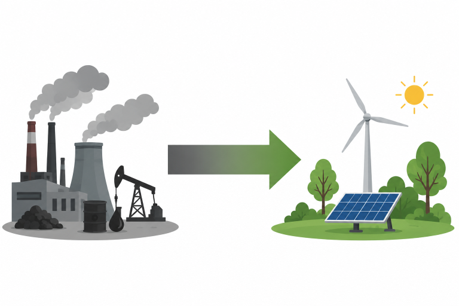
\includegraphics[width=0.75\textwidth]{Figures/Figure 1.1.png}
    \caption{Transition from conventional energy systems to renewable energy systems.}
    \label{fig:energy_transition}
\end{figure}

\subsection{Benefits of Renewable Energy}
Renewable energy provides numerous advantages that make it an attractive alternative to conventional energy resources. It significantly reduces carbon emissions during electricity generation, minimizes environmental pollution, and relies on naturally replenished resources. Moreover, renewable energy systems require relatively low operating and maintenance costs after installation and contribute to improving the diversity and reliability of electrical power systems.

\subsection{Limitations of Renewable Energy}
Despite its numerous advantages, renewable energy technologies still face several technical and economic challenges. The availability of renewable resources often depends on weather conditions and geographical location, resulting in intermittent power generation. Furthermore, the integration of renewable energy into electrical grids requires advanced energy storage technologies, intelligent control systems, and substantial initial investments to ensure reliable and continuous electricity supply.

\section{Renewable Energy Sources}
Renewable energy can be harnessed from various natural resources that are continuously replenished through natural processes. These resources differ in terms of availability, energy conversion methods, efficiency, and practical applications. However, they all share the common objective of providing sustainable energy while reducing dependence on conventional fossil fuels. The primary renewable energy resources include solar energy, wind energy, hydropower, biomass energy, and geothermal energy, each contributing to the diversification of the global energy portfolio.

\begin{figure}[H]
    \centering
    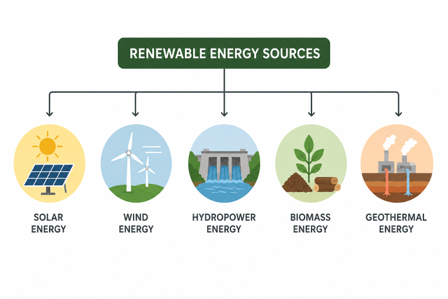
\includegraphics[width=0.75\textwidth]{Figures/Figure 1.2.png}
    \caption{Classification of renewable energy sources.}
    \label{fig:renewable_classification}
\end{figure}

\subsection{Solar Energy}
Solar energy is the energy obtained from solar radiation emitted by the sun. It is considered one of the most abundant and widely available renewable energy resources and can be converted into electrical or thermal energy using different technologies. Owing to its widespread availability and continuous technological development, solar energy has become one of the fastest-growing renewable energy resources worldwide.

\subsection{Wind Energy}
Wind energy utilizes the kinetic energy of moving air to generate electricity through wind turbines. It is a clean and sustainable source of energy that is widely implemented in regions with favorable wind conditions, particularly in coastal and open-land areas.

\subsection{Hydropower}
Hydropower converts the potential and kinetic energy of flowing or falling water into electrical energy using hydraulic turbines. It is one of the oldest and most established renewable energy technologies and is widely used for large-scale electricity generation.

\subsection{Biomass Energy}
Biomass energy is produced from organic materials such as agricultural residues, forestry waste, and other biodegradable resources. These materials can be converted into electricity, heat, or bio-fuels through various biological and thermochemical processes.

\subsection{Geothermal Energy}
Geothermal energy utilizes the thermal energy stored beneath the Earth’s surface for electricity generation and heating applications. It provides a stable and reliable source of energy in regions with suitable geothermal resources.

\section{Solar Energy}
Although several renewable energy resources are available for electricity generation, solar energy has emerged as one of the most promising and widely adopted energy sources due to its abundance, sustainability, and continuous technological advancements. Solar radiation is available in most regions of the world and can be efficiently converted into useful energy using modern conversion technologies.

In particular, countries located within the global sunbelt region, including Egypt, receive high levels of solar irradiance throughout the year, making solar energy an attractive option for electricity generation. As a result, solar energy has become a fundamental component of modern sustainable energy systems and has found extensive applications in residential, commercial, industrial, and transportation sectors.

\subsection{Solar Radiation}
Solar radiation is the electromagnetic energy emitted by the sun as a result of continuous nuclear fusion reactions occurring within its core. This energy propagates through space and reaches the Earth’s atmosphere, where a portion is reflected back into space, another portion is absorbed by atmospheric gases and clouds, while the remaining radiation reaches the Earth’s surface and becomes available for energy conversion.

The amount of solar radiation received at a specific location depends on several factors, including geographical latitude, season of the year, atmospheric conditions, and time of day. Consequently, solar energy availability varies from one region to another, directly influencing the performance of solar energy systems.

Solar radiation reaching the Earth’s surface is generally classified into three main components: direct radiation, diffuse radiation, and reflected radiation. Direct radiation reaches the Earth’s surface without atmospheric scattering, diffuse radiation is scattered by molecules and particles within the atmosphere, whereas reflected radiation originates from sunlight reflected by surrounding objects and the ground. The combination of these components is referred to as global solar radiation, which represents the total solar energy available for solar energy conversion systems.


\begin{figure}[H]
    \centering
    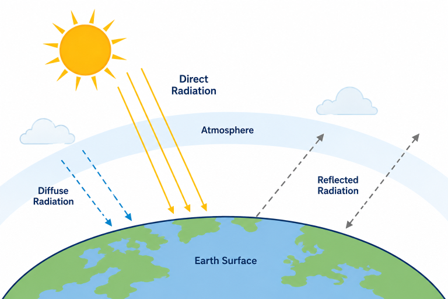
\includegraphics[width=0.75\textwidth]{Figures/Figure 1.3.png}
    \caption{Solar radiation reaching the Earth’s surface.}
    \label{fig:solar_radiation}
\end{figure}


\subsection{Applications of Solar Energy}
The unique characteristics of solar energy have enabled its utilization in a wide range of applications across residential, commercial, industrial, and agricultural sectors. Depending on the required form of energy, solar energy can be employed to provide electricity, heating, and power for remote locations where access to conventional energy sources is limited.

One of the most common applications of solar energy is electricity generation for residential and commercial buildings, where it contributes to reducing dependence on conventional power grids and lowering greenhouse gas emissions. Solar energy is also widely utilized for street lighting, water pumping and irrigation systems, telecommunication stations, and rural electrification projects, providing reliable energy in isolated areas.

In addition, the rapid growth of the transportation sector has created new opportunities for solar energy utilization. The increasing adoption of electric vehicles has encouraged the development of solar-powered charging solutions, supporting the transition toward sustainable transportation while reducing dependence on fossil fuels. As a result, solar energy has become an essential component of modern clean energy systems.


\begin{figure}[H]
    \centering
    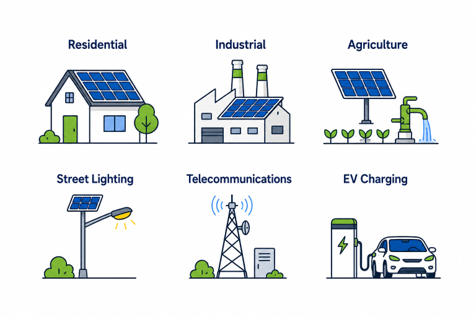
\includegraphics[width=0.75\textwidth]{Figures/Figure 1.4.png}
    \caption{Various applications of solar energy.}
    \label{fig:solar_applications}
\end{figure}

\subsection{Advantages and Challenges of Solar Energy}
Solar energy has become one of the most attractive renewable energy resources due to its environmental, economic, and technical benefits. It is an abundant and inexhaustible source of energy that is naturally replenished and available in most regions of the world. During operation, solar energy systems produce electricity without emitting greenhouse gases or air pollutants, contributing to environmental protection and climate change mitigation. In addition, solar energy systems generally require low operating and maintenance costs and can be deployed at various scales, ranging from small residential installations to large utility-scale power plants.

Despite these advantages, several challenges still limit the widespread utilization of solar energy. The amount of energy generated depends on solar irradiance, which varies according to weather conditions, seasonal changes, and the time of day. Consequently, electricity generation is intermittent and unavailable during nighttime. Moreover, the relatively high initial installation cost and the need for efficient energy storage technologies remain important considerations in solar energy systems. Continuous technological developments are therefore focused on improving system efficiency, reducing installation costs, and enhancing the reliability of solar energy utilization.


\section{Photovoltaic Systems}
Although solar energy is an abundant and sustainable source of renewable energy, it must be converted into electrical energy before it can be utilized in most practical applications. This conversion is achieved using photovoltaic (PV) technology, which directly transforms solar radiation into electricity through semiconductor materials. Owing to its high efficiency, reliability, and environmental benefits, photovoltaic technology has become one of the fastest-growing electricity generation technologies worldwide and plays a fundamental role in modern renewable energy systems.

\subsection{History and Development of Photovoltaic Technology}
The history of photovoltaic (PV) technology began in 1839 when the French physicist Alexandre Edmond Becquerel discovered the photovoltaic effect while conducting experiments on metal electrodes immersed in an electrolyte solution exposed to sunlight. His discovery demonstrated, for the first time, that light energy could be directly converted into electrical energy, laying the scientific foundation for modern photovoltaic technology.

The first practical attempt to utilize this phenomenon was made in 1883 by the American inventor Charles Fritts, who developed the first selenium-based solar cell. Although its energy conversion efficiency was relatively low, this achievement represented the first successful implementation of photovoltaic energy conversion and marked an important milestone in the evolution of solar cell technology.

A major breakthrough was achieved in 1954 when researchers at Bell Laboratories developed the first practical silicon solar cell with significantly higher conversion efficiency, making photovoltaic technology suitable for real-world applications. A few years later, in 1958, photovoltaic cells were successfully employed to power the Vanguard 1 satellite, demonstrating their exceptional reliability and establishing photovoltaics as a preferred energy source for space applications.

Since then, continuous advancements in semiconductor materials, manufacturing techniques, and power electronic technologies have significantly improved the efficiency, durability, and cost-effectiveness of photovoltaic systems. These developments have enabled the widespread deployment of PV systems in residential, commercial, industrial, and utility-scale electricity generation. Today, photovoltaic technology has become one of the leading renewable energy technologies for clean and sustainable electricity production worldwide.


\begin{figure}[H]
    \centering
    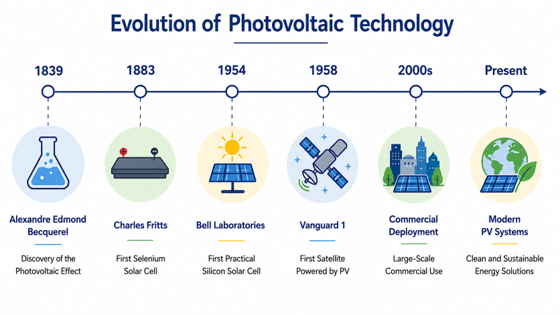
\includegraphics[width=0.85\textwidth]{Figures/Figure 1.5.png}
    \caption{Major milestones in the development of photovoltaic technology.}
    \label{fig:pv_history}
\end{figure}

\newpage

\subsection{Photovoltaic System Components}
Photovoltaic (PV) systems consist of several interconnected components that work together to convert solar energy into usable electrical power. The basic building block of every photovoltaic system is the photovoltaic cell, which converts sunlight directly into electricity through the photovoltaic effect. To satisfy practical power requirements, individual cells are electrically interconnected to form modules, while multiple modules are combined into arrays capable of generating higher voltage and power levels. In addition to the photovoltaic array, a complete PV system includes several auxiliary components, collectively referred to as the Balance of System (BOS), which ensure efficient energy conversion, control, protection, and power delivery.

\subsubsection{Photovoltaic Cell}
A photovoltaic (PV) cell is the fundamental building block of every photovoltaic system and is the smallest unit capable of directly converting solar energy into electrical energy through the photovoltaic effect. It is typically fabricated from semiconductor materials, with crystalline silicon being the most widely used due to its high efficiency, reliability, and long operational lifetime. A single photovoltaic cell generates a relatively small electrical output, typically around 0.5–0.7 V under standard test conditions (STC), making it necessary to electrically connect multiple cells to obtain practical voltage and power levels.

\begin{figure}[H]
    \centering
    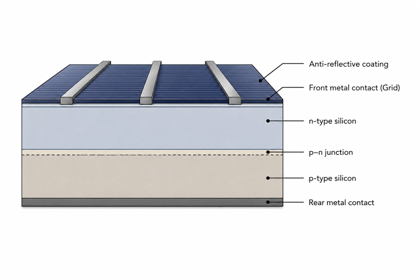
\includegraphics[width=0.65\textwidth]{Figures/Figure 1.6.png}
    \caption{Cross-sectional structure of a photovoltaic cell.}
    \label{fig:pv_cell_structure}
\end{figure}

The structure of a photovoltaic cell is carefully designed to maximize sunlight absorption while minimizing electrical losses. The front surface is covered with an anti-reflective coating to reduce optical reflection and increase the amount of incident solar radiation entering the semiconductor. Metallic contacts are provided on both the front and rear surfaces to collect the generated charge carriers and transfer the electrical current to the external circuit. These structural components enable efficient energy conversion and provide the foundation for larger photovoltaic modules and arrays.

\subsubsection{Photovoltaic Module}
Since the electrical output of a single photovoltaic cell is relatively low, multiple photovoltaic cells are electrically interconnected to form a photovoltaic module. The cells are typically connected in series to increase the output voltage, while parallel connections are used when higher current is required. The interconnected cells are encapsulated between protective layers, including tempered glass, polymer encapsulant materials, and a durable backsheet, to provide mechanical strength and protect the cells from environmental conditions such as moisture, dust, and temperature variations.

\begin{figure}[H]
    \centering
    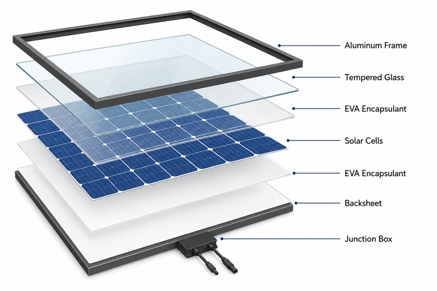
\includegraphics[width=0.65\textwidth]{Figures/Figure 1.7.png}
    \caption{Exploded view of a photovoltaic module showing its main structural components.}
    \label{fig:pv_module_exploded}
\end{figure}

Photovoltaic modules are manufactured in standardized sizes and power ratings to facilitate system design and installation. Depending on the application, modules can be connected together in various electrical configurations to achieve the required voltage, current, and power output. As the primary structural unit of a photovoltaic array, modules provide a practical balance between electrical performance, mechanical durability, and ease of maintenance.

\subsubsection{Photovoltaic Array}
A photovoltaic array consists of multiple photovoltaic modules electrically interconnected to provide the voltage, current, and power required for a specific application. The modules may be connected in series to increase the output voltage or in parallel to increase the output current. In practical PV installations, a combination of series and parallel connections is commonly employed to achieve the desired electrical characteristics while meeting the system’s power demand.

The electrical output of a photovoltaic array depends on several operating conditions, including solar irradiance, cell temperature, shading, and the electrical configuration of the modules. By adjusting the number of modules connected in series and parallel, PV arrays can be designed to satisfy a wide range of residential, commercial, and industrial energy requirements. Consequently, the photovoltaic array represents the primary power-generating unit within a photovoltaic system.

\begin{figure}[H]
    \centering
    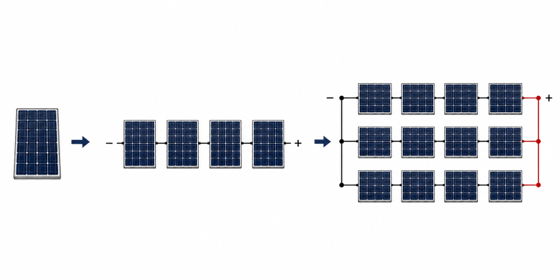
\includegraphics[width=0.75\textwidth]{Figures/Figure 1.8.png}
    \caption{Formation of a photovoltaic array from modules connected in series and parallel.}
    \label{fig:pv_array_formation}
\end{figure}


\subsubsection{Balance of System (BOS)}
In addition to photovoltaic modules and arrays, a complete photovoltaic system requires several auxiliary components collectively known as the Balance of System (BOS). These components are responsible for controlling, protecting, converting, storing, and delivering the generated electrical energy. Although they do not directly generate electricity, BOS components play a crucial role in ensuring the safe, reliable, and efficient operation of the entire photovoltaic system.

\subsection{Operating Principle of Photovoltaic Systems}
The operation of a photovoltaic (PV) system begins when solar radiation reaches the surface of a photovoltaic cell. Sunlight consists of tiny packets of energy known as photons. As these photons strike the surface of the PV cell, a portion of their energy penetrates the semiconductor material, initiating the energy conversion process. The amount of absorbed solar energy depends on the intensity of solar irradiance and the optical properties of the photovoltaic material.

\begin{figure}[H]
    \centering
    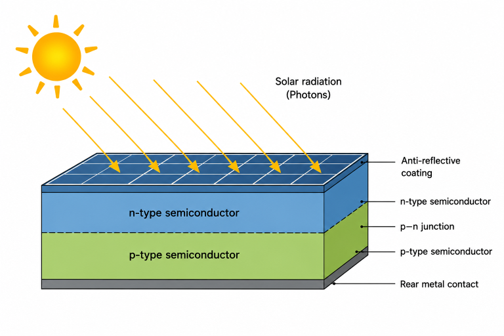
\includegraphics[width=0.55\textwidth]{Figures/Figure 1.9.png}
    \caption{Incident solar radiation on a photovoltaic cell.}
    \label{fig:pv_incident}
\end{figure}

\newpage

When photons penetrate the semiconductor material, they transfer their energy to the electrons bound within the silicon atoms. If the energy of an incident photon is equal to or greater than the band-gap energy of the semiconductor, the electron gains sufficient energy to break free from its atomic bond and move into the conduction band. Consequently, an empty position, known as a hole, is left behind in the valence band. The simultaneous creation of a free electron and a hole is referred to as an electron–hole pair, representing the first step in the generation of electrical energy within a photovoltaic cell.

\begin{figure}[H]
    \centering
    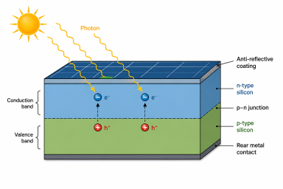
\includegraphics[width=0.55\textwidth]{Figures/Figure 1.10.png}
    \caption{Generation of electron–hole pairs inside a photovoltaic cell.}
    \label{fig:pv_eh_pairs}
\end{figure}

The electron–hole pairs generated within the photovoltaic cell are immediately separated by the built-in electric field established across the p–n junction. This electric field drives the free electrons toward the n-type semiconductor layer, while the holes move toward the p-type layer. By separating the charge carriers, the electric field minimizes their recombination and creates a potential difference across the cell, which is essential for generating electrical power.

\begin{figure}[H]
    \centering
    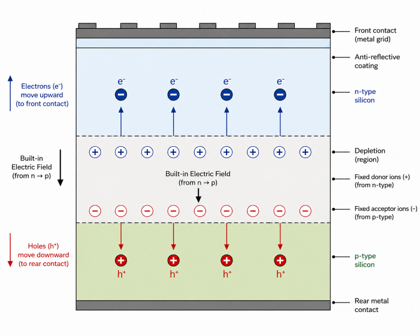
\includegraphics[width=0.55\textwidth]{Figures/Figure 1.11.png}
    \caption{Separation of charge carriers by the built-in electric field.}
    \label{fig:pv_separation}
\end{figure}

\newpage

When an external electrical circuit is connected to the photovoltaic cell, the separated electrons flow through the external circuit from the n-type contact to the p-type contact, producing a direct current (DC). As the electrons pass through the connected electrical load, they deliver useful electrical energy before returning to the photovoltaic cell, where the cycle continues as long as sunlight is available.

\begin{figure}[H]
    \centering
    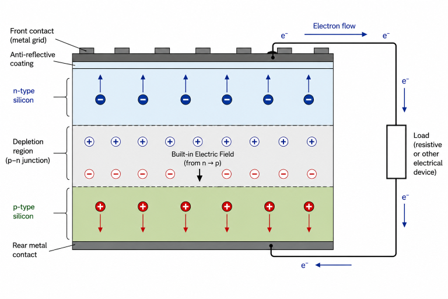
\includegraphics[width=0.55\textwidth]{Figures/Figure 1.12.png}
    \caption{Electron flow through the external circuit producing direct current (DC).}
    \label{fig:pv_current_flow}
\end{figure}

\subsection{Photovoltaic System Configurations}
Photovoltaic systems can be configured using different electrical architectures depending on the required power capacity, system efficiency, reliability, and application requirements. The configuration of a PV system determines how photovoltaic modules are interconnected and how the generated electrical power is processed before being supplied to the load or the utility grid. Among the most common configurations are centralized, string, and multi-string photovoltaic systems, each offering distinct advantages and limitations in terms of performance, flexibility, maintenance, and energy conversion efficiency.

\subsubsection{Centralized Photovoltaic Configuration}
In a centralized photovoltaic configuration, multiple photovoltaic strings are connected to a single central power conversion unit equipped with a common maximum power point tracking (MPPT) controller. This architecture is widely employed in large-scale photovoltaic power plants because of its simple design, reduced installation cost, and ease of implementation. However, since all PV strings operate under a single MPPT controller, the overall system performance can be significantly affected by partial shading, module mismatch, or faults occurring within individual strings. As a result, the entire system operates according to a common operating point rather than the optimum operating point of each individual string, leading to a reduction in the overall energy yield.

\begin{figure}[H]
    \centering
    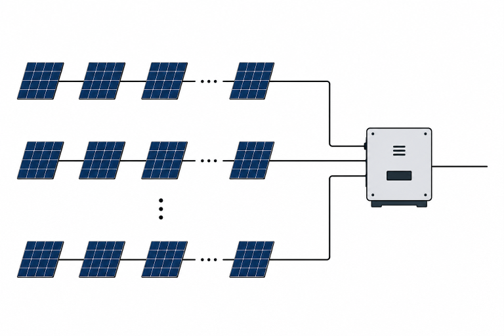
\includegraphics[width=0.65\textwidth]{Figures/Figure 1.13.png}
    \caption{Conceptual illustration of a centralized photovoltaic system configuration.}
    \label{fig:central_config}
\end{figure}

\subsubsection{String Photovoltaic Configuration}
In a string photovoltaic configuration, each photovoltaic string is connected to its own power conversion unit equipped with an independent maximum power point tracking (MPPT) controller. This allows every string to operate independently at its individual maximum power point, thereby improving the overall energy harvest under non-uniform operating conditions. Compared with the centralized configuration, this architecture significantly reduces the impact of partial shading, module mismatch, and string faults on the overall system performance. Consequently, string photovoltaic systems offer higher flexibility, improved reliability, and easier maintenance, making them widely adopted in residential and commercial photovoltaic installations.

\begin{figure}[H]
    \centering
    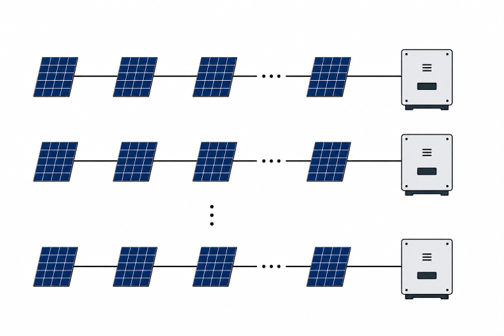
\includegraphics[width=0.65\textwidth]{Figures/Figure 1.14.png}
    \caption{Conceptual illustration of a string photovoltaic system configuration.}
    \label{fig:string_config}
\end{figure}

\newpage

\subsubsection{Multi-String Photovoltaic Configuration}
A multi-string photovoltaic configuration combines the advantages of both centralized and string photovoltaic systems. In this architecture, each photovoltaic string is connected to an individual DC–DC converter equipped with an independent maximum power point tracking (MPPT) controller before being connected to a common DC bus.

This enables each string to operate at its own maximum power point regardless of the operating conditions of the other strings, thereby maximizing the overall energy harvested from the photovoltaic array.
Comparison of the main characteristics of centralized, string, and multi-string photovoltaic system configurations.


\begin{figure}[H]
    \centering
    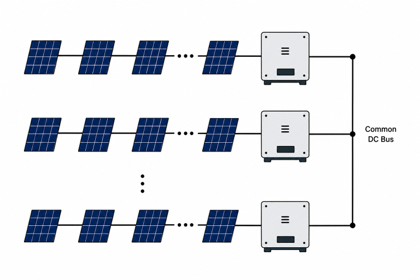
\includegraphics[width=0.65\textwidth]{Figures/Figure 1.15.png}
    \caption{Conceptual illustration of a multi-string photovoltaic system configuration.}
    \label{fig:multistring_config}
\end{figure}

\begin{table}[H]
    \centering
    \caption{Comparison of the main characteristics of centralized, string, and multi-string photovoltaic system configurations.}
    \label{tab:pv_configurations}
    \smallskip
    \smallskip
    \renewcommand{\arraystretch}{1.4} % Nice breathing room between rows
    \rowcolors{2}{white}{gray!8} % Clean alternating zebra stripes
    
    % This customizes the width ratios of your columns perfectly
    \begin{tabularx}{\textwidth}{
        >{\hsize=1.4\hsize\raggedright\arraybackslash}X 
        >{\hsize=0.86\hsize\raggedright\arraybackslash}X 
        >{\hsize=0.86\hsize\raggedright\arraybackslash}X 
        >{\hsize=0.88\hsize\raggedright\arraybackslash}X
    }
        \toprule
        \textbf{Feature} & \textbf{Centralized} & \textbf{String} & \textbf{Multi-String} \\
        \midrule
        Number of MPPT Controllers & One & One per String & One per String \\
        MPPT Operation & Common MPPT & Independent MPPT & Independent MPPT \\
        Power Conversion Architecture & Single Central Converter & One Converter per String & One Converter per String + Common DC Bus \\
        Common DC Bus & No & No & Yes \\
        Partial Shading Performance & Poor & Good & Excellent \\
        Module Mismatch Tolerance & Low & High & Very High \\
        System Reliability & Moderate & High & Very High \\
        Scalability & Limited & Good & Excellent \\
        Maintenance & Difficult & Easy & Easy \\
        Initial Cost & Low & Moderate & Higher \\
        \bottomrule
    \end{tabularx}
\end{table}

Based on the comparison presented in Table 1, the multi-string photovoltaic configuration provides an effective compromise between efficiency, flexibility, and reliability. Owing to these advantages, this configuration has been adopted as the photovoltaic architecture of the proposed system presented in this project.

\newpage

\section{Battery Energy Storage System}
Battery Energy Storage Systems (BESSs) play a vital role in photovoltaic-based energy systems by balancing power generation and demand. They enable excess electrical energy to be stored for later use, thereby improving energy utilization, enhancing system reliability, and maintaining a stable power supply under varying operating conditions\cite{dunn2011}.

\subsection{Overview of Battery Energy Storage Systems}
A (BESS) is an electrochemical energy storage system designed to store electrical energy and release it whenever required. It consists of battery cells, a battery management system (BMS), and associated power electronic components that collectively ensure efficient, safe, and reliable operation.

BESS has become an essential component in renewable energy systems because it improves the flexibility of power management and increases the utilization of generated energy. By balancing the mismatch between energy generation and demand, battery storage systems contribute to maintaining system stability and supporting continuous operation under different operating conditions.

\begin{figure}[H]
    \centering
    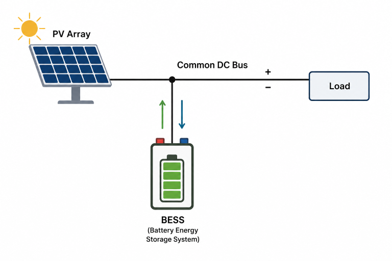
\includegraphics[width=0.65\textwidth]{Figures/Figure 1.16.png}
    \caption{Conceptual integration of a Battery Energy Storage System (BESS) with a common DC bus in a photovoltaic-based energy system.}
    \label{fig:bess_integration}
\end{figure}

\subsection{Operating Principle of Battery Energy Storage Systems}
The operating principle of a Battery Energy Storage System (BESS) is based on reversible electrochemical reactions that enable the storage and release of electrical energy. During the charging process, electrical energy supplied from an external source is converted into chemical energy and stored within the battery cells. During discharging, the stored chemical energy is converted back into electrical energy to supply the connected load.

\begin{figure}[H]
    \centering
    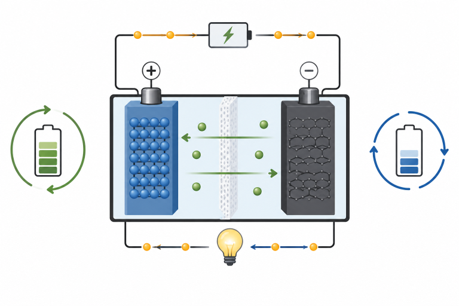
\includegraphics[width=0.65\textwidth]{Figures/Figure 1.17.png}
    \caption{Electrochemical operating principle of a battery energy storage system during charging and discharging processes.}
    \label{fig:bess_electrochemistry}
\end{figure}

The charging and discharging processes are continuously monitored and controlled by the Battery Management System (BMS), which regulates key operating parameters such as voltage, current, temperature, and State of Charge (SOC). Proper battery management improves operational safety, prevents overcharging and excessive discharging, and contributes to extending the battery lifetime while maintaining reliable system performance.

\subsection{Battery Technologies}
Various battery technologies have been developed for energy storage applications, each offering different characteristics in terms of energy density, efficiency, lifetime, cost, and maintenance requirements. The selection of a suitable battery technology depends on the intended application, operating conditions, and system requirements. Among the most widely used battery technologies are lead-acid, nickel-metal hydride (NiMH), and lithium-ion batteries\cite{dunn2011}.

Among the available battery technologies, lithium-ion batteries exhibit the highest energy density, round-trip efficiency, and cycle life. In addition, they offer low maintenance requirements and excellent electrochemical performance, making them the preferred choice for modern photovoltaic energy storage systems despite their relatively higher initial cost.

\begin{table}[H]
    \centering
    \caption{Comparison of Common Battery Technologies.}
    \label{tab:battery_technologies}
    
    \renewcommand{\arraystretch}{1.4} % Nice vertical padding between rows
    \rowcolors{2}{white}{gray!8} % Clean alternating zebra stripes
    
    % Proportional constraints: Gives more room to the first column 
    % and splits the remaining width perfectly across the numerical data columns
    \begin{tabularx}{\textwidth}{
        >{\hsize=1.4\hsize\raggedright\arraybackslash}X 
        >{\hsize=0.9\hsize\raggedright\arraybackslash}X 
        >{\hsize=0.9\hsize\raggedright\arraybackslash}X 
        >{\hsize=0.9\hsize\raggedright\arraybackslash}X
        >{\hsize=0.9\hsize\raggedright\arraybackslash}X
    }
        \toprule
        \textbf{Battery Technology} & \textbf{Energy Density} & \textbf{Efficiency} & \textbf{Cycle Life} & \textbf{Relative Cost} \\
         & \textbf{(Wh/kg)} & \textbf{(\%)} & \textbf{(cycles)} &  \\
        \midrule
        Lead-Acid & 30–50 & 70–85 & 500–1,000 & Low \\
        Nickel-Metal Hydride (NiMH) & 60–120 & 65–80 & 500–2,000 & Moderate \\
        Lithium-Ion & 150–250 & 90–95 & 2,000–7,000 & High \\
        \bottomrule
    \end{tabularx}
\end{table}

\subsection{Lithium-Ion Batteries}
Lithium-ion (Li-ion) batteries are the most widely used rechargeable batteries in modern energy storage applications due to their high energy density, high efficiency, long cycle life, and low self-discharge rate. Compared with conventional battery technologies, lithium-ion batteries provide superior electrochemical performance while requiring minimal maintenance. These characteristics have made them the preferred choice for photovoltaic energy storage systems, electric vehicles, and other applications requiring reliable and efficient energy storage\cite{dunn2011}.

The operation of a lithium-ion battery is based on the movement of lithium ions between the anode and the cathode through the electrolyte. During charging, lithium ions migrate from the cathode to the anode, where they are stored within the electrode material. During discharging, the ions move back to the cathode while electrons flow through the external circuit, delivering electrical energy to the connected load. This reversible electrochemical process enables repeated charging and discharging cycles with high efficiency and excellent energy storage capability.

\begin{figure}[H]
    \centering
    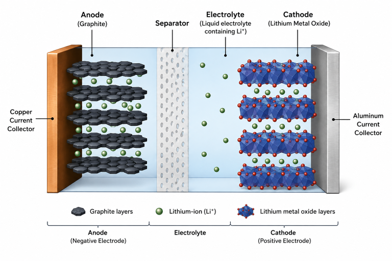
\includegraphics[width=0.7\textwidth]{Figures/Figure 1.18.png}
    \caption{Schematic structure of a lithium-ion battery showing its main components, including the anode, cathode, separator, electrolyte, and current collectors.}
    \label{fig:liion_structure}
\end{figure}
\section{Utility Grid}
The utility grid is an interconnected electrical network responsible for transmitting and distributing electrical power from generation stations to end users. It consists of generation units, high-voltage transmission lines, substations, and distribution networks operating together to ensure reliable, stable, and continuous electricity supply. Modern utility grids are designed to maintain system stability while accommodating continuously varying load demands.
\subsection{Overview of the Utility Grid}
The primary objective of the utility grid is to deliver electrical energy while maintaining stable voltage and frequency within specified operating limits. Electrical power generated at power plants is transmitted over long distances using high-voltage transmission networks to minimize transmission losses before being distributed to consumers through medium- and low-voltage distribution systems. Grid operation is continuously supervised using monitoring, protection, and control systems to ensure secure and reliable power delivery
\begin{figure}[H]
    \centering
    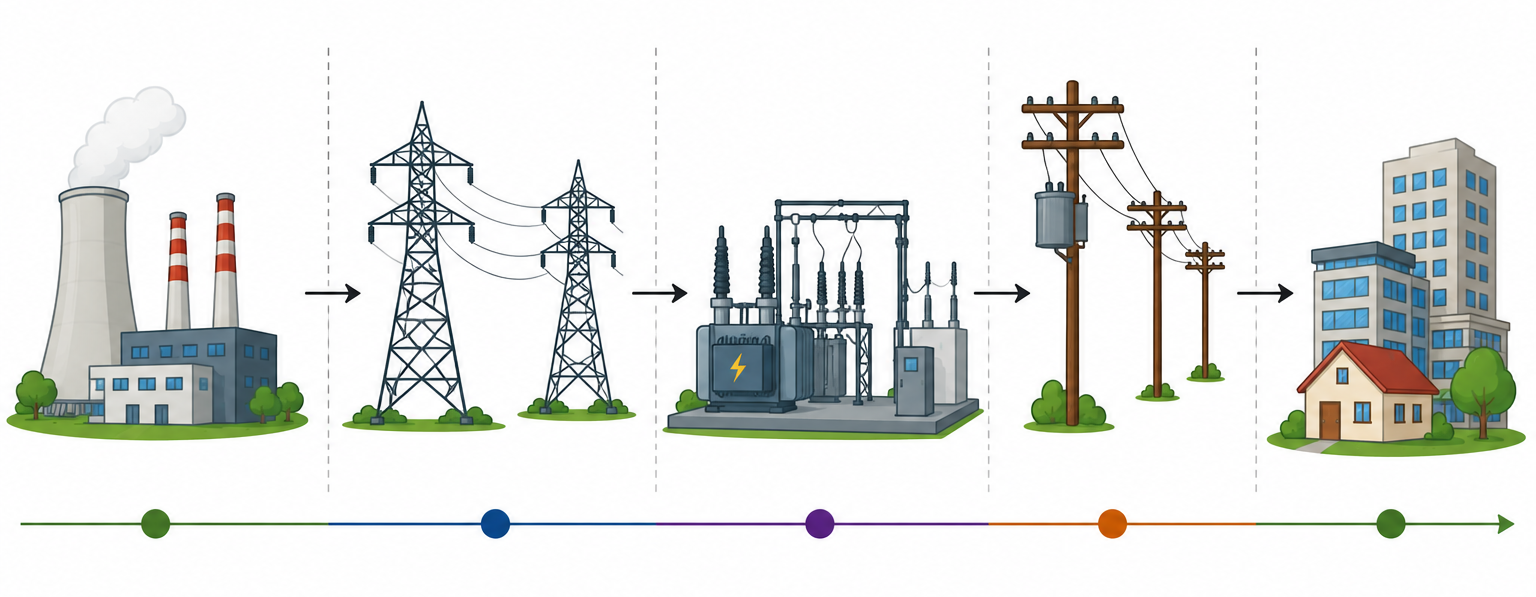
\includegraphics[width=\textwidth]{Figures/Grid .png}
    \caption{General structure of a utility grid illustrating the flow of electrical power from generation to end users through transmission, substations, and distribution networks.}
    \label{fig:utility_grid_structure}
\end{figure}
\subsection{Operating Principle of the Utility Grid}
The operation of the utility grid is based on maintaining a continuous balance between electrical power generation and load demand. Power generated from different generating stations is synchronized and transmitted through interconnected transmission networks before reaching distribution systems and end users. System operators continuously regulate power flow, voltage, and frequency to ensure stable operation under varying loading conditions while maintaining power quality and system reliability.

\newpage
\subsection{Characteristics of Modern Utility Grids}
Modern utility grids are characterized by high reliability, large power transmission capability, and extensive geographical coverage. The integration of advanced monitoring systems, communication technologies, and power electronic converters has significantly improved grid flexibility and operational efficiency. These developments have enabled modern utility grids to accommodate distributed generation, renewable energy sources, and bidirectional power flow while maintaining secure and stable system operation\cite{rehmani2018}.

\section{Electric Vehicle Charging Systems}
Electric vehicles (EVs) have emerged as a promising solution for reducing greenhouse gas emissions and decreasing dependence on fossil fuels. Their rapid global adoption has increased the demand for reliable and efficient charging infrastructure capable of supporting sustainable transportation systems.

\subsection{Overview of Electric Vehicles}
An electric vehicle (EV) is a vehicle powered wholly or partially by electrical energy stored in rechargeable batteries. Unlike conventional internal combustion engine vehicles, electric vehicles use electric motors for propulsion, resulting in higher energy efficiency, lower operating costs, and zero tailpipe emissions. These advantages have accelerated the adoption of electric vehicles in both residential and commercial transportation sectors.

The rapid advancement of battery technologies, continuous improvements in charging infrastructure, and growing environmental awareness have significantly accelerated the global adoption of electric vehicles. As a result, electric vehicles have become a key component of sustainable transportation systems, offering an effective solution for reducing greenhouse gas emissions and improving overall energy efficiency\cite{tie2013,emadi2015}.


\begin{figure}[H]
    \centering
    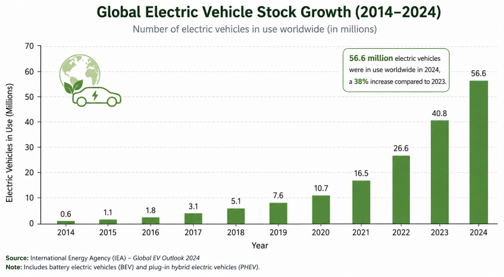
\includegraphics[width=0.75\textwidth]{Figures/Figure 1.19.png}
    \caption{Global growth of electric vehicle stock between 2014 and 2024 (adapted from \cite{iea2024}).}
    \label{fig:ev_growth}
\end{figure}

\newpage

\subsection{Electric Vehicle Charging}
Electric vehicle charging is the process of transferring electrical energy from an external power source to the battery pack of an electric vehicle. The charging process is performed through dedicated charging equipment that safely delivers electrical energy while monitoring charging parameters to ensure reliable and efficient battery operation.

Electric vehicle charging stations can be supplied from different energy sources, including the utility grid, renewable energy systems, or hybrid energy systems. Among these, photovoltaic-powered charging stations have gained considerable attention because they utilize clean solar energy to charge electric vehicles, thereby reducing greenhouse gas emissions and decreasing dependence on conventional electricity generation\cite{tie2013}.

\begin{figure}[H]
    \centering
    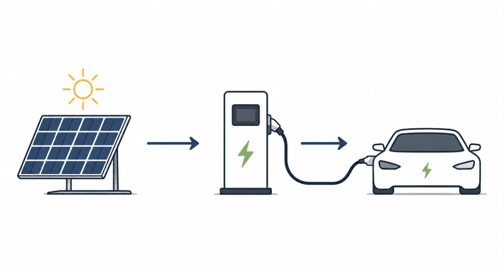
\includegraphics[width=0.65\textwidth]{Figures/Figure 1.20.png}
    \caption{Conceptual illustration of a photovoltaic-powered electric vehicle charging system.}
    \label{fig:pv_ev_charging}
\end{figure}

Depending on the charging power and charging duration, electric vehicle charging systems are generally classified into different charging levels. These charging levels provide various charging speeds to satisfy different user requirements and application scenarios.

\subsection{Electric Vehicle Charging Levels}
Electric vehicle charging systems are commonly classified according to the charging power, supply voltage, and charging duration. Different charging levels have been developed to satisfy various charging requirements ranging from residential overnight charging to rapid public charging stations. The selection of an appropriate charging level depends on factors such as battery capacity, charging time, installation cost, and application requirements.

\begin{table}[H]
    \centering
    \caption{Comparison of Electric Vehicle Charging Levels.}
    \label{tab:charging_levels}
    
    \renewcommand{\arraystretch}{1.4} % Nice vertical padding between rows
    \rowcolors{2}{white}{gray!8} % Clean alternating zebra stripes
    
    % Proportional constraints: Allocates balanced page-width ratios 
    % so that columns wrap text beautifully and fit within your margins
    \begin{tabularx}{\textwidth}{
        >{\hsize=1.1\hsize\raggedright\arraybackslash}X 
        >{\hsize=1.0\hsize\raggedright\arraybackslash}X 
        >{\hsize=0.8\hsize\raggedright\arraybackslash}X 
        >{\hsize=1.0\hsize\raggedright\arraybackslash}X
        >{\hsize=1.1\hsize\raggedright\arraybackslash}X
    }
        \toprule
        \textbf{Charging Level} & \textbf{Supply} & \textbf{Power} & \textbf{Charging Time} & \textbf{Typical Application} \\
        \midrule
        Level 1 & 120 V AC & 1.4–1.9 kW & 8–20 h & Residential \\
        Level 2 & 208–240 V AC & 3.3–22 kW & 2–8 h & Residential / Commercial \\
        DC Fast Charging & 400–1000 V DC & 25–350 kW & 20–60 min & Public Charging Stations \\
        \bottomrule
    \end{tabularx}
\end{table}

As summarized in Table 3, Level 1 charging is mainly intended for overnight residential charging due to its low charging power. Level 2 charging provides a practical balance between charging speed and installation cost, making it suitable for residential and commercial applications. In contrast, DC fast charging delivers significantly higher charging power, enabling rapid battery charging in public charging stations where minimizing charging time is a priority.

\section{Common DC Bus Architecture}
A common DC bus architecture is widely employed in photovoltaic-powered electric vehicle charging systems to integrate multiple energy sources and loads into a unified electrical platform. In this configuration, the photovoltaic (PV) array, battery energy storage system (BESS), utility grid, and electric vehicle (EV) charger are interconnected through a common DC link. The utility grid is interfaced with the DC bus via a bidirectional grid-tied AC/DC converter, enabling controlled power exchange between the charging station and the electrical network. This architecture minimizes unnecessary power conversion stages, improves energy management, and enhances overall system flexibility.
\begin{figure}[H]
    \centering
    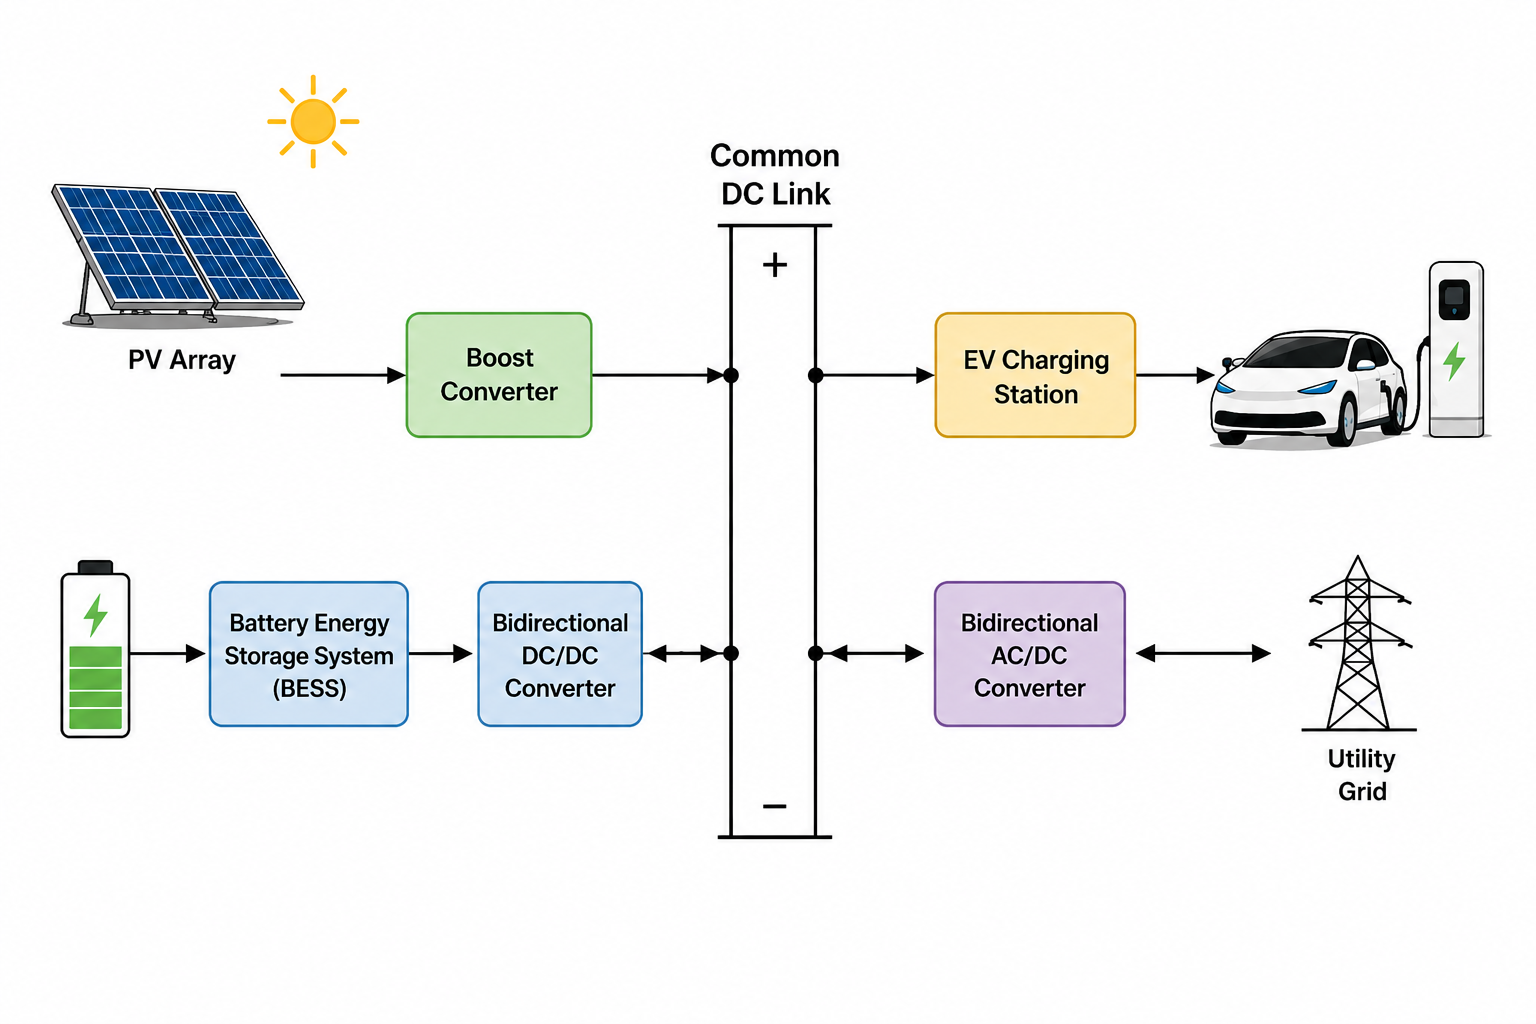
\includegraphics[width=0.9\textwidth]{Figures/system.png}
    \caption{General architecture of a photovoltaic-powered electric vehicle charging system based on a common DC bus.}
    \label{fig:dc_bus_architecture}
\end{figure}
The operating principle of the proposed system is based on coordinated power exchange through the common DC link. Electrical energy generated by the photovoltaic array is boosted to the required DC voltage and supplied to the DC bus. The EV charger draws power directly from the DC link to charge the vehicle battery. The Battery Energy Storage System (BESS) stores excess photovoltaic energy during periods of surplus generation and discharges it when additional power is required. Meanwhile, the utility grid exchanges power with the DC link through a bidirectional AC/DC converter. The grid supplies energy when the available photovoltaic generation and battery storage are insufficient to satisfy the charging demand, while excess energy can be exported back to the utility grid under appropriate operating conditions. This coordinated operation improves power management, increases overall system efficiency, and ensures reliable EV charging under varying operating conditions.
\section{Chapter Summary}
This chapter provided the theoretical background of the proposed photovoltaic-powered electric vehicle charging system. It reviewed the operating principles and essential characteristics of photovoltaic systems, battery energy storage systems, and electric vehicle charging systems. In addition, the common DC bus architecture was introduced to demonstrate the integration and power flow among the system components. This background serves as the foundation for the system design, modeling, control strategy, and simulation results presented in the subsequent chapters.

\chapter{Power Electronics Topologies and MPPT Theory}

% =========================================================================
% SECTION 2.1: DC-DC CONVERTERS
% =========================================================================
\section{DC-DC Converters}

\subsection{Introduction to DC-DC Converters}
DC-DC converters are fundamental power electronics topologies critical to modern electrical architecture and energy management systems. Their primary function is to transform a direct current (DC) input voltage from one level to a regulated, stabilized output level, ensuring reliable power delivery to downstream subsystems. In practical applications, the input voltage source is rarely static; factors such as battery state-of-charge (SoC) degradation over time, environmental variations in photovoltaic (PV) arrays, and dynamic load transient conditions necessitate high-performance regulation.

Traditional linear regulators achieve voltage regulation by dissipating excess power as heat across a resistive pass element, inherently limiting their efficiency and thermal performance. In contrast, switching DC-DC converters utilize high-frequency semiconductor switches, energy storage elements (inductors and capacitors), and periodic control strategies to achieve superior conversion efficiency, often exceeding 90\% to 95\%. This minimization of power loss is vital for thermal management, reducing cooling requirements, and maximizing overall system longevity.

Furthermore, switching topologies offer structural flexibility, enabling step-down (Buck), step-up (Boost), or bidirectional (Two-Quadrant Chopper) power flows. Where system safety or noise mitigation is paramount, these converters can incorporate galvanic isolation via high-frequency transformers to decouple input and output grounds, protecting sensitive digital control logic from high-energy spikes. Non-isolated topologies, conversely, maintain a common ground and are highly favored in weight- and cost-sensitive applications due to their higher power density and reduced component count.

In this project, the implementation focuses on high-efficiency, non-isolated topologies essential for localized power distribution, specifically:
\begin{itemize}
    \item Buck Converter
    \item Boost Converter
    \item Interleaved Boost Converter
    \item Two-Quadrant Chopper
\end{itemize}

\newpage

\subsection{Types of DC-DC Converters}

\subsubsection{Buck Converter}
The Buck converter, or step-down chopper, is a foundational switching topology designed to deliver an output voltage lower than the applied input voltage ($U_{out} < E$).

\paragraph{Circuit Diagram:}

\begin{figure}[H]
    \centering
    
\includegraphics[width=0.75\textwidth]{Figures/Figure 2.1.png}
    \caption{The Buck Converter Circuit Diagram.}
    \label{fig:buck_circuit}
\end{figure}

\paragraph{Introduction and Principle of Operation:}
The operating principle of the buck converter involves controlled energy transfer from the input to the output through switches, an inductor, and a capacitor. A high-side switch (usually a MOSFET) and a low-side switch (typically a diode) are employed to control the current flow through the inductor. By adjusting the duty cycle of the high-side switch, the average output voltage can be regulated proportionally to the input voltage.

When the high-side switch is turned on, it allows current to flow through the inductor, which stores energy in its magnetic field. This stored energy is then transferred to the output, charging the output capacitor and powering the load. When the high-side switch is turned off and the low-side switch is turned on, the inductor's magnetic field collapses, releasing the stored energy and maintaining current flow to the load.

Assuming Continuous Conduction Mode (CCM), where the inductor current $i_L(t)$ remains strictly positive throughout the entire switching period ($T$), the circuit operates in two distinct intervals:
\begin{itemize}
    \item \textbf{Interval 1: Switch ON ($0 < t \le DT$):} When switch S is closed, diode D is reverse-biased by the input source E. Current flows from the source through inductor L and the parallel RC load network. During this interval, the inductor absorbs energy, and its current rises linearly from $i_{min} $ to $i_{max}$. The instantaneous inductor voltage is defined by:
    \begin{equation}
        V_L = E - U_{out}
    \end{equation}

    \newpage
    
    \item \textbf{Interval 2: Switch OFF ($DT < t \le T$):} When switch S opens, the commutating inductor opposes the sudden drop in current by reversing its voltage polarity. This forward-biases the freewheeling diode D, creating a closed path that allows the stored magnetic energy to discharge into the output capacitor and load. The inductor current falls linearly from $i_{max}$ to $i_{min}$. The instantaneous inductor voltage during this phase is:
    \begin{equation}
        V_L = -U_{out}
    \end{equation}
\end{itemize}

\begin{figure}[H]
    \centering
    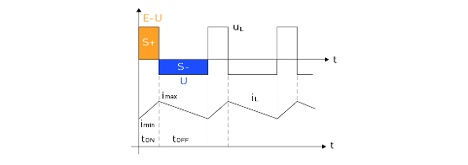
\includegraphics[width=0.75\textwidth]{Figures/Figure 2.2.png}
    \caption{The Buck Converter – Inductor Voltage and Current Versus Time Graph.}
    \label{fig:buck_waveforms1}
\end{figure}

\paragraph{Design Consideration and Calculations:}
The output voltage is determined by the duty cycle $D$:
\begin{equation}
    U = D \cdot E
\end{equation}

To limit the peak-to-peak inductor current ripple $\Delta I_L$, the minimum required inductance $L$ is governed by the switching frequency $f_s$ and the input voltage:
\begin{equation}
    L = \frac{(E - U) \cdot D}{\Delta I_L \cdot f_s}
\end{equation}

Similarly, the output filtering capacitance $C$ must mitigate the output voltage ripple $\Delta U$. The capacitance value is computed based on the allowable peak-to-peak ripple:
\begin{equation}
    C = \frac{\Delta I_L}{8 \cdot f_s \cdot \Delta U}
\end{equation}
The output capacitor plays a vital role in filtering the output voltage ripple and maintaining stability in the converter, depending directly on the intended output voltage ripple, the ripple current, and the switching frequency.

\newpage

% -------------------------------------------------------------------------
\subsubsection{Boost Converter}
The boost converter is a step-up switching topology utilized when the application demands an output voltage greater than the source input ($U > E$).

\paragraph{Circuit Diagram:}
\begin{figure}[H]
    \centering
    
\includegraphics[width=0.75\textwidth]{Figures/Figure 2.3.png}
    \caption{The Boost Converter Circuit Diagram – Interval $t_{ON}$.}
    \label{fig:buck_waveforms}
\end{figure}

\begin{figure}[H]
    \centering
    
\includegraphics[width=0.75\textwidth]{Figures/Figure 2.4.png}
    \caption{The Boost Converter Circuit Diagram – Interval $t_{OFF}$.}
    \label{fig:buck_waveformss}
\end{figure}

\paragraph{Introduction and Principle of Operation:}
Boost converters efficiently step up an input voltage to a higher output voltage by storing energy in an inductor during the switch-on phase and releasing it to the load during the switch-off phase. Power electronics applications requiring a greater output voltage than the input source depend heavily on this topology. The operational stages are broken down as follows:

\begin{itemize}
    \item \textbf{Switch-on period ($S$ closed, diode reverse biased):} Switch S is closed, shorting the right side of the inductor directly to the return path. Diode D is reverse-biased by the output voltage U, isolating the load stage. The input voltage E is applied entirely across L, causing the inductor current to ramp upward linearly from $i_{min}$ to $i_{max}$, storing energy within its magnetic core.
    \begin{equation}
        u_L = E
    \end{equation}
    \begin{equation}
        \Delta I_L = \frac{E \cdot t_{ON}}{L}
    \end{equation}

    \newpage
    
    \item \textbf{Switch-off period ($S$ open, diode forward biased):} Switch S opens. To sustain current continuity, the inductor induces a positive voltage that adds in-series with the source voltage E. Diode D becomes forward-biased, dumping the combined energy of the source and the inductor into the output capacitor and load.
    \begin{equation}
        u_L = E - U
    \end{equation}
\end{itemize}

By equating the inductor current changes for both stages, the voltage conversion relationship for the boost converter yields:
\begin{equation}
    U = \frac{E}{1 - D}
\end{equation}
where $D$ is the duty cycle, defined as the ratio of the switch-on time ($t_{on}$) to the total switching period ($T$).

\begin{figure}[H]
    \centering
    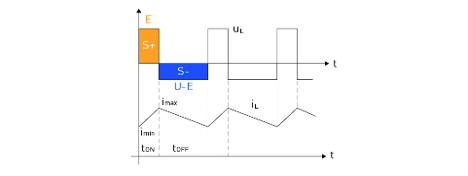
\includegraphics[width=0.75\textwidth]{Figures/Figure 2.5.png}
    \caption{The Boost Converter - Inductor Voltage and Current Versus Time Graph.}
    \label{fig:boost_waveforms}
\end{figure}

\paragraph{Design Consideration and Calculations:}
In continuous conduction mode (CCM), the duty cycle $D$ determines the voltage step-up relationship as follows:
\begin{equation}
    D = \frac{U - E}{U}
\end{equation}
This equation is valid for the continuous conduction mode (CCM) operation. The duty cycle is important for selecting the appropriate switching frequency and inductor value.
\\
\\
The average inductor current matches the average input current ($I_L = I_{in}$). The inductor value $L$ required to restrict current ripples to a target percentage is calculated using:
\begin{equation}
    L = \frac{E \cdot D}{\Delta I_L \cdot f_s}
\end{equation}

The output capacitor provides sole power to the load during the switch-on period $t_{ON}$. Therefore, to restrict the output voltage ripple $\Delta U$, the capacitance is sized as follows:
\begin{equation}
    C = \frac{I_{out} \cdot D}{\Delta U \cdot f_s}
\end{equation}



% -------------------------------------------------------------------------
\subsubsection{Interleaved Boost Converter}
When applications scale to high power levels, standard single-phase boost converters face severe limitations, including high thermal stresses on semiconductor components, large passive component footprints, and significant input current ripples. To overcome these constraints, an Interleaved Boost Converter (IBC) topology is deployed [11].

\paragraph{Circuit Diagram:}
\begin{figure}[H]
    \centering
    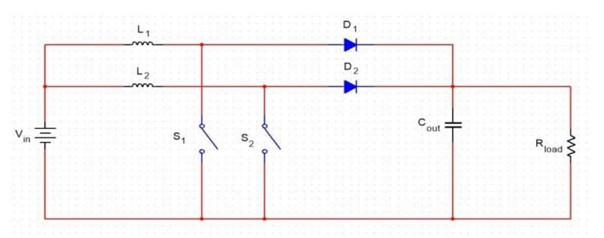
\includegraphics[width=0.75\textwidth]{Figures/Figure 2.6.jpg}
    \caption{Interleaved DC-DC Boost Converter Circuit Diagram.}
    \label{fig:ibc_circuit}
\end{figure}

\paragraph{Introduction and Principle of Operation:}
The multiphase interleaved configuration splits the power path into parallel branches ($N$ phases). For a standard two-phase interleaved system, two identical boost branches operate at the same switching frequency $f_s$, but their gate drive signals are intentionally phase-shifted by $180^\circ$ ($\frac{360^\circ}{N}$) [11].

Because the inductor ripple currents $i_1$ and $i_2$ are out of phase, their ripples structurally cancel each other out when summing at the input node, effectively doubling the apparent ripple frequency to $2f_s$ [11].

The two-phase IBC steps through four discrete operating modes based on the overlapping states of switches $S_1$ and $S_2$:
\begin{itemize}
    \item \textbf{Mode 1 ($S_1$ ON, $S_2$ ON):} Both switches are closed and diodes $D_1$ and $D_2$ are reverse-biased. Both inductors $L_1$ and $L_2$ absorb energy simultaneously from the input source $V_{in}$, with both currents rising linearly. The output load is supported entirely by the filtering capacitor $C_{out}$.
    \begin{figure}[H]
    \centering
    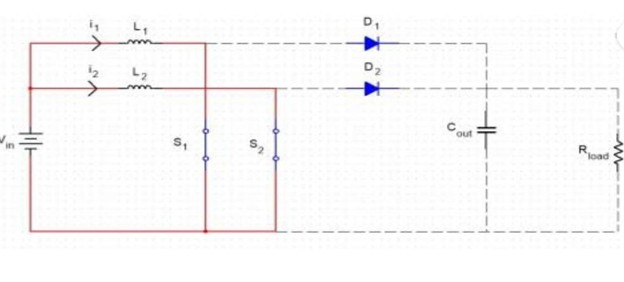
\includegraphics[width=0.65\textwidth]{Figures/Figure 2.7.jpg}
    \caption{Mode 1.}
    \label{fig:ibc_circuit2}
\end{figure}
    \item \textbf{Mode 2 ($S_1$ ON, $S_2$ OFF):} Switch $S_1$ remains closed, continuing to charge $L_1$, while switch $S_2$ opens, forcing diode $D_2$ into conduction. Inductor $L_2$ enters its discharge phase, transferring its stored energy along with the source to the output stage.
    \begin{figure}[H]
    \centering
    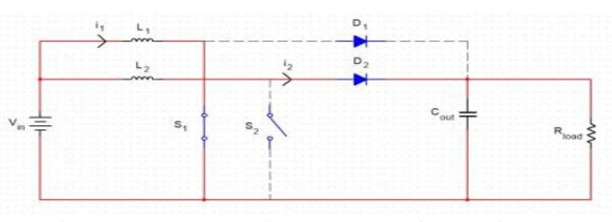
\includegraphics[width=0.75\textwidth]{Figures/Figure 2.8.jpg}
    \caption{Mode 2.}
    \label{fig:ibc_circuit22}
\end{figure}
    \item \textbf{Mode 3 ($S_1$ OFF, $S_2$ ON):} Switch $S_1$ opens, forward-biasing $D_1$, which allows $L_1$ to discharge its accumulated energy into the load. Simultaneously, $S_2$ is closed, placing $L_2$ back into its charging cycle.
    \begin{figure}[H]
    \centering
    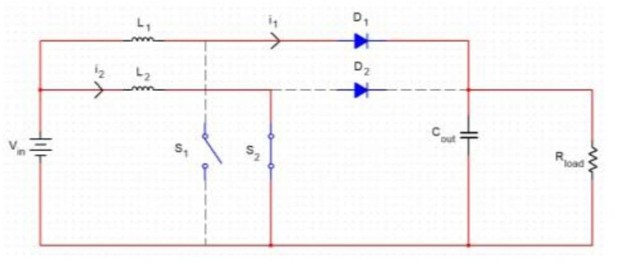
\includegraphics[width=0.75\textwidth]{Figures/Figure 2.9.jpg}
    \caption{Mode 3.}
    \label{fig:ibc_circuit3}
\end{figure}
    \item \textbf{Mode 4 ($S_1$ OFF, $S_2$ OFF):} Both switches are open (occurring when the operating duty cycle $D < 0.5$). Diodes $D_1$ and $D_2$ are forward-biased, causing both inductors to simultaneously discharge their energy into the output network.
\end{itemize}
\begin{figure}[H]
    \centering
    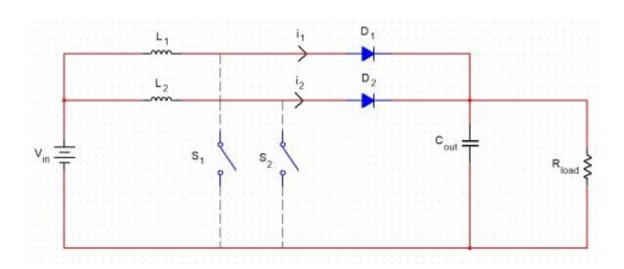
\includegraphics[width=0.75\textwidth]{Figures/Figure 2.10.jpg}
    \caption{Mode 4.}
    \label{fig:ibc_circuit4}
\end{figure}

\paragraph{Design Consideration and Calculations:}
The conversion duty cycle equation mirrors the conventional boost setup:
\begin{equation}
    D = \frac{V_{out} - V_{in}}{V_{out}}
\end{equation}
The total average input current is split equally among the $N=2$ phases:
\begin{equation}
    I_L = \frac{I_{in}}{2}
\end{equation}
Each phase inductor is sized independently using the single-phase ripple requirements:
\begin{equation}
    L_1 = L_2 = \frac{V_{in} \cdot D}{\Delta I_{L\_phase} \cdot f_s}
\end{equation}
The output filtering capacitance value is computed via:
\begin{equation}
    C_{out} = \frac{I_{out} \cdot D}{\Delta V_{out} \cdot f_s}
\end{equation}

So, Whenever high power, and high voltage gains are desired, single stage conventional boost converters are not sufficient as they produce high voltage and current ripples, increased switching stress and low conversion efficiency.
Interleaving technology in this regard can prove effective to meet these requirements with the benefits of the following [11];
\\
\\
-High voltage gain.
\\
-Input current ripple elimination and low conduction losses.
\\
-Reduced ripple output voltage.
\\
-Low voltage stress on switches.

% -------------------------------------------------------------------------
\subsubsection{Two-Quadrant Chopper}
The basic architecture consists of two fully controlled semiconductor switches $S_1, S_2$ connected in series across the primary DC link, with anti-parallel freewheeling diodes ($D_1, D_2$) paired across each switch. The load network is characterized by an inductive-resistive filter acting in series with a secondary voltage source $E_{load}$.

\paragraph{Circuit Diagram:}
\begin{figure}[H]
    \centering
    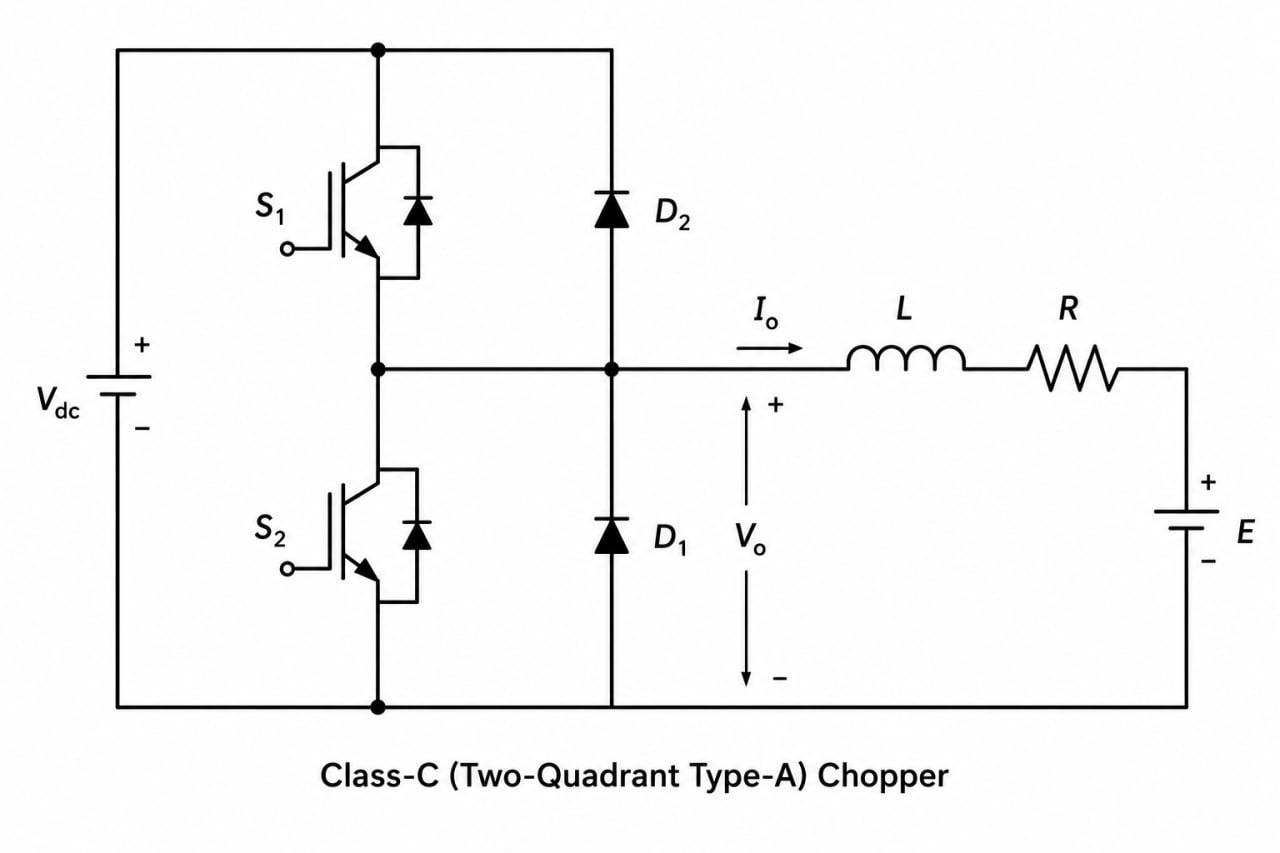
\includegraphics[width=0.5\textwidth]{Figures/Figure 2.11.jpg}
    \caption{Two Quadrant Chopper Circuit Diagram.}
    \label{fig:two_quad_circuit}
\end{figure}

\paragraph{Introduction and Principle of Operation:}
A Class-C chopper is a two-quadrant chopper operating in the first and second quadrants of the output voltage and current plane. Structurally, it represents a parallel combination of Class-A (step-down) and Class-B (step-up) choppers arranged in a complementary half-bridge configuration. This configuration allows for reversible power flow while maintaining a unipolar positive output voltage polarity. To prevent destructive shoot-through faults across the DC link, the gate drive signals for $S_1$ and $S_2$ must be mutually exclusive with an integrated dead-time interval.

\begin{itemize}
    \item \textbf{First Quadrant Operation (Forward Power Flow / Buck Mode):} Both $V_O$ and $I_o$ must remain positive, channeling power from the source $V_{dc}$ to the load.
    \begin{itemize}
        \item \textit{Interval 1 ($S_1$ ON, $S_2$ OFF):} When switch $S_1$ is active, the load is tied directly to the input source ($V_O = V_{dc}$), causing the inductor to store magnetic energy forwardly.
        \item \textit{Interval 2 ($S_1$ OFF, $S_2$ OFF):} When $S_1$ turns off, the inductor forward-biases freewheeling diode $D_1$. The current decays linearly through $D_1$ in the forward direction, forcing terminal voltage down to zero ($V_O = 0$).
    \end{itemize}
    
    \begin{figure}[H]
    \centering
    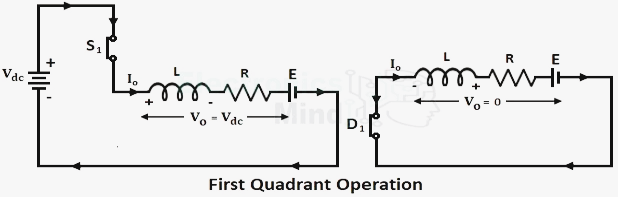
\includegraphics[width=0.55\textwidth]{Figures/Figure 2.12.png}
    \caption{Two Quadrant Chopper First Quadrant Operation.}
    \label{fig:two_quad_circuit2}
\end{figure}
    
    \item \textbf{Second Quadrant Operation (Reverse Power Flow / Boost Mode):} Terminal voltage $V_O$ remains positive, but the load current reverses direction ($-I_o$), requiring the active load source $E_{load}$ to drive energy back into the primary supply.
    \begin{itemize}
        \item \textit{Interval 1 ($S_2$ ON, $S_1$ OFF):} Switch $S_2$ turns on, short-circuiting the loop containing the inductor, load resistance, and active source $E_{load}$ ($V_O = 0$), storing energy inside the inductor negatively.
        \item \textit{Interval 2 ($S_2$ OFF, $S_1$ OFF):} When $S_2$ opens, the inductor's magnetic field collapses and forces diode $D_2$ into conduction, discharging energy back into the main supply link ($V_O = V_{dc}$).
    \end{itemize}
\end{itemize}

\begin{figure}[H]
    \centering
    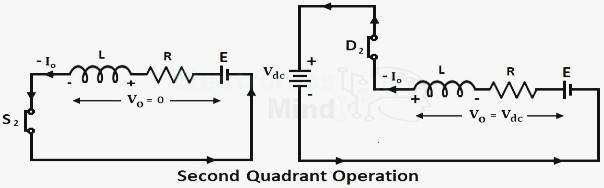
\includegraphics[width=0.55\textwidth]{Figures/Figure 2.13.jpg}
    \caption{Two Quadrant Chopper Second Quadrant Operation.}
    \label{fig:two_quad_circuit3}
\end{figure}

The continuous conduction mode transitions through four specific semiconductor states: $V_O=V_{dc}$ and $I_o>0$ (S1 conducting); $V_O=0$ and $I_o>0$ (D1 conducting); $V_O=0$ and $I_o<0$ (S2 conducting); and $V_O=V_{dc}$ and $I_o<0$ (D2 conducting).

\begin{figure}[H]
    \centering
    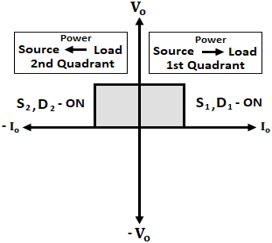
\includegraphics[width=0.55\textwidth]{Figures/Figure 2.14.png}
    \caption{Two Quadrant Operation.}
    \label{fig:two_quad_circuit4}
\end{figure}

Therefore, the output voltage $V_O = +V_{dc}$ (i.e., $V_O$ is positive) when $S_1$ or $D_2$ conducts, and $V_O$ is zero when $D_1$ or $S_2$ conducts. The output current $I_o$ is positive when $S_1$ or $D_1$ conducts, and $I_o$ is negative when $S_2$ or $D_2$ conducts. 
The waveforms of the Class-C chopper are illustrated below:

\begin{figure}[H]
    \centering
    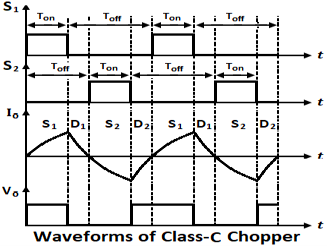
\includegraphics[width=0.6\textwidth]{Figures/Figure 2.15.png}
    \caption{Two-Quadrant Chopper Waveforms.}
    \label{fig:two_quad_waveforms}
\end{figure}

\newpage

In the above waveforms, when $S_1$ is ON, $I_o$ increases gradually to its maximum value and $V_O$ is positive. When $S_1$ is OFF, $V_O$ becomes zero and $I_o$ decreases gradually through $D_1$, which represents the discharge current of the inductor in the forward direction. When $S_2$ is ON, $V_O$ remains zero and $I_o$ increases negatively due to current flow in the reverse direction. When $S_2$ is OFF, $V_O$ becomes positive and $I_o$ decreases gradually from its negative maximum through $D_2$, which represents the discharge current of the inductor in the reverse direction.

The continuous conduction mode transitions through four specific semiconductor conduction states over a complete switching cycle:
\begin{itemize}
    \item $V_O = V_{dc}$ and $I_o > 0$ when $S_1$ is conducting.
    \item $V_O = 0$ and $I_o > 0$ when $D_1$ is conducting.
    \item $V_O = 0$ and $I_o < 0$ when $S_2$ is conducting.
    \item $V_O = V_{dc}$ and $I_o < 0$ when $D_2$ is conducting.
\end{itemize}

Since the output voltage is always positive and the output current can be either positive or negative, this topology represents a reversible power flow. Power flows from the source to the load when the chopper operates in the first quadrant, whereas power flows from the load back to the source when the chopper operates in the second quadrant. Additionally, extreme care must be taken to ensure that both switches are never turned ON at the same time, as this results in a catastrophic cross-conduction (shoot-through) short-circuit across the DC supply source.

\paragraph{Design Consideration and Calculations:}
The smoothing inductor $L$ is sized to suppress the peak-to-peak current ripple $\Delta i_L$ under the worst-case operating scenarios across both modes:
\begin{align}
    L_{buck} &= \frac{E_{load} \cdot (1 - D_{buck})}{\Delta i_L \cdot f_{sw}} \\
    L_{boost} &= \frac{V_O \cdot (V_{dc} - V_O)}{\Delta I_o \cdot f_s \cdot V_{dc}}
\end{align}
To ensure steady-state stability across both modes, the final chosen inductor value must satisfy the maximum boundary envelope:
\begin{equation}
    L_{optimal} = \max(L_{buck}, L_{boost})
\end{equation}
\newpage
\subsection{Conclusion of Converter Topologies}
\begin{itemize}
    \item \textbf{Buck Converter:} Operates strictly as a step-down regulator, ideal for down-converting voltage for low-power digital control stages, but restricted to unidirectional current delivery.
    \item \textbf{Boost Converter:} Functions exclusively as a step-up topology for low-voltage inputs, though it experiences high ripples at elevated power levels.
    \item \textbf{Interleaved Boost Converter:} Enhances the conventional setup by paralleling multi-phase branches with an explicit spatial delay ($\frac{360^\circ}{N}$), canceling out ripple currents and reducing component sizing constraints.
    \item \textbf{Two-Quadrant Chopper:} Couples step-down and step-up traits into a cohesive half-bridge structure, managing current reversibility while maintaining unipolar positive voltage to achieve seamless bidirectional transitions essential for battery energy storage systems (BESS) and electric vehicle (EV) charging stations.
\end{itemize}
% =========================================================================
% SECTION 2.2: MPPT THEORY
% =========================================================================
\section{MPPT Theory}

\subsection{Introduction to MPPT}
Photovoltaic (PV) arrays are fundamentally non-linear power sources. Unlike a standard DC power supply or a battery, which can maintain a relatively stable voltage regardless of the load, the current and voltage output of a solar panel depends entirely on atmospheric conditions (solar irradiance and ambient temperature) and the electrical characteristic of the connected load.

If a PV module is connected directly to a fixed load (like a battery or a basic inverter input), the system will rarely operate at its maximum efficiency. The operating point will simply be the intersection of the load line and the PV module's Current-Voltage ($I$-$V$) curve. Because weather conditions change continuously throughout the day, this intersection point shifts, often forcing the solar panel to operate well below its true power capacity.

Maximum Power Point Tracking (MPPT) is an electronic control strategy, typically implemented within a DC-DC converter, designed to solve this exact problem. The primary purposes of an MPPT system are:

\begin{itemize}
    \item \textbf{Maximum Efficiency:} It continuously forces the PV array to operate at its Maximum Power Point (MPP), which is the unique point on the Power-Voltage ($P$-$V$) curve where the product of voltage ($V_{mpp}$) and current ($I_{mpp}$) yields the highest possible power output ($P_{max}$).
    \item \textbf{Impedance Matching:} By dynamically adjusting the duty cycle ($D$) of the switching power converter, the MPPT controller changes the \textit{apparent impedance} of the load as seen by the solar panel, matching it to the optimal internal impedance of the PV module.
    \item \textbf{Environmental Adaptation:} It ensures that even when clouds pass by or the temperature spikes (which drastically drops the panel's voltage output), the system instantly tracks the new peak power position without manual intervention.
\end{itemize}

\begin{figure}[H]
    \centering
    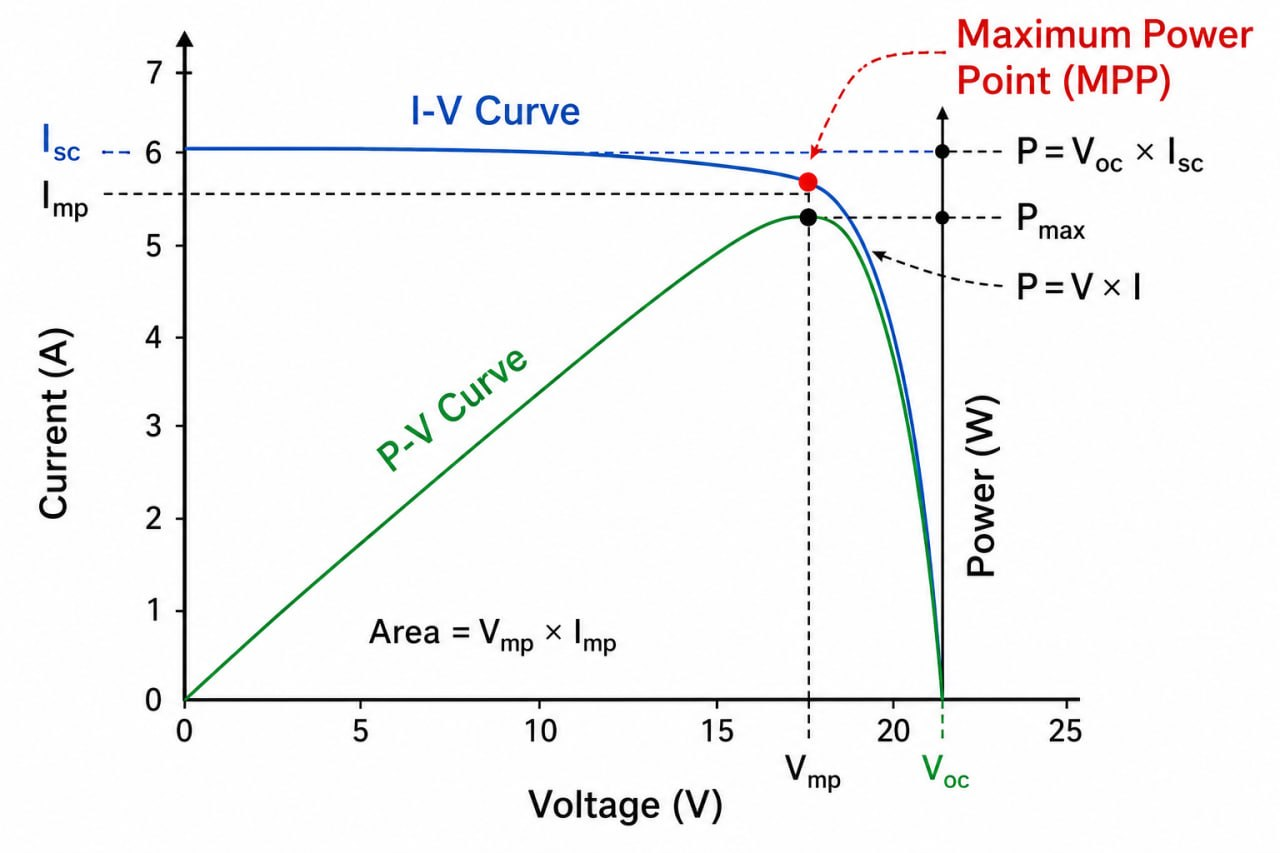
\includegraphics[width=0.7\textwidth]{Figures/Figure 2.16.jpg}
    \caption{P-V and I-V Characteristic Curves of a Photovoltaic Module.}
    \label{fig:pv_iv_curves}
\end{figure}

\subsection{Numerical Example of Power Tracking}
To understand how an MPPT algorithm tracks the peak power dynamically, we can analyze the behavior of a solar panel as its operating point shifts along the Power-Voltage ($P$-$V$) curve. Let us assume a starting condition and observe how changes in voltage ($V$) and current ($I$) affect the total output power ($P = V \times I$):

\begin{itemize}
    \item \textbf{Point 1 (Initial State):} The system operates at a voltage $V_1 = 20\text{ V}$ and a current $I_1 = 10\text{ A}$.
    \begin{equation}
        P_1 = 20\text{ V} \times 10\text{ A} = 200\text{ W}
    \end{equation}
    \item \textbf{Point 2 (Moving Up the Curve):} The algorithm changes the duty cycle, causing the voltage to slightly decrease to $V_2 = 19\text{ V}$, which allows the current to rise to $I_2 = 11\text{ A}$.
    \begin{equation}
        P_2 = 19\text{ V} \times 11\text{ A} = 209\text{ W}
    \end{equation}
    \textit{Observation:} Because $P_2 > P_1$ ($209\text{ W} > 200\text{ W}$), the power has \textit{increased}. This informs the controller that it is moving in the right direction toward the peak.
    \item \textbf{Point 3 (Past the Peak / Decreasing):} The algorithm attempts to change the operating point further in the same direction. The voltage drops to $V_3 = 17\text{ V}$, and the current rises to $I_3 = 12\text{ A}$.
    \begin{equation}
        P_3 = 17\text{ V} \times 12\text{ A} = 204\text{ W}
    \end{equation}
    \textit{Observation:} Because $P_3 < P_2$ ($204\text{ W} < 209\text{ W}$), the power has now \textit{decreased}. The controller realizes it has overshot the peak and must turn back toward Point 2.
\end{itemize}

\subsection{The Core Mathematical Condition}
This trial-and-error process is mathematically defined by analyzing the slope of the $P$-$V$ curve, which is the derivative of power with respect to voltage ($\frac{dP}{dV}$). As seen in the numerical example, the slope tells the controller exactly where it is relative to the Maximum Power Point (MPP):

\begin{itemize}
    \item \textbf{To the Left of the MPP ($\frac{dP}{dV} > 0$):} As voltage increases, power increases (this happened between Point 1 and Point 2). The controller needs to increase the voltage to reach the peak.
    \item \textbf{To the Right of the MPP ($\frac{dP}{dV} < 0$):} As voltage increases, power decreases (this happened when moving to Point 3). The controller needs to decrease the voltage to go back to the peak.
    \item \textbf{At the Maximum Power Point ($\frac{dP}{dV} = 0$):} The slope becomes perfectly flat. This is the ideal operating point ($P_{max} = 209\text{ W}$ in our example), where the system achieves maximum efficiency.
\end{itemize}

\begin{equation}
    \frac{dP}{dV} = 0
\end{equation}

\begin{figure}[H]
    \centering
    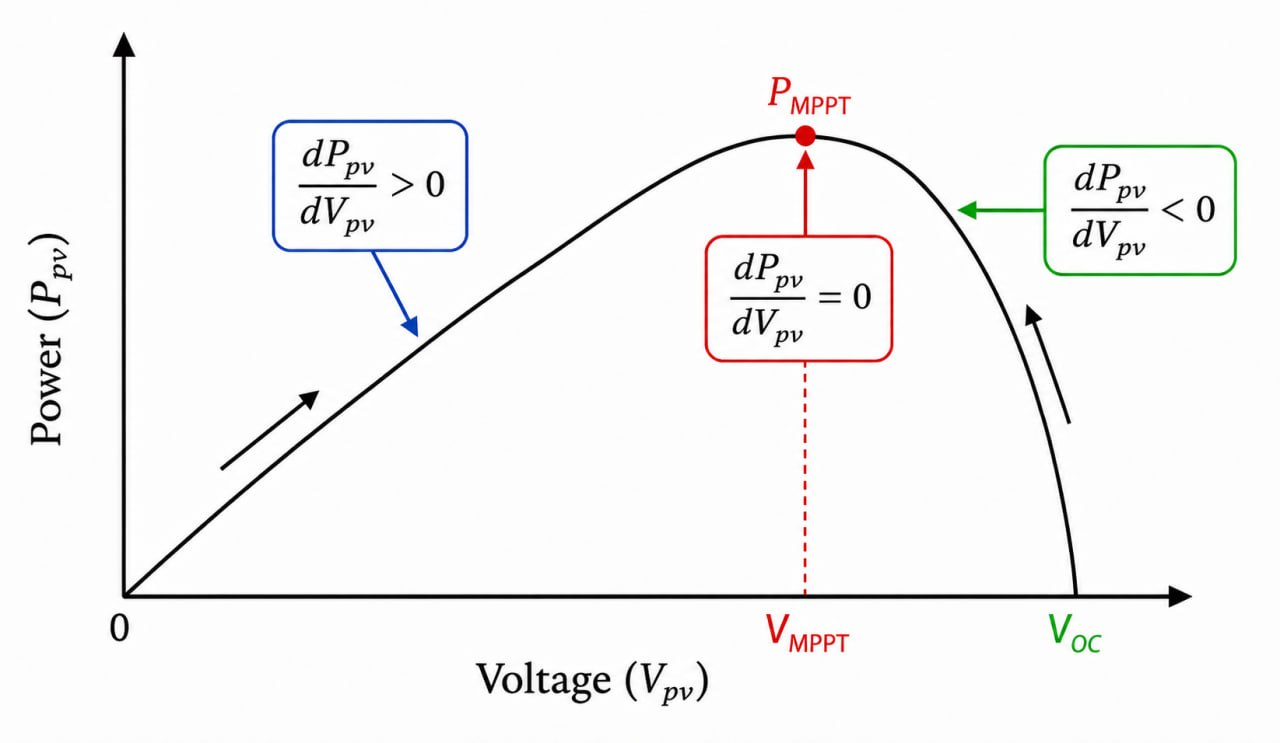
\includegraphics[width=0.65\textwidth]{Figures/Figure 2.17.jpg}
    \caption{MPPT Algorithm Operation Modes on the P-V Curve.}
    \label{fig:mppt_operation}
\end{figure}

\subsection{Classification of MPPT Algorithms}
To successfully satisfy the condition $\frac{dP}{dV} = 0$, various control strategies have been developed. These algorithms differ in complexity, tracking speed, sensor requirements, and their ability to handle uniform versus non-uniform solar irradiance.

\subsubsection{Perturb and Observe (P\&O)}
The Perturb and Observe (P\&O) algorithm, also known as the ``hill-climbing'' method, is the most widely used conventional MPPT technique due to its simplicity and low computational cost.

\paragraph{Operating Principle:}
The controller introduces a small perturbation (a deliberate step change) in the operating voltage of the PV array by modifying the converter's duty cycle, then measures the resulting power output. If the power increases ($\Delta P > 0$), the controller knows the perturbation moved the operating point closer to the peak and will continue to perturb the voltage in the \textit{same direction}. If the power decreases ($\Delta P < 0$), it means the operating point has overshot the peak, and the controller must \textit{reverse the direction} of the next perturbation.

\paragraph{Drawbacks:}
\begin{enumerate}
    \item \textbf{Steady-State Oscillation:} Once the algorithm reaches the true MPP, it cannot sit perfectly still. It continually perturbs the voltage back and forth across the peak, causing a small but constant power loss.
    \item \textbf{Tracking Failure under Rapid Weather Fluctuations:} If solar irradiance changes abruptly, the algorithm can get confused, tracking in the wrong direction and moving far away from the actual MPP.
\end{enumerate}

\begin{figure}[H]
    \centering
    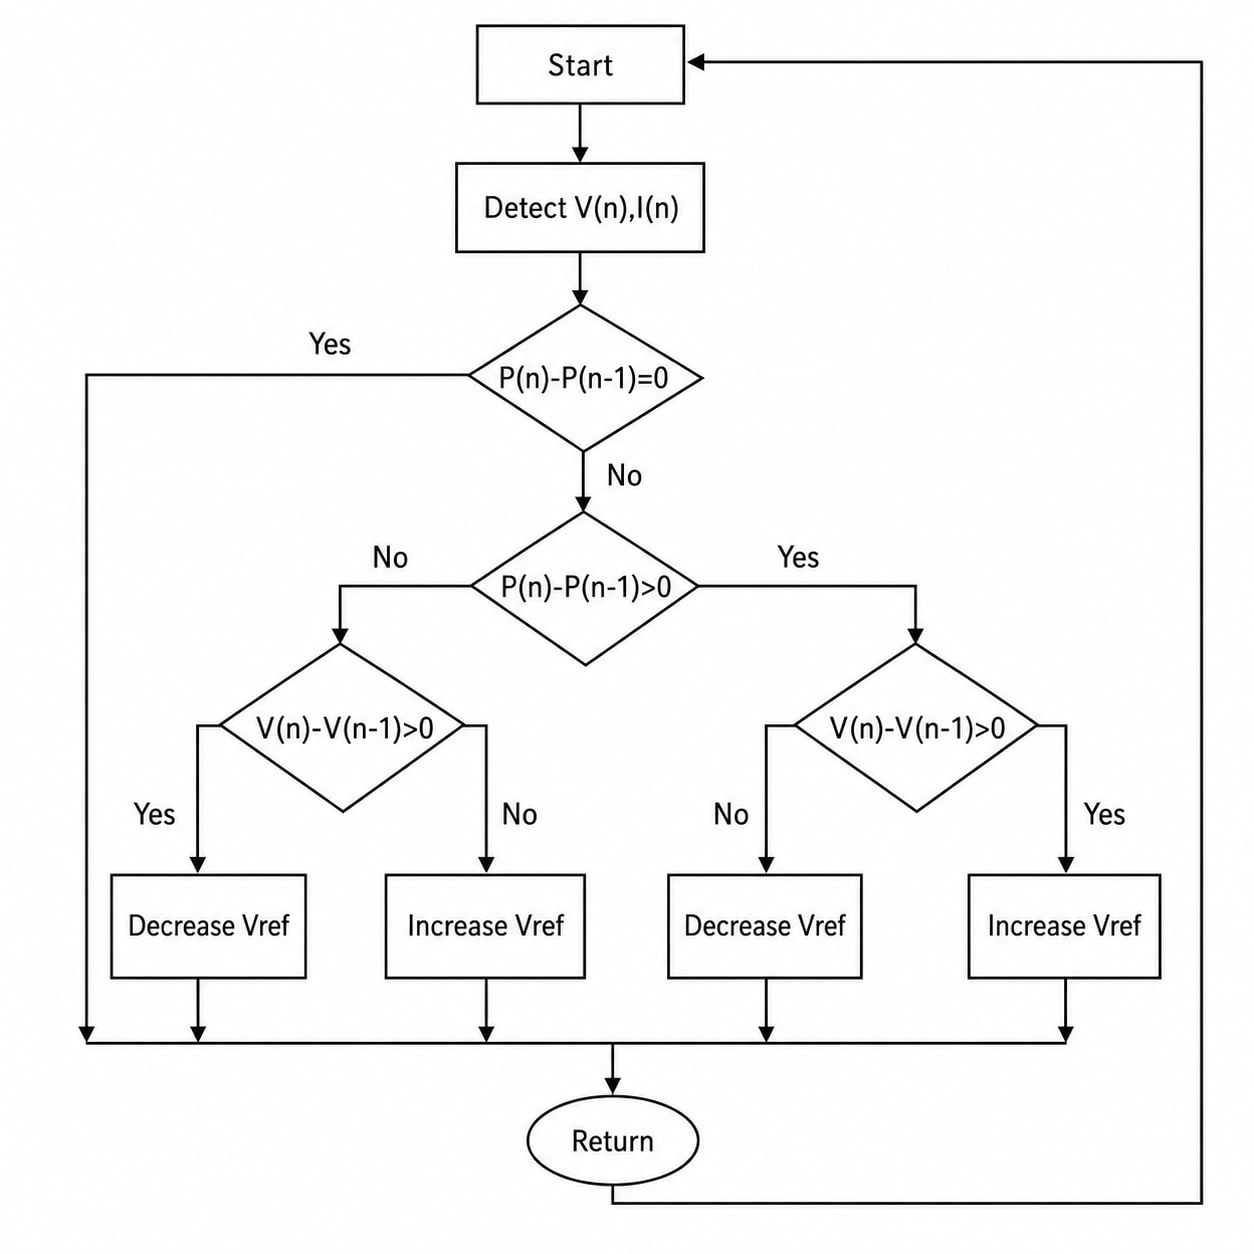
\includegraphics[width=0.6\textwidth]{Figures/Figure 2.18.jpg}
    \caption{Perturb and Observe (P\&O) Algorithm Flowchart.}
    \label{fig:po_flowchart}
\end{figure}

\subsubsection{Incremental Conductance (IncCond)}
The Incremental Conductance algorithm was designed to overcome the steady-state oscillation problem of P\&O. It uses the relationship between the instantaneous conductance ($\frac{I}{V}$) and the incremental conductance ($\frac{dI}{dV}$). As derived from the derivative of power ($P = VI$):

\begin{equation}
    \frac{dP}{dV} = I + V\frac{dI}{dV}
\end{equation}

By setting $\frac{dP}{dV} = 0$ at the maximum power point, the governing conditions are established as:
\begin{align}
    \frac{dI}{dV} &= -\frac{I}{V} \quad \text{(At the MPP)} \\
    \frac{dI}{dV} &> -\frac{I}{V} \quad \text{(Left of the MPP)} \\
    \frac{dI}{dV} &< -\frac{I}{V} \quad \text{(Right of the MPP)}
\end{align}

\paragraph{Operating Principle:}
The controller tracks the peak by comparing these two values. The major advantage of Incremental Conductance is that \textit{at the MPP, the perturbation stops completely}. The system maintains that exact operating point until a change in current ($\Delta I \neq 0$) is detected due to changing weather conditions.

\subsubsection{Global Scanning / Particle Swarm Optimization (PSO)}
Conventional methods like P\&O and IncCond assume the $P$-$V$ curve has only one single peak. However, if the EV charging station encounters \textit{Partial Shading} (e.g., a tree, building, or cloud casts a shadow over only part of the array), the $P$-$V$ curve warps. It creates multiple local peaks (Local MPPs) but only one true global peak (Global MPP).

\paragraph{The Problem with P\&O/IncCond:}
If a standard P\&O controller lands on a small local peak, it sees that $\frac{dP}{dV} = 0$. It gets stuck there indefinitely, completely missing the much larger global peak further down the curve.

\paragraph{The Global Scanning Solution:}
Soft-computing techniques like Particle Swarm Optimization (PSO) or global voltage sweeping algorithms send out ``scouts'' (virtual particles or rapid duty-cycle sweeps) across the entire voltage range from $0\text{ V}$ to $V_{oc}$. It scans the entire curve, identifies the absolute highest peak, and forces the converter to operate directly at the Global MPP.

\begin{figure}[H]
    \centering
    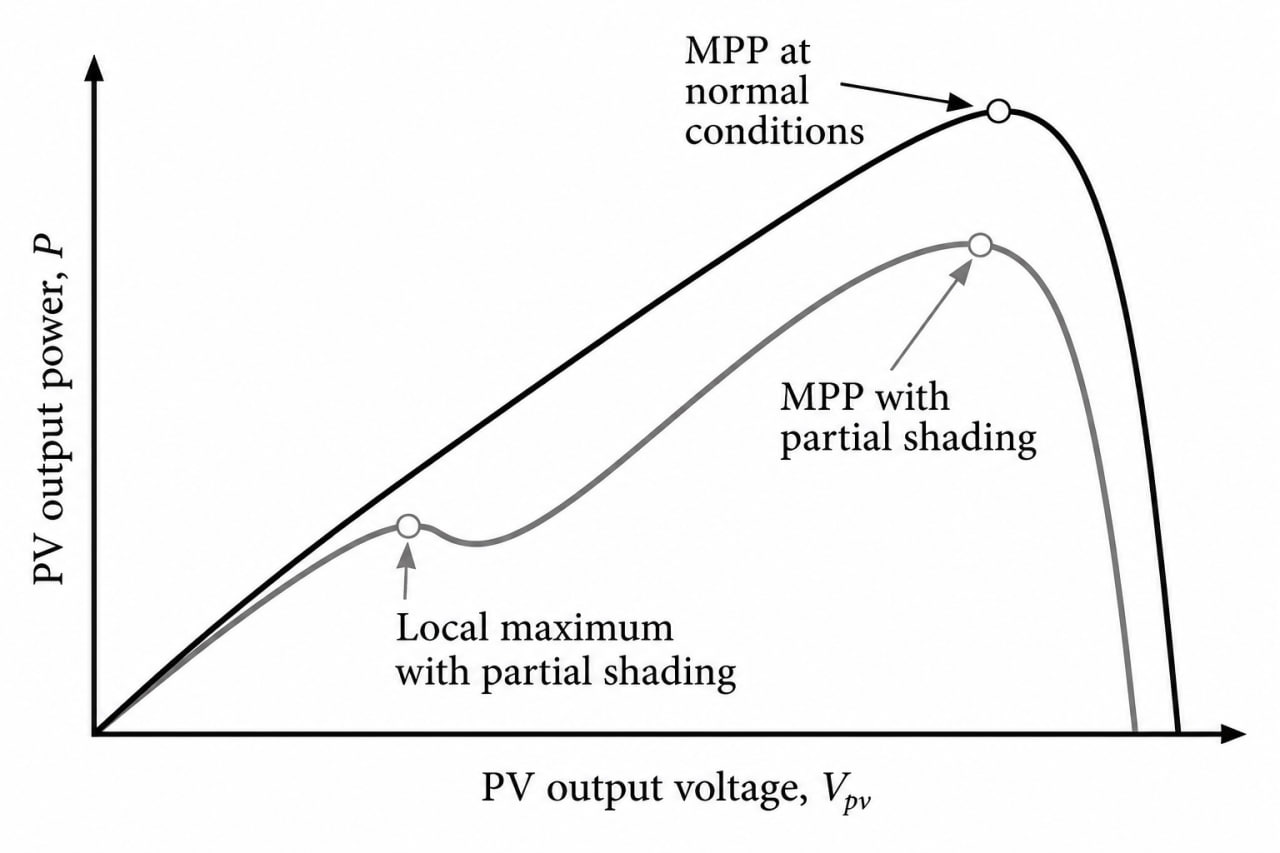
\includegraphics[width=0.7\textwidth]{Figures/Figure 2.19.jpg}
    \caption{Photovoltaic P-V Curve Characteristic Under Partial Shading Conditions.}
    \label{fig:global_vs_local}
\end{figure}

\newpage

\subsection{Advanced Concepts in Engineering Performance}

\subsubsection{Speed vs. Accuracy: Dynamic Efficiency}
In practical photovoltaic applications, atmospheric conditions are rarely static. On overcast days or during rapid cloud movement, solar irradiance can fluctuate drastically within a matter of seconds. This introduces the concept of \textit{Dynamic Efficiency}, which measures the MPPT controller's capability to track rapid variations in solar irradiance, converge on the newly established MPP in the shortest time possible, and maintain system stability without inducing severe oscillations. Balancing fast tracking speed with steady-state tracking accuracy is the absolute core of good engineering design.

\subsubsection{The Cost of Global Scanning (Global Sweep)}
While global scanning techniques are essential to locate the absolute highest peak under partial shading, executing them comes at a distinct energy cost. To search for the Global MPP, the controller must sweep the entire operating range of the PV array, moving from the open-circuit voltage ($V_{oc}$) down to the short-circuit current ($I_{sc}$).

\paragraph{The Engineering Problem:}
During this scanning period (which typically lasts between 1 to 5 seconds depending on the processor speed), the system is forced away from its optimal operating point. Consequently, the output power drops sharply during the sweep.

\paragraph{The Engineering Solution:}
To avoid continuous power layout degradation, the global sweep is not run constantly. Instead, it is programmed at a specific \textit{Periodic Sweep Interval} (e.g., every 10 to 30 minutes). This interval is engineered based on the geographical site conditions and shading patterns, representing a fine engineering trade-off between tracking accuracy and scanning losses.

\subsubsection{Power Conservation and Converter Efficiency}
A common misconception is that an MPPT controller inherently ``creates'' extra electrical energy. In reality, the MPPT operates strictly under the law of conservation of energy using a DC-DC power converter. Assuming an ideal power converter where internal switching losses are neglected, the input power extracted from the solar panels must equal the output power delivered to the load:

\begin{align}
    P_{in} &= P_{out} \\
    V_{in} \times I_{in} &= V_{out} \times I_{out}
\end{align}

\newpage

Based on this fundamental relationship, if the power converter acts to reduce the voltage from $40\text{ V}$ at the input to $20\text{ V}$ at the output, the output current must approximately double to conserve total power:
\begin{equation}
    \text{If } V_{out} = \frac{1}{2}V_{in} \implies I_{out} \approx 2 \times I_{in}
\end{equation}
Therefore, the MPPT does not generate additional power; rather, it dynamically reshapes the voltage-to-current relationship to perfectly match the load demands, optimizing overall system performance.

\subsection{Practical Efficiency and System Limitations}

\subsubsection{Real-World MPPT Efficiency and Loss Mechanisms}
In practical applications, even the most advanced MPPT controllers cannot achieve 100\% efficiency. The power losses within an MPPT system are primarily categorized into:
\begin{itemize}
    \item \textbf{Switching Losses:} Occurring during the high-frequency turn-on and turn-off transitions of power semiconductor switches such as MOSFETs and IGBTs.
    \item \textbf{Core Losses (Eddy Currents):} Occurring within the magnetic cores of inductors and transformers due to alternating magnetic fields.
    \item \textbf{Conduction Losses:} Resulting from the internal DC resistance ($R_{DS(on)}$) of switches, as well as the equivalent series resistance (ESR) of inductors and wiring.
    \item \textbf{Capacitive and Component Mating Losses:} Minor energy dissipation within filtering capacitors and auxiliary electronic components.
\end{itemize}
In modern industrial and commercial systems, the actual efficiency of an MPPT controller ranges between $95\%$ and $99\%$, depending on the power rating, design topology, and real-time operating conditions.

\subsubsection{Practical Constraints and Inverter Clipping}
An MPPT controller does not operate with absolute freedom; it is strictly bounded by the physical and electrical limitations of the power converter:
\begin{itemize}
    \item \textbf{MPPT Voltage Range:} Every tracking device has a specified voltage window (e.g., $150\text{ V}$ to $450\text{ V}$). If environmental factors or temperature fluctuations cause the PV string voltage to drop below the minimum threshold, the controller will completely fail to track the maximum power point.
    \item \textbf{Current Clipping:} Modern ultra-high-power PV modules generate significant current (often $18\text{ A}$ or higher). If the input current exceeds the maximum allowable threshold of the inverter or tracker, the MPPT controller intentionally shifts the operating point toward a higher voltage. This deliberately reduces the current to protect the hardware, resulting in the sacrifice or ``clipping'' of available potential power.
\end{itemize}

\subsection{Control Architecture and Modern Technology Impact}

\subsubsection{The Role of the Closed-Loop Control Architecture}
Inside the digital signal processor (DSP) or microcontroller, the tracking process is managed via a distinct, closed-loop control system. It is functionally divided into two layers:
\begin{itemize}
    \item \textbf{The MPPT Algorithm:} Acts as the high-level decision-maker. It analyzes the $P$-$V$ curve and decides \textit{where} the optimal operating point reference ($V_{ref}$ or $I_{ref}$) should move.
    \item \textbf{The Inner Control Loop:} Acts as the executor. Typically utilizing a Proportional-Integral (PI) or Proportional-Integral-Derivative (PID) digital control technique, it dynamically adjusts the converter's duty cycle ($D$) to drive the system to that reference point smoothly and stably.
\end{itemize}

\subsubsection{Impact of Advanced Photovoltaic Module Technologies}
Modern innovations in solar panel manufacturing directly affect MPPT behavior:
\begin{itemize}
    \item \textbf{Half-Cut Cell Modules:} These modules are split into two parallel, independent sections. When partial shading occurs, the affected half operates independently, drastically reducing the formation of multiple local peaks on the $P$-$V$ curve. This simplifies the tracking process and allows standard MPPT algorithms to operate with higher efficiency.
    \item \textbf{Bifacial Modules:} These panels absorb direct sunlight from the front and reflected ambient light (Albedo) from the rear. Because rear irradiance fluctuates continuously based on surrounding ground conditions, it introduces micro-oscillations into the $P$-$V$ curve, imposing a heavier computational burden on the tracking speed and responsiveness of the MPPT controller.
\end{itemize}

\subsection{Conclusion of MPPT Theory}
In summary, Maximum Power Point Tracking (MPPT) serves as the critical electronic control layer required to overcome the fundamentally non-linear power characteristics of photovoltaic arrays. By dynamically adjusting the duty cycle of an integrated DC-DC power converter, an MPPT system executes continuous impedance matching. This control mechanism ensures that the solar array operates at its peak electrical output regardless of volatile ambient temperatures or shifting solar irradiance levels.
\\

Ultimately, a robustly engineered MPPT control architecture balances tracking speed with steady-state accuracy. This optimization layer is vital for maintaining the high dynamic efficiency and power conservation necessary for demanding infrastructure applications, such as solar-powered electric vehicle charging stations interacting with dynamic DC microgrids.

\chapter{Tools and Equipment}

% =========================================================================
% CHAPTER THREE: TOOLS AND EQUIPMENT USED
% =========================================================================
\section{Introduction}
This chapter describes and presents a comprehensive overview of the tools, the hardware components, measurement instruments, and software tools ``platforms'' that were used and utilized to design, build, test, and operate the solar-powered electric vehicle (EV) charging station. The equipment is categorized according to its functional role within the overall system architecture.

In this chapter, we present the key tools, equipment, and instruments utilized in the process of hardware development, prototyping, testing, and validation of our solar-powered electric vehicle (EV) charging station project. The effective implementation of this project depended not just on correct circuit design and simulation but also on the judicious selection and application of laboratory instruments and measurement systems that guaranteed reliability, repeatability, and safety.

The equipment outlined in this chapter were of paramount importance during several stages of the project, including PCB soldering, component mounting, waveform measurement, and power testing. Each piece of equipment was selected based on its specifications, its suitability to work with power electronics systems, and its ability to enable a smooth workflow throughout the process of assembling and verifying circuits. This chapter describes the technical role played by each device, identifies the reason for inclusion, and defines its particular contribution to the success of the practical implementation of Solar Photovoltaic (PV) Panels, DC-DC converters, and Battery Energy Storage Systems that form the fundamental building blocks of solar-powered electric vehicle (EV) charging station system.

% =========================================================================
% SECTION 3.2: POWER SUPPLY & DISTRIBUTION DEVICES
% =========================================================================
\section{Power Supply \& Distribution Devices}

\subsection{Programmable DC Power Supply (TDK-Lambda GEN 300-11)}

\subsubsection{Tool Overview}
The TDK-Lambda GEN 300-11 is a programmable DC power supply from the GENESYS\texttrademark\ series, known for its high performance, reliability, and precision in laboratory and industrial environments. This specific model provides an output range of 0--300 V DC and up to 11 A of output current, making it suitable for medium to high-power applications in power electronics testing. The unit supports both manual control via its front panel and remote control through analog or digital interfaces such as RS-232, GPIB, or LAN. Its front panel allows precise voltage and current adjustment using rotary encoders, as well as monitoring via digital display.

\begin{figure}[H]
    \centering
    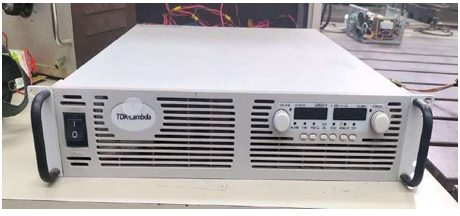
\includegraphics[width=0.75\textwidth]{Figures/Figure 3.1.png}
    \caption{TDK-Lambda GEN 300-11 Programmable DC Power Supply.}
    \label{fig:tdk_lambda}
\end{figure}

\subsubsection{Key Specifications}
\renewcommand{\arraystretch}{1.3}
\rowcolors{2}{white}{gray!8}
\begin{tabularx}{\textwidth}{>{\bfseries}X l}
    \toprule
    Parameter & Specification \\
    \midrule
    Model & TDK-Lambda GEN 300-11 \\
    O/P Voltage Range & 0--300 V DC \\
    O/P Current Range & 0--11 A \\
    Power Output & Up to 3.3 kW \\
    Interface & Local + Remote (RS-232, GPIB, LAN) \\
    Protection Features & Overvoltage, Overcurrent, Foldback, Overtemperature \\
    \bottomrule
\end{tabularx}

\subsubsection{Role in the Graduation Project}
This programmable DC power supply was a critical component in the hardware validation of the solar-powered electric vehicle (EV) charging station circuits. Its ability to provide a precisely regulated and adjustable DC voltage allowed for the safe and repeatable powering of various converter topologies implemented during the project.

Specifically, it was used to:
\begin{itemize}
    \item Power the DC-DC converter circuits (Buck, Boost, Buck-Boost) under controlled conditions.
    \item Test different duty cycles and load conditions by adjusting input voltage dynamically.
    \item Ensure stable and isolated DC input, mimicking real-world conditions without the hazards of using high-voltage batteries during early testing phases.
\end{itemize}

% =========================================================================
% SECTION 3.3: MEASUREMENT & MONITORING INSTRUMENTS
% =========================================================================
\section{Measurement \& Monitoring Instruments}

\subsection{Digital Storage Oscilloscope - Hantek DSO4254B}

\subsubsection{Tool Overview}
The Hantek DSO4254B is a 4-channel Digital Storage Oscilloscope (DSO) widely used in electrical engineering laboratories for capturing, visualizing, and analyzing electrical waveforms. With a bandwidth of 250 MHz and a real-time sampling rate of up to 1 GSa/s, it is suitable for diagnosing both low- and high-frequency signals in power electronics applications. This oscilloscope offers precise control over vertical and horizontal axes, trigger settings, and math operations, making it highly adaptable for testing converters, inverters, and complex switching circuits like those found in solar-powered electric vehicle (EV) charging stations.

\begin{figure}[H]
    \centering
    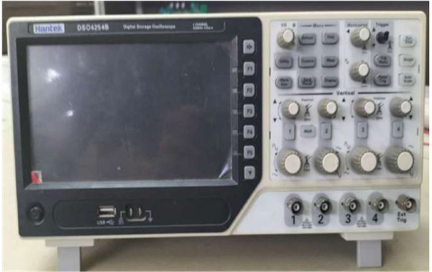
\includegraphics[width=0.7\textwidth]{Figures/Figure 3.2.png}
    \caption{Hantek DSO4254B Digital Storage Oscilloscope.}
    \label{fig:hantek_oscilloscope}
\end{figure}

\subsubsection{Key Specifications}
\renewcommand{\arraystretch}{1.4} % Slightly more breathing room
\rowcolors{2}{white}{gray!8} 

\begin{tabularx}{\textwidth}{>{\bfseries}l X} % <-- Changed first to 'l' and second to 'X'
    \toprule
    Parameter & Specification \\
    \midrule
    Model & Hantek DSO4254B \\
    Channels & 4 (CH1--CH4) + External Trigger (Ext Trig) \\
    Bandwidth & 250 MHz \\
    Real-time Sampling Rate & 1 GSa/s \\
    Display & Large color LCD screen \\
    Ports & USB Host, USB Device, LAN \\
    Functions & Waveform generator, cursor measurements, auto-set, FFT analysis, save/recall \\
    \bottomrule
\end{tabularx}

\subsubsection{Role in the Graduation Project}
This oscilloscope was indispensable in verifying the performance and stability of the entire power conversion system used in the solar-powered electric vehicle (EV) charging station. It provided real-time, high-resolution visibility into the behavior of voltage and current waveforms across different stages of the circuit, including:
\begin{itemize}
    \item DC-DC converter output ripple measurements and transient response.
    \item Switching behavior analysis for MOSFETs and IGBTs in the Buck, Boost, and Buck-Boost circuits.
    \item Gate signal validation from the control circuit and drivers.
    \item Startup and shutdown transients during power sequencing tests.
\end{itemize}
The ability to visualize waveform distortion, harmonics, and frequency behavior was essential for matching simulation results from MATLAB/Simulink with physical circuit behavior, ensuring accurate hardware validation.

\subsubsection{Importance in Achieving Project Goals}
Without this oscilloscope, it would not have been possible to:
\begin{itemize}
    \item Confirm switching frequency adherence and waveform shape.
    \item Validate converter efficiency by analyzing voltage/current overlap.
    \item Identify noise or instability issues in real time.
    \item Troubleshoot signal integrity during integration between stages.
\end{itemize}

\subsection{Oscilloscope - DSO 138}
\subsubsection{Tool Overview}
It was very practical for home testing when the laboratory was not reachable.
\begin{figure}[H]
    \centering
    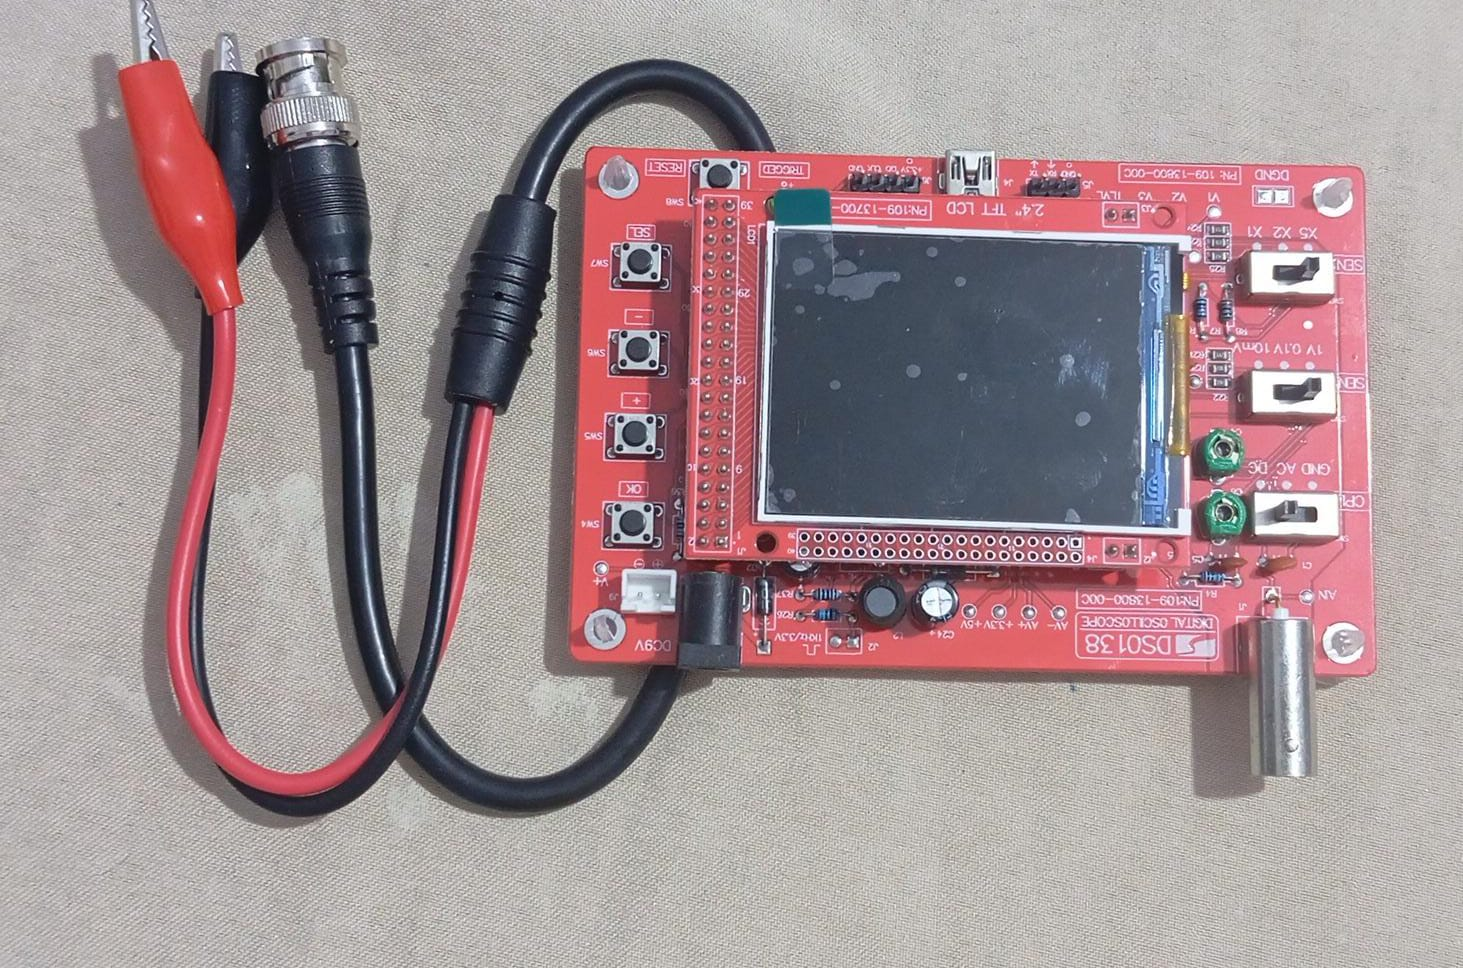
\includegraphics[width=0.7\textwidth]{Figures/Figure 3.3.jpeg}
    \caption{DSO 138 Oscilliscope}
    \label{fig:multimeter}
\end{figure}


% -------------------------------------------------------------------------
\subsection{Digital Multimeter - UNI-T UT33D+}

\subsubsection{Description}
The UNI-T UT33D+ is a handheld digital multimeter used for measuring a variety of electrical parameters. It is part of the UT33+ series, known for affordability and reliability in lab and educational settings. This particular model supports both AC and DC voltage, current, resistance, diode testing, and continuity checking, and includes a non-contact voltage (NCV) detection function for live wire sensing.

\begin{figure}[H]
    \centering
    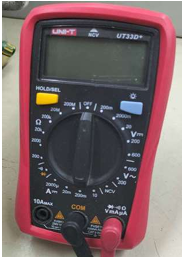
\includegraphics[width=0.35\textwidth]{Figures/Figure 3.4.png}
    \caption{UNI-T UT33D+ Digital Multimeter.}
    \label{fig:multimeteer}
\end{figure}

\subsubsection{Key Features}
\renewcommand{\arraystretch}{1.4} % Nice breathing room between rows
\rowcolors{2}{white}{gray!8} % Alternating soft gray zebra stripes

\begin{tabularx}{\textwidth}{>{\bfseries}l X}
    \toprule
    Feature Category & Technical Specification \\
    \midrule
    Voltage Measurement & AC/DC Voltage up to 600 V \\
    Current Measurement & DC Current up to 10 A (utilizing the dedicated 10A MAX port) \\
    Resistance Measurement & Resistance range up to 20 M$\Omega$ \\
    Testing Functions & Integrated diode testing and circuit continuity checking \\
    Safety \& Convenience & Non-Contact Voltage (NCV) detection, manual range selection, display hold function, backlit display, and fused inputs (250V/200mA and 250V/10A) \\
    \bottomrule
\end{tabularx}

\newpage

% -------------------------------------------------------------------------
\subsection{Voltage Sensor Module – DC 0-25V}

\subsubsection{Description}
The voltage sensor module is a compact board based on a resistive voltage divider, used to scale down DC voltages so they can be safely read by a microcontroller's analog input. Since the Arduino's analog pins can only accept up to 5V, this module allows voltages as high as 25V to be measured indirectly by reducing the input by a fixed factor before it reaches the analog pin.

\begin{figure}[H]
    \centering
    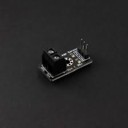
\includegraphics[width=0.45\textwidth]{Figures/Figure 3.5.jpg}
    \caption{DC 0--25V Voltage Sensor Module.}
    \label{fig:voltage_sensor}
\end{figure}

\subsubsection{Key Specifications}
\renewcommand{\arraystretch}{1.4} % Nice breathing room between rows
\rowcolors{2}{white}{gray!8} % Alternating soft gray zebra stripes

\begin{tabularx}{\textwidth}{>{\bfseries}l X}
    \toprule
    Parameter & Specification \\
    \midrule
    Type & Resistive Voltage Divider Sensor Module \\
    Voltage Input Range & DC 0--25 V \\
    Divider Ratio & 5:1 \\
    Divider Resistors & 30 k$\Omega$ and 7.5 k$\Omega$, 1\% tolerance \\
    Voltage Detection Resolution & 0.00489 V \\
    Key Function & Scales down higher DC voltages to a safe 0--5V range for analog measurement by a microcontroller \\
    \bottomrule
\end{tabularx}

\newpage

\subsubsection{Application in the Project}
In this project, the voltage sensor module is used to measure DC voltage at key points in the circuit, such as the PV array output and battery terminal voltage, by scaling the measured voltage down by a factor of 5 before feeding it into the Arduino Uno's analog input. This scaled voltage reading allows the Arduino to reconstruct the actual voltage value in software and use it, alongside the ACS712 current sensor reading, for the MPPT algorithm's power calculation and duty-cycle adjustment, as well as for monitoring battery voltage during charge/discharge control.

% -------------------------------------------------------------------------
\subsection{Current Sensor – ACS712 (5A)}

\subsubsection{Description}
The ACS712 is a fully integrated, Hall-effect-based linear current sensor IC that measures both AC and DC current and converts it into a proportional analog voltage output. Since it senses current through a magnetic field rather than a direct electrical connection, it provides galvanic isolation between the high-current path being measured and the low-voltage signal/control circuitry, making it safe to interface directly with a microcontroller's analog input.

\begin{figure}[H]
    \centering
    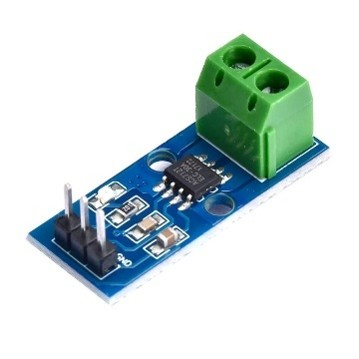
\includegraphics[width=0.45\textwidth]{Figures/Figure 3.6.jpg}
    \caption{ACS712 5A Current Sensor Module.}
    \label{fig:current_sensor}
\end{figure}

\subsubsection{Key Specifications}
\renewcommand{\arraystretch}{1.4} % Nice breathing room between rows
\rowcolors{2}{white}{gray!8} % Alternating soft gray zebra stripes

\begin{tabularx}{\textwidth}{>{\bfseries}l X}
    \toprule
    Parameter & Specification \\
    \midrule
    Manufacturer & Allegro MicroSystems \\
    Type & Hall-Effect Linear Current Sensor IC (module/breakout board) \\
    Model & ACS712ELC-05A (5A variant) \\
    Measurement Range & $-5$ A to $+5$ A (bidirectional) \\
    Sensitivity & 180--190 mV/A, typically 185 mV/A \\
    Supply Voltage & 4.5 V to 5.5 V DC \\
    Zero-Current Output Voltage & $V_{CC}/2$ (2.5 V at 5V supply) \\
    Isolation & 2.4 kV$_{RMS}$ isolation \\
    Key Function & Converts measured DC/AC current into a proportional analog voltage signal for monitoring or feedback control \\
    \bottomrule
\end{tabularx}

\subsubsection{Application in the Project}
In this project, the ACS712 5A current sensor measures current at key points—such as PV array output and battery charge/discharge current—and feeds the corresponding analog voltage signal to the Arduino's analog input. This current feedback is essential to the MPPT algorithm, which uses it alongside voltage readings to calculate PV power and adjust the duty cycle accordingly, and also supports safe charge/discharge current regulation for the battery.

% =========================================================================
% SECTION 3.4: LOAD SIMULATION DEVICES (BATTERIES)
% =========================================================================
\section{Load Simulation Devices (Batteries)}

\subsection{EV Battery Simulator (IMR14500 Lithium-Ion Pack)}

\subsubsection{Description}
The battery used to simulate the electric vehicle in this project consists of two IMR14500 lithium-ion cells, each rated 3.7V 800mAh, connected in series to form a 7.4V nominal pack. The IMR14500 is a rechargeable lithium-manganese cell in the AA-size (14500) format, designed for stable power delivery, fast charging, and long cycle life, making it suitable as a compact, scaled-down stand-in for an EV battery in laboratory testing.

\begin{figure}[H]
    \centering
    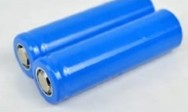
\includegraphics[width=0.6\textwidth]{Figures/Figure 3.7.jpg}
    \caption{Lithium-Ion Battery Pack (IMR14500 Cells in 2S Configuration).}
    \label{fig:ev_battery_pack}
\end{figure}

\subsubsection{Key Specifications}
\renewcommand{\arraystretch}{1.4} % Provides clean vertical padding
\rowcolors{2}{white}{gray!8} % Alternating soft gray zebra stripes

\begin{tabularx}{\textwidth}{>{\bfseries}l X}
    \toprule
    Parameter & Specification \\
    \midrule
    Cell Type & IMR14500 Lithium-Ion (Lithium-Manganese chemistry) \\
    Cell Size & 14500 (AA-size format) \\
    Nominal Voltage per Cell & 3.7 V \\
    Capacity per Cell & 800 mAh (actual capacity) \\
    Configuration & 2 cells in series (2S) \\
    Nominal Pack Voltage & 7.4 V \\
    Pack Capacity & 800 mAh (capacity unchanged in series connection; only voltage adds) \\
    Charge Cut-off Voltage & Typically 4.2 V per cell (pack total: 8.4 V) \\
    Discharge Cut-off Voltage & Typically 3.0 V per cell (pack total: 6.0 V) \\
    Key Function & Acts as a scaled-down model of an electric vehicle battery for laboratory testing \\
    \bottomrule
\end{tabularx}

\subsubsection{Application in the Project}
In this project, the 2S IMR14500 3.7V 800mAh lithium-ion battery pack is used to simulate an electric vehicle's battery during laboratory testing, representing the load to be charged by the PV-based charging station. This allows the charging behavior of the system—including the converter stages and control algorithm—to be validated on a small scale, safely standing in for an actual EV battery pack.

% -------------------------------------------------------------------------
\subsection{Stationary Battery Storage System (ICR18650 Pack with BMS)}

\subsubsection{Description}
The energy storage battery used in this project (for storing PV energy when no EV is connected) consists of two ICR18650 lithium-ion cells connected in series, paired with an HW-391 battery management system (BMS) protection board. The BMS monitors and protects the cell pack during charge and discharge, preventing overcharge, over-discharge, and overcurrent conditions that could otherwise damage the cells or create safety hazards.

\begin{figure}[H]
    \centering
    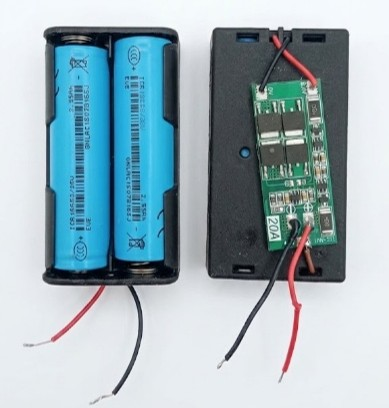
\includegraphics[width=0.35\textwidth]{Figures/Figure 3.8.jpg}
    \caption{ICR18650 Battery Storage Pack with Integrated Protection Board Layout.}
    \label{fig:storage_battery_pack}
\end{figure}

\subsubsection{Key Specifications}
\renewcommand{\arraystretch}{1.3}
\rowcolors{2}{white}{gray!8}
\begin{tabularx}{\textwidth}{X X}
    \toprule
    \textbf{Battery Cells Component} & \textbf{BMS Protection Board (HW-391)} \\
    \midrule
    Manufacturer: EVE Energy & Model: HW-391 \\
    Cell Type: ICR18650 Lithium-Ion (18650 cylindrical format) & Configuration: 2S Li-ion protection board \\
    Nominal Voltage per Cell: 3.7 V & Maximum Discharge Current: 20 A \\
    Capacity per Cell: 2.55 Ah (2550 mAh) & Charge Cut-off Voltage: 8.4 V (4.2 V per cell) \\
    Configuration: 2 cells in series (2S) & Discharge Cut-off Voltage: $\sim$6.0 V (3.0 V per cell) \\
    Nominal Pack Voltage: 7.4 V & Key Function: Overcharge, over-discharge, and \\
    Pack Capacity: 2.55 Ah & overcurrent protection for the 2S battery pack \\
    \bottomrule
\end{tabularx}

\newpage

\subsubsection{Application in the Project}
In this project, this 2S ICR18650 battery pack (with integrated BMS) serves as the system's energy storage element, used when no simulated EV is connected to the charging station. It stores excess energy harvested from the PV array through the MPPT-controlled converter stage, allowing the system to continue supplying power when solar generation is intermittent or unavailable. The HW-391 BMS protects the pack during both charging from the PV side and discharging to the load, ensuring the cells operate within safe voltage and current limits throughout testing.

% =========================================================================
% SECTION 3.5: CONTROL DEVICES
% =========================================================================
\section{Control Devices}

\subsection{Arduino Uno Development Board}

\subsubsection{Description}
\begin{itemize}
    \item \textbf{Manufacturer / Series:} Arduino AG / Arduino LLC (Arduino Uno Rev3).
    \item \textbf{Core Processing Hardware:} ATmega328P micro-controller utilizing an 8-bit AVR RISC architecture operating at a clock speed of 16 MHz.
    \item \textbf{Onboard Features:} 14 digital I/O pins (6 of which provide PWM output), 6 analog input pins, and 1 UART (hardware serial) port.
    \item \textbf{Power Options \& Connectivity:} Supports USB programming/communication (5V interface) or external power via DC jack / $V_{in}$ pin ($7$--$12\text{V}$ recommended), equipped with an onboard voltage regulator, reset button, SPI, and $\text{I}^2\text{C}$ interfaces.
\end{itemize}

\begin{figure}[H]
    \centering
    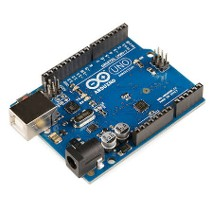
\includegraphics[width=0.5\textwidth]{Figures/Figure 3.9.jpg}
    \caption{Arduino Uno Rev3 Development Board.}
    \label{fig:arduino_uno}
\end{figure}

\subsubsection{Application in the Project}
In this project, the Arduino Uno serves as the central digital controller responsible for generating the switching signals for the power electronic stages in the solar-to-EV-charging system. Since the Uno's PWM outputs are low-power logic-level signals (0--5V), they are not capable of directly driving the power semiconductor switches; therefore, external gate driver ICs are used to amplify and level-shift these signals to the voltage/current levels required to switch the MOSFETs/IGBTs in each converter stage.

\begin{description}
    \item[MPPT Control:] The Arduino reads the PV array's voltage and current through its analog input channels (via voltage/current sensor signals) and runs the Maximum Power Point Tracking algorithm (e.g., Perturb \& Observe or Incremental Conductance) in real time. Based on the computed reference, it generates a PWM duty cycle signal, which is fed through a gate driver IC to drive the MPPT-stage DC-DC converter switch, continuously adjusting the duty cycle to keep the PV array operating at its maximum power point under varying irradiance and temperature.
    \item[Boost Converter Control:] A PWM output channel from the Arduino is passed through a gate driver IC to drive the boost converter switch, regulating the step-up of PV output voltage to the level required by the battery bus or DC link.
    \item[Buck Converter Control:] Another PWM channel, similarly buffered through a gate driver IC, controls the buck converter switching, stepping down the bus voltage to the level required for battery charging or for the EV charging output.
    \item[Two-Quadrant Chopper Control:] The Arduino generates the gating signals for the two-quadrant (bidirectional) chopper; these are routed through dedicated gate driver ICs to drive both switches of the chopper, enabling controlled power flow in both directions—allowing the system to manage battery charging (buck mode) and discharging/power delivery (boost mode) depending on system state.
    \item[Signal Conditioning Interface:] Voltage and current sensor outputs are fed into the Arduino's analog inputs (after appropriate scaling/conditioning circuitry) to enable closed-loop feedback control across all converter stages.
    \item[Gate Driver Interface:] The gate driver ICs serve as the isolation and amplification stage between the Arduino's low-voltage logic outputs and the high-voltage/high-current switching requirements of the power converters, also providing protection against noise and voltage spikes from the power circuit reaching the microcontroller.
\end{description}

% =========================================================================
% SECTION 3.6: BASIC POWER ELECTRONICS COMPONENTS
% =========================================================================
\section{Basic Power Electronics Components}

\subsection{IR2111 – High-Voltage Gate Driver IC}

\subsubsection{Description and Key Specifications}
The IR2111 is a high-voltage, high-speed half-bridge gate driver IC designed to level-shift and amplify low-power logic signals into high-current gate drive signals for high-side and low-side power MOSFETs or IGBTs.

\begin{figure}[H]
    \centering
    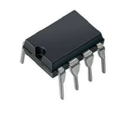
\includegraphics[width=0.2\textwidth]{Figures/Figure 3.10.png}
    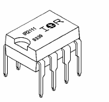
\includegraphics[width=0.17\textwidth]{Figures/Figure 3.11.png}
    \caption{High-Voltage Half-Bridge Gate Driver IC IR2111 Block Assignment.}
    \label{fig:gate_driver_ic}
\end{figure}

\renewcommand{\arraystretch}{1.4} % Provides clean vertical padding
\rowcolors{2}{white}{gray!8} % Alternating soft gray zebra stripes

\noindent % Prevents any accidental paragraph indentation shifts
\centerline{% Forces the entire text-width container into exact center alignment
\begin{tabularx}{\textwidth}{>{\bfseries}l X}
    \toprule
    Parameter & Specification \\
    \midrule
    Manufacturer & International Rectifier (now Infineon Technologies) \\
    Voltage Ratings & Operates up to $+600$ V with a high-side floating channel supply \\
    Output Current Capability & $0.5$ A sink and $0.25$ A source (typical values) \\
    Logic Compatibility & Logic input voltage is compatible with standard TTL/CMOS levels (0 V to $V_{CC}$), independent of the high-voltage supply rail channel \\
    Propagation Delay Parameters & Features a turn-on propagation delay of 750 ns and a turn-off propagation delay of 150 ns \\
    \bottomrule
\end{tabularx}%
}

\subsubsection{Application in the Project}
In this project, the IR2111 interfaces between the Arduino Uno's low-voltage PWM outputs and the IRFP260 MOSFETs used in the boost converter, buck converter, and two-quadrant chopper. Since the Arduino cannot supply enough current to switch the MOSFETs quickly, the IR2111 amplifies and level-shifts each PWM signal to drive the gates with fast, clean transitions and minimal switching loss. 

Its independent high-side and low-side channels, with built-in dead-time protection, make it especially suited to the two-quadrant chopper, where both switches must operate without overlap to avoid short-circuiting the DC bus. The floating high-side channel also allows proper switching even when the high-side MOSFET's source is not grounded.

% -------------------------------------------------------------------------
\subsection{Optocoupler – 6N139}

\subsubsection{Description and Key Specifications}
The 6N139 is a high-gain, split-Darlington output optocoupler designed to provide safe electrical isolation between low-voltage control circuits and high-voltage power electronic stages.

\begin{figure}[H]
    \centering
    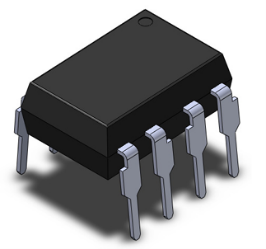
\includegraphics[width=0.2\textwidth]{Figures/Figure 3.12.png}
    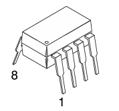
\includegraphics[width=0.2\textwidth]{Figures/Figure 3.13.png}
    \caption{6N139 High-Gain Darlington Optocoupler Package.}
    \label{fig:optocoupler}
\end{figure}

\begin{itemize}
    \item \textbf{Output Type:} Split-Darlington Transistor (provides an exceptionally high Current Transfer Ratio - CTR, typically exceeding 400\%).
    \item \textbf{Switching Capability:} Suitable for PWM frequencies in the low tens of kilohertz range (e.g., 10 kHz) when appropriately calibrated with a dynamic pull-down resistor.
    \item \textbf{Input Forward Voltage:} 1.4 V typical threshold.
    \item \textbf{Isolation Rating:} Up to $5000\text{ V}_{RMS}$ high galvanic isolation.
\end{itemize}

\subsubsection{Application in the Project}
In this project, the 6N139 optocoupler is placed between the Arduino Uno's PWM output and the input of the IR2111 gate driver IC, serving across various converter control channels (MPPT stage, boost converter, buck converter, and two-quadrant chopper). Its primary role is to \textit{electrically isolate the low-voltage microcontroller side from the high-voltage power electronics side}, since the gate driver and MOSFETs operate at higher voltage and current levels and are directly exposed to severe switching noise, ground bounce, and potential fault conditions.

The exceptionally high CTR of the 6N139's Darlington stage is critical for this application, as it allows the weak, milliampere-level 5V logic signal from the Arduino to deeply saturate the output transistor and robustly trigger the 12V gate drive stage. Furthermore, due to the specific pull-down wiring configuration utilized in the hardware, the 6N139 inherently acts as a logical inverter (a HIGH signal from the microcontroller pulls the isolated output LOW). This precise hardware behavior is actively compensated for within the embedded control firmware to maintain accurate duty-cycle regulation without introducing latency, preserving the responsiveness of the MPPT algorithm and the converter closed-loop control.
\newpage
% -------------------------------------------------------------------------
\subsection{MOSFET – IRFP260N}

\subsubsection{Description and Key Specifications}
The IRFP260N is an advanced N-channel power MOSFET utilizing HEXFET® technology, specifically optimized for high-speed, heavy-duty power switching applications requiring extremely low conduction losses.

\begin{figure}[H]
    \centering
    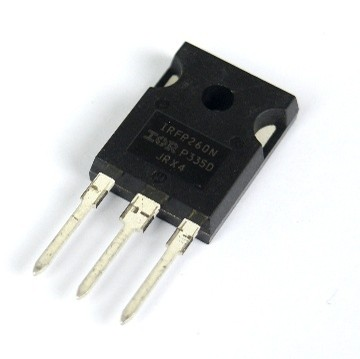
\includegraphics[width=0.2\textwidth]{Figures/3.14.jpg}
    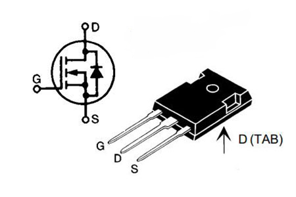
\includegraphics[width=0.35\textwidth]{Figures/3.144.png}
    \caption{IRFP260N Power MOSFET Schematic Symbol and TO-247AC Package Outline.}
    \label{fig:mosfet}
\end{figure}

\renewcommand{\arraystretch}{1.4} % Provides clean vertical padding
\rowcolors{2}{white}{gray!8} % Alternating soft gray zebra stripes

\noindent % Prevents any accidental paragraph indentation shifts
\centerline{% Forces the entire text-width container into exact center alignment
\begin{tabularx}{\textwidth}{>{\bfseries}l X}
    \toprule
    Parameter & Specification \\
    \midrule
    Manufacturer & Infineon Technologies / International Rectifier (IR) \\
    Drain-Source Breakdown Voltage ($V_{DS}$) & 200 V \\
    Continuous Drain Current ($I_D$) & 50 A (at $T_c = 25^\circ\text{C}$) \\
    On-State Channel Resistance ($R_{DS(on)}$) & $0.04\ \Omega$ at $V_{GS} = 10\text{ V}$ \\
    Gate Threshold Voltage Range & 2.0 V to 4.0 V \\
    \bottomrule
\end{tabularx}%
}

\subsubsection{Application in the Project}
The IRFP260N serves as the primary switching semiconductor in the bidirectional Two-Quadrant Chopper, as well as the independent boost and buck converter stages. Driven by the isolated IR2111 gate driver IC, it switches ON and OFF precisely at the 10 kHz duty cycle commanded by the microcontroller to regulate the microgrid's energy transfer. 

The selection of the "N" variant is critical to the system's thermodynamic stability. Its robust 200V/50A ratings provide an absolute safety margin against transient inductive spikes ($V = L \frac{di}{dt}$). More importantly, its ultra-low on-state resistance ($R_{DS(on)} = 0.04\ \Omega$) is the cornerstone of the Synchronous Rectification strategy utilized in the Two-Quadrant Chopper. By substituting standard freewheeling diodes with this actively driven MOSFET, conduction losses are drastically minimized, transitioning the thermal dissipation from a linear function to a quadratic resistive function. Coupled with the large TO-247AC package, this allows the power stages to operate efficiently under continuous 0.40A to high-current off-grid loads without necessitating complex forced-air cooling infrastructure.
\newpage
% -----------------------------------------
\subsection{Resistors}

\subsubsection{Description and Key Specifications}
Resistors are passive components used to limit current, divide voltage, and bias active components. In this project, resistors of different values and power ratings were used across the circuit—from low-power signal applications, like gate driver and optocoupler inputs, to higher-power applications, like voltage sensing and current limiting in the power stages.

\begin{figure}[H]
    \centering
    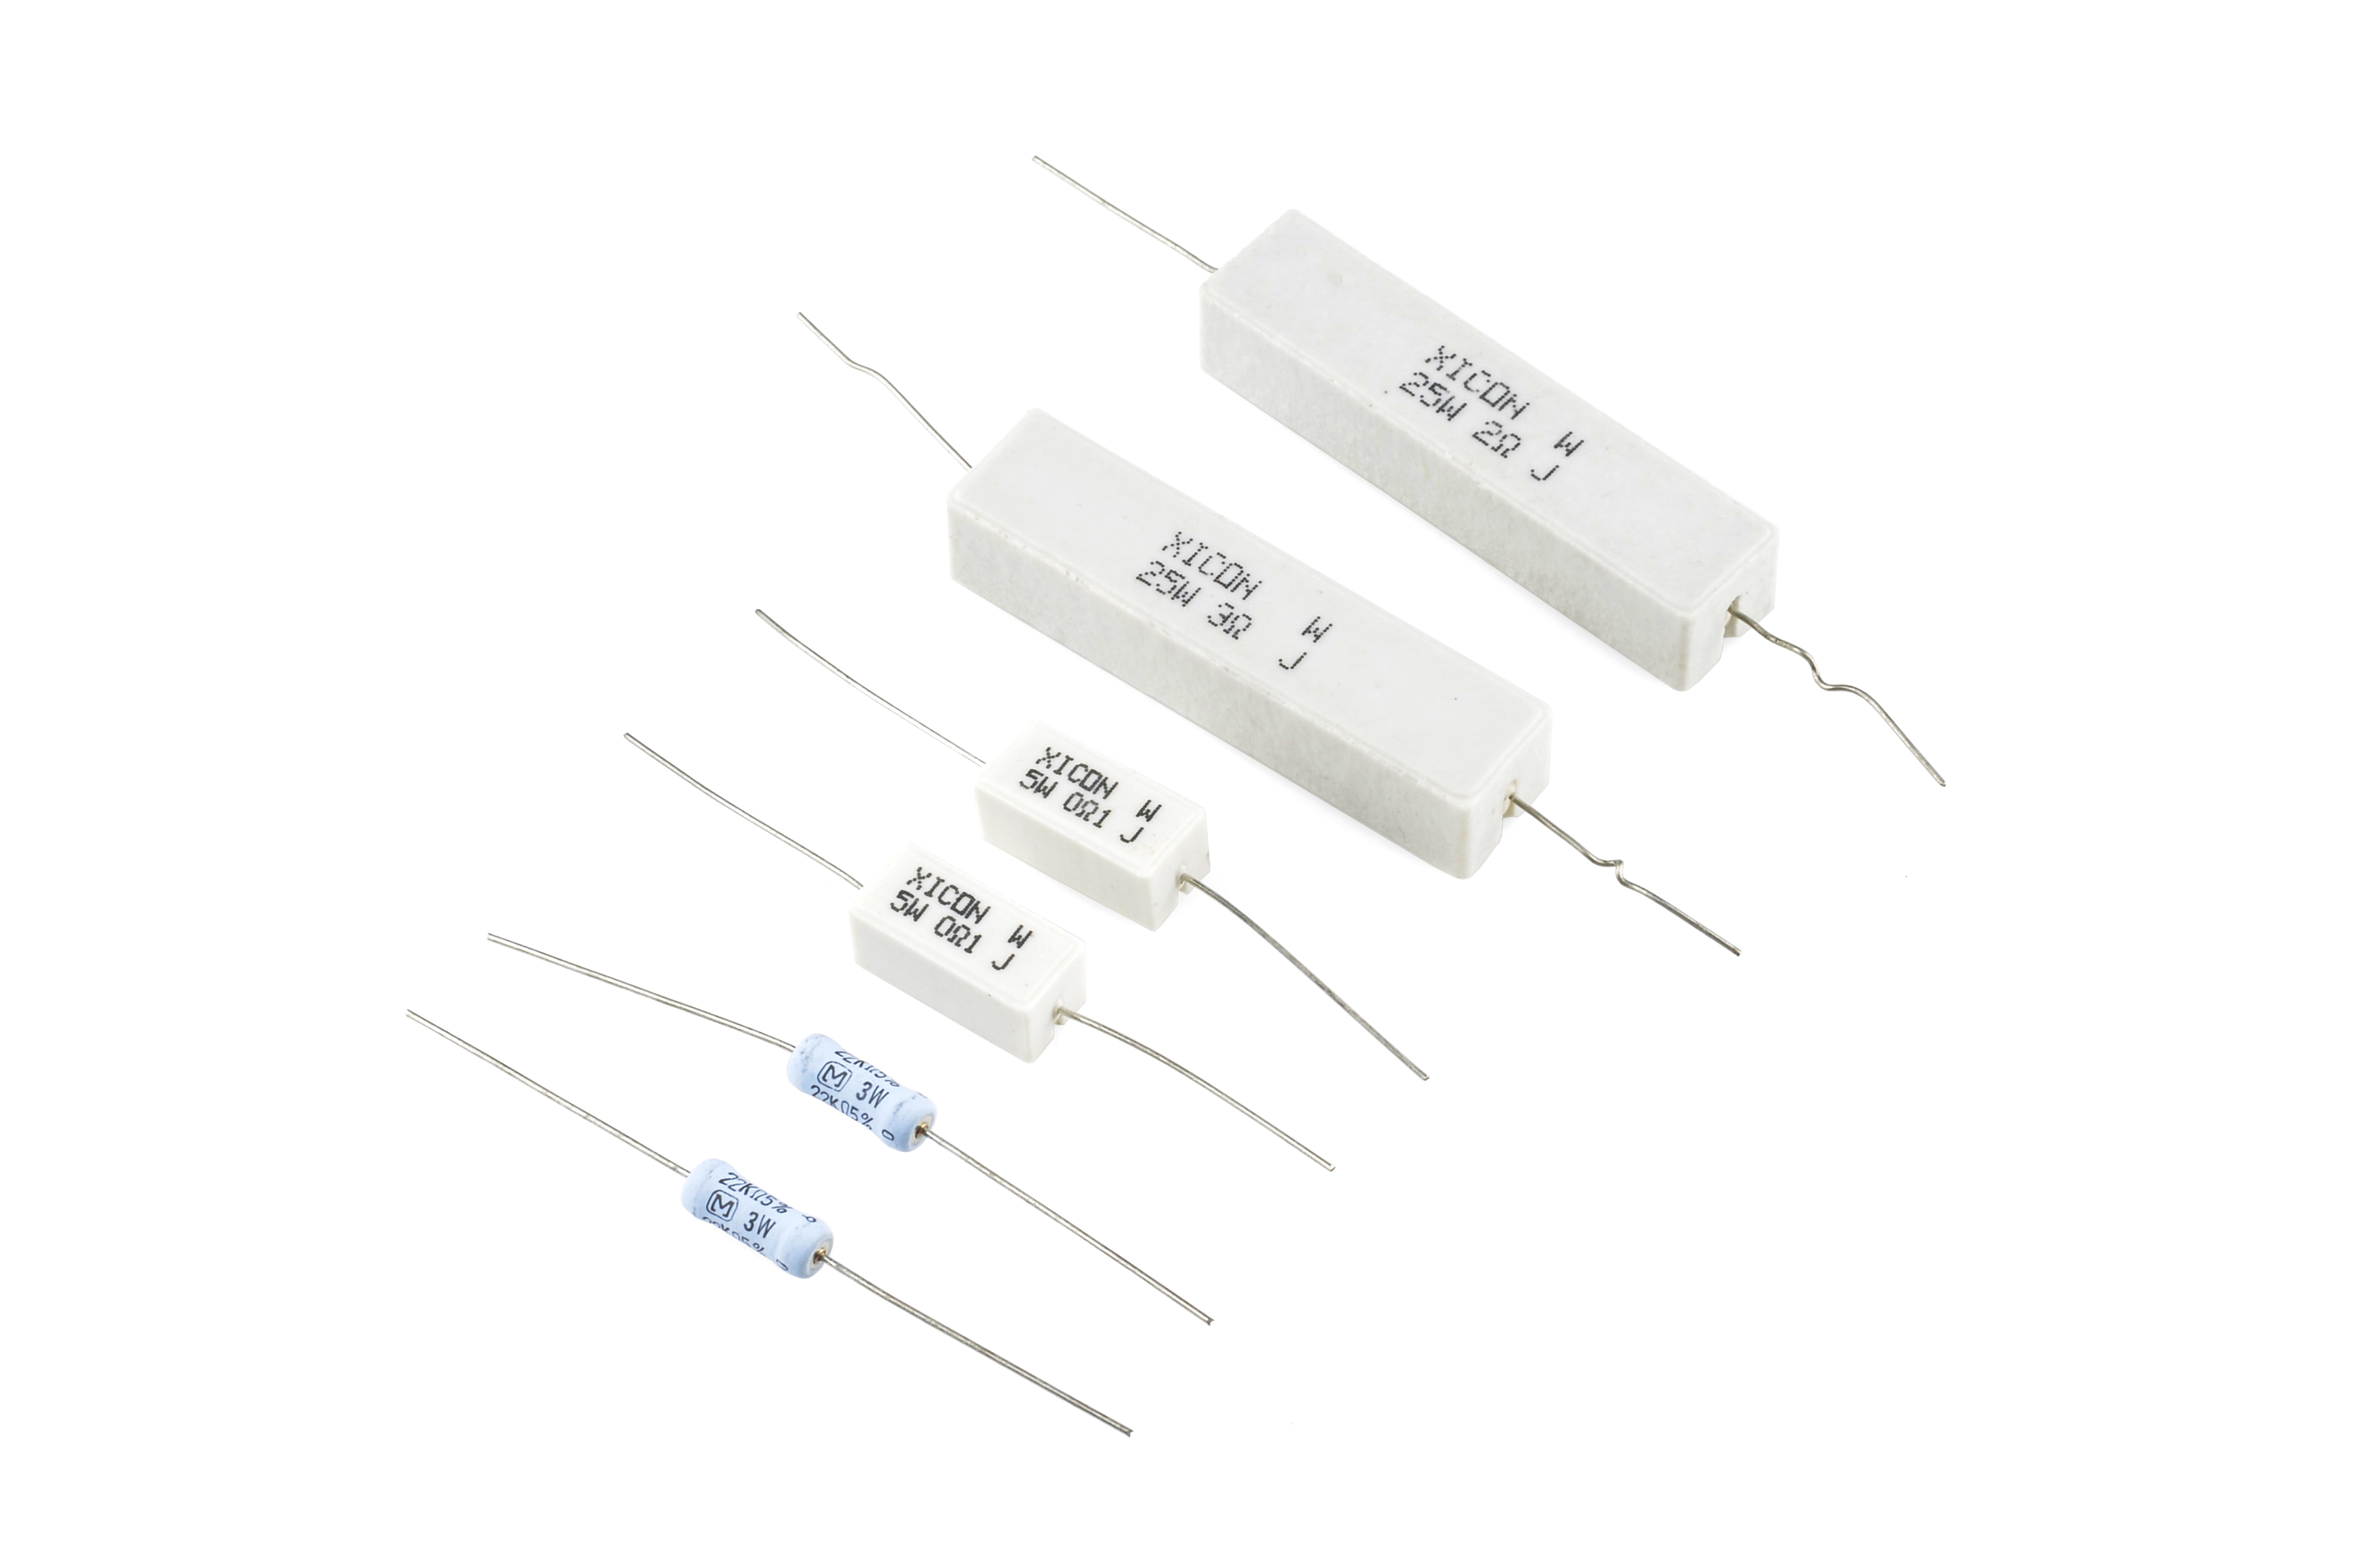
\includegraphics[width=0.4\textwidth]{Figures/res.jpg}
    \caption{Through-Hole Fixed Resistor Component Structure.}
    \label{fig:resistor}
\end{figure}

\renewcommand{\arraystretch}{1.4} % Provides clean vertical padding
\rowcolors{2}{white}{gray!8} % Alternating soft gray zebra stripes

\noindent % Prevents any accidental paragraph indentation shifts
\centerline{% Forces the entire text-width container into exact center alignment
\begin{tabularx}{\textwidth}{>{\bfseries}l X}
    \toprule
    Parameter & Specification \\
    \midrule
    Type & Fixed carbon-film / metal-film resistors (through-hole parameters) \\
    Resistance Values & Multiple values used (ranging from a few ohms up to several kilo-ohms), selected per circuit requirement \\
    Power Ratings & Multiple ratings used (1/4 W for signal-level circuits up to several watts for higher-current sections), selected based on expected power dissipation at each location \\
    Tolerance Value & $\pm5\%$ standard margin for general-purpose applications \\
    \bottomrule
\end{tabularx}%
}

\subsubsection{Application in the Project}
In this project, resistors were used in several roles depending on the circuit stage:
\begin{itemize}
    \item \textbf{Pull-up/Pull-down and Biasing:} Used at the inputs/outputs of the optocoupler (6N137M) and gate driver IC (IR2111) to ensure proper logic-level operation and prevent floating signals.
    \item \textbf{Voltage Division:} Used in sensing circuits to scale down higher voltages (e.g., PV array or battery voltage) to levels safely readable by the Arduino's analog input pins.
    \item \textbf{Current Limiting:} Used to protect LEDs, optocoupler input diodes, and other low-power components from excessive current.
    \item \textbf{Current Sensing:} Higher-power resistors (shunt-type) were used where applicable to sense current flow in the power stages, generating a small voltage drop proportional to current for feedback purposes.
\end{itemize}

% -------------------------------------------------------------------------
\subsection{Inductors}

\subsubsection{Description and Key Specifications}
Power inductors are passive components used to store energy in a magnetic field and smooth current flow. In this project, power inductors of different inductance values and current ratings were used as the main energy-storage elements in the boost converter, buck converter, and two-quadrant chopper.

\begin{figure}[H]
    \centering
    \begin{minipage}{0.48\textwidth}
        \centering
        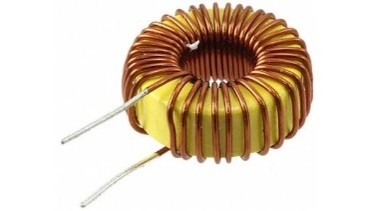
\includegraphics[width=0.8\textwidth]{Figures/Picture16.jpg}
        \caption{Toroidal Inductor Core}
    \end{minipage}\hfill
    \begin{minipage}{0.48\textwidth}
        \centering
        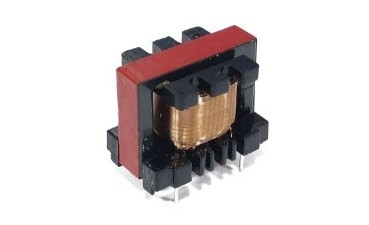
\includegraphics[width=0.7\textwidth]{Figures/Picture15.jpg}
        \caption{Wound Ferrite Inductor}
    \end{minipage}
\end{figure}

\begin{itemize}
    \item \textbf{Type:} Wound power inductors (core type selected according to current and switching frequency requirements).
    \item \textbf{Inductance Parameters:} Multiple values used, depending on the specific converter stage and its switching frequency.
    \item \textbf{Current Ratings:} Selected based on the maximum current expected to flow through each inductor without saturating the magnetic core boundaries.
\end{itemize}

\subsubsection{Application in the Project}
The power inductors form the main energy-storage element in the boost converter, buck converter, and two-quadrant chopper, storing energy from the source during the switch's ON state and releasing it to the load during the OFF state—this charge/discharge cycle is what enables the voltage step-up/step-down action of each converter. Selecting the appropriate inductance and current rating at each stage was necessary to ensure efficient energy transfer while keeping current ripple within acceptable limits.
\newpage
% -------------------------------------------------------------------------
\subsection{Capacitors}

\subsubsection{Description and Key Specifications}
Capacitors are passive components used to store electrical energy and smooth voltage variations. In this project, capacitors of different capacitance values and voltage ratings were used across the circuit—from small-value capacitors for decoupling and filtering at IC supply pins, to higher-value capacitors used for input/output filtering in the boost converter, buck converter, and two-quadrant chopper.

\begin{figure}[H]
    \centering
    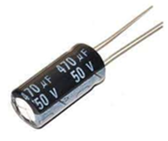
\includegraphics[width=0.4\textwidth]{Figures/Picture17.png}
    \caption{Through-Hole Radial Electrolytic Filter Capacitor Board Component.}
    \label{fig:capacitor}
\end{figure}

\begin{itemize}
    \item \textbf{Type:} Electrolytic and ceramic capacitors (through-hole style configurations).
    \item \textbf{Capacitance Range:} Multiple values used, ranging from sub-microfarad ceramic capacitors for noise decoupling up to higher-value electrolytic capacitors for converter filtering.
    \item \textbf{Voltage Safe Limits:} Selected according to the maximum voltage present at each point in the circuit, with an appropriate safety margin index.
\end{itemize}

\subsubsection{Application in the Project}
\begin{itemize}
    \item \textbf{Output Filtering:} Capacitors are placed at the output of each converter stage to smooth the switched voltage waveform, reducing ripple and providing a stable DC output to the next stage (battery, EV charging output, etc.).
    \item \textbf{Input Filtering:} Capacitors are also used at the input of converter stages to filter switching noise from feeding back into the PV array or battery source.
    \item \textbf{Decoupling:} Small-value capacitors are placed close to the supply pins of ICs, such as the IR2111 gate driver and the LM7812 regulator, to filter high-frequency noise and stabilize the supply voltage during fast switching transients.
\end{itemize}

\chapter{Control Methods}

% =========================================================================
% SECTION: CONTROL SYSTEM DESIGN FOR DC-DC CONVERTERS
% =========================================================================
\section{Control System Design for DC-DC Converters}

In an Electric Vehicle charging station integrated with Photovoltaic arrays, DC-DC converters must constantly adjust to shifting power demands. Because internal parts possess inherent electrical resistance, an increase in current causes the output voltage to naturally sag, potentially destabilizing the system. To solve this, a closed-loop feedback mechanism monitors these fluctuations and automatically widens the pulse-width modulation signals. This corrective action ensures the device maintains a consistent target voltage or current despite the dynamic and unpredictable nature of the connected load.

\subsection{Analytical Design vs. Trial-and-Error}
Utilizing mathematical modelling paired with deterministic frequency-response design offers an absolute engineering advantage over empirical ``trial-and-error'' tuning methods:

\begin{itemize}
    \item \textbf{Parametric Flexibility \& Scalability:} The control loop is completely parameterized. If any physical component changes (e.g., $R$, $L$, or $C$), you simply update the parameter value.
    \item \textbf{Rapid Re-Execution (Automated Scripting):} The entire script executes instantly to recalculate precise analog gains ($K_p$, $\omega_c$) and digital coefficients ($b_0$, $b_1$, $a_1$). This minimizes development cycle times.
\end{itemize}

\subsection{Voltage/Current Loop Control Design}
The closed-loop voltage control loop is designed systematically using the frequency response (loop-shaping) method. The entire procedure transitions from continuous-time analytical tuning to discrete difference equations ready for microcontroller firmware.

\newpage

\subsubsection{Hardware \& System Parameter Configurations}
The system configuration and open-loop transfer function variable initialization calculations are executed via the script setup below:

\begin{lstlisting}
%% circuit parameters
R = 10;          % Load resistance in ohms
rL = 1.9;        % Inductor resistance in ohms
rC = 0.2;        % Capacitor equivalent series resistance in ohms
Vo = 3.8;        % Output voltage in volts
Vin = 12.3;      % Input voltage in volts
rDS = 0.025;     % On-resistance of the switch in ohms
Vfwd = 0.8;      % Forward voltage drop of the diode in volts

%% Calculate the load current
Io = Vo / R;     % Output current in amps

%% Calculate the inductor current
iL = Io;         % Inductor current in amps

%% Calculate the duty cycle
Du = (Vfwd + iL * rL + Vo) / (Vin - iL * rDS + Vfwd);

%% Define the ripple specs
delta_iL = 0.6 * iL;     % Inductor current ripple in amps
delta_Vo = 0.02 * Vo;    % Output voltage ripple in volts

%% the switching frequency
fsw = 10e3;

%% the stress on components
Vd_stress = -Vin + iL * rDS;  % Diode stress voltage
Vsw_stress = Vin + Vfwd;      % Switch stress voltage
Id_stress = Io;               % Diode stress current
Isw_stress = Io;              % Switch stress current

%% inductance and capacitance values in design
L = 2e-3;
C = 220e-6;

%% Define the transfer function variable and plant GVdO
s = tf('s');
GVdO = (R * (C * rC * s + 1) * (Vfwd + Vin - iL * rDS)) / ...
       ((R + rL + Du * rDS + L * s + C * L * R * s^2 + ...
       C * L * rC * s^2 + C * R * rC * s + C * R * rL * s + ...
       C * rC * rL * s + C * Du * R * rDS * s + C * Du * rC * rDS * s));
\end{lstlisting}

\subsubsection{Frequency Response Specs: Phase Margin \& Crossover Frequency}

We begin by designing via the frequency response of the system, setting two main constraints: our desired phase margin and the target crossover frequency.

\begin{lstlisting}
%% Frequency Response Specs: Phase Margin & Crossover Frequency
CROSS_FREQ = 200;   % Crossover frequency in rad/s
des_PM = 90;        % Desired phase margin
fc_v = (CROSS_FREQ) / (2 * pi); % Crossover frequency
wc_v = CROSS_FREQ;

% Calculate the target phase margin in radians
targ_PM_v = deg2rad(des_PM);
\end{lstlisting}

\subsubsection{Evaluate Plant Phase at Crossover Frequency}
We want to compute the phase of the plant. We utilize the system's analytical plant transfer function ($G_{V_oD}$) to do this.

\begin{lstlisting}
%% Evaluate Plant Phase at Crossover Frequency
% Define the transfer function variable and plant GVdO
s = tf('s');
GVdO = (R * (C * rC * s + 1) * (Vfwd + Vin - iL * rDS)) / ...
       ((R + rL + Du * rDS + L * s + C * L * R * s^2 + ...
       C * L * rC * s^2 + C * R * rC * s + C * R * rL * s + ...
       C * rC * rL * s + C * Du * R * rDS * s + C * Du * rC * rDS * s));

% Evaluate the transfer function at the crossover frequency
gpc_v = evalfr(GVdO, wc_v * 1i);

% Calculate the gain and phase at the crossover frequency
gain_v = abs(gpc_v);
phase_v = angle(gpc_v);
\end{lstlisting}

\subsubsection{Determine Phase Compensation}
By subtracting the plant's phase from your target margin, you determine the required phase compensation ($pc\_v$). Since the resulting value is highly negative ($\approx -83.96^\circ$), it dictates a lag compensator profile.

\begin{lstlisting}
%% Determine Phase Compensation
% Calculate the phase compensation
pc_v = targ_PM_v - phase_v - pi;
\end{lstlisting}

\subsubsection{Calculate Integral and Proportional Components}
We calculate the integral component, then via trigonometric substitution, we calculate the proportional component while taking the overall plant gain into account. This solves for our two unknowns in our analog PI controller equation:

\begin{equation}
    G_c(s) = K_p \left( \frac{\omega_i}{s} + 1 \right)
\end{equation}

\begin{lstlisting}
%% Calculate Integral and Proportional Components
% Calculate the integral component
fi_v = -fc_v * tan(1 * pc_v);

% Calculate the proportional gain
Kp_v = (1 / gain_v) / sqrt((fi_v / fc_v)^2 + 1);

% Integral component in rad/s
wi_v = fi_v * 2 * pi;

% Define the compensator transfer function Gc_v
Gc_v = Kp_v * ((wi_v / s) + 1);
\end{lstlisting}

\subsubsection{Discretization via Bilinear Z-Transform}
Since this is an analog transfer function in the continuous $s$-domain, we need to transform it to the digital $z$-domain to run on a finite-time microcontroller. We apply the Bilinear Z-Transform:

\begin{equation}
    s = \frac{2}{T_s} \frac{z - 1}{z + 1}
\end{equation}

with a sampling frequency of 10 kHz ($T_s = \frac{1}{10000} = 100\ \mu\text{s}$). This maps our continuous poles and zeros into the discrete domain, yielding the digital transfer function coefficients ($b_0$, $b_1$, $a_1$).

\begin{lstlisting}
%% Discretization via Bilinear Z-Transform
% Discretize the compensator and open-loop transfer functions
Gc_v_d = c2d(Gc_v, 100);
\end{lstlisting}

\subsubsection{Stability Verification}
We view the closed-loop step response of our newly discretized system to make absolutely sure it remains stable, tracking the transient characteristics correctly before physical hardware deployment.

\begin{lstlisting}
%% Stability Verification
% step response of the closed-loop system
step(feedback(T_v_d, 1), 0.1);
\end{lstlisting}

\begin{figure}[H]
    \centering
    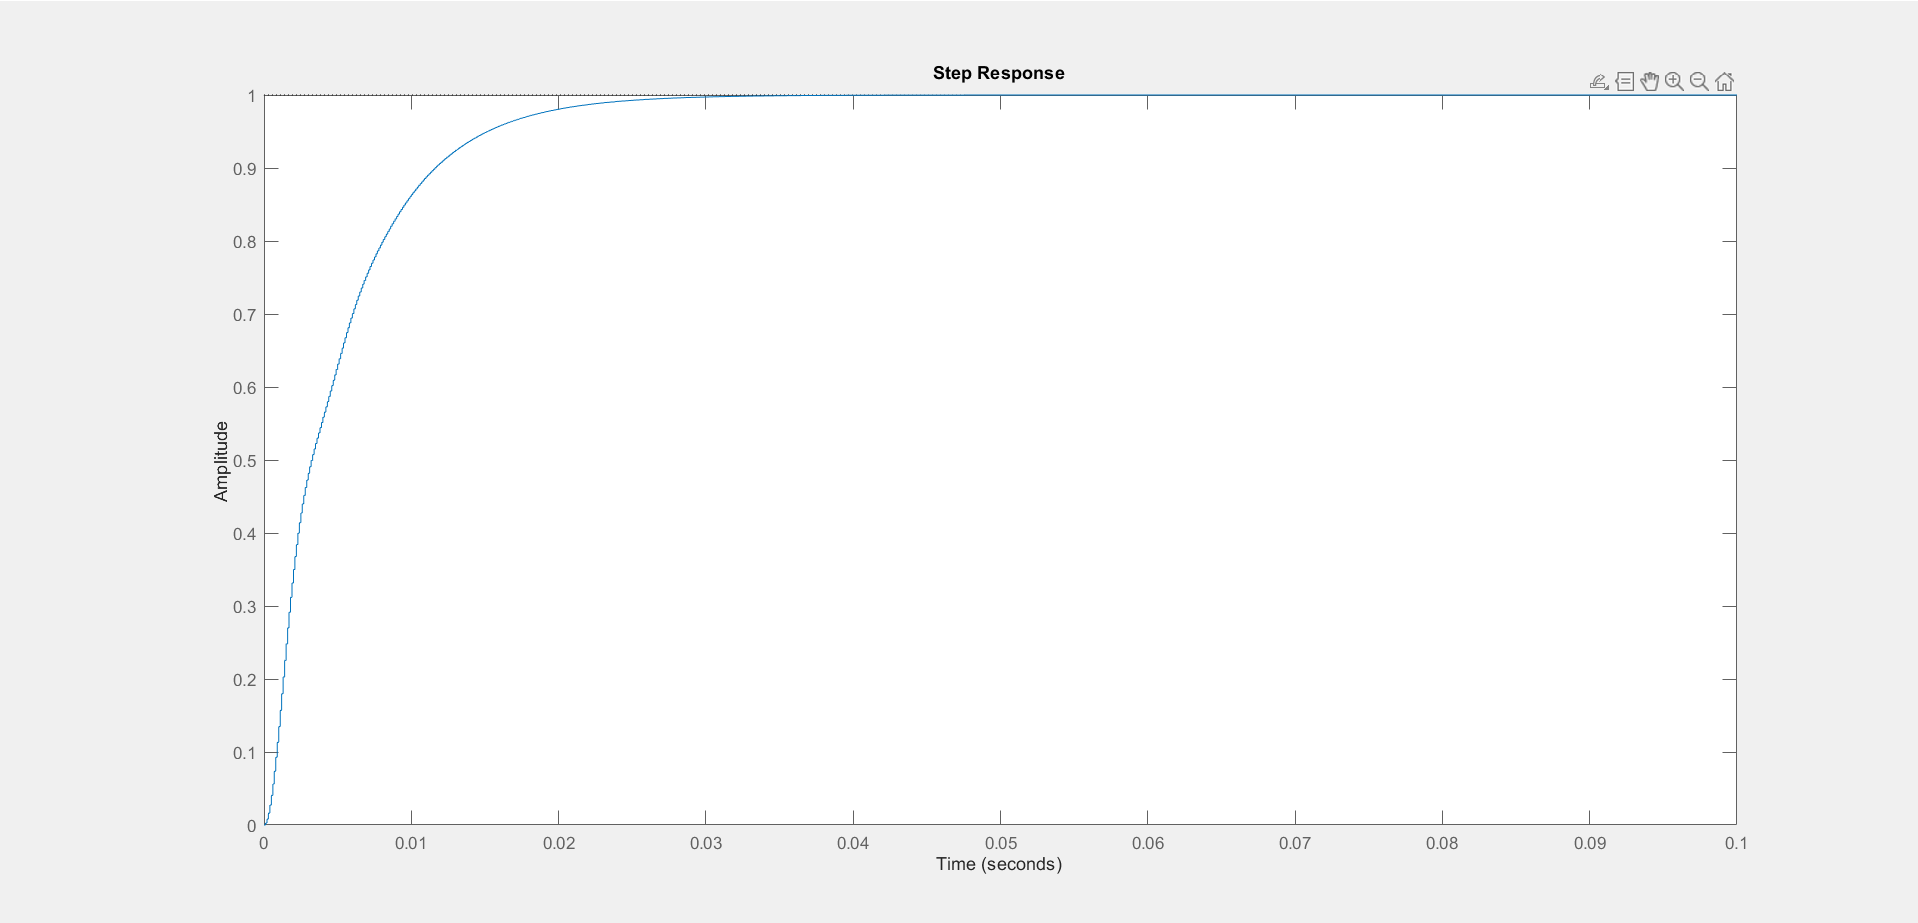
\includegraphics[width=0.9\textwidth]{Figures/step_response.png}
    \caption{Closed-loop system digital step response tracking.}
    \label{fig:control_step_response}
\end{figure}

\subsubsection{Frequency Response \& Stability Analysis (Bode Plot)}
We plot the Bode response of our system to verify the tracking performance, gain margin, and phase margin criteria under both continuous and discretized loop conditions.

\begin{lstlisting}
%% Frequency Response & Stability Analysis (Bode Plot)
% Bode plots for the transfer functions
margin(GVdO);    % Uncompensated Plant
margin(T_v);     % Continuous-time Open-Loop System
margin(T_v_d);   % Discretized Open-Loop System
\end{lstlisting}

\begin{figure}[H]
    \centering
    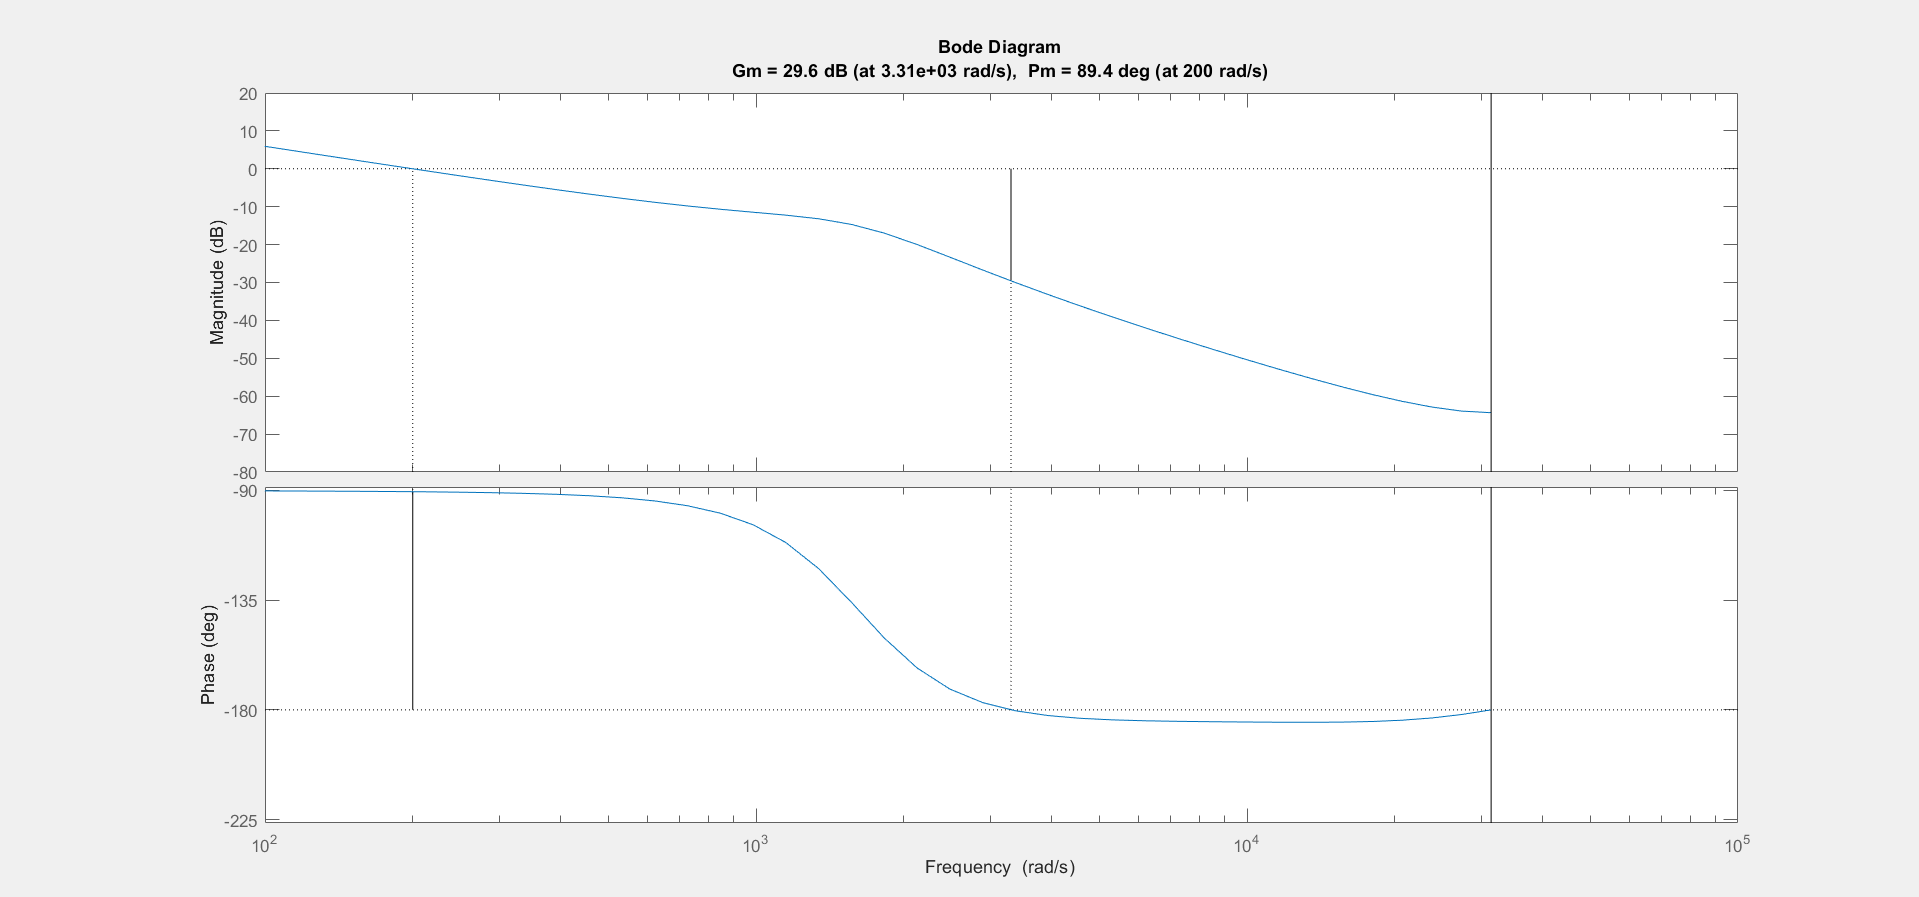
\includegraphics[width=0.9\textwidth]{Figures/bode_plot.png}
    \caption{System Bode diagram highlighting phase and gain margins.}
    \label{fig:control_bode_plot}
\end{figure}

\chapter{Simulation Results}
% =========================================================================
% SECTION 5.1: interleaved boost converter simulation
% =========================================================================

\section{Central and String Interleaved Boost with Load (High Ratings)}

\subsection{Introduction}
In the field of modern electrical engineering, the transition from theoretical mathematical equations to tangible physical hardware represents one of the most critical and challenging phases of a graduation project. Designing advanced power electronics, control algorithms, and renewable energy systems involves managing highly non-linear dynamics, transient phenomena, and delicate hardware components. In a practical laboratory setting, executing direct "trial-and-error" testing on real hardware is not only financially prohibitive but also poses significant safety risks, as minor controller errors can lead to catastrophic component failures. Therefore, engineering design requires a reliable and intermediate validation phase to guarantee system safety and performance before hardware implementation.

To bridge this gap between theory and hardware,simulation has become an indispensable tool in engineering research and education. Simulation software allows us to build precise mathematical twins of physical components—such as photovoltaic arrays, switching converters, and closed-loop controllers—and observe their behavioral dynamics under safely controlled conditions. It provides the unique capability to test worst-case operational scenarios, analyze transient responses, and fine-tune controller coefficients without the risk of damaging expensive laboratory equipment.

For this project, MATLAB and Simulink were selected as the primary simulation ecosystem. MATLAB’s powerful numerical computing engine, combined with Simulink’s specialized Simscape Electrical libraries, allows for the seamless integration of physical power hardware with complex control logic. From executing high-speed Pulse Width Modulation (PWM) to designing multi-state Global Maximum Power Point Tracking (GMPPT) algorithms, MATLAB enables us to thoroughly debug code, verify system stability, and optimize electrical performance. Ultimately, the simulation framework developed in this work serves as the foundational blueprint, providing the rigorous analytical validation necessary to transition our designs into a successful, real-world engineering reality.
\newpage

\subsection{PV array distribution}

\subsubsection{Power calculation}
If per day energy needed = 42.5 KW.h, so the power needed from PV array = 8500W (regarding that the sun remains at its peak intensity for five hours).

This PV specification meets the requirements:
\begin{figure}[H]
    \centering
    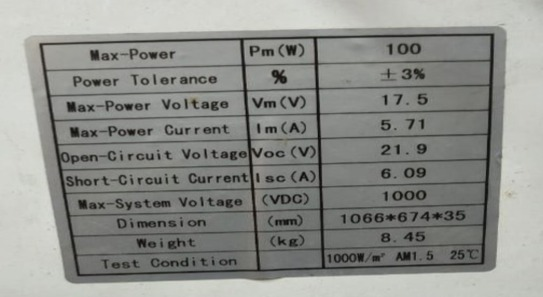
\includegraphics[width=0.75\textwidth]{Figures/PV1.jpg}
    \caption{PV specification.}
    \label{fig:PV specification}
\end{figure}
\begin{equation}
    P_{\text{module}} = V_m \times I_m = 40.9\,\text{V} \times 17.36\,\text{A} = 710\,\text{W}
\end{equation}
\begin{equation}
    \text{Number of modules} = \frac{8500\,\text{W}}{710\,\text{W}} \approx 12\text{ Panels}
\end{equation}
\subsubsection{PV configuration}
The photovoltaic system simulation is initiated by defining the standard environmental parameters. As shown in Figure 5.2, the PV array block receives two primary environmental inputs: a constant solar irradiance (Ir) of 1000 W/m2 and a cell temperature (T) of 25°C, representing Standard Test Conditions (STC).
Connected across the output terminals of the PV block is an anti-parallel diode acting as a bypass protection layer against partial shading conditions and potential hot-spot development. To stabilize the DC bus voltage and mitigate high-frequency transient ripple resulting from downstream switching operations, an RC network consisting of a series resistor and a parallel capacitor is integrated at the PV output interface.
\begin{figure}[H]
    \centering
    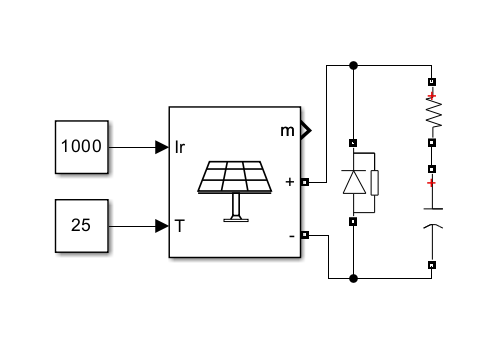
\includegraphics[width=0.75\textwidth]{Figures/PV configuration.png}
    \caption{PV configuration.}
    \label{fig:PV configuration}
\end{figure}
\begin{figure}[H]
    \centering
    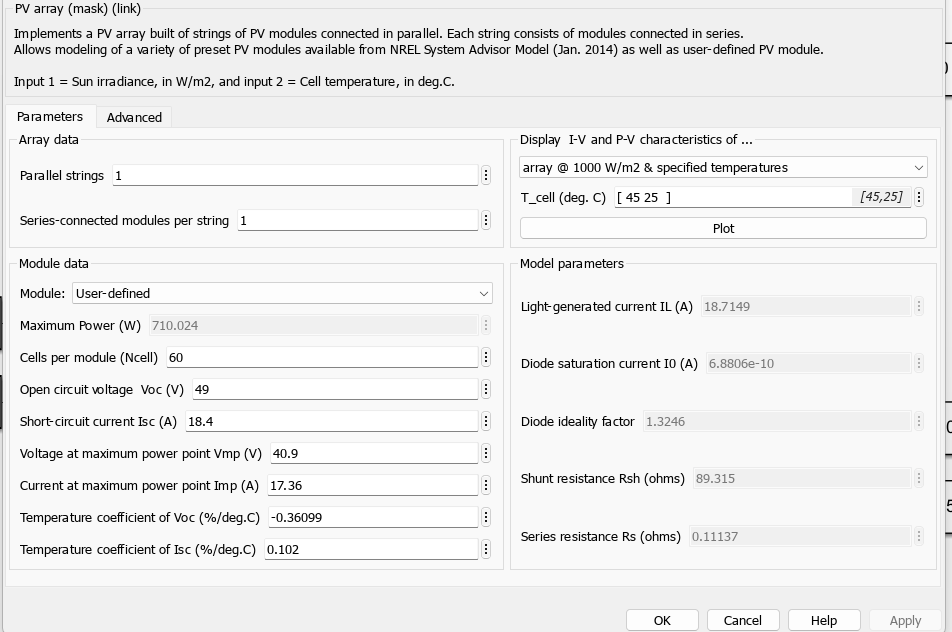
\includegraphics[width=1\textwidth]{Figures/spec.png}
    \caption{PV block specifications.}
    \label{fig:PV block specifications}
\end{figure}

\newpage
\subsubsection{Array configuration}
The general rules for array sizing are:
\begin{itemize}
  \item $N_s$ (number of modules in series) increases array voltage:
        $V_{\text{array}} = N_s \times V_{\text{module}}$
  \item $N_p$ (number of parallel strings) increases array current:
        $I_{\text{array}} = N_p \times I_{\text{module}}$
\end{itemize}
 \begin{table}[htbp]
    \centering
    \caption {Different ways to distribute these twelve modules:}
    \label{tab:pv_configurations}
    \small
    \begin{tabular}{|c|c|c|c|}
        \hline
        \textbf{Configuration ($N_s \times N_p$)} & \textbf{Voltage ($V$)} & \textbf{Current ($I$)} & \textbf{Power ($W$)} \\ \hline
        1 * 12 & 490.8 & 17.36  & 8520 \\ \hline
        2 * 6  & 245.4 & 34.72  & 8520 \\ \hline
        3 * 4  & 163.6 & 52.08  & 8520 \\ \hline
        4 * 3  & 122.7 & 69.44  & 8520 \\ \hline
        6 * 2  & 81.8  & 104.16 & 8520 \\ \hline
        12 * 1 & 40.9  & 208.32 & 8520 \\ \hline
    \end{tabular}
\end{table}
Configuration 1 or Configuration 2 are the best choices. They keep the voltage high enough to match the input DC-link requirements of standard inverters while keeping current low, which minimizes power losses across the transmission cables.
To show the difference between central and string configurations, configuration 2 will be used in simulation.
\subsection{Central Configuration with Load}
In this configuration, a number of series PV arrays are connected in a central manner, which means the positive terminal of each string are connected and the negative terminals are also connected.
In central configuration only one boost converter is used to step up the voltage for the whole system from 245.4V to 600V as the battery of EV is 400V so the dc link voltage must be more than 400V.
\begin{figure}[H]
    \centering
    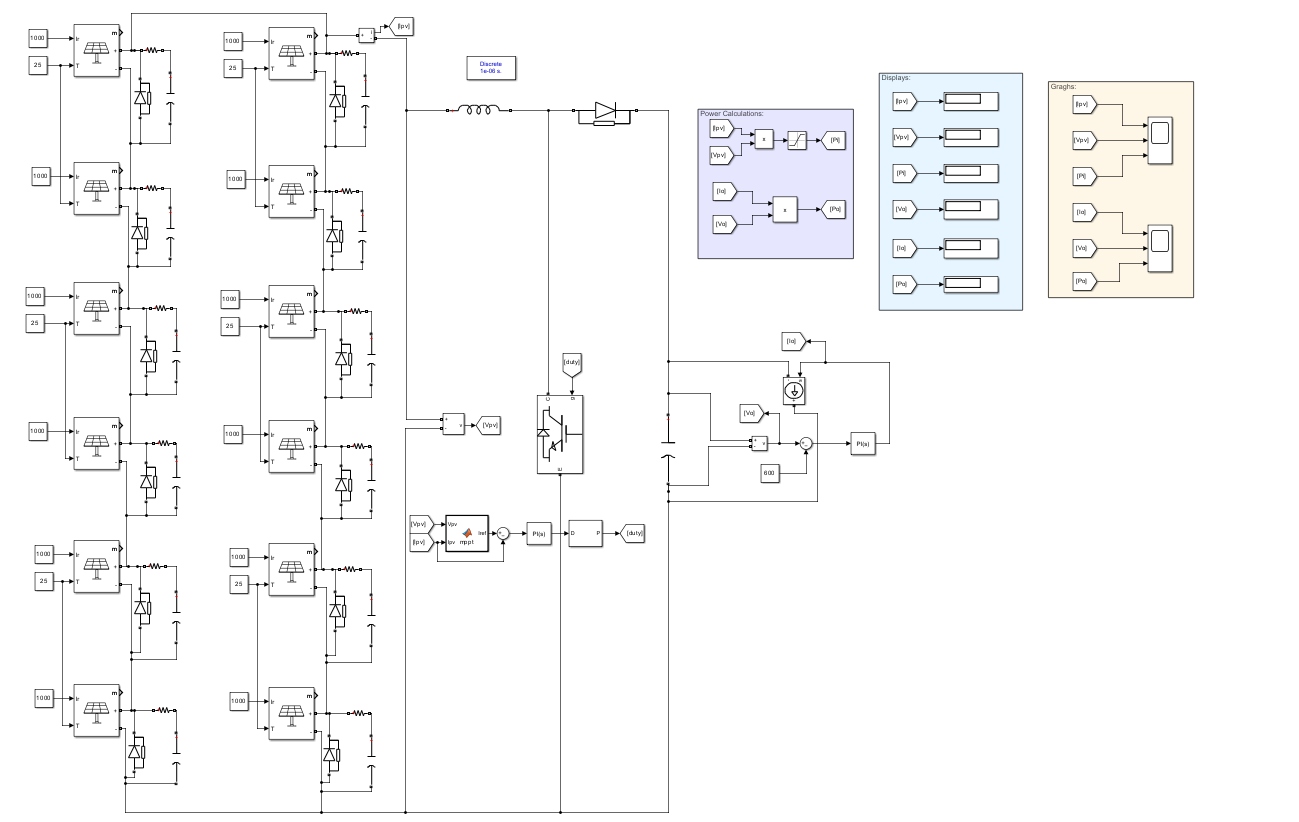
\includegraphics[width=1\textwidth]{Figures/central1.png}
    \caption{Central array configuration.}
    \label{fig:central array configuration.}
\end{figure}
\subsubsection{Boost Converter}
Boost converter is used to boost the input voltage from 245.4V (40.9*6) to 600V that will be used in the DC link to charge Electric Vehicles.
Calculations can be shown as follows:
\begin{align}
  D &= 1 - \frac{V_{\text{in}}}{V_{\text{out}}} = 1 - \frac{245.4}{600} = 0.591 \\[4pt]
  f_s &= \SI{10}{\kilo\hertz} \\[4pt]
  R &= \frac{V_{\text{out}}}{I_{\text{out}}} = \frac{600}{13.9} = \SI{43.165}{\ohm} \\[4pt]
  L_{\min} &= \frac{R \cdot D \cdot (1-D)^2}{2\,f_s}
             = \frac{43.165 \times 0.591 \times (0.409)^2}{2 \times 10000}
             \approx \SI{0.213}{\milli\henry} \\[4pt]
  \Delta I_L &= \frac{V_{\text{in}} \cdot D}{L \cdot f_s}
              = \frac{245.4 \times 0.591}{0.015 \times 10000}
              \approx \SI{0.967}{\ampere}
\end{align}

A practical inductance of $L = \SI{15}{\milli\henry}$ is chosen, well above $L_{\min}$, to ensure
continuous conduction mode (CCM) with a comfortable margin.

\medskip
\newpage
\noindent\textbf{Output Capacitor (DC-link):} A bulk capacitor of $C = \SI{50e-3}{\farad}$
is selected because:
\begin{itemize}
  \item It filters high-frequency switching noise to provide a stable, constant \textbf{600\,V} DC output.
  \item It stores energy to support the system during sudden changes in solar power or load demand.
  \item It minimises voltage ripple, ensuring the power delivered to the next stage is clean and steady.
\end{itemize}

\subsubsection{MPPT Implementation}
\begin{figure}[H]
    \centering
    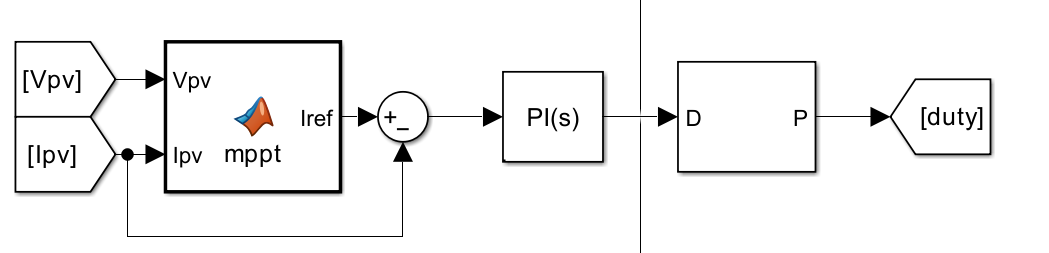
\includegraphics[width=1\textwidth]{Figures/mppt.png}
    \caption{MPPT Implementation.}
    \label{fig:MPPT Implementation.}
\end{figure}
\paragraph{Stage 1 — Current Reference Generation}
\begin{itemize}
  \item The MPPT function takes two inputs $V_{pv}$ (panel voltage) and $I_{pv}$ (panel
        current) and outputs $I_{\text{ref}}$, the reference current that controls how
        much power is drawn from the panel.
  \item The actual measured current is subtracted from $I_{\text{ref}}$ to produce an
        error signal. A continuous-time PI controller ($K_p = 0.05$, $K_i = 10$)
        processes this error to eliminate steady-state offset and smooth the response.
        Because the PI output is in amperes, and the DC-DC converter operates only on a
        duty cycle (a dimensionless number between 0 and 1), a further conversion stage
        is required.
\end{itemize}

\paragraph{Stage 2 — Duty Cycle Generation}
\begin{itemize}
  \item \textbf{D (divider):} Normalises the PI output by dividing by $V_{pv}$. From
        the boost-converter inductor ripple equation,
        $\Delta I_L = V_{\text{in}}\,D\,/\,(L\,f_s)$, the same duty cycle produces
        different currents at different input voltages. Dividing by $V_{pv}$ removes
        this dependency so the control loop behaves identically across the full
        operating voltage range.
  \item \textbf{P (gain block):} Scales the small dimensionless result into the $[0,1]$
        range expected by the PWM generator.
  \item The final output is the duty cycle signal sent to the boost converter switch.
\end{itemize}
\newpage
\paragraph{How the code works}
\begin{lstlisting}[language=Matlab, caption={MATLAB code implementing the FSM-based global MPPT control loop.}]
function Iref = mppt(Vpv, Ipv)
    persistent V_target Pmax Vbest mode timer;
    
    Ts = 1e-6;
    
    % Voltage sweep parameters - sweep Vpv from high to low
    V_oc_est = 280;           % Estimated open circuit voltage
    V_scan_min = 240;         % Minimum scan voltage
    V_ramp_rate = 150;        % V/s sweep rate
    
    if isempty(V_target)
        V_target = V_oc_est;
        Pmax = 0;
        Vbest = 240;          % Start with nominal MPP voltage
        mode = 0;
        timer = 0;
    end
    
    Ppv = Vpv * Ipv;
    
    switch mode
        case 0  % RESET - go to high voltage (low current)
            V_target = V_oc_est;
            Pmax = 0;
            if Vpv > 270       % Near Voc
                mode = 1;
            end
            
        case 1  % SCAN - sweep voltage DOWN to find global Pmax
            % Record power at each voltage
            if Ppv > Pmax
                Pmax = Ppv;
                Vbest = V_target;
            end
            
            V_target = V_target - (V_ramp_rate * Ts);
            
            if V_target <= V_scan_min
                mode = 2;
            end
            
        case 2  % RETURN to Vbest
            if V_target < Vbest
                V_target = V_target + (300 * Ts);
            else
                V_target = Vbest;
                mode = 3;
                timer = 0;
            end
            
        case 3  % HOLD
            timer = timer + Ts;
            if timer >= 5
                mode = 0;
            end
    end
    
    % INNER LOOP: Current controller to regulate Vpv to V_target
    % Simple P-control: if Vpv > V_target, increase current (load more)
    %                  if Vpv < V_target, decrease current (load less)
    persistent err_int;
    if isempty(err_int), err_int = 0; end
    
    err = Vpv - V_target;           % Positive = need more load
    err_int = err_int + err * Ts;
    err_int = max(min(err_int, 50), -50);  % Anti-windup
    
    Kp = 1;   % Proportional gain
    Ki = 200;   % Integral gain
    
    % Base current + correction
    I_calc = 20 + Kp * err + Ki * err_int;
    
    % Limit output
    Iref = max(min(I_calc, 35), 0);
end
\end{lstlisting}

\medskip
\noindent\textbf{Code Operation Breakdown:}
\begin{itemize}
    \item \textbf{Lines 2--10:} Initialize persistent tracking metrics and operational variables. These memory boundaries ensure tracking parameters are preserved across discrete high-speed execution frames ($T_s = 1\ \mu\text{s}$). A voltage ramp rate of $V_{\text{ramp\_rate}} = 150\text{ V/s}$ combined with a sample time of $T_s = 1\ \mu\text{s}$ means that the target voltage drops by exactly $150 \times 10^{-6} = 0.00015\text{ V}$ per execution step. This configuration results in an extremely fine-grained sweep profile that prevents the tracking algorithm from missing narrow global power peaks.
    
    \item \textbf{Lines 11--17:} Execute the baseline cold-start routine exactly once at simulation startup. This block sets the initial target voltage near the open-circuit threshold, resets the captured power registers to zero, and forces a direct transition into the tracking loop.
    \newpage
    \item \textbf{Lines 21--27:} Mode 0 (Reset Routine): The algorithm establishes a high boundary threshold target voltage ($V_{\text{target}} = 270\text{ V}$) where the converter circuit draws approximately zero current from the source terminals.Once the measured PV array voltage stabilizes and settles within proximity of this open-circuit reference point, the sequential sweep routine is automatically triggered.
    
    \item \textbf{Lines 29--40:} Mode 1 (Global Scan Phase): The algorithm dynamically forces the operational target voltage reference to decrease linearly across the predefined sweeping region. As the voltage is pulled down, the controller evaluates the instantaneous power extraction profile ($P_{\text{pv}} = V_{\text{pv}} \times I_{\text{pv}}$). If the instantaneous computed power exceeds the highest previously logged power value ($P_{\text{max}}$), the internal registers overwrite the historical maximum with the updated peak value ($P_{\text{max}} = P_{\text{pv}}$) and log the exact voltage coordinate as the optimal reference ($V_{\text{best}} = V_{\text{pv}}$).
    
    \item \textbf{Lines 42--49:} Mode 2 (Peak Return Phase): The linear global scanning sweep terminates automatically once the target tracking voltage descends to its lower operational bound ($240\text{ V}$). Upon reaching this threshold, the state machine shifts execution modes and systematically ramps the reference voltage back upward until it perfectly aligns with the captured optimal tracking coordinate ($V_{\text{best}}$).
    
    \item \textbf{Lines 51--56:} Mode 3 (Maximum Power Point Hold): The controller latches onto $V_{\text{best}}$ and holds this steady profile for a fixed duration of $5\text{ s}$ to maximize steady-state energy extraction without hunting oscillations. When the tracking timer expires, the block loops back to Mode 0 to re-evaluate the global P-V curve for updated atmospheric or partial shading alterations.
    
    \item \textbf{Lines 58--76:} Closed-Loop Reference Control Tracking: A continuous Proportional - Integral (PI) feedback loop ensures the actual physical panel voltage ($V_{\text{pv}}$) remains dynamically locked onto the tracking reference command ($V_{\text{target}}$) by actively adjusting the current reference output ($I_{\text{ref}}$):
    \begin{itemize}
        \item \textbf{Case A ($V_{\text{pv}} > V_{\text{target}}$):} The resulting error signal evaluates as positive. The loop increases the output current reference ($I_{\text{ref}}$) to draw more power from the PV array, which unloads the voltage down toward the target.
        \item \textbf{Case B ($V_{\text{pv}} < V_{\text{target}}$):} The error evaluates as negative. The controller decreases $I_{\text{ref}}$ to unload the array, allowing the internal cell capacitance to charge up toward the desired command.
    \end{itemize}
    To counter integrator windup and prevent mathematical saturation under transient changes, an anti-windup clamping threshold ($\pm 50$) is applied directly to the integration accumulator, while the reference output current command ($I_{\text{ref}}$) is strictly capped between $0\text{ A}$ and $35\text{ A}$ to protect downstream hardware components from overcurrent damage.
\end{itemize}
\newpage
\subsubsection{DC Link Voltage}
The control system ensures the output voltage remains constant at 600V by employing a feedback loop that compares the measured DC-link voltage with a 600V reference signal. The resulting error is processed by a PI Controller, which generates the necessary power or current commands to balance the energy flow. This regulation is vital to stabilize the DC bus against fluctuations in solar irradiance and load variations, ensuring the system operates at its designed 8520W peak power efficiently.

\subsubsection{Results of Simulation in Case of No Shading}
\noindent
\begin{minipage}[t]{0.5\textwidth}
\vspace{0pt}
\begin{itemize}
  \item As shown, current is almost $17.36 \times 2$, the input voltage is also aligned
        with design calculations and output power is 8419\,W, ideally should be 8520\,W,
        but there are switching losses and conduction losses (diodes have forward voltage,
        etc.).

  \item \textbf{DC-Link Stability:} The output voltage ($V_{DC}$) is maintained at
        exactly 600\,V. This proves that the DC-Link Voltage Control loop
        ($K_p = 3$, $K_i = 50$) and the Bulk Capacitor are effectively regulating the
        output despite the high-power flow.

  \item Ripples of inductor current $= 35.18 - 34.2 = 0.98$\,A.
\end{itemize}
\end{minipage}
\hfill
\begin{minipage}[t]{0.4\textwidth}
\vspace{0pt}
  \centering
  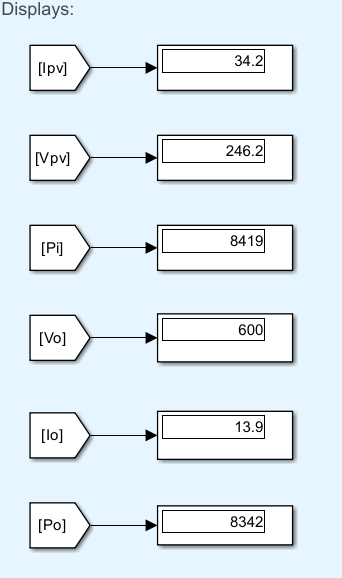
\includegraphics[width=\textwidth]{Figures/displaycentral1.png}
  \captionof{figure}{Displays of central configuration at no shading.}
  \label{fig:Displays of central configuration at no shading}
\end{minipage}
\paragraph{Graphs}
\begin{figure}[H]
    \centering
    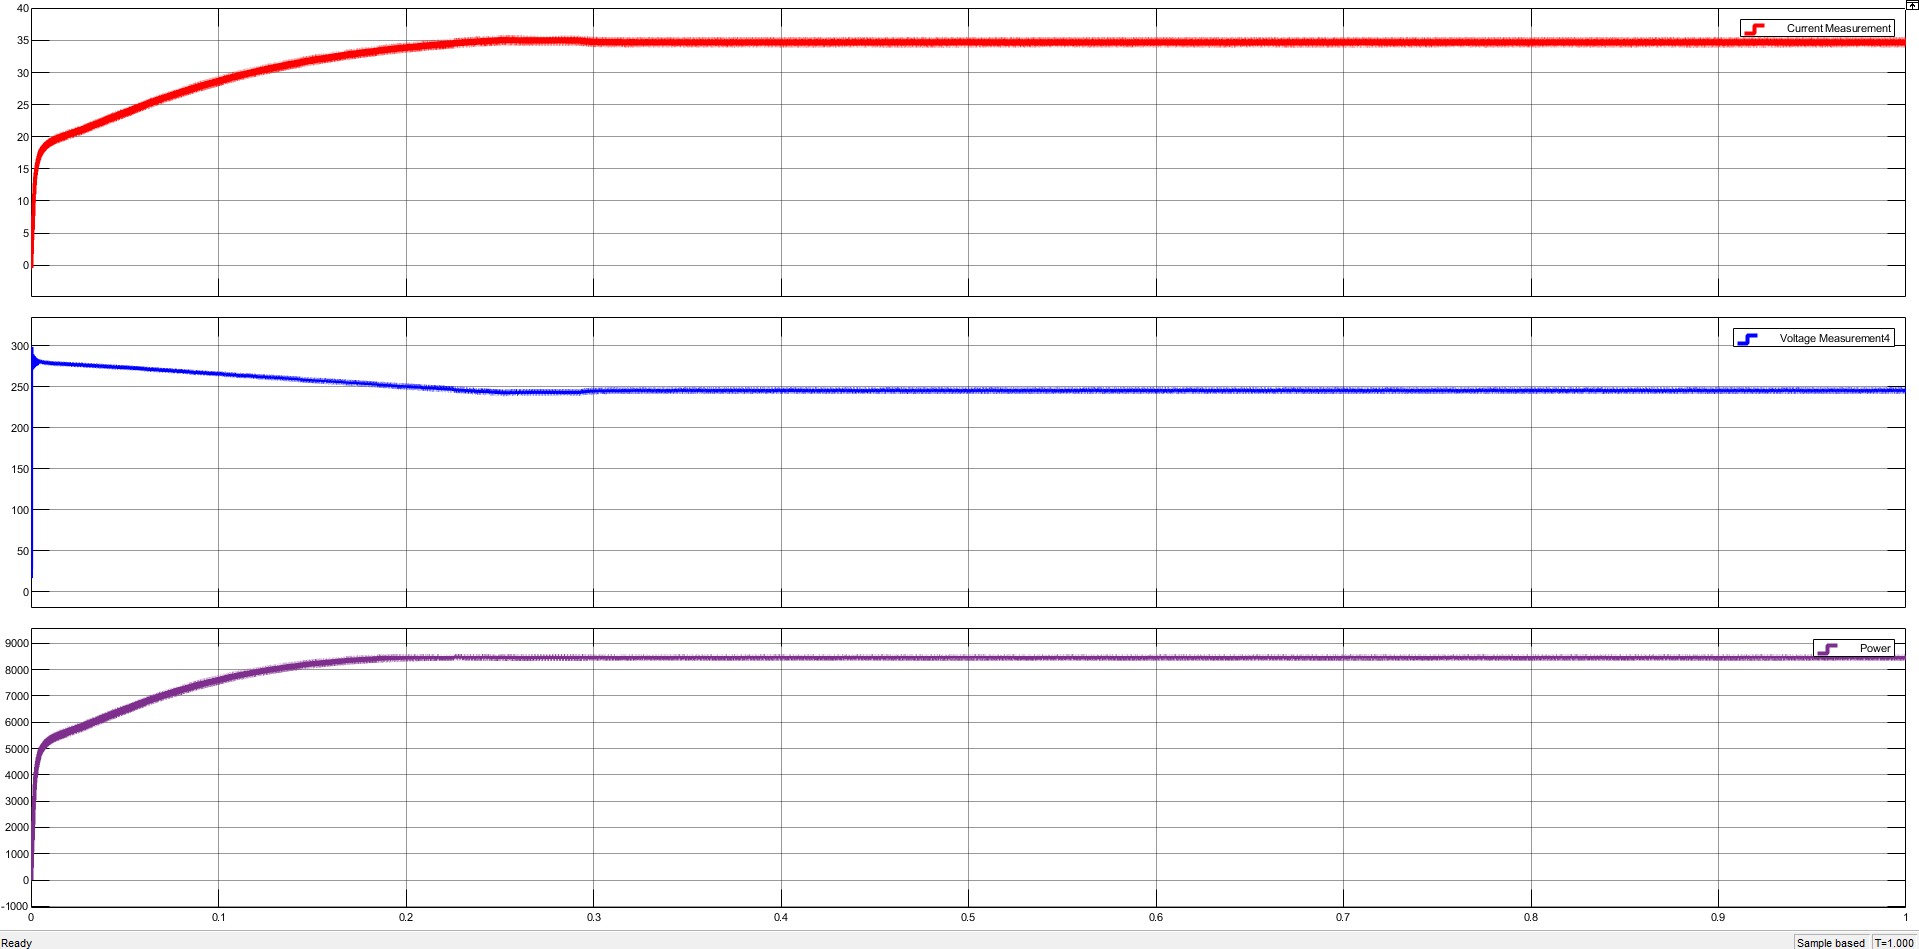
\includegraphics[width=1.1\textwidth]{Figures/5.1.7.png}
    \caption{Input current, voltage, power at no shading.}
    \label{fig:Input current, voltage, power at no shading}
\end{figure}
\begin{figure}[H]
    \centering
    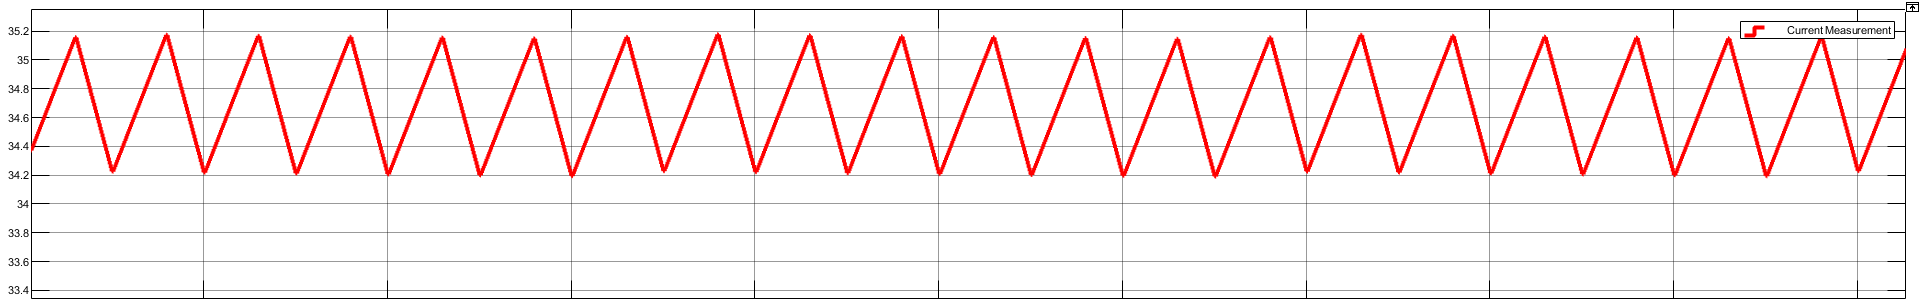
\includegraphics[width=1.1\textwidth]{Figures/5.1.8.png}
    \caption{Ripples of inductor current at no shading.}
    \label{fig:Ripples of inductor current at no shading}
\end{figure}
\begin{figure}[H]
    \centering
    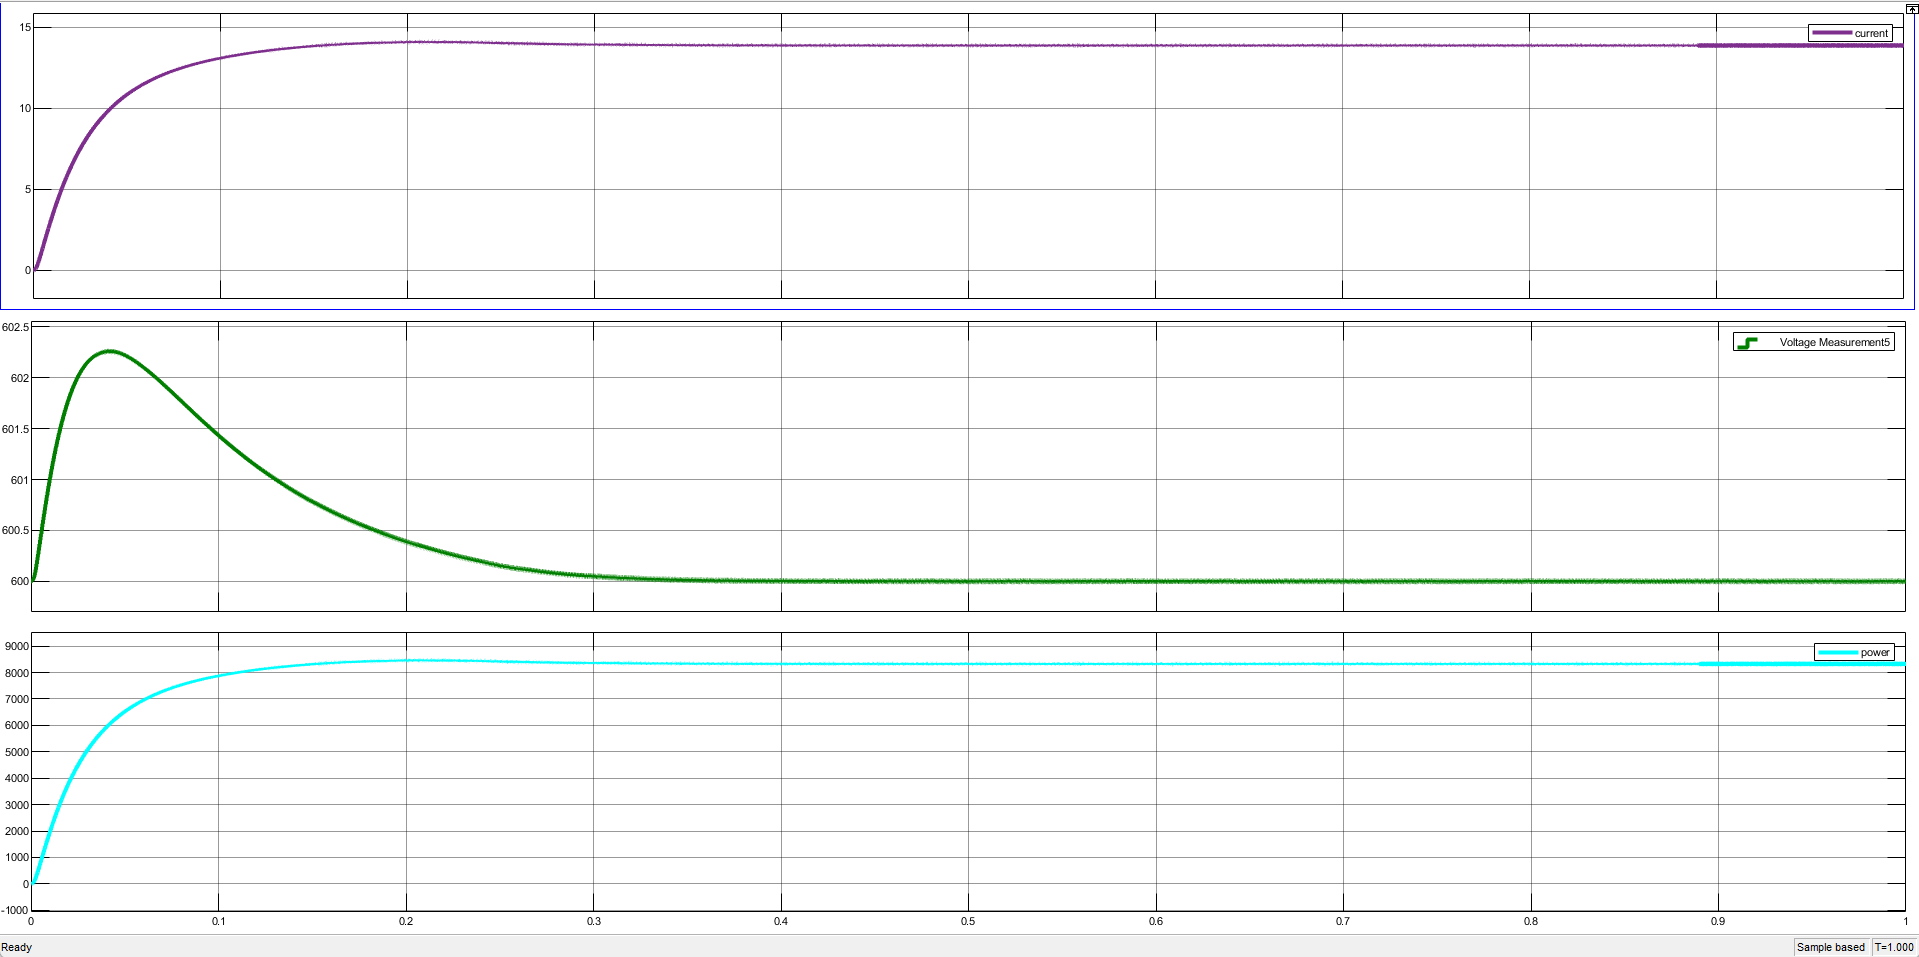
\includegraphics[width=1.1\textwidth]{Figures/5.1.9.png}
    \caption{Output current, voltage, power at no shading.}
    \label{fig:Output current, voltage, power at no shading}
\end{figure}

\subsubsection{Results of Simulation in Case of Shading (Ir = 800) at One Module}
\noindent
\begin{minipage}[t]{0.5\textwidth}
\vspace{0pt}
\begin{itemize}
  \item As shown, the output power decreases as the current decreases, but the Vpv is almost constant.
  \item Dc link voltage still maintained at 600\,V due to closed loop with PI.
  \item Ripples of inductor current $= 31.8 - 31 = 0.8$\,A.
\end{itemize}
\end{minipage}
\hfill
\begin{minipage}[t]{0.4\textwidth}
\vspace{0pt}
  \centering
  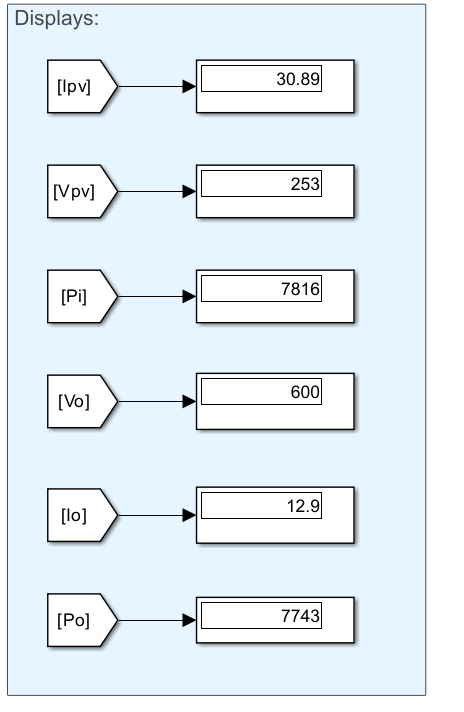
\includegraphics[width=\textwidth]{Figures/5.1.10.png}
  \captionof{figure}{Displays of central configuration at 800 shading.}
  \label{fig:Displays of central configuration at 800 shading}
\end{minipage}
\paragraph{Graphs}
\begin{figure}[H]
    \centering
    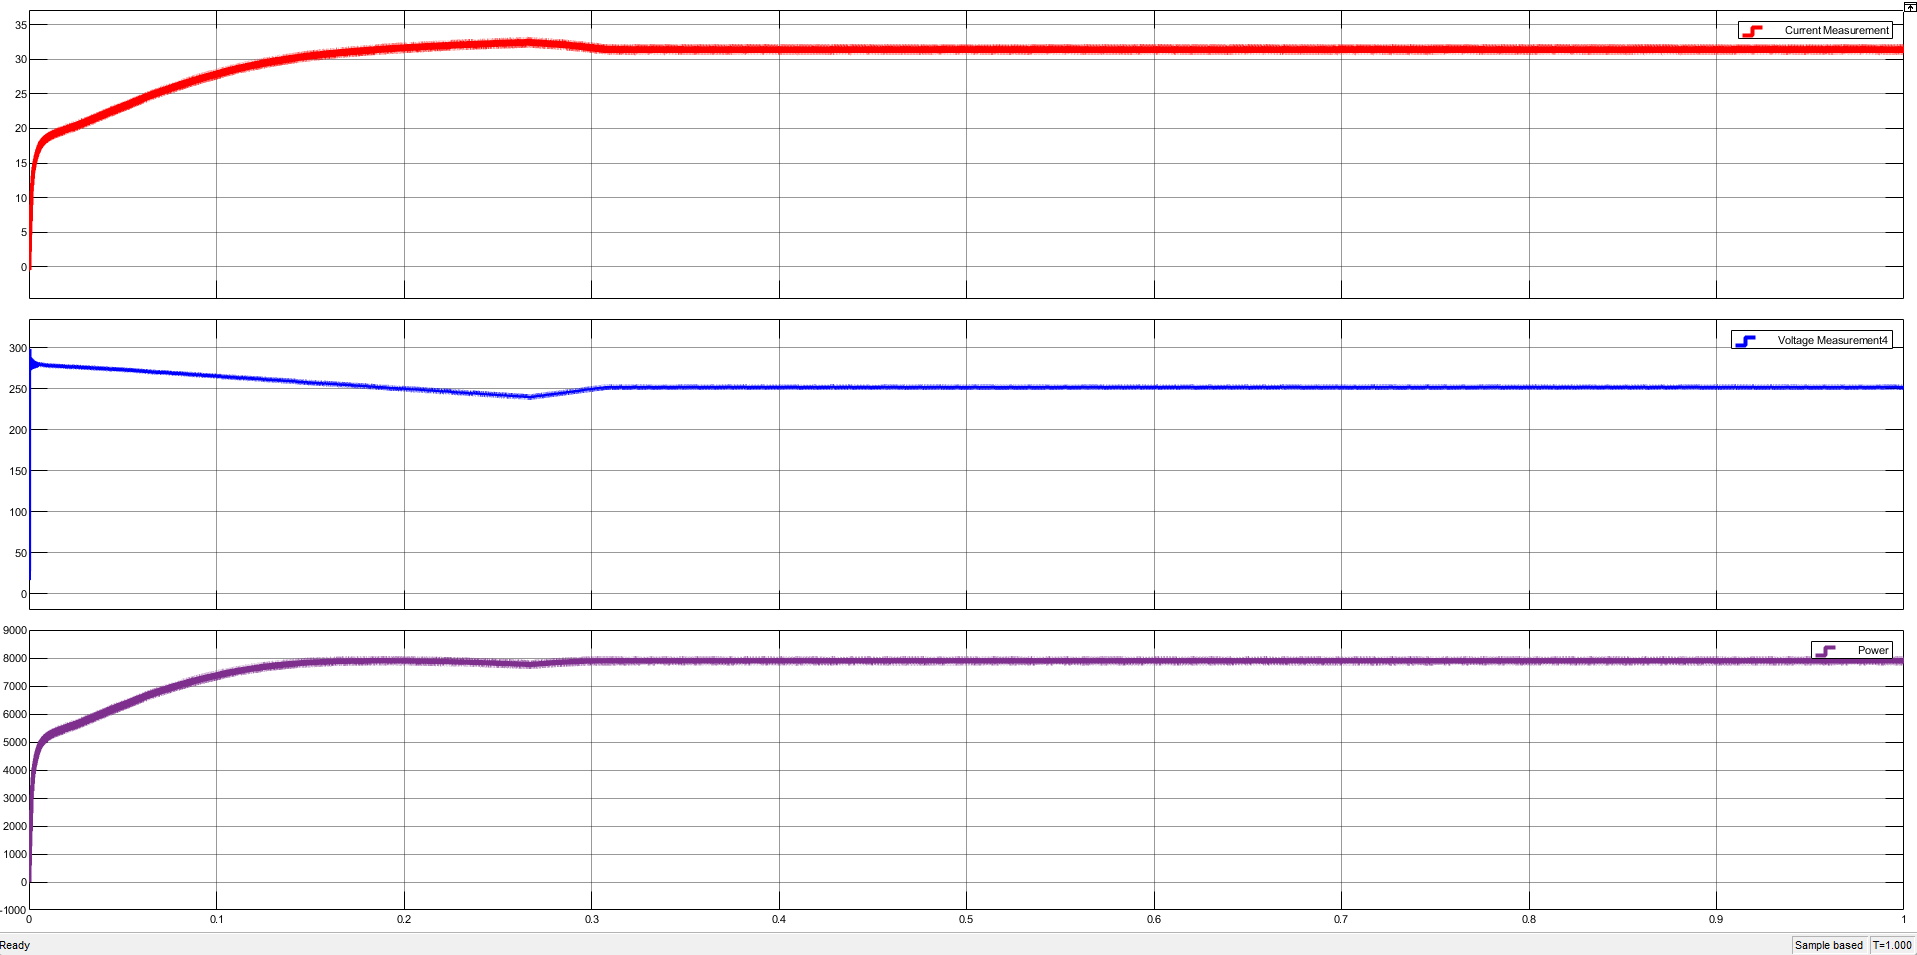
\includegraphics[width=1.1\textwidth]{Figures/5.1.11.png}
    \caption{Input current, voltage, power at 800 shading.}
    \label{fig:input current, voltage, power at 800 shading}
\end{figure}
\begin{figure}[H]
    \centering
    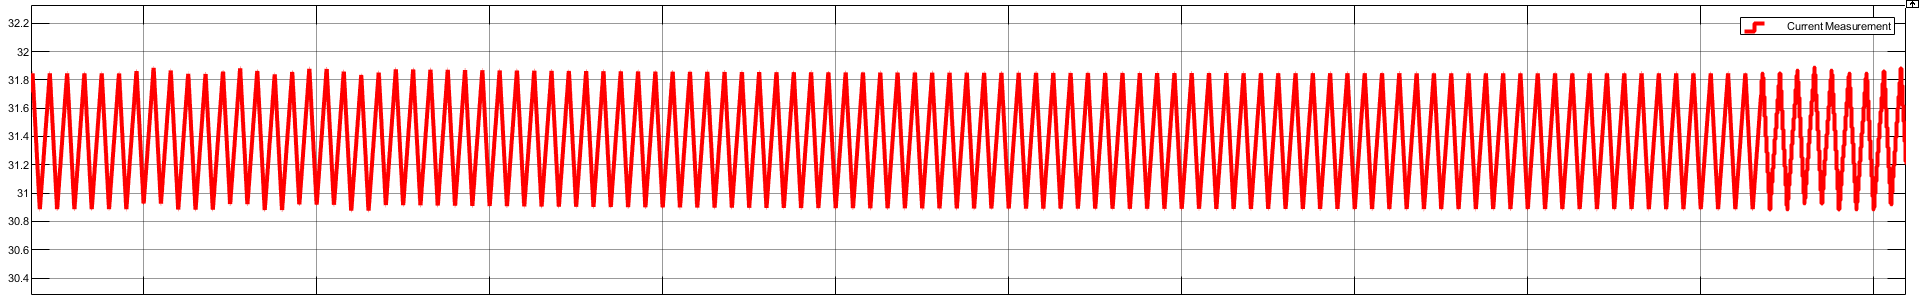
\includegraphics[width=1.1\textwidth]{Figures/5.1.12.png}
    \caption{Ripples of inductor current at 800 shading.}
    \label{fig:ripples of inductor current at 800 shading}
\end{figure}
\begin{figure}[H]
    \centering
    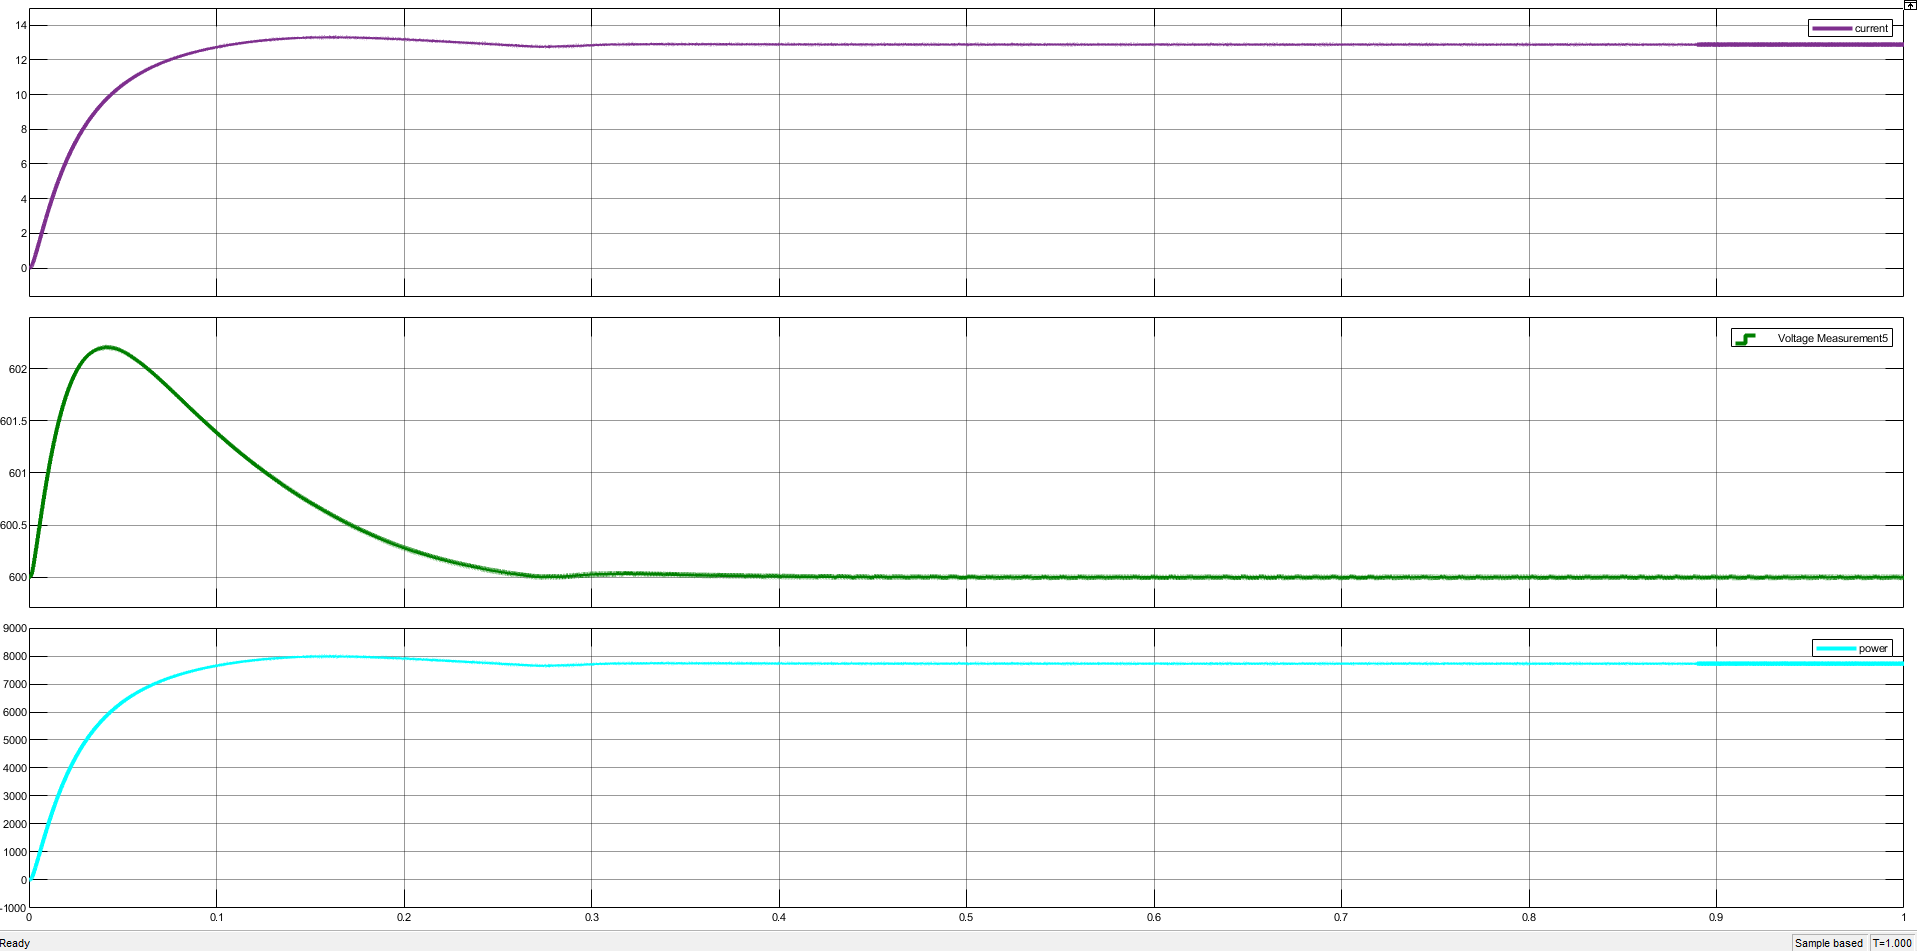
\includegraphics[width=1.1\textwidth]{Figures/5.1.13.png}
    \caption{Output current, voltage, power at 800 shading.}
    \label{fig:Output current, voltage, powerat 800 shading}
\end{figure}

\subsubsection{Results of Simulation in Case of Shading (Ir = 500) at One Module}
\noindent
\begin{minipage}[t]{0.5\textwidth}
\vspace{0pt}
\begin{itemize}
  \item As shown, the output power decreases much more as the current decreases more than the current in the pervious case as Ir decreases, but the Vpv is almost constant.
  \item Dc link voltage still maintained at 600V due to closed loop with PI.
  \item Ripples of inductor current $= 26.7 - 25.8 = 0.9$\,A.
\end{itemize}
\end{minipage}
\hfill
\begin{minipage}[t]{0.4\textwidth}
\vspace{0pt}
  \centering
  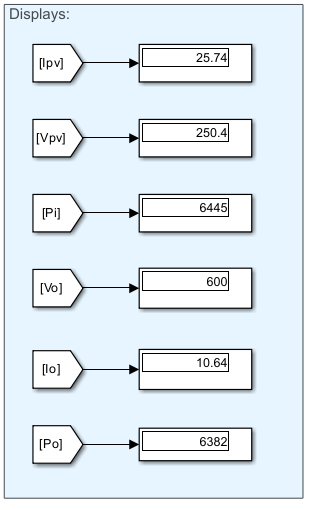
\includegraphics[width=\textwidth]{Figures/5.1.14.png}
  \captionof{figure}{Displays of central configuration at 500 shading.}
  \label{fig:Displays of central configuration at 500 shading}
\end{minipage}
\paragraph{Graphs}
\begin{figure}[H]

\centering
    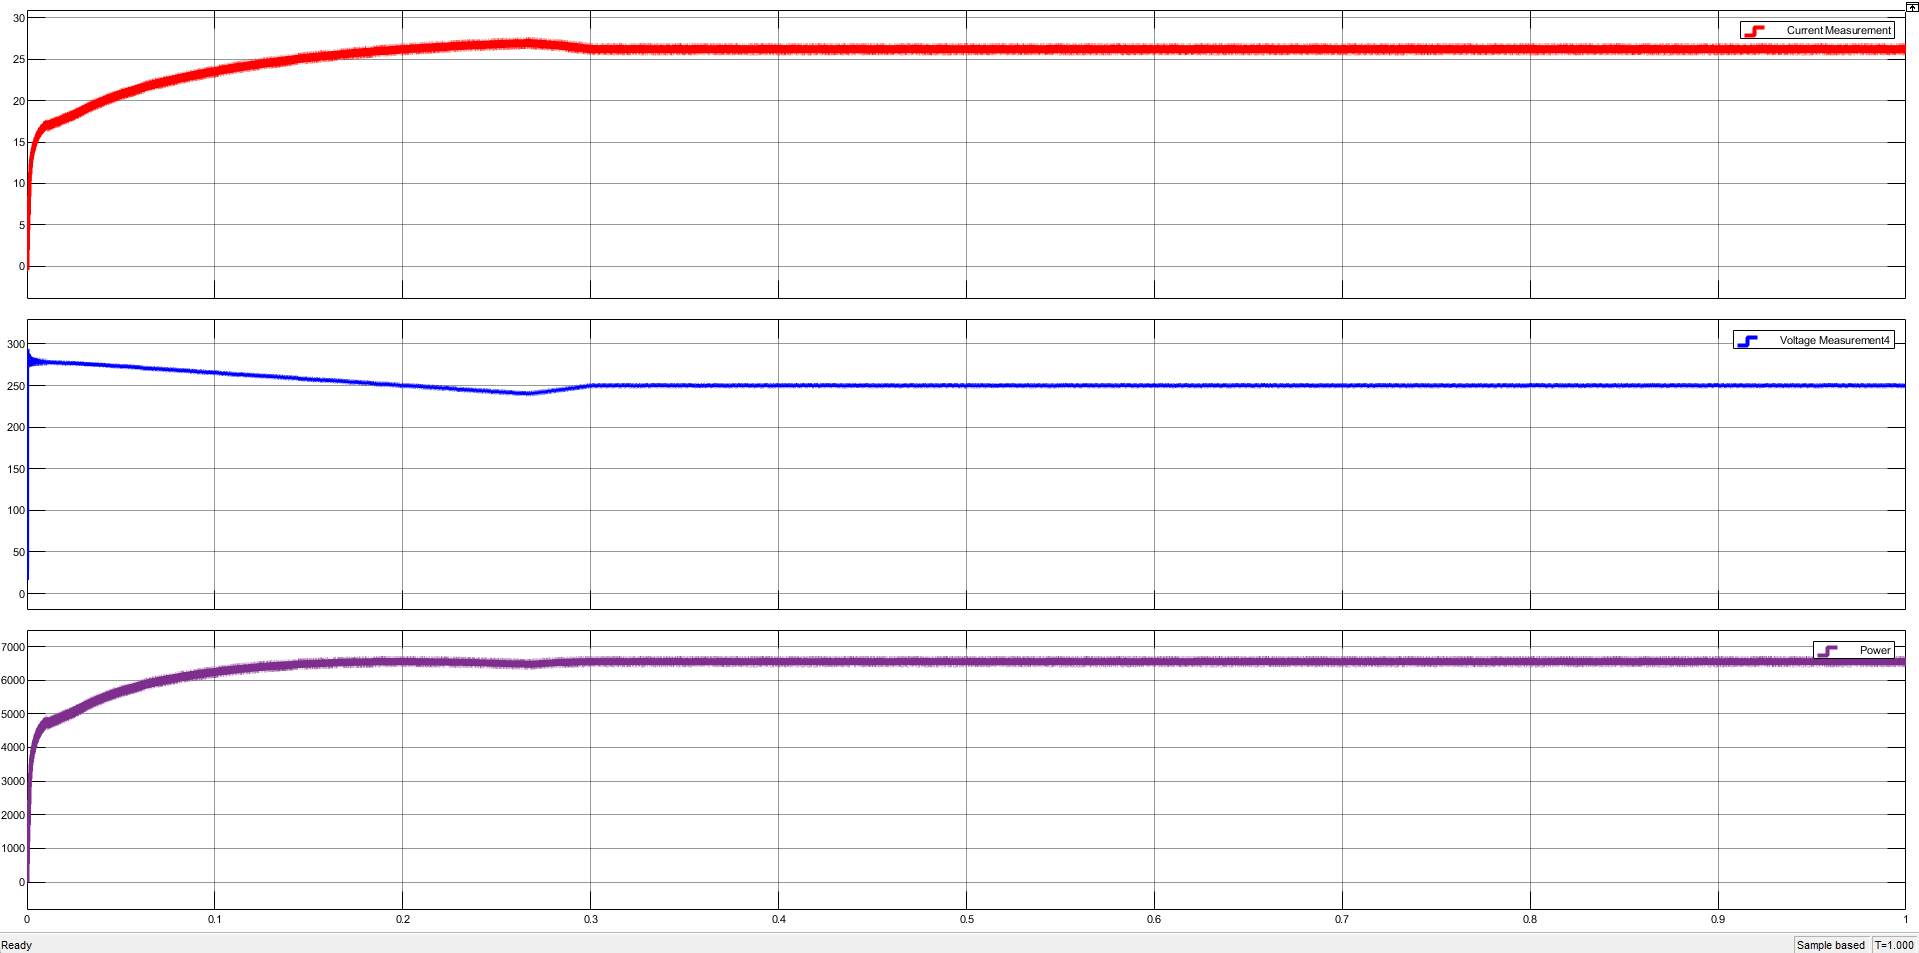
\includegraphics[width=1.1\textwidth]{Figures/5.1.15.png}
    \caption{Input current, voltage, power at 500 shading.}
    \label{fig:Input current, voltage, power at 500 shading}
\end{figure}
\begin{figure}[H]
    \centering
    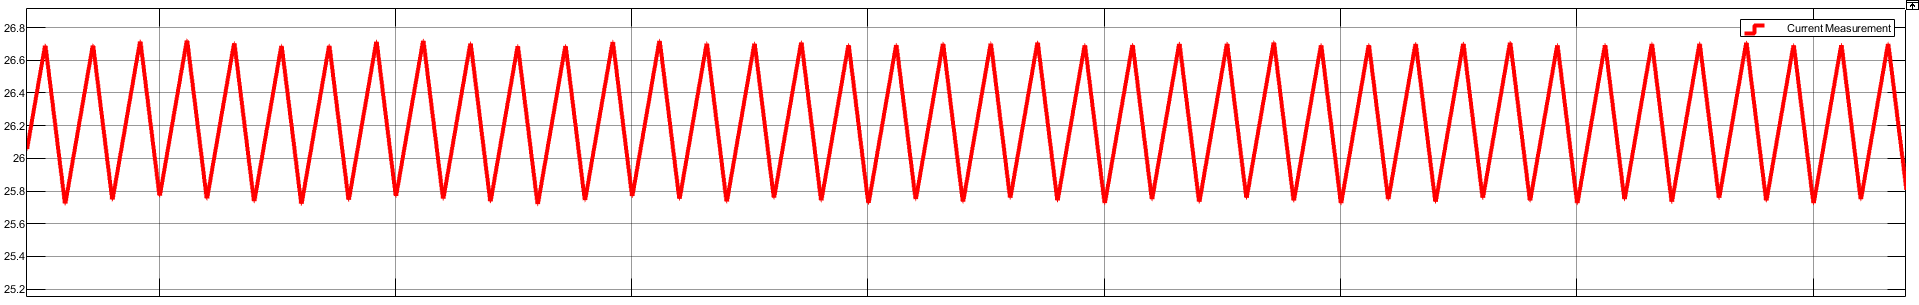
\includegraphics[width=1.1\textwidth]{Figures/5.1.16.png}
    \caption{Ripples of inductor current at 500 shading.}
    \label{fig:Ripples of inductor current at 500 shading}
\end{figure}
\begin{figure}[H]
    \centering
    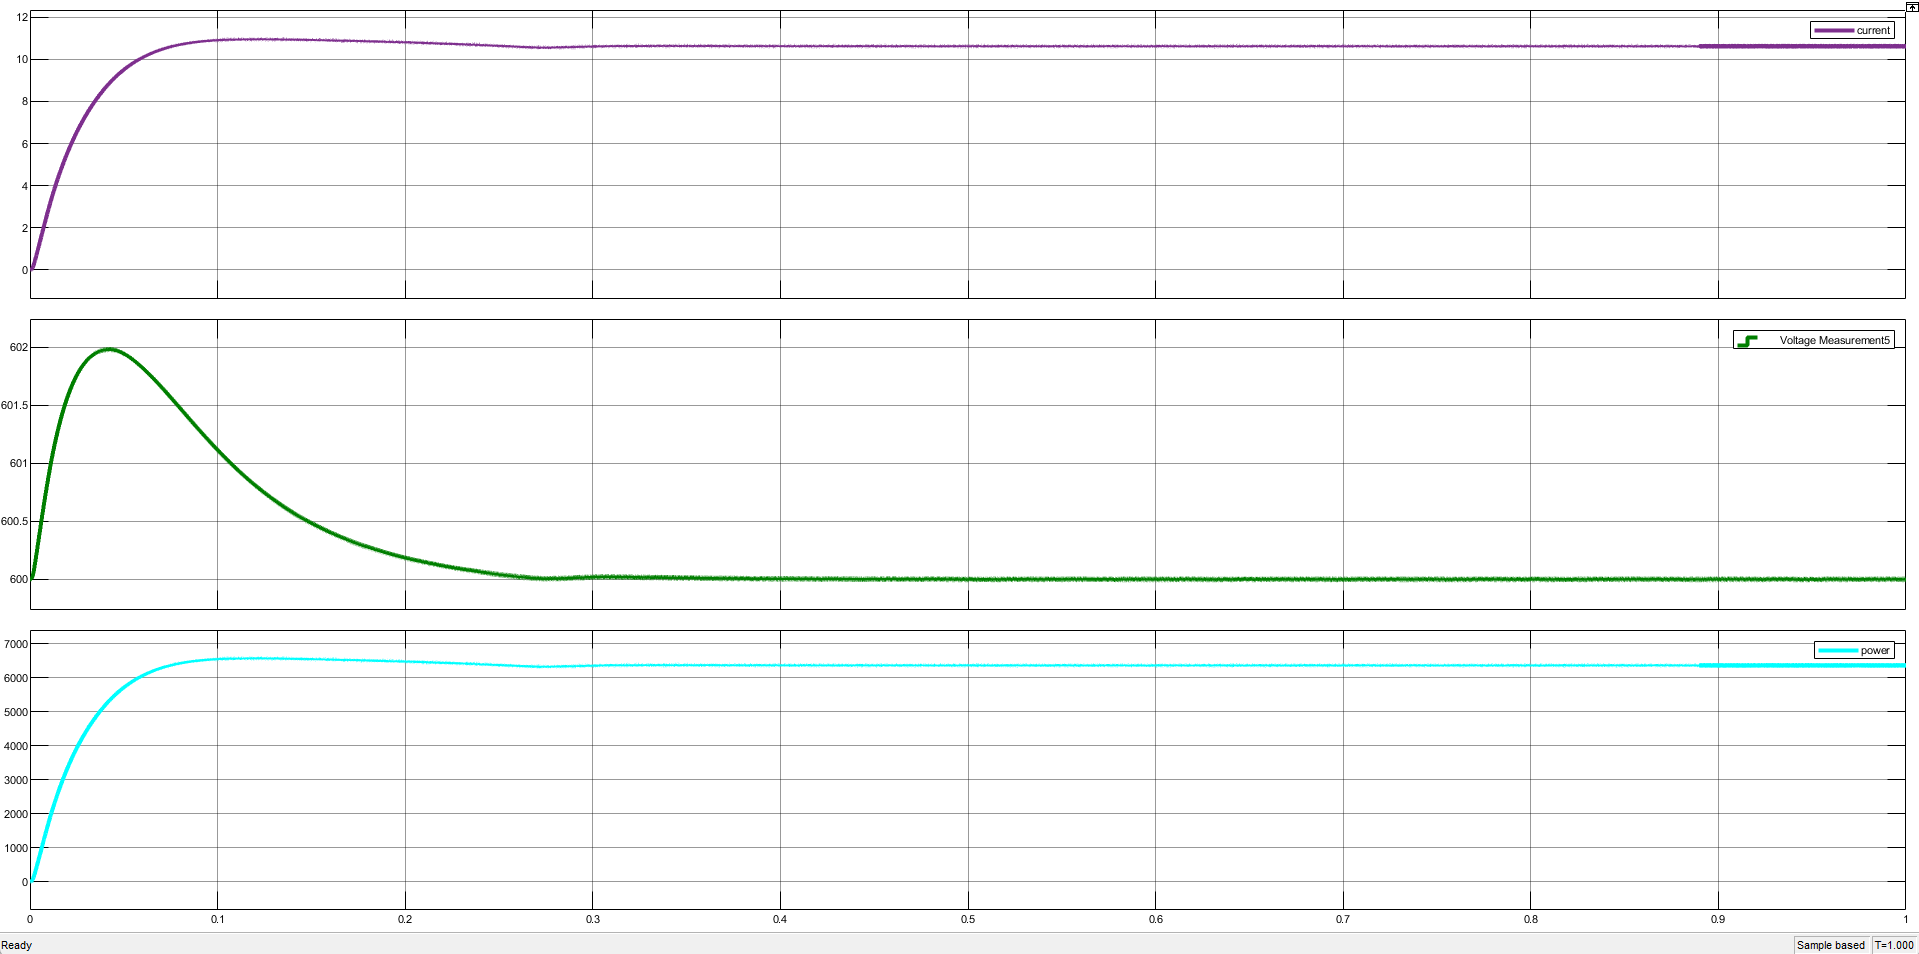
\includegraphics[width=1.1\textwidth]{Figures/5.1.17.png}
    \caption{Output current, voltage, power at 500 shading.}
    \label{fig:Output current, voltage, power at 500 shading}
\end{figure}
\subsubsection{Results of Simulation in Case of Shading (Ir = 250) at One Module}
\noindent
\begin{minipage}[t]{0.5\textwidth}
\vspace{0pt}
\begin{itemize}
  \item As shown, the output power decreases much more as the current decreases more than the current in the pervious case as Ir decreases, but the Vpv is almost constant.
  \item Dc link voltage still maintained at 600V due to closed loop with PI.
  \item Ripples of inductor current $= 22.2 - 21.4 = 0.8$\,A.
\end{itemize}
\end{minipage}
\hfill
\begin{minipage}[t]{0.4\textwidth}
\vspace{0pt}
  \centering
  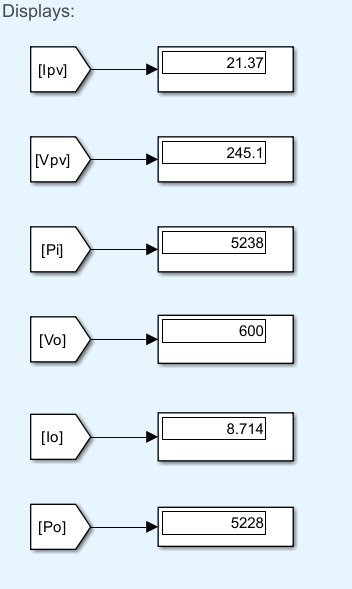
\includegraphics[width=\textwidth]{Figures/5.1.18.png}
  \captionof{figure}{Displays of central configuration at 250 shading.}
  \label{fig:Displays of central configuration at 250 shading}
\end{minipage}
\paragraph{Graphs}
\begin{figure}[H]
    \centering
    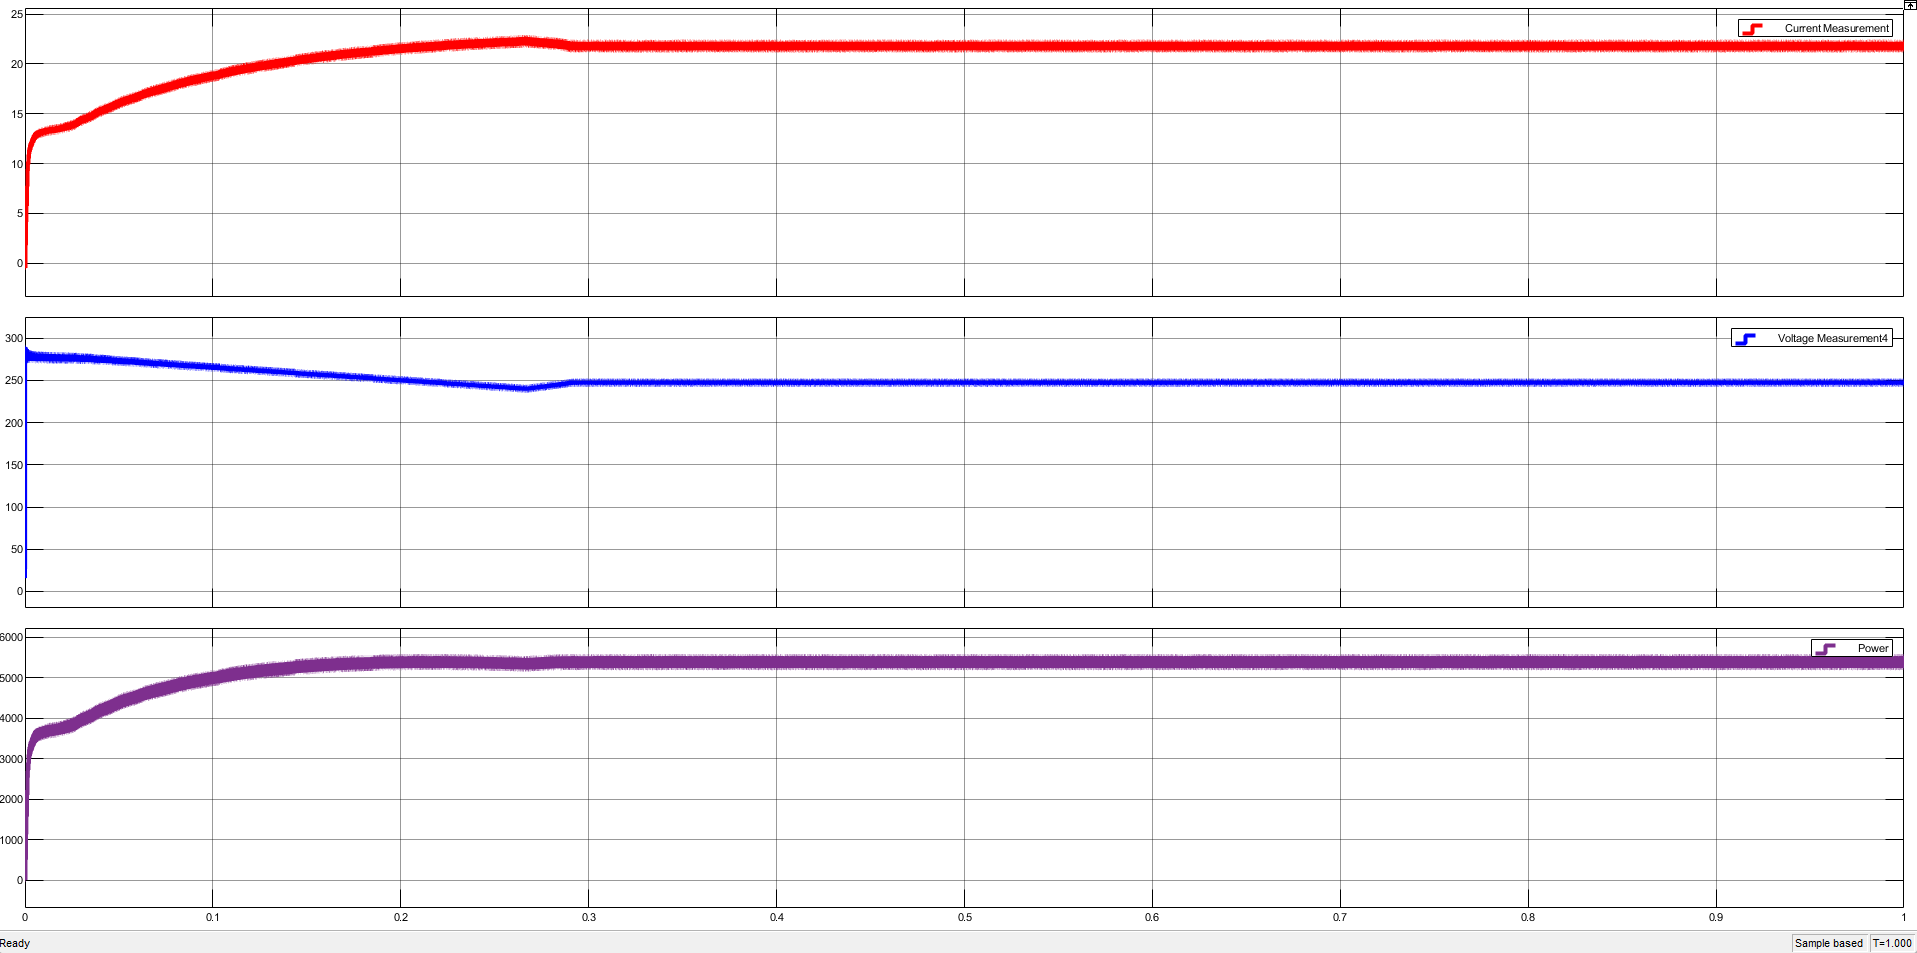
\includegraphics[width=1.1\textwidth]{Figures/5.1.19.png}
    \caption{Input current, voltage, power at 250 shading.}
    \label{fig:input current, voltage, power at 250 shading}
\end{figure}
\begin{figure}[H]
    \centering
    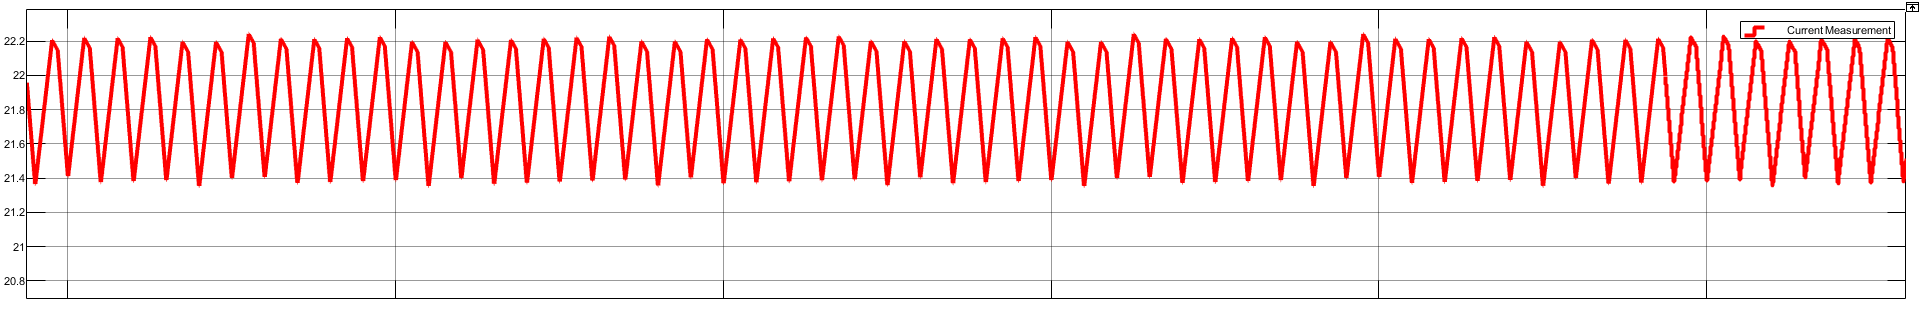
\includegraphics[width=1.1\textwidth]{Figures/5.1.20.png}
    \caption{Ripples of inductor current at 250 shading.}
    \label{fig:ripples of inductor current at 250 shading}
\end{figure}
\begin{figure}[H]
    \centering
    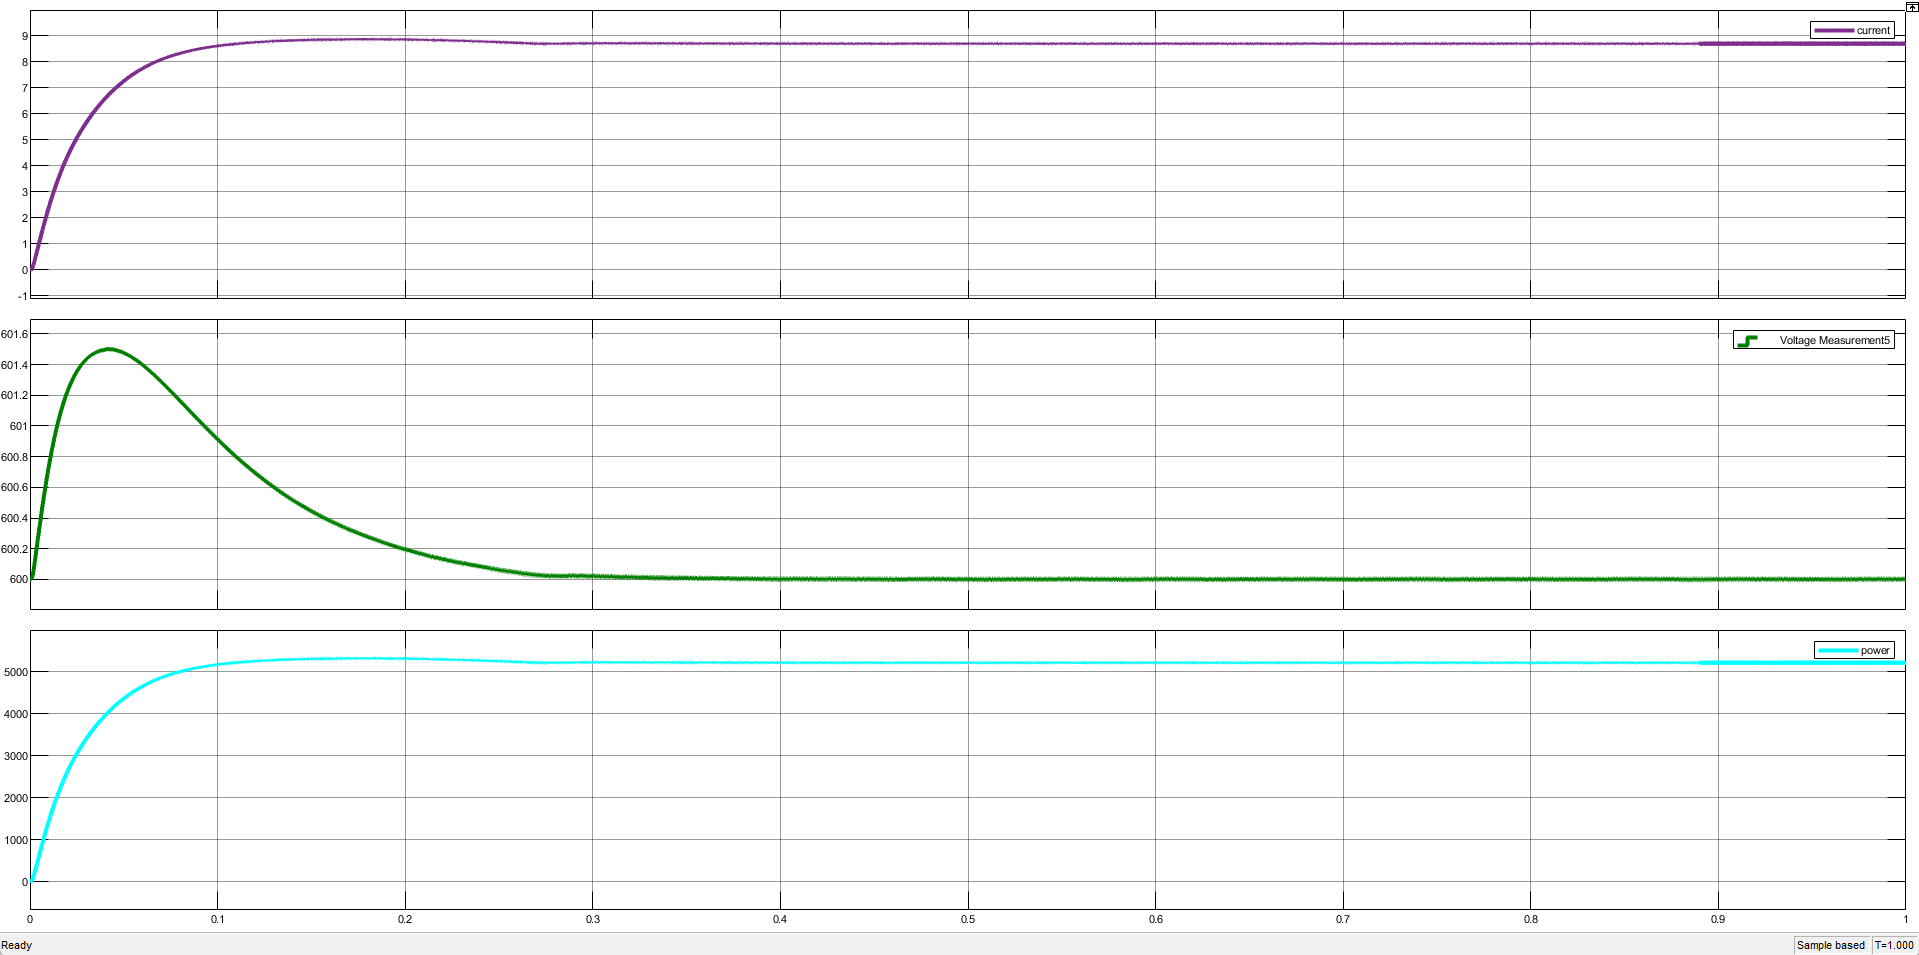
\includegraphics[width=1.1\textwidth]{Figures/5.1.21.png}
    \caption{Output current, voltage, power at 250 shading.}
    \label{fig:Output current, voltage, power at 250 shading}
\end{figure}


\subsection{String Configuration with Load}
String Array configuration is the same idea but with boost converter with each leg, all connected to the same DC link.
\begin{figure}[H]
    \centering
    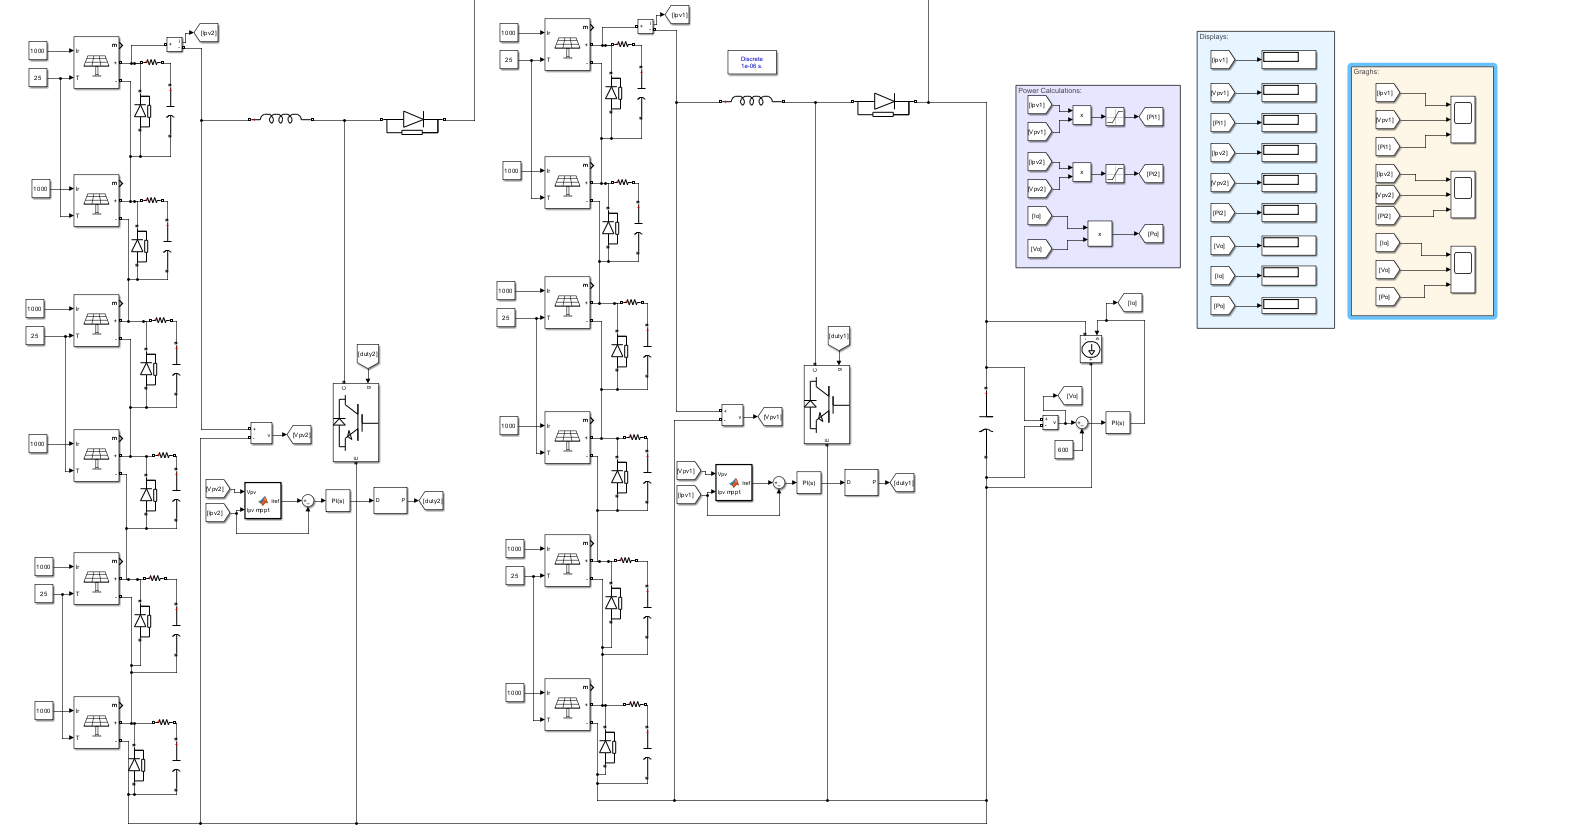
\includegraphics[width=1\textwidth]{Figures/5.1.22.png}
    \caption{String array configuration.}
    \label{fig:String array configuration}
\end{figure}
\subsubsection{Results of Simulation in Case of No Shading}
\noindent
\begin{minipage}[t]{0.5\textwidth}
\vspace{0pt}
\begin{itemize}
  \item The power is slightly less than in case of central at maximum power, the cause of this might be the more switching devices used as there are two converters instead of one.

  \item Dc link voltage still maintained at 600\,V due to closed loop with PI  
        ($K_p = 5$, $K_i = 90$). 

  \item Ripples of inductor current of string 1 $= 17.8 - 16.9 = 0.9$\,A.\
  \item Ripples of inductor current of string 2 $= 17.8 - 16.9 = 0.9$\,A.\
\end{itemize}
\end{minipage}
\hfill
\begin{minipage}[t]{0.3\textwidth}
\vspace{0pt}
  \centering
  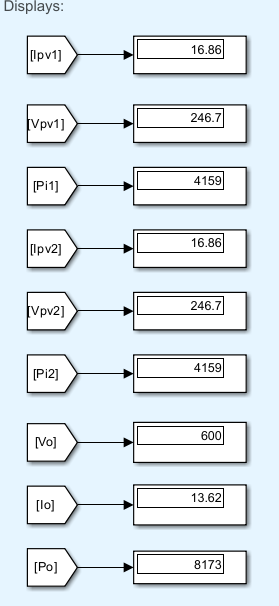
\includegraphics[width=\textwidth]{Figures/5.1.23.png}
  \captionof{figure}{Displays of string configuration at no shading.}
  \label{fig:Displays of string configuration at no shading}
\end{minipage}
\paragraph{Graphs}
\begin{figure}[H]
    \centering
    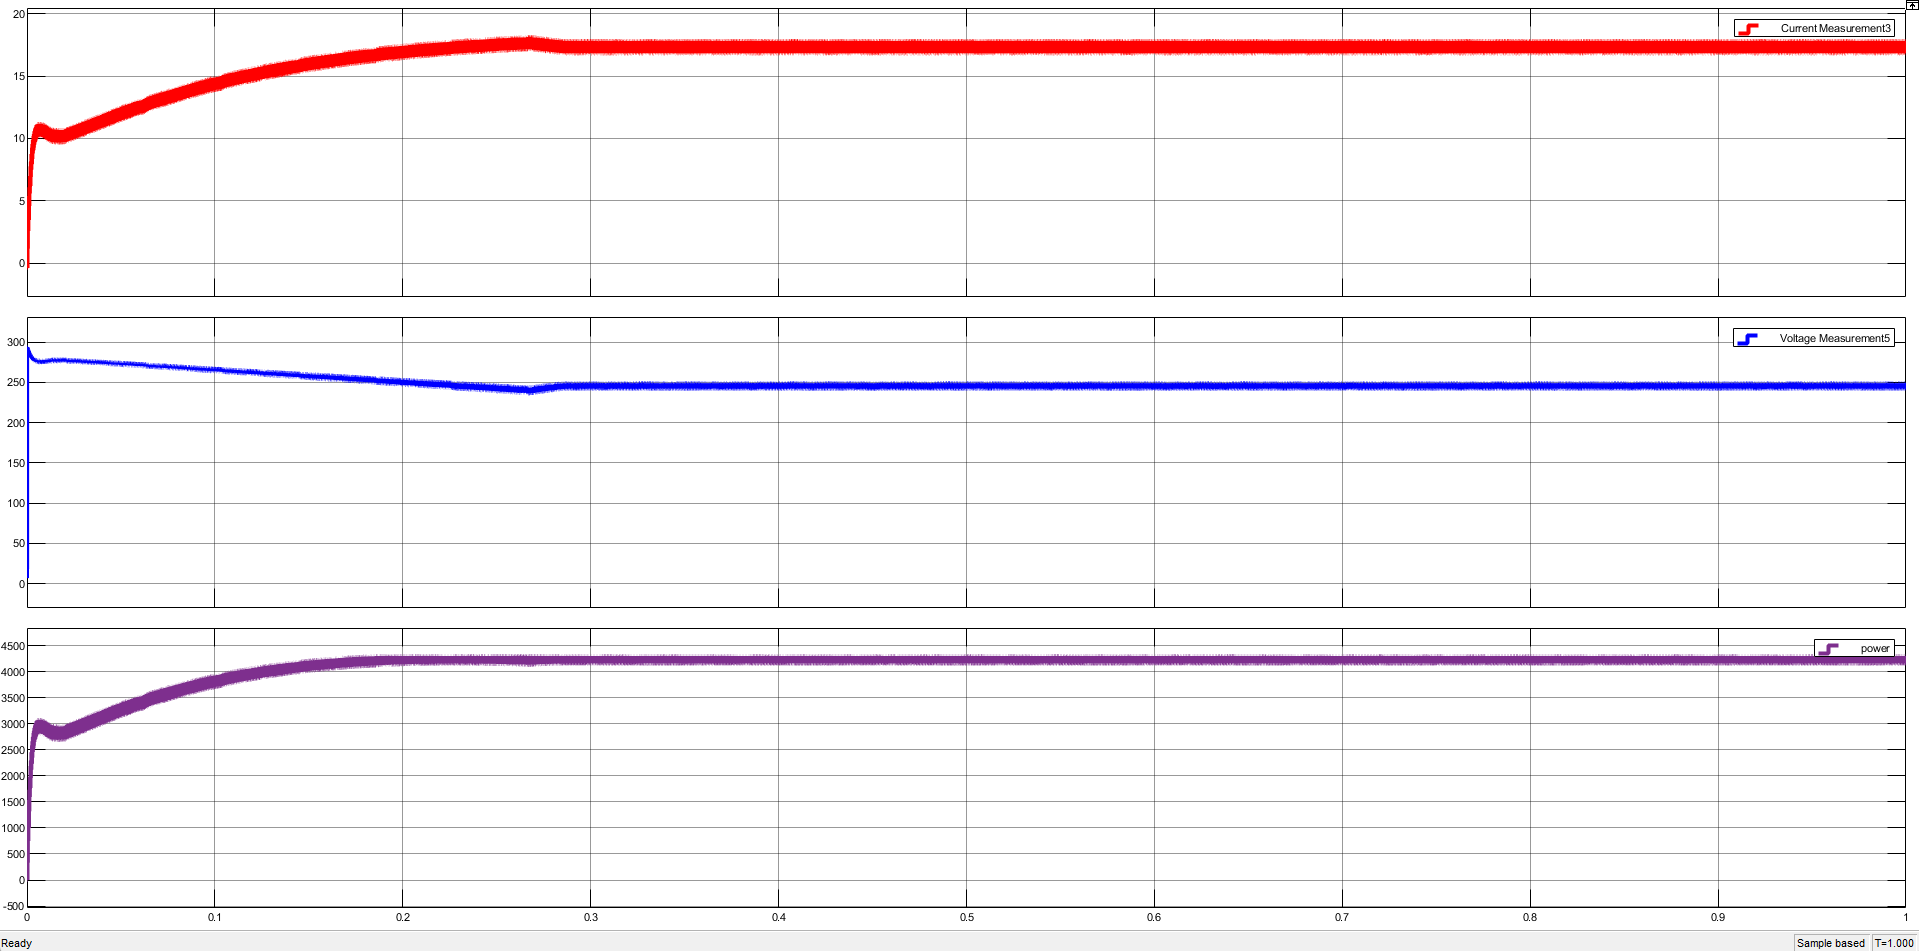
\includegraphics[width=1\textwidth]{Figures/5.1.24.png}
    \caption{Input current, voltage, power at string 1 at no shading.}
    \label{fig:input current, voltage, power at string 1 at no shading}
\end{figure}
\begin{figure}[H]
    \centering
    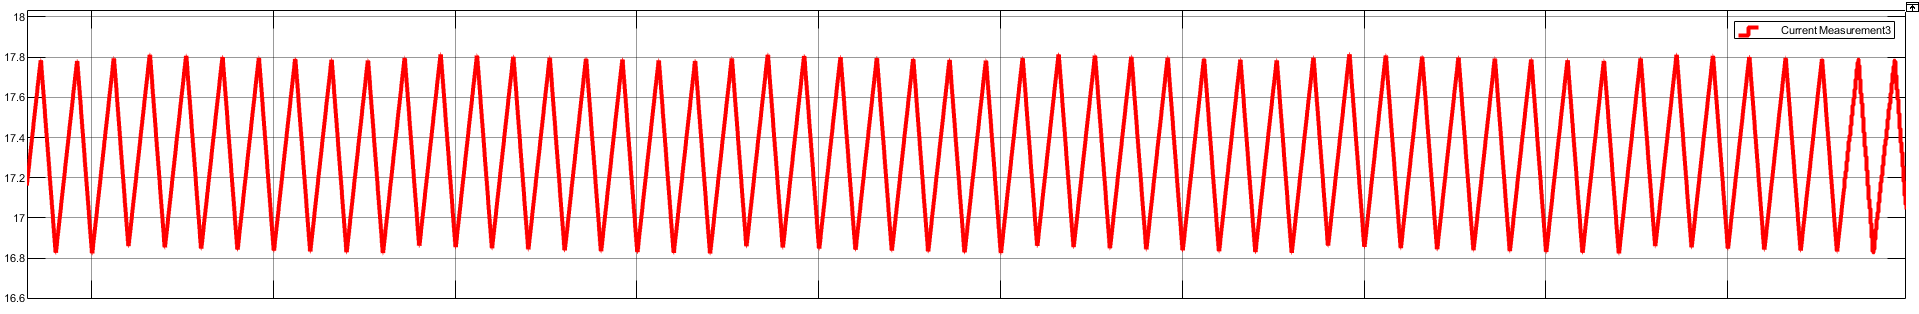
\includegraphics[width=1\textwidth]{Figures/5.1.25.png}
    \caption{Ripples of inductor current of string 1 at no shading.}
    \label{fig:Ripples of inductor current of string 1 at no shading}
\end{figure}
\begin{figure}[H]
    \centering
    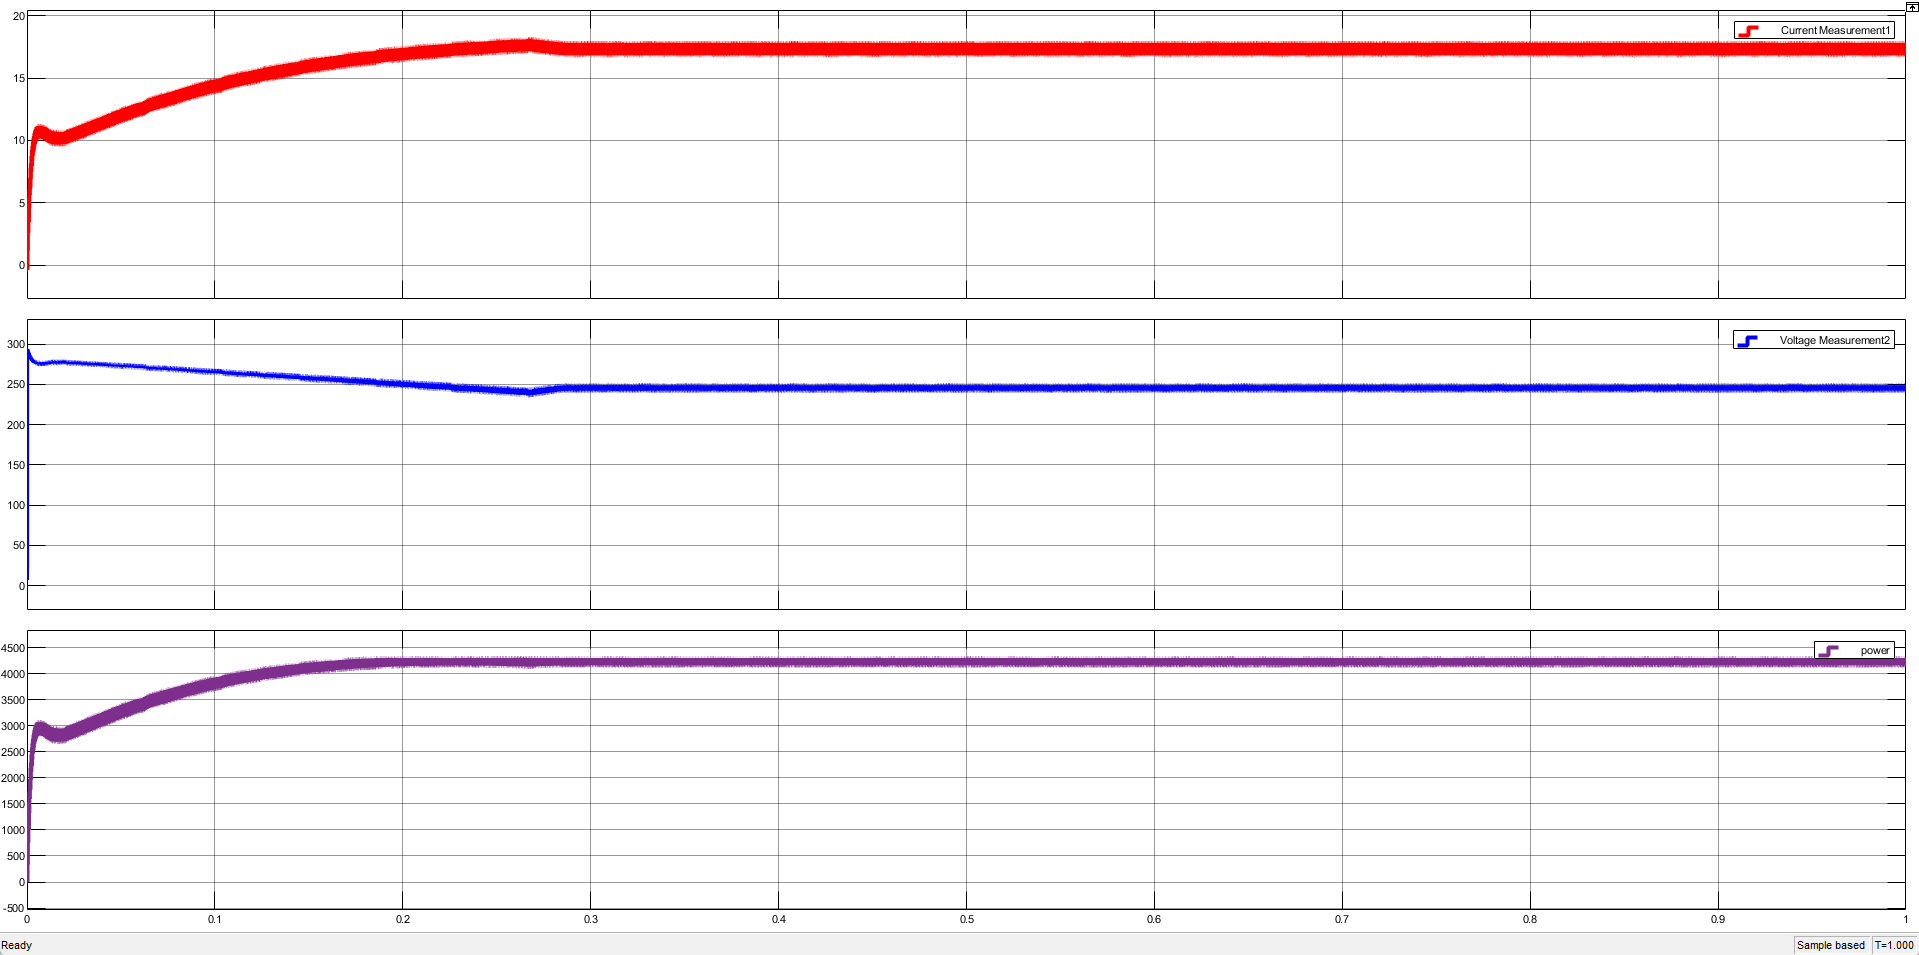
\includegraphics[width=1\textwidth]{Figures/5.1.26.png}
    \caption{Input current, voltage, power at string 2 at no shading.}
    \label{fig:input current, voltage, power at string 2 at no shading}
\end{figure}
\begin{figure}[H]
    \centering
    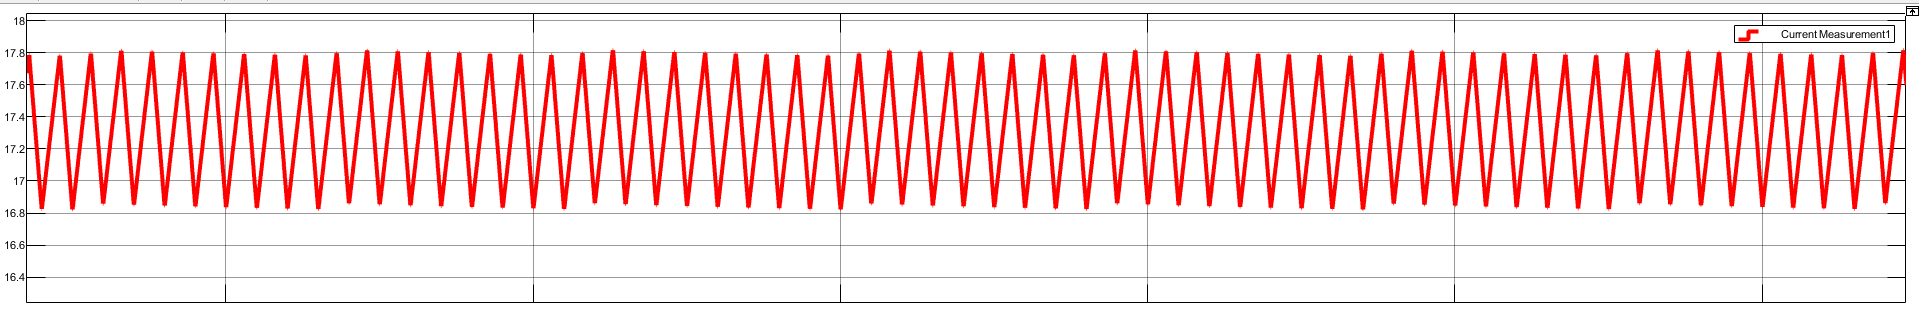
\includegraphics[width=1\textwidth]{Figures/5.1.27.png}
    \caption{Ripples of inductor current of string 2 at no shading.}
    \label{fig:ripples of inductor current of string 2 at no shading}
\end{figure}
\begin{figure}[H]
    \centering
    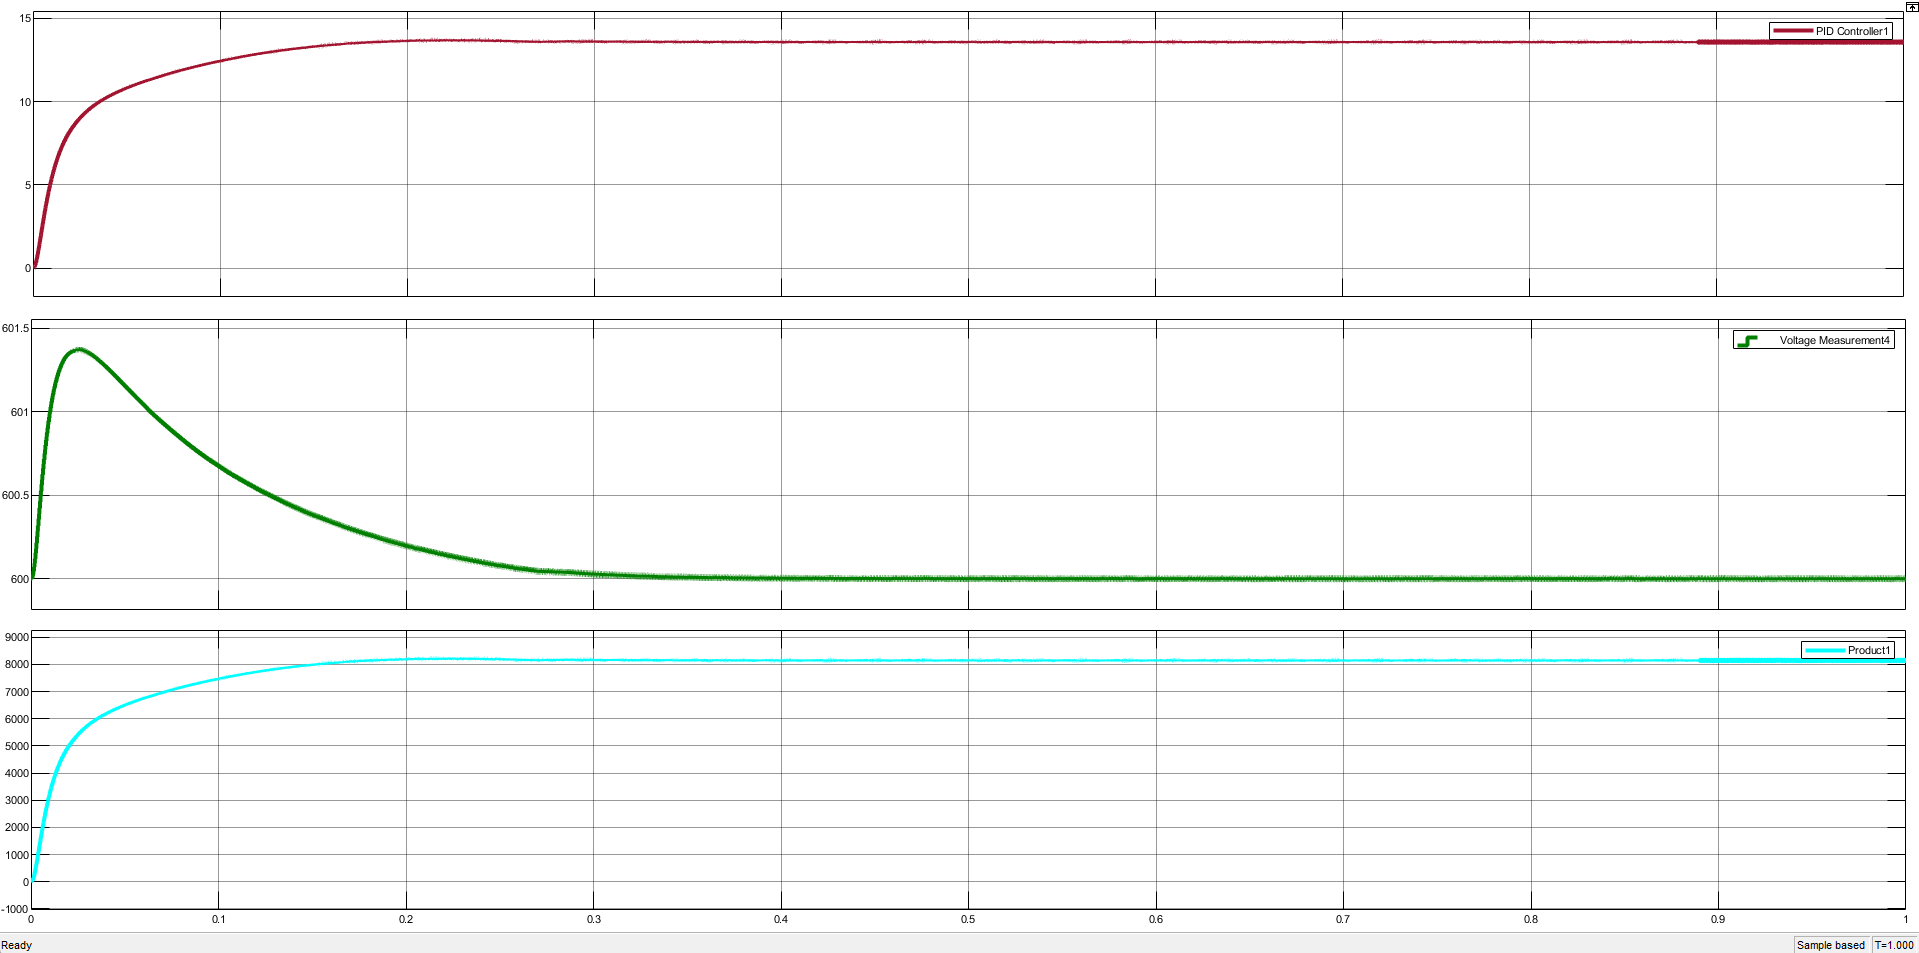
\includegraphics[width=1\textwidth]{Figures/5.1.28.png}
    \caption{Output current, voltage, power at no shading.}
    \label{fig:Output current, voltage, power at no shading}
\end{figure}

\subsubsection{Results of Simulation in Case of Shading (Ir = 800) at One Module at One String}
\noindent
\begin{minipage}[t]{0.5\textwidth}
\vspace{0pt}
\begin{itemize}
  \item As shown, the output power decreases as the current decreases only in the string that has shaded module, but the other string is unshaded, so it outputs the max power.
\item As shown, the output power in string configuration is more than the output power in central configuration and this is the key difference between them and why is string is better in shading.
  \item Dc link voltage still maintained at 600\,V due to closed loop with PI.  

  \item Ripples of inductor current of string 1 $= 17.8 - 16.9 = 0.9$\,A.\
  \item Ripples of inductor current of string 2 $= 15 - 14 = 1$\,A.\
\end{itemize}
\end{minipage}
\hfill
\begin{minipage}[t]{0.3\textwidth}
\vspace{0pt}
  \centering
  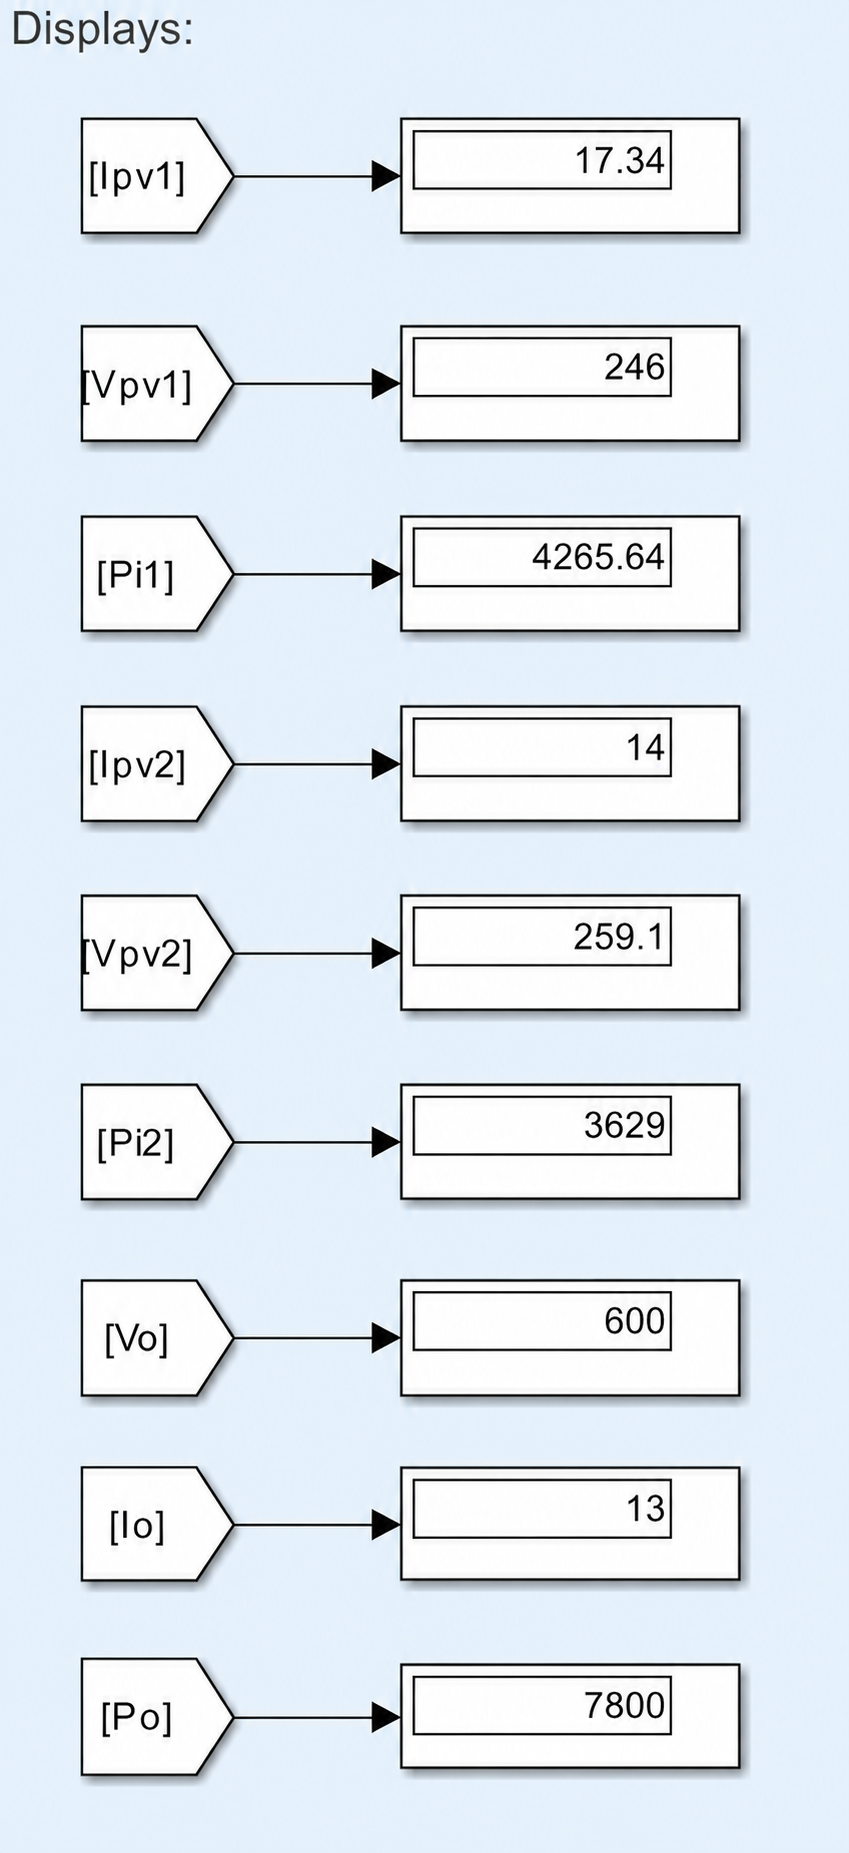
\includegraphics[width=\textwidth]{Figures/5.1.70.png}
  \captionof{figure}{Displays of string configuration at 800 shading.}
  \label{fig:Displays of string configuration at 800 shading}
\end{minipage}
\paragraph{Graphs}
\begin{figure}[H]
    \centering
    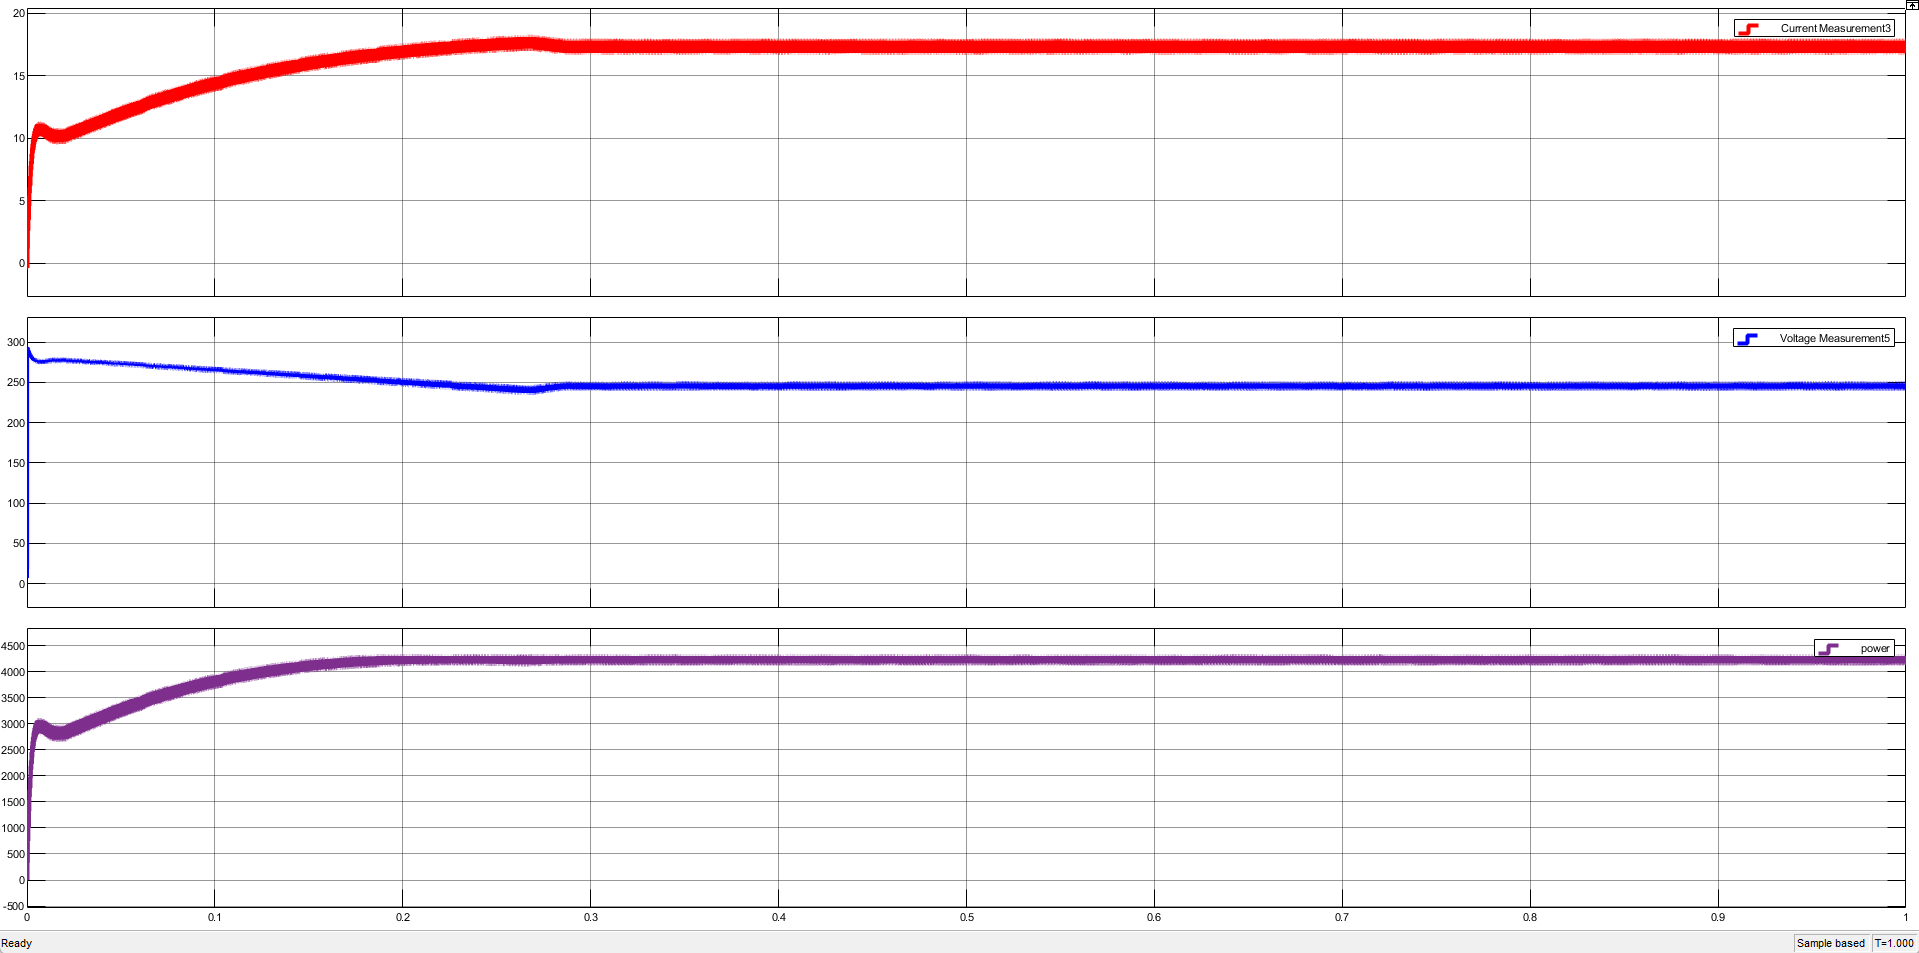
\includegraphics[width=1\textwidth]{Figures/5.1.30.png}
    \caption{Input current, voltage, power at string 1 at 800 shading.}
    \label{fig:input current, voltage, power at string 1 at 800 shading}
\end{figure}
\begin{figure}[H]
    \centering
    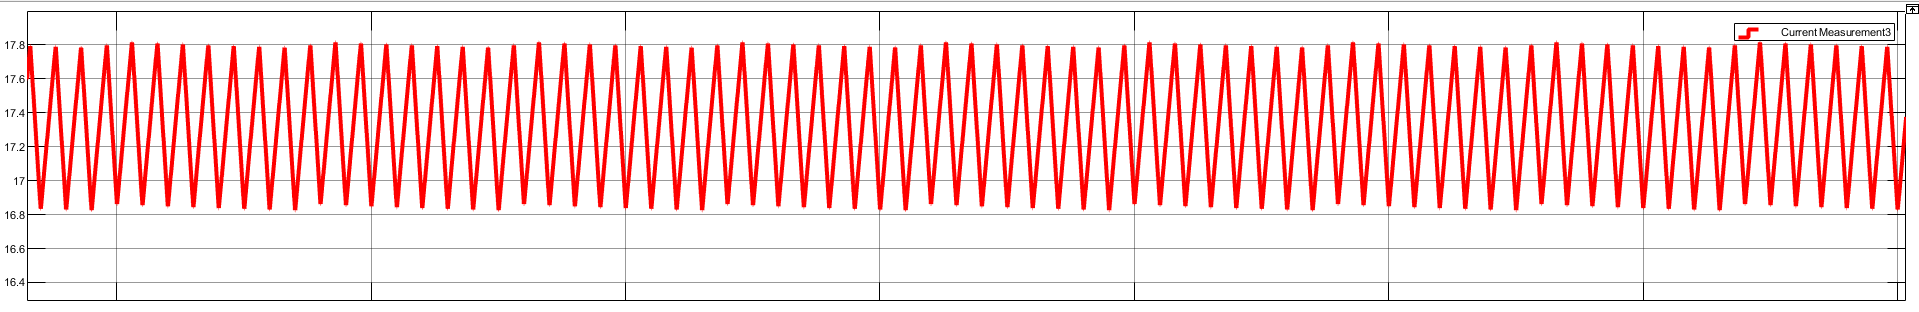
\includegraphics[width=1\textwidth]{Figures/5.1.31.png}
    \caption{Ripples of inductor current of string 1 at 800 shading.}
    \label{fig:ripples of inductor current of string 1 at 800 shading}
\end{figure}
\begin{figure}[H]
    \centering
    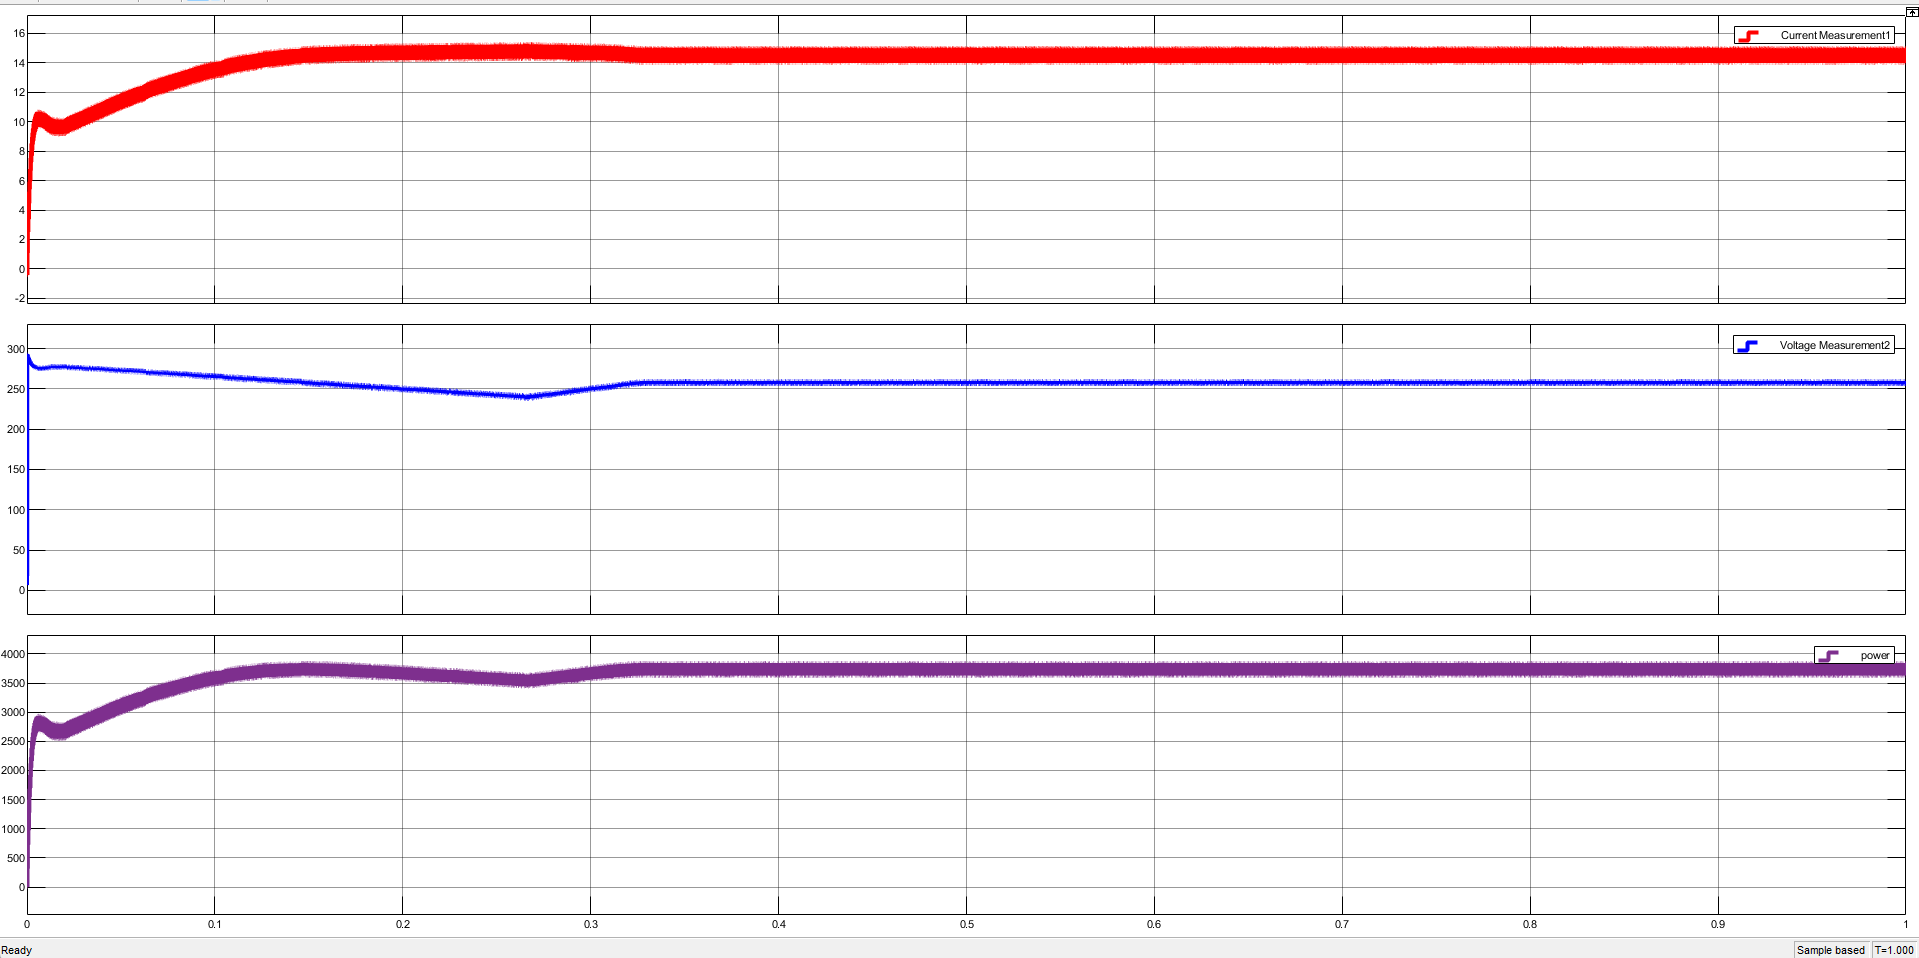
\includegraphics[width=1\textwidth]{Figures/5.1.32.png}
    \caption{Input current, voltage, power at string 2 at 800 shading.}
    \label{fig:input current, voltage, power at string 2 at 800 shading}
\end{figure}
\begin{figure}[H]
    \centering
    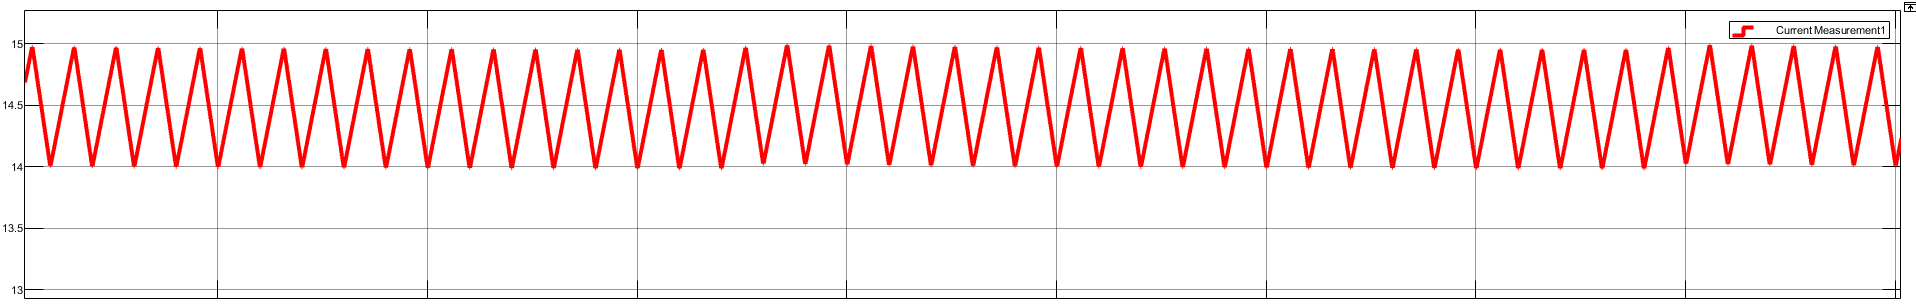
\includegraphics[width=1\textwidth]{Figures/5.1.33.png}
    \caption{Ripples of inductor current of string 2 at 800 shading.}
    \label{fig:ripples of inductor current of string 2 at 800 shading}
\end{figure}
\begin{figure}[H]
    \centering
    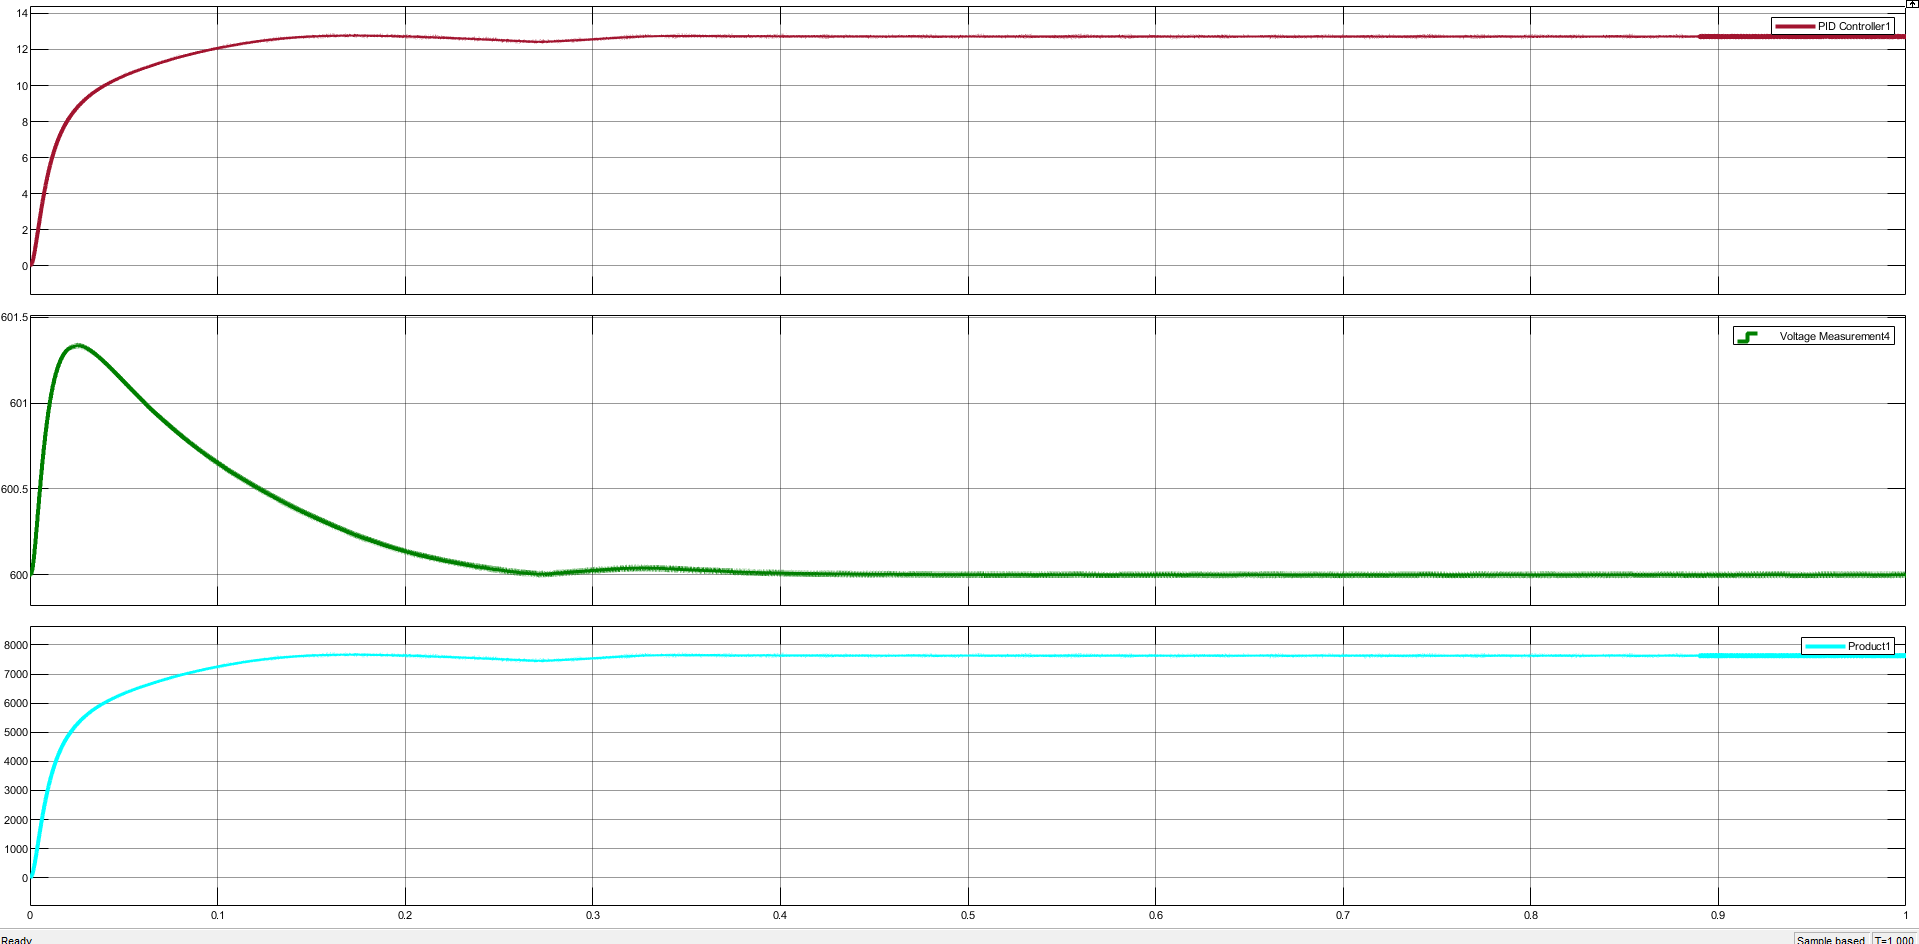
\includegraphics[width=1\textwidth]{Figures/5.1.34.png}
    \caption{Output current, voltage, power at 800 shading.}
    \label{fig:Output current, voltage, power at 800 shading}
\end{figure}

\subsubsection{Results of Simulation in Case of Shading (Ir = 500) at One Module at One String}
\noindent
\begin{minipage}[t]{0.5\textwidth}
\vspace{0pt}
\begin{itemize}
  \item As shown, the output power decreases as the current decreases only in the string that has shaded module, but the other string is unshaded, so it outputs the max power.
  \item As shown, the output power in string configuration is more than the output power in central configuration and this is the key difference between them and why is string is better in shading.
  \item Dc link voltage still maintained at 600\,V due to closed loop with PI.  

  \item Ripples of inductor current of string 1 $= 17.5 - 16.6 = 0.9$\,A.\
  \item Ripples of inductor current of string 2 $= 9.7 - 8.8 = 0.9$\,A.\
\end{itemize}
\end{minipage}
\hfill
\begin{minipage}[t]{0.3\textwidth}
\vspace{0pt}
  \centering
  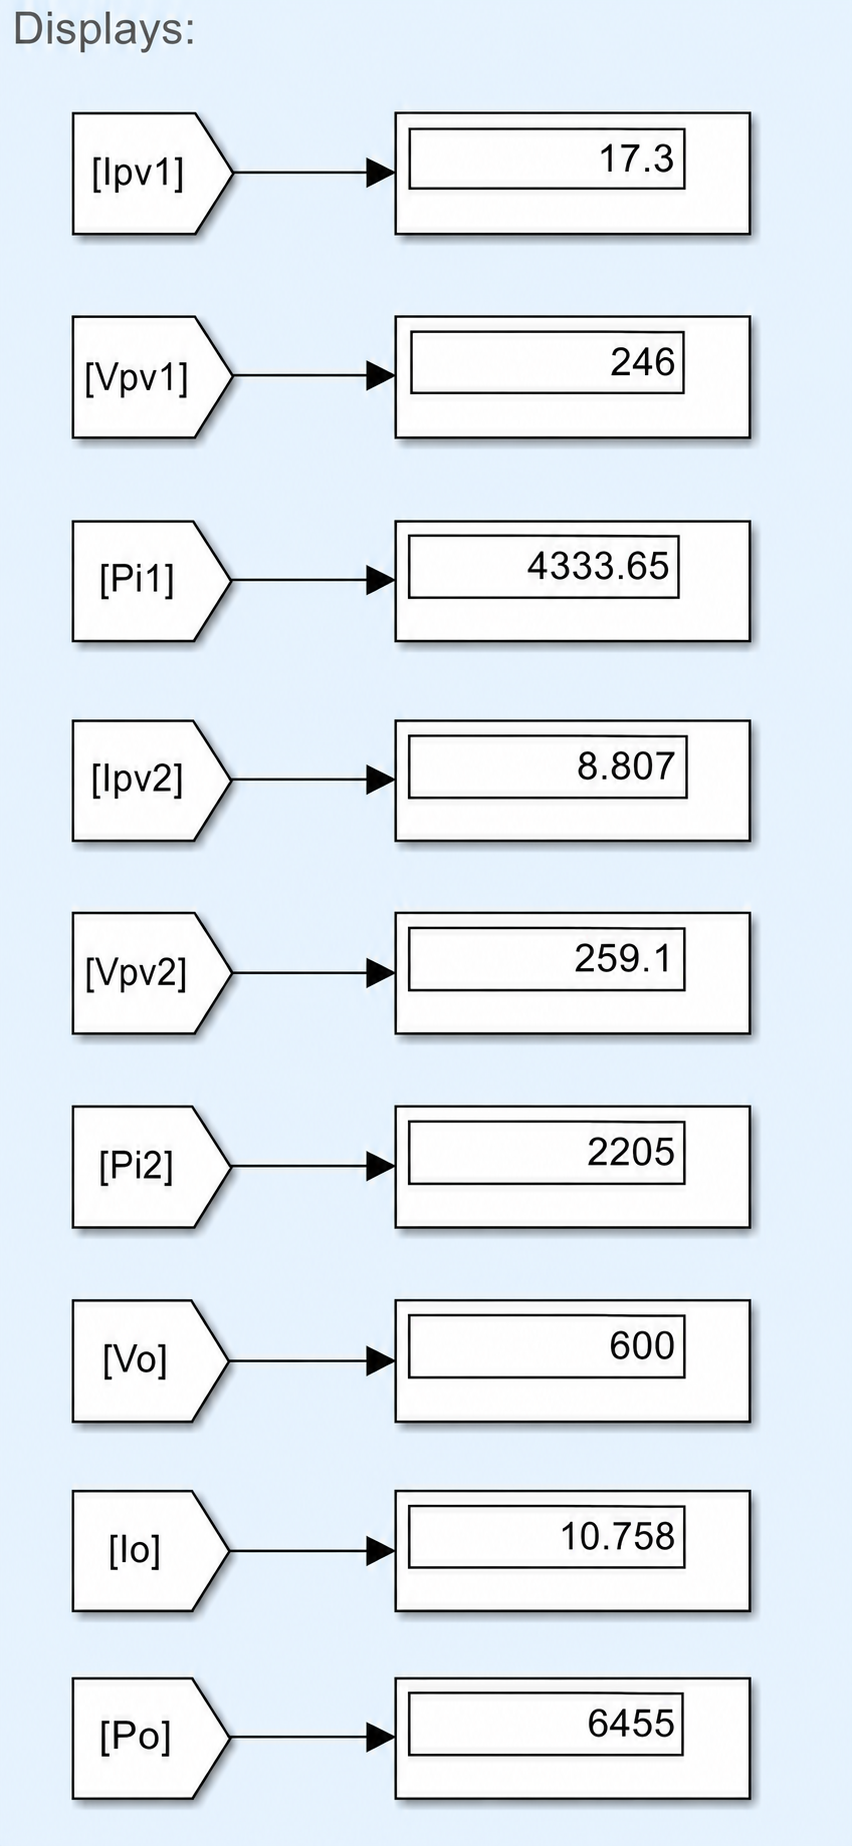
\includegraphics[width=\textwidth]{Figures/5.1.71.png}
  \captionof{figure}{Displays of string configuration at 500 shading.}
  \label{fig:Displays of string configuration at 500 shading}
\end{minipage}
\paragraph{Graphs}
\begin{figure}[H]
    \centering
    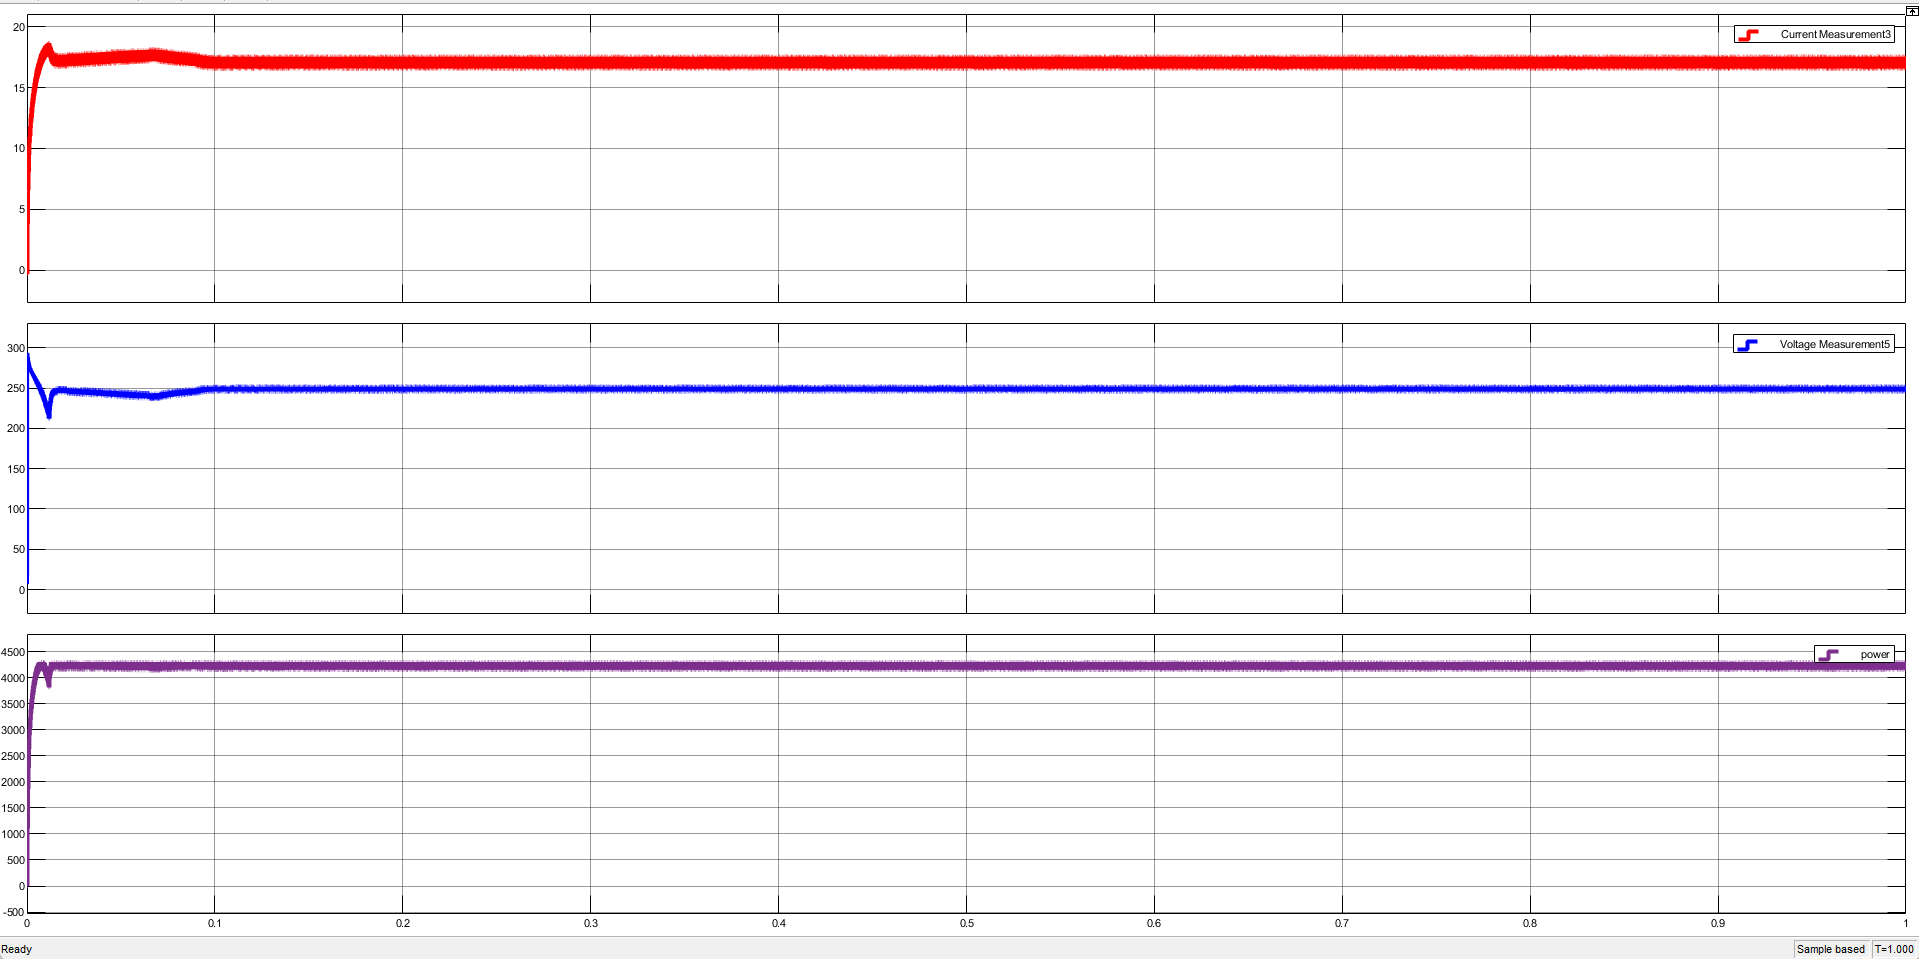
\includegraphics[width=1\textwidth]{Figures/5.1.36.png}
    \caption{Input current, voltage, power at string 1 at 500 shading.}
    \label{fig:input current, voltage, power at string 1 at 500 shading}
\end{figure}
\begin{figure}[H]
    \centering
    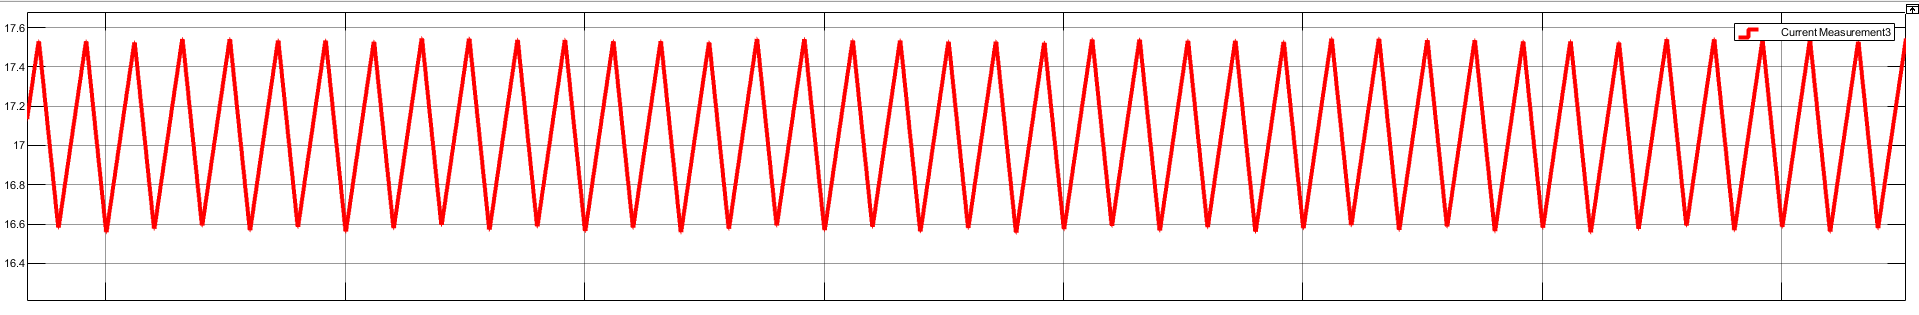
\includegraphics[width=1\textwidth]{Figures/5.1.37.png}
    \caption{Ripples of inductor current of string 1 at 500 shading.}
    \label{fig:ripples of inductor current of string 1 at 500 shading}
\end{figure}
\begin{figure}[H]
    \centering
    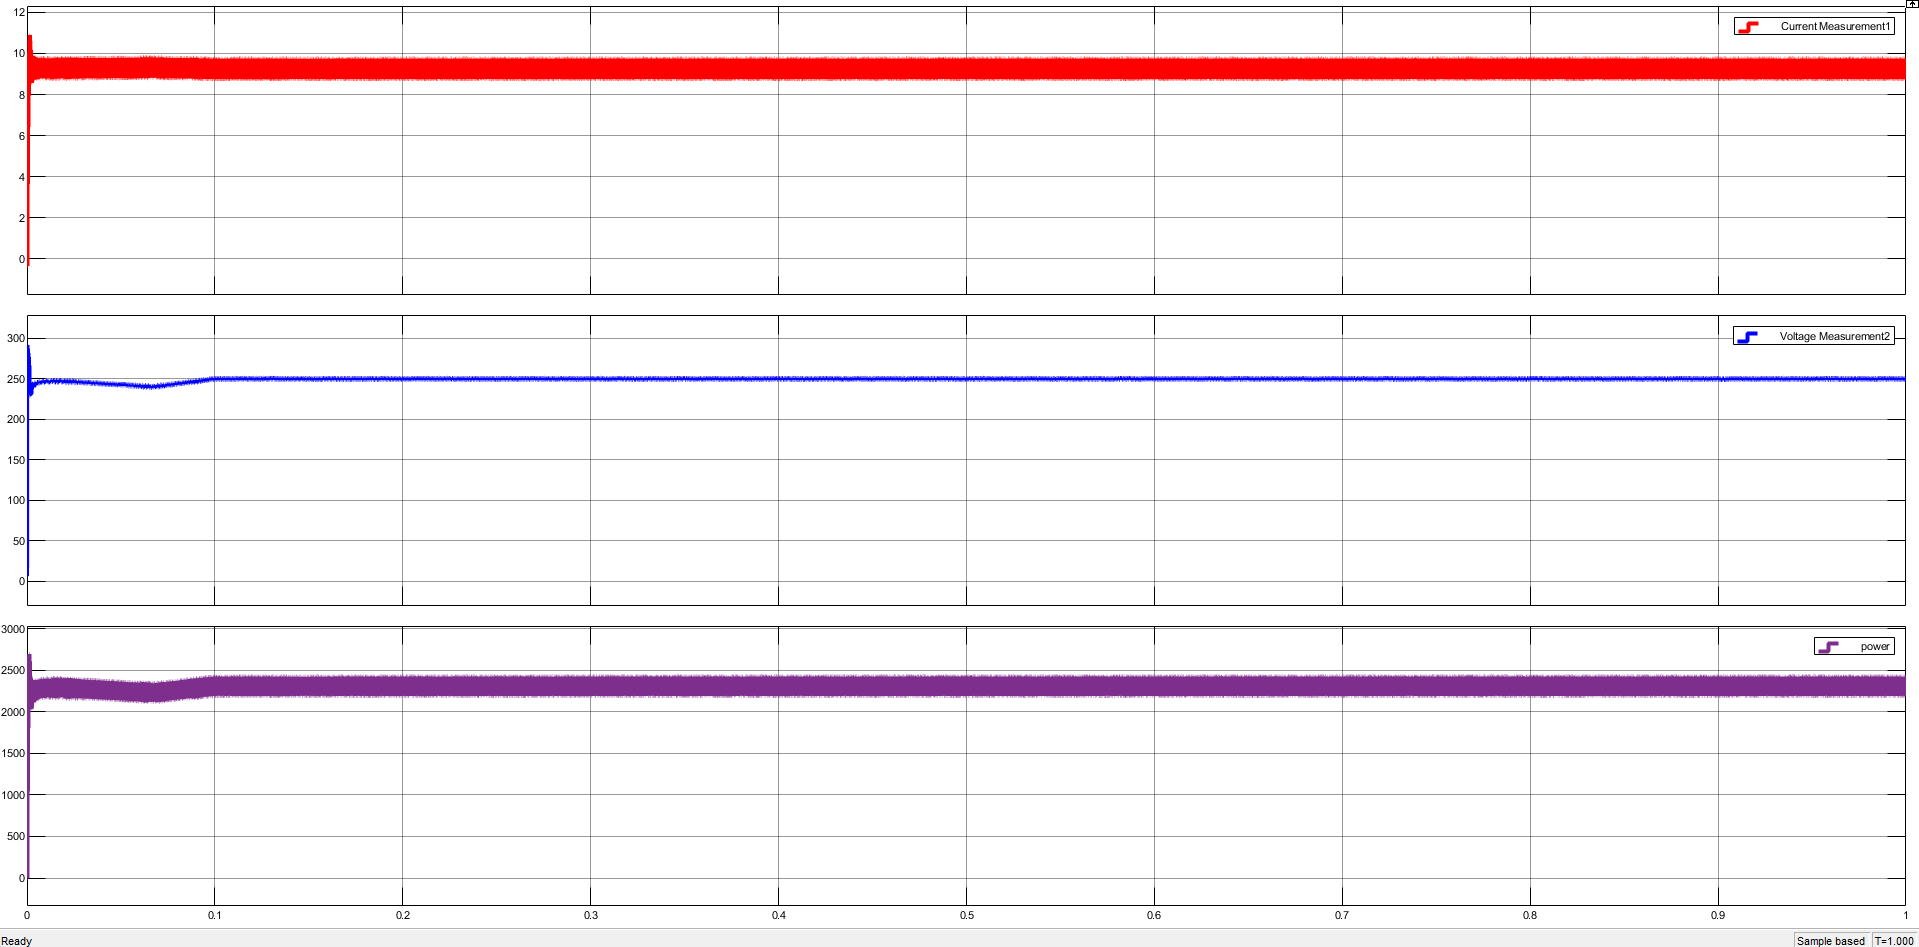
\includegraphics[width=1\textwidth]{Figures/5.1.38.png}
    \caption{Input current, voltage, power at string 2 at 500 shading.}
    \label{fig:input current, voltage, power at string 2 at 500 shading}
\end{figure}
\begin{figure}[H]
    \centering
    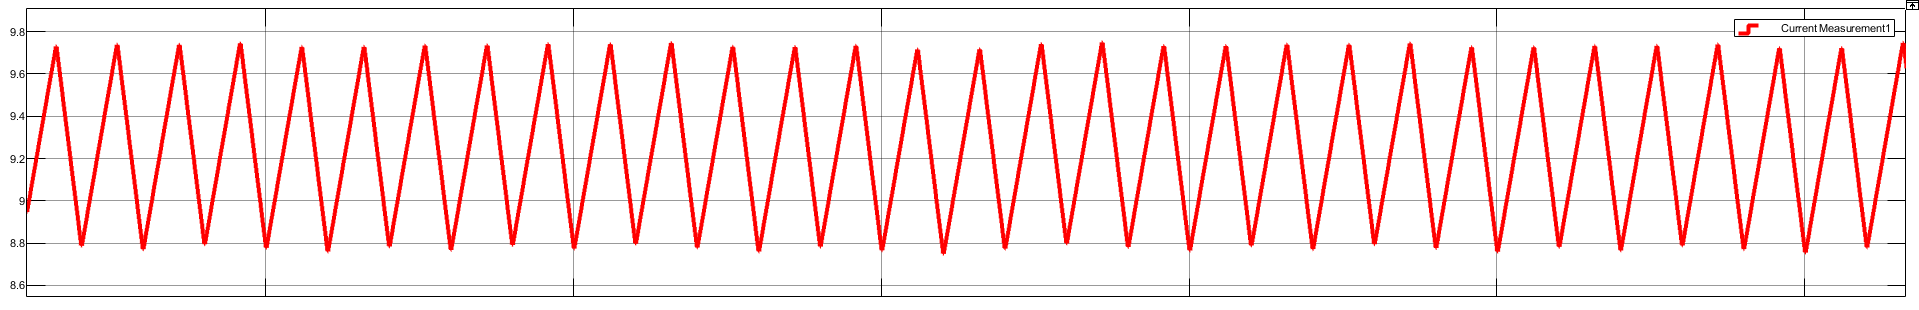
\includegraphics[width=1\textwidth]{Figures/5.1.39.png}
    \caption{Ripples of inductor current of string 2 at 500 shading.}
    \label{fig:ripples of inductor current of string 2 at 500 shading}
\end{figure}
\begin{figure}[H]
    \centering
    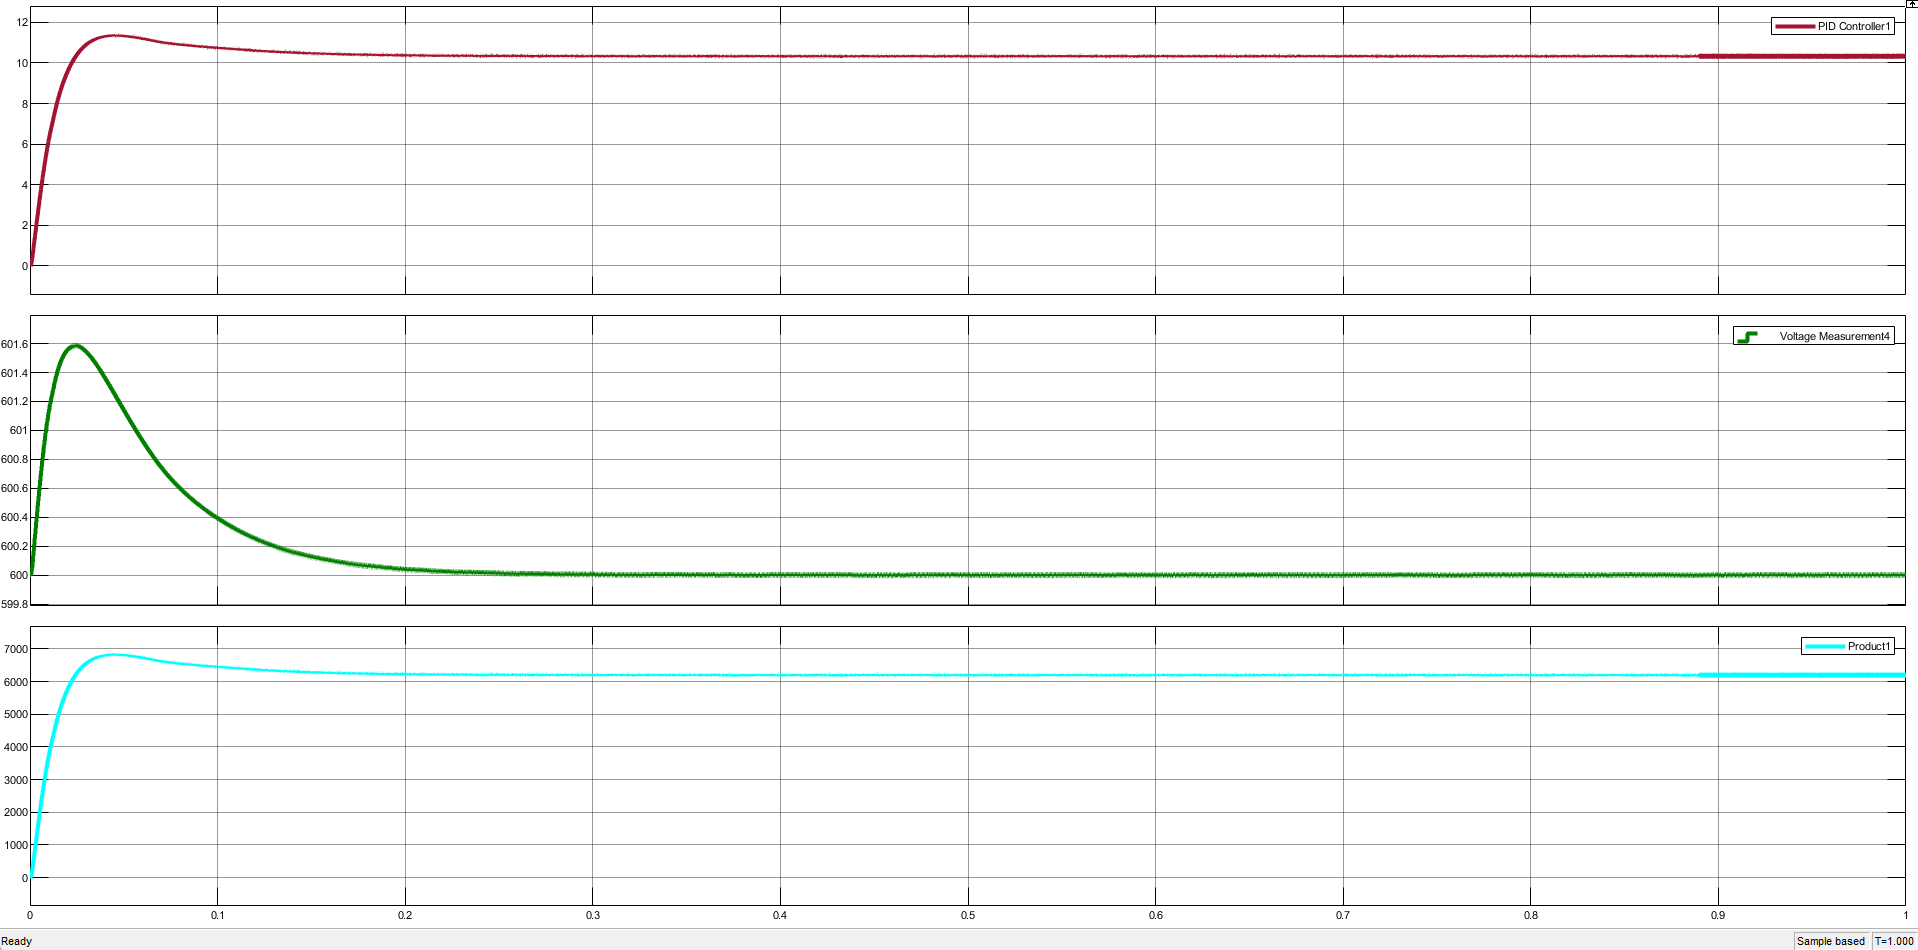
\includegraphics[width=1\textwidth]{Figures/5.1.40.png}
    \caption{Output current, voltage, power at 500 shading.}
    \label{fig:Output current, voltage, power at 500 shading}
\end{figure}

\subsubsection{Results of Simulation in Case of Shading (Ir = 250) at One Module at One String}
\noindent
\begin{minipage}[t]{0.5\textwidth}
\vspace{0pt}
\begin{itemize}
  \item As shown, the output power decreases as the current decreases only in the string that has shaded module, but the other string is unshaded, so it outputs the max power.
  \item As shown, the output power in string configuration is more than the output power in central configuration and this is the key difference between them and why is string is better in shading.
  \item Dc link voltage still maintained at 600\,V due to closed loop with PI.  

  \item Ripples of inductor current of string 1 $= 17.5 - 16.6 = 0.9$\,A.\
  \item Ripples of inductor current of string 2 $= 5.1 - 4.2 = 0.9$\,A.\
\end{itemize}
\end{minipage}
\hfill
\begin{minipage}[t]{0.3\textwidth}
\vspace{0pt}
  \centering
  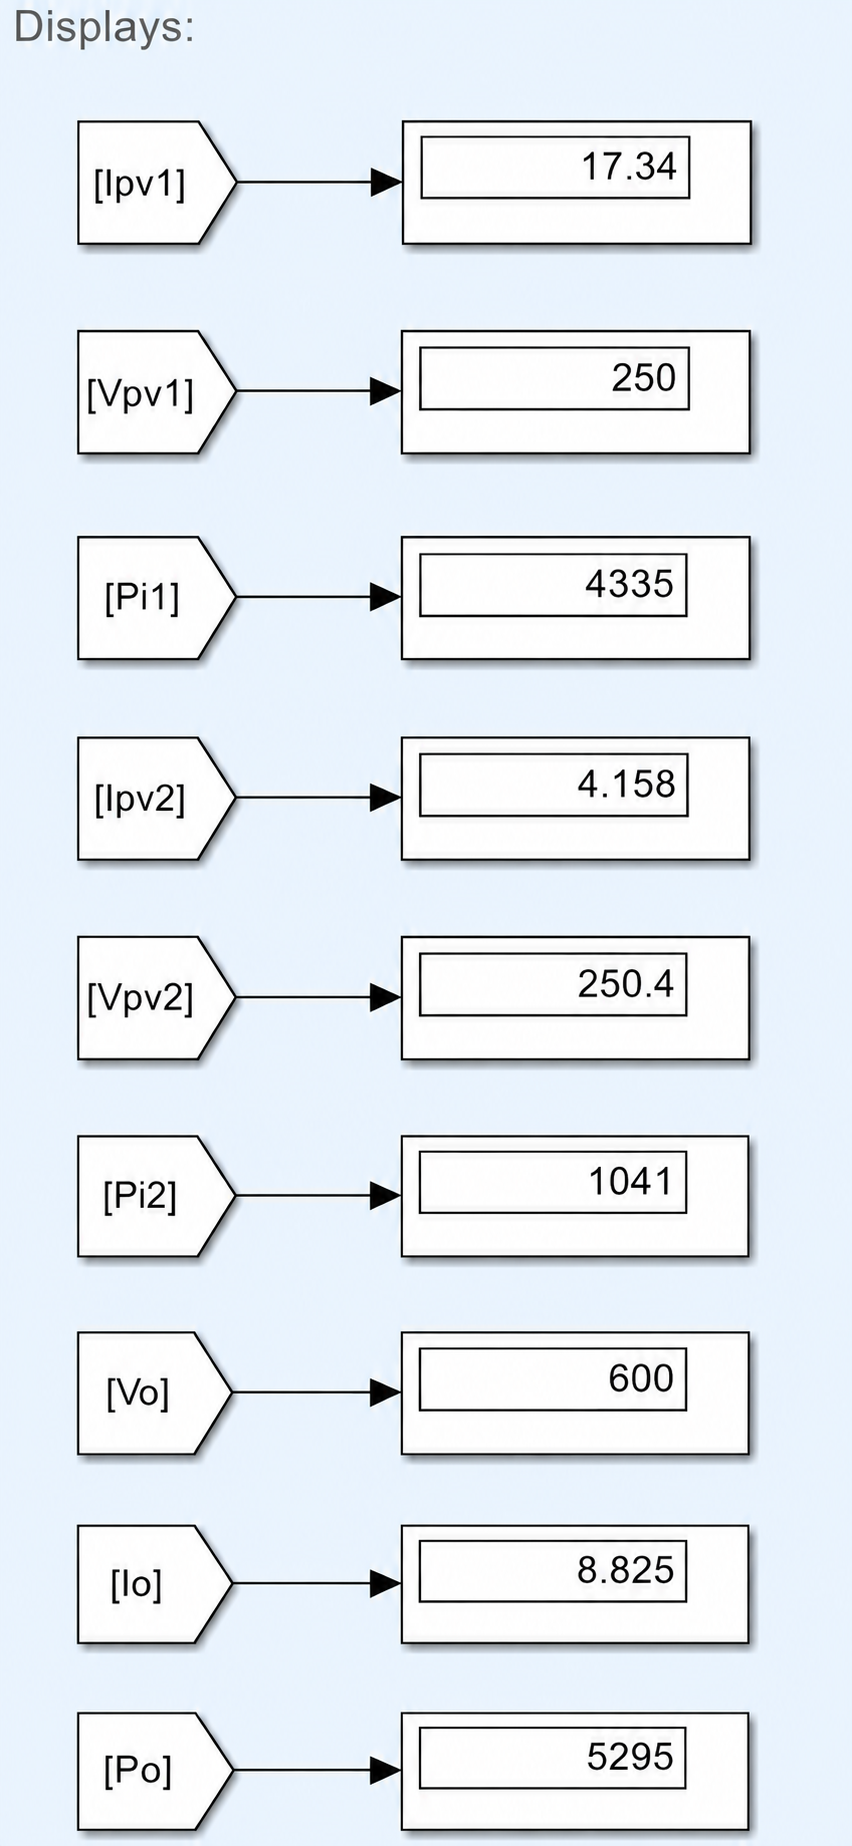
\includegraphics[width=\textwidth]{Figures/5.1.72.png}
  \captionof{figure}{Displays of string configuration at 250 shading.}
  \label{fig:Displays of string configuration at 250 shading}
\end{minipage}
\paragraph{Graphs}
\begin{figure}[H]
    \centering
    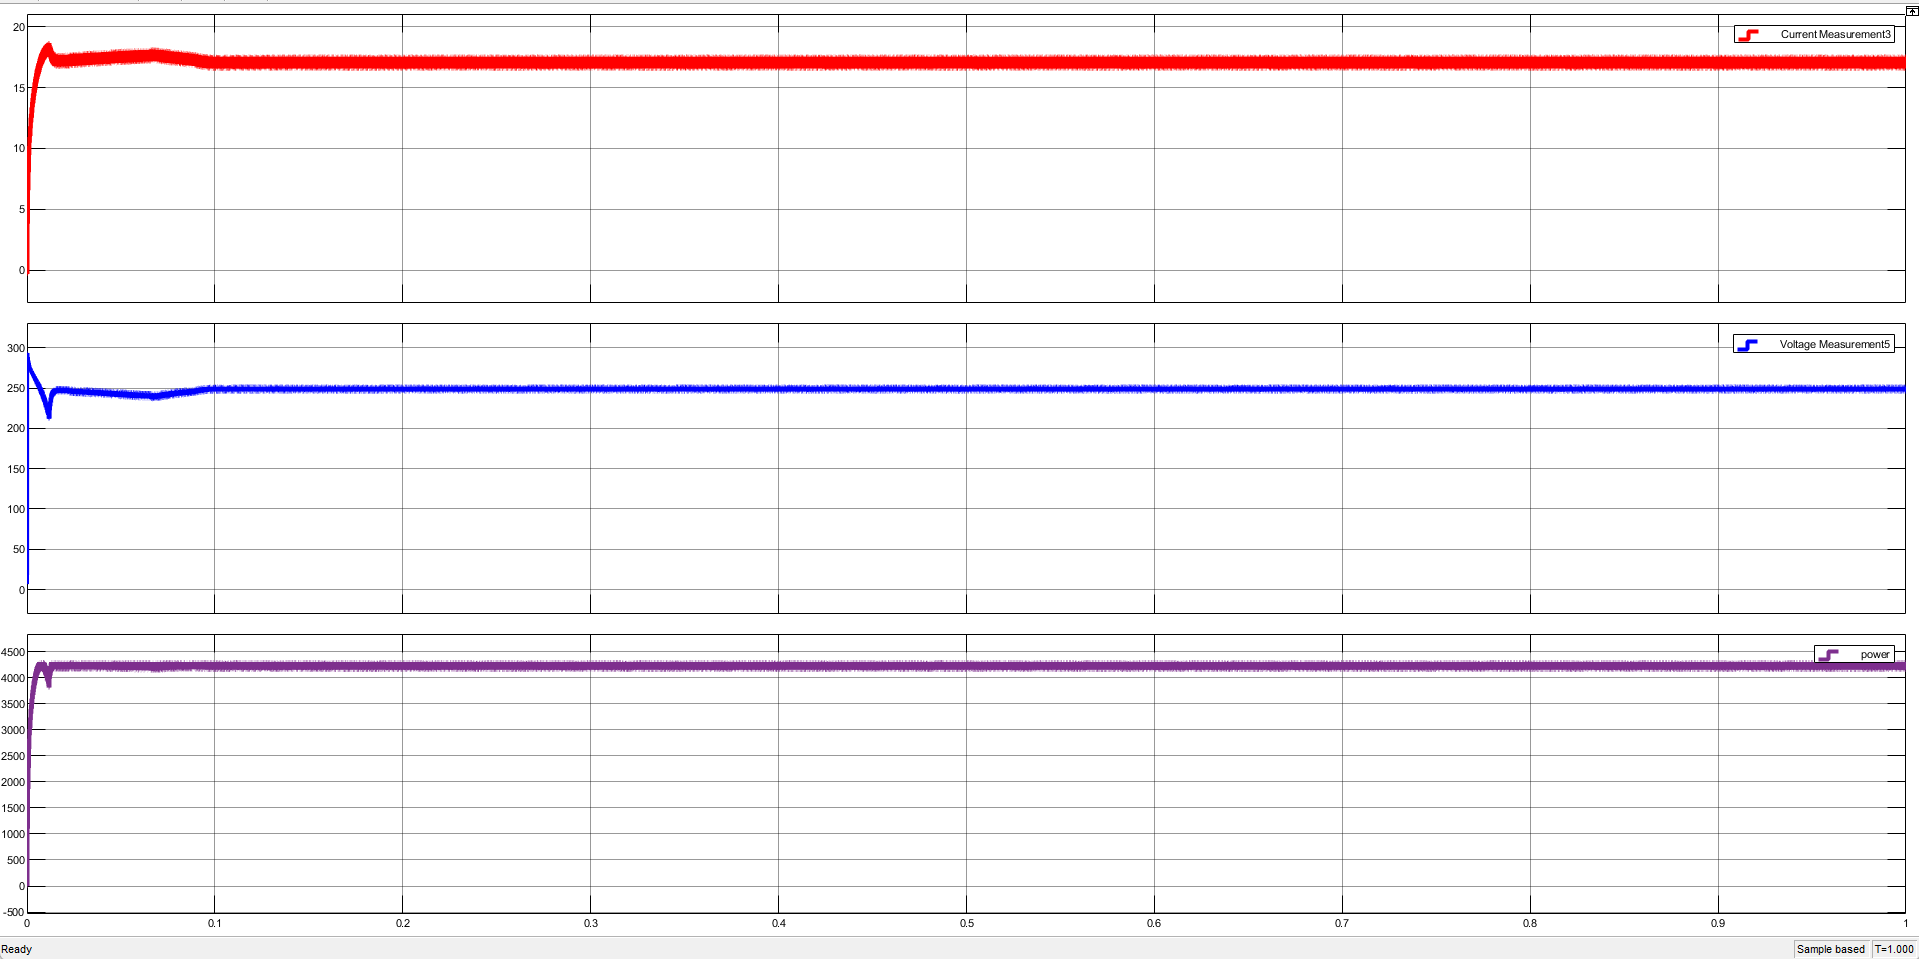
\includegraphics[width=1\textwidth]{Figures/5.1.42.png}
    \caption{Input current, voltage, power at string 1 at 250 shading.}
    \label{fig:input current, voltage, power at string 1 at 250 shading}
\end{figure}
\begin{figure}[H]
    \centering
    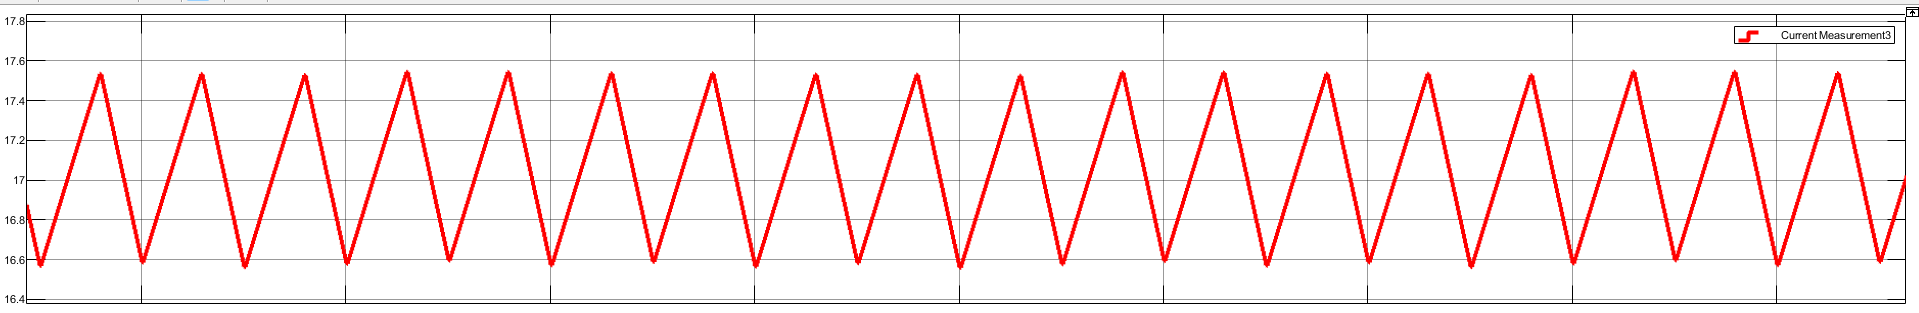
\includegraphics[width=1\textwidth]{Figures/5.1.43.png}
    \caption{Ripples of inductor current of string 1 at 250 shading.}
    \label{fig:ripples of inductor current of string 1 at 250 shading}
\end{figure}
\begin{figure}[H]
    \centering
    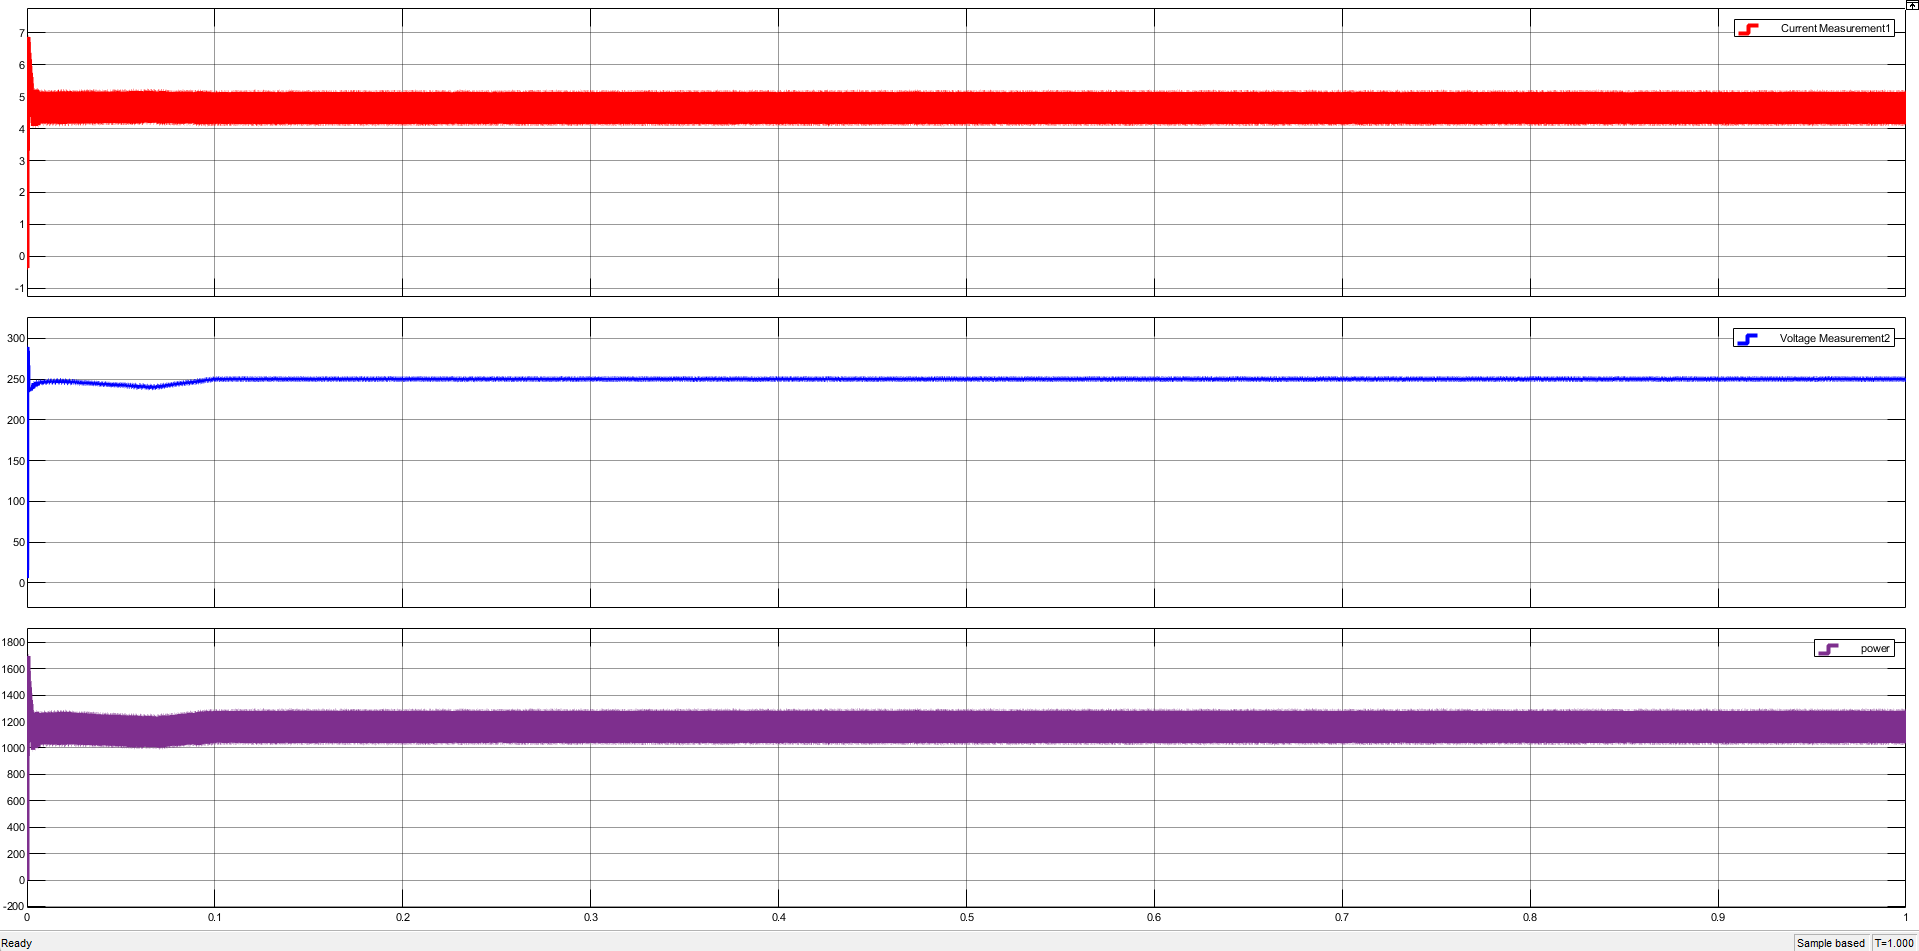
\includegraphics[width=0.9\textwidth]{Figures/5.1.44.png}
    \caption{Input current, voltage, power at string 2 at 250 shading.}
    \label{fig:input current, voltage, power at string 2 at 250 shading}
\end{figure}
\begin{figure}[H]
    \centering
    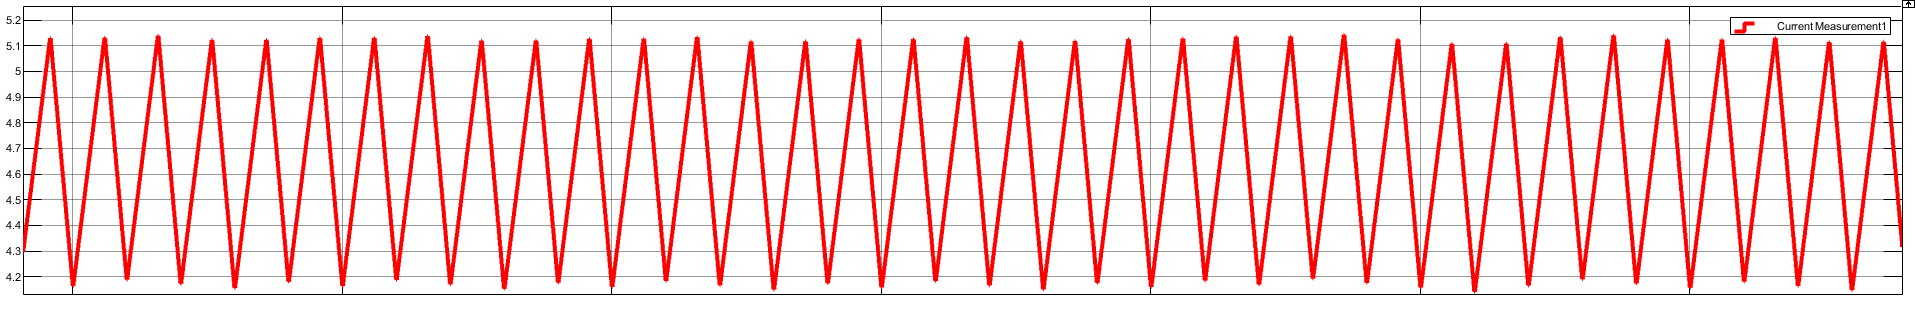
\includegraphics[width=1\textwidth]{Figures/5.1.45.png}
    \caption{Ripples of inductor current of string 2 at 250 shading.}
    \label{fig:ripples of inductor current of string 2 at 250 shading}
\end{figure}
\begin{figure}[H]
    \centering
    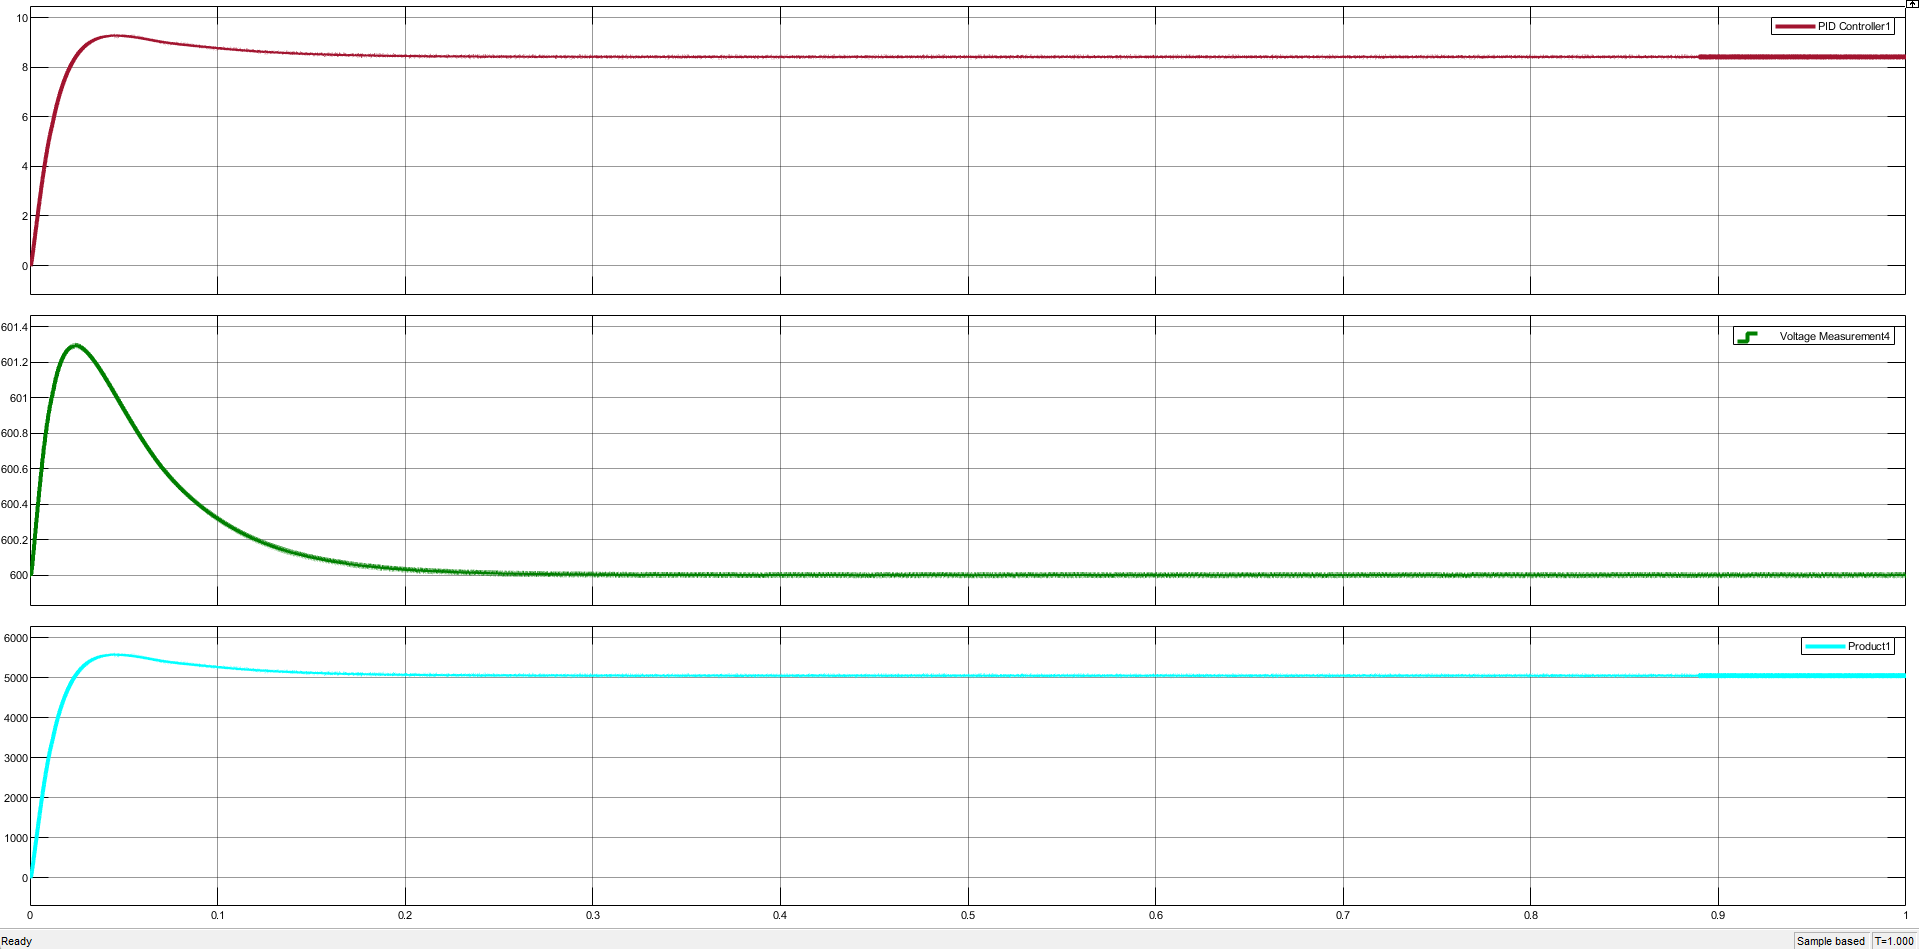
\includegraphics[width=0.9\textwidth]{Figures/5.1.46.png}
    \caption{Output current, voltage, power at 250 shading.}
    \label{fig:Output current, voltage, power at 250 shading}
\end{figure}

\subsection{Interleaved Central Configuration}
\subsubsection{Topology of Interleaved Boost Converter}
% ==========================================================
% SECTION 5.1.4: TWO-PHASE INTERLEAVED BOOST CONVERTER DESIGN
% ==========================================================

Conventional boost converters exhibit inherent performance limitations when deployed in high-power applications, primarily characterized by elevated input current ripple and increased thermal stress on switching devices. To mitigate these drawbacks and ensure optimal power extraction from the $8520\text{ W}$ photovoltaic (PV) array, a Two-Phase Interleaved Boost Converter (IBC) architecture was selected.

While a standard single-phase boost converter offers a lower component count, the interleaved configuration provides critical operational advantages for high-power integration across three primary domains:

\begin{enumerate}
    \item \textbf{Interleaving and Ripple Cancellation:} \\
    By implementing a $180^\circ$ spatial phase shift between the gate-drive control signals of the two parallel switching branches, the high-frequency inductor current ripples actively undergo destructive interference (cancellation). This interleaving mechanism yields a significantly smoother net input current waveform. Minimizing this current ripple prevents high-frequency voltage oscillations at the PV terminals, thereby enhancing the tracking precision and dynamic stability of the Global Maximum Power Point Tracking (GMPPT) algorithm.
    \newpage
    \item \textbf{Thermal Distribution via Current Sharing:} \\
    Under nominal peak operating conditions, the total array output current of $34.72\text{ A}$ is uniformly split between the two interleaved channels. Consequently, each discrete phase conducts an average current of only $17.36\text{ A}$. This reduction in localized current density scales down conduction losses ($I^2R$) and switching stresses across the power MOSFETs and diodes, minimizing thermal dissipation, improving reliability, and boosting the converter's net conversion efficiency.   
    \item \textbf{Volumetric and Filter Optimization:} \\
    The multi-phase interleaved operation effectively doubles the fundamental ripple frequency seen at the input and output filter stages ($f_{\text{ripple}} = 2f_s$). Because the required filter inductance and capacitance values are inversely proportional to the operating ripple frequency, this frequency doubling dramatically reduces the structural requirements for the passive components. As a result, the physical size, weight, magnetic core volume, and overall manufacturing cost of the power electronic interface are significantly minimized.
\end{enumerate}

\begin{figure}[H]
    \centering
    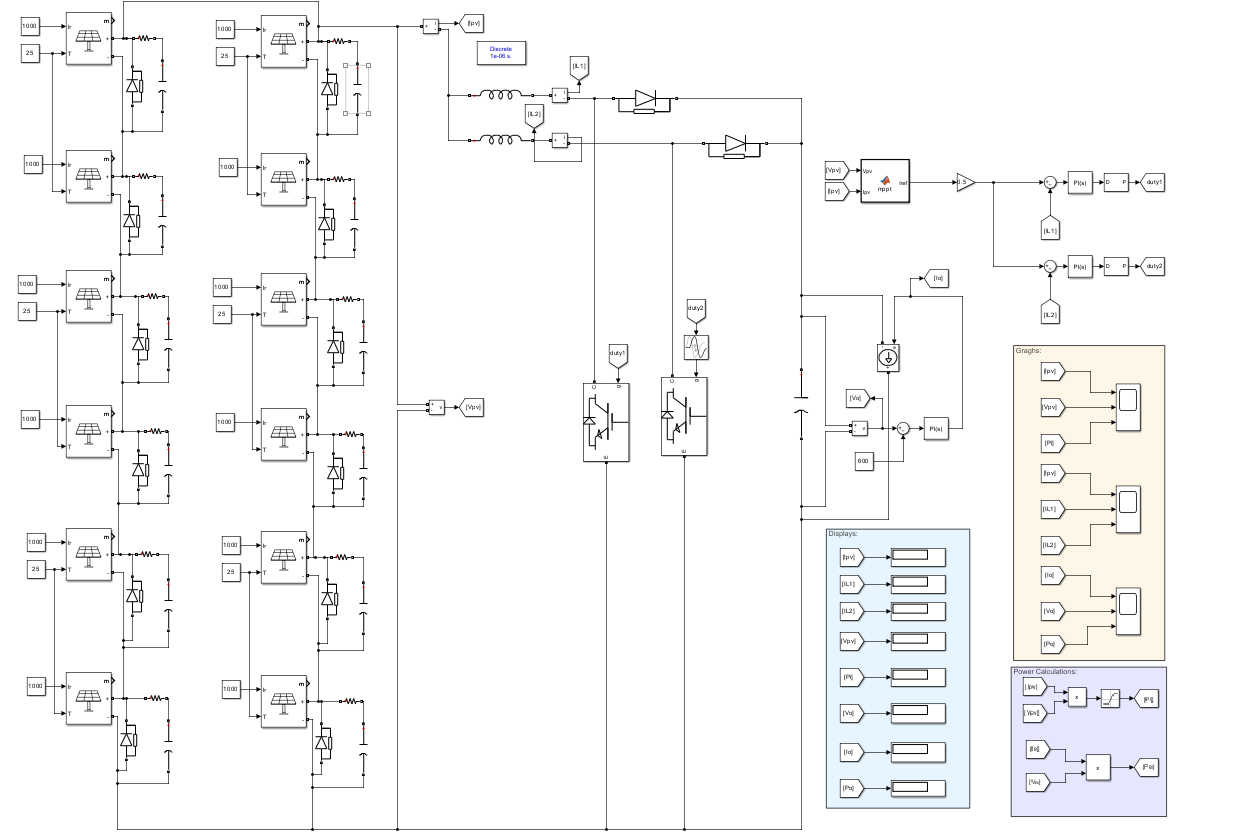
\includegraphics[width=1.1\textwidth]{Figures/5.1.47.png}
    \caption{ Interleaved central with load configuration.}
    \label{fig:interleaved central with load configuration}
\end{figure}

\subsubsection{Results of Simulation in Case of No Shading}
\noindent
\begin{minipage}[t]{0.5\textwidth}
\vspace{0pt}
\begin{itemize}
  \item The power display shows 8490\,W, which is nearly identical to the theoretical 8520\,W target. This confirms that the code is accurately tracking the Maximum Power Point.
  \item \textbf{DC-Link Stability:} The output voltage ($V_{DC}$) is maintained at
        exactly 600\,V. This proves that the DC-Link Voltage Control loop
        ($K_p = 8$, $K_i = 80$) and the Bulk Capacitor are effectively regulating the
        output despite the high-power flow.
   \item \textbf{Current sharing:} the inductor currents are almost equal and the input values of voltage and current align with the design calculation.      
  \item Ripples of inductor current $= 35.2 - 34.9 = 0.3$\,A.as seen ripples of current significantly decreases. 
\end{itemize}
\end{minipage}
\hfill
\begin{minipage}[t]{0.4\textwidth}
\vspace{0pt}
  \centering
  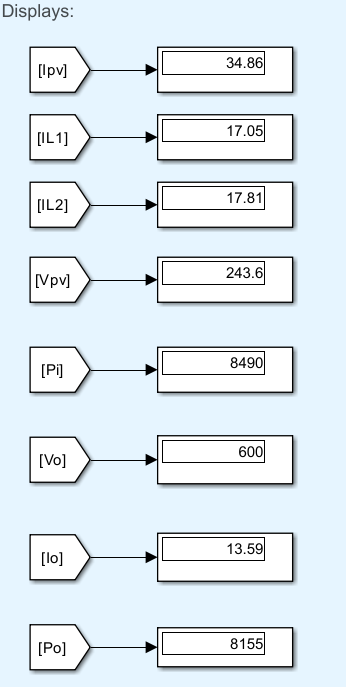
\includegraphics[width=\textwidth]{Figures/5.1.48.png}
  \captionof{figure}{Displays of interleaved central configuration.}
  \label{fig:displays of interleaved central configuration.}
\end{minipage}
\paragraph{Graphs}
\begin{figure}[H]
    \centering
    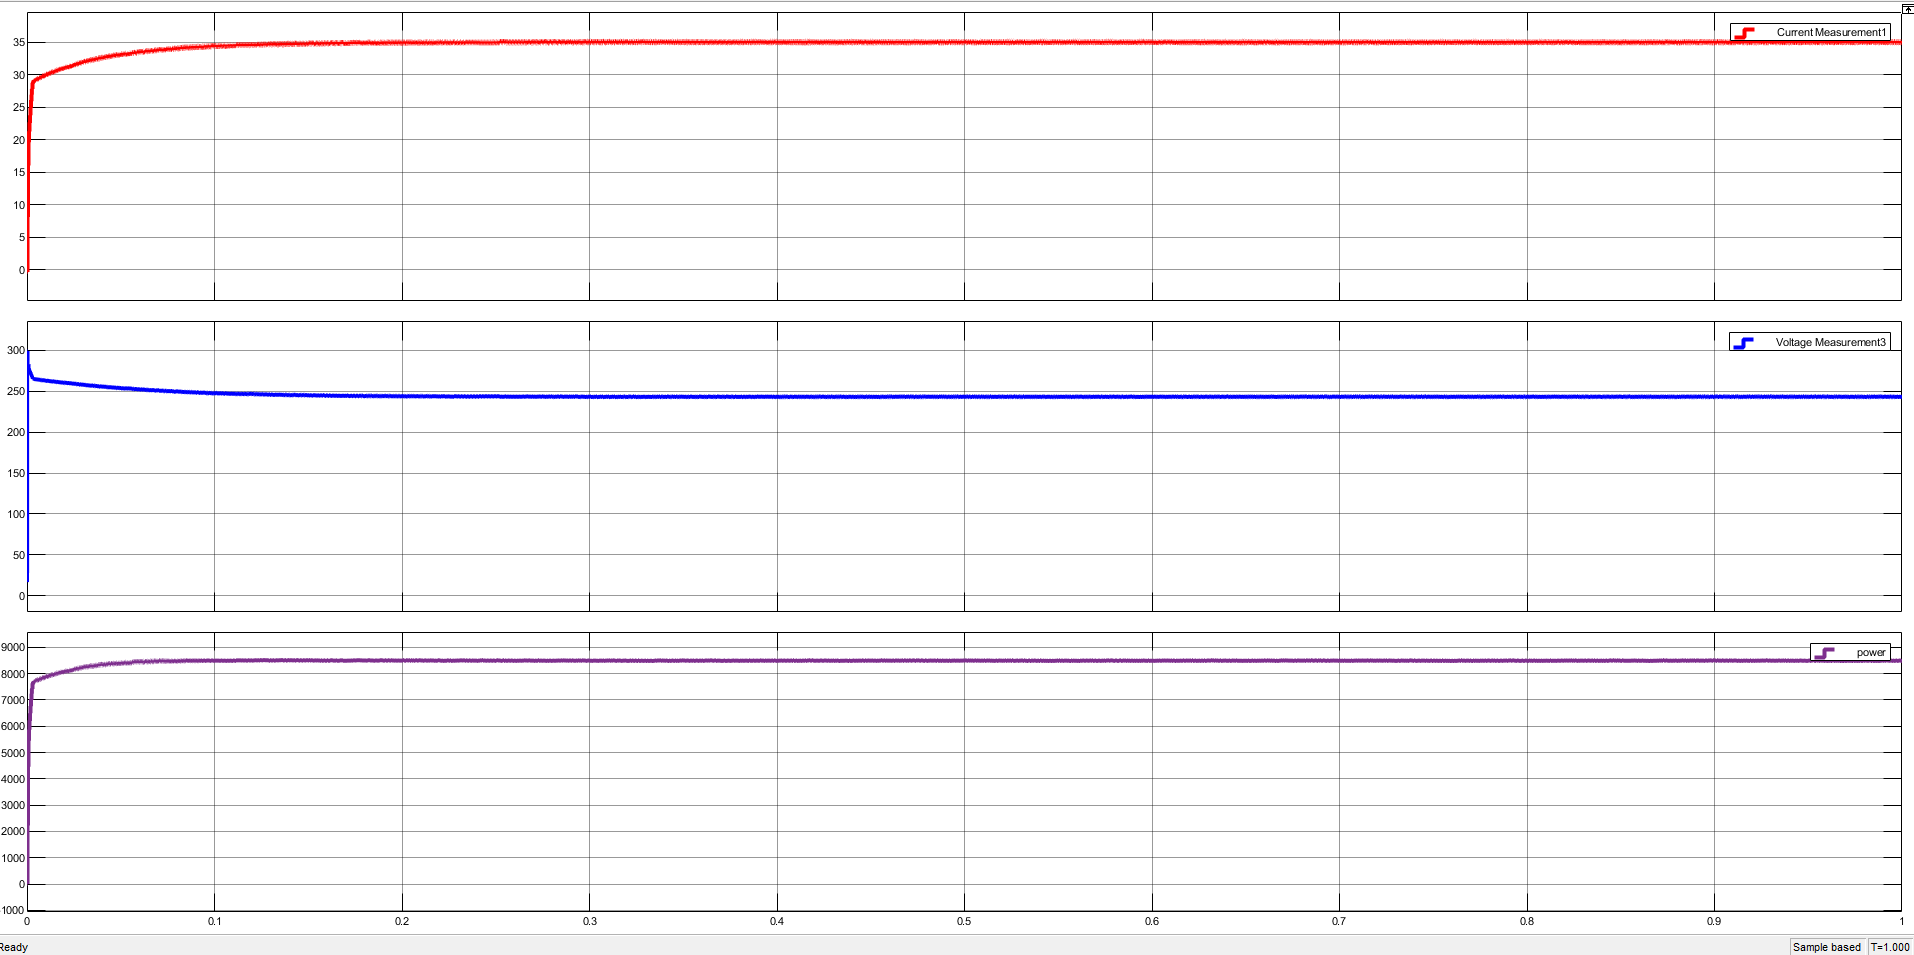
\includegraphics[width=0.9\textwidth]{Figures/5.1.49.png}
    \caption{Input current, voltage, power of interleaved central.}
    \label{fig:input current, voltage, power at no shading at interleaved central}
\end{figure}
\begin{figure}[H]
    \centering
    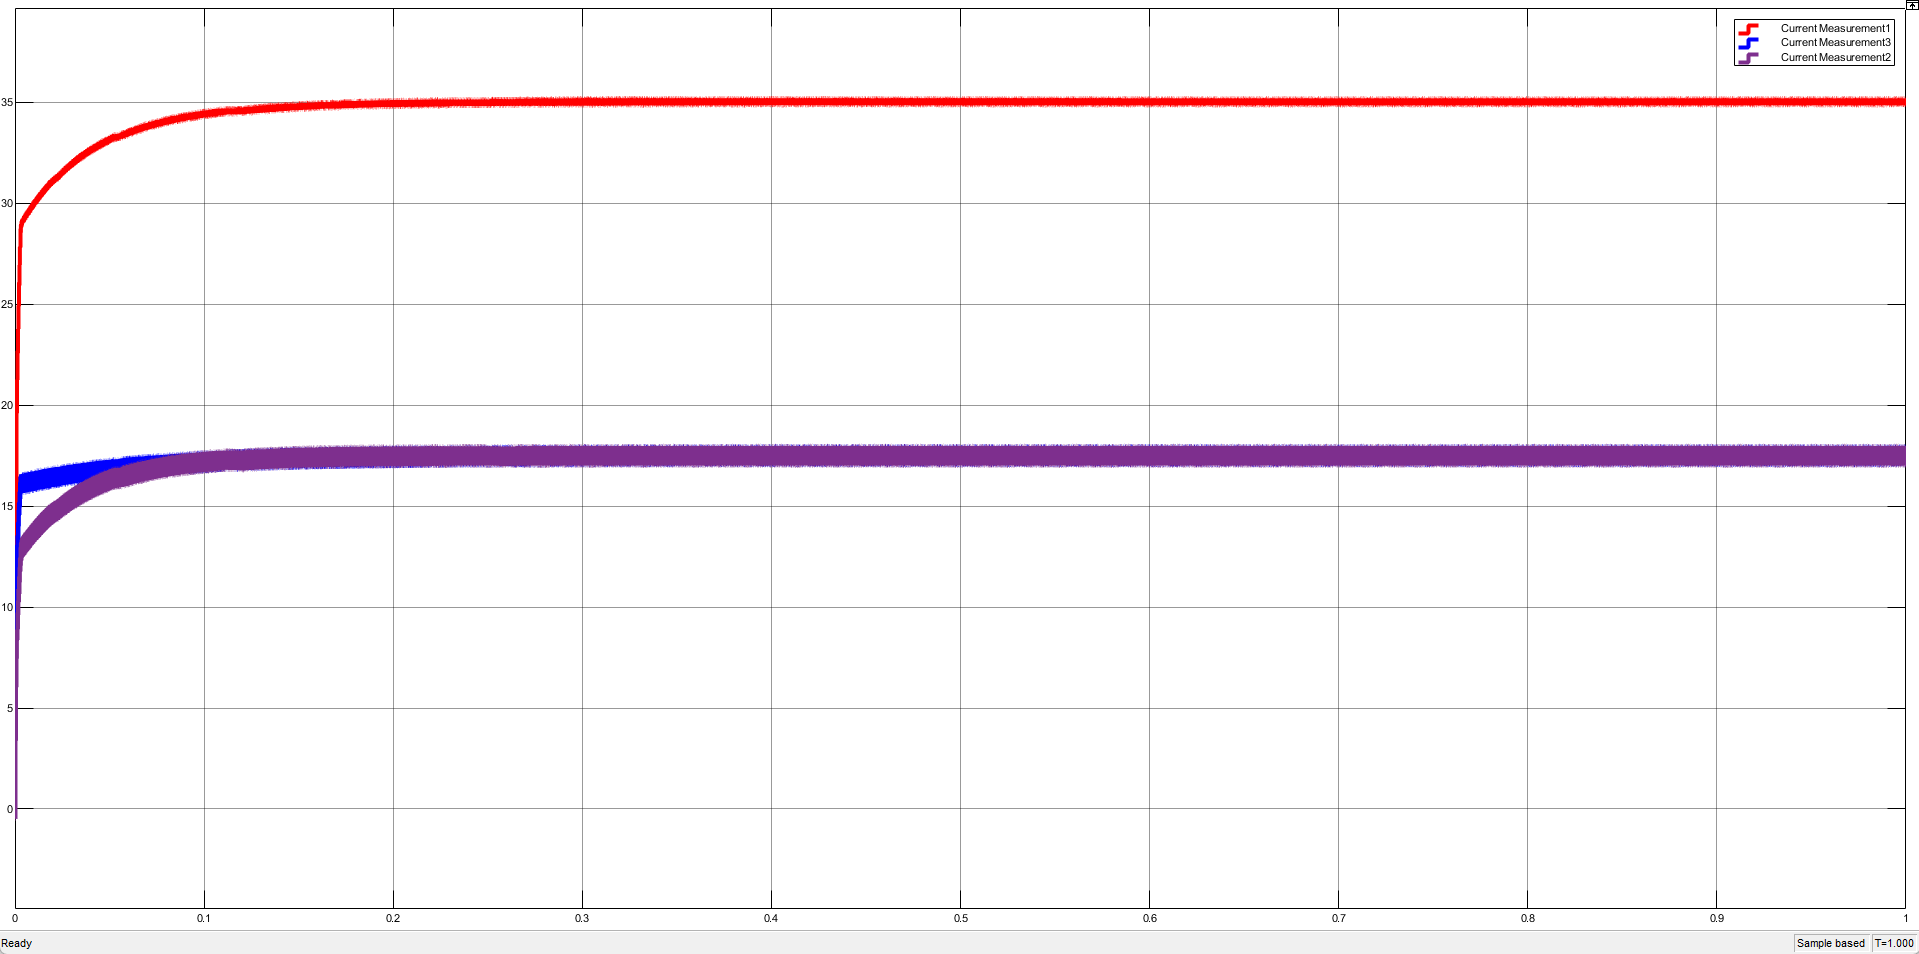
\includegraphics[width=0.9\textwidth]{Figures/5.1.50.png}
    \caption{Input total current, inductor current 1, inductor current 2.}
    \label{fig:input total current, inductor current 1, inductor current 2 at no shading at interleaved central}
\end{figure}
\begin{figure}[H]
    \centering
    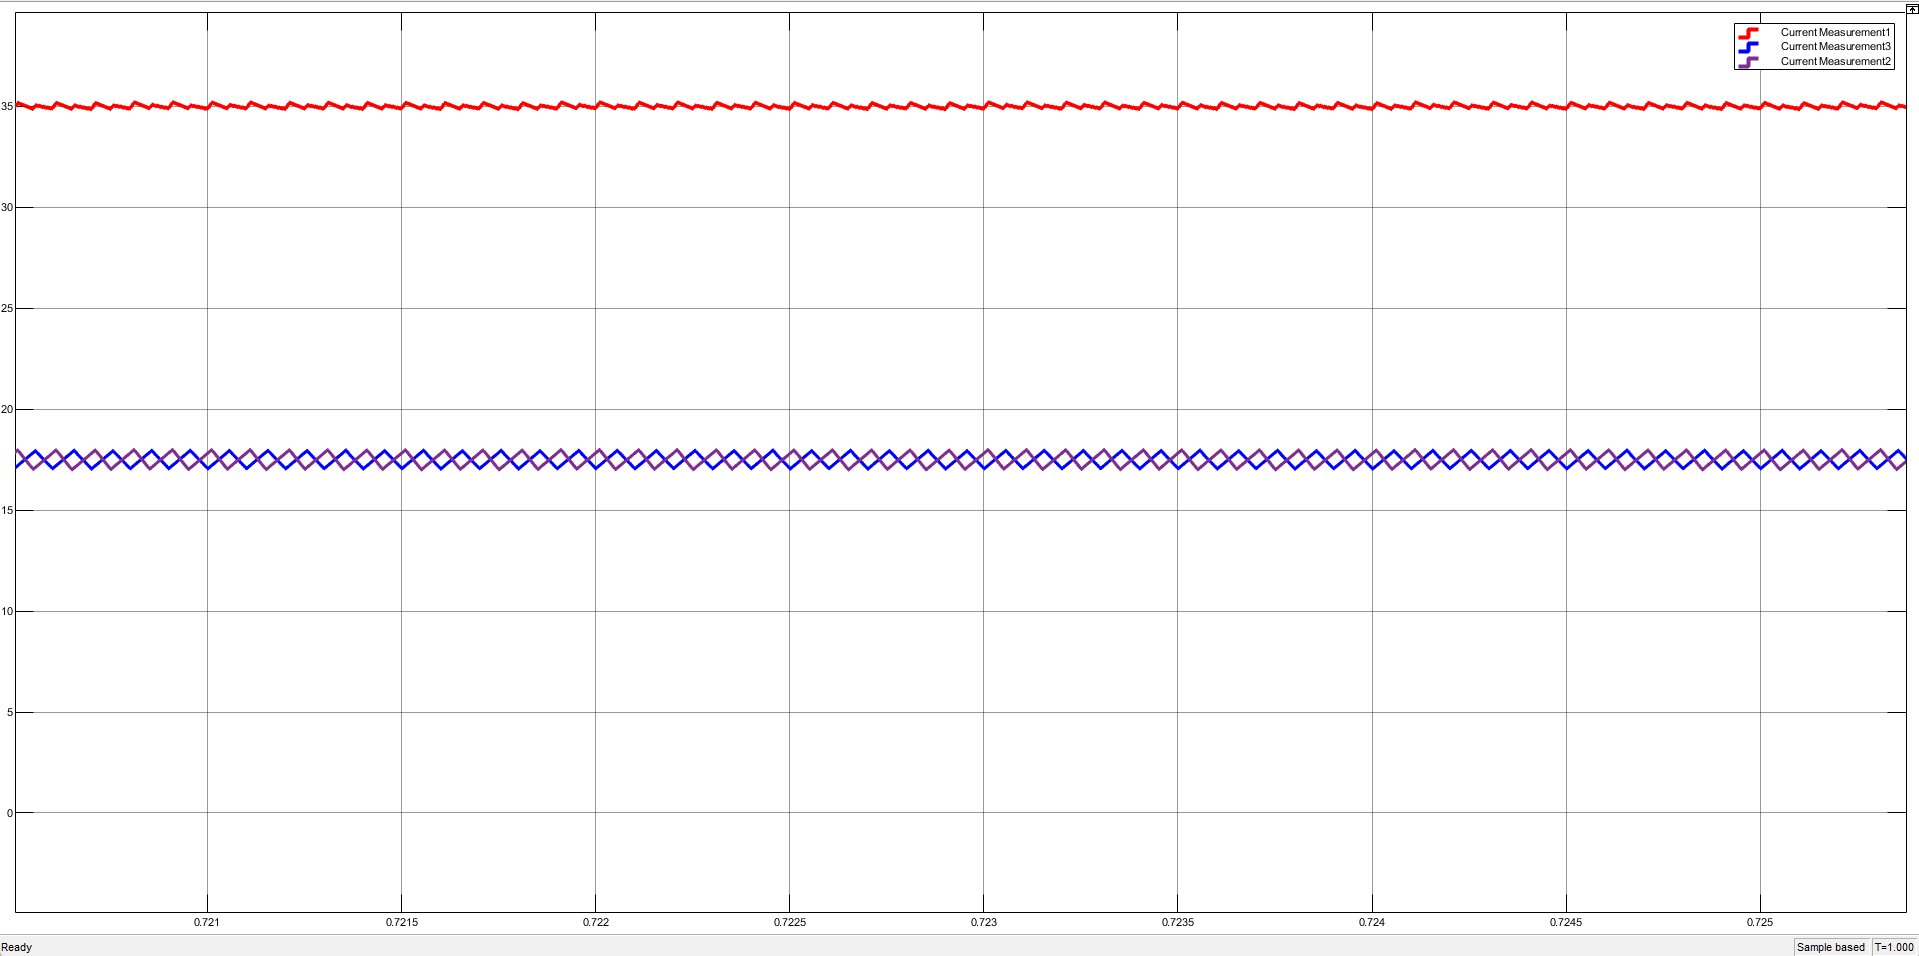
\includegraphics[width=0.9\textwidth]{Figures/5.1.51.png}
    \caption{Input total current, inductor current 1, inductor current 2.}
    \label{fig:input total current, inductor current 1, inductor current 2 zoom at no shading at interleaved central}
\end{figure}
\begin{figure}[H]
    \centering
    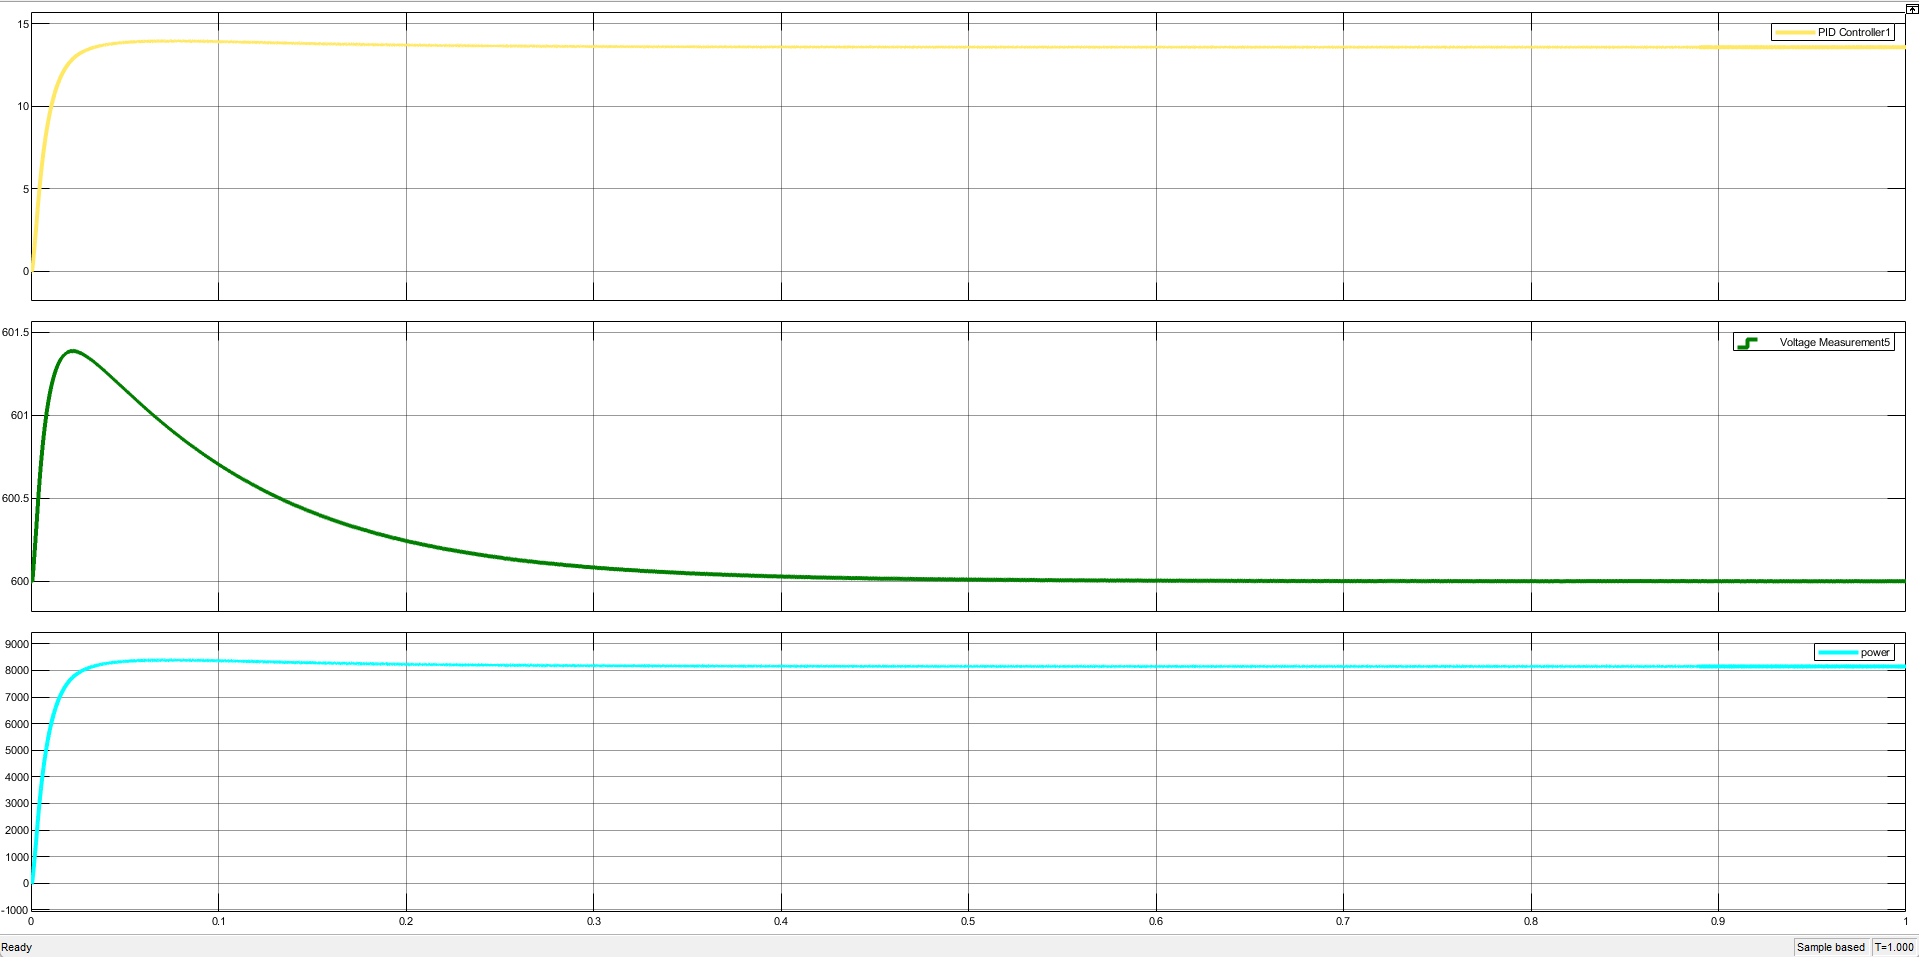
\includegraphics[width=0.9\textwidth]{Figures/5.1.52.png}
    \caption{Output current, voltage, power of interleaved central.}
    \label{fig:output current, voltage, power at no shading at interleaved central}
\end{figure}


\subsection{String Interleaved Configuration}
\begin{figure}[H]
    \centering
    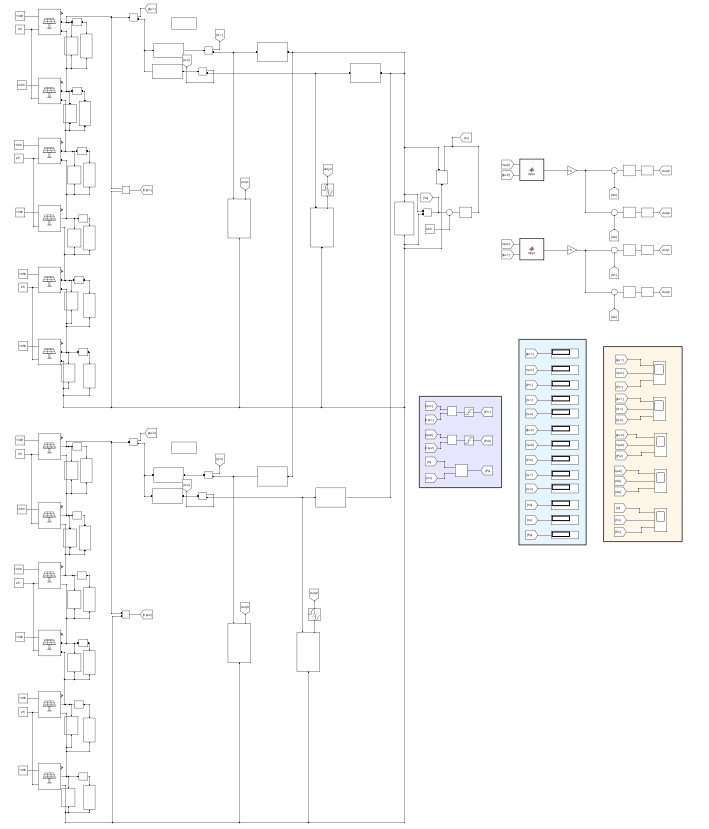
\includegraphics[width=1\textwidth]{Figures/5.1.53.png}
    \caption{ Interleaved string with load configuration.}
    \label{fig:interleaved string with load configuration}
\end{figure}
\subsubsection{Results of Simulation in Case of No Shading}
\noindent
\begin{minipage}[t]{0.5\textwidth}
\vspace{0pt}
\begin{itemize}
  \item Each string has its own interleaved boost converter with common dc link, so each string has its own MPPT and both tracks correctly max power.
  \item \textbf DC-Link  is maintained at exactly 600\,V due to PI closed loop control ($K_p = 5$, $K_i = 150$)
   \item \textbf{Current sharing:} the inductor currents are almost equal and the input values of voltage and current align with the design calculation.      
  \item Ripples of total inductor current of string 1 $= 35.2 - 34.9 = 0.3$\,A.as seen ripples of current significantly decreases. 
  \item Ripples of total inductor current of string 1 $= 35.2 - 34.9 = 0.3$\,A.as seen ripples of current significantly decreases.
\end{itemize}
\end{minipage}
\hfill
\begin{minipage}[t]{0.4\textwidth}
\vspace{0pt}
  \centering
  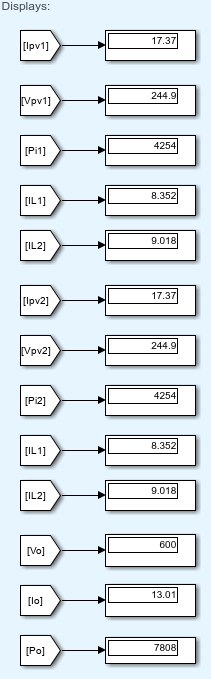
\includegraphics[width=\textwidth]{Figures/5.1.54.png}
  \captionof{figure}{Displays of interleaved string configuration..}
  \label{fig:Displays of interleaved string configuration.}
\end{minipage}

\begin{figure}[H]
    \centering
    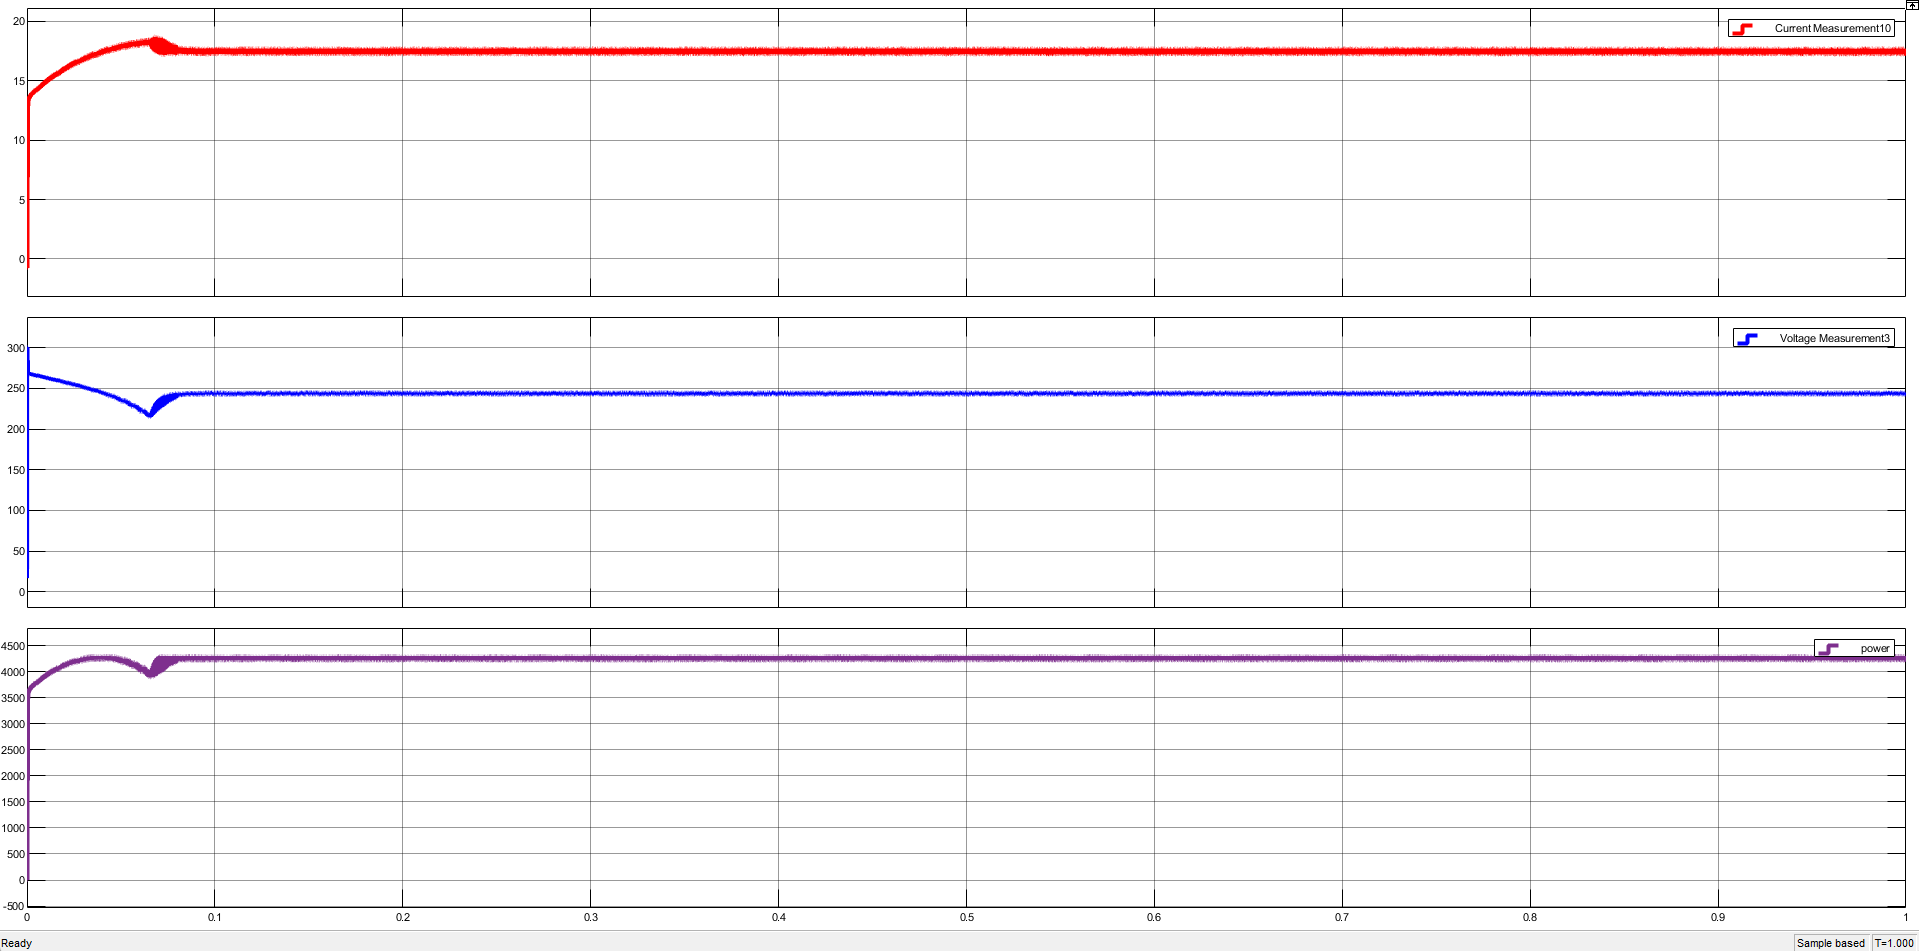
\includegraphics[width=0.9\textwidth]{Figures/5.1.55.png}
    \caption{Input current, voltage, power at string 1 of interleaved string.}
    \label{fig:input current, voltage, power at no shading at interleaved string at string 1}
\end{figure}
\begin{figure}[H]
    \centering
    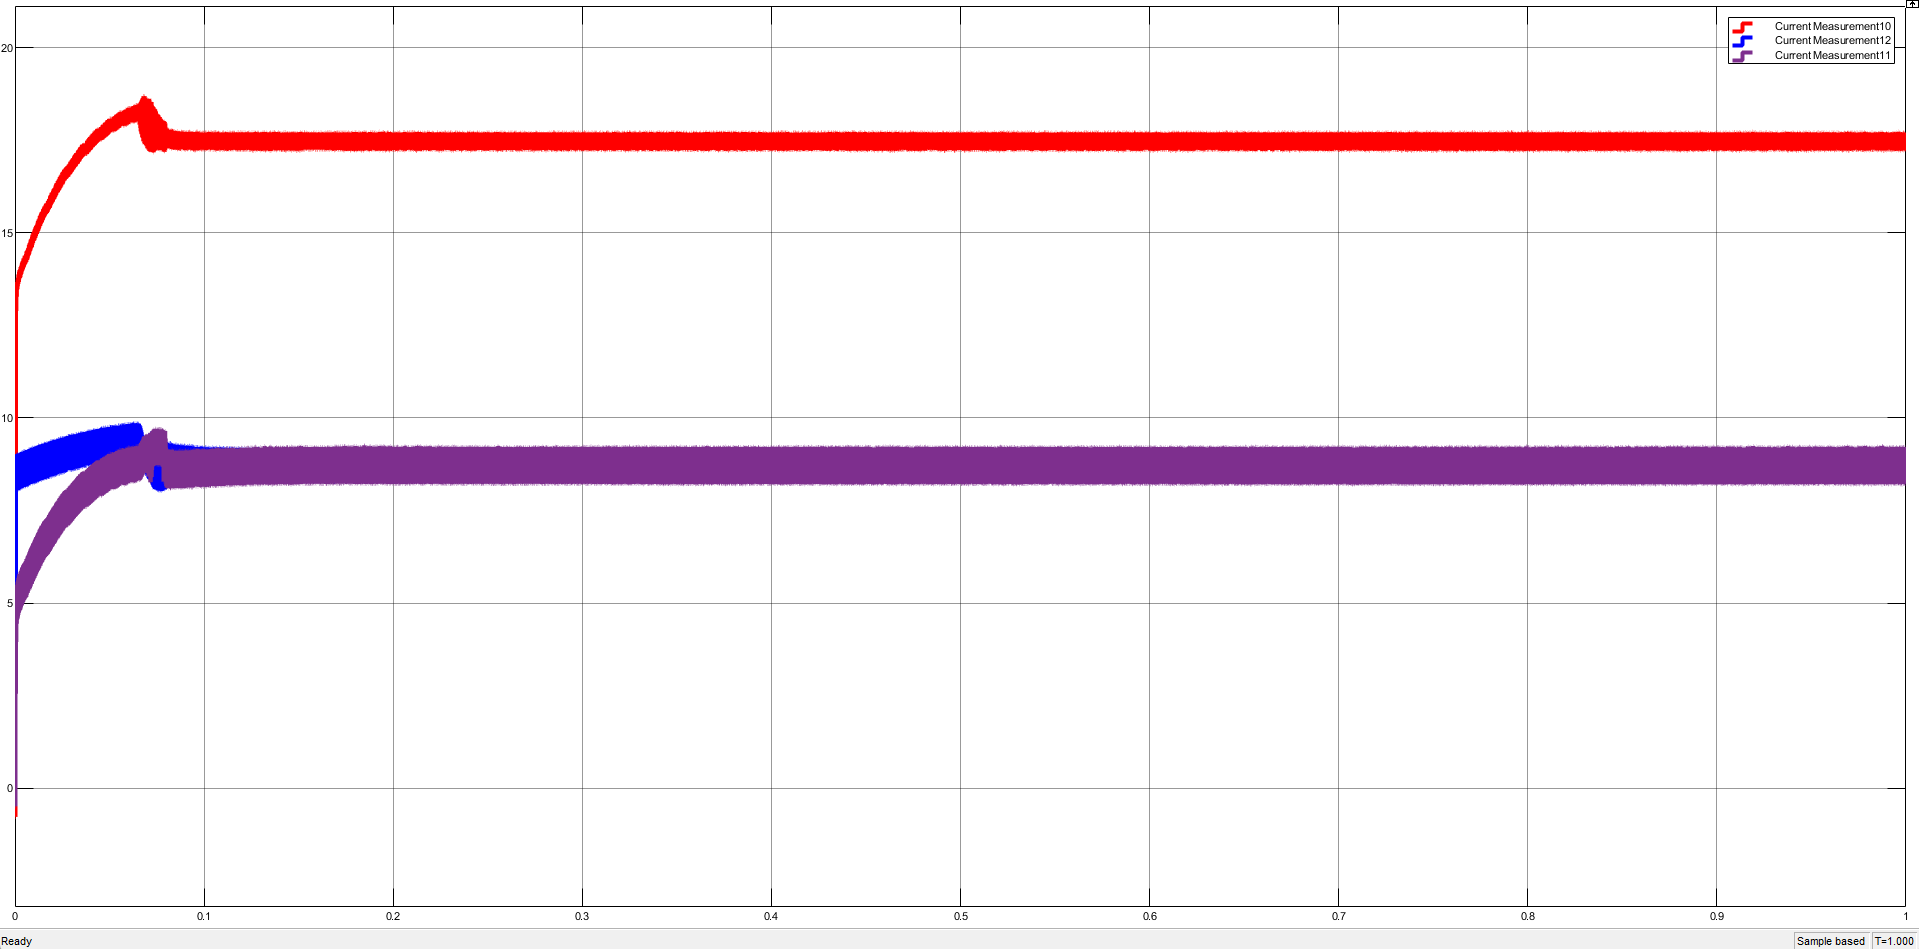
\includegraphics[width=0.9\textwidth]{Figures/5.1.56.png}
    \caption{Input total current, inductor current 1, inductor current 2 at string 1.}
    \label{fig:input total current, inductor current 1, inductor current 2 at no shading at interleaved string at string 1}
\end{figure}
\begin{figure}[H]
    \centering
    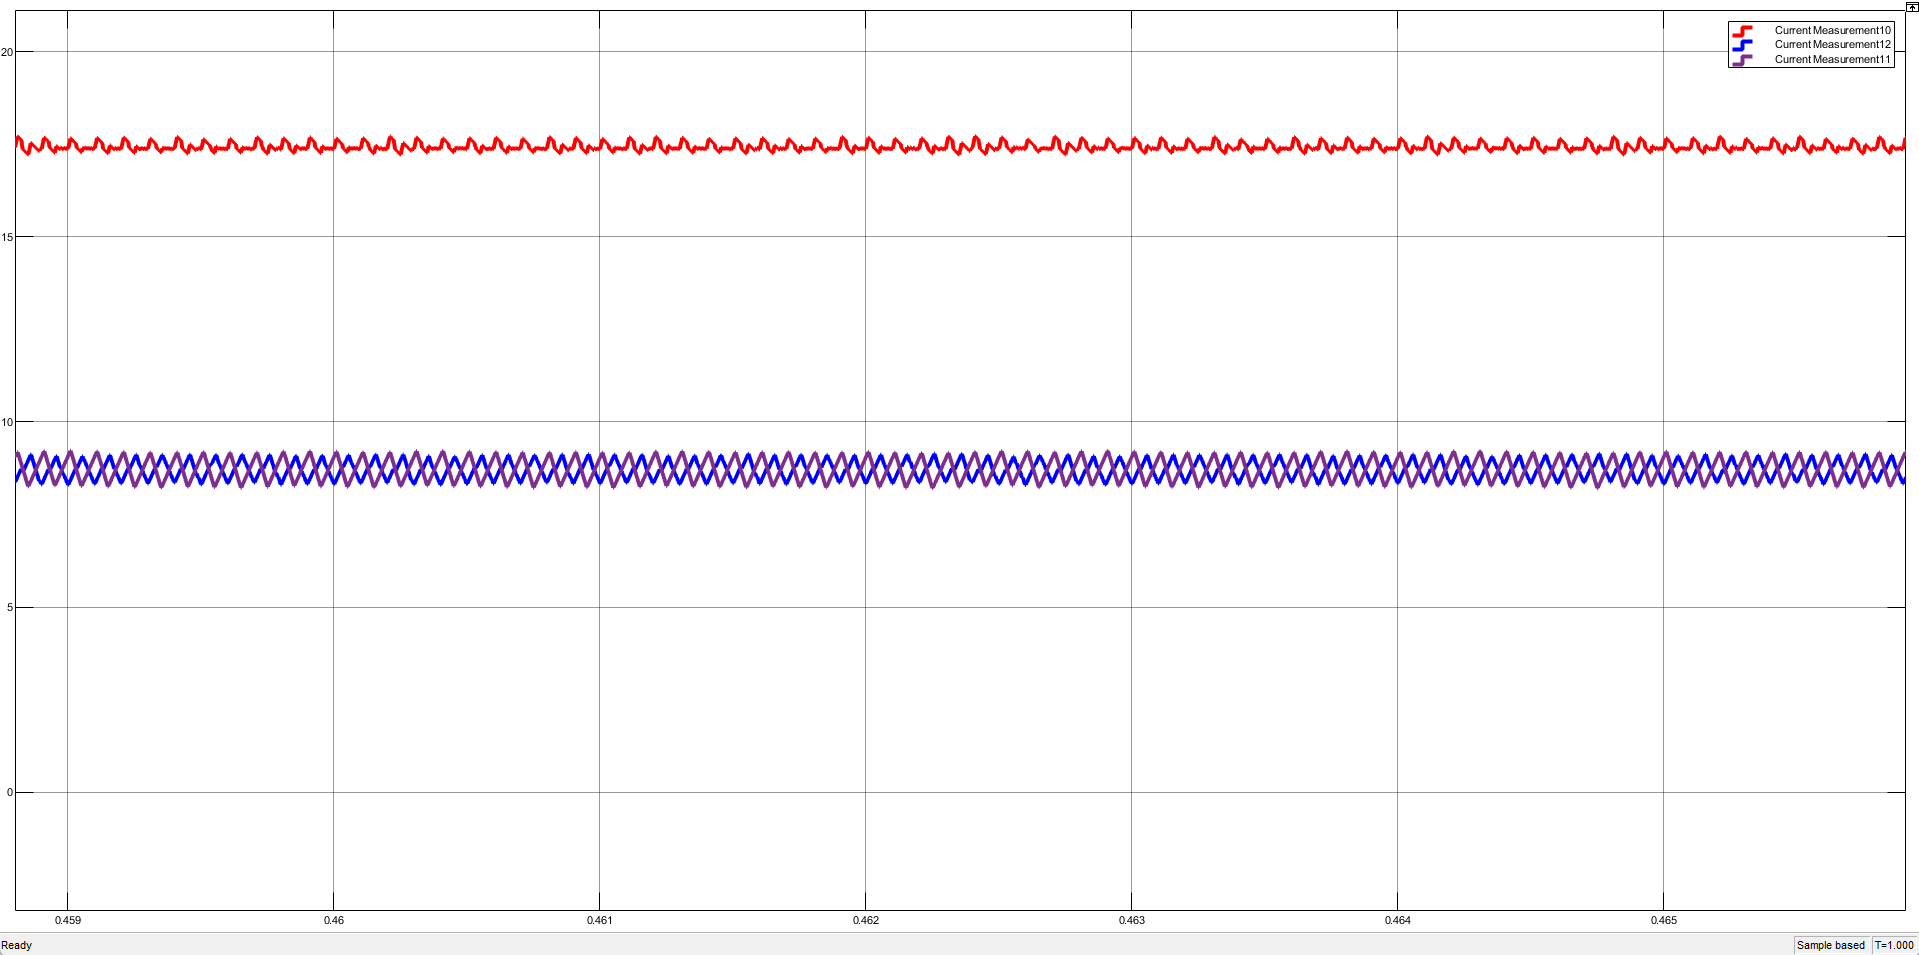
\includegraphics[width=0.9\textwidth]{Figures/5.1.57.png}
    \caption{Input total current, inductor current 1, inductor current 2 at string 1.}
    \label{fig:input total current, inductor current 1, inductor current 2 zoom at no shading at interleaved string at string 1}
\end{figure}
\begin{figure}[H]
    \centering
    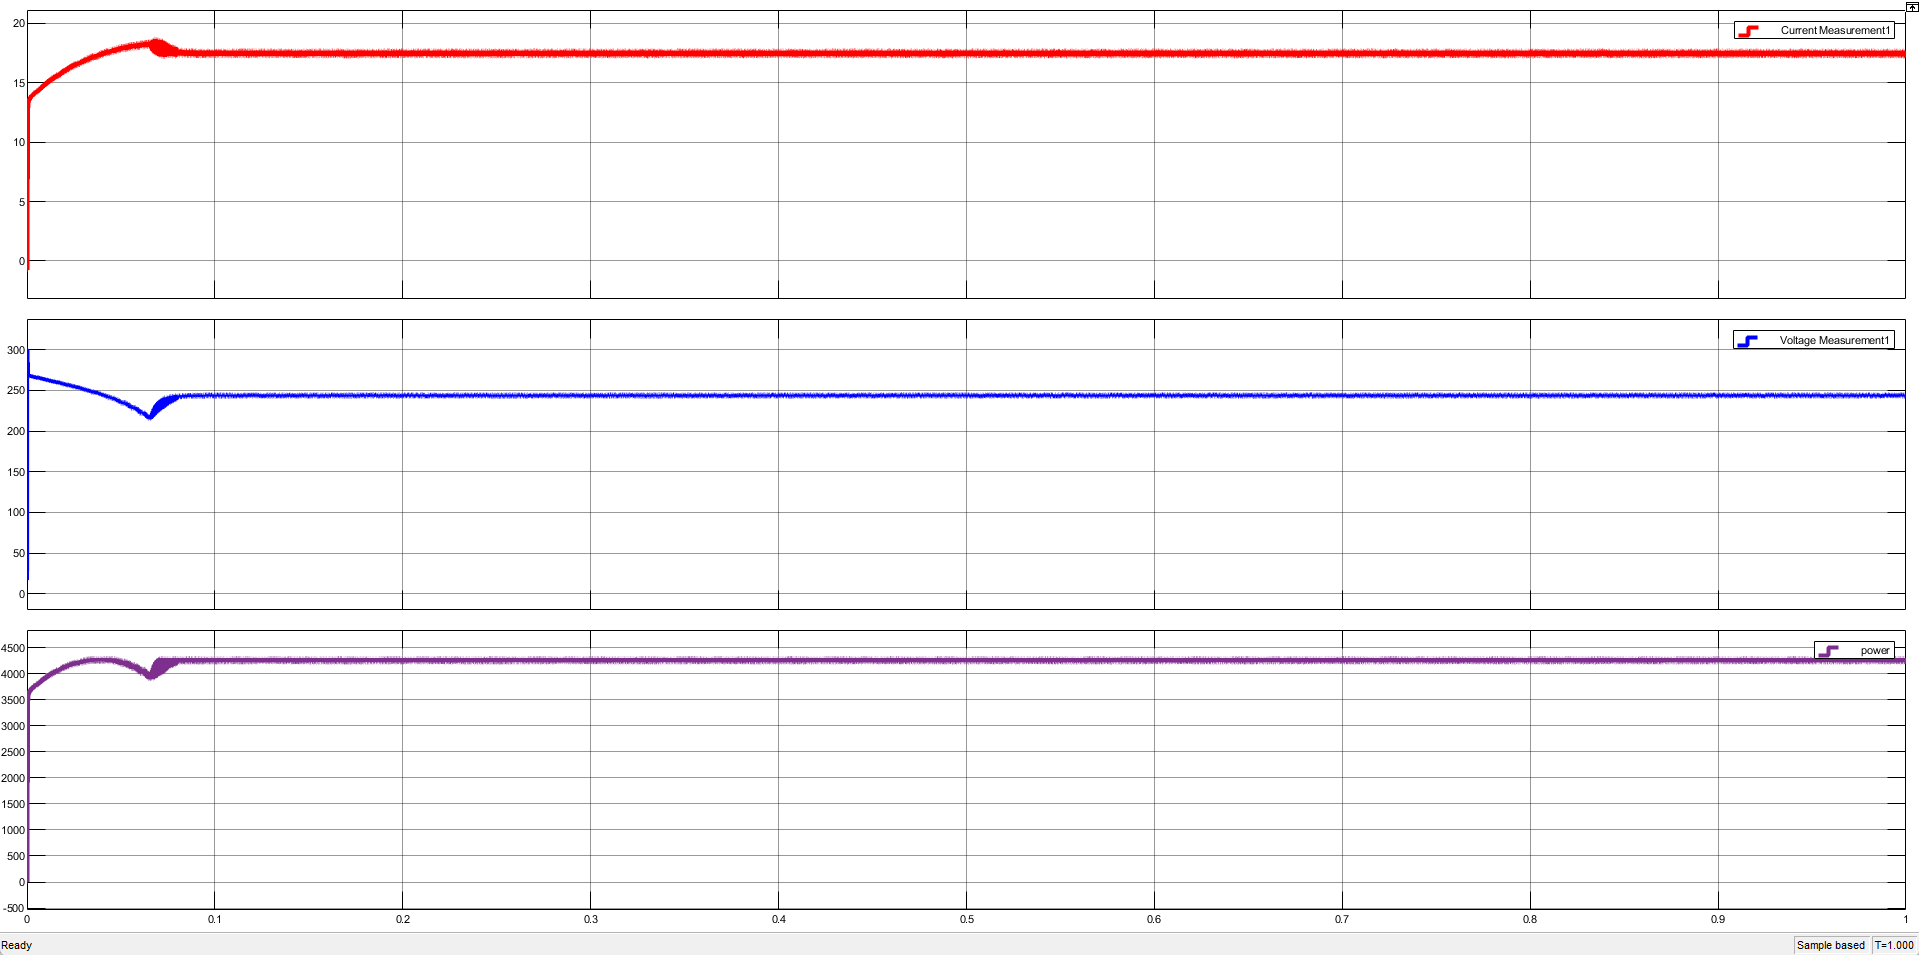
\includegraphics[width=0.9\textwidth]{Figures/5.1.58.png}
    \caption{Input current, voltage, power at string 2 of interleaved string.}
    \label{fig:input current, voltage, power at no shading at interleaved string at string 2}
\end{figure}
\begin{figure}[H]
    \centering
    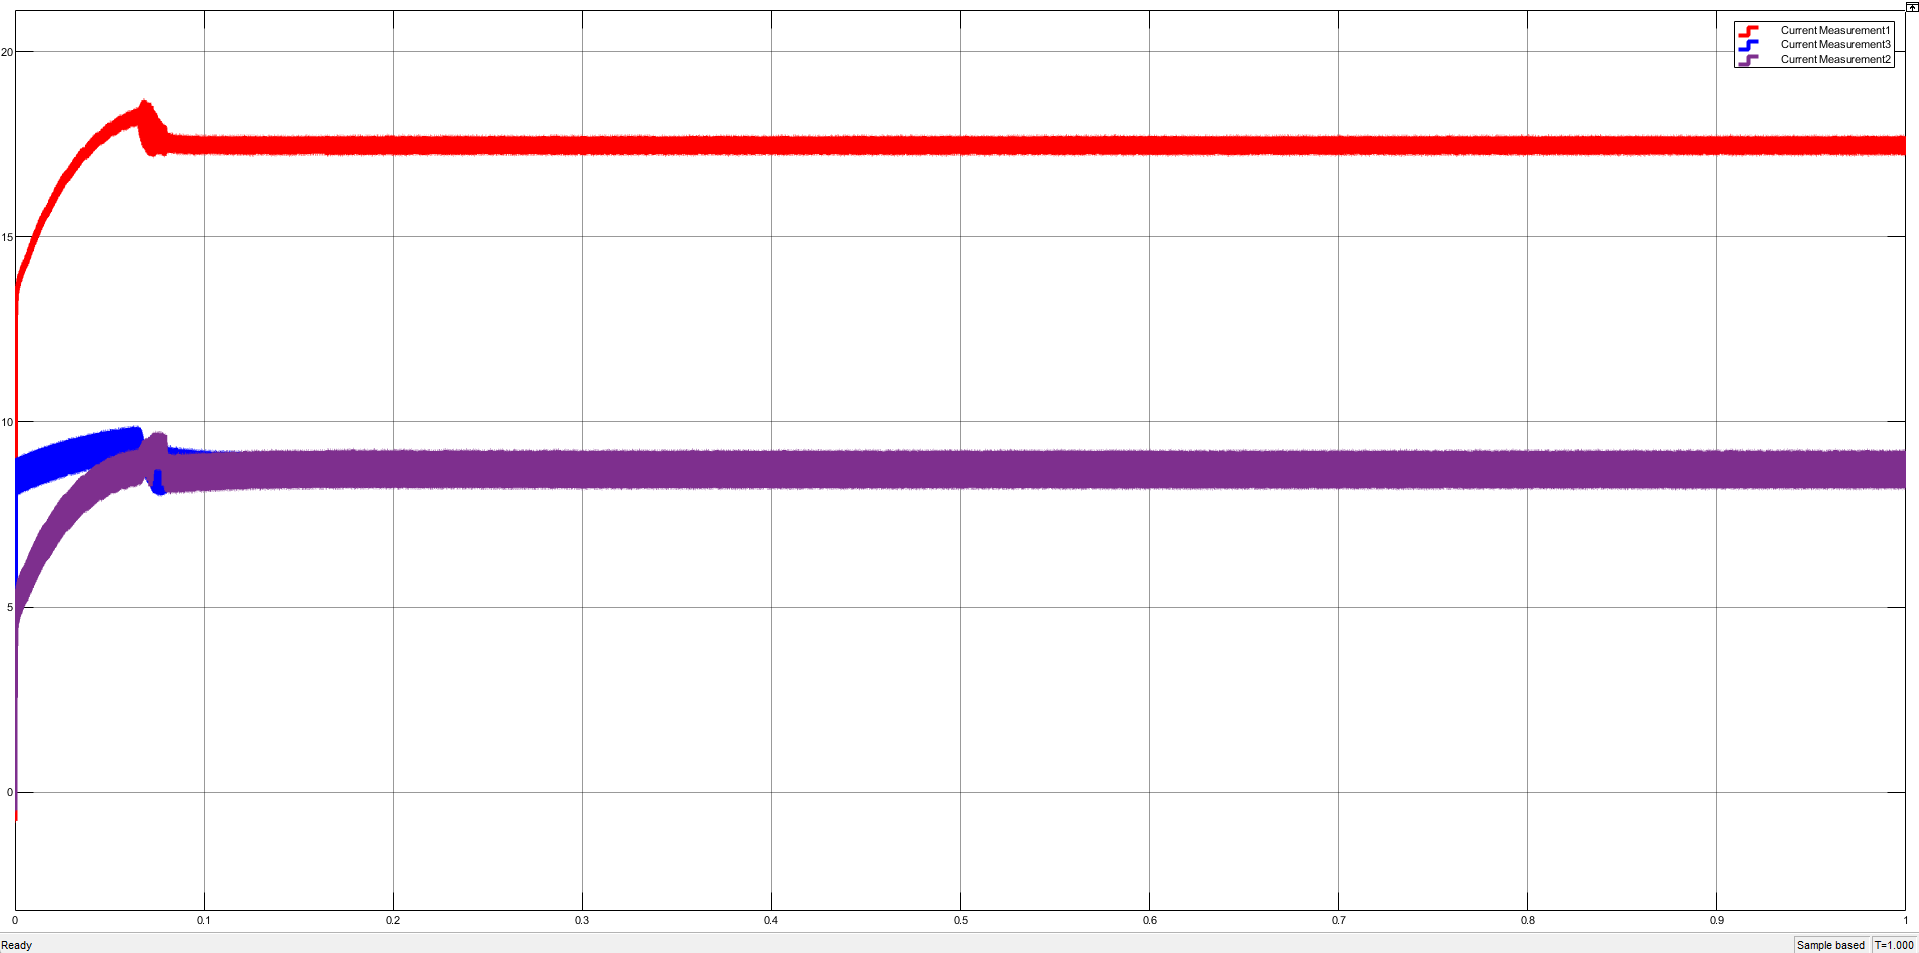
\includegraphics[width=0.9\textwidth]{Figures/5.1.59.png}
    \caption{Input total current, inductor current 1, inductor current 2 at string 2.}
    \label{fig:input total current, inductor current 1, inductor current 2 at no shading at interleaved string at string 2}
\end{figure}
\begin{figure}[H]
    \centering
    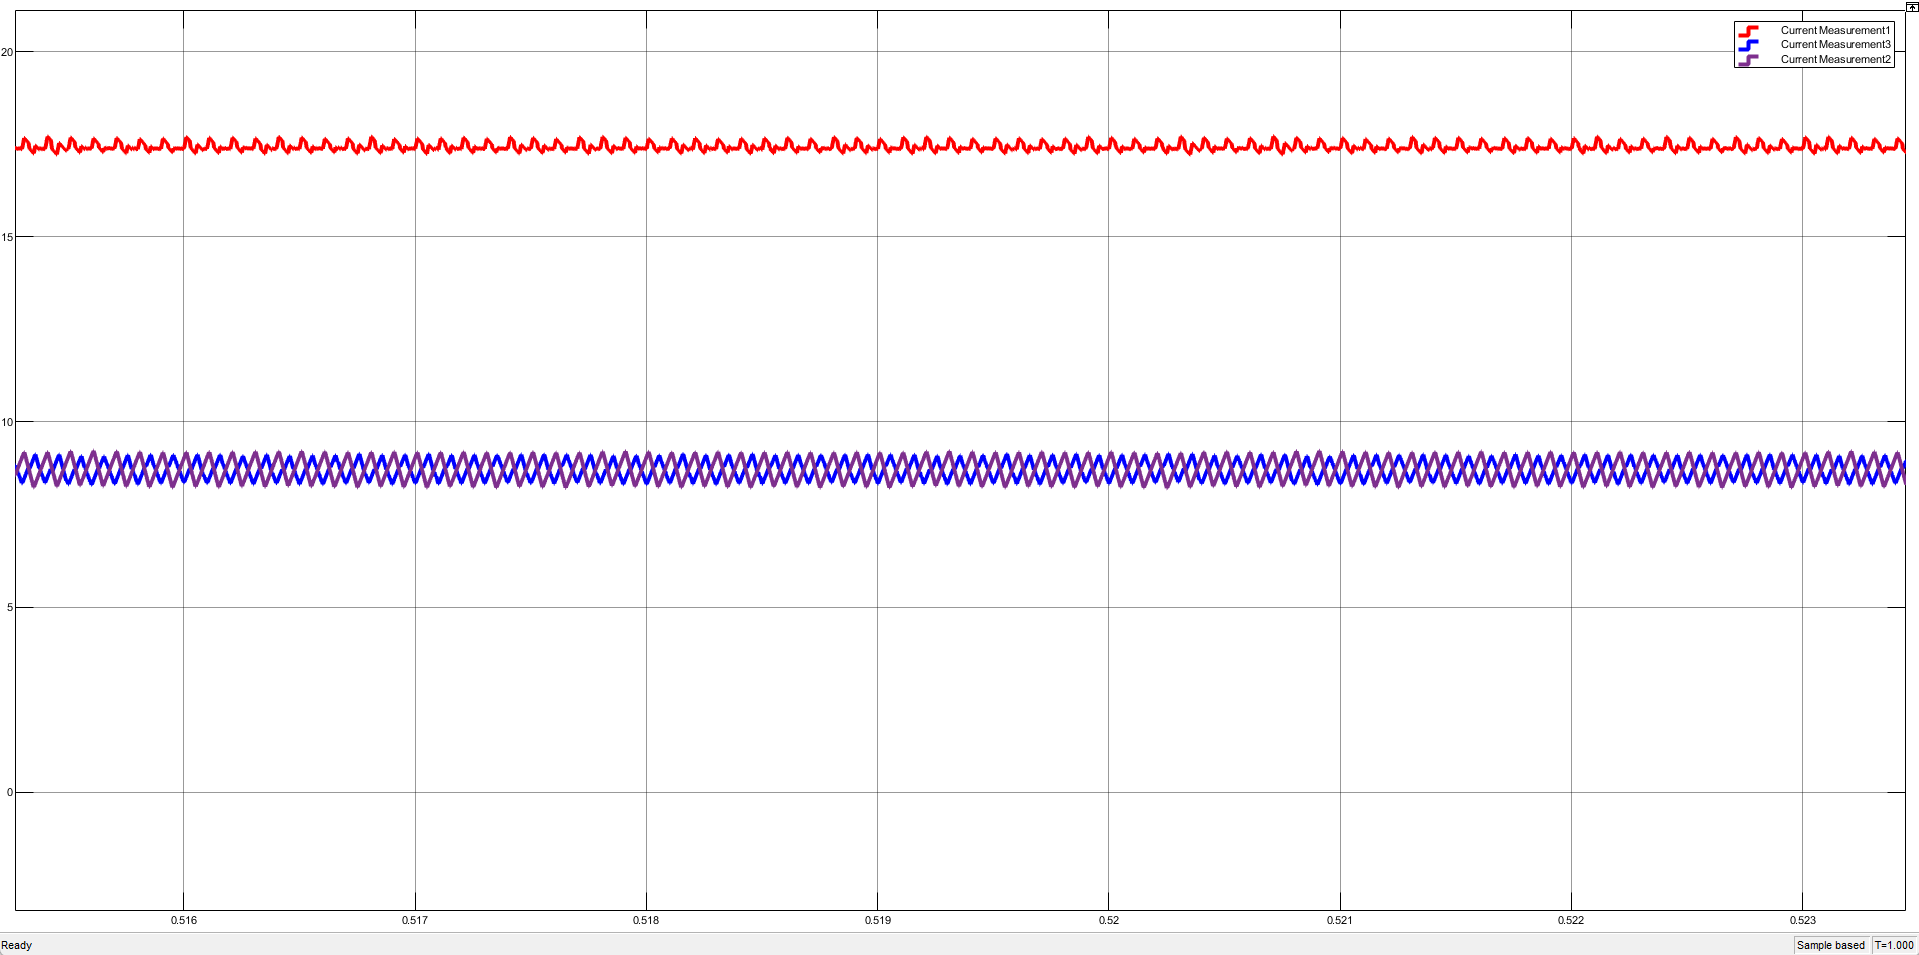
\includegraphics[width=0.9\textwidth]{Figures/5.1.60.png}
    \caption{Input total current, inductor current 1, inductor current 2 at string 2.}
    \label{fig:input total current, inductor current 1, inductor current 2 zoom at no shading at interleaved string at string 2}
\end{figure}
\begin{figure}[H]
    \centering
    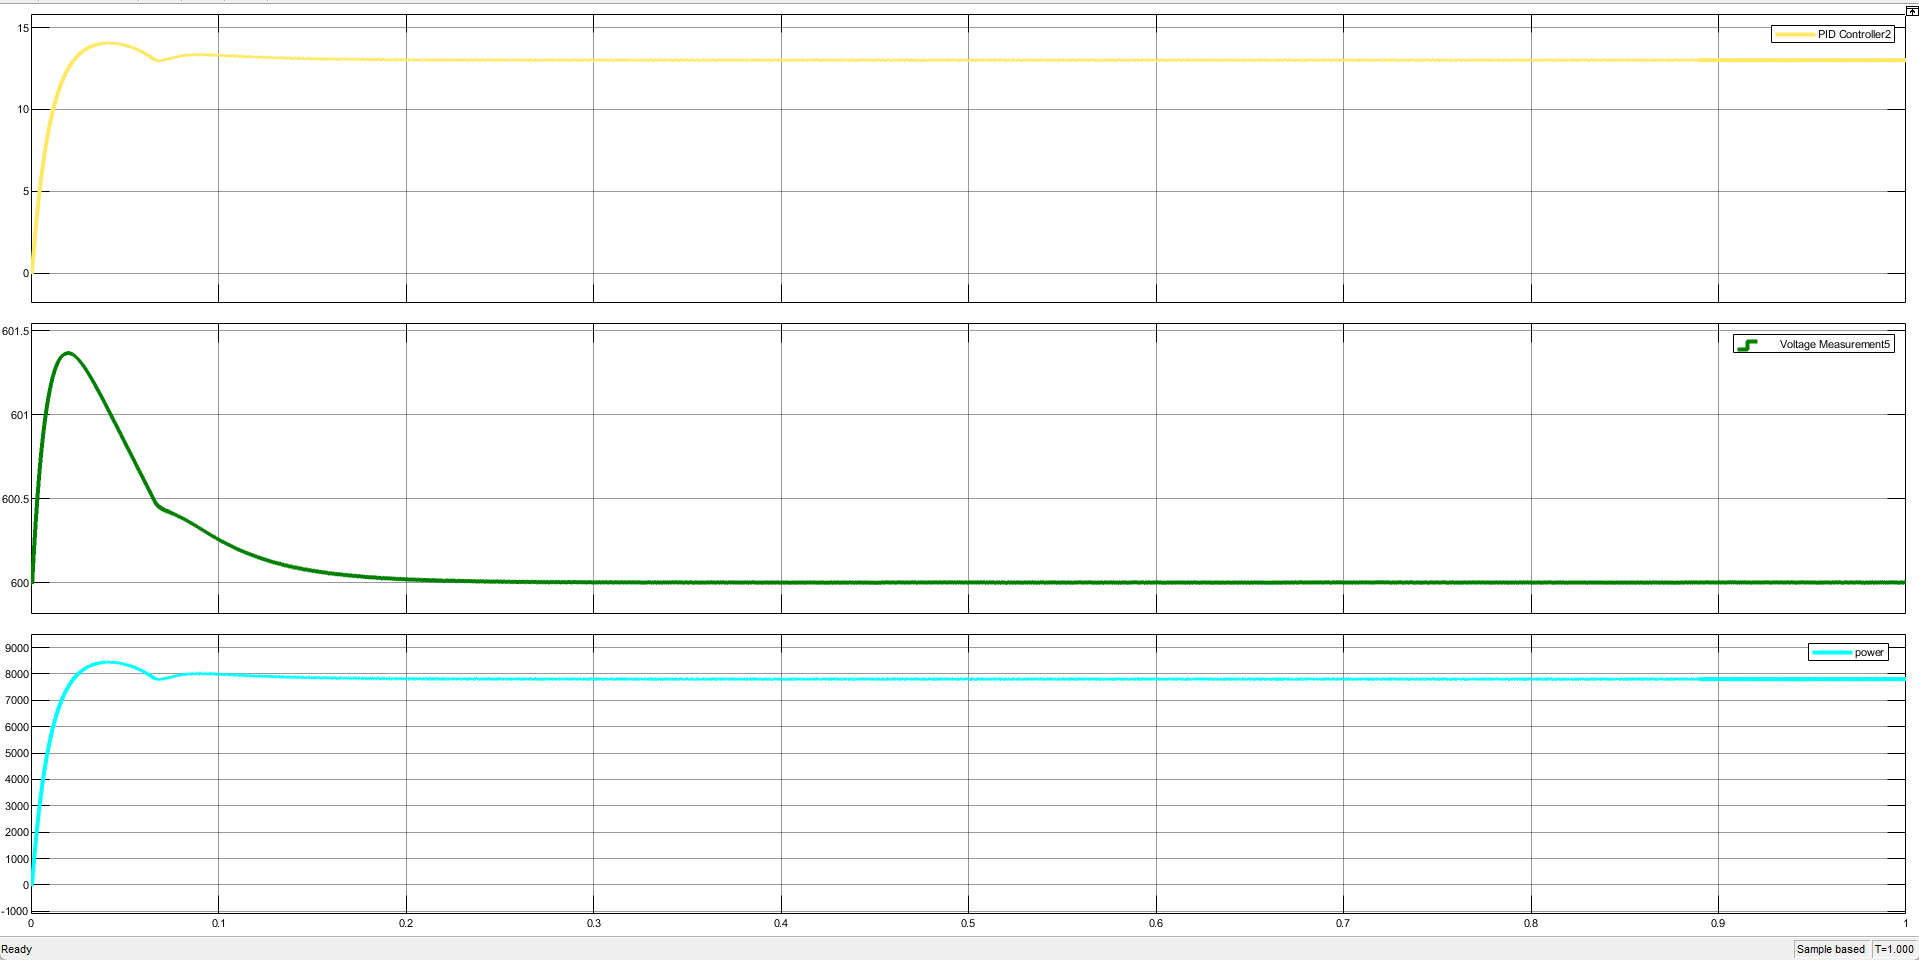
\includegraphics[width=0.9\textwidth]{Figures/5.1.61.png}
    \caption{Output current, voltage, power of interleaved string.}
    \label{fig:output current, voltage, power at no shading at interleaved string}
\end{figure}

\section{DC Buck-Boost Converter (High Ratings)}

\subsection{Open-Loop System Model (with Resistive Load)}

In the open-loop mode, a fixed duty cycle is applied to control the switching device without any feedback mechanism. Consequently, the output voltage depends solely on the input voltage, duty cycle, and circuit parameters. The output voltage follows the conventional buck--boost converter\cite{mohan2003}:

\begin{equation}
V_{out}=\frac{D\,V_{in}}{1-D}
\end{equation}

\subsubsection{Simulation Model}

\begin{figure}[H]
    \centering
    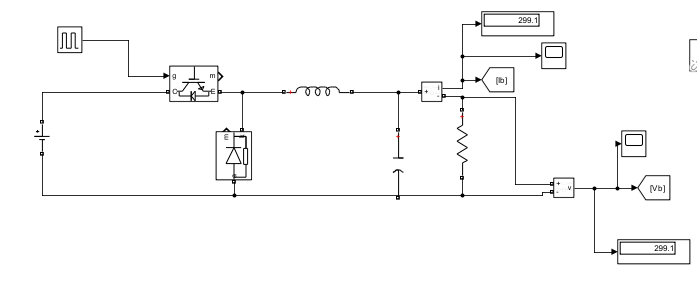
\includegraphics[width=0.85\textwidth]{Figures/2.png}
    \caption{Open-loop Two-Quadrant Chopper with Resistive Load}
    \label{fig:open_loop_resistor}
\end{figure}

\subsubsection{Results}

The converter performance was evaluated using different duty-cycle values.

\begin{itemize}
    \item Duty Cycle $D=0.5$
    \begin{figure}[H]
    \centering
    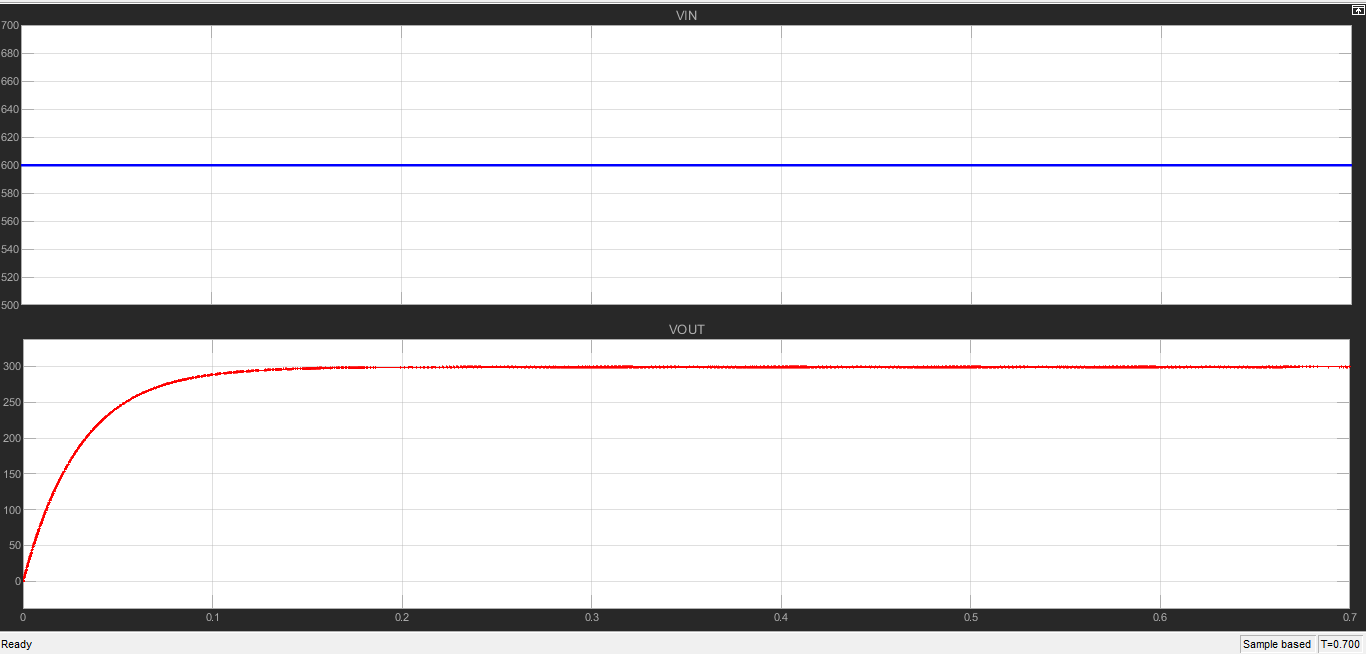
\includegraphics[width=0.85\textwidth]{Figures/0.5.png}
    \caption{Input and Output Voltage for duty cycle = 0.5}
    \label{fig:open_loop_resistor}
\end{figure}
    \item Duty Cycle $D=0.7$
    \begin{figure}[H]
    \centering
    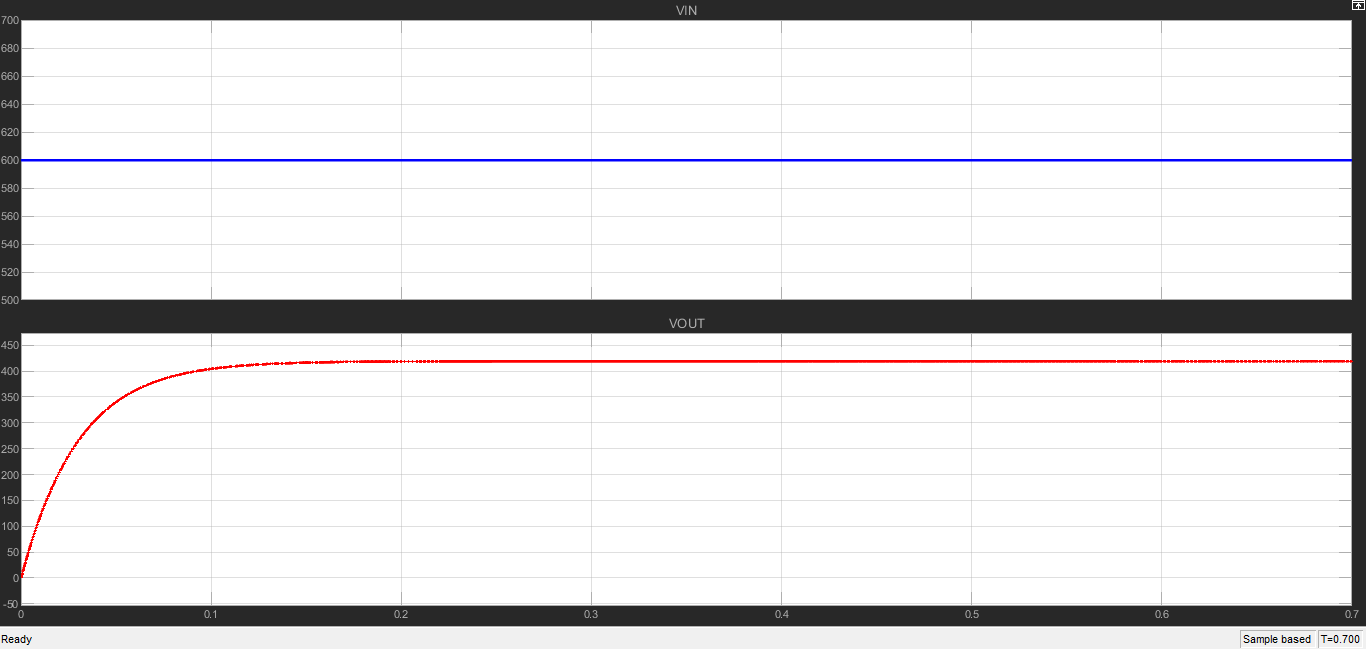
\includegraphics[width=0.85\textwidth]{Figures/0.7.png}
    \caption{Input and Output Voltage for duty cycle = 0.7}
    \label{fig:open_loop_resistor}
\end{figure}
    
\end{itemize}

%%%%%%%%%%%%%%%%%%%%%%%%%%%%%%%%%%%%%%%%%%%%%%%%%%%%%%%%%%

\subsection{Open-Loop System Model (Battery Modeled as an RC Load with CC--CV Control)}

In this configuration, the battery is represented by an equivalent RC circuit while the converter still operates in open-loop mode using a fixed duty cycle. The output voltage continues to follow the buck--boost converter equation:

\begin{equation}
V_{out}=\frac{D\,V_{in}}{1-D}
\end{equation}

\subsubsection{Simulation Model}

\begin{figure}[H]
    \centering
    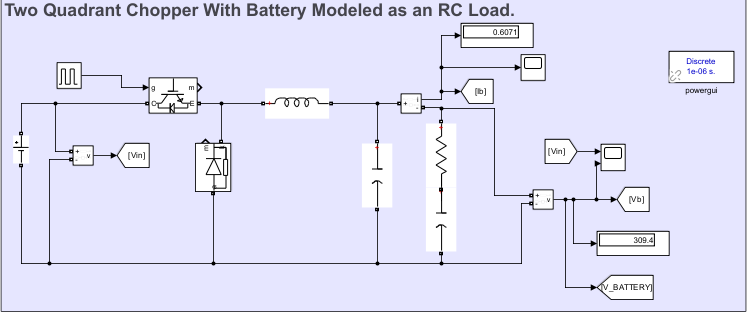
\includegraphics[width=0.85\textwidth]{Figures/3.png}
    \caption{Open-loop Two-Quadrant Chopper with RC Battery Model}
    \label{fig:open_loop_rc}
\end{figure}
\newpage
\subsubsection{Results}

The converter performance was evaluated using different duty-cycle values.

\begin{itemize}
    \item Duty Cycle $D=0.5$
    \begin{figure}[H]
    \centering
    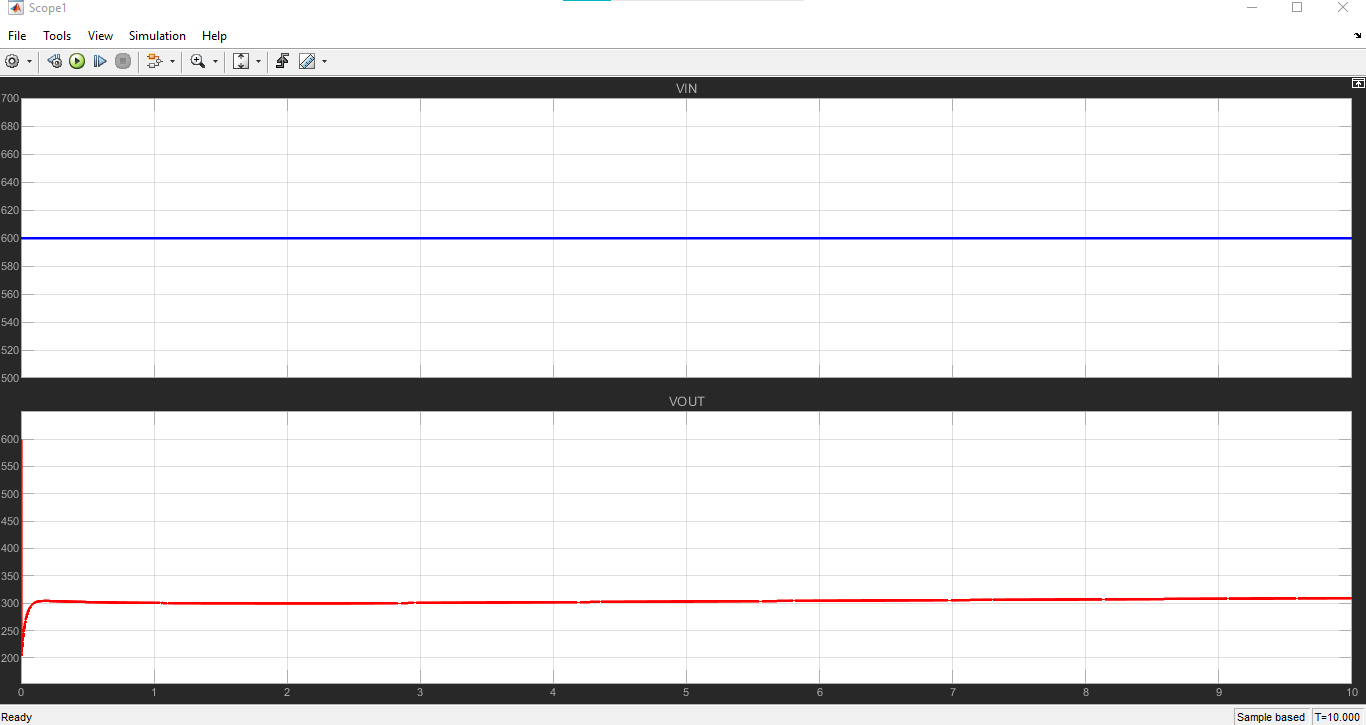
\includegraphics[width=0.85\textwidth]{Figures/2Q/D50 RC.png}
    \caption{Input and Output Voltage for duty cycle = 0.5}
    \label{fig:open_loop_resistor}
\end{figure}
    \item Duty Cycle $D=0.7$
    \begin{figure}[H]
    \centering
    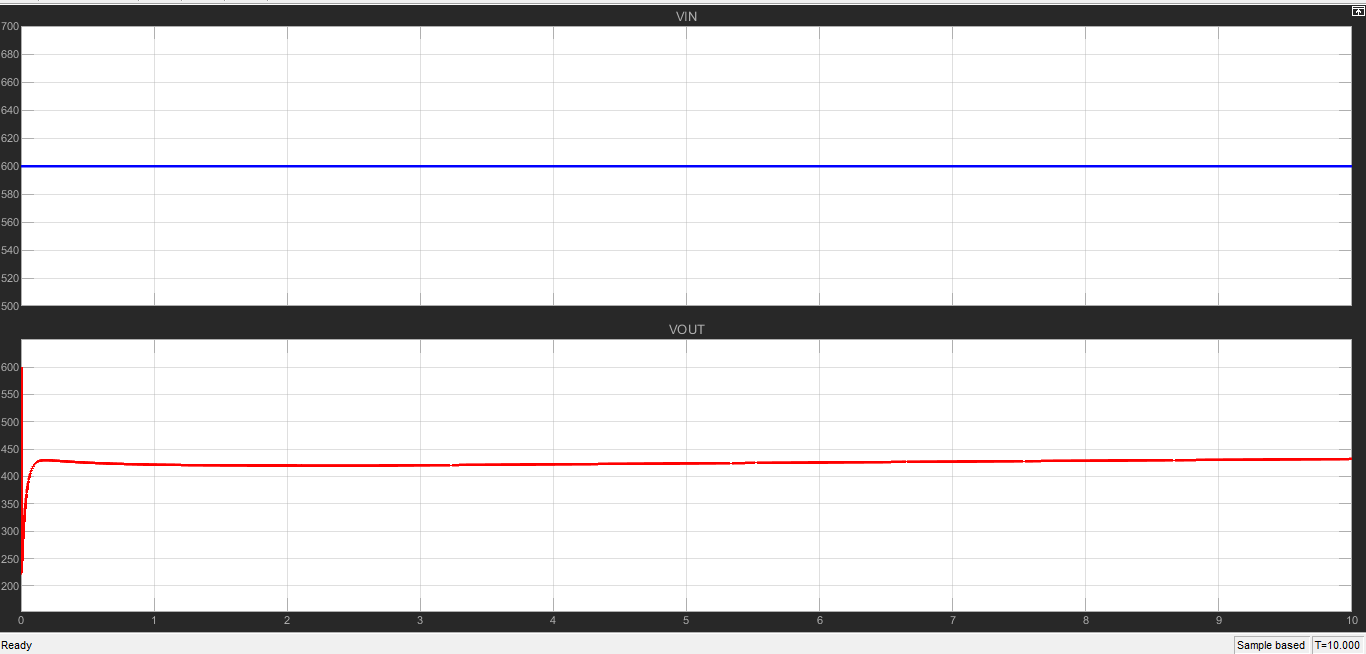
\includegraphics[width=0.85\textwidth]{Figures/D70RC.png}
    \caption{Input and Output Voltage for duty cycle = 0.7}
    \label{fig:open_loop_resistor}
\end{figure}
    
\end{itemize}



%%%%%%%%%%%%%%%%%%%%%%%%%%%%%%%%%%%%%%%%%%%%%%%%%%%%%%%%%%

\subsection{Closed-Loop System (Battery Modeled as an RC Load with CC--CV Control)}

To represent the battery charging process more realistically, the ideal battery was replaced with an equivalent electrical model consisting of a resistor and capacitor connected in series (RC model). The capacitor represents the battery storage capacity, whereas the resistor models the internal resistance.
\newpage
The charging behavior is governed by the RC time constant,

\begin{equation}
\tau=RC
\end{equation}

where

\[
R=1~\Omega,\qquad C=0.5~\mathrm{F}
\]

thus,

\[
\tau=0.5~\mathrm{s}
\]

%%%%%%%%%%%%%%%%%%%%%%%%%%%%%%%%%%%%%%%%%%%%%%%%%%%%%%%%%%

\subsubsection{Constant Current (CC) Stage}

Initially, the battery is charged using a constant current regulated by a PI current controller. During this stage, the battery voltage increases gradually according to the RC charging characteristics.

\begin{figure}[H]
    \centering
    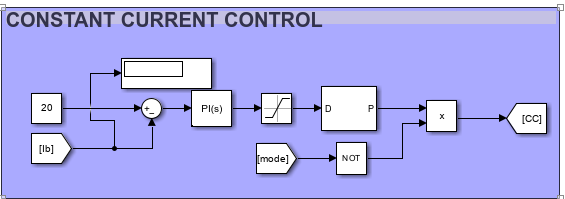
\includegraphics[width=0.8\textwidth]{Figures/cc.png}
    \caption{Constant Current Control}
    \label{fig:cc_control}
\end{figure}

%%%%%%%%%%%%%%%%%%%%%%%%%%%%%%%%%%%%%%%%%%%%%%%%%%%%%%%%%%

\subsubsection{Constant Voltage (CV) Stage}

Once the battery voltage reaches the predefined limit of approximately $570~\mathrm{V}$, the control system automatically switches to the voltage PI controller. During this stage, the battery voltage is maintained at the reference value while the charging current gradually decreases toward zero, indicating the completion of the charging process.

\begin{figure}[H]
    \centering
    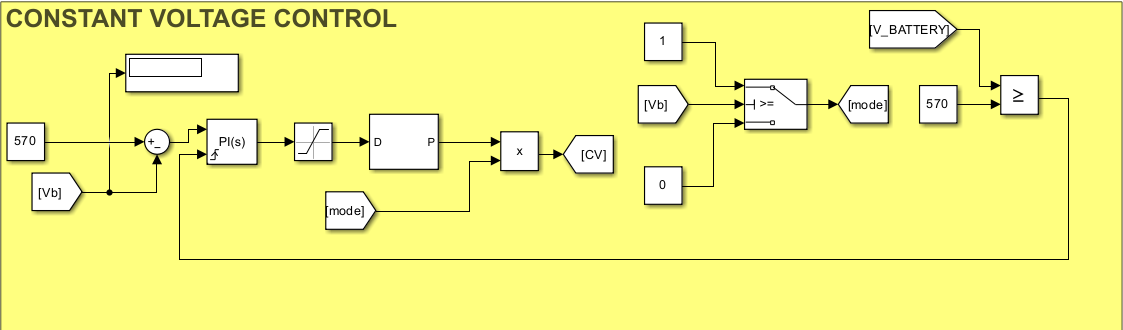
\includegraphics[width=0.8\textwidth]{Figures/cv.png}
    \caption{Constant Voltage Control}
    \label{fig:cv_control}
\end{figure}

%%%%%%%%%%%%%%%%%%%%%%%%%%%%%%%%%%%%%%%%%%%%%%%%%%%%%%%%%%

\subsubsection{Results}

\paragraph{CC--CV Charging Profile}

\begin{figure}[H]
    \centering
    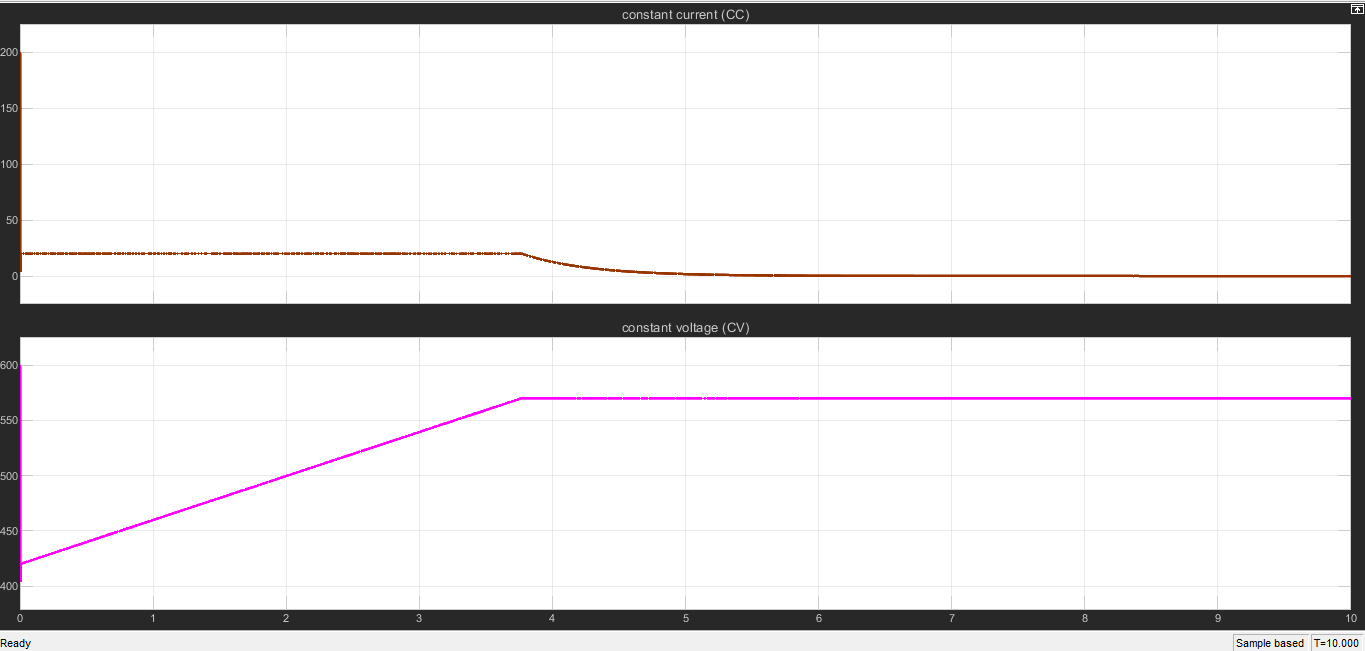
\includegraphics[width=0.85\textwidth]{Figures/cc-cv.png}
    \caption{CC--CV Charging Profile of the Energy Storage System}
    \label{fig:cc_cv_profile}
\end{figure}

The charging profile illustrates the two-stage charging strategy. During the Constant Current (CC) stage, the controller maintains a fixed charging current to maximize charging efficiency. Once the battery voltage reaches the safety threshold, the controller transitions smoothly to the Constant Voltage (CV) stage. During this phase, the charging current decreases gradually while maintaining the battery voltage at its reference value, ensuring safe and reliable battery charging.

%%%%%%%%%%%%%%%%%%%%%%%%%%%%%%%%%%%%%%%%%%%%%%%%%%%%%%%%%%

\paragraph{Voltage Regulation}

\begin{figure}[H]
    \centering
    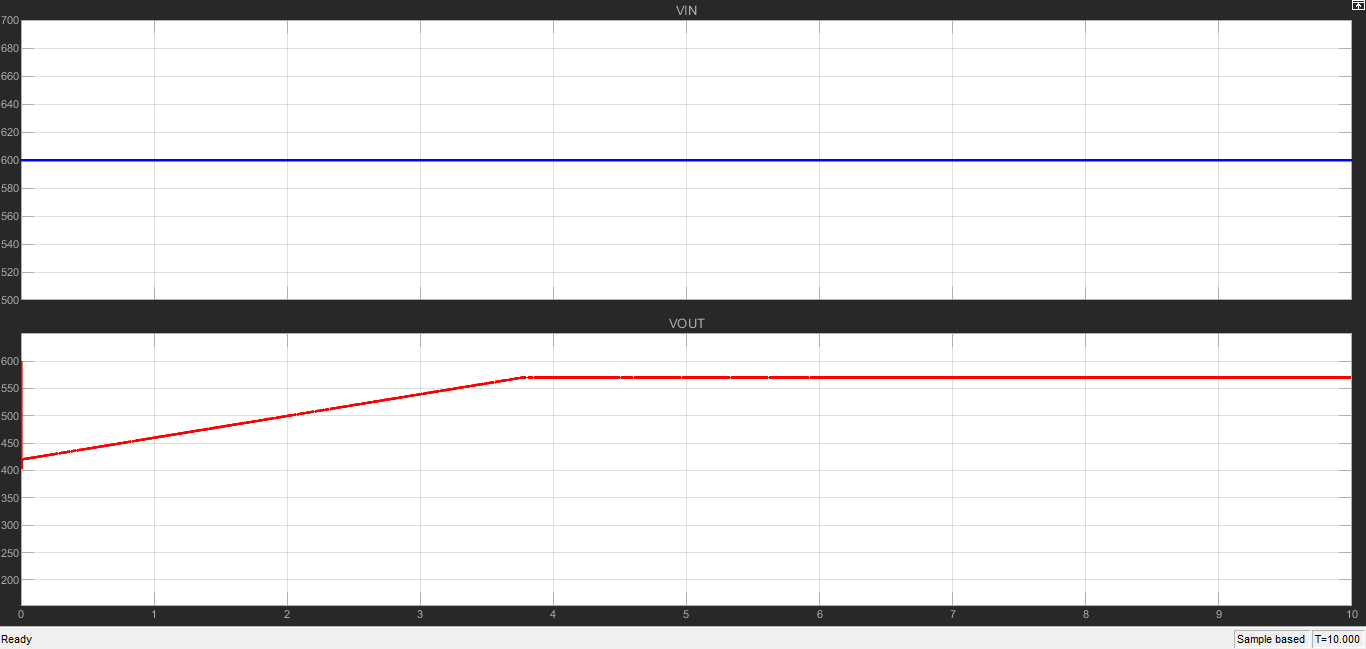
\includegraphics[width=0.85\textwidth]{Figures/v.png}
    \caption{Voltage Conversion from the DC Bus to the Energy Storage System}
    \label{fig:voltage_regulation}
\end{figure}

The waveform demonstrates the voltage conversion from the 600 V DC bus to the regulated battery charging voltage of approximately 570 V. The controller accurately maintains this voltage level during the Constant Voltage stage, ensuring that the battery is charged safely while preventing over-voltage conditions.
\section{Buck Converter Battery Charging Simulation (High Ratings)} % This will display as 5.3 Buck Converter Battery Charging Simulation

\subsection{System Parameters} % This becomes 5.3.1
The simulation model consists of a DC-link buck converter supplying a series $RC$ load, which models the electrical behavior of a battery.

\begin{table}[h!]
\centering
\caption{Simulation Configuration Parameters}
\label{tab:parameters}
\begin{tabular}{ll}
\toprule
\textbf{Parameter} & \textbf{Value} \\ 
\midrule
Input Voltage ($V_{dc}$) & $600\text{ V}$ \\
Filter Inductor ($L$) & $30\text{ mH}$ \\
Output Capacitor ($C_{out}$) & $200\ \mu\text{F}$ \\
Equivalent Load Resistance ($R$) & $1\ \Omega$ \\
Equivalent Load Capacitance ($C$) & $0.5\text{ F}$ \\
\bottomrule
\end{tabular}
\end{table}

\subsection{Control Strategy} % This becomes 5.3.2
The system implements a dual-mode closed-loop PID control strategy to replicate a standard Constant Current / Constant Voltage (CC/CV) battery charging profile.

\begin{itemize}
    \item \textbf{Mode 1: Constant Current (CC) Mode}
    \begin{itemize}
        \item \textbf{Condition:} Measured voltage $V_{out} < V_{ref}$ ($570\text{ V}$).
        \item \textbf{Operation:} The current loop PID regulates the charging current to a fixed reference of $20\text{ A}$.
    \end{itemize}
    
    \item \textbf{Mode 2: Constant Voltage (CV) Mode}
    \begin{itemize}
        \item \textbf{Condition:} Measured voltage $V_{out} \ge V_{ref}$ ($570\text{ V}$).
        \item \textbf{Operation:} Control switches to the voltage loop PID, clamping the output at $570\text{ V}$ while the current naturally decays.
    \end{itemize}
\end{itemize}

\begin{figure}[h!]
    \centering
    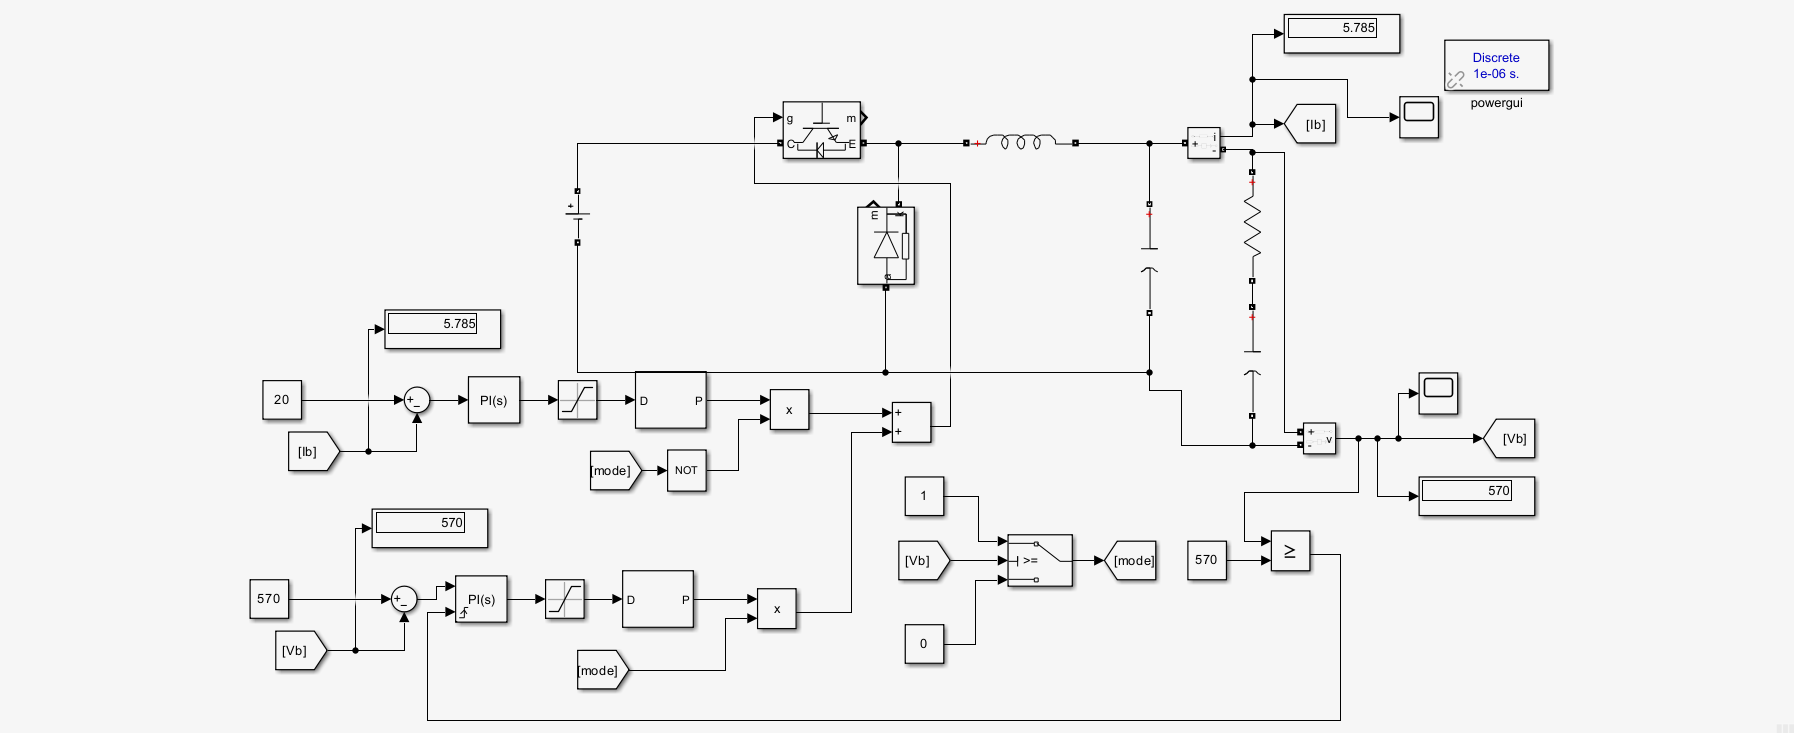
\includegraphics[width=0.8\textwidth]{Figures/volt.png} 
    \caption{MATLAB/Simulink Control Mode Boundary Analysis}
    \label{fig:control_boundary}
\end{figure}

\subsection{Simulation Results \& Discussion} % This becomes 5.3.3

\paragraph{Phase Analysis}
\begin{itemize}
    \item \textbf{Transient Phase (CC Mode):} Initially, the battery voltage is below $570\text{ V}$. The current PID loop successfully regulates the charging current to $20\text{ A}$, causing the battery capacitor to charge linearly.
\end{itemize}

\begin{figure}[h!]
    \centering
    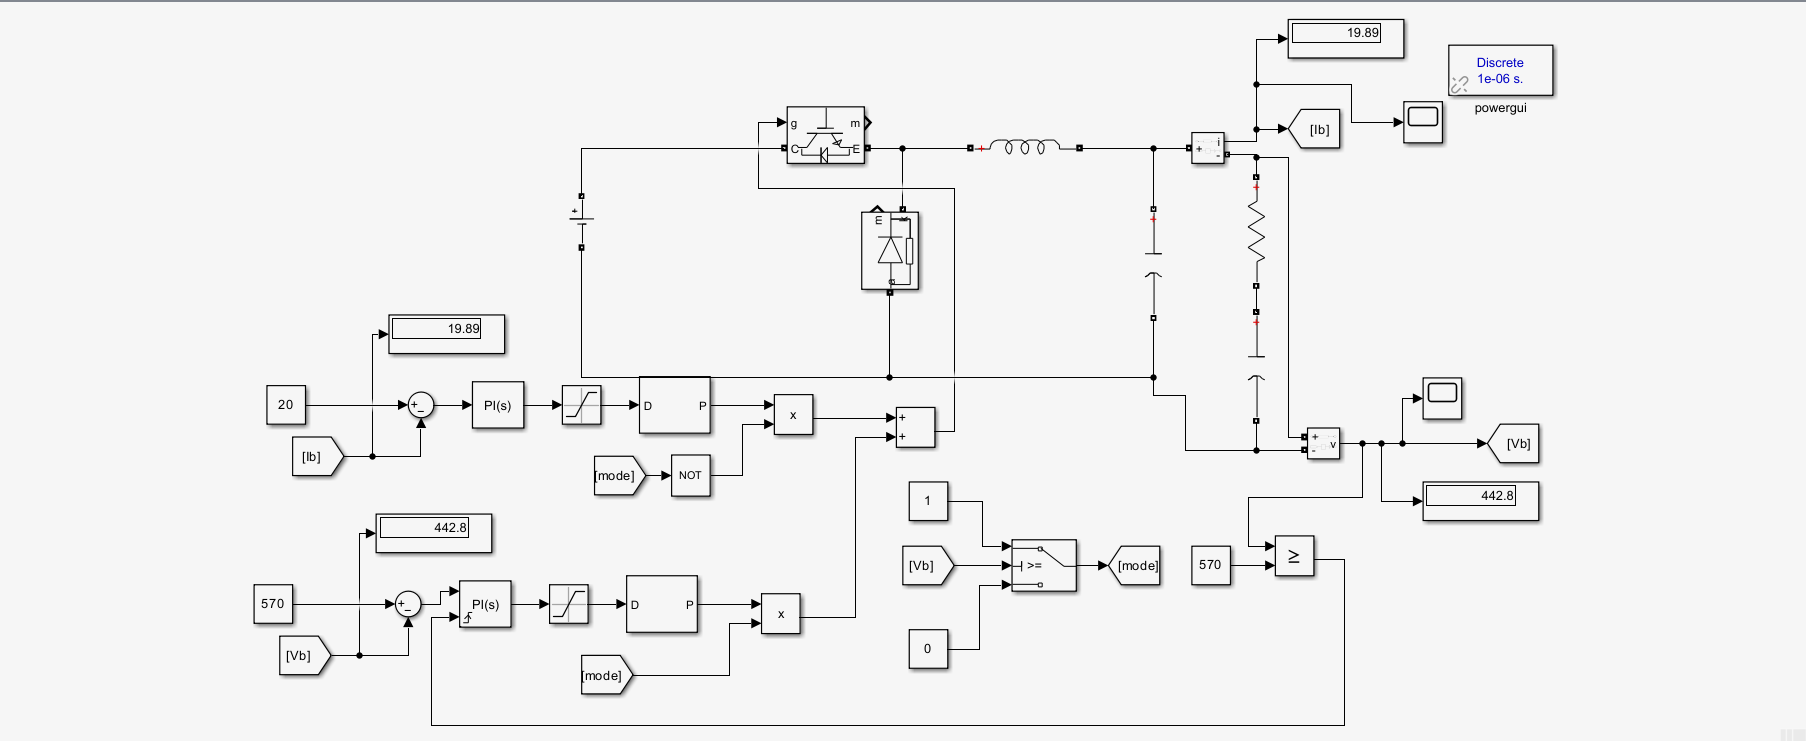
\includegraphics[width=0.8\textwidth]{Figures/current.png} 
    \caption{MATLAB/Simulink Current Response Waveform}
    \label{fig:current_waveform}
\end{figure}

\begin{itemize}
    \item \textbf{Transition Phase:} Once the battery voltage reaches the $570\text{ V}$ threshold, the control logic smoothly transitions from current control to voltage control.
    \item \textbf{Steady-State Phase (CV Mode):} The voltage PID loop stabilizes the output at $570\text{ V}$. As the battery approaches full charge, the current exponentially decays toward zero, preventing overcharging.
\end{itemize}

\paragraph{Scope Observations}
\begin{itemize}
    \item \textbf{Current Scope ($I$):} Shows a constant $20\text{ A}$ plateau during the CC phase, followed by a sharp exponential decay toward $0\text{ A}$ once CV mode is activated.
    
    \item \textbf{Voltage Scope ($V$):} Displays a linear voltage rise during the CC phase, which smoothly flattens out and stabilizes precisely at the $570\text{ V}$ threshold as the controller switches modes.
\end{itemize}

\begin{figure}[h!]
    \centering
    \begin{minipage}{0.48\textwidth}
        \centering
        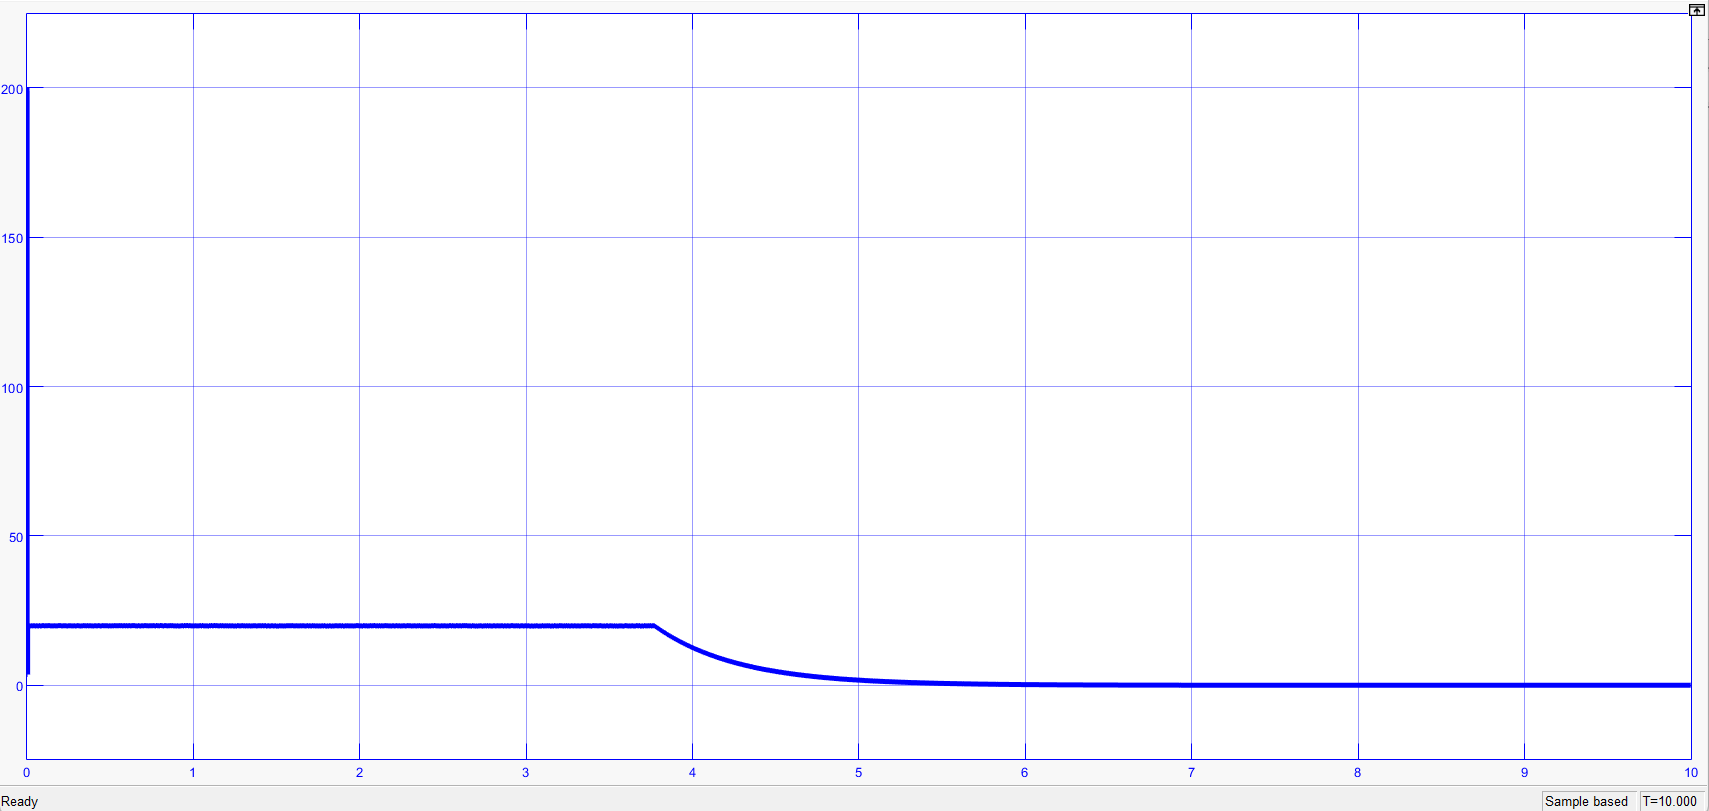
\includegraphics[width=\textwidth]{Figures/current scope.png} 
        \caption{Charging Current ($I$)}
        \label{fig:current_scope}
    \end{minipage}
    \hfill
    \begin{minipage}{0.48\textwidth}
        \centering
        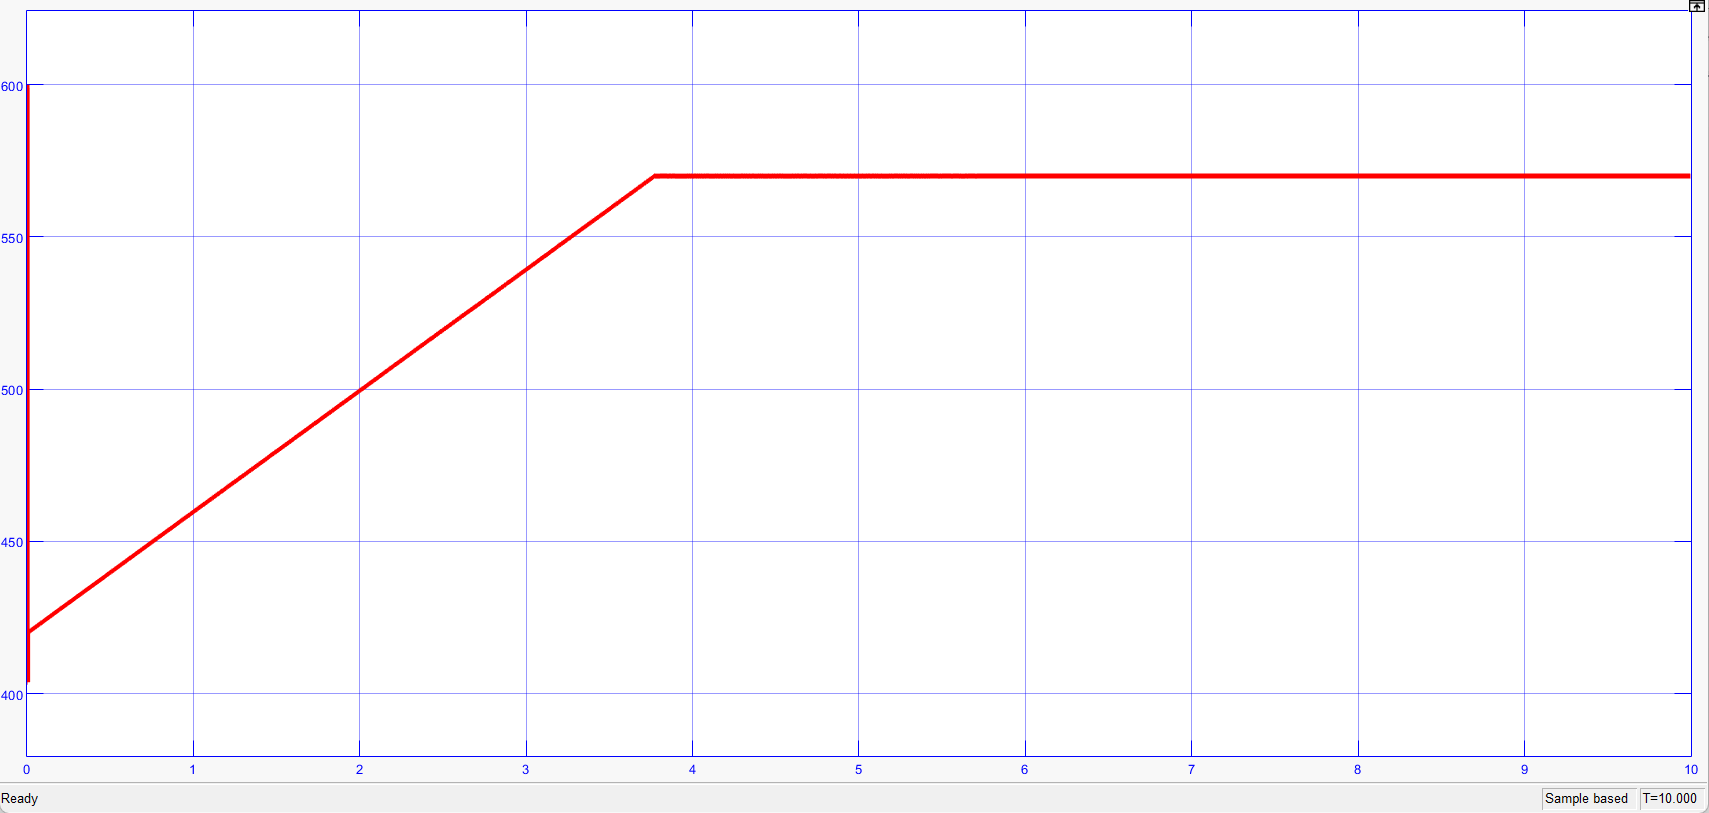
\includegraphics[width=\textwidth]{Figures/volt scope.png}
        \caption{Battery Voltage ($V$)}
        \label{fig:voltage_scope}
    \end{minipage}
\end{figure}
\newpage
\subsection{Conclusion} % This becomes 5.3.4
The closed-loop buck converter successfully demonstrates automated CC/CV battery charging. The transition between the current-controlled phase ($20\text{ A}$) and the voltage-controlled phase ($570\text{ V}$) is stable, ensuring safe and efficient energy transfer to the $RC$ battery model.

\section{Simulation of the System Tied with Grid}
the Photovoltaic (PV) system and the Electric Vehicle (EV) charger are connected directly to the local utility grid. The grid acts as an infinite source and sink for power.
\vspace{0.5pt}
\noindent\textbf{Key Advantages of Grid-Tied Topologies:}
\begin{description}
    \item[\textbf{Bidirectional Power Flow and Revenue Generation:}] 
    Excess solar energy generated during peak ambient sunlight hours can be seamlessly fed back into the local utility distribution network through net metering frameworks. This mechanism allows system owners to accumulate utility credits or direct revenue, substantially accelerating the capital payback period of the infrastructure installation.
    
    \item[\textbf{Elimination of Intermittency Risks:}] 
    Because the utility grid serves as a continuous, infinite-bus backup supply asset, Electric Vehicle (EV) charging operations are completely isolated from disruptions caused by transient weather alterations, nighttime intervals, or rapid step-drops in local solar irradiance. Consequently, the system circumvents the operational requirement for strict real-time load matching.
    
    \item[\textbf{Reduced Capital Expenditure:}] 
    Eliminating a dedicated stationary electrochemical battery storage bank dramatically lowers the initial structural capital investment, minimizes total system topology complexity, and completely avoids the spatial, ventilation, and safety engineering requirements of large battery containment facilities.
    
    \item[\textbf{Support for Grid Services (V2G Integration):}] 
    When configured with a bidirectional power electronics conversion stage, the system becomes fully Vehicle-to-Grid (V2G) capable. The interconnected EV battery string can then operate as a dynamic decentralized energy storage asset, providing active peak-shaving, load-leveling, or frequency regulation services back to the utility grid during parked cycles.
    
    \item[\textbf{Lower Maintenance and Elevated System Efficiency:}] 
    By operating without intermediate chemical energy storage components, the system cuts down on unnecessary power conversion stages—completely eliminating the extra $I^2R$ and switching losses typically associated with localized battery charging. This direct transmission line interface reduces long-term maintenance overhead, as static grid-tied inverters exhibit significantly longer operational life cycles than chemical battery cells.
\end{description}

\newpage
\subsection{Inverter Tied with Grid}
\subsubsection{Why we need Transformation from abc to dq}
In a three-phase grid-tied inverter system, the voltages and currents are inherently sinusoidal AC signals in the stationary $abc$ reference frame. Directly controlling these variables using standard Proportional-Integral (PI) controllers introduces a fundamental limitation: due to the finite gain of the integrator at non-zero frequencies, a standard PI controller cannot track a sinusoidal reference with zero steady-state error, resulting in persistent phase lag and amplitude attenuation.

To overcome this, the Park clark Transformation ($abc \to dq$) is utilized to map the three-phase AC variables into a synchronous reference frame rotating at the grid angular frequency $\omega$. In this rotating frame, balanced fundamental AC signals appear as stationary DC quantities during steady-state conditions, enabling PI controllers to achieve infinite open-loop gain at DC and completely eliminate steady-state error\cite{singh2020}.

\subsection{Clark Transformation}
\begin{itemize}
    \item \textbf{Clarke Transform}, also known as alpha-beta transformation.
    \item \textbf{Clarke} transforms \textbf{variable three-phase} ac ($a,b,c$) in \textbf{stationary frame} to \textbf{variable two-phase} ac ($\alpha,\beta$) \textbf{in stationary frame too}.
\end{itemize}

\vspace{0.5cm}

\subsection*{1. Vector Frame Representation}

The transformation maps three spatial vectors separated by $120^\circ$ into an orthogonal two-axis system ($\alpha \perp \beta$). 

\begin{center}
    \begin{tabular}{c c c}
        \textbf{Three-Phase Stationary Frame ($abc$)} & & \textbf{Two-Phase Stationary Frame ($\alpha\beta$)} \\
        \begin{minipage}{0.4\textwidth}
            \centering
            % Reference equations for abc system
            \begin{equation*}
                \boxed{
                \begin{aligned}
                    v_a &= V_M \sin(\omega t) \\
                    v_b &= V_M \sin(\omega t - 120^\circ) \\
                    v_c &= V_M \sin(\omega t + 120^\circ)
                \end{aligned}
                }
            \end{equation*}
        \end{minipage}
        & $\Longrightarrow$ &
        \begin{minipage}{0.4\textwidth}
            \centering
            % Reference equations for alpha-beta system
            \begin{equation*}
                \boxed{
                \begin{aligned}
                    v_\alpha &= V_M \sin(\omega t) \\
                    v_\beta &= V_M \sin(\omega t - 90^\circ)
                \end{aligned}
                }
            \end{equation*}
        \end{minipage}
    \end{tabular}
\end{center}

\begin{center}
    \textbf{The equivalent sum should be the same in two cases}
\end{center}
\begin{figure}[H]
    \centering
    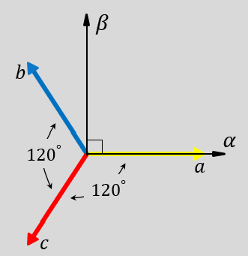
\includegraphics[width=0.5\textwidth]{Figures/5.4.1.png}
    \caption{Clark transformation.}
    \label{clark transformation}
\end{figure}
\begin{figure}[H]
    \centering
    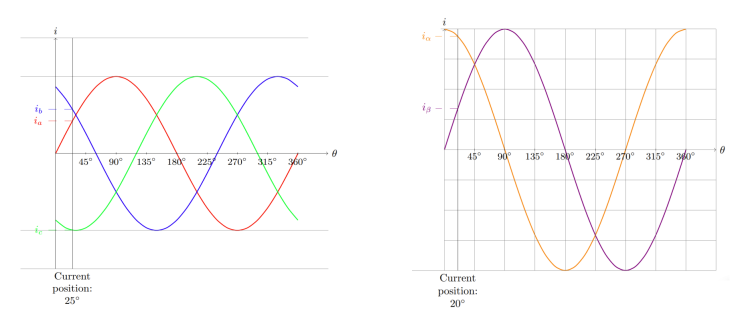
\includegraphics[width=1.1\textwidth]{Figures/5.4.2.png}
    \caption{Clark transformation waveform.}
    \label{clark transformation graph}
\end{figure}

\begin{center}
        \begin{equation*}
            \left[\begin{array}{c}
                v_\alpha \\[6pt]
                v_\beta \\[6pt]
                v_0
            \end{array}\right]
            = \frac{2}{3}
            \left[\begin{array}{ccc}
                1 & -\dfrac{1}{2} & -\dfrac{1}{2} \\[10pt]
                0 & \dfrac{\sqrt{3}}{2} & -\dfrac{\sqrt{3}}{2} \\[10pt]
                \dfrac{1}{2} & \dfrac{1}{2} & \dfrac{1}{2}
            \end{array}\right]
            \left[\begin{array}{c}
                v_a \\[6pt]
                v_b \\[6pt]
                v_c
            \end{array}\right]
        \end{equation*}
\end{center}
\newpage
\subsection{Park Transformation}
\begin{itemize}
    \item \textbf{Park Transform}, also known as d-q transformation.
    \item \textbf{Park} transforms \textbf{variable three-phase} ac ($a,b,c$) in \textbf{stationary frame} to \textbf{constant two-phase} ac ($d,q$) \textbf{in in rotating frame}.
\end{itemize}
\begin{figure}[H]
    \centering
    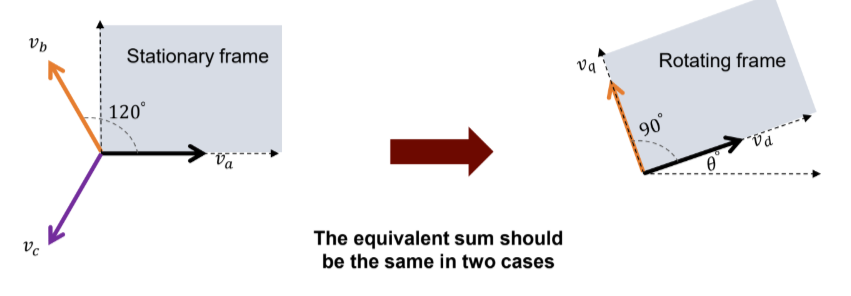
\includegraphics[width=1.1\textwidth]{Figures/5.4.3.png}
    \caption{Park transformation.}
    \label{park transformation graph}
\end{figure}

\begin{equation}
    \left[\begin{array}{c}
        v_d \\[6pt]
        v_q
    \end{array}\right]
    =
    \left[\begin{array}{cc}
        \cos(\theta)  & \sin(\theta) \\[6pt]
        -\sin(\theta) & \cos(\theta)
    \end{array}\right]
    \left[\begin{array}{c}
        v_\alpha \\[6pt]
        v_\beta
    \end{array}\right]
\end{equation}

\subsection{Park Clark Transformation}
\begin{equation}
    \left[\begin{array}{c}
        v_d \\[6pt]
        v_q
    \end{array}\right]
    =
    \frac{2}{3}
    \left[\begin{array}{ccc}
        \cos(\theta)  & \cos\!\left(\theta - \dfrac{2\pi}{3}\right) & \cos\!\left(\theta + \dfrac{2\pi}{3}\right) \\[14pt]
        \sin(\theta)  & \sin\!\left(\theta - \dfrac{2\pi}{3}\right) & \sin\!\left(\theta + \dfrac{2\pi}{3}\right)
    \end{array}\right]
    \left[\begin{array}{c}
        v_a \\[6pt]
        v_b \\[6pt]
        v_c
    \end{array}\right]
\end{equation}

\subsection{PLL(phase locked loop)}
In grid-tied power electronic interfaces—such as the three-phase static inverter topology connected to a photovoltaic (PV) array—precise synchronization with the local utility network is critical. To achieve this synchronization, a Phase-Locked Loop (PLL) is utilized as the primary control block to continuously track the utility grid's voltage vector profile. 

\begin{figure}[H]
    \centering
    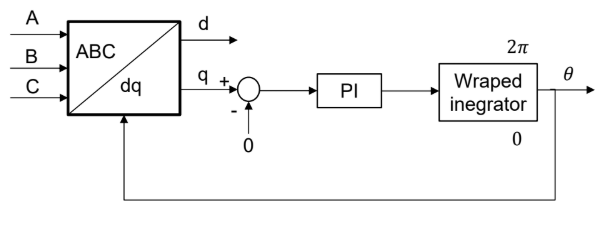
\includegraphics[width=1.1\textwidth]{Figures/5.4.4.png}
    \caption{PLL control circuit.}
    \label{PLL}
\end{figure}

\subsection{Control Circuit}
The aim is to control the converter current (act as controlled current source) to achieve certain purpose like , injecting active power (renewable sources), injecting reactive power (support grid voltage), or controlling active and reactive power (grid quality )
\begin{figure}[H]
    \centering
    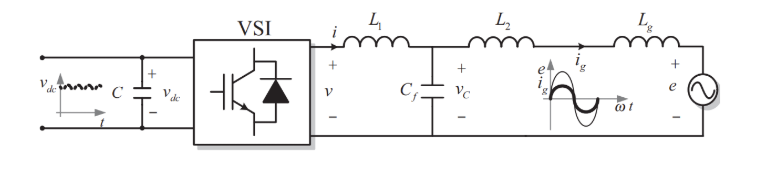
\includegraphics[width=1.1\textwidth]{Figures/5.4.20.png}
    \caption{Grid connected VSC.}
    \label{Grid connected VSC}
\end{figure}
\begin{figure}[H]
    \centering
    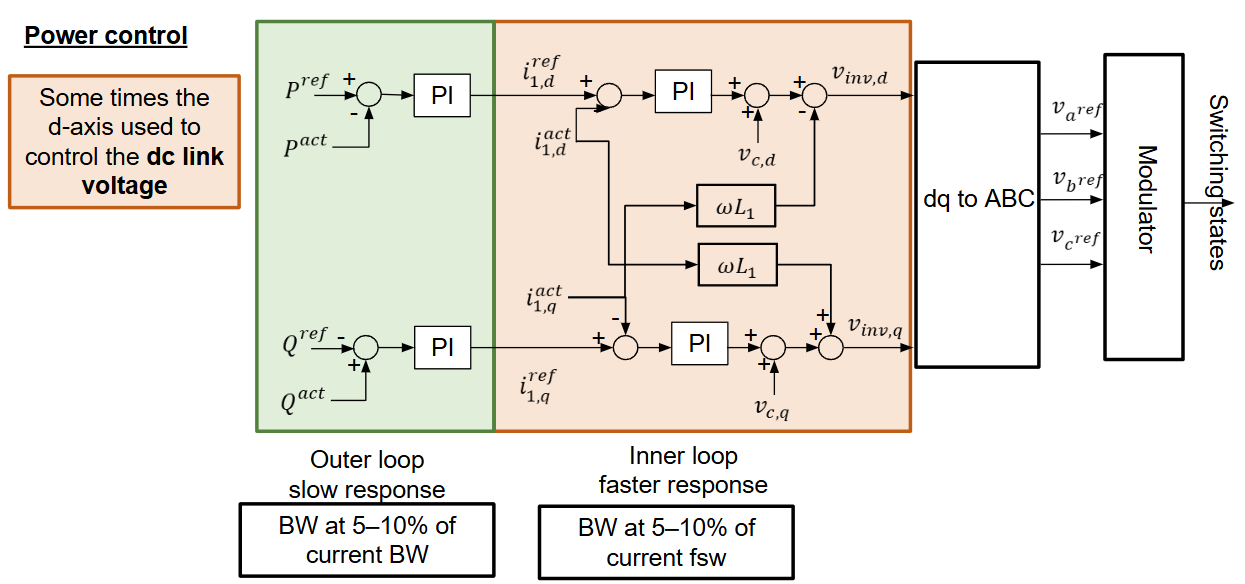
\includegraphics[width=1.1\textwidth]{Figures/5.4.21.png}
    \caption{Control diagram.}
    \label{control diagram.}
\end{figure}

% ==========================================================
% SECTION: ACTIVE AND REACTIVE POWER IN THE dq FRAME
% ==========================================================

\subsection{Active and Reactive Power Modeling in the Synchronous $d\text{-}q$ Frame}

In a three-phase system, the instantaneous active power ($P$) and reactive power ($Q$) can be expressed directly using the orthogonal components of the synchronous rotating $d\text{-}q$ reference frame. Using the amplitude-invariant transformation convention, the comprehensive power expressions are defined as follows:

\begin{equation}
    P = \frac{3}{2} \left( v_d i_d + v_q i_q \right)
\end{equation}

\begin{equation}
    Q = \frac{3}{2} \left( v_q i_d - v_d i_q \right)
\end{equation}

Where $v_d, v_q$ represent the $d\text{-}q$ axis voltage components, and $i_d, i_q$ represent the corresponding $d\text{-}q$ axis current vectors injected into the grid interface.
\newpage
\subsubsection{ Power Control}

for balanced three phase voltage aligned with grid:
\begin{equation}
    v_q = 0
\end{equation}

Substituting $v_q = 0$ into the core power equations simplifies the expressions, yielding a highly desirable decoupled relationship:

\begin{equation}
    P = \frac{3}{2} v_d i_d \quad \longrightarrow \quad \text{Controlled directly via } i_d
\end{equation}

\begin{equation}
    Q = -\frac{3}{2} v_d i_q \quad \longrightarrow \quad \text{Controlled directly via } i_q
\end{equation}

\paragraph{Control Implications}
This mathematical simplification provides a foundational advantage for grid-tied inverter operation:
\begin{itemize}
    \item \textbf{Active Power Regulation ($P$):} Because the grid voltage $v_d$ is regulated to a constant value by the utility infrastructure, the instantaneous active power transfer becomes purely dependent on the direct-axis current component ($i_d$).
    \item \textbf{Reactive Power Regulation ($Q$):} Similarly, the instantaneous reactive power flow becomes decoupled and depends solely on adjusting the quadrature-axis current component ($i_q$). 
\end{itemize}
Consequently, the system can implement separate, independent PI tracking regulators for $i_d$ and $i_q$, allowing for concurrent optimization of active power extraction (e.g., maximizing PV output) and reactive power mitigation (achieving unity power factor or supporting grid voltage stability).

\subsection{Simulation of Inverter}
The goal is that the active power = 50000W , so Id = 100A

Note: The dc link must be more than phase to phase voltage at least double
\begin{figure}[H]
    \centering
    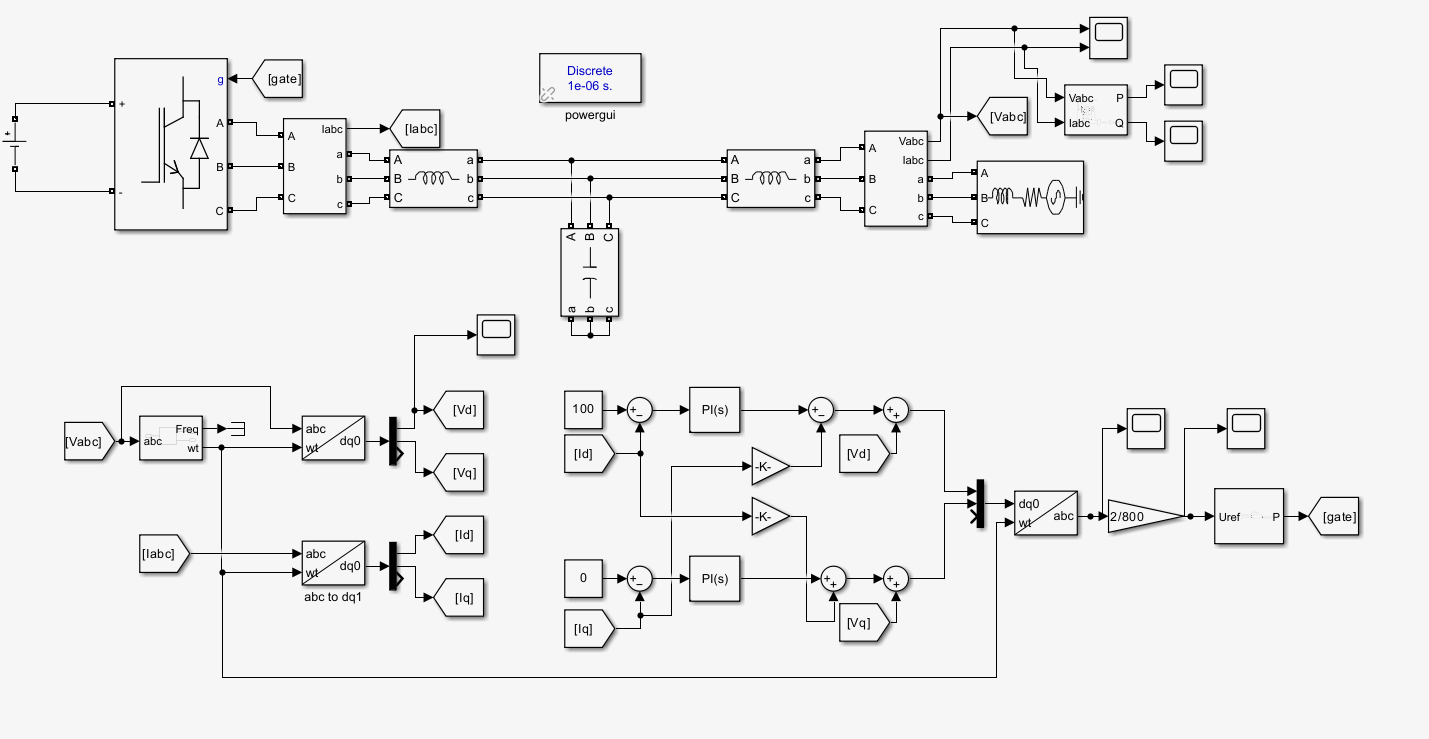
\includegraphics[width=1.1\textwidth]{Figures/5.4.5.png}
    \caption{Inverter tied with grid.}
    \label{inverter tied with grid}
\end{figure}
\subsubsection{Results}
Ma is less than 1
\begin{figure}[H]
    \centering
    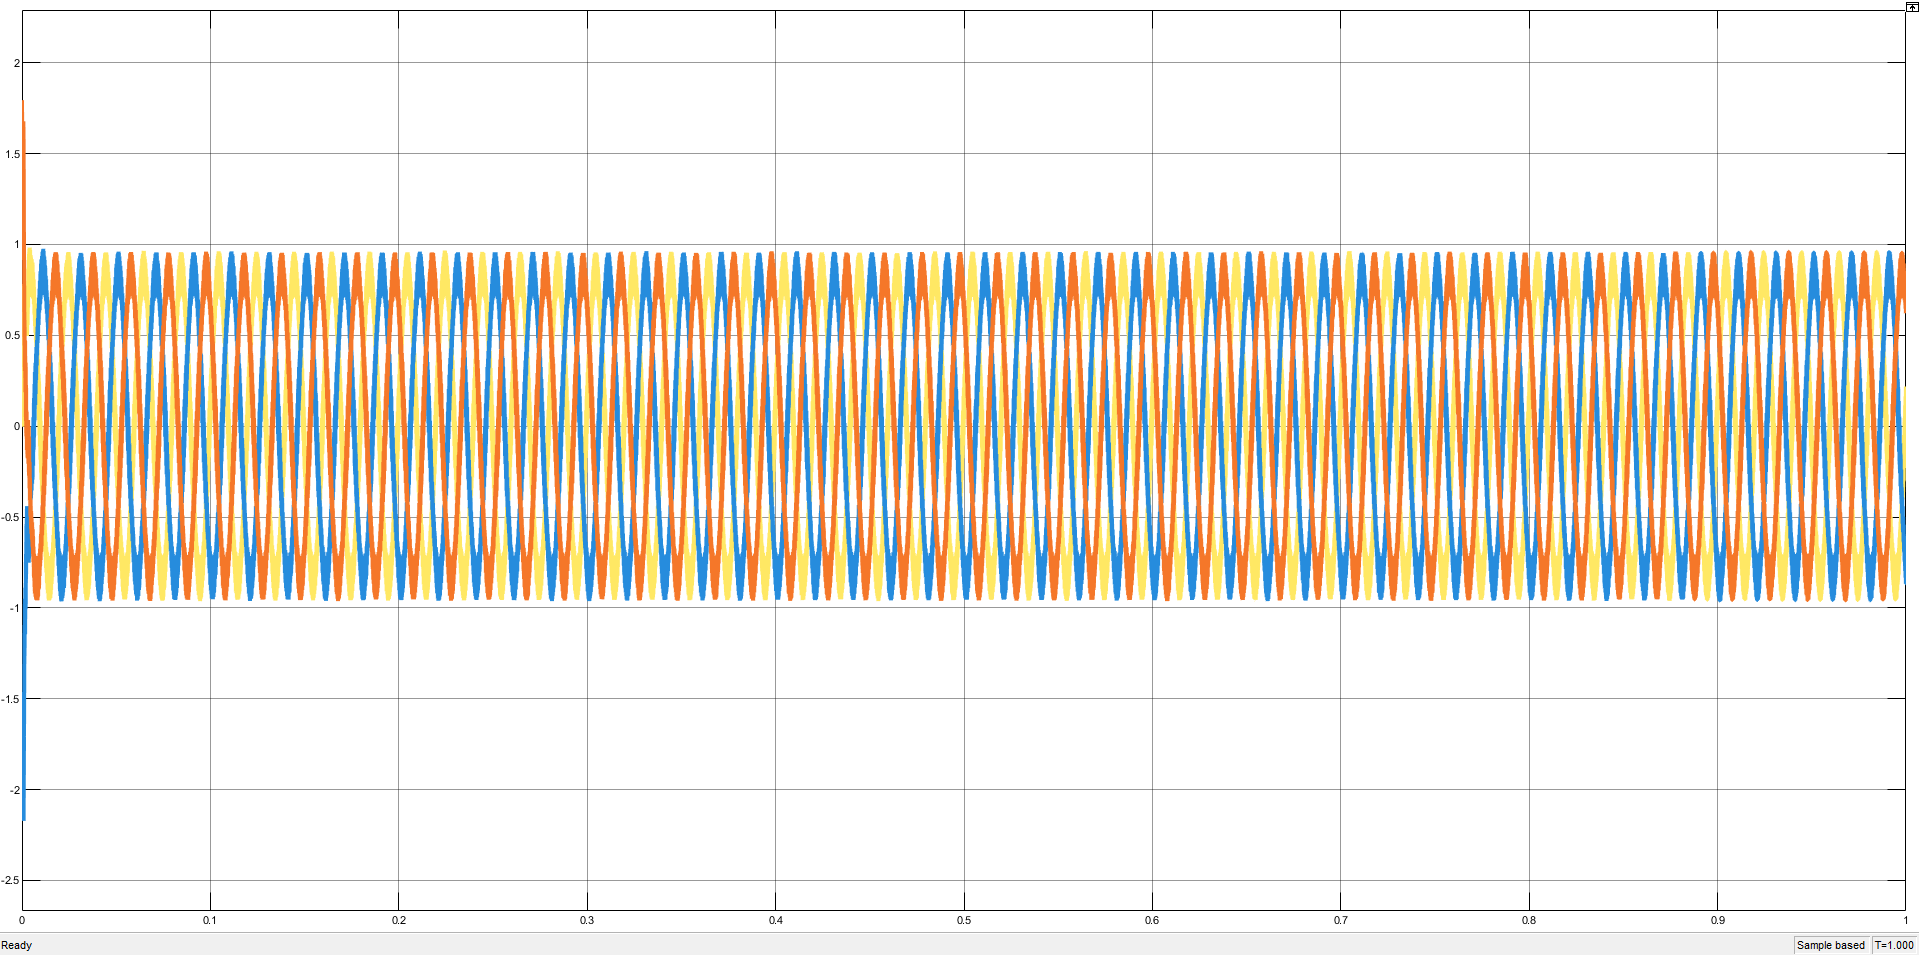
\includegraphics[width=1.1\textwidth]{Figures/5.4.6.png}
    \caption{Modulation index.}
    \label{modulation index}
\end{figure}
\begin{figure}[H]
    \centering
    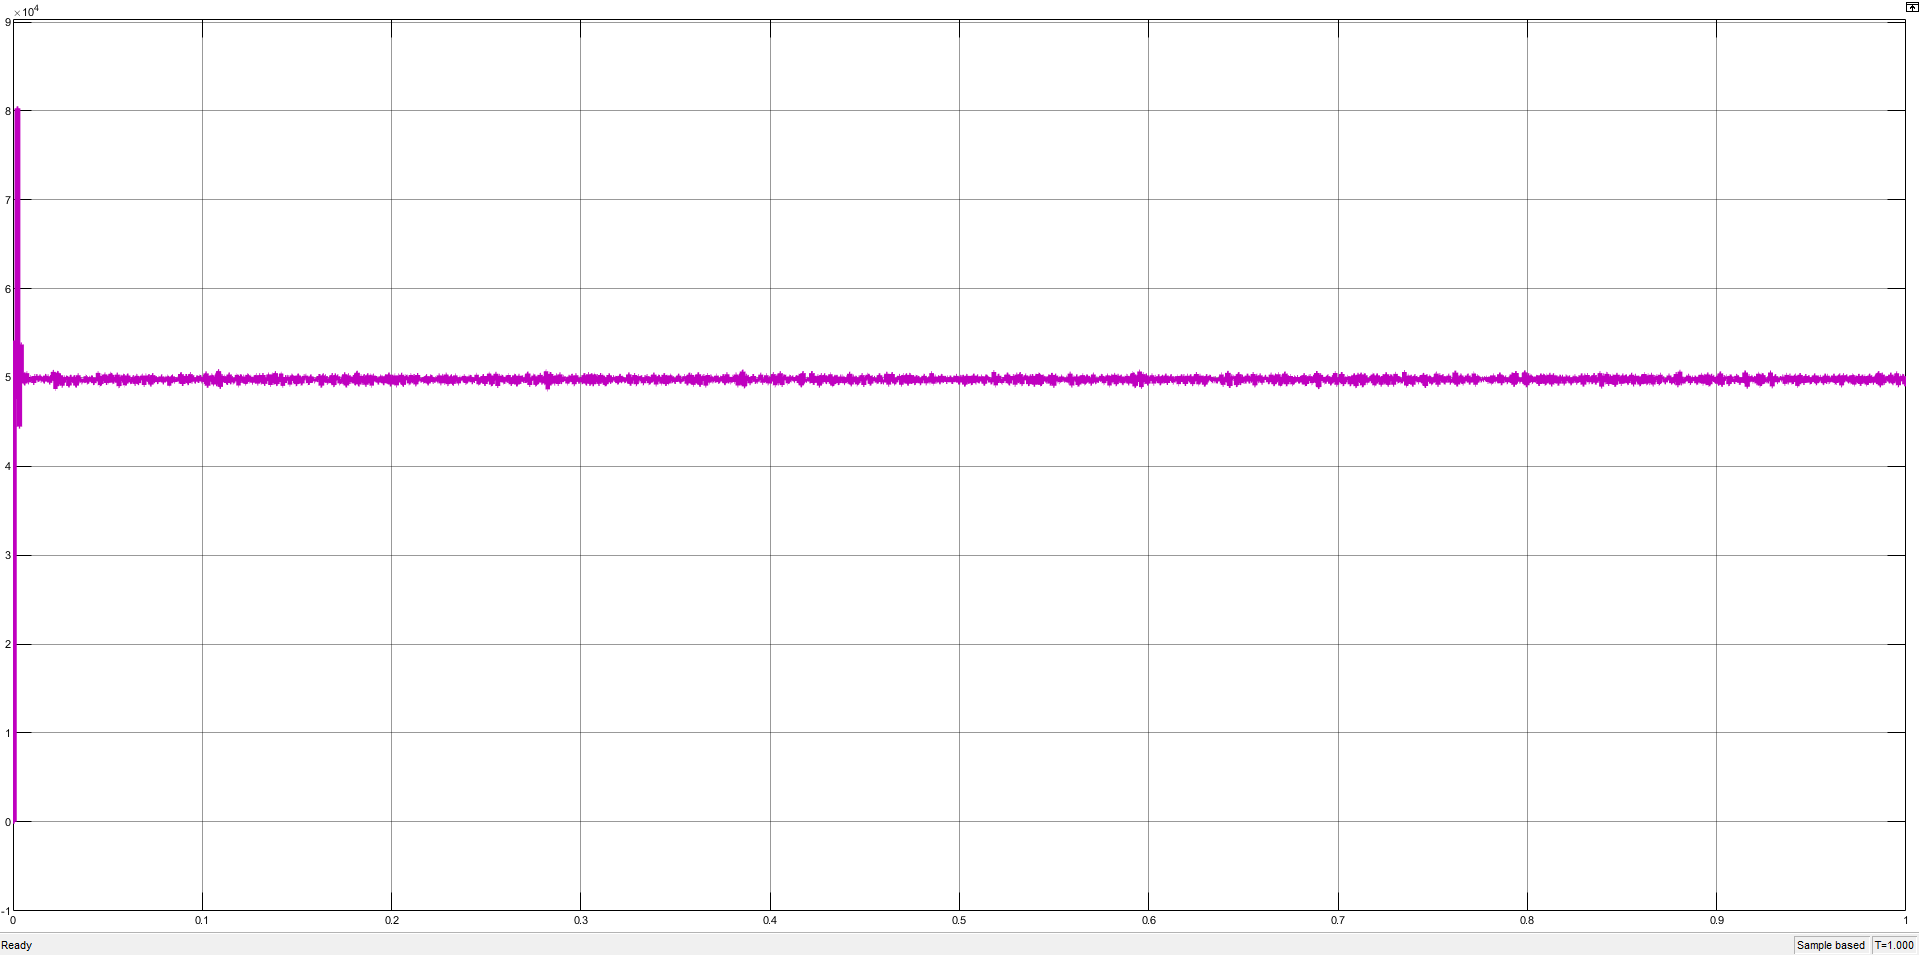
\includegraphics[width=1.1\textwidth]{Figures/5.4.7.png}
    \caption{Grid power.}
    \label{grid power}
\end{figure}

\subsection{Simulation of PV System with Interleaved Boost Tied with Grid}
now the dc link is maintained at 800V as the phase to phase voltage of the grid is 400V
\begin{figure}[H]
    \centering
    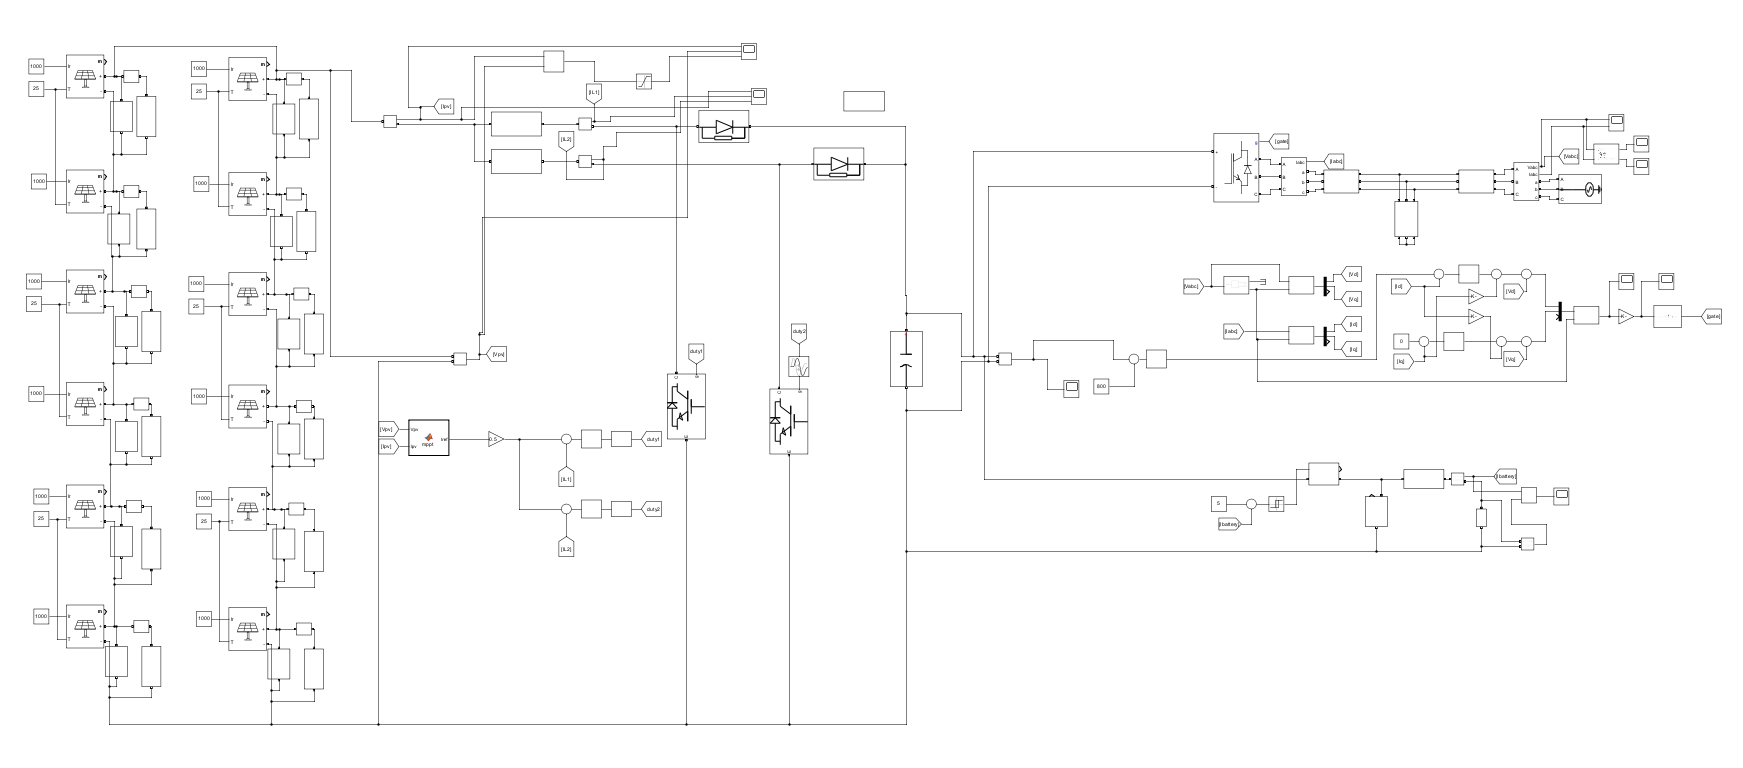
\includegraphics[width=1.1\textwidth]{Figures/5.4.8.png}
    \caption{Grid power.}
    \label{grid power}
\end{figure}

\subsubsection{Results if Ibattery = 10A}
\noindent
\begin{minipage}[t]{0.5\textwidth}
\vspace{0pt}
\begin{itemize}
  \item As shown, current is almost $17.36 \times 2$, the input voltage is also aligned
        with design calculations and output power is 8476\,W, ideally should be 8520\,W,
        but there are switching losses and conduction losses (diodes have forward voltage,
        etc.).

  \item now the dc link is maintained at 800V as the phase to phase voltage of the grid is 400V

  \item Ripples of inductor current $= 35.38 - 34.78 = 0.6$\,A.
  \item as Ibattery = 10A so dc link will send the rest power to the grid.
\end{itemize}
\end{minipage}
\hfill
\begin{minipage}[t]{0.4\textwidth}
\vspace{0pt}
  \centering
  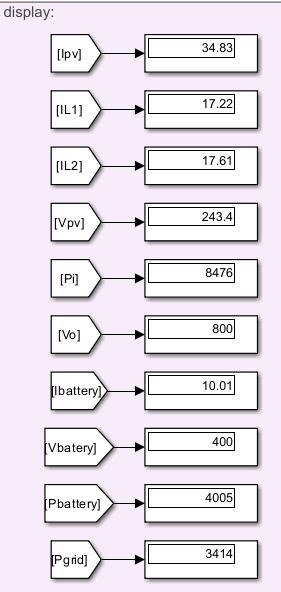
\includegraphics[width=\textwidth]{Figures/5.4.9.png}
  \captionof{figure}{Displays of System.}
  \label{fig:Displays of system}
\end{minipage}

\begin{figure}[H]
    \centering
    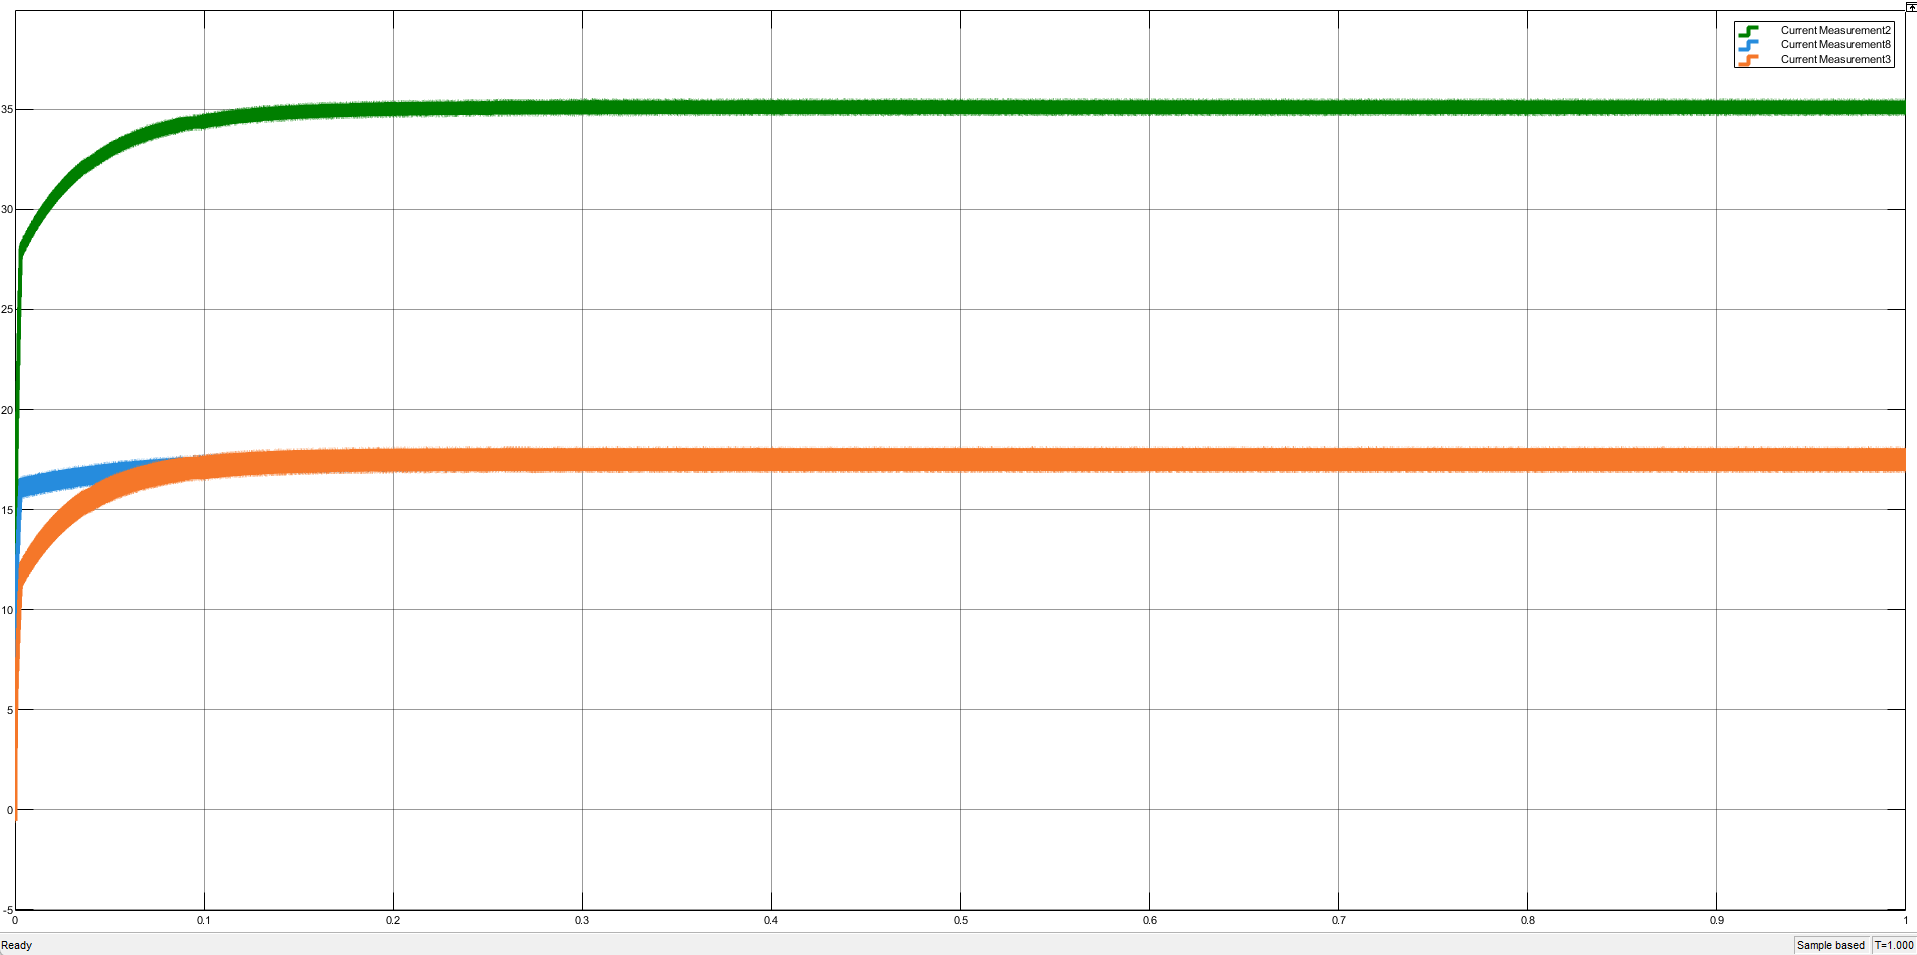
\includegraphics[width=1\textwidth]{Figures/5.4.10.png}
    \caption{Total Current, Inductor Current 1, Inductor Current 2.}
    \label{total current , inductor current 1 ,  inductor current 2 of all system}
\end{figure}

\begin{figure}[H]
    \centering
    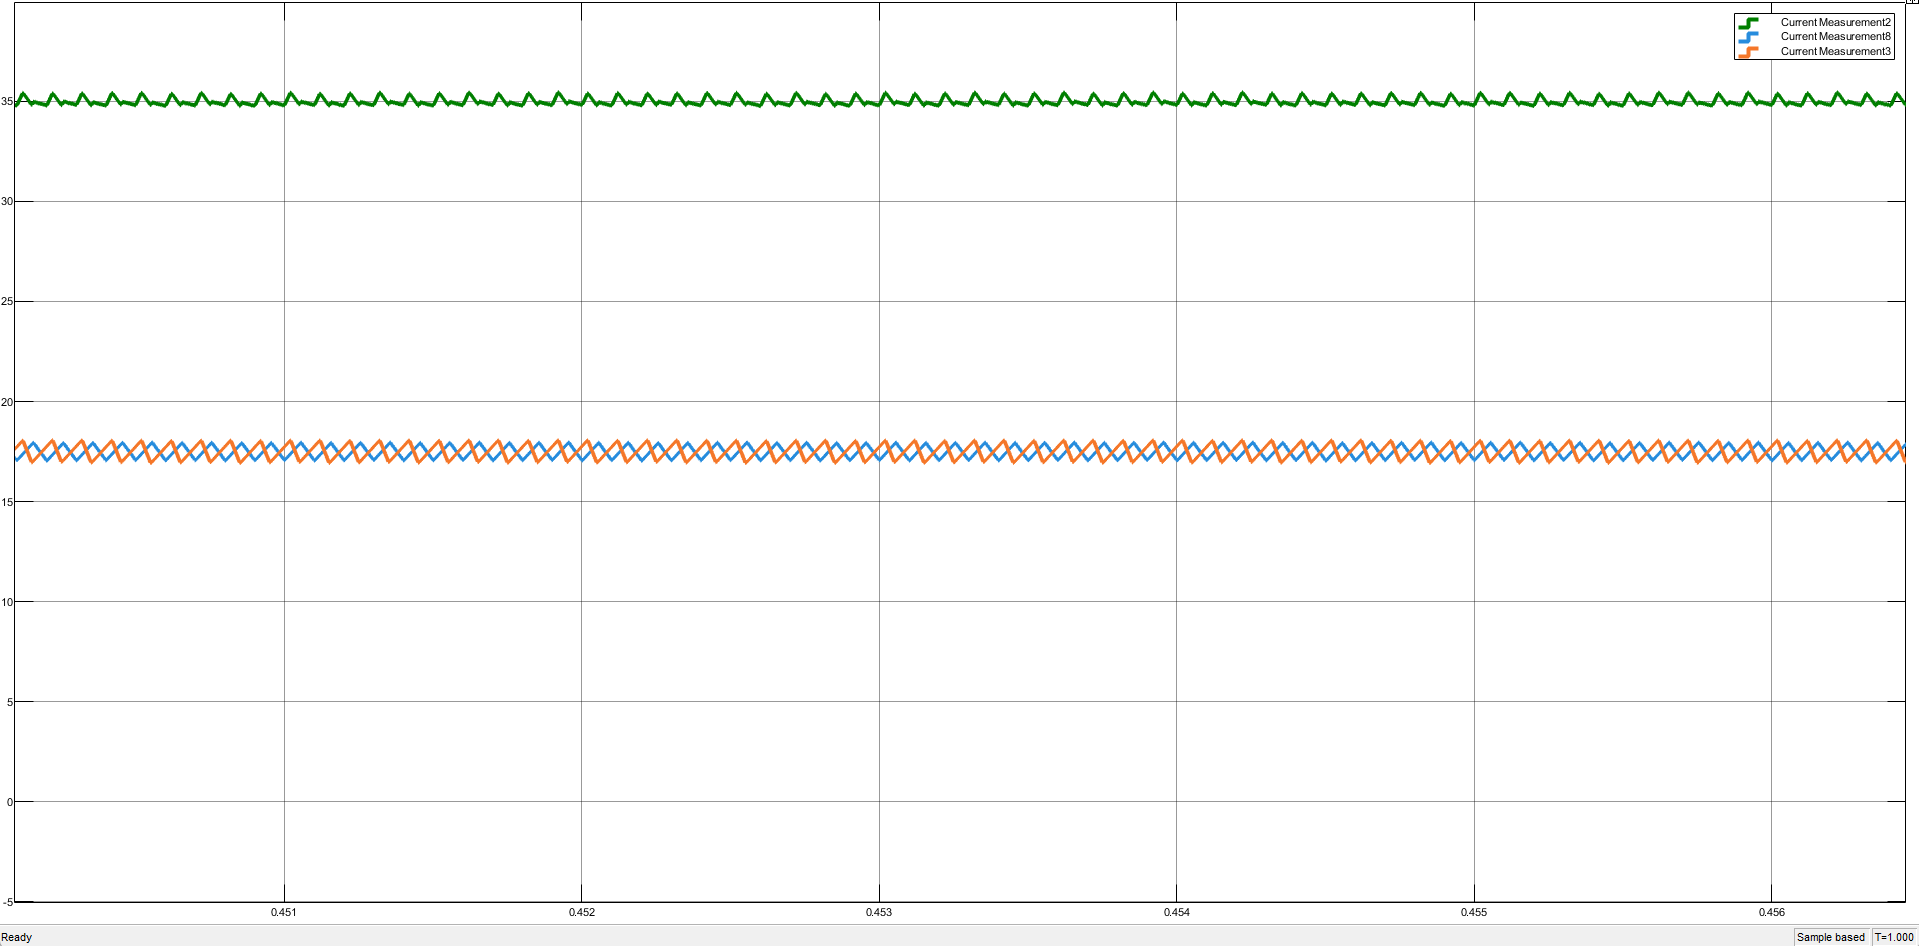
\includegraphics[width=1\textwidth]{Figures/5.4.11.png}
    \caption{Total Current, Inductor Current 1, Inductor Current 2.}
    \label{total current , inductor current 1 ,  inductor current 2 zoom of all system}
\end{figure}

\begin{figure}[H]
    \centering
    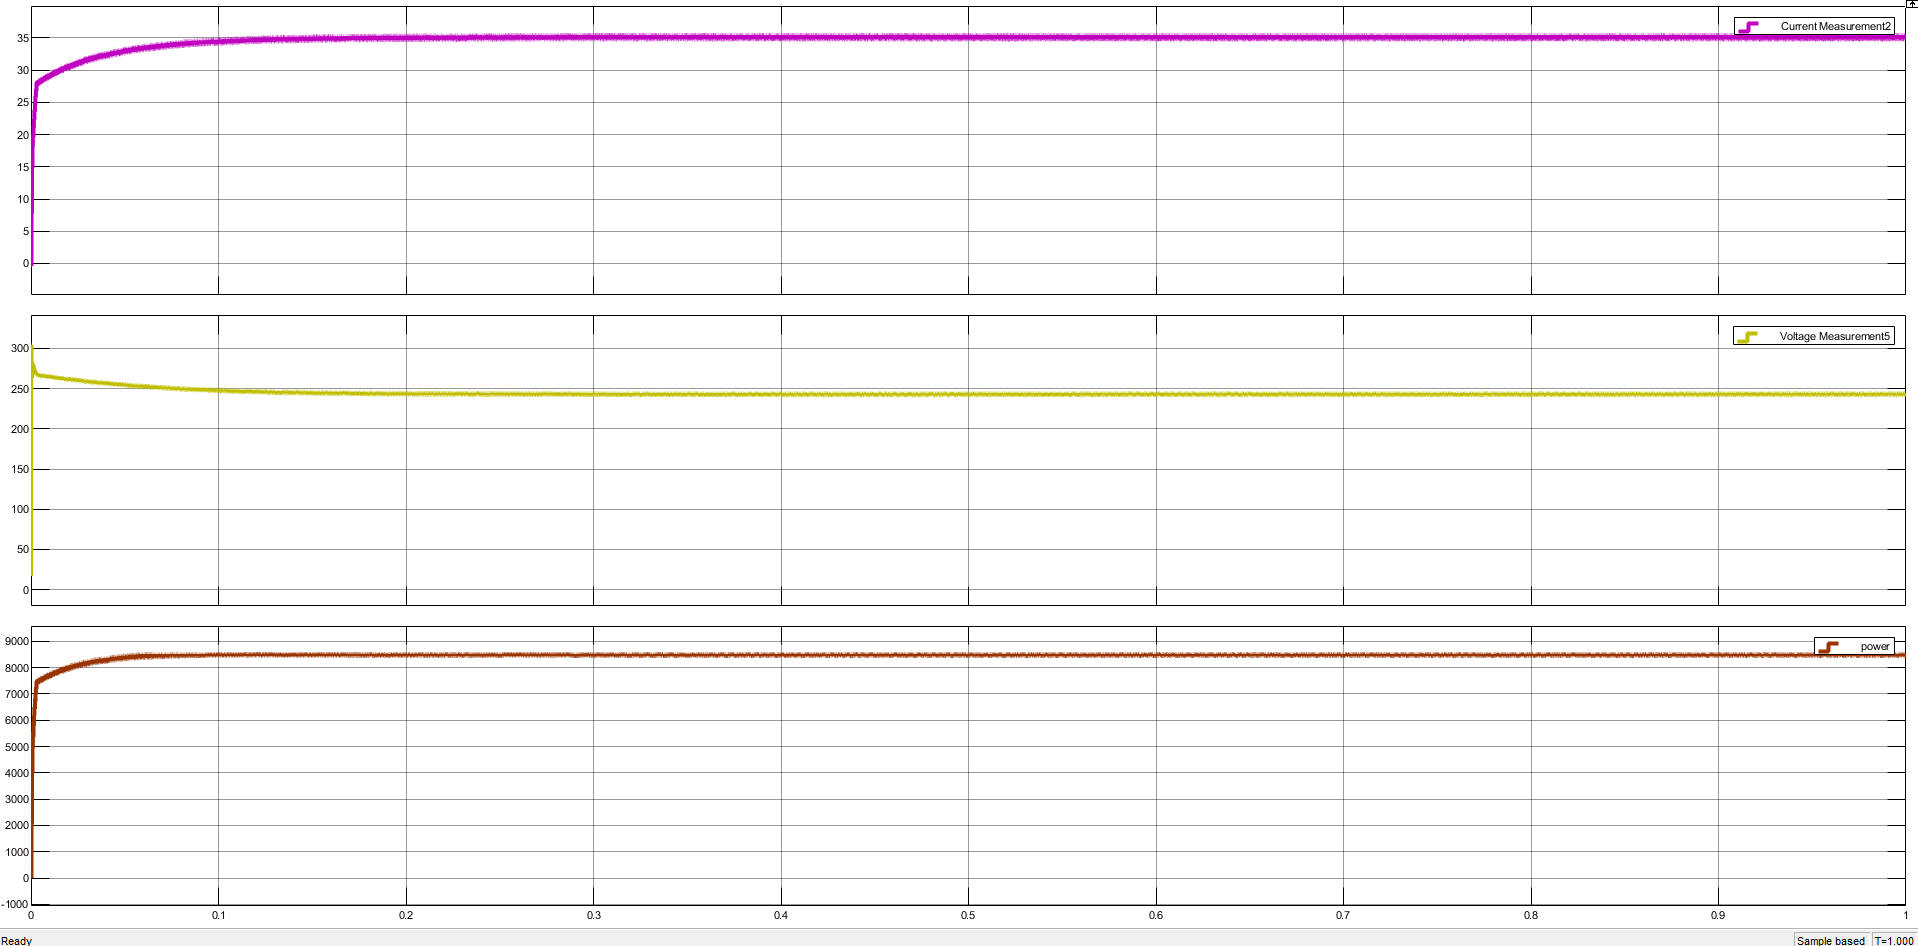
\includegraphics[width=1\textwidth]{Figures/5.4.12.png}
    \caption{Input Current, Voltage, Power.}
    \label{input current , voltage , power. of all system}
\end{figure}

\begin{figure}[H]
    \centering
    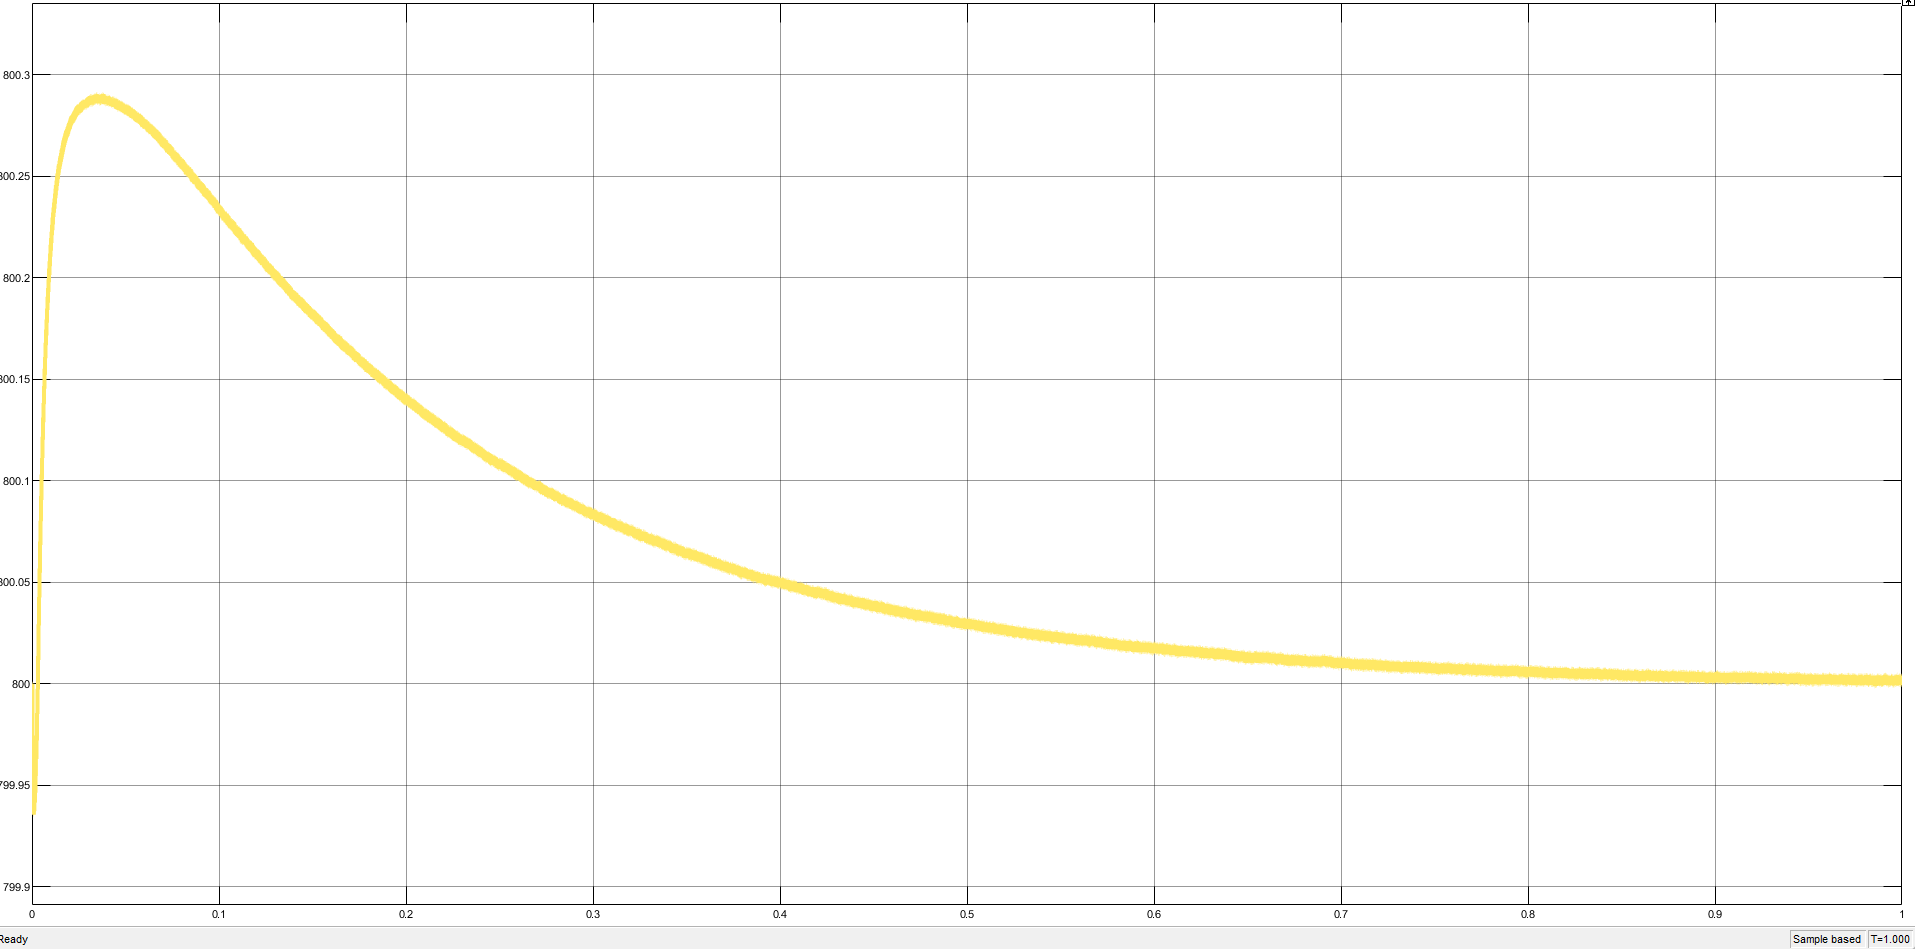
\includegraphics[width=1\textwidth]{Figures/5.4.13.png}
    \caption{Output Voltage.}
    \label{Output voltage of all system}
\end{figure}

\begin{figure}[H]
    \centering
    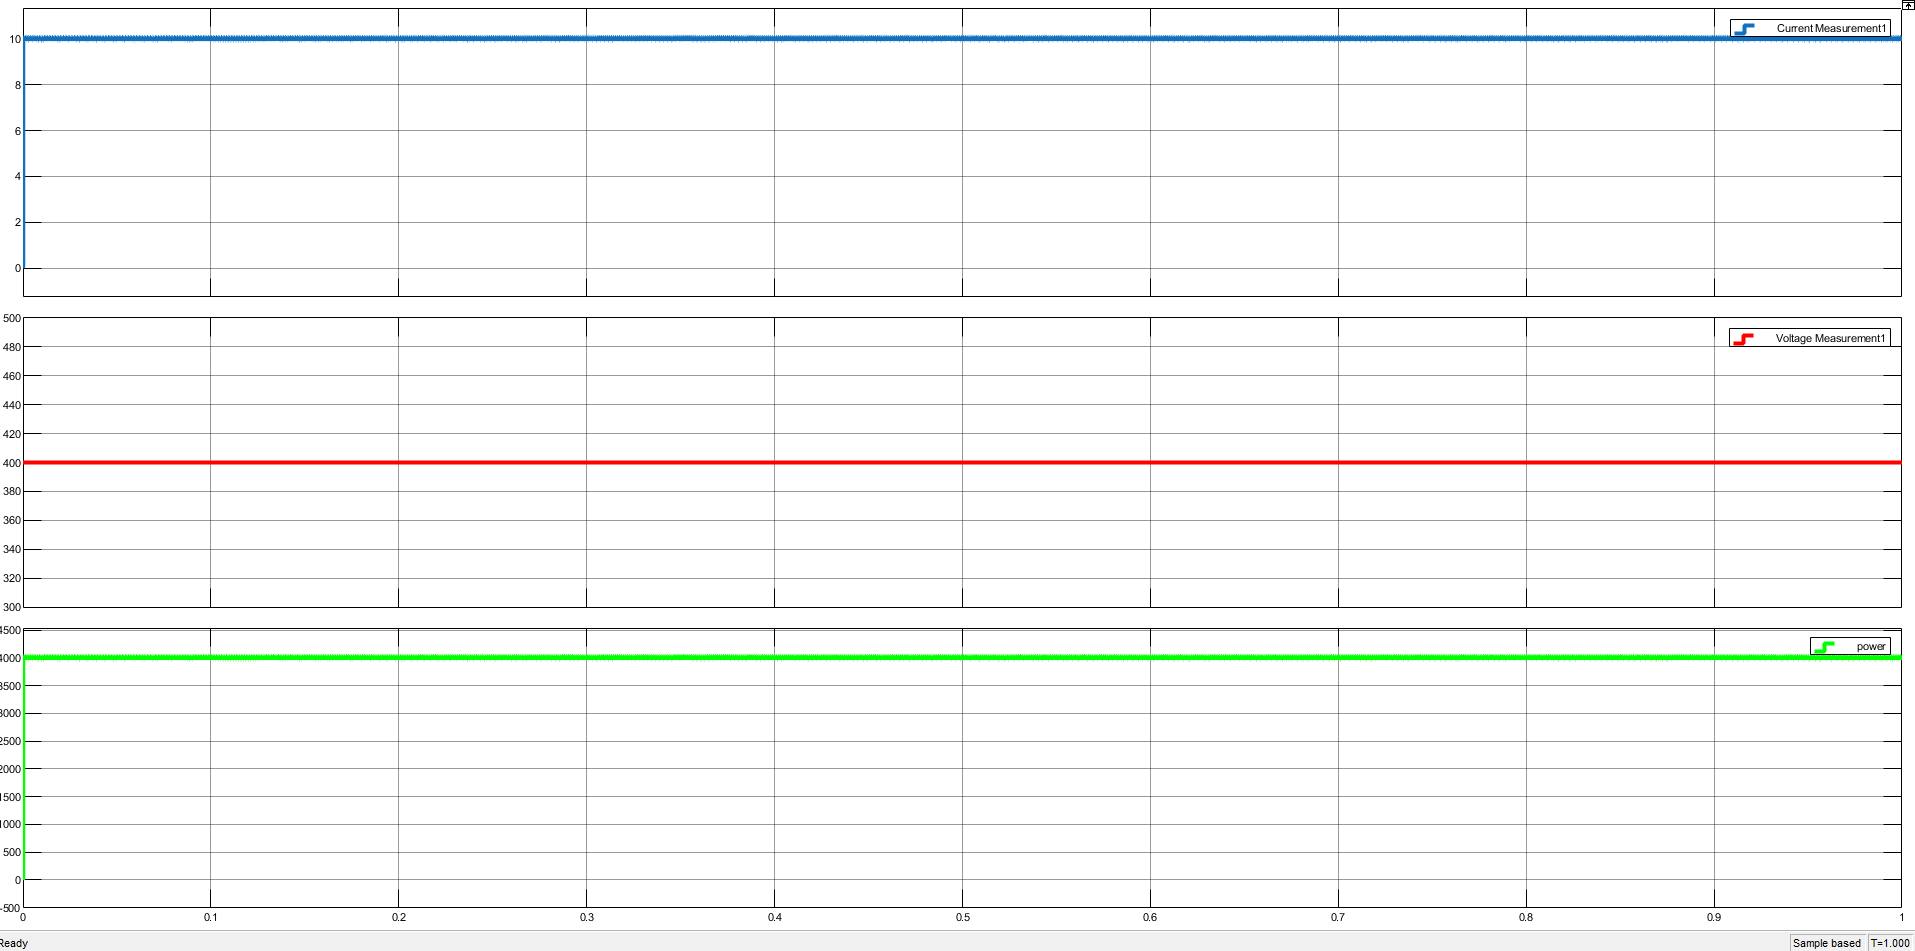
\includegraphics[width=1\textwidth]{Figures/5.4.14.png}
    \caption{Ibattery, Vbattery, Pbattery.}
    \label{Ibattery , Vbattery , Pbattery of all system}
\end{figure}

\begin{figure}[H]
    \centering
    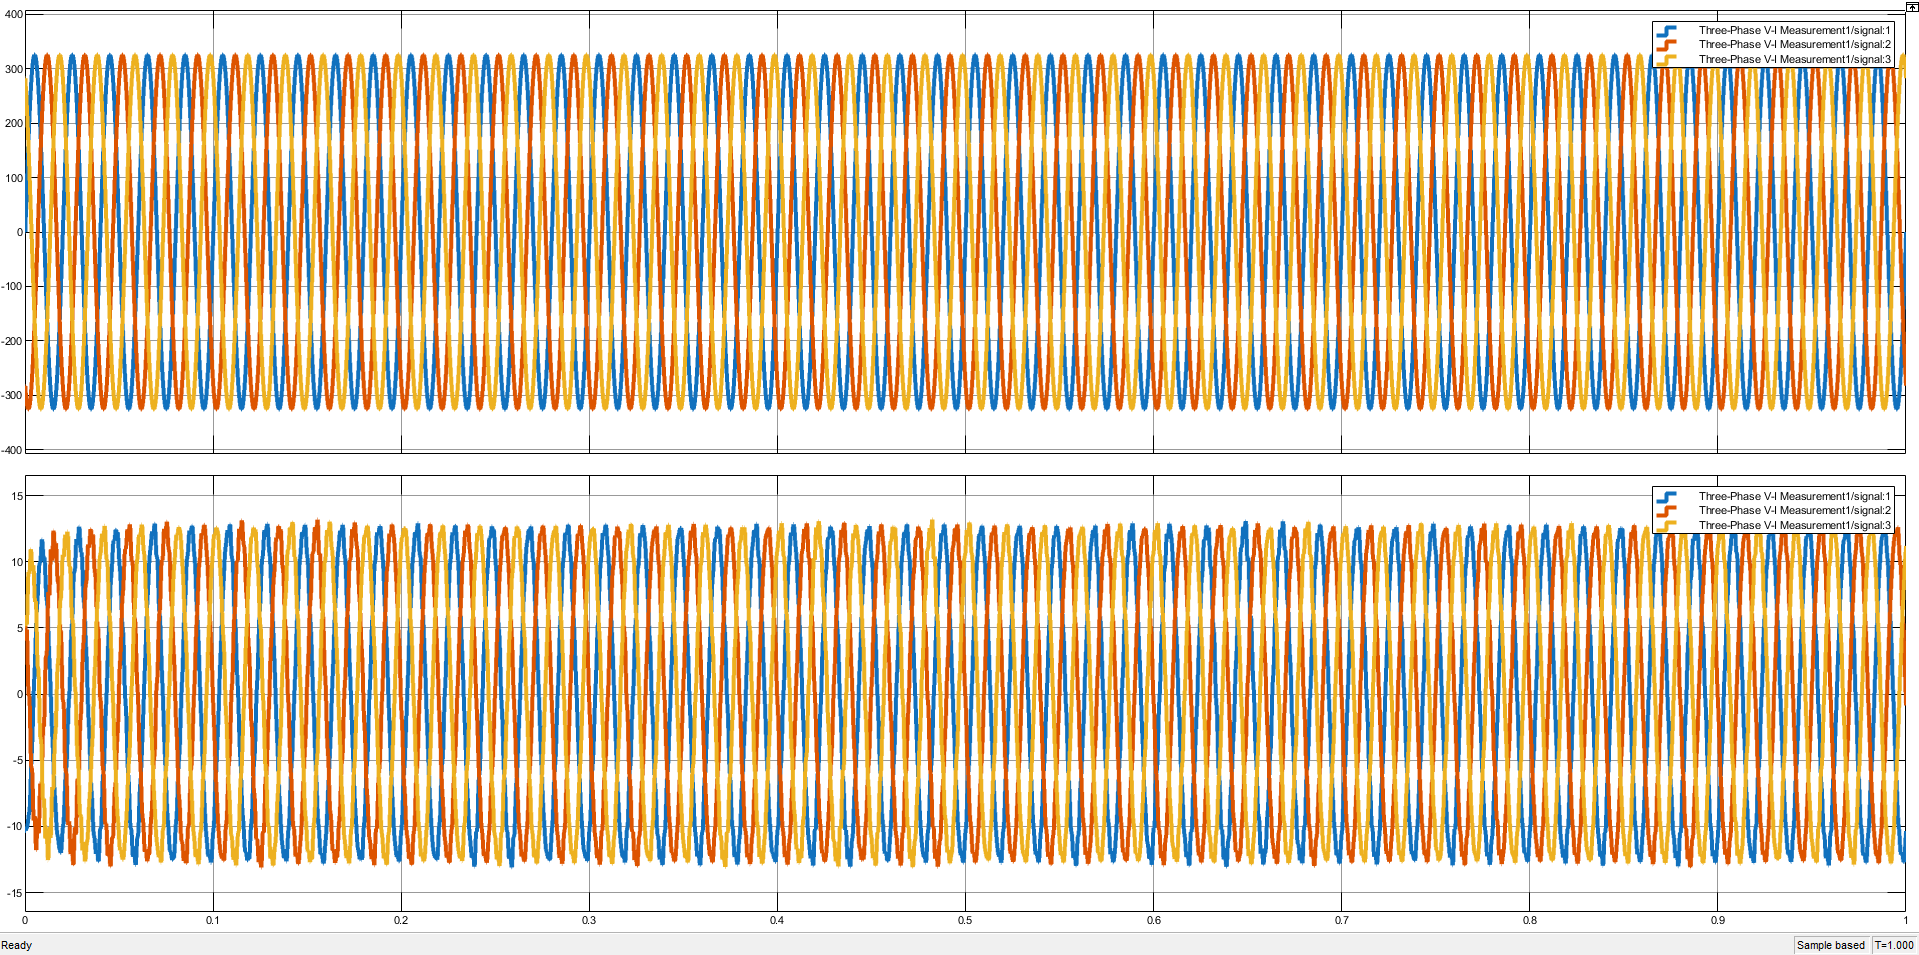
\includegraphics[width=1\textwidth]{Figures/5.4.15.png}
    \caption{3-phase Voltage, 3-phase Current.}
    \label{3-phase voltage , 3-phase current}
\end{figure}

\begin{figure}[H]
    \centering
    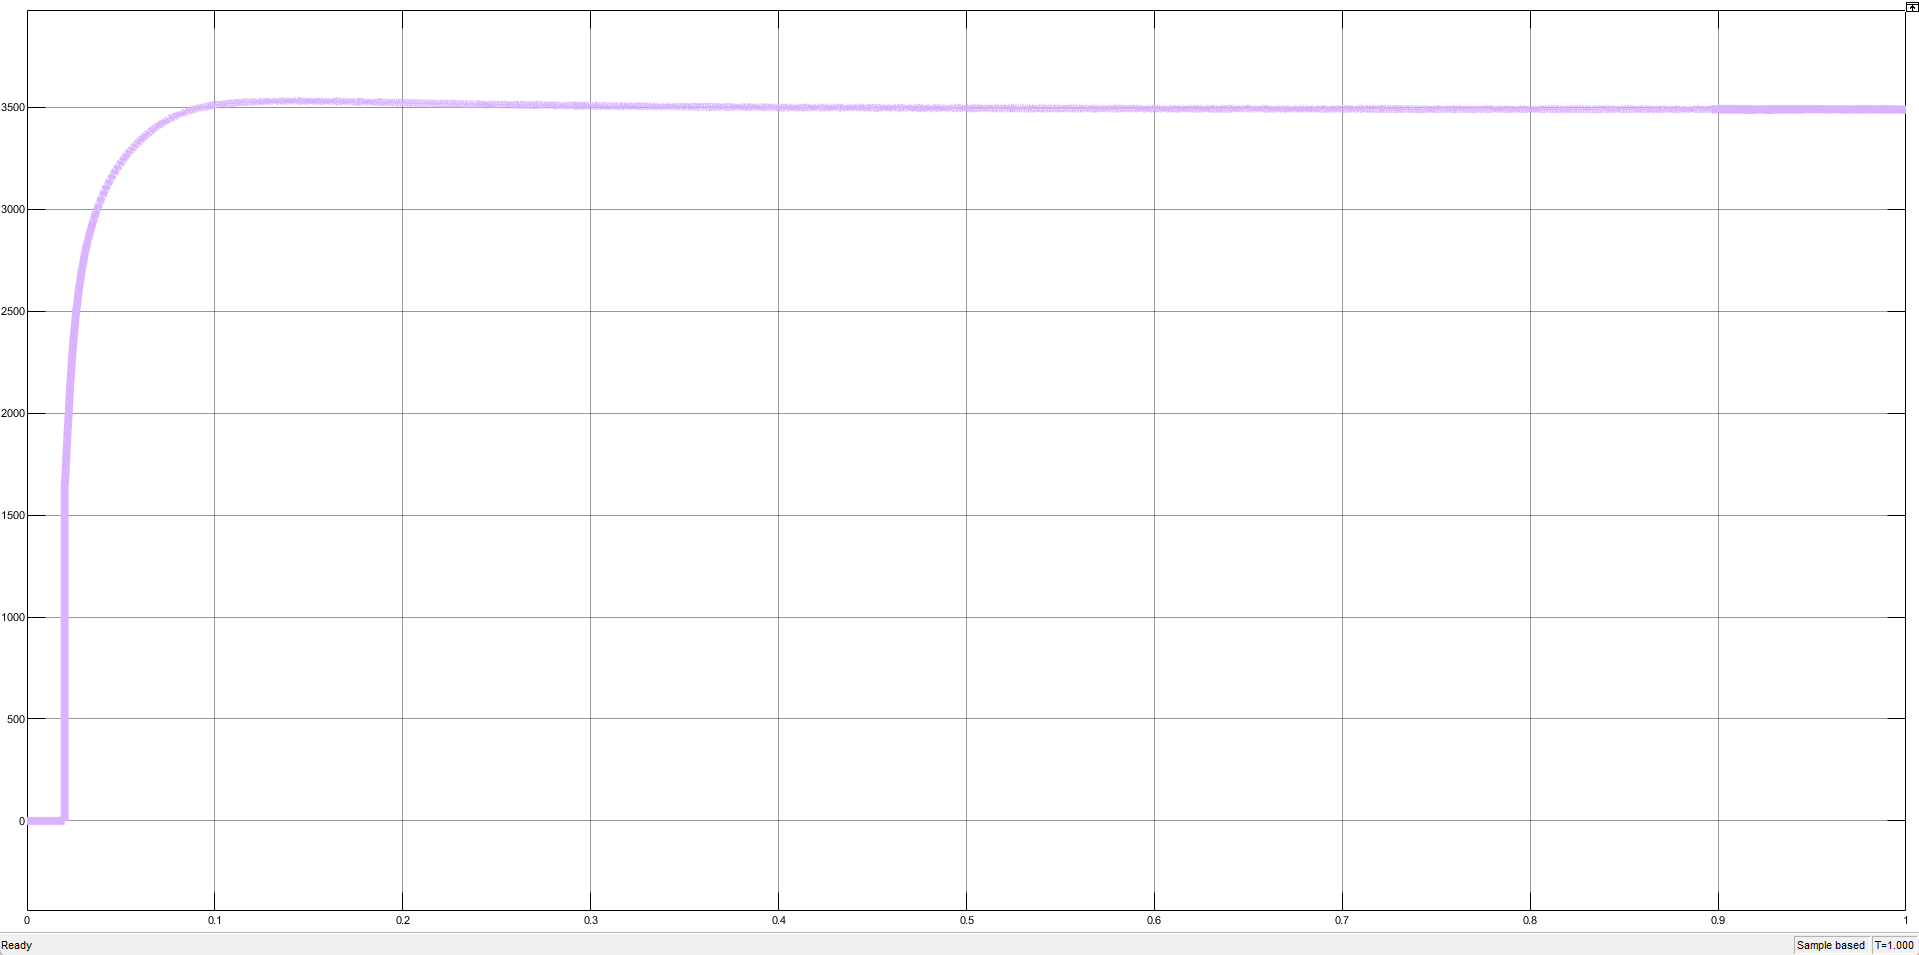
\includegraphics[width=1\textwidth]{Figures/5.4.16.png}
    \caption{Grid Power.}
    \label{grid power oa the system}
\end{figure}

\subsubsection{Results if Ibattery = 30A}
\noindent
\begin{minipage}[t]{0.5\textwidth}
\vspace{0pt}
\begin{itemize}
  \item As shown, current is almost $17.36 \times 2$, the input voltage is also aligned
        with design calculations and output power is 8492\,W, ideally should be 8520\,W,
        but there are switching losses and conduction losses (diodes have forward voltage,
        etc.).

  \item now the dc link is maintained at 800V as the phase to phase voltage of the grid is 400V

  \item Ripples of inductor current $= 35.38 - 34.78 = 0.6$\,A.
  \item as Ibattery = 30A so dc link will Receive the rest power from the grid so EV can be fully chargred.
   \item the rest graphs will be the same as case 1.
\end{itemize}
\end{minipage}
\hfill
\begin{minipage}[t]{0.4\textwidth}
\vspace{0pt}
  \centering
  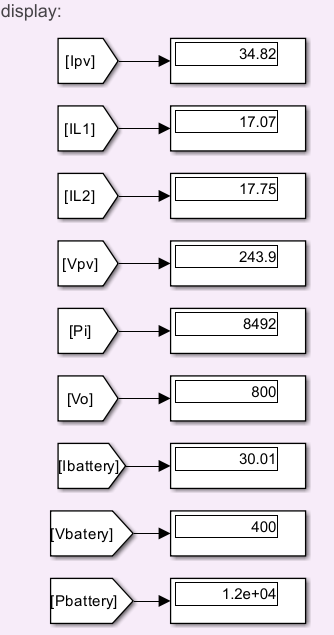
\includegraphics[width=\textwidth]{Figures/5.4.17.png}
  \captionof{figure}{Displays of system.}
  \label{fig:Displays of system2}
\end{minipage}

\begin{figure}[H]
    \centering
    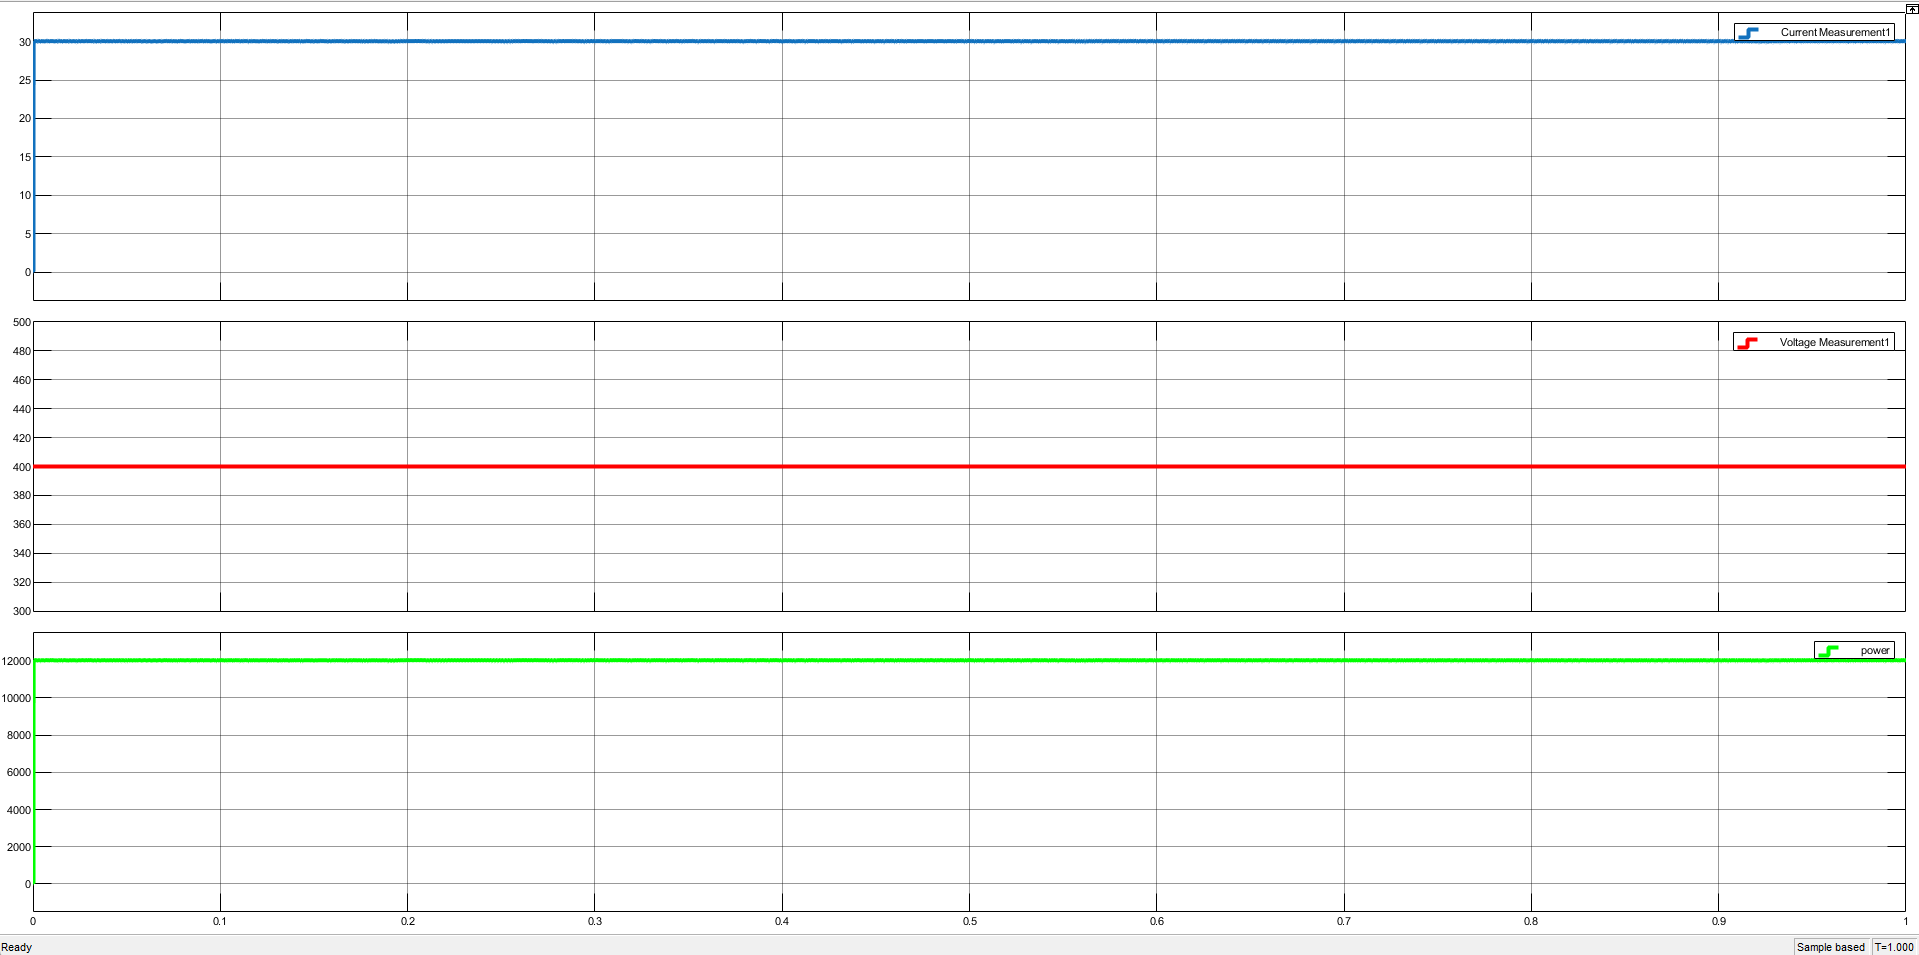
\includegraphics[width=1\textwidth]{Figures/5.4.18.png}
    \caption{Ibattery, Vbattery, Pbattery.}
    \label{Ibattery , Vbattery , Pbattery of all system2}
\end{figure}

\begin{figure}[H]
    \centering
    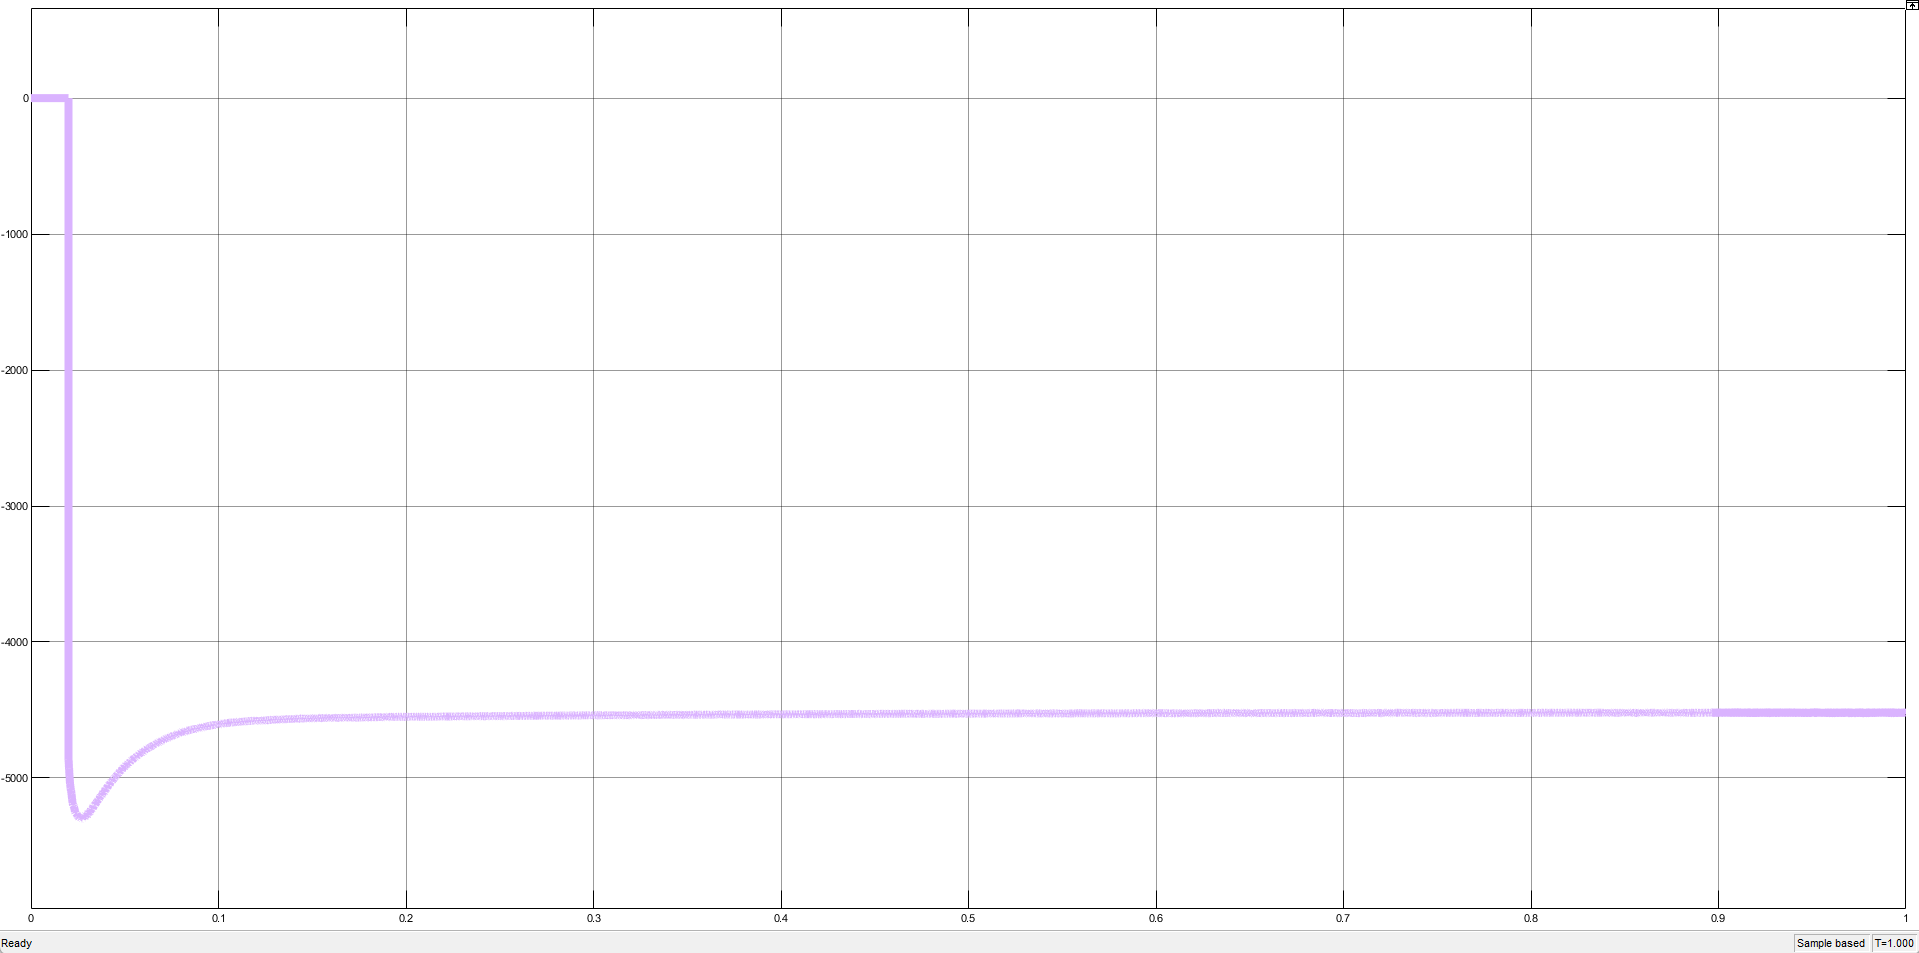
\includegraphics[width=1\textwidth]{Figures/5.4.19.png}
    \caption{Grid Power.}
    \label{grid power of the system2}
\end{figure}

\subsection{Simulation of the Off-Grid System (High Ratings)}

\subsubsection{System Modeling and Converter Design}

\begin{figure}[H]
    \centering
    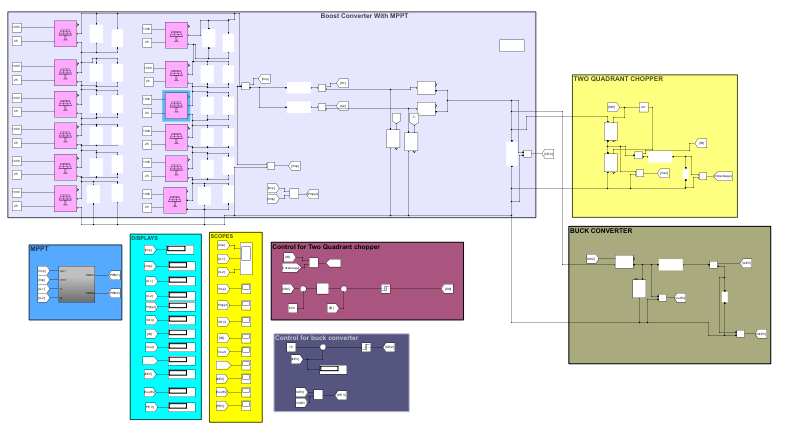
\includegraphics[width=0.9\textwidth]{Figures/full.png}
    \caption{Full System}
    \label{fig:full_system}
\end{figure}

\paragraph{PV Array Specifications}

The photovoltaic (PV) system serves as the primary power source for the overall system. The PV array is designed using a centralized topology to minimize complexity and cost. It consists of six individual PV modules connected in series to form a single string, while two strings are connected in parallel. Based on the specifications of a single PV module, the overall array characteristics under Standard Test Conditions (STC: 1000~W/m$^{2}$, 25$^\circ$C) are calculated as follows.

\begin{align}
V_{MPP} &= 6 \times 40.9 = 245.4~\text{V}
\end{align}

\begin{align}
I_{MPP} &= 2 \times 17.36 = 34.72~\text{A}
\end{align}

\begin{align}
V_{OC} &= 294~\text{V}
\end{align}

\begin{align}
I_{SC} &= 2 \times 18.4 = 36.8~\text{A}
\end{align}

\begin{align}
P_{MAX} &= 245.4 \times 34.72 = 8520~\text{W}
\end{align}

\begin{table}[H]
\centering
\caption{PV Array Specifications}
\label{tab:pv_specifications}
\begin{tabular}{|l|c|}
\hline
\textbf{Parameter} & \textbf{Value} \\
\hline
Voltage at Maximum Power ($V_{MPP}$) & 245.4 V \\
Current at Maximum Power ($I_{MPP}$) & 34.72 A \\
Open-Circuit Voltage ($V_{OC}$) & 294 V \\
Short-Circuit Current ($I_{SC}$) & 36.8 A \\
Maximum Output Power ($P_{MAX}$) & 8520 W \\
\hline
\end{tabular}
\end{table}

\begin{figure}[H]
    \centering
    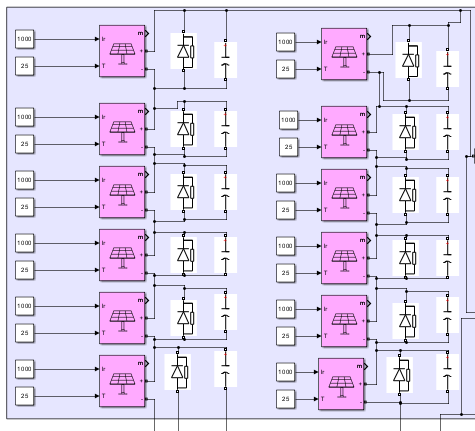
\includegraphics[width=0.8\textwidth]{Figures/pvm.png}
    \caption{PV Modules}
    \label{fig:mpp_current}
\end{figure}
\begin{figure}[H]
    \centering
    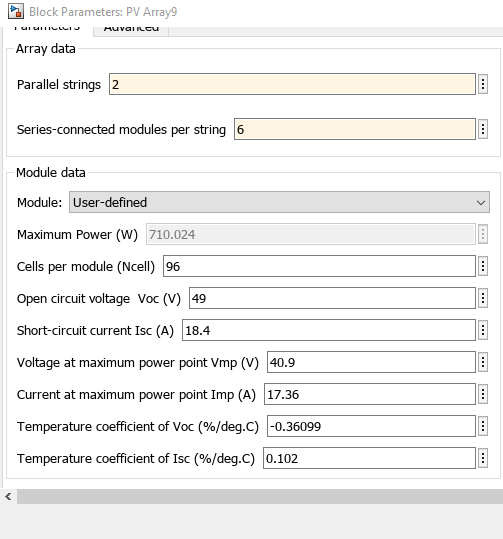
\includegraphics[width=0.8\textwidth]{Figures/rating.png}
    \caption{Rating of One Module}
    \label{fig:mpp_current}
\end{figure}
\begin{figure}[H]
    \centering
    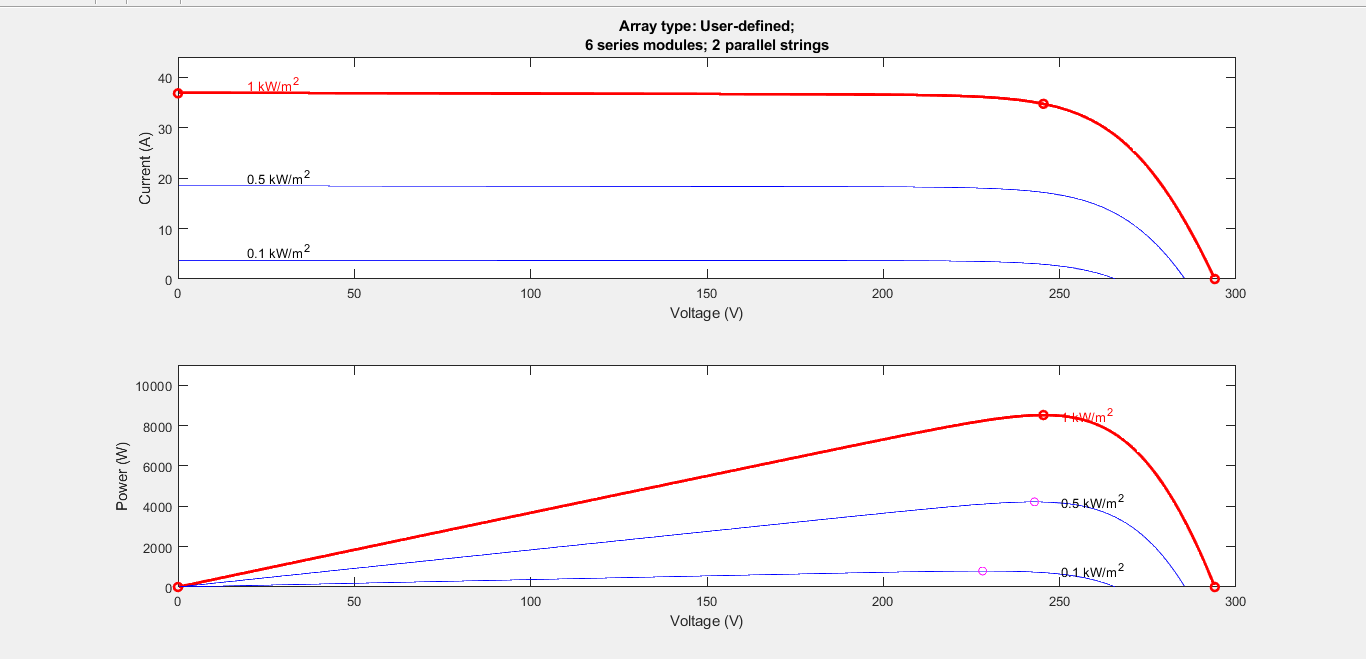
\includegraphics[width=0.8\textwidth]{Figures/mppt2.png}
    \caption{Max Power point }
    \label{fig:mpp_current}
\end{figure}

\subsubsection{Boost Converter and MPPT Operation}

\begin{figure}[H]
    \centering
    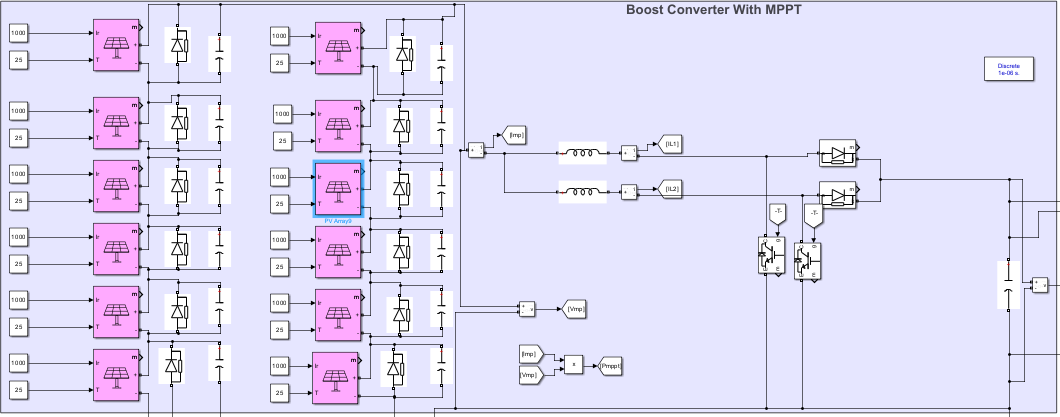
\includegraphics[width=0.8\textwidth]{Figures/boost.png}
    \caption{Boost Converter}
    \label{fig:boost_converter}
\end{figure}

Since the output voltage of the PV array ($245.4~\mathrm{V}$) fluctuates continuously due to variations in solar irradiance and temperature, and is typically lower than the required common DC bus voltage, a DC--DC Boost Converter is integrated. This converter performs two critical functions.

\paragraph{Voltage Stepping-Up}

The converter regulates and steps up the fluctuating PV array voltage to maintain a stable DC bus voltage of $600~\mathrm{V}$. Based on the continuous conduction mode (CCM) equation of the boost converter, the theoretical duty cycle at the maximum power point is calculated as follows:

\begin{equation}
D = 1-\frac{V_{in}}{V_{out}}
\end{equation}

\begin{equation}
D = 1-\frac{245.4}{600}=0.591
\end{equation}

This indicates that the converter operates with a nominal duty cycle of approximately $59.1\%$ under Standard Test Conditions (STC).

\paragraph{Maximum Power Extraction}

The duty cycle of the boost converter is controlled by a Maximum Power Point Tracking (MPPT) algorithm. This ensures that the PV array continuously operates at its optimal voltage and current, extracting the maximum available electrical power of approximately $8520~\mathrm{W}$ despite environmental variations.
\newpage
\subsubsection{Internal Architecture of the MPPT Subsystem}

This subsystem is implemented based on the Perturb and Observe (P\&O) algorithm [5]. The operational mechanism consists of the following stages:

\begin{itemize}

\item \textbf{Power Change ($\Delta P$) Calculation}

The instantaneous PV voltage ($V_{pv1}$) and current ($I_{pv1}$) are measured and multiplied to calculate the output power

\begin{equation}
P=V\times I
\end{equation}

The previous power value is stored using a Unit Delay ($1/z$) block and compared with the current value to calculate the power variation ($\Delta P$).

\item \textbf{Reference Current Generation}

According to the sign of $\Delta P$, the controller increments or decrements the reference current ($I_{ref}$) using a fixed step size of $0.05$. This iterative process continuously drives the operating point toward the maximum power point.

\item \textbf{Dual PI Current Control}

Since an Interleaved Boost Converter is employed, the generated reference current is divided between the two converter phases and compared with the measured inductor currents ($I_1$ and $I_2$). Two independent PI controllers regulate each phase to minimize the steady-state current error.

\item \textbf{Interleaved PWM Signal Generation}

Two PWM signals ($PWM_1$ and $PWM_2$) are generated with an accurate $180^\circ$ phase shift using a Delay block. This interleaving technique ensures balanced current sharing between the converter phases, significantly reducing the input current ripple and decreasing the electrical stress on the switching devices.

\end{itemize}

\begin{figure}[H]
    \centering
    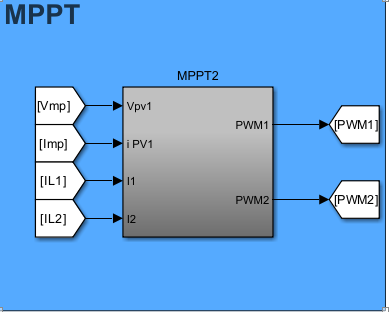
\includegraphics[width=0.8\textwidth]{Figures/mppt block.png}
    \caption{MPPT block}
    \label{fig:mppt_architecture}
\end{figure}
\begin{figure}[H]
    \centering
    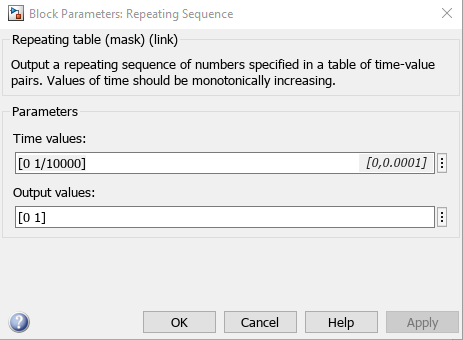
\includegraphics[width=0.8\textwidth]{Figures/repeating sequence.png}
    \caption{Repeating sequence}
    \label{fig:mppt_architecture}
\end{figure}
\begin{figure}[H]
    \centering
    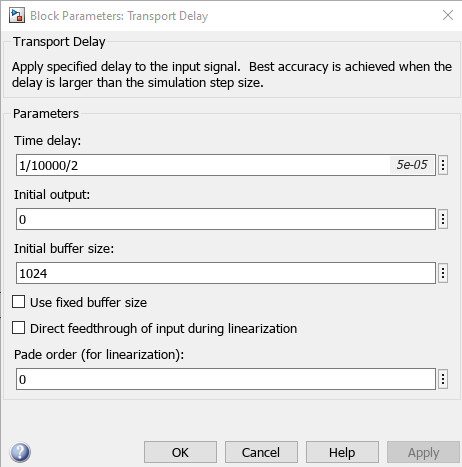
\includegraphics[width=0.8\textwidth]{Figures/transport delay.png}
    \caption{Transport Delay}
    \label{fig:mppt_architecture}
\end{figure}
\begin{figure}[H]
    \centering
    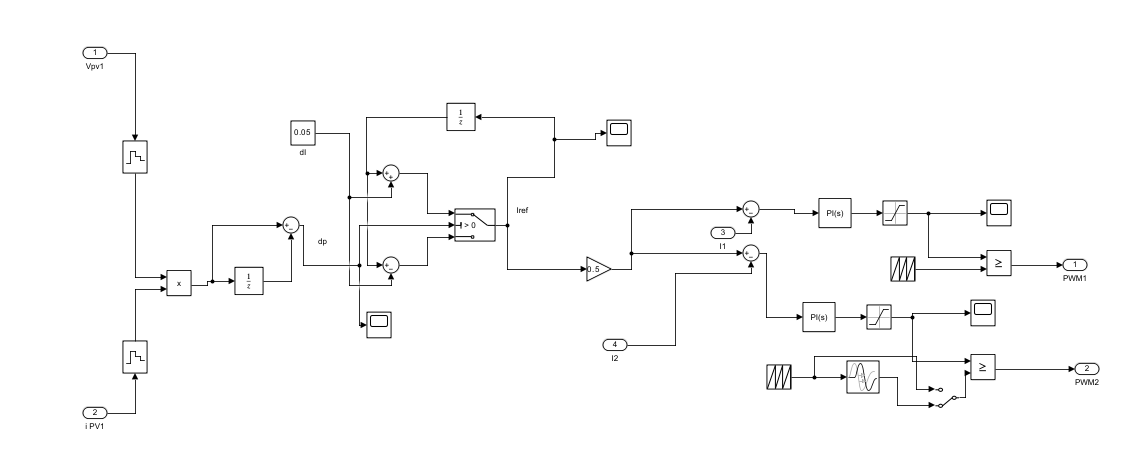
\includegraphics[width=0.8\textwidth]{Figures/intrenal struvture.png}
    \caption{Internal Architecture of the MPPT }
    \label{fig:mppt_architecture}
\end{figure}

\subsubsection{MPPT Using MATLAB Function Block}

To improve power extraction efficiency and reduce the effects of partial shading, a Global Maximum Power Point Tracking (GMPPT) algorithm was implemented using a MATLAB Function block. The algorithm is based on a voltage sweep technique consisting of an outer voltage loop and an inner current control loop.

\paragraph{Voltage Sweep Logic}

The algorithm operates through a finite-state machine with four operating modes:

\begin{itemize}
    \item RESET
    \item SCAN
    \item RETURN
    \item HOLD
\end{itemize}

Initially, the RESET mode drives the PV voltage toward the estimated open-circuit voltage ($250~\mathrm{V}$). During the SCAN mode, the reference voltage is gradually decreased while monitoring the generated power. The algorithm records the global maximum power ($P_{max}$) together with its corresponding voltage ($V_{best}$). The RETURN mode then smoothly drives the operating point back to $V_{best}$, while the HOLD mode maintains this operating point for five seconds before initiating a new sweep cycle.

\paragraph{Inner Current Control Loop}

To force the PV array to accurately track the desired target voltage ($V_{target}$), a digital PI controller with an anti-windup mechanism is implemented. The controller continuously calculates the voltage error and updates the reference current ($I_{ref}$). For safe converter operation, the reference current is limited within the range

\[
0 \le I_{ref} \le 35~\mathrm{A}
\]

which guarantees stable and reliable boost converter performance.

\begin{figure}[H]
    \centering

    \begin{subfigure}[t]{0.4\textwidth}
        \centering
        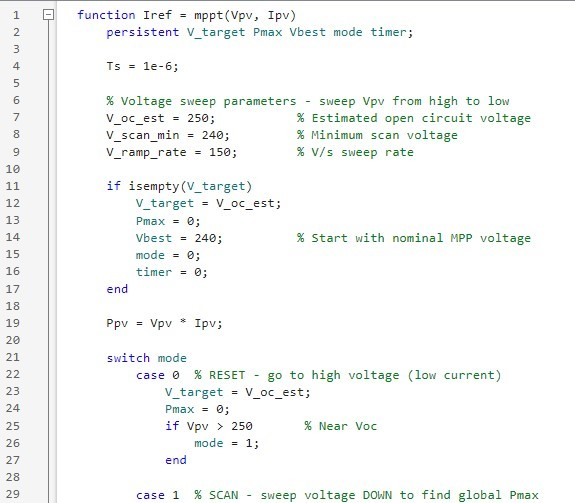
\includegraphics[width=\linewidth]{Figures/mppt1.jpg}
    \end{subfigure}
    \hfill
    \begin{subfigure}[t]{0.4\textwidth}
        \centering
        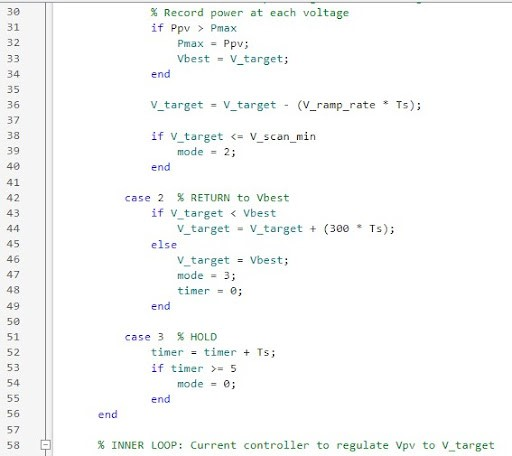
\includegraphics[width=\linewidth]{Figures/mppt2.jpg}
    \end{subfigure}
    \hfill
    \begin{subfigure}[t]{0.4\textwidth}
        \centering
        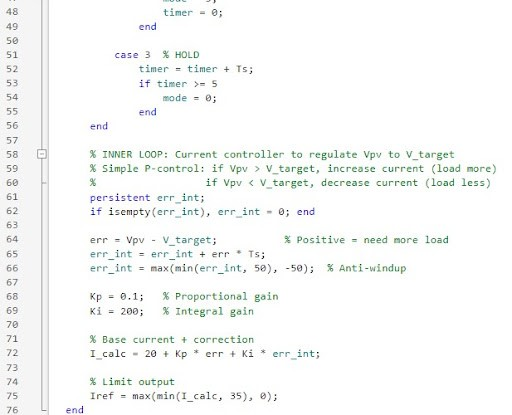
\includegraphics[width=\linewidth]{Figures/mppt3.jpg}
    \end{subfigure}

    \caption{MATLAB implementation of the Global Maximum Power Point Tracking (GMPPT) algorithm using the voltage sweep technique.}
    \label{fig:gmppt_code}
\end{figure}

\subsubsection{Two-Quadrant Chopper}

\paragraph{Primary Function and Operation Modes}

The primary purpose of this circuit is to manage the power flow between the common DC bus and the energy storage system (battery). The converter allows bidirectional power transfer, enabling battery charging from the DC bus in \textbf{Buck mode} and battery discharging to the DC bus in \textbf{Boost mode}.

\begin{figure}[H]
    \centering
    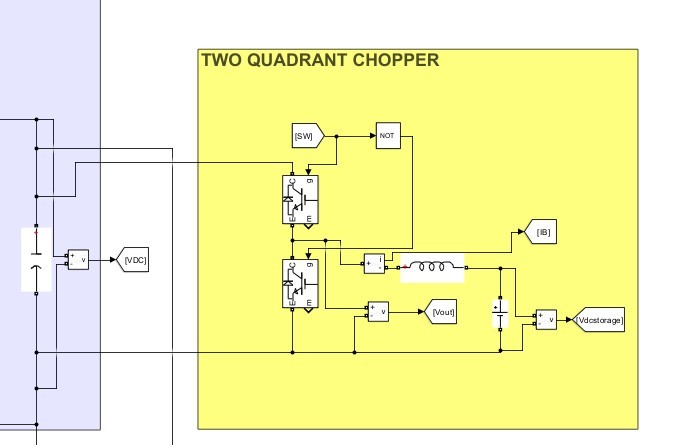
\includegraphics[width=0.7\textwidth]{Figures/2q.jpg}
    \caption{Two-Quadrant Chopper}
    \label{fig:two_quadrant}
\end{figure}

\paragraph{Control Strategy}

The converter employs a closed-loop current control strategy to ensure accurate charging and discharging of the battery. The actual battery current is continuously measured and compared with the reference current. The resulting error is processed by the controller to generate the switching signal.

The generated PWM signal is applied directly to the gate of the first switch, while the complementary signal is obtained through a logical \textbf{NOT} gate and applied to the second switch. This complementary switching guarantees safe converter operation and prevents a short circuit across the DC bus.

\begin{figure}[H]
    \centering
    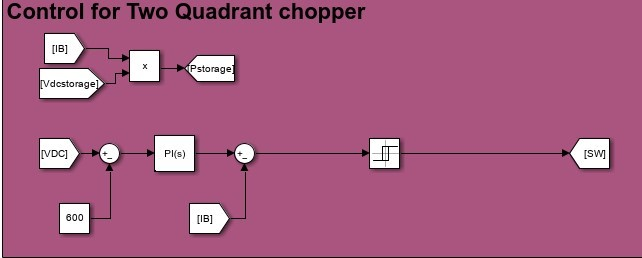
\includegraphics[width=0.7\textwidth]{Figures/2q control.jpg}
    \caption{Control of the Two-Quadrant Chopper}
    \label{fig:two_quadrant_control}
\end{figure}

%%%%%%%%%%%%%%%%%%%%%%%%%%%%%%%%%%%%%%%%%%%%%%%%%%%%%%%%%%%

\subsubsection{DC Buck Converter}

\paragraph{Primary Function}

The DC Buck Converter serves as the final power stage of the system. Its primary function is to step down the common DC bus voltage to a lower regulated voltage suitable for charging the Electric Vehicle (EV) battery. The converter delivers a constant charging current to ensure safe and reliable battery charging.

\begin{figure}[H]
    \centering
    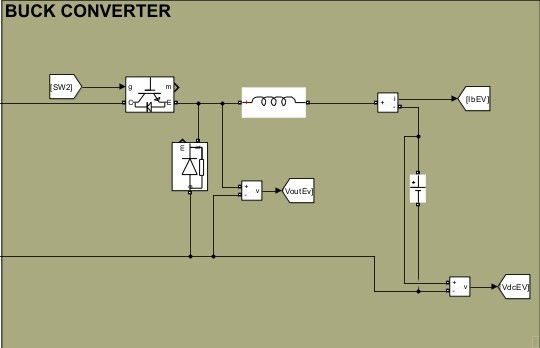
\includegraphics[width=0.8\textwidth]{Figures/buck.jpg}
    \caption{DC Buck Converter}
    \label{fig:buck_converter}
\end{figure}

\paragraph{Control Strategy}

The buck converter employs a closed-loop control system based on the Hysteresis Current Control technique, which is characterized by its fast dynamic response and high current regulation accuracy.

The control strategy consists of the following stages:

\begin{itemize}
    \item \textbf{Current Loop:} A constant reference current of $10~\mathrm{A}$ is defined and continuously compared with the measured EV battery current ($I_{bEV}$).

    \item \textbf{Pulse Generation:} The current error is applied to a Relay block acting as a hysteresis controller. The Relay generates the switching pulses ($SW_2$), forcing the output current to remain within a narrow hysteresis band around the 10 A reference.

    \item \textbf{Power Calculation:} An additional subsystem calculates the instantaneous EV charging power ($P_{EV}$) by multiplying the measured output voltage ($V_{dcEV}$) by the measured battery current ($I_{bEV}$):

    \begin{equation}
    P_{EV}=V_{dcEV}\times I_{bEV}
    \end{equation}

    \begin{figure}[H]
    \centering
    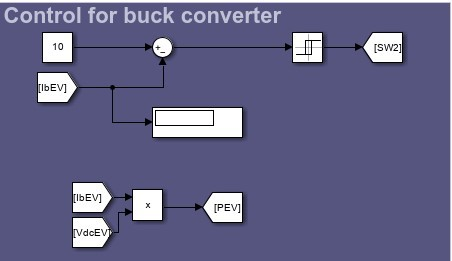
\includegraphics[width=0.8\textwidth]{Figures/buckcontrol.jpg}
    \caption{Converter for buck converter}
    \label{fig:buck_converter}
\end{figure}

\subsection{Results}

\subsubsection{Case 1}

The simulation validates the system's ability to manage power distribution dynamically. Under the defined operating scenario, the PV source successfully supplies power to both the EV load and the energy storage system (ESS). The obtained simulation results are summarized in Table~\ref{tab:case1}.

\begin{table}[H]
\centering
\caption{Simulation Results for Case 1}
\label{tab:case1}
\begin{tabular}{|l|c|}
\hline
\textbf{Parameter} & \textbf{Value} \\
\hline
DC Link Voltage & 600 V \\
EV Reference Current & 10 A \\
EV Battery Voltage & 400 V \\
Storage Battery Voltage & 400 V \\
PV Voltage at MPP & 245.4 V \\
PV Current at MPP & 34.7 A \\
PV Maximum Power & 8520 W \\
EV Battery Power & 4000 W \\
Storage Battery Power & 4520 W \\
Two-Quadrant Chopper Mode & Buck (Charging) \\
\hline
\end{tabular}
\end{table}

\paragraph{Performance Evaluation}

\begin{itemize}

\item \textbf{Load Regulation:}
The hysteresis current controller successfully regulates the EV charging current at 10 A, providing a constant charging power of approximately 4000 W despite variations in the DC bus voltage.

\item \textbf{ESS Management:}
The bidirectional converter operates in Buck mode to charge the energy storage system using the surplus PV power (4520 W). The simulation confirms efficient power transfer and accurate charging current regulation.

\item \textbf{System Stability:}
The obtained waveforms demonstrate fast transient response and stable operation of the DC bus voltage while simultaneously supplying the EV load and charging the ESS, validating the effectiveness of the overall control strategy.

\end{itemize}

\paragraph{Scopes and Displays}


%%%%%%%%%%%%%%%%%%%%%%%%%%%%%%%%%%%%%%%%%%%%%%%%%%%%%%%
\begin{figure}[H]
\centering
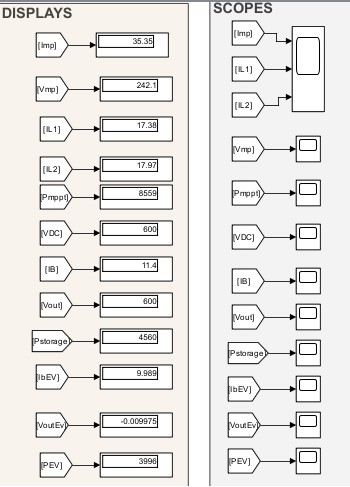
\includegraphics[width=0.8\textwidth]{Figures/yarab.jpg}
\caption{Scopes and Displays}
\label{fig:interleaved_current}
\end{figure}

\begin{figure}[H]
\centering
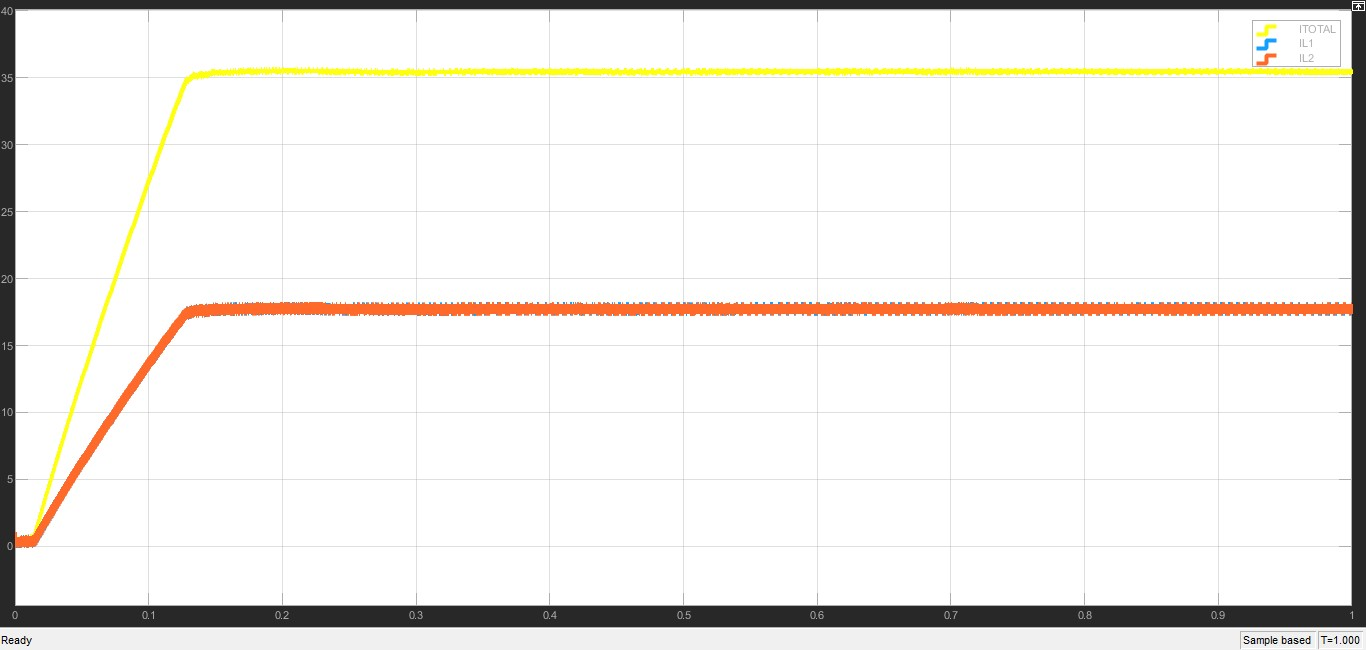
\includegraphics[width=0.8\textwidth]{Figures/Inew.jpg}
\caption{Total Input Current versus Inductor Currents ($I_{L1}$ and $I_{L2}$)}
\label{fig:interleaved_current}
\end{figure}

\begin{figure}[H]
\centering
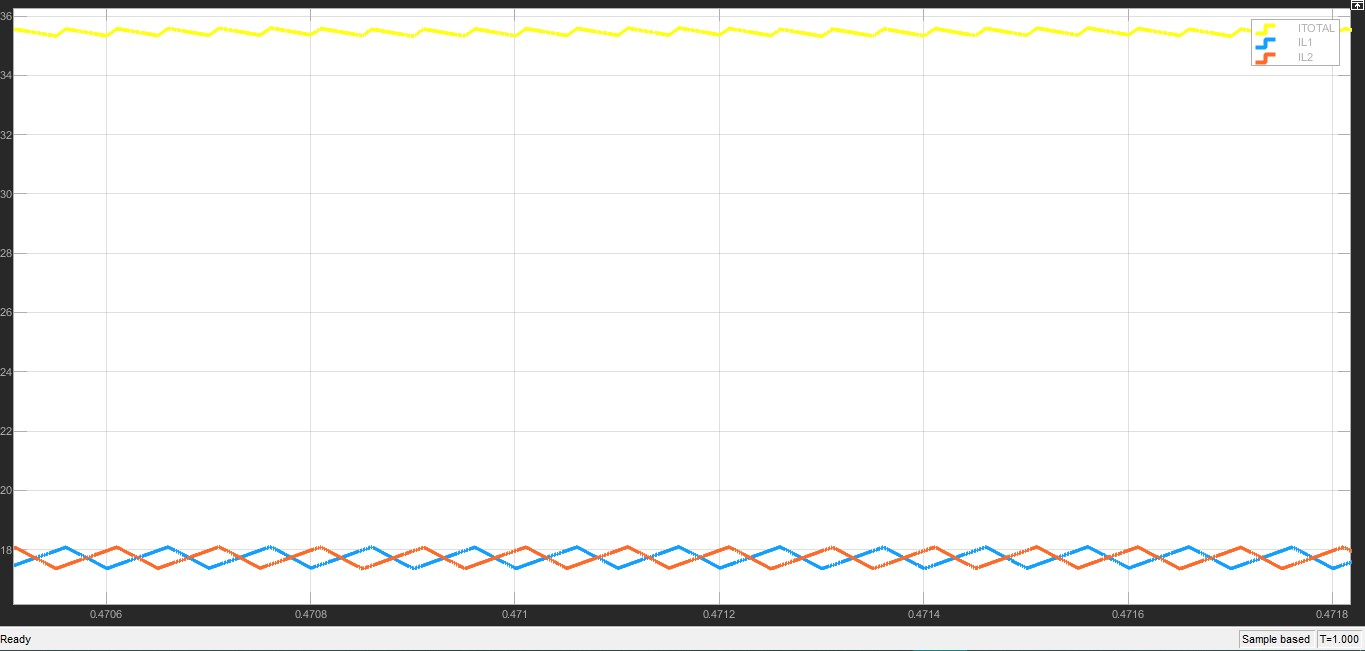
\includegraphics[width=0.8\textwidth]{Figures/I2.jpg}
\caption{ Zoom in for Total Input Current versus Inductor Currents ($I_{L1}$ and $I_{L2}$)}
\label{fig:interleaved_current}
\end{figure}
The waveform demonstrates the effectiveness of the 180$^\circ$ interleaving technique. The ripple components of the individual inductor currents cancel each other, resulting in a smoother total input current compared with a conventional single-phase boost converter.

%%%%%%%%%%%%%%%%%%%%%%%%%%%%%%%%%%%%%%%%%%%%%%%%%%%%%%%

\begin{figure}[H]
\centering
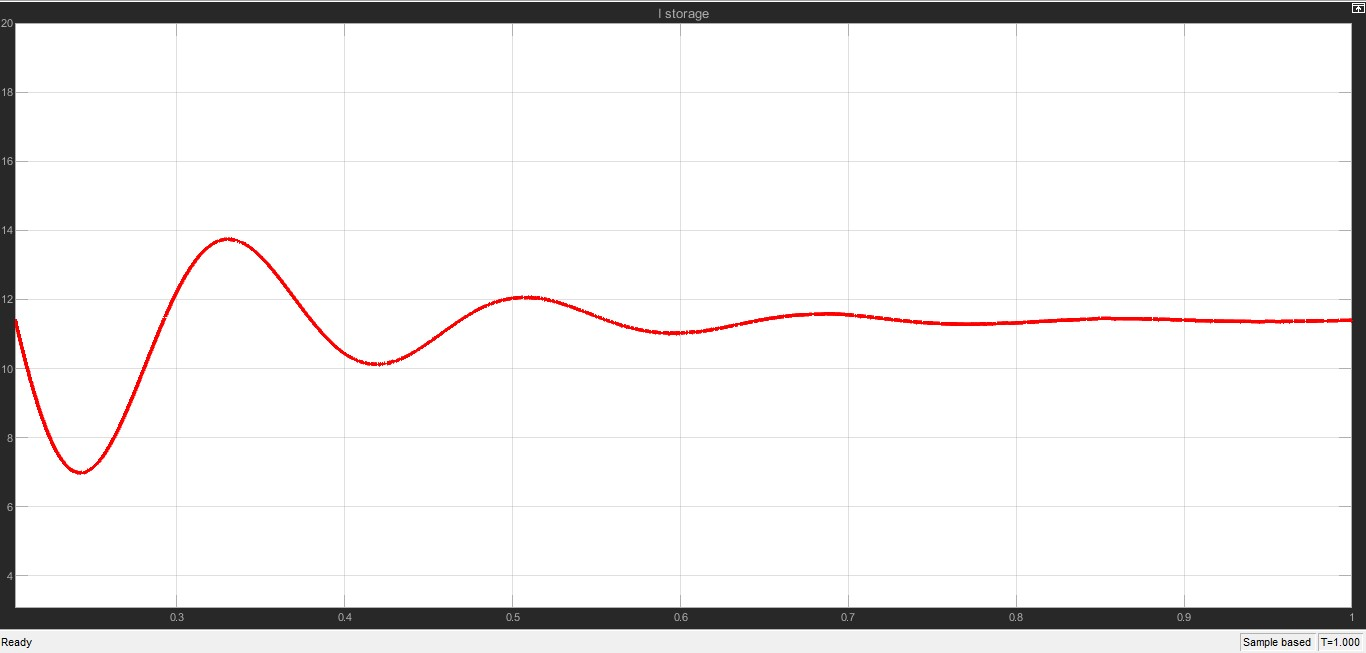
\includegraphics[width=\textwidth]{Figures/IBattery storage.jpg}
\caption{Energy Storage System (ESS) Charging Current}
\label{fig:ess_current}
\end{figure}

The waveform illustrates the transient charging response followed by a stable steady-state current, confirming the effectiveness of the PI current controller.

%%%%%%%%%%%%%%%%%%%%%%%%%%%%%%%%%%%%%%%%%%%%%%%%%%%%%%%

\begin{figure}[H]
\centering
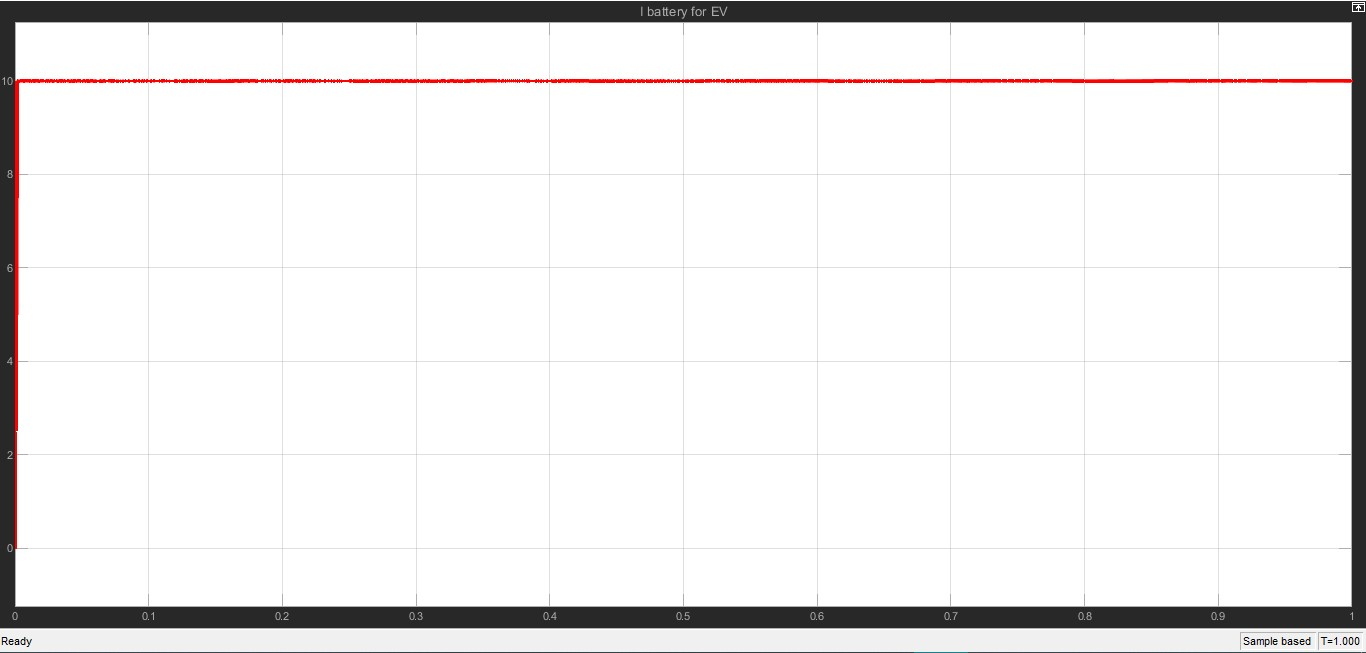
\includegraphics[width=0.8\textwidth]{Figures/iev.jpg}
\caption{EV Battery Charging Current}
\label{fig:ev_current}
\end{figure}

The hysteresis current controller maintains the EV charging current at the desired reference value of 10 A with excellent regulation accuracy.

%%%%%%%%%%%%%%%%%%%%%%%%%%%%%%%%%%%%%%%%%%%%%%%%%%%%%%%

\begin{figure}[H]
\centering
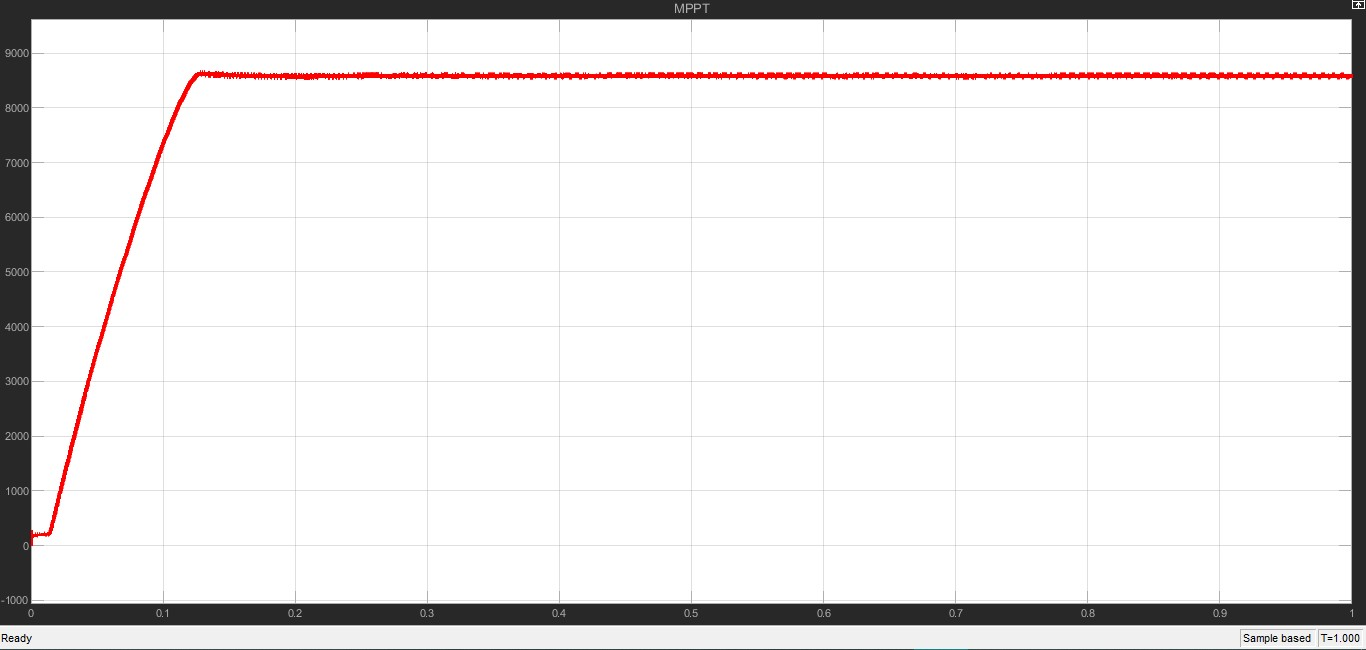
\includegraphics[width=0.8\textwidth]{Figures/pmppt.jpg}
\caption{PV Array Power Tracked by the MPPT Algorithm}
\label{fig:mppt_power}
\end{figure}

The MPPT algorithm rapidly converges to the maximum available power of approximately 8.52 kW and maintains stable operation around the maximum power point.

%%%%%%%%%%%%%%%%%%%%%%%%%%%%%%%%%%%%%%%%%%%%%%%%%%%%%%%

\begin{figure}[H]
\centering
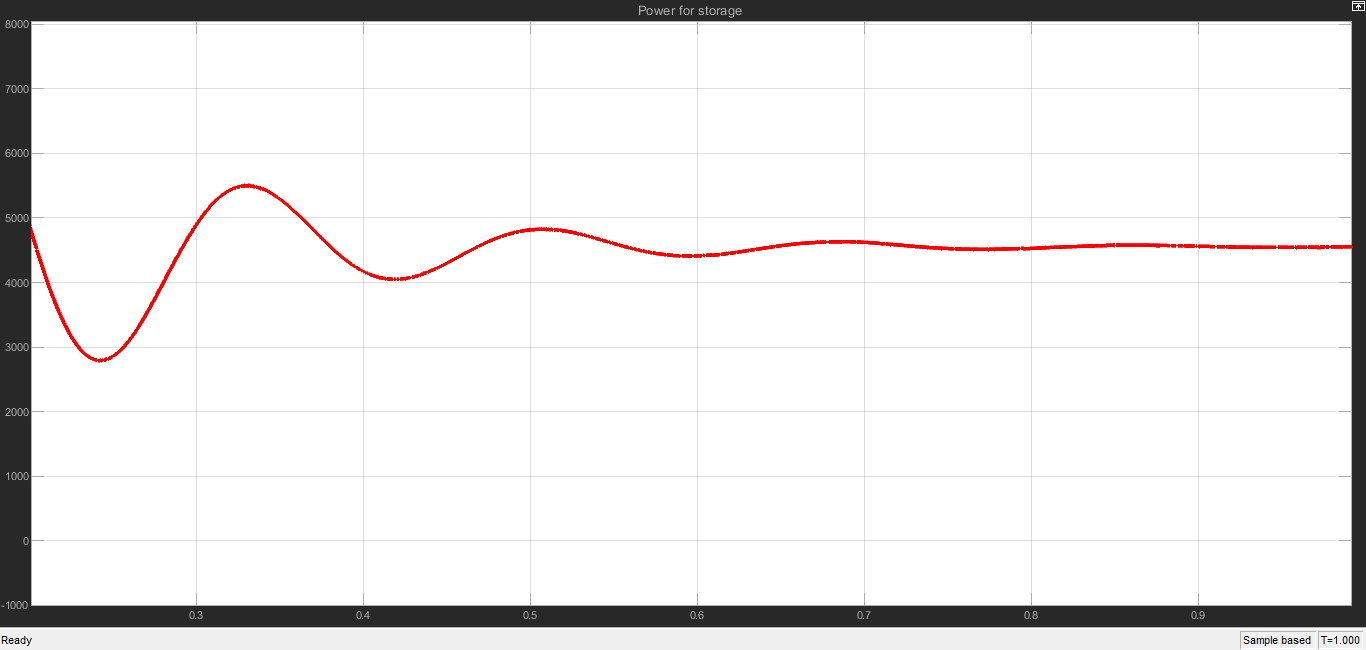
\includegraphics[width=0.8\textwidth]{Figures/pout for storage.jpg}
\caption{Storage Battery Power}
\label{fig:storage_power}
\end{figure}

The waveform confirms that approximately 4.52 kW of surplus power is efficiently transferred to the ESS during the charging process.

%%%%%%%%%%%%%%%%%%%%%%%%%%%%%%%%%%%%%%%%%%%%%%%%%%%%%%%

\begin{figure}[H]
\centering
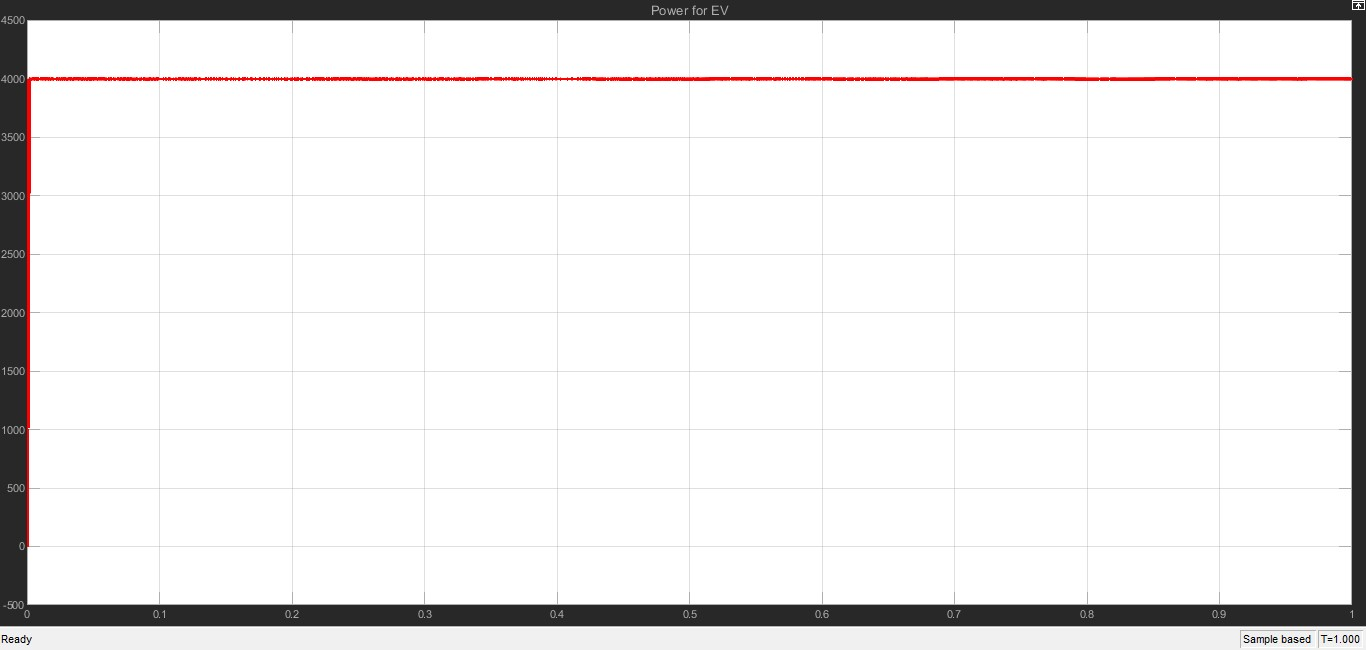
\includegraphics[width=0.8\textwidth]{Figures/Powerev.jpg}
\caption{EV Load Power}
\label{fig:ev_power}
\end{figure}

The EV charging power remains constant at approximately 4 kW, indicating stable operation throughout the charging interval.

%%%%%%%%%%%%%%%%%%%%%%%%%%%%%%%%%%%%%%%%%%%%%%%%%%%%%%%

\begin{figure}[H]
\centering
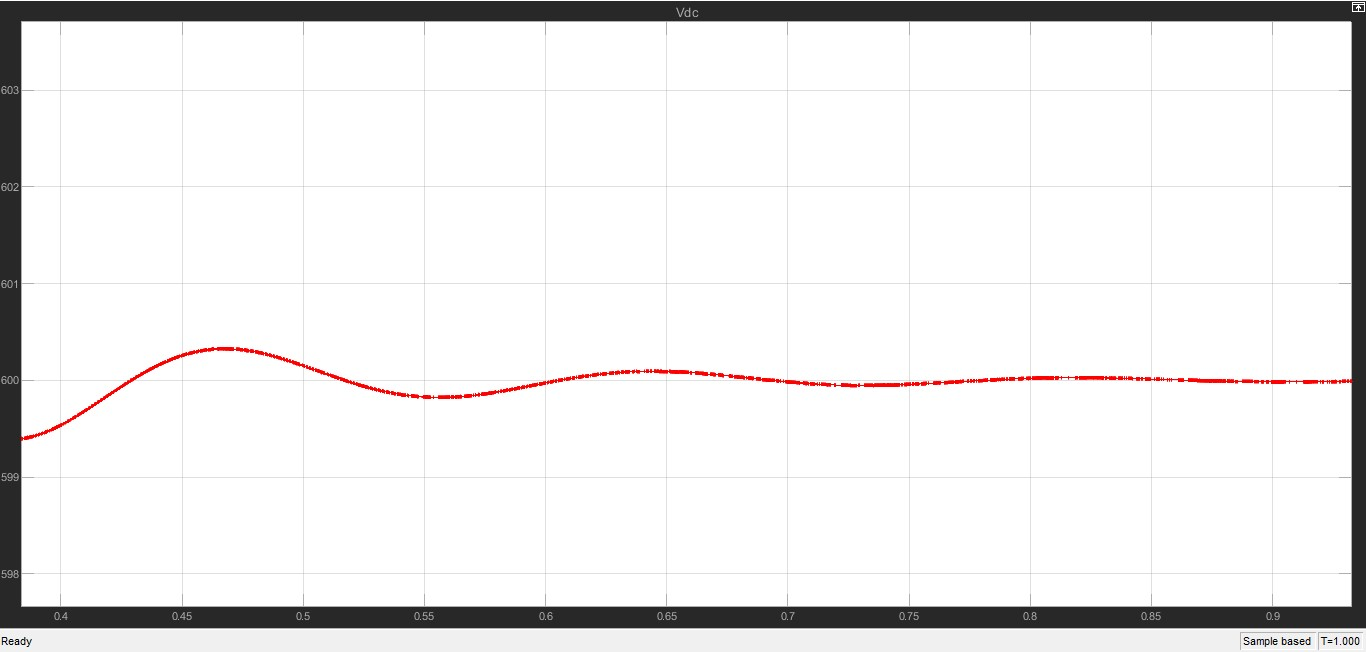
\includegraphics[width=0.8\textwidth]{Figures/vdc.jpg}
\caption{DC Bus Voltage}
\label{fig:dc_bus}
\end{figure}

The DC bus voltage is successfully regulated at 600 V with minimal ripple, demonstrating the effectiveness of the integrated control strategy.

%%%%%%%%%%%%%%%%%%%%%%%%%%%%%%%%%%%%%%%%%%%%%%%%%%%%%%%

\begin{figure}[H]
\centering
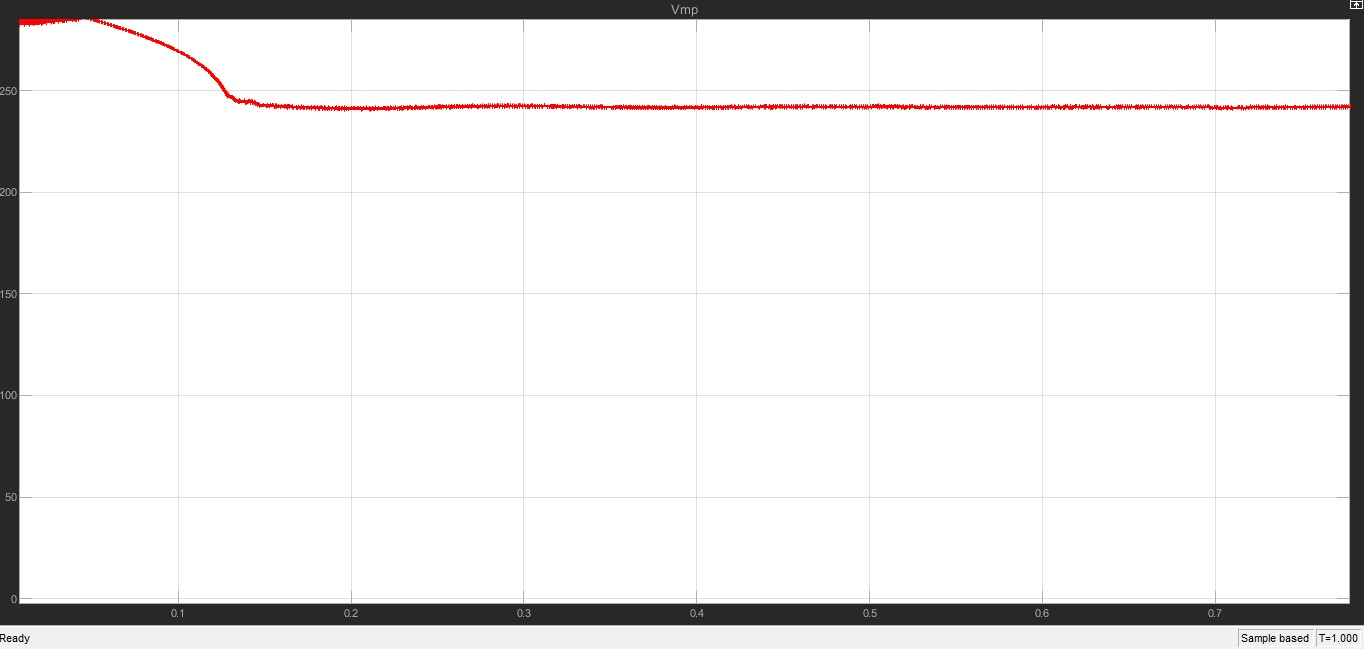
\includegraphics[width=0.8\textwidth]{Figures/vmp.jpg}
\caption{PV Array Voltage at the Maximum Power Point}
\label{fig:pv_voltage}
\end{figure}

The PV voltage remains close to the desired maximum power point voltage (245.4 V), indicating high MPPT tracking accuracy and stable converter operation.

\subsubsection{Case 2}

The simulation validates the system's ability to maintain power balance under deficit conditions, where the EV load demand exceeds the available PV generation. The system performance is summarized in Table~\ref{tab:case2}.

\begin{table}[H]
\centering
\caption{Simulation Results for Case 2}
\label{tab:case2}
\begin{tabular}{|l|c|}
\hline
\textbf{Parameter} & \textbf{Value} \\
\hline
PV Generated Power & 8520 W \\
EV Load Power & 12000 W \\
ESS Compensation Power & 3480 W (Discharging) \\
Two-Quadrant Chopper Mode & Boost (Discharging) \\
\hline
\end{tabular}
\end{table}

\paragraph{Performance Evaluation}

\begin{itemize}

\item \textbf{Power Balancing Logic:}

The simulation demonstrates that the system successfully maintains instantaneous power balance by supplying the required deficit power from the Energy Storage System (ESS). The required compensation power is

\begin{equation}
P_{ESS}=12000-8520=3480~\mathrm{W}
\end{equation}

which enables the EV load demand to be fully satisfied.

\item \textbf{Bidirectional Converter Operation:}

During this operating condition, the Two-Quadrant Chopper automatically switches to the \textbf{Boost} operating mode. The battery discharge current confirms that energy is transferred from the ESS to the DC bus while maintaining the DC bus voltage at 600 V.

\item \textbf{System Stability:}

Although the EV load requires 12 kW, the integrated control strategy successfully regulates the DC bus voltage at 600 V, demonstrating the robustness of the proposed system during power deficit conditions.

\end{itemize}

\paragraph{Scopes and Displays}

%%%%%%%%%%%%%%%%%%%%%%%%%%%%%%%%%%%%%%%%%%%%%%%%%%%%%%%%%%

\begin{figure}[H]
\centering
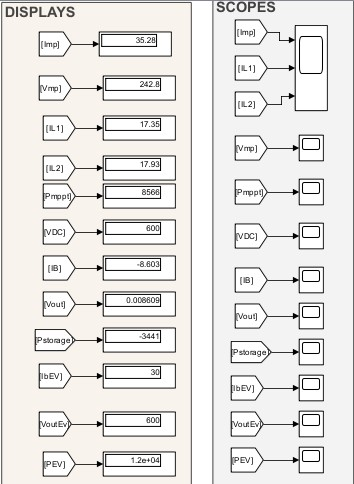
\includegraphics[width=0.9\textwidth]{Figures/SharedScreenshot.jpg}
\caption{Scopes and Displays}
\label{fig:case2_scope}
\end{figure}

%%%%%%%%%%%%%%%%%%%%%%%%%%%%%%%%%%%%%%%%%%%%%%%%%%%%%%%%%%

\begin{figure}[H]
\centering
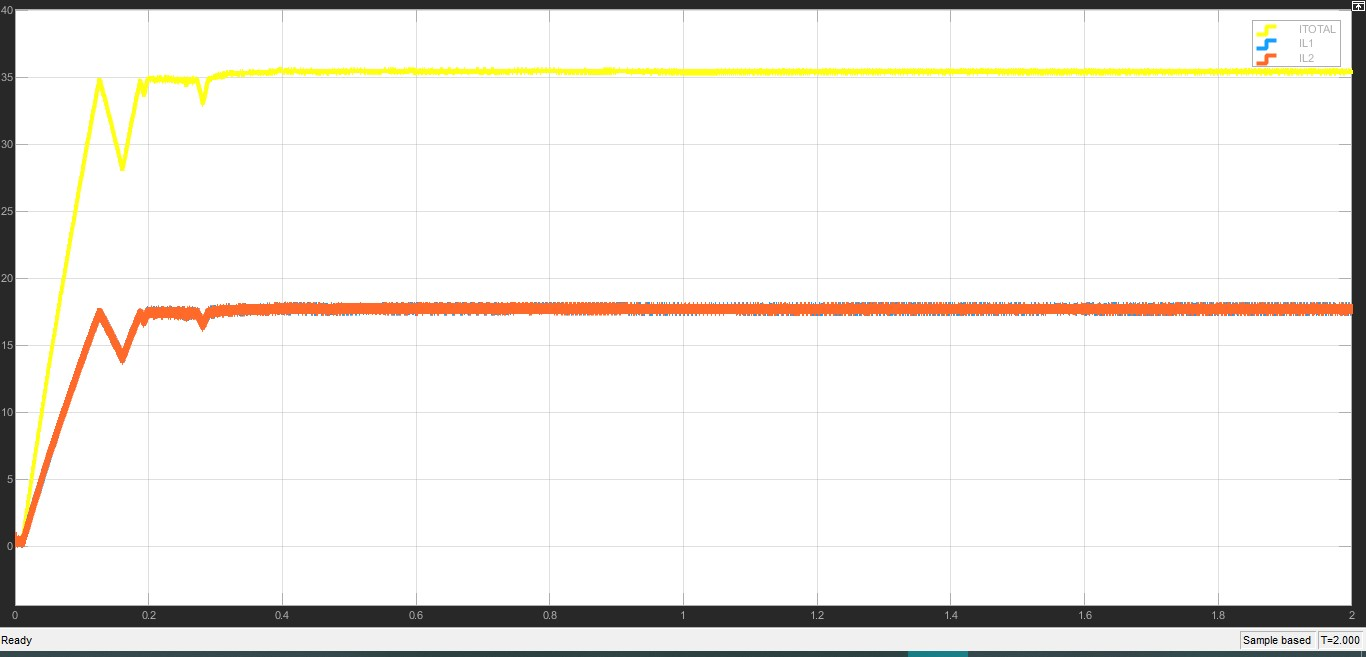
\includegraphics[width=0.85\textwidth]{Figures/case2/inew.jpg}
\caption{Interleaved Inductor Currents ($I_{L1}$ and $I_{L2}$) and Total Input Current During Boost Mode}
\label{fig:interleaved_case2}
\end{figure}

\begin{figure}[H]
\centering
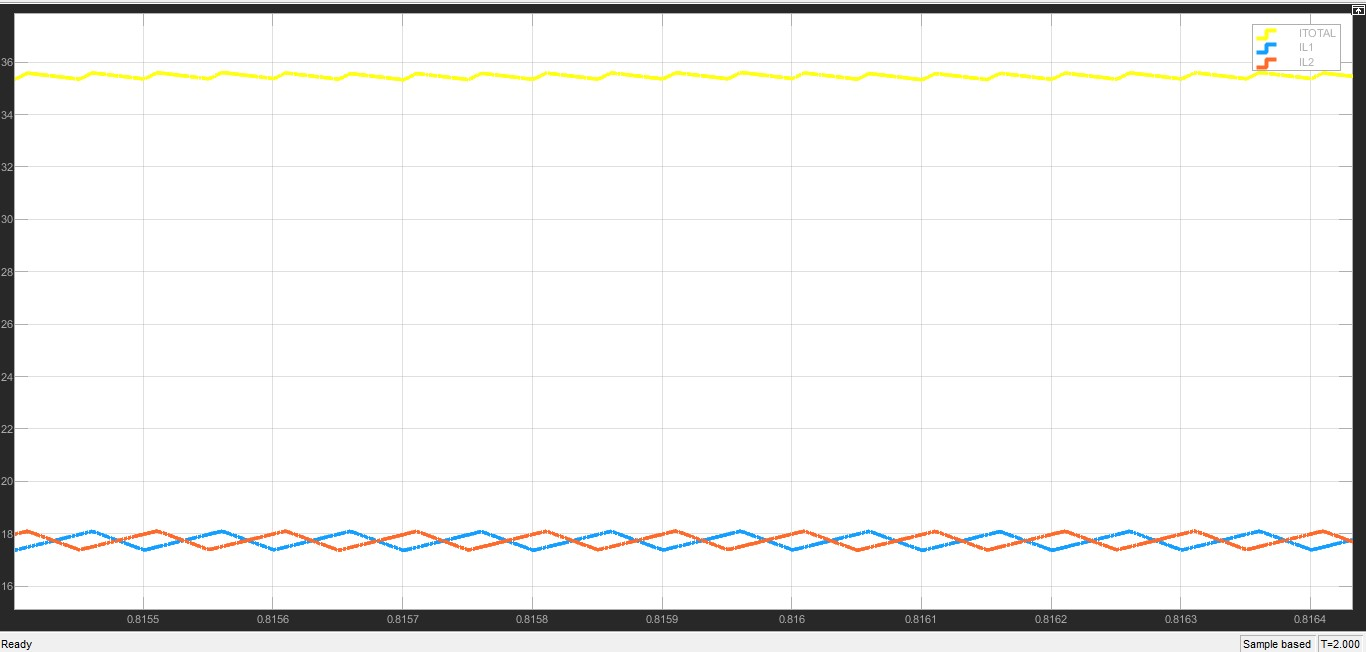
\includegraphics[width=0.85\textwidth]{Figures/case2/i2.jpg}
\caption{Zoomed View of the Interleaved Currents}
\label{fig:interleaved_zoom}
\end{figure}

The interleaved currents effectively regulate the power transfer from the ESS to the DC bus. The waveforms verify that the interleaving strategy remains stable while operating in Boost mode.

%%%%%%%%%%%%%%%%%%%%%%%%%%%%%%%%%%%%%%%%%%%%%%%%%%%%%%%%%%

\begin{figure}[H]
\centering
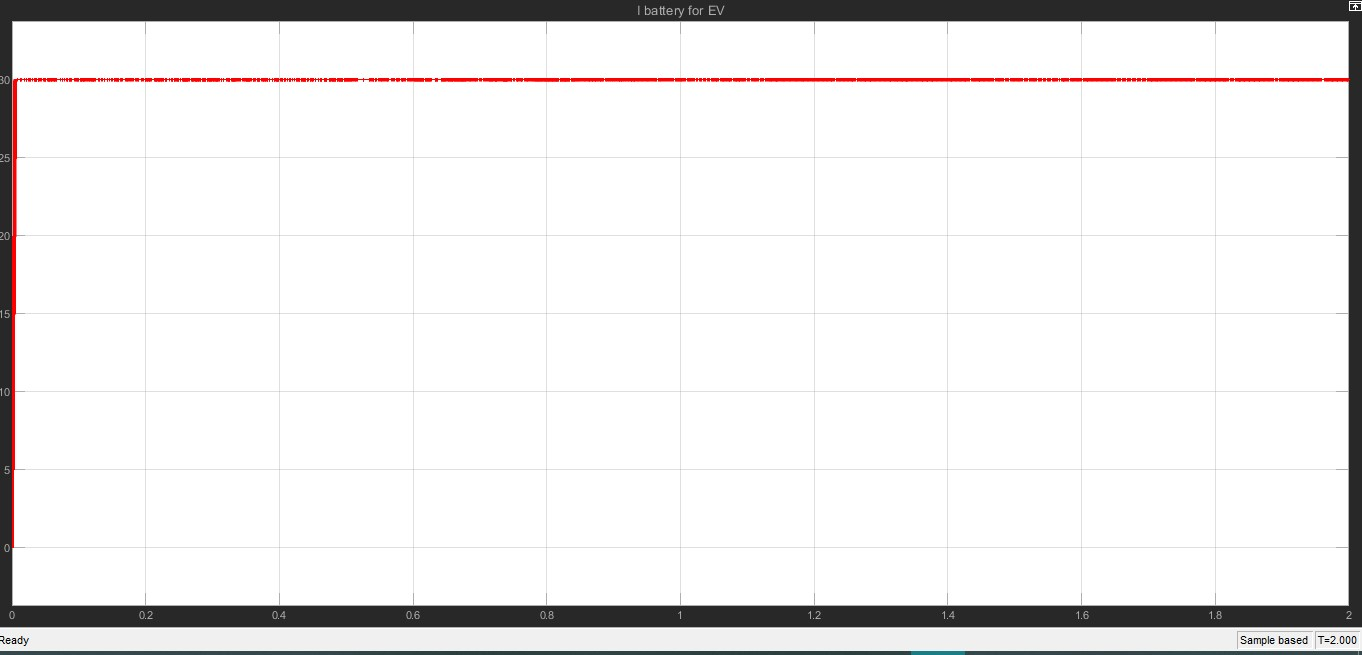
\includegraphics[width=0.85\textwidth]{Figures/case2/ibev.jpg}
\caption{EV Battery Charging Current}
\label{fig:ev_current_case2}
\end{figure}

The hysteresis current controller successfully regulates the EV charging current at the desired value of 30 A, ensuring stable power delivery even when the PV generation is insufficient.

%%%%%%%%%%%%%%%%%%%%%%%%%%%%%%%%%%%%%%%%%%%%%%%%%%%%%%%%%%

\begin{figure}[H]
\centering
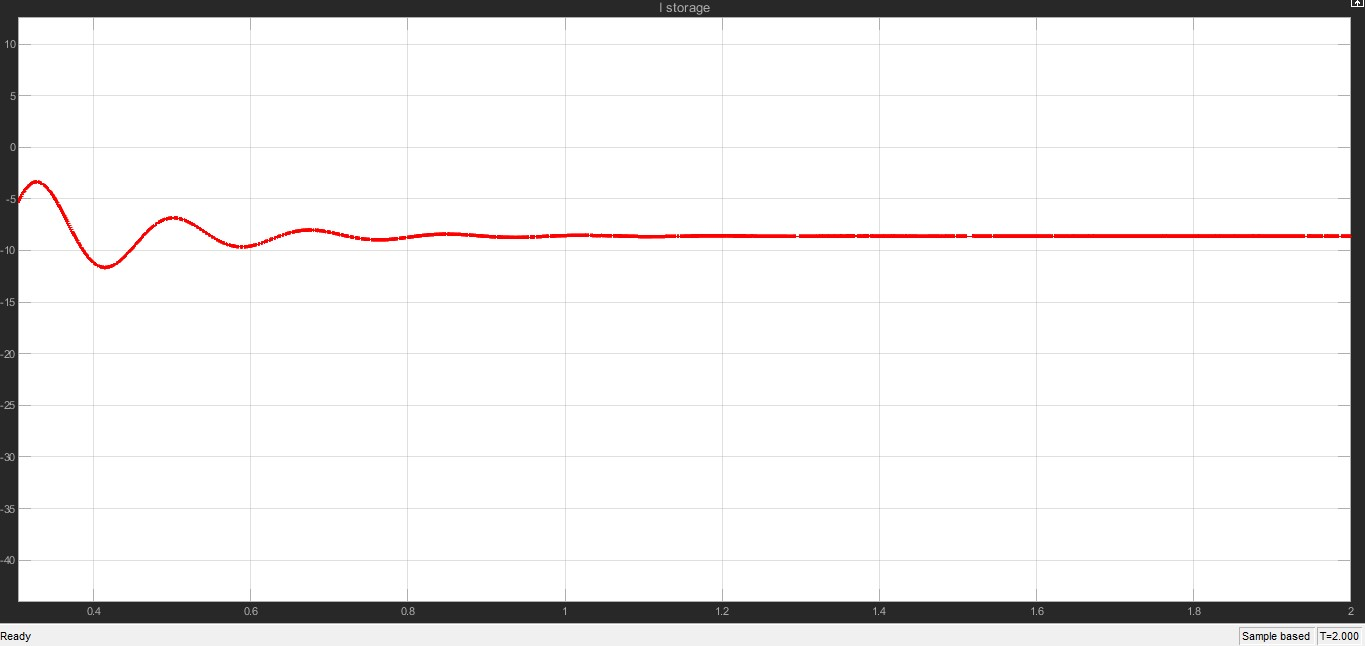
\includegraphics[width=0.85\textwidth]{Figures/case2/istorage.jpg}
\caption{ESS Discharge Current}
\label{fig:ess_discharge}
\end{figure}

The negative battery current indicates that the Energy Storage System is discharging and supplying approximately 3480 W to compensate for the deficit between the PV generation and the EV load demand.

%%%%%%%%%%%%%%%%%%%%%%%%%%%%%%%%%%%%%%%%%%%%%%%%%%%%%%%%%%

\begin{figure}[H]
\centering
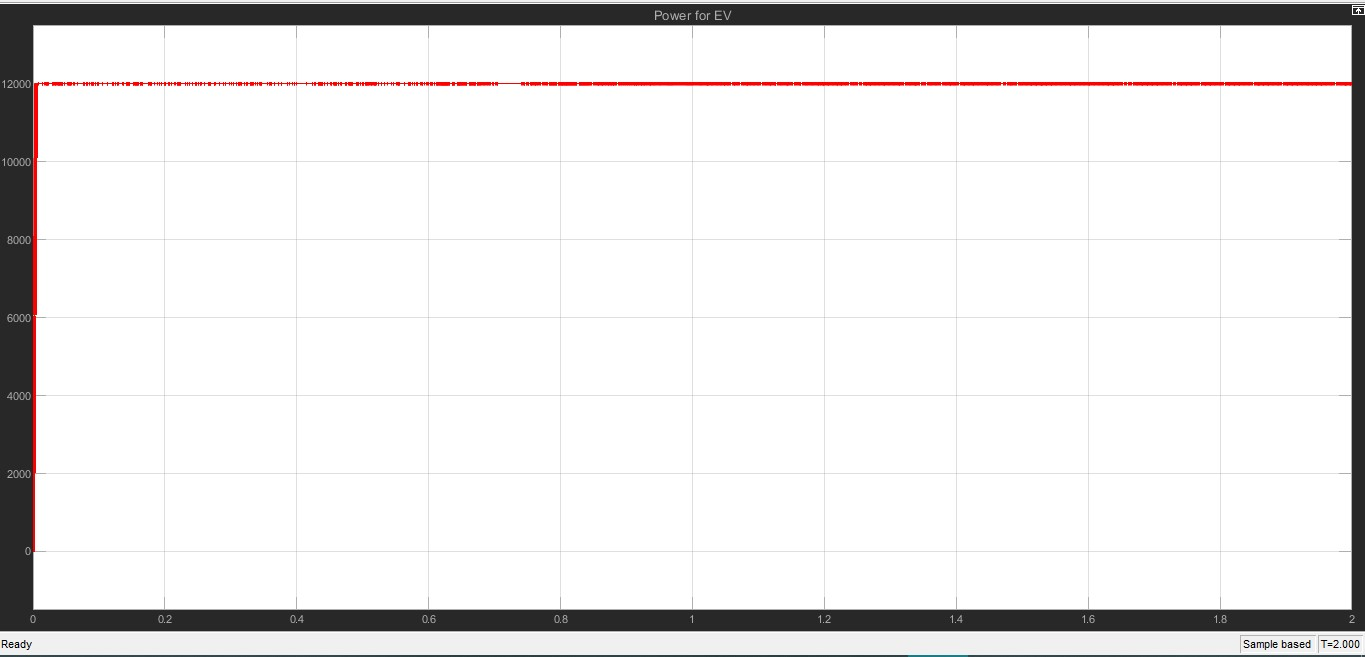
\includegraphics[width=0.85\textwidth]{Figures/case2/pev.jpg}
\caption{EV Load Power}
\label{fig:ev_power_case2}
\end{figure}

The EV load continuously receives the required 12 kW, demonstrating the capability of the proposed system to satisfy high load demand.

%%%%%%%%%%%%%%%%%%%%%%%%%%%%%%%%%%%%%%%%%%%%%%%%%%%%%%%%%%

\begin{figure}[H]
\centering
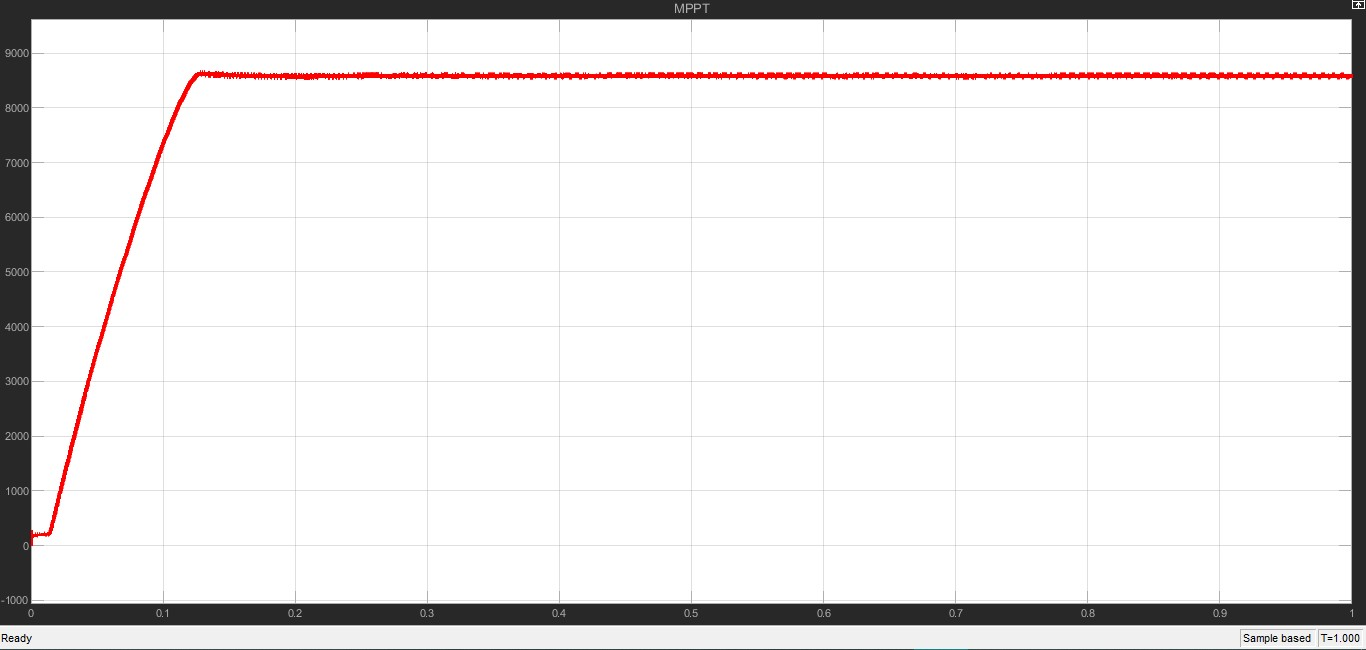
\includegraphics[width=0.85\textwidth]{Figures/pmppt.jpg}
\caption{PV Array Output Power}
\label{fig:pv_power_case2}
\end{figure}

The MPPT algorithm continuously tracks the maximum available power from the PV array and maintains an output power of approximately 8.52 kW.

%%%%%%%%%%%%%%%%%%%%%%%%%%%%%%%%%%%%%%%%%%%%%%%%%%%%%%%%%%

\begin{figure}[H]
\centering
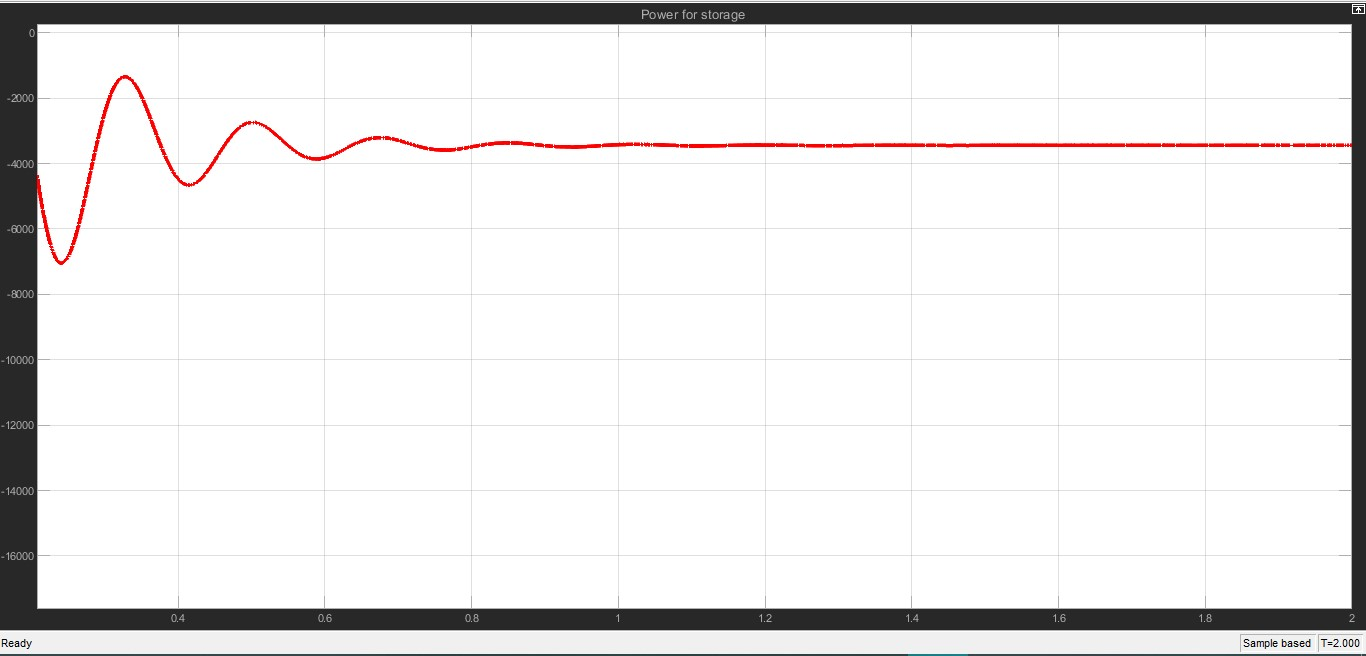
\includegraphics[width=0.85\textwidth]{Figures/case2/pstorage.jpg}
\caption{ESS Power Flow}
\label{fig:ess_power_case2}
\end{figure}

The waveform confirms that approximately 3480 W is delivered from the ESS to the DC bus, maintaining the required system power balance.

%%%%%%%%%%%%%%%%%%%%%%%%%%%%%%%%%%%%%%%%%%%%%%%%%%%%%%%%%%

\begin{figure}[H]
\centering
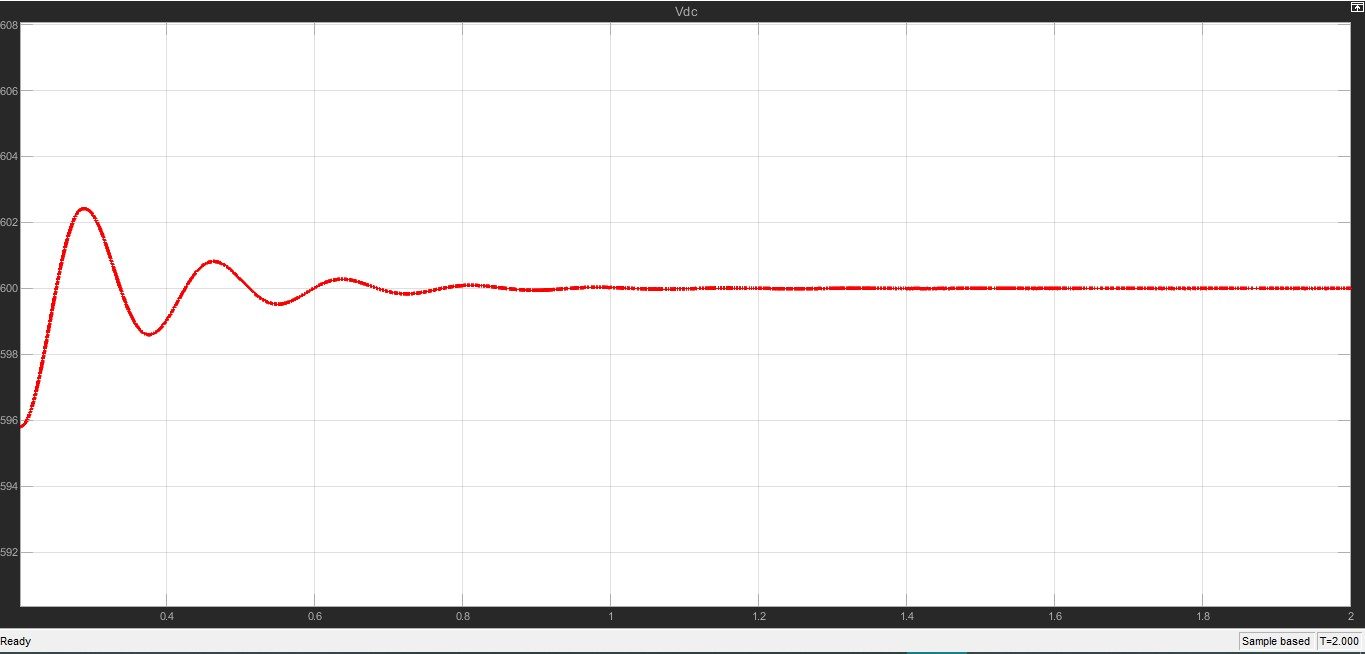
\includegraphics[width=0.85\textwidth]{Figures/case2/vdc.jpg}
\caption{DC Bus Voltage}
\label{fig:dcbus_case2}
\end{figure}

The DC bus voltage remains tightly regulated around 600 V throughout the Boost mode operation, confirming the effectiveness of the proposed control strategy.

%%%%%%%%%%%%%%%%%%%%%%%%%%%%%%%%%%%%%%%%%%%%%%%%%%%%%%%%%%

\begin{figure}[H]
\centering
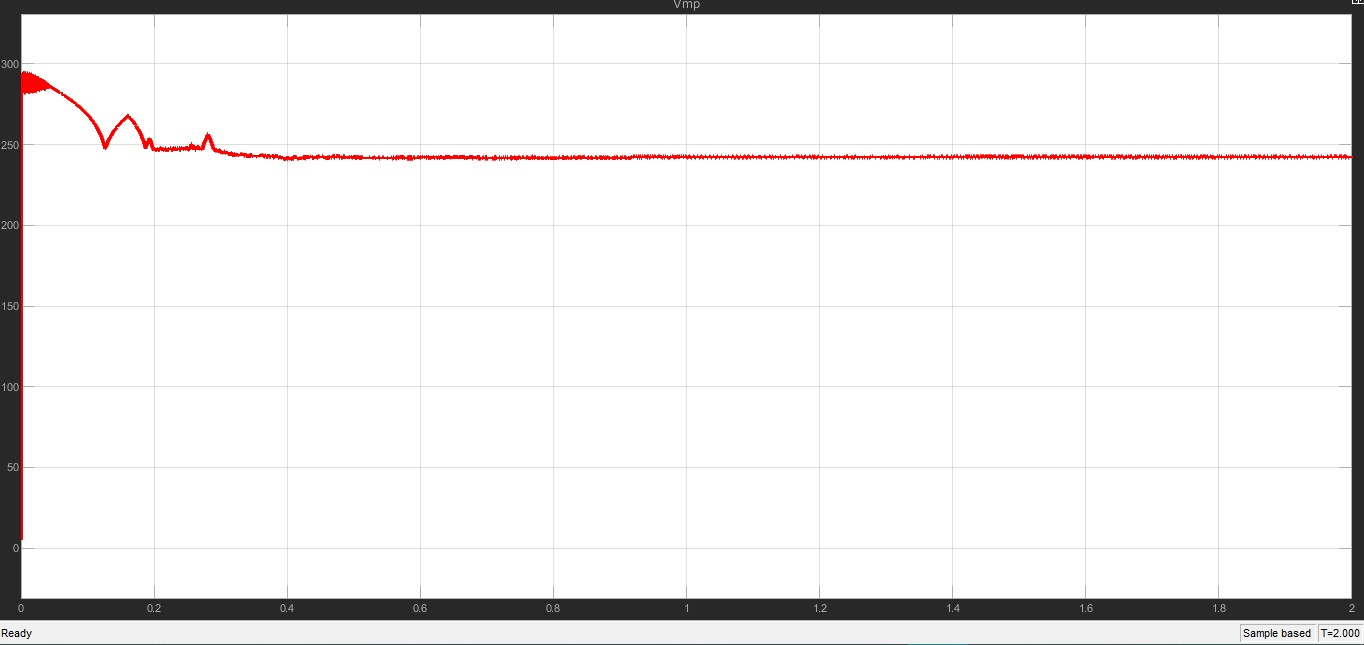
\includegraphics[width=0.85\textwidth]{Figures/case2/vmpt.jpg}
\caption{PV Voltage at the Maximum Power Point}
\label{fig:pv_voltage_case2}
\end{figure}

The PV voltage remains close to the maximum power point voltage, demonstrating accurate MPPT tracking and efficient utilization of the available solar energy.

\end{itemize}
\section{Central Interleaved Boost (Actual Ratings)}

In modern engineering, jumping straight from a conceptual design to physical hardware is a risky and costly approach. Simulation serves as the crucial bridge between theory and reality. By creating a high-fidelity digital twin of a system, designers can validate control logic, analyze transient behaviors, and stress-test components under extreme conditions without the risk of catastrophic hardware failure.

so before doing anything hardware, we must first do simulation of the circuit to fully understand the it and test different faults or errors that we might face.

\subsection{Simulation of Central Boost without MPPT}
R with mosfet asts as a storage system used to mantain voltage of the dc link at 10\,V with hysteresis control
here is the test to see which duty will achieve max power:
\begin{figure}[H]
    \centering
    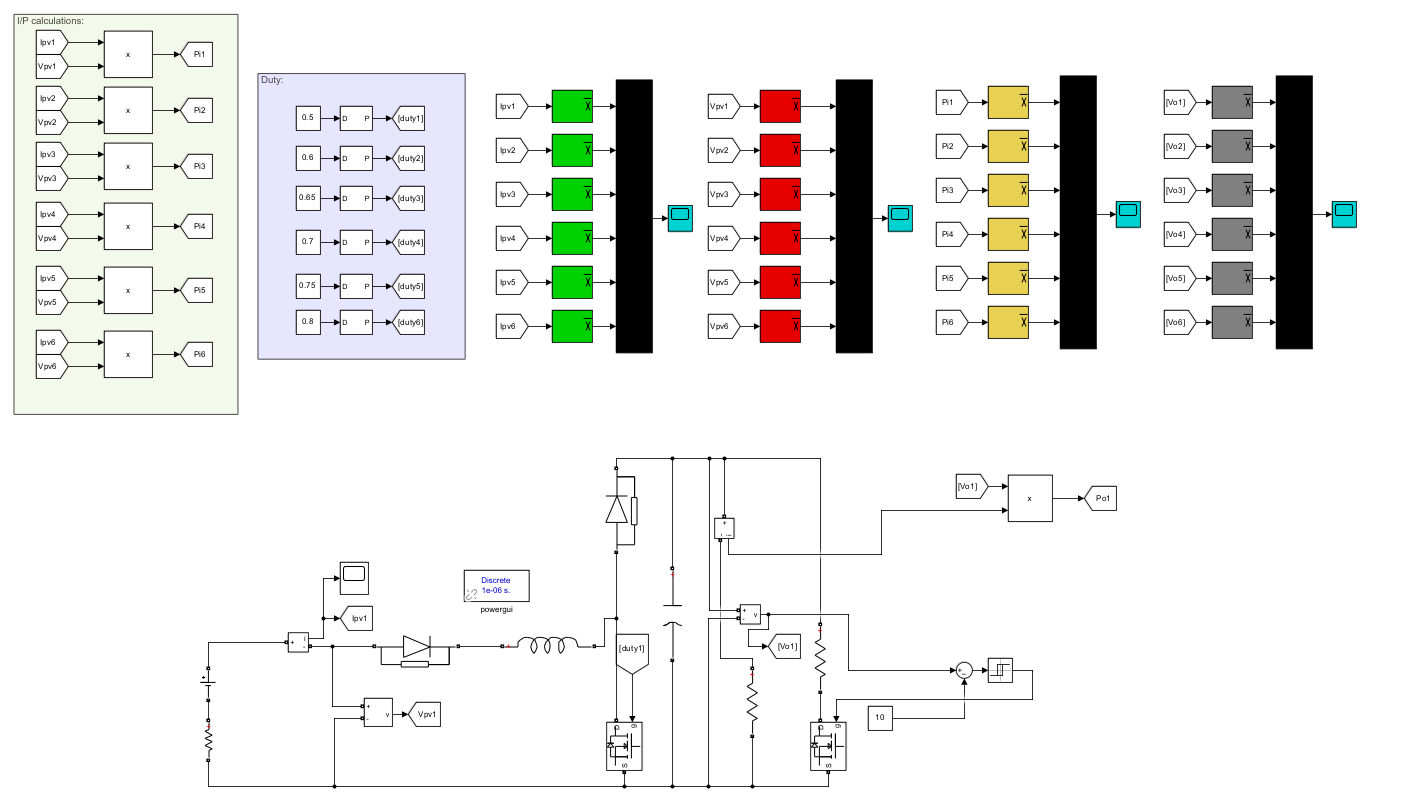
\includegraphics[width=0.85\textwidth]{Figures/5.5.1.png}
    \caption{Central Boost.}
    \label{fig:central boost actual ratings}
\end{figure}

To evaluate the dynamic stability of the system under localized storage integration, the complex photovoltaic (PV) array non-linear characteristic curve is simplified around its operating point utilizing a linear Thevenin equivalent circuit interface. The voltage source and its series internal impedance parameters are defined as:
\begin{itemize}
    \item Thevenin Voltage ($V_{\text{th}}$): $12\text{ V}$
    \item Internal Thevenin Resistance ($R_{\text{th}}$): $6.8\ \Omega$
\end{itemize}

\subsubsection{Hysteresis-Controlled Storage Branch}
A secondary power branch containing a switching MOSFET in series with a storage resistor ($R_{\text{storage}} = 47\ \Omega$) serves as a dynamic energy buffer. This subsystem actively regulates and clamps the output high-voltage DC-link bus at a rigid target command of $V_{\text{DC\_ref}} = 10\text{ V}$. 
\newpage
The regulation is driven by hysteresis control loop tracking the instantaneous DC-link voltage error. The mathematical switching states governing the gate-drive command ($S$) of the storage MOSFET are defined according to the following boundary conditions:

\begin{equation}
    S = 
    \begin{cases} 
      1 & \text{for } V_{\text{DC}} > V_{\text{DC\_ref}} + \Delta H \\
      0 & \text{for } V_{\text{DC}} < V_{\text{DC\_ref}} - \Delta H 
    \end{cases}
\end{equation}

Where $\Delta H$ represents the predefined narrow hysteresis band offset. When the DC-link voltage surpasses the upper boundary threshold, the MOSFET switches to its conduction state ($S=1$), shunting the excess power into $R_{\text{storage}}$ to discharge the bus. Conversely, when the bus voltage drops below the lower band margin, the switch opens ($S=0$) to isolate the storage asset and restore the system voltage envelope across the static load network ($R_{\text{load}} = 100\ \Omega$).

\subsubsection{System Passive Components}
The passive filtering parameters chosen to restrict high-frequency switching ripples within the network are summarized in Table \ref{tab:thevenin_parameters}.

\begin{table}[htbp]
    \centering
    \caption{Thevenin equivalent system and filter parameter metrics.}
    \label{tab:thevenin_parameters}
    \small
    \begin{tabular}{|c|c|c|}
        \hline
        \textbf{Parameter Name} & \textbf{Designation Symbol} & \textbf{Assigned Value} \\ \hline
        Inductance       & $L$                        & $2\text{ mH}$           \\ \hline
        Capacitance      & $C$                        & $2.2\text{ mF}$         \\ \hline
        Storage Resistance      & $R_{\text{storage}}$       & $47\ \Omega$            \\ \hline
        Equivalent Load         & $R_{\text{load}}$          & $100\ \Omega$           \\ \hline
    \end{tabular}
\end{table}

\subsubsection{Results}
\begin{figure}[H]
    \centering
    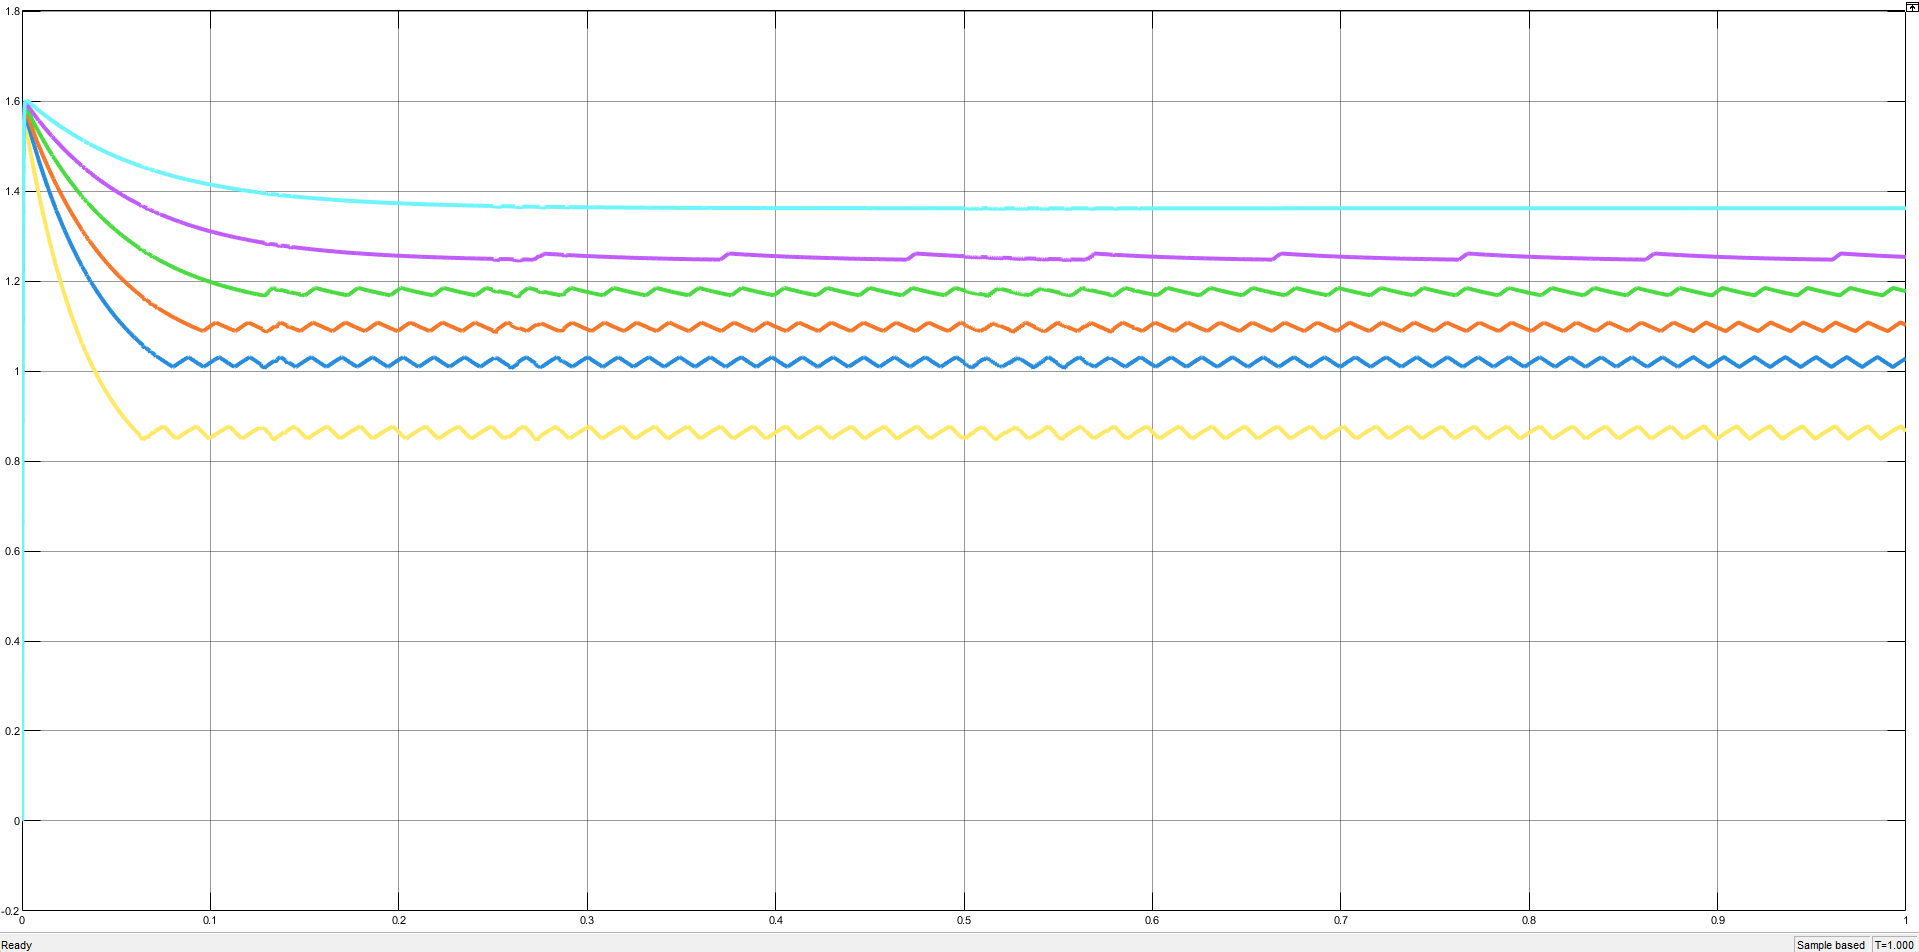
\includegraphics[width=0.9\textwidth]{Figures/5.5.2.png}
    \caption{Input Currents.}
    \label{fig: input current of central interleaved boost actual ratings}
\end{figure}
\begin{figure}[H]
    \centering
    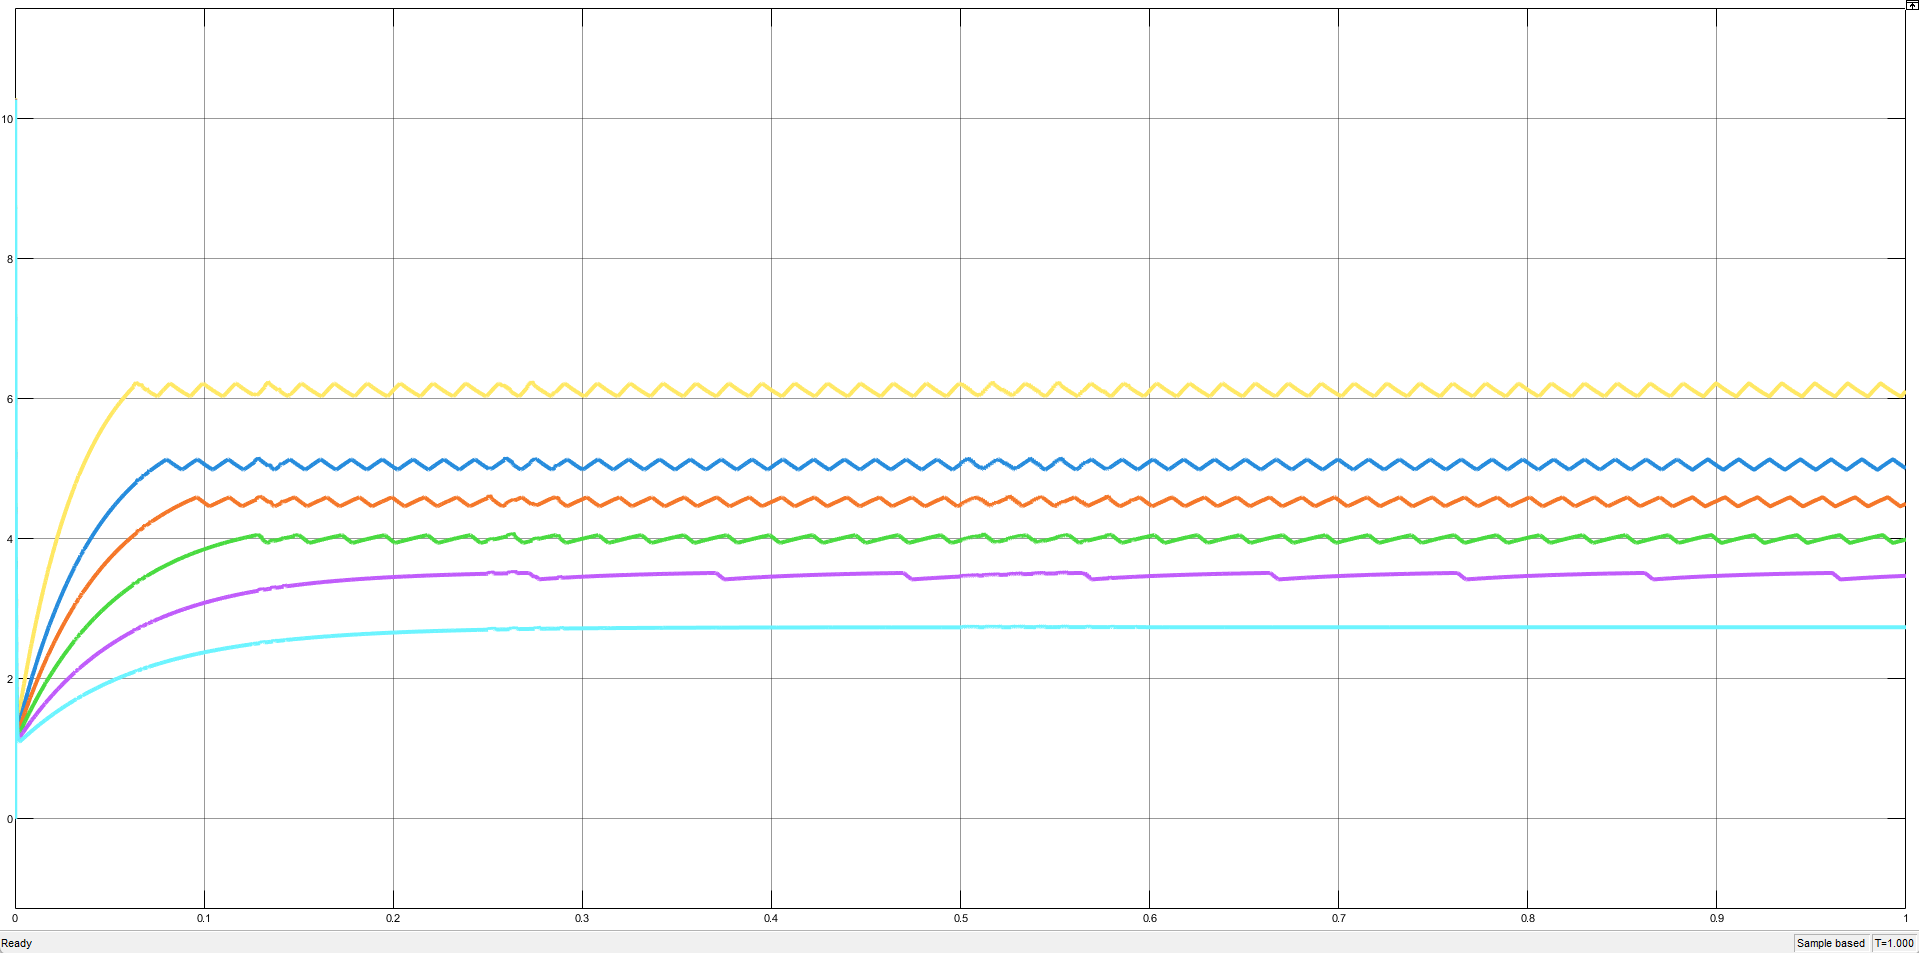
\includegraphics[width=0.9\textwidth]{Figures/5.5.3.png}
    \caption{Input Voltages.}
    \label{fig: input voltages of central interleaved boost actual ratings}
\end{figure}
\begin{figure}[H]
    \centering
    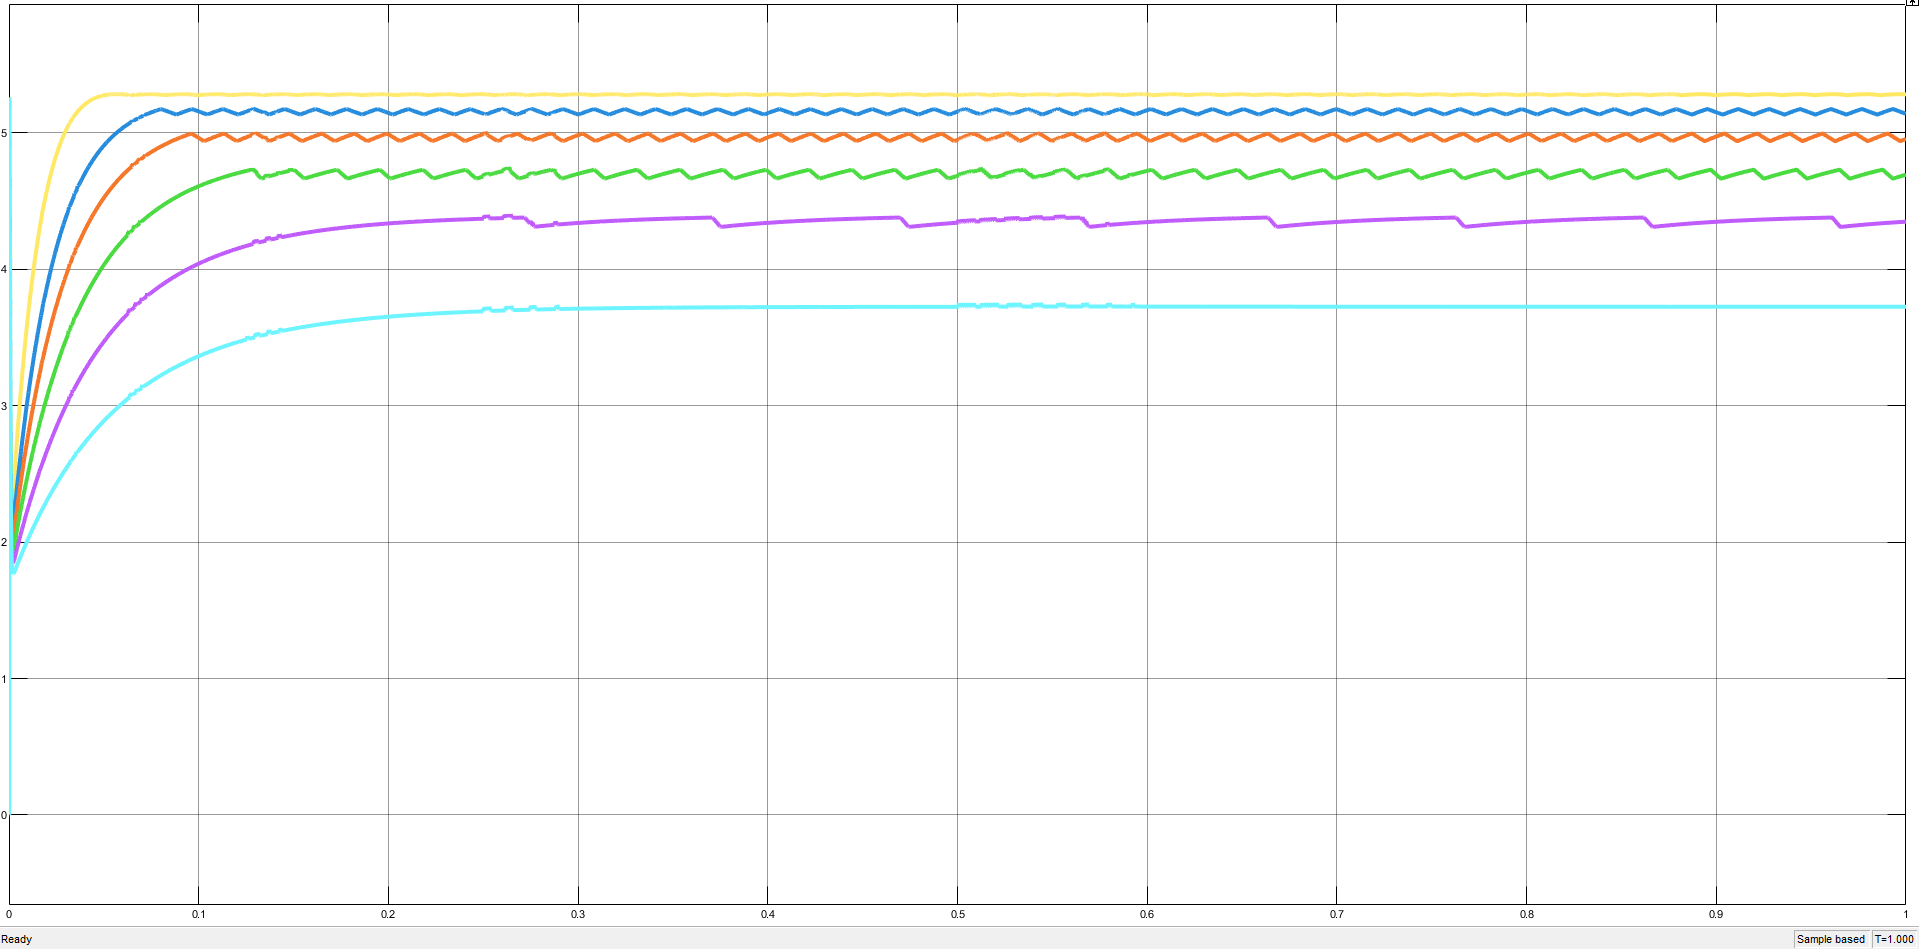
\includegraphics[width=0.9\textwidth]{Figures/5.5.4.png}
    \caption{Input Power.}
    \label{fig: input power of central interleaved boost actual ratings}
\end{figure}
\begin{figure}[H]
    \centering
    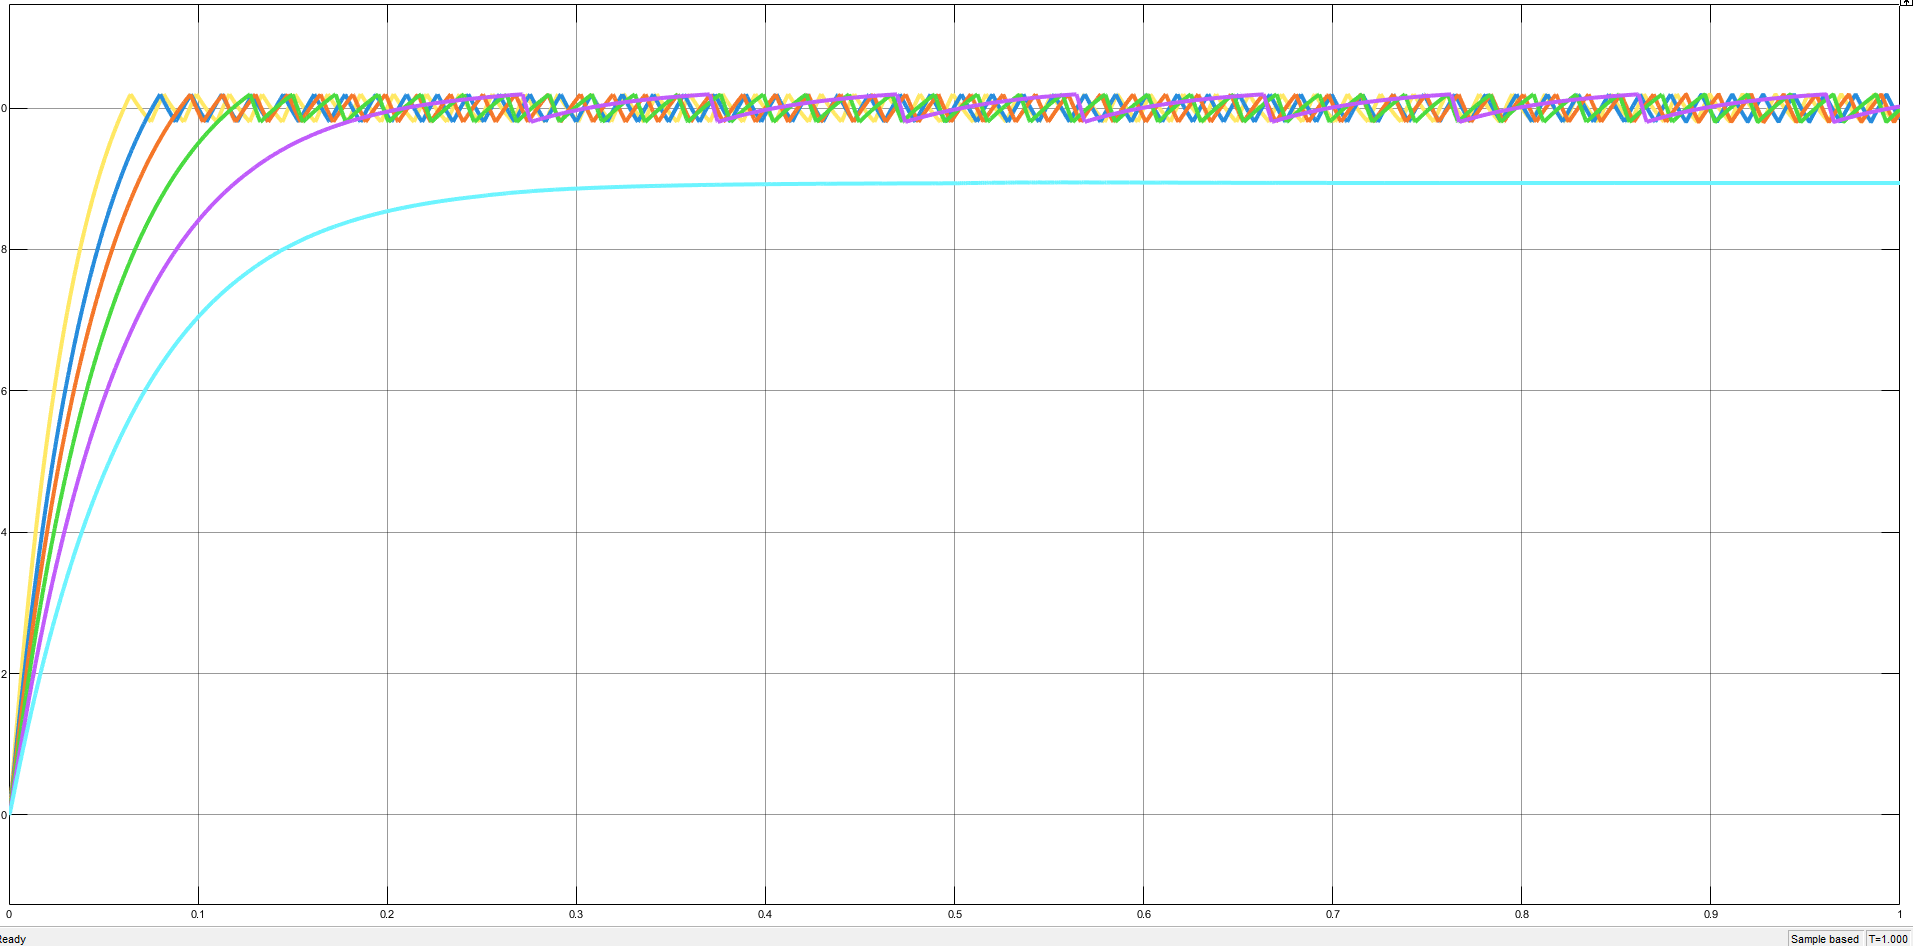
\includegraphics[width=0.9\textwidth]{Figures/5.5.5.png}
    \caption{Output Voltages.}
    \label{fig: output voltages of central interleaved boost actual ratings}
\end{figure}

As shown in the simulation results, the maximum power extraction point occurs precisely at a duty cycle of $D = 0.65$.

\subsection{Simulation of Central Interleaved Boost with MPPT}
\begin{figure}[H]
    \centering
    \includegraphics[width=0.9\textwidth]{Figures/5.5.6.png}
    \caption{Central Interleaved Boost.}
    \label{fig:central interleaved boost actual ratings}
\end{figure}

\begin{lstlisting}[language=Matlab, caption={MATLAB code implementing the FSM-based global MPPT control loop.}]
function [g1, g2] = mppt_controller_pwm(Vpv, Ipv, IL1)
    persistent V_target Pmax Vbest mode timer;
    persistent err_int_v err_int_i t;
    
    Ts = 1e-6;      
    fsw = 10e3;     
    Tsw = 1/fsw;
    
    if isempty(V_target)
        V_target = Vpv; 
        Pmax = 0;
        Vbest = Vpv;
        mode = 0;
        timer = 0;
        err_int_v = 0;
        err_int_i = 0;
        t = 0;
    end
    
    % ===== Internal Calculation of IL2 =====
    % Based on the nodal equation: Ipv = IL1 + IL2
    IL2 = Ipv - IL1; 
    
    % ===== MPPT Logic (Scanning) =====
    Ppv = Vpv * Ipv;
    V_ramp_rate = 200; 
    
    switch mode
        case 0 % Initialization
            V_target = Vpv;
            Pmax = 0;
            mode = 1;
            
        case 1 % Scanning Downward
            if Ppv > Pmax
                Pmax = Ppv;
                Vbest = Vpv;
            end
            V_target = V_target - (V_ramp_rate * Ts);
            % Stop scan at 50% of starting voltage
            if V_target <= 0.5 * Vbest 
                mode = 2;
            end
            
        case 2 % Return to Vbest
            V_target = Vbest;
            mode = 3;
            timer = 0;
            
        case 3 % Hold and Dwell
            timer = timer + Ts;
            if timer >= 5 
                mode = 0; % Restart scan
            end
    end
    
    % ===== Outer Loop: Voltage Control (Vpv -> Iref) =====
    err_v = Vpv - V_target; 
    
    Kp_v = 1.5; 
    Ki_v = 80;
    
    err_int_v = err_int_v + err_v * Ts;
    err_int_v = max(min(err_int_v, 0.5), -0.5); 
    
    Iref_total = Kp_v * err_v + Ki_v * err_int_v; 
    Iref_total = max(min(Iref_total, 20), 0); 
    
    % ===== Inner Loop: Current Control (Iref -> Duty) =====
    Iref_phase = 0.5 * Iref_total;
    
    err_i1 = Iref_phase - IL1;
    err_i2 = Iref_phase - IL2;
    
    Kp_i = 5; 
    Ki_i = 100;
    
    err_int_i = err_int_i + (err_i1 + err_i2) * Ts; 
    err_int_i = max(min(err_int_i, 10), -10);
    
    % Duty cycle calculation
    duty1 = Kp_i * err_i1 + Ki_i * err_int_i;
    duty2 = Kp_i * err_i2 + Ki_i * err_int_i;
    
    % Safety Clamps
    duty1 = max(min(duty1, 0.9), 0.1);
    duty2 = max(min(duty2, 0.9), 0.1);
    
    % ===== PWM Generation (180 deg Phase Shift) =====
    t = t + Ts;
    if t >= Tsw, t = 0; end 
    
    carrier1 = t / Tsw;
    carrier2 = mod(t + Tsw/2, Tsw) / Tsw;
    
    % ===== Gate signals =====
    g1 = (duty1 > carrier1);
    g2 = (duty2 > carrier2);
end
\end{lstlisting}

% =========================================================================
% TWO-PHASE INTERLEAVED MPPT FUNCTION CODE BREAKDOWN
% =========================================================================

\subsubsection{MATLAB Interleaved MPPT PWM Function Operational Breakdown}
The updated MATLAB Function block implements an integrated control loop that handles Global Maximum Power Point Tracking (GMPPT), cascaded dual-loop control (outer voltage and inner current loop), and direct interleaved PWM generation inside a single function block. The code operates line-by-line as follows:

\begin{itemize}
    \item \textbf{Lines 2--17: Persistent Variable and Parameter Initialization} \\
    The algorithm defines memory-persistent internal registers to track the target voltage reference ($V_{\text{target}}$), maximum logged power ($P_{\text{max}}$), optimal tracking voltage ($V_{\text{best}}$), Finite State Machine ($mode$), tracking sample timer ($timer$), control loop integration error terms ($err_{\text{int\_v}}, err_{\text{int\_i}}$), and a local time counter ($t$). Upon compilation or startup, these registers are initialized, setting the baseline parameters and establishing a sample step time of $T_s = 1\ \mu\text{s}$ and a gating switching frequency of $f_{sw} = 10\text{ kHz}$ ($T_{sw} = 100\ \mu\text{s}$).
\newpage
    \item \textbf{Lines 19--21: Sensor Node Interpolation for Phase Current $I_{L2}$} \\
    To minimize physical hardware sensor count, the code computes the second phase inductor current ($I_{L2}$) using a basic circuit nodal KCL relationship at the converter input node:
    \begin{equation}
        I_{L2} = I_{\text{pv}} - I_{L1}
    \end{equation}
    This mathematical extraction avoids needing a secondary physical current sensor while accurately tracking the current passing through the second interleaved branch.

    \item \textbf{Lines 23--49: Finite State Machine Optimization Tracking} \\
    The controller continuously samples the electrical output metrics ($P_{\text{pv}} = V_{\text{pv}} \times I_{\text{pv}}$) and runs a linear scanning sweep via four distinct operational modes:
    \begin{itemize}
        \item \textbf{Mode 0 (Initialization):} Locks onto the instantaneous panel voltage and advances directly to the scan state.
        \item \textbf{Mode 1 (Scanning Downward):} Linearly decreases the command voltage reference at a ramp rate of $V_{\text{ramp\_rate}} = 200\text{ V/s}$ ($0.0002\text{ V}$ per execution step). It continuously updates $P_{\text{max}}$ and records the corresponding optimal coordinate ($V_{\text{best}} = V_{\text{pv}}$) until the sweep threshold falls to $50\%$ of the initial starting value.
        \item \textbf{Mode 2 (Return Phase):} Directly snaps the reference target command voltage ($V_{\text{target}}$) back onto the logged peak tracking sweet-spot ($V_{\text{best}}$).
        \item \textbf{Mode 3 (Hold and Dwell):} Latches onto $V_{\text{best}}$ for a fixed duration of $5\text{ s}$ to extract stable maximum energy before looping back to Mode 0 to check for updated atmospheric alterations.
    \end{itemize}

    \item \textbf{Lines 51--61: Outer Loop Voltage PI Controller} \\
    The tracking error ($err_v = V_{\text{pv}} - V_{\text{target}}$) is processed via an outer loop PI block ($K_{p\_v} = 1.5, K_{i\_v} = 80$). This controller outputs a total target current reference command ($I_{\text{ref\_total}}$) bounded tightly between $0\text{ A}$ and $20\text{ A}$ for protection. To counter operational saturation under transient updates, an anti-windup clamping block restricts the accumulator to $\pm 0.5$.

    \item \textbf{Lines 63--77: Inner Cascaded Current Control Loop} \\
    The total required current reference is split equally between the two parallel channels to enforce strict thermal distribution:
    \begin{equation}
        I_{\text{ref\_phase}} = 0.5 \times I_{\text{ref\_total}}
    \end{equation}
    The controller evaluates individual phase error loops ($err_{i1}$ and $err_{i2}$) and passes them to high-speed inner current PI loops ($K_{p\_i} = 5, K_{i\_i} = 100$) to yield distinct, balanced duty cycles ($duty1, duty2$) clamped within safe physical constraints ($0.1 \le D \le 0.9$).

    \item \textbf{Lines 79--88: Direct Interleaved $180^\circ$ PWM Generation} \\
    The execution block updates the time variable ($t$) relative to the switching period $T_{sw}$. It evaluates two saw-tooth carrier waveforms ($carrier1$ and $carrier2$) shifted precisely by half a period ($T_{sw}/2$ or $180^\circ$ phase shift) across the time boundary. Comparing the evaluated phase duty cycles directly against these carriers yields two out-of-phase gate control signals ($g1, g2$) to drive the interleaved power switches, delivering substantial input ripple current cancellation.
\end{itemize}

\subsubsection{Graphs }
\begin{figure}[H]
    \centering
    \includegraphics[width=0.5\textwidth]{Figures/5.5.7.png}
    \caption{Displays of Central Interleaved Boost.}
    \label{fig:displays of central interleaved boost actual ratings}
\end{figure}

\begin{figure}[H]
    \centering
    \includegraphics[width=0.9\textwidth]{Figures/5.5.8.png}
    \caption{Total Current, Inductor Current 1, Inductor Current 2.}
    \label{total current , inductor current 1 ,  inductor current 2 of central interleaved boost actual ratings}
\end{figure}

\begin{figure}[H]
    \centering
    \includegraphics[width=0.9\textwidth]{Figures/5.5.9.png}
    \caption{Total Current, Inductor Current 1, Inductor Current 2.}
    \label{total current , inductor current 1 ,  inductor current 2 zoom of central interleaved boost actual ratings}
\end{figure}

\begin{figure}[H]
    \centering
    \includegraphics[width=0.9\textwidth]{Figures/5.5.10.png}
    \caption{Input Current, Voltage, Power.}
    \label{input current , voltage , power of central interleaved boost actual ratings}
\end{figure}

\begin{figure}[H]
    \centering
    \includegraphics[width=0.9\textwidth]{Figures/5.5.11.png}
    \caption{Output Current, Voltage, Power.}
    \label{output current , voltage , power of central interleaved boost actual ratings}
\end{figure}
% =========================================================================
% SECTION 5.6: SIMULATION OF TWO QUADRANT CHOPPER (ACTUAL RATINGS)
% =========================================================================
\section{Simulation of Two Quadrant Chopper (Actual Ratings)}

\subsection{Bidirectional CC-CV Supervisory Energy Management System}

\subsubsection{Introduction}
The inherently intermittent and stochastic nature of solar photovoltaic (PV) generation poses significant challenges to maintaining a stable and reliable charging profile. To mitigate these power fluctuations and decouple the EV charging load from weather-dependent variables, the inclusion of a localized Energy Storage System (ESS) is essential.

To interface this ESS with the central DC link of the charging station, a power electronic topology capable of bidirectional energy transfer is mandatory. Traditional one-quadrant converters are insufficient, as they only permit unidirectional power flow. Therefore, this project implements a Two-Quadrant (2Q) DC-DC Chopper (configured as a synchronous bidirectional Buck-Boost converter) to serve as the core power conditioning interface for the ESS.

\subsubsection{Simulation Model}
\renewcommand{\thefigure}{5.\arabic{figure}}

\begin{figure}[H]
    \centering
    \includegraphics[width=0.8\textwidth]{Figures/2qcc.jpeg} 
    \caption{Two Quadrant chopper simulation model.}
    \label{fig:two_quad_simulation_model}
\end{figure}

\begin{figure}[H]
    \centering
    % --- FIRST SUBFIGURE ---
    \begin{subfigure}[b]{0.45\textwidth}
        \centering
        \includegraphics[width=\linewidth]{Figures/charging.jpg}
        \caption{Charging CC control.}
        \label{fig:charging_cc_sub}
    \end{subfigure}
    \hfill 
    % --- SECOND SUBFIGURE ---
    \begin{subfigure}[b]{0.45\textwidth}
        \centering
        \includegraphics[width=\linewidth]{Figures/dischcc.jpg}
        \caption{Discharging CC control.}
        \label{fig:discharging_cc_sub}
    \end{subfigure}
    \caption{2Q Chopper constant current (CC) block configurations.}
    \label{fig:main_combined_cc_control}
\end{figure}

The complete architecture modeled within the MATLAB/Simulink environment is illustrated in Figure 5.1. The circuit consists of a high-voltage DC link representing the microgrid bus $V_{dclink} = 10\text{ V}$, a half-bridge IGBT/Diode switching leg, a power filtering inductor $L = 2\text{ mH}$, and a low-voltage battery storage system $V_{b} = 7.4\text{ V}$.

\subsubsection{Principle of Operation}
In traditional systems, current regulation is managed by a linear Proportional-Integral (PI) loop driving a carrier-based Pulse Width Modulation (PWM) modulator. While effective at a fixed operating point, linear control strategies often struggle when paired with highly non-linear loads such as chemical batteries, demanding complex tuning, anti-windup compensation circuitry, and undesirable trade-offs between dynamic response and steady-state stability.

To overcome these structural boundaries, this model deploys a non-linear Hysteresis Current Control (HCC) strategy. HCC is a direct, bang-bang control technique that monitors the instantaneous current error and switches the power semiconductors directly whenever the error crosses a pre-calculated tolerance band. This eliminates the intermediate PWM modulator entirely, resulting in a system with an inherently high dynamic bandwidth, unconditional stability, and an instantaneous response to transient source or load perturbations.

The control system evaluates the tracking error $e(t)$ in real time by subtracting the instantaneous feedback battery current $I_{b}$ from the computed reference target $I_{ref}$:
\begin{equation}
    e(t) = I_{ref} - I_{b}
\end{equation}

The logic applies a defined hysteresis band ($h$) via a relay block to determine the gating states:
\begin{align}
    \text{If } e(t) > +h &\implies S_{top} = 1,\; S_{bottom} = 0 \quad (\text{Current Increases}) \\
    \text{If } e(t) < -h &\implies S_{top} = 0,\; S_{bottom} = 1 \quad (\text{Current Decreases})
\end{align}

This control compares the reference current to the inductor current and uses a relay to switch the IGBTs instantly. This ensures a rapid response by keeping the $2\text{ mH}$ inductor current stable and bounded within its strict ripple thresholds.

Furthermore, the control architecture implemented in this simulation focuses exclusively on Constant Current (CC) regulation, while Constant Voltage (CV) control was intentionally omitted from the design scope. Because the primary objective of this 2Q Chopper simulation is to validate immediate, millisecond-level bidirectional power balancing during stochastic PV irradiance drops, implementing a slow, long-term CV loop was technically unnecessary. During bulk energy transfer and transient microgrid stabilization, the ESS battery pack operates strictly within its safe nominal State of Charge (SoC) boundaries, where the CC phase is dominant. This strategic design choice optimizes simulation execution speed and avoids redundant computational overhead while fully demonstrating the high-frequency dynamic capabilities of the bidirectional converter.

The simulation model shown before is a closed loop model working as a buck or boost converter depending on the following case scenarios.

\subsubsection{Modes and Quadrant Analysis}

\paragraph{Quadrant I: Excess Generation Phase (ESS Charging / Buck Mode)}
When environmental conditions are optimal, the power produced by the PV panels often exceeds the instantaneous demand required to charge the EV battery. To prevent overvoltage conditions on the shared DC link and maximize renewable energy capture, this surplus power must be actively redirected.

During this phase, the 2Q Chopper operates in Buck Mode. Current flows directly from the high-voltage DC link into the ESS, allowing the storage unit to function as a controllable load that safely absorbs the excess energy. The active control block diagram for this operational state is illustrated in Figure 5.2a.

\paragraph{Quadrant II: Generation Deficit Phase (ESS Discharging / Boost Mode)}
Conversely, during periods of reduced solar irradiance---such as cloud cover, shading, or late afternoon hours---the power production from the PV panels drops below the threshold required to sustain the EV battery's targeted charging rate.

To compensate for this sudden power drop, the 2Q Chopper seamlessly transitions to Boost Mode. The ESS shifts from a power sink to a primary source, forcing current to flow in the reverse direction---out of the ESS and up to the DC link---to complement the falling PV power and ensure an uninterrupted, stable charge for the electric vehicle. The control block configuration for this state is shown in Figure 5.2b.

\subsubsection{Design Parameters and Analytical Dimensioning}

\paragraph{System Specifications}
The core electrical parameter constraints of the developed simulation are summarized in Table 5.1.

\renewcommand{\thetable}{5.\arabic{table}}
\begin{table}[H]
    \centering
    \noindent
    \centerline{%
    \newcolumntype{C}{>{\centering\arraybackslash}X}
    \begin{tabularx}{\textwidth}{c l C}
        \toprule
        \textbf{Symbol} & \textbf{Parameter} & \textbf{Design Value} \\
        \midrule
        $V_{dclink}$ & DC link voltage & $10\text{ V}$ \\
        $V_{b}$      & ESS battery voltage & $7.4\text{ V}$ \\
        $I_{pvlink}$ & Source input current & Solar dependent ($0.5\text{ A}$ -- $0.1\text{ A}$) \\
        $I_{bucklink}$ & EV charging current & $0.2\text{ A}$ \\
        $I_{ref}$    & Reference current & $I_{pvlink} - I_{bucklink}$ \\
        $L$          & Inductance & $2\text{ mH}$ \\
        $H$          & Hysteresis band & $\pm 0.01$ \\
        \bottomrule 
    \end{tabularx}%
    }
    \caption{Two Quadrant Chopper Simulation Specifications.}
    \label{tab:chopper_specs}
\end{table}
\newpage
\paragraph{Inductor Ripple Analysis}
For a hysteresis-controlled converter, the maximum switching frequency $f_{swmax}$ and the inductor ripple current $\Delta i_{L}$ are coupled parameters. To guarantee that the ripple remains strictly within the designated control limits under all operating configurations, the inductor value must be cross-checked using both topological states.

\vspace{1.5ex}
\noindent\textit{Case 1: Buck Mode Sizing Formulation}\\
During the turn-on period of the upper switch $S_{top}$, the voltage across the inductor is $V_{dclink} - V_{b}$. The ripple current can be expressed analytically as:
\begin{equation}
    \Delta I_{buck} = \frac{(V_{dclink} - V_{b}) \cdot V_{b}}{L \cdot f_{sw} \cdot V_{dclink}}
\end{equation}

\vspace{1.5ex}
\noindent\textit{Case 2: Boost Mode Sizing Formulation}\\
Conversely, when operating in step-up mode to discharge energy back onto the microgrid DC bus, the relationship maps as follows:
\begin{equation}
    \Delta I_{boost} = \frac{(V_{dclink} - V_{b}) \cdot V_{b}}{L \cdot f_{sw} \cdot V_{dclink}}
\end{equation}

Because the boundary conditions for both configurations are structurally symmetric around the voltage transfer function in a synchronous half-bridge configuration, the absolute maximum ripple occurs at equivalent operational points. To maintain a minimized current ripple $\Delta I = 0.1\text{ A}$ at a nominal switching frequency target, an optimal filter inductance of $L = 2\text{ mH}$ was selected.

\subsubsection{Simulation Results and Discussion}

\paragraph{Case 1: ESS Charging / Buck Mode Operational Response}
\begin{figure}[H]
    \centering
    \includegraphics[width=0.8\textwidth]{Figures/charge.jpg} 
    \caption{Two Quadrant chopper inductor current profile during ESS Charging (Buck Mode).}
    \label{fig:current_response_buck}
\end{figure}

Assuming the PV panels operate at a peak power output of $5\text{ W}$, the current supplied to the DC link from the PV system is calculated as:
\begin{equation}
    I_{pvlink} = \frac{P_{PV}}{V_{dclink}} = \frac{5\text{ W}}{10\text{ V}} = 0.5\text{ A}
\end{equation}

Given that the EV battery load requires a constant charging current $I_{bucklink}$ of $0.2\text{ A}$, the dynamic reference current $I_{ref}$ directed to the storage system is computed via Kirchhoff's Current Law (KCL):
\begin{equation}
    I_{ref} = I_{pvlink} - I_{bucklink} = 0.5\text{ A} - 0.2\text{ A} = 0.3\text{ A}
\end{equation}

The simulation response for the inductor current under this condition is displayed in Figure 5.3. The current successfully settles at the $+0.3\text{ A}$ steady-state target within less than $1\text{ ms}$, exhibiting tight, high-frequency tracking within the configured hysteresis bounds.

\paragraph{Case 2: ESS Discharging / Boost Mode Operational Response}
To simulate environmental degradation (e.g., sudden cloud cover), the PV output power is stepped down to $1\text{ W}$. The corresponding current contribution from the solar interface drops to:
\begin{equation}
    I_{pvlink} = \frac{P_{PV}}{V_{dclink}} = \frac{1\text{ W}}{10\text{ V}} = 0.1\text{ A}
\end{equation}

To preserve the invariant $0.2\text{ A}$ required by the EV vehicle, the reference current equation yields:
\begin{equation}
    I_{ref} = I_{pvlink} - I_{bucklink} = 0.1\text{ A} - 0.2\text{ A} = -0.1\text{ A}
\end{equation}

The negative algebraic sign indicates an instantaneous reversal of power flow. The resulting inductor current profile is shown in Figure 5.4.

\begin{figure}[H]
    \centering
    \includegraphics[width=0.8\textwidth]{Figures/discharge.jpg} 
    \caption{Two Quadrant chopper inductor current profile during ESS Discharging (Boost Mode).}
    \label{fig:current_response_boost}
\end{figure}

The system demonstrates excellent bidirectional agile tracking, stabilizing at $-0.1\text{ A}$ to inject power from the ESS back into the microgrid DC link, compensating for the solar deficit.

\paragraph{Switching Node Voltage Characteristics}
\begin{figure}[htbp]
    \centering
    \includegraphics[width=0.8\textwidth]{Figures/vout.jpg} 
    \caption{Two Quadrant chopper switching node high-frequency voltage train.}
    \label{fig:switching_node_voltage_1}
\end{figure}

Figure 5.5 captures the high-frequency switching node voltage behavior of the chopper leg. The waveform shown is actually the Switching Node Voltage (or pole voltage) measured at the emitter of the top IGBT / collector of the bottom IGBT before the inductor stage.

As shown, the voltage pulses between $0\text{ V}$ (when $S_{bottom}$ is conducting or the low-side free-wheeling path is active) and $10\text{ V}$ (when $S_{top}$ is gated active). The variable-frequency characteristic visible in the pulse train is an inherent property of Hysteresis Current Control, which shifts its instantaneous switching frequency to maintain the current strictly within the designated error band regardless of transient state changes.

\subsubsection{Conclusion}
By establishing this bidirectional power flow framework, the 2Q Chopper effectively smooths out solar intermittency, guarantees a reliable charging routine for the electric vehicle, and enhances the overall self-sufficiency of the microgrid infrastructure. This section detailed the theoretical analysis, mathematical modeling, Simulink implementation, and closed-loop control strategies required to realize this robust 2Q Chopper energy management system.

% =========================================================================
% SUBSECTION 5.6.2: ADVANCED BIDIRECTIONAL CC-CV SUPERVISORY SYSTEM
% =========================================================================
\subsection{Advanced Bidirectional CC-CV Supervisory Energy Management System}

\subsubsection{Introduction}
To achieve true autonomy within a localized EV charging microgrid, the Two-Quadrant Chopper control loop must govern both active charging and active discharging cycles within rigorous electrochemical safety boundaries. While a standard current control loop handles short-term power fluctuations, it risks overcharging the ESS pack during sustained solar surpluses, or over-discharging (and destroying) the pack during sustained generation deficits.

While the baseline Hysteresis Current Control (HCC) manages fast power adjustments, a complete battery energy storage system (ESS) requires multi-stage boundaries to guarantee safety and longevity. Continuously charging at bulk current beyond the electrochemical saturation ceiling risks thermal stress, while deep-discharging below nominal cell chemistry limits can cause permanent capacity loss.
\newpage
To overcome these structural boundaries, a unified Bidirectional Constant Current / Constant Voltage (CC-CV) Energy Management Controller was developed. This supervisory system maintains active microgrid power stabilization under nominal states, but instantly transitions to voltage-clamping safety boundaries if the battery shifts toward a fully saturated or fully depleted state.

\subsubsection{Simulation Model}
\begin{figure}[H]
    \centering
    \includegraphics[width=0.8\textwidth]{Figures/CCCV.jpeg} 
    \caption{Two Quadrant chopper advanced closed-loop simulation model (CC-CV).}
    \label{fig:advanced_cccv_model}
\end{figure}

The complete architecture modeled within the MATLAB/Simulink environment is illustrated in Figure 5.6. The circuit consists of a high-voltage DC link representing the microgrid bus $V_{dclink} = 10\text{ V}$, a half-bridge IGBT/Diode switching leg, a power filtering inductor $L = 2\text{ mH}$, and a low-voltage battery storage system $V_{b} = 7.4\text{ V}$.

The supervisory logic uses a cascading control framework. The inner core relies on the high-bandwidth Hysteresis Current Modulator to manage immediate switching gate tracking. The outer supervisory envelope consists of two parallel Proportional-Integral (PI) voltage regulation loops feeding the control terminals of a dynamic Saturation block.

The net current demand derived from the photovoltaic microgrid balance is calculated continuously at the center summation node:
\begin{equation}
    I_{net} = I_{PV} - I_{EV}
\end{equation}

This reference signal is fed directly into a Saturation block whose upper limit $u_{limit}$ and lower limit $l_{limit}$ are dynamically governed by the safe operational voltage boundaries:

\vspace{1.5ex}
\noindent\textbf{Nominal CC Mode: }\\
While the battery terminal voltage $V_{batt}$ satisfies $6.4\text{ V} < V_{batt} < 8.4\text{ V}$, both outer loop PI controllers saturate at their maximum absolute operating limits. Consequently, the calculated microgrid current passes through the Saturation block unconstrained:
\begin{equation}
    I_{ref^*} = I_{net}
\end{equation}

\vspace{1.5ex}
\noindent\textbf{CV Charging Overvoltage Clamp:}\\
If $V_{batt}$ reaches the $8.4\text{ V}$ maximum safety limit $V_{max}$, the upper PI loop activates. It forces the upper limit $u_{limit}$ threshold down, restricting the reference current to follow an exponential decay profile:
\begin{equation}
    u_{limit} = K_{p1} \cdot (V_{max} - V_{batt}) + K_{i1} \cdot \int (V_{max} - V_{batt}) \cdot dt
\end{equation}

\vspace{1.5ex}
\noindent\textbf{CV Discharging Cutoff Clamp:}\\
If $V_{batt}$ drops to the $6.4\text{ V}$ deep discharge floor $V_{min}$, the lower PI loop assumes control. It restricts the lower limit $l_{limit}$ to clip negative current injection, maintaining cell equilibrium:
\begin{equation}
    l_{limit} = K_{p2} \cdot (V_{min} - V_{batt}) + K_{i2} \cdot \int (V_{min} - V_{batt}) \cdot dt
\end{equation}

\subsubsection{Principle of Operation}
To understand how this advanced control architecture works, we must trace the loop signals from left to right. This simulation uses the Saturation Block as a dynamic ``traffic controller'' or decision-maker that automatically switches between Constant Current (CC) and Constant Voltage (CV) modes depending on physical system states.

\paragraph{Stage 1: The Net Current Reference (The Middle Path)}
\begin{equation}
   I_{net} = I_{PV} - I_{EV}
\end{equation}
This $I_{net}$ represents the exact net current your battery wants to supply to the ESS (since PV panels produced excess power) or to discharge to support the EV charging load (since the PV panels are falling short). This signal enters the middle port ($u$) of the Saturation Block. Under normal operating conditions, if the battery voltage is safe, this block acts like a clear window: whatever enters port ($u$) passes straight through to the output $y$.

\paragraph{Stage 2: The Dynamic Guardrails (The PI Control Loops)}
This is where the advanced supervisory control layer takes over. Instead of using fixed constant numerical boundaries for the upper and lower limits of the Saturation block, the thresholds are fed with variable, real-time tracking signals coming from the parallel PI controllers.

\begin{enumerate}
    \item \textbf{The Upper Guardrail (Overvoltage Protection):} 
    \begin{itemize}
        \item \textbf{Target Reference Parameter:} $V_{max} = 8.4\text{ V}$.
        \item \textbf{Input Error Loop:} The block compares $V_{max}$ directly with the actual feedback battery voltage $V_{batt}$.
        \item \textbf{Behavior:} As long as $V_{batt}$ remains safely below $8.4\text{ V}$ (e.g., at $7.4\text{ V}$), the calculated error is large and positive. The PI controller responds by outputting its maximum design limit, forcing the upper boundary ($up$) of the Saturation block to stay wide open.
        \item \textbf{The Switchover Handoff:} If the battery charges up and $V_{batt}$ intersects the $8.4\text{ V}$ ceiling, the tracking error drops to zero. The PI controller instantly wakes up, exits saturation, and lowers its output. It shrinks the upper limit ($up$) of the Saturation block, squeezing the current down toward $0\text{ A}$ to lock the battery voltage at exactly $8.4\text{ V}$ (\textit{CV Charging Mode}).
    \end{itemize}
    
    \item \textbf{The Lower Guardrail (Undervoltage Protection):}
    \begin{itemize}
        \item \textbf{Target Reference Parameter:} $V_{min} = 6.4\text{ V}$.
        \item \textbf{Input Error Loop:} The block compares $V_{min}$ directly with the actual feedback battery voltage $V_{batt}$.
        \item \textbf{Behavior:} While the battery terminal voltage $V_{batt}$ remains safely above the critical low-voltage floor $V_{min} = 6.4\text{ V}$, the error signal fed into the lower PI controller is negative ($V_{min} - V_{batt} < 0$). This forces the PI regulator to saturate at its maximum lower design limit. Because this lower clamp threshold $l_{limit}$ is set much deeper than the required discharge current, the Saturation block does not clip the signal. The net current reference passes through to the inner hysteresis loop completely unconstrained, maintaining standard \textit{Constant Current (CC) Discharging Mode}.
        \item \textbf{The Switchover Handoff:} If $V_{batt}$ drops all the way down to the critical $6.4\text{ V}$ floor, the lower PI controller stops saturating. It actively increases its output, clamping the lower limit ($lo$) of the Saturation block. This forces the negative discharging current back up toward $0\text{ A}$, clamping the battery at $6.4\text{ V}$ and preventing deep-discharge cell failure (\textit{CV Discharging Mode}).
    \end{itemize}
\end{enumerate}

\paragraph{Stage 3: The Hysteresis Engine}
Once the Saturation block decides on the final, safe current reference $I_{ref^*}$, it passes it directly to the subtraction block right before the relay stage:
\begin{equation}
   e(t) = I_{ref^*} - I_{b}
\end{equation}

This tracking error $e(t)$ is fed into the Hysteresis Relay Block. The relay does not use PWM carriers; instead, it utilizes a standard bang-bang switching strategy:
\begin{itemize}
    \item \textbf{When current is too low} ($e(t) > +\text{band}$): The relay outputs a logical 1. This fires a signal to $S_{top}$, turning the upper IGBT ON and the lower IGBT OFF via a hardware NOT gate inverter. Current starts ramping up through the filtering inductor from the $10\text{ V}$ DC link.
    \item \textbf{When current is too high} ($e(t) < -\text{band}$): The relay switches to a logical 0. $S_{top}$ shuts off, and the inverter forces $S_{bottom}$ ON. The switching node side of the inductor is pulled down to $0\text{ V}$ ground, causing the inductor current to ramp back down.
\end{itemize}
By bouncing back and forth between these two limits instantly, the closed hysteresis loop keeps the battery current locked firmly onto the reference target.

\subsubsection{Simulation Results and Discussion}

\paragraph{Case 1: ESS Charging / Buck Mode Control Profiles}
Assuming the PV panels operate at a peak power output of $5\text{ W}$, the current supplied to the DC link from the PV system is calculated as:
\begin{equation}
    I_{pv} = \frac{P_{PV}}{V_{dclink}} = \frac{5\text{ W}}{10\text{ V}} = 0.5\text{ A}
\end{equation}

Given that the EV battery load requires a constant charging current $I_{ev}$ of $0.2\text{ A}$, the dynamic reference current $I_{ref}$ directed to the storage system is computed via KCL:
\begin{equation}
    I_{ref} = I_{pv} - I_{ev} = 0.5\text{ A} - 0.2\text{ A} = 0.3\text{ A}
\end{equation}

When $V_{batt} = 7.4\text{ V}$, constant current charging takes place smoothly at a charging current target of $+0.3\text{ A}$ as verified by the profile in Figure 5.7.

\begin{figure}[H]
    \centering
    \includegraphics[width=0.8\textwidth]{Figures/7.4CC.jpg} 
    \caption{Two Quadrant chopper inductor current under CC charging control loop ($V_{batt} = 7.4\text{ V}$).}
    \label{fig:current_cc_charging_74}
\end{figure}

When the state variable tracks up to $V_{batt} = 8.4\text{ V}$, the loop automatically triggers the switchover execution to constant voltage control mode, forcing the current profile down to a zero steady-state line to avoid cellular overcharging, as illustrated in Figure 5.8.

\begin{figure}[H]
    \centering
    \includegraphics[width=0.8\textwidth]{Figures/8.4CV.jpg} 
    \caption{Two Quadrant chopper inductor current profile decaying to zero under CV charging protection clamp ($V_{batt} = 8.4\text{ V}$).}
    \label{fig:current_cv_charging_84}
\end{figure}

\paragraph{Case 2: ESS Discharging / Boost Mode Control Profiles}
To simulate environmental degradation (e.g., sudden cloud cover), the PV output power is stepped down to $1\text{ W}$. The corresponding current contribution from the solar interface drops to:
\begin{equation}
    I_{pv} = \frac{P_{PV}}{V_{dclink}} = \frac{1\text{ W}}{10\text{ V}} = 0.1\text{ A}
\end{equation}

To preserve the invariant $0.2\text{ A}$ required by the EV vehicle, the reference current equation yields a negative target:
\begin{equation}
    I_{ref} = I_{pv} - I_{ev} = 0.1\text{ A} - 0.2\text{ A} = -0.1\text{ A}
\end{equation}

When $V_{batt} = 7.4\text{ V}$, constant current discharging takes place at a regulated current line of $-0.1\text{ A}$ as shown in Figure 5.9.

\begin{figure}[H]
    \centering
    \includegraphics[width=0.8\textwidth]{Figures/7.4 DISCC.jpg} 
    \caption{Two Quadrant chopper inductor current under CC discharging control loop ($V_{batt} = 7.4\text{ V}$).}
    \label{fig:current_cc_discharging_74}
\end{figure}

When the cell drains down to the critical low-voltage floor threshold $V_{batt} = 6.4\text{ V}$, the controller switches execution layers to constant voltage control, clipping the negative discharging current back to $0\text{ A}$ to isolate the battery from deep-discharge cell failure, as shown in Figure 5.10.

\begin{figure}[H]
    \centering
    \includegraphics[width=0.8\textwidth]{Figures/6.4 CVDIS.jpg} 
    \caption{Two Quadrant chopper inductor current under CV discharging cutoff clamp protection ($V_{batt} = 6.4\text{ V}$).}
    \label{fig:current_cv_discharging_64}
\end{figure}

\paragraph{Switching Node Voltage Characteristics}
The high-frequency switching pulse train behavior measured across the synchronous branch under CC-CV mode is captured within the graph in Figure 5.11.

\begin{figure}[H]
    \centering
    \includegraphics[width=0.8\textwidth]{Figures/switchingnodev.jpg} 
    \caption{Advanced CC-CV chopper switching node high-frequency voltage train.}
    \label{fig:switching_node_voltage_2}
\end{figure}

\subsubsection{Conclusion}
The dynamic responses captured across the simulation timelines verify the operation of the control logic. As shown in the steady-state measurements, the inductor current cleanly tracks the reference target, settling closely near the nominal target within a localized hysteresis ripple band.

When the threshold limit boundaries are intersected, the cascading PI loops smoothly restrict the saturation limits. This changes the reference envelope seamlessly, eliminating high-frequency oscillations or current transient overshoots at the handoff point. This confirms the robustness of the combined control design under both step changes and continuous charging profiles.

\section{Simulation of the DC-DC Buck Converter (Actual Ratings)}
\subsection{Simulation of the DC-DC Buck Converter with Resistive Load}

To validate the dynamic performance and stability of the designed DC-DC buck converter, a high-fidelity simulation model was developed. The system was evaluated under a purely resistive load ($R$-load) across two distinct control configurations: Closed-Loop Current Control and Closed-Loop Voltage Control.

\subsubsection{Simulation Model and Waveform Configurations}

The complete simulation schematic for the DC-DC buck converter configuration under an $R$-load is presented in Figure~\ref{fig:simulink_model_r}.

\begin{figure}[H] 
\centering
\includegraphics[width=0.9\textwidth]{Figures/buck/buck1.png}  
\caption{Buck converter with an $R$-load configuration simulation model setup.}
\label{fig:simulink_model_r}
\end{figure}

\subsubsection{System Specifications and Model Parameters}
The electrical parameters utilized in the simulation model match the physical component characteristics of the prototype implementation. These parameters are summarized in Table~\ref{tab:buck_parameters}.

\begin{table}[H] 
\centering
\caption{DC-DC Buck Converter Simulation Parameters}
\label{tab:buck_parameters}
\begin{tabular}{lcc}
\hline
\textbf{Parameter} & \textbf{Symbol} & \textbf{Value} \\ \hline
Input Voltage & $V_{\text{in}}$ & 12.3~V \\
Filter Inductance & $L$ & 2~mH \\
Inductor Internal Resistance & $R_L$ & 1.9~$\Omega$ \\
Filter Capacitance & $C_{\text{out}}$ & 220~$\mu$F \\
Resistive Load & $R$ & 10~$\Omega$ \\
Switching Frequency & $f_{sw}$ & 10~kHz \\
Simulation Time Step (Discrete) & $T_s$ & 1~$\mu$s \\ \hline
\end{tabular}
\end{table}

The internal resistance of the inductor ($R_L = 1.9~\Omega$) was explicitly included in the simulation to account for realistic conduction losses and to accurately evaluate the damping behavior of the plant during transients.

\subsubsection{Control Architecture}
Proportional-Integral (PI) controllers were chosen to eliminate steady-state error and achieve the desired transient tracking. The controller gains were derived using the control design discussed in chapter 4 tuned specifically to match the transfer function of this hardware configuration at an operating frequency of 10~kHz. 

The control framework evaluates two operating scenarios independently, where the generated control signal adjusts the duty cycle ($D$) fed to the MOSFET gate driver via a Pulse Width Modulation (PWM) block:

\begin{enumerate}
    \item \textbf{Current Control Loop:} The inductor current $i_L$ is subtracted from a reference current command of 0.5~A. The tracking error processed by the PI controller is formulated as:
    \begin{equation}
    e_i(t) = 0.5 - i_L(t)
    \end{equation}
    
    \item \textbf{Voltage Control Loop:} The output voltage $v_{\text{out}}$ across the 10~$\Omega$ load resistor is compared against a reference voltage command of 3.7~V. The error signal is formulated as:
    \begin{equation}
    e_v(t) = 3.7 - v_{\text{out}}(t)
    \end{equation}
\end{enumerate}

\subsubsection{Simulation Results and Discussion}
The discrete-time solver was executed with a fixed time step of 1~$\mu$s over a total duration of 4~seconds, yielding exactly 100 simulation samples per 10~kHz switching period ($T_{sw} = 100\ \mu$s).
\newpage
\paragraph{Closed-Loop Current Control Response}
When operating under current control with a step reference of 0.5~A, the system exhibits a highly damped, stable transient response. As illustrated in the simulation scope output in Figure~\ref{fig:current_loop_res}, the current rises smoothly without visible overshoot. It exhibits a slight stair-step behavior during the initial startup phase—a direct result of the discrete control loop updates interacting with the inductor time constant ($\tau = L/R_L \approx 1.05$~ms)—before settling precisely at 0.5~A within approximately 0.4~seconds. The steady-state ripple is tightly bounded, indicating optimal tuning of the current loop PI parameters at this switching frequency.

\begin{figure}[H] 
\centering
\includegraphics[width=0.75\textwidth]{Figures/buck/current1.png}  
\caption{Current control closed-loop transient response ($i_o$ vs. time) reaching a steady state of 0.5~A.}
\label{fig:current_loop_res}
\end{figure}

\paragraph{Closed-Loop Voltage Control Response}
For the voltage control validation, the reference command was set to 3.7~V. The corresponding output voltage waveform shown in Figure~\ref{fig:voltage_loop_res} shows an exceptionally fast transient response. The voltage climbs sharply at $t = 0$~s with a negligible overshoot of approximately 2.7\% (peaking briefly at $\approx 3.8$~V) before fully settling to the target 3.7~V in under 0.05~seconds. The minimal steady-state voltage ripple underscores the effective high-frequency filtering provided by the 220~$\mu$F output capacitor against the 10~kHz switching harmonics.

\begin{figure}[H] 
\centering
\includegraphics[width=0.75\textwidth]{Figures/buck/volt1.png}  
\caption{Voltage control closed-loop transient response ($v_{\text{out}}$ vs. time) reaching a steady state of 3.7~V.}
\label{fig:voltage_loop_res}
\end{figure}


\subsection{Simulation of the DC-DC Buck Converter with RC load representing Lithium-Ion Battery}

To evaluate the converter performance under realistic energy storage conditions, the resistive load was replaced with an equivalent model of a Lithium-ion (Li-ion) battery. A common method for macro-level dynamic simulation represents the battery using a series resistance-capacitance ($RC$) network. 

\subsubsection{Battery Specifications and Modeling Parameters}
The target energy storage element is a standard $3.7\text{ V}$, $800\text{ mAh}$ Li-ion cell. To capture the long-term voltage charging dynamics alongside high-frequency power stage interactions within a reasonable simulation timeframe, the parameters were extracted using fundamental energy capacity relations. The total nominal charge capacity in Coulombs ($Q$) is calculated as:
\begin{equation}
Q = 0.8\text{ Ah} \times 3600\text{ s/h} = 2880\text{ C}
\end{equation}

Assuming a standard $1\text{ V}$ usable voltage delta across the linear state-of-charge region, the equivalent capacitance ($C_{\text{batt}}$) is modeled as $2880\text{ F}$. The internal cell ohmic losses are modeled via a series internal resistance ($R_{\text{batt}}$) of $0.1\ \Omega$. The complete simulation configuration schematic containing this $RC$ network is illustrated in Figure~\ref{fig:simulink_model_battery}.

\begin{figure}[H] 
\centering
\includegraphics[width=0.9\textwidth]{Figures/buck/buck2.png}  
\caption{Setup for the buck converter operating with an equivalent $RC$ Li-ion battery load.}
\label{fig:simulink_model_battery}
\end{figure}

\begin{table}[H] 
\centering
\caption{DC-DC Buck Converter Simulation Parameters}
\label{tab:buck_parameters}
\begin{tabular}{lcc}
\hline
\textbf{Parameter} & \textbf{Symbol} & \textbf{Value} \\ \hline
Input Voltage & $V_{\text{in}}$ & 12.3~V \\
Filter Inductance & $L$ & 330~$\mu$H \\
Inductor Internal Resistance & $R_L$ & 0.1~$\Omega$ \\
Filter Capacitance & $C_{\text{out}}$ & 220~$\mu$F \\
Load Resistance & $R_L$ & 0.1~$\Omega$ \\
Load Capacitance & $C_L$ & 2880~$\Omega$ \\
Switching Frequency & $f_{sw}$ & 10~kHz \\
Simulation Time Step (Discrete) & $T_s$ & 1~$\mu$s \\ \hline
\end{tabular}
\end{table}

\subsubsection{Control Framework and Mode Control Logic}
Unlike the standard independent loops utilized for the resistive load, the battery charging control architecture utilizes automated loop arbitration based on a dynamic logic mode switch block:
\begin{enumerate}
    \item \textbf{Constant Current (CC) Charging Stage:} When the battery voltage is below a threshold or during initial high-current demands, the controller tracks a target current reference of $0.5\text{ A}$ via the inductor current feedback loop tag \texttt{[I]}.
    \newpage
    \item \textbf{Constant Voltage (CV) Charging Stage:} As the battery voltage tag \texttt{[V]} builds up and approaches the set boundary condition, a conditional logic block ($[V] \ge 3.7$) triggers a mode state change switch, overriding the current loop and passing the output of the $3.7\text{ V}$ voltage tracking PI controller to the duty cycle generation port.
\end{enumerate}

\subsubsection{Simulation Results and Discussion}
The model was compiled under a discrete execution step size of $T_s = 1\ \mu\text{s}$ at a fixed $10\text{ kHz}$ switching frequency.

\paragraph{Battery Charging Current Profile}~\hfill\\
The transient current response during the constant current mode tracking is shown in Figure~\ref{fig:battery_current_res}. 

\begin{figure}[H] 
\centering
\includegraphics[width=0.75\textwidth]{Figures/buck/current2.png}  
\caption{Closed-loop battery current response.}
\label{fig:battery_current_res}
\end{figure}

The current displays a highly damped rise time, stabilizing safely at the targeted current range within approximately $0.5\text{ seconds}$. Because of the very low damping properties of the large capacitance and the $0.1\ \Omega$ battery internal resistance, a dense switching ripple envelope is observed around the steady-state tracking path, showing the demanding requirements placed on the filtering stage under electrochemical loads.

\paragraph{Battery Charging Voltage Profile}~\hfill\\
The battery terminal voltage response under closed-loop control is displayed in Figure~\ref{fig:battery_voltage_res}.

\begin{figure}[H] 
\centering
\includegraphics[width=0.75\textwidth]{Figures/buck/volt2.png}  
\caption{Closed-loop battery terminal voltage charging transient settling exactly at $3.7\text{ V}$.}
\label{fig:battery_voltage_res}
\end{figure}

The output voltage rises smoothly from $0\text{ V}$ at startup, experiencing a highly controlled over-damped trajectory that eliminates hazardous voltage overshoots entirely. The voltage settles smoothly at the nominal value of $3.7\text{ V}$ within $0.5\text{ seconds}$ and is held tightly with negligible steady-state ripple, proving the robustness of the PI control system when operating with highly capacitive energy systems.
% =========================================================================
% SECTION 5.8: SIMULATION OF THE SYSTEM (ACTUAL RATING)
% =========================================================================
\section{Simulation of the System (Actual Rating)}

\subsection{Overview of the Simulated System}
In this section, the complete solar-powered EV charging station system is simulated using MATLAB/Simulink under actual component ratings. The purpose of this simulation is to verify that all parts of the system work correctly together as one integrated unit, and to confirm that the power flows properly from the solar panel all the way to both the simulated electric vehicle battery and the energy storage battery.

\begin{figure}[H]
    \centering
    \includegraphics[width=\textwidth]{Figures/1.jpg}
    \caption{Overview of the Simulated System Architecture in Simulink.}
    \label{fig:system_sim_overview}
\end{figure}

The full system consists of five main parts working together:
\begin{itemize}
    \item \textbf{The PV Source:} Represents the solar panel array and provides the primary input power to the system.
    \item \textbf{The MPPT Controller:} Continuously tracks the maximum power point of the solar panel and generates the appropriate duty cycle signals for the input converter phase.
    \item \textbf{The Interleaved Boost Converter:} Takes the PV output voltage and steps it up to a higher DC link voltage of 10~V, which acts as the common intermediate bus for the rest of the system.
    \item \textbf{The Two-Quadrant Chopper:} Takes power from the common DC link and delivers it to the battery storage.
    \item \textbf{The Buck Converter:} Draws power from the DC link and delivers it to the EV battery at a regulated voltage of 3.7~V, utilized when no EV is connected to the charging station.
\end{itemize}

\subsection{PV Source and MPPT Controller Results}
The first scope captures the behavior of the PV side of the system, displaying the PV current ($I_{PV}$), PV voltage ($V_{PV}$), and PV output power ($P_{PV}$) over the simulation timeline.

\begin{figure}[H]
    \centering
    \includegraphics[width=\textwidth]{Figures/2.jpg}
    \caption{PV Side Simulation Results --- $I_{PV}$, $V_{PV}$, and $P_{PV}$.}
    \label{fig:pv_side_results}
\end{figure}

At the start of the simulation, the system goes through a brief startup transient. The PV current starts from zero and rises quickly, reaching a peak of approximately 1.4~A before settling down. At the same time, the PV voltage starts at a higher value of around 12~V and drops sharply as the MPPT controller begins adjusting the duty cycle to push the operating point toward the maximum power point. Within approximately 0.1 seconds, both the current and voltage settle to their final steady-state values.

After the transient period, the system reaches a stable operating point where:
\begin{itemize}
    \item PV Voltage ($V_{PV}$) = 6.051~V
    \item PV Current ($I_{PV}$) = 0.8749~A
    \item PV Output Power ($P_{PV}$) = 5.294~W
\end{itemize}

These values confirm that the MPPT controller has successfully driven the operating point of the solar panel to its maximum power point. This can be verified by the simple calculation:
\begin{equation}
    V_{PV} \times I_{PV} = 6.051 \times 0.8749 \approx 5.294\text{ W}
\end{equation}
which exactly matches the power value shown in the display. After this point, all three signals remain flat and stable for the rest of the simulation, with only a very small ripple visible on the current and power waveforms. This small ripple is a normal result of the high-frequency switching action of the interleaved boost converter and does not affect the overall system performance. The fast settling and stable behavior of the MPPT controller demonstrate that the control algorithm is working correctly and that the system is able to extract the maximum available power from the solar panel under the given operating conditions.

\subsection{Interleaved Boost Converter Results}
The interleaved boost converter is the heart of the system on the generation side. Unlike a conventional single-phase boost converter, the interleaved boost converter used in this project has two parallel phases, each consisting of its own inductor and switching MOSFET. The two phases are controlled with the same switching frequency but with a 180$^\circ$ phase shift between them. 

This interleaving technique provides two important advantages: it reduces the current ripple seen by the PV source, and it distributes the total current between two inductors instead of one, which reduces stress on each individual component. The scope for the interleaved boost converter shows three current signals: the total PV current ($I_{PV}$ in red), the current through inductor 1 ($I_{PV1}$ in blue), and the current through inductor 2 ($I_{PV2}$ in orange).

\begin{figure}[H]
    \centering
    \includegraphics[width=\textwidth]{Figures/3.jpg}
    \caption{Interleaved Boost Converter Current Profiles --- $I_{PV}$, $I_{PV1}$, $I_{PV2}$ (Full View).}
    \label{fig:interleaved_full_view}
\end{figure}

\begin{figure}[H]
    \centering
    \includegraphics[width=\textwidth]{Figures/4.jpg}
    \caption{Interleaved Boost Converter Current Profiles --- $I_{PV}$, $I_{PV1}$, $I_{PV2}$ (Zoomed View showing 180$^\circ$ interleaving waveforms).}
    \label{fig:interleaved_zoomed_view}
\end{figure}

Looking at the full simulation view, the total PV current (red) settles to approximately 0.8749~A after the startup transient, which is consistent with the MPPT operating point discussed in the previous section. The two individual inductor currents settle to:
\begin{itemize}
    \item $I_{PV1}$ = 0.3903~A
    \item $I_{PV2}$ = 0.4846~A
\end{itemize}

It can be verified that $I_{PV1} + I_{PV2} = 0.3903 + 0.4846 = 0.8749$A,
which is exactly equal to the total PV current. This confirms that the total current from the PV source is correctly shared between the two phases of the interleaved boost converter, with each phase carrying approximately half of the total current. 

The zoomed view of the same scope reveals the detailed waveform shapes of the three currents at steady state. The two inductor currents ($I_{PV1}$ in blue and $I_{PV2}$ in orange) show clear triangular waveforms, which is the expected shape for inductor current in a switching converter. The current rises linearly when the switch is ON as the inductor stores energy, and falls linearly when the switch is OFF as the inductor releases energy to the output. 

Most importantly, the two triangular waveforms are clearly \textbf{180$^\circ$ out of phase} with each other, which confirms that the interleaving is working correctly. Because the two-phase currents are phase-shifted by 180$^\circ$, their ripple components partially cancel each other when they are combined into the total PV current. As a result, the total current (red) has a noticeably smaller ripple amplitude and a higher ripple frequency compared to either individual phase current. This ripple cancellation is one of the main reasons for choosing the interleaved topology in this project, as it reduces the stress on the PV source and improves the overall quality of the current drawn from the solar panel.
\newpage
The DC link voltage was regulated by the interleaved boost converter to a reference value of $V_{out} = 10$~V, as confirmed by the display block output. This 10~V DC link serves as the common intermediate bus from which both the two-quadrant chopper and the buck converter draw their input power.

\subsection{Two-Quadrant Chopper Results (EV Battery Charging)}
The two-quadrant chopper is responsible for delivering power from the 10~V DC link to the simulated electric vehicle battery. The EV battery is represented in this simulation by a 2S IMR14500 lithium-ion battery pack with a nominal voltage of 7.4~V. The scope for this stage shows the output current ($I_{2Q}$), output voltage ($V_{2Q}$), and output power ($P_{2Q}$).

\begin{figure}[H]
    \centering
    \includegraphics[width=\textwidth]{Figures/5.jpg}
    \caption{Two-Quadrant Chopper Results --- $I_{2Q}$, $V_{2Q}$, and $P_{2Q}$.}
    \label{fig:two_quad_chopper_results}
\end{figure}

At the start of the simulation, both the current and power start from zero and rise smoothly toward their final values. A small overshoot is visible during the startup transient, after which both signals settle quickly and cleanly to their steady-state values within approximately 0.1 seconds. The output voltage ($V_{2Q}$), on the other hand, shows no transient at all --- it is immediately stable at 7.4~V from the very beginning of the simulation, which reflects the voltage regulation behavior of the chopper's control loop.

After the transient period, the three output signals reach the following steady-state values:
\begin{itemize}
    \item Output Current ($I_{2Q}$) = 0.2319~A
    \item Output Voltage ($V_{2Q}$) = 7.4~V
    \item Output Power ($P_{2Q}$) = 1.716~W
\end{itemize}

These values can be cross-checked analytically:
\begin{equation}
    V_{2Q} \times I_{2Q} = 7.4 \times 0.2319 \approx 1.716\text{ W}
\end{equation}
The steady-state output voltage of 7.4~V is exactly equal to the nominal voltage of the simulated EV battery pack, which confirms that the two-quadrant chopper is correctly stepping down the 10~V DC link voltage to the level required to charge the EV battery. All three signals remain perfectly flat and stable for the remaining 2.9 seconds of the simulation, with no visible ripple or disturbance, confirming stable and reliable operation of this stage.

\subsection{Buck Converter Results (EV Battery Charging)}
The buck converter is responsible for delivering power from the 10~V DC link to the energy storage battery, which is used when no electric vehicle is connected to the charging station. Like the two-quadrant chopper output, the storage battery also has a nominal voltage of 7.4~V (2S ICR18650 pack). The scope for this stage shows the output current ($I_{buck}$), output voltage ($V_{buck}$), and output power ($P_{buck}$).

\begin{figure}[H]
    \centering
    \includegraphics[width=\textwidth]{Figures/6.jpg}
    \caption{Buck Converter Results --- $I_{buck}$, $V_{buck}$, and $P_{buck}$.}
    \label{fig:buck_converter_results}
\end{figure}

Unlike the two-quadrant chopper, the buck converter scope shows no startup transient at all --- all three signals are immediately at their steady-state values from the very first moment of the simulation ($t = 0$). This is because the buck converter's control loop reaches its operating point almost instantaneously under the given initial conditions.

The three signals show a small but visible high-frequency ripple throughout the entire simulation. This ripple is a normal characteristic of a buck converter operating in continuous conduction mode and is caused by the switching action of the MOSFET. The ripple amplitude is small relative to the average values, confirming that the converter's passive components (inductor and output capacitor) are appropriately sized to keep the output ripple within acceptable limits.

\pagebreak % Clean alignment split before final results matrix

The steady-state values of the buck converter output are:
\begin{itemize}
    \item Output Current ($I_{buck}$) = 0.3559~A
    \item Output Voltage ($V_{buck}$) = 7.4~V
    \item Output Power ($P_{buck}$) = 2.634~W
\end{itemize}

Again, these values can be verified analytically:
\begin{equation}
    V_{buck} \times I_{buck} = 7.4 \times 0.3559 \approx 2.634\text{ W}
\end{equation}
The output voltage is regulated to exactly 7.4~V, matching the nominal voltage of the storage battery, which confirms that the buck converter is correctly charging the storage battery at the right voltage level. The fact that the output voltage is stable and well-regulated throughout the simulation confirms that the buck converter's control loop is functioning correctly.
\newpage
\subsection{Summary of Simulation Results}
The tracking performance and electrical measurements extracted across the integrated system are summarized in Table 5.2.

\begin{table}[H]
    \centering
    \caption{Comprehensive Full-System Simulation Results Matrix}
    \label{tab:system_simulation_summary}
    \noindent
    \centerline{% Forces table width containment to prevent margin overflow loops
    \begin{tabularx}{\textwidth}{>{\bfseries\raggedright\arraybackslash}X c}
        \toprule
        Parameter Description & Simulated Steady-State Value \\
        \midrule
        PV Source Voltage ($V_{PV}$) & 6.051 V \\
        PV Source Current ($I_{PV}$) & 0.8749 A \\
        PV Source Output Power ($P_{PV}$) & 5.294 W \\
        \midrule
        Interleaved Boost Inductor 1 Current ($I_{PV1}$) & 0.3903 A \\
        Interleaved Boost Inductor 2 Current ($I_{PV2}$) & 0.4846 A \\
        Intermediate DC Link Bus Voltage ($V_{out}$) & 10.000 V \\
        \midrule
        Two-Quadrant Chopper Output Voltage ($V_{2Q}$) & 7.400 V \\
        Two-Quadrant Chopper Output Current ($I_{2Q}$) & 0.2319 A \\
        Two-Quadrant Chopper Output Power ($P_{2Q}$) & 1.716 W \\
        \midrule
        Auxiliary Buck Converter Output Voltage ($V_{Buck}$) & 7.400 V \\
        Auxiliary Buck Converter Output Current ($I_{Buck}$) & 0.3559 A \\
        Auxiliary Buck Converter Output Power ($P_{Buck}$) & 2.634 W \\
        \bottomrule
    \end{tabularx}%
    }
\end{table}

The full simulation results confirm that the complete PV-based EV charging station system operates correctly as an integrated unit. The MPPT controller successfully extracts the maximum available power from the solar panel, the interleaved boost converter steps up the PV voltage to the 10~V DC link with reduced current ripple due to the interleaving effect, and both the two-quadrant chopper and buck converter successfully regulate their output voltages to 7.4~V to charge the simulated EV battery and the storage battery respectively. All signals reach stable steady-state values quickly and remain stable throughout the simulation, confirming the effectiveness of the overall system design and control strategy.

\chapter{Hardware Validation}
\addtocounter{chapter}{0} % يضمن مزامنة الفهرس
\setcounter{figure}{0}    % يصفر عداد الأشكال لتبدأ من 1
\setcounter{table}{0}     % يصفر عداد الجداول لتبدأ من 1
\renewcommand{\thefigure}{6.\arabic{figure}} % يجبر اللاحقة تبدأ برقم 6
\renewcommand{\thetable}{6.\arabic{table}}   % يجبر الجداول تبدأ برقم 6
\section{Hardware Implementation of the Interleaved Boost Converter}

\subsection{Introduction to Hardware Design}
The generation stage of the solar-powered EV charging station relies entirely on an Interleaved Boost Converter topology. Hardware implementation of this specific power electronics block is critical for managing the stochastic electrical behavior of the photovoltaic (PV) source. Unlike conventional single-phase boost configurations, interleaving shifts parallel switching states by a deterministic phase angle.

This structural approach offers two vital advantages for our hardware setup:
\begin{enumerate}
    \item \textbf{Input Current Ripple Cancellation:} The destructive interference of the phase-shifted triangular inductor currents drastically smooths out the total current drawn from the PV panel, preventing premature cellular degradation.
    \item \textbf{Thermal and Component Stress Distribution:} The total power flow is split evenly between two independent tracking paths. This cuts conduction losses, minimizes core saturation risks in the inductors, and permits the utilization of power MOSFETs with lower continuous current ratings.
\end{enumerate}
\begin{figure}[H]
    \centering
    \includegraphics[width=0.8\textwidth]{Figures/kk.jpeg} % Place your hardware schematic here
    \caption{First prototype of the two-phase Interleaved Boost Converter.}
    \label{fig:interleaved_hardware_schematic}
\end{figure}
\begin{figure}[H]
    \centering
    \includegraphics[width=0.8\textwidth]{Figures/interleaved_hardware_schematic.png} % Place your hardware schematic here
    \caption{Complete hardware power stage schematic of the two-phase Interleaved Boost Converter.}
    \label{fig:interleaved_hardware_schematic}
\end{figure}

\subsection{Open-Loop Characterization}
The initial phase of hardware commissioning involves open-loop verification. In this configuration, the feedback loops are entirely disconnected, and the switching devices receive a static, predefined duty cycle ($D$) generated by an external signal source or a microcontroller timer peripheral. 

The primary objective of open-loop testing is to validate the structural integrity of the power stage layout, verify the 180$^\circ$ phase shift between the gate drivers, and map the absolute physical output voltage ($V_{out}$) against the continuous mathematical ideal:
\begin{equation}
    V_{out} = \frac{V_{in}}{1 - D}
\end{equation}

During this operational state, because there is no active correction mechanism, the output voltage remains highly sensitive to input perturbations and load fluctuations. If the input PV voltage sags due to changing ambient conditions or if the equivalent load resistance drops, the output voltage naturally drops as well.

Assuming input voltage is 12V and $Rth = 10\ \Omega$., below are the output voltages at some duties, where the load is $100\ \Omega$

\begin{figure}[H]
    \centering
    % --- الصورة الأولى (اليسار) ---
    \begin{subfigure}[b]{0.48\textwidth}
        \centering
        \includegraphics[width=0.48\textwidth]{Figures/111.jpg}
        \caption{$V_{out}$ at $D = 0.5$}
        \label{fig:vout_d_05}
    \end{subfigure}
    \hfill % بيعمل مسافة أفقية مرنة عشان يوزع الصورتين على عرض الصفحة بالظبط
    % --- الصورة الثانية (اليمين) ---
    \begin{subfigure}[b]{0.48\textwidth}
        \centering
        \includegraphics[width=0.48\textwidth]{Figures/222.jpg}
        \caption{$V_{out}$ at $D = 0.6$}
        \label{fig:vout_d_06}
    \end{subfigure}
    
    % --- الصورة الأولى (اليسار) ---
    \begin{subfigure}[b]{0.48\textwidth}
        \centering
        \includegraphics[width=0.48\textwidth]{Figures/333.jpg}
        \caption{$V_{out}$ at $D = 0.7$}
        \label{fig:vout_d_05}
    \end{subfigure}
    \hfill % بيعمل مسافة أفقية مرنة عشان يوزع الصورتين على عرض الصفحة بالظبط
    % --- الصورة الثانية (اليمين) ---
    \begin{subfigure}[b]{0.48\textwidth}
        \centering
        \includegraphics[width=0.48\textwidth]{Figures/444.jpg}
        \caption{$V_{out}$ at $D = 0.8$}
        \label{fig:vout_d_06}
    \end{subfigure}
    
    % --- الكابشن الرئيسي والمشترك للمجموعة ---
    \caption{Experimental output voltage ($V_{out}$) waveforms under different open-loop duty cycle conditions.}
    \label{fig:open_loop_waveforms_comparison}
\end{figure}

The empirical waveforms captured during this testing state illustrate the fixed-frequency pulse train. While the switching node pulses alternate properly, minor voltage sags and non-linearities are visible due to parasitic components such as the inductor ESR ($r_L$), capacitor ESR ($r_C$), and the forward voltage drop across the power diodes.

\begin{figure}[H]
    \centering
    % --- الصورة الأولى (اليسار) ---
    \begin{subfigure}[b]{0.48\textwidth}
        \centering
        \includegraphics[width=0.78\textwidth]{Figures/1111.jpg}
        \caption{$D = 0.5$}
        \label{fig:vout_d_05}
    \end{subfigure}
    \hfill % بيعمل مسافة أفقية مرنة عشان يوزع الصورتين على عرض الصفحة بالظبط
    % --- الصورة الثانية (اليمين) ---
    \begin{subfigure}[b]{0.48\textwidth}
        \centering
        \includegraphics[width=0.78\textwidth]{Figures/2222.jpg}
        \caption{$D = 0.6$}
        \label{fig:vout_d_06}
    \end{subfigure}

    \begin{subfigure}[b]{0.48\textwidth}
        \centering
        \includegraphics[width=0.78\textwidth]{Figures/3333.jpg}
        \caption{$D = 0.7$}
        \label{fig:vout_d_05}
    \end{subfigure}
    \hfill % بيعمل مسافة أفقية مرنة عشان يوزع الصورتين على عرض الصفحة بالظبط
    % --- الصورة الثانية (اليمين) ---
    \begin{subfigure}[b]{0.48\textwidth}
        \centering
        \includegraphics[width=0.78\textwidth]{Figures/4444.jpg}
        \caption{$D = 0.8$}
        \label{fig:vout_d_06}
    \end{subfigure}
    
    % --- الكابشن الرئيسي والمشترك للمجموعة ---
    \caption{Different waveforms for duties.}
    \label{fig:open_loop_waveforms_comparison}
\end{figure}

\subsection{Closed-Loop Hysteresis Voltage Control}
To mitigate the inherent voltage sagging characterized during open-loop testing and to guarantee a rock-solid, invariant intermediate bus for the subsequent charging converter stages, an active closed-loop hysteresis voltage control framework is implemented. This strategy completely replaces linear PID control controllers with a non-linear bang-bang regulation mechanism to achieve a higher dynamic bandwidth and instantaneous response to transient states.

The output voltage ($V_{out}$) from the bulk capacitor bank is downscaled via a high-precision voltage sensing divider network and fed directly into the analog-to-digital conversion interface of the control unit. This real-time tracking variable is continuously compared against the target reference index ($V_{ref} = 10\text{ V}$), deriving the instantaneous voltage loop tracking error:
\begin{equation}
    e_v(t) = V_{ref} - V_{out}(t)
\end{equation}

Instead of passing through linear compensators, the error signal is evaluated directly by a hysteresis comparator logic loop with a predefined tolerance error band ($\pm h$). The control rule governs the state of the interleaved gating signals according to the following direct switching logic:
\begin{align}
    \text{If } e_v(t) > +h &\implies \text{Increase Charging Duty Cycle (Boost Energy Flow)} \\
    \text{If } e_v(t) < -h &\implies \text{Decrease Charging Duty Cycle (Attenuate Voltage Rise)}
\end{align}

To rigorously evaluate the robust regulation performance of this hysteresis framework under transient load perturbations, an auxiliary load-switching sub-circuit was integrated into the hardware prototype.
\newpage
This setup consists of an electronically controlled switch connected in series with a physical $47\ \Omega$ load resistor, placed in parallel across the output terminal link. Rapidly toggling this switch creates step-load variations that force sudden current injections, testing the converter's transient settling speed.

\subsubsection{Input Voltage}
\begin{figure}[H]
    \centering
    \begin{subfigure}[b]{0.45\textwidth}
        \centering
        \includegraphics[width=\linewidth]{Figures/11111.jpg} % Place photo for first duty/load condition here
        \caption{$V_{in}$ at 0.5 duty.}
        \label{fig:hysteresis_v_d1}
    \end{subfigure}
    \hfill
    \begin{subfigure}[b]{0.45\textwidth}
        \centering
        \includegraphics[width=\linewidth]{Figures/22222.jpg} % Place photo for second duty/load condition here
        \caption{$V_{in}$ at 0.6 duty.}
        \label{fig:hysteresis_v_d2}
    \end{subfigure}
    \label{fig:hysteresis_voltage_results}
    \centering
    \begin{subfigure}[b]{0.45\textwidth}
        \centering
        \includegraphics[width=\linewidth]{Figures/33333.jpg} % Place photo for first duty/load condition here
        \caption{$V_{in}$ at 0.65 duty.}
        \label{fig:hysteresis_v_d1}
    \end{subfigure}
    \hfill
    \begin{subfigure}[b]{0.45\textwidth}
        \centering
        \includegraphics[width=\linewidth]{Figures/44444.jpg} % Place photo for second duty/load condition here
        \caption{$V_{in}$ at 0.7 duty.}
        \label{fig:hysteresis_v_d2}
    \end{subfigure}
    \label{fig:hysteresis_voltage_results}
    \centering
    \begin{subfigure}[b]{0.45\textwidth}
        \centering
        \includegraphics[width=\linewidth]{Figures/55555.jpg} % Place photo for first duty/load condition here
        \caption{$V_{in}$ at 0.75 duty.}
        \label{fig:hysteresis_v_d1}
    \end{subfigure}
    \hfill
    \begin{subfigure}[b]{0.45\textwidth}
        \centering
        \includegraphics[width=\linewidth]{Figures/66666.jpg} % Place photo for second duty/load condition here
        \caption{$V_{in}$ at 0.8 duty.}
        \label{fig:hysteresis_v_d2}
    \end{subfigure}
    \label{fig:hysteresis_voltage_results}
    \centering
    \begin{subfigure}[b]{0.45\textwidth}
        \centering
        \includegraphics[width=\linewidth]{Figures/77777.jpg} % Place photo for first duty/load condition here
        \caption{$V_{in}$ at 0.82 duty.}
        \label{fig:hysteresis_v_d1}
    \end{subfigure}
    \hfill
    \begin{subfigure}[b]{0.45\textwidth}
        \centering
        \includegraphics[width=\linewidth]{Figures/88888.jpg} % Place photo for second duty/load condition here
        \caption{$V_{in}$ at 0.9 duty.}
        \label{fig:hysteresis_v_d2}
    \end{subfigure}
    \caption{$V_{in}$ at different duties.}
    \label{fig:hysteresis_voltage_results}
\end{figure}
\newpage
\subsubsection{Output Voltage}
\begin{figure}[H]
    \centering
    \begin{subfigure}[b]{0.45\textwidth}
        \centering
        \includegraphics[width=\linewidth]{Figures/01.jpg} % Place photo for first duty/load condition here
        \caption{$V_{out}$ at 0.5 duty.}
        \label{fig:hysteresis_v_d1}
    \end{subfigure}
    \hfill
    \begin{subfigure}[b]{0.45\textwidth}
        \centering
        \includegraphics[width=\linewidth]{Figures/02.jpg} % Place photo for second duty/load condition here
        \caption{$V_{out}$ at 0.6 duty.}
        \label{fig:hysteresis_v_d2}
    \end{subfigure}
    \label{fig:hysteresis_voltage_results}
    \centering
    \begin{subfigure}[b]{0.45\textwidth}
        \centering
        \includegraphics[width=\linewidth]{Figures/03.jpg} % Place photo for first duty/load condition here
        \caption{$V_{out}$ at 0.65 duty.}
        \label{fig:hysteresis_v_d1}
    \end{subfigure}
    \hfill
    \begin{subfigure}[b]{0.45\textwidth}
        \centering
        \includegraphics[width=\linewidth]{Figures/04.jpg} % Place photo for second duty/load condition here
        \caption{$V_{out}$ at 0.7 duty.}
        \label{fig:hysteresis_v_d2}
    \end{subfigure}
    \label{fig:hysteresis_voltage_results}
    \centering
    \begin{subfigure}[b]{0.45\textwidth}
        \centering
        \includegraphics[width=\linewidth]{Figures/05.jpg} % Place photo for first duty/load condition here
        \caption{$V_{out}$ at 0.75 duty.}
        \label{fig:hysteresis_v_d1}
    \end{subfigure}
    \hfill
    \begin{subfigure}[b]{0.45\textwidth}
        \centering
        \includegraphics[width=\linewidth]{Figures/06.jpg} % Place photo for second duty/load condition here
        \caption{$V_{out}$ at 0.8 duty.}
        \label{fig:hysteresis_v_d2}
    \end{subfigure}
    \label{fig:hysteresis_voltage_results}
    \centering
    \begin{subfigure}[b]{0.45\textwidth}
        \centering
        \includegraphics[width=\linewidth]{Figures/07.jpg} % Place photo for first duty/load condition here
        \caption{$V_{out}$ at 0.82 duty.}
        \label{fig:hysteresis_v_d1}
    \end{subfigure}
    \hfill
    \begin{subfigure}[b]{0.45\textwidth}
        \centering
        \includegraphics[width=\linewidth]{Figures/08.jpg} % Place photo for second duty/load condition here
        \caption{$V_{out}$ at 0.9 duty.}
        \label{fig:hysteresis_v_d2}
    \end{subfigure}
    \caption{$V_{out}$ at different duties.}
    \label{fig:hysteresis_voltage_results}
\end{figure}
The experimental hardware waveforms captured during these step-load transitions are displayed in Figure \ref{fig:hysteresis_voltage_results}. The results confirm that when the switch toggles the series $47\ \Omega$ branch active, the control loop tracks the transient profile. It automatically adjusts the operating limits within milliseconds, keeping the voltage ripple bounded within its configured tolerance envelope and maintaining a stable 10\text{ V} bus line.

\subsection{Maximum Power Point Tracking (MPPT) Control}
While clamping the intermediate bus voltage via hysteresis logic ensures load-side stabilization, optimizing the source generation side requires overriding static operation to counteract dynamic environmental shifts. To extract the maximum possible energy from the non-linear photovoltaic characteristic curve, the converter's control core must adapt dynamically to atmospheric fluctuations and solar irradiance levels.

This supervisory control layer integrates an automated Perturb and Observe (P\&O) Maximum Power Point Tracking (MPPT) algorithm. The microcontroller continuously samples both the instantaneous panel output voltage ($V_{pv}$) and panel output current ($I_{pv}$) via the sensing infrastructure. The control routine evaluates the digital tracking parameters to calculate the instantaneous power derivative ($dP/dV$). If this derivative is non-zero, the system recognizes that the current operating point deviates from the peak electrochemical power ceiling.

\subsubsection{}section{Discrete Open-Loop Characterization (Manual Duty Cycle Cases)}
To map the physical operating trajectory along the non-linear PV characteristic curve before engaging the automated engine, steady-state experimental testing was conducted across eight discrete manual duty cycle steps. Modulating these boundary constraints shifts the apparent input impedance of the Interleaved Boost Converter, forcing the panel operating point ($V_{pv}$, $I_{pv}$) to adapt dynamically. The empirical results for each operating case are detailed below:

\paragraph{Case 1: Duty Cycle $D = 0.50$}

\begin{figure}[H]
    \centering
    \includegraphics[width=0.4\textwidth]{Figures/pv1.jpeg}
    \caption{Experimental hardware tracking waveforms of $V_{pv}$ and $I_{pv}$ at a static duty cycle $D = 0.50$.}
    \label{fig:pv_case_d050}
\end{figure}
Under this operating state, the input parameters settle to their respective open-loop equilibrium points. The total input power extracted from the PV source is quantified via the electrical power equation:
\begin{equation}
    P_{pv1} = 0.53 \times 7.8 = 4.13W
\end{equation}
\paragraph{Case 2: Duty Cycle $D = 0.60$}
Increasing the conduction interval shifts the converter's transformation ratio, modifying the current drawn from the cells. The matching input power conversion is given by:
\begin{equation}
    P_{pv2} = 0.64 \times 7.048 = 4.51W
\end{equation}

\begin{figure}[H]
    \centering
    \includegraphics[width=0.7\textwidth]{Figures/pv2.jpeg}
    \caption{Experimental hardware tracking waveforms of $V_{pv}$ and $I_{pv}$ at a static duty cycle $D = 0.60$.}
    \label{fig:pv_case_d060}
\end{figure}
\newpage
\paragraph{Case 3: Duty Cycle $D = 0.65$}
Fine adjustments to the switching periods shift the electrical profile closer toward the knee of the panel's characteristic curve. The steady-state power relation is evaluated as:
\begin{equation}
    P_{pv3} = 0.68 \times 6.776 = 4.608W
\end{equation}

\begin{figure}[H]
    \centering
    \includegraphics[width=0.7\textwidth]{Figures/pv3.jpeg}
    \caption{Experimental hardware tracking waveforms of $V_{pv}$ and $I_{pv}$ at a static duty cycle $D = 0.65$.}
    \label{fig:pv_case_d065}
\end{figure}
\newpage
\paragraph{Case 4: Duty Cycle $D = 0.70$}
At this boundary index, the operational vector approaches the nominal design parameters of the array interface. The calculated electrical power delivery is expressed by:
\begin{equation}
    P_{pv4} = {0.74 \times 6.368 = 4.712W}
\end{equation}

\begin{figure}[H]
    \centering
    \includegraphics[width=0.7\textwidth]{Figures/pv4.jpeg}
    \caption{Experimental hardware tracking waveforms of $V_{pv}$ and $I_{pv}$ at a static duty cycle $D = 0.70$.}
    \label{fig:pv_case_d070}
\end{figure}
\newpage
\paragraph{Case 5: Duty Cycle $D = 0.75$}
Further incrementation alters the impedance matching condition, driving changes across the terminal metrics. The electrical source performance yields:
\begin{equation}
    P_{pv5} = 0.79 \times 6.096 = 4.75488W
\end{equation}

\begin{figure}[H]
    \centering
    \includegraphics[width=0.7\textwidth]{Figures/pv5.jpeg}
    \caption{Experimental hardware tracking waveforms of $V_{pv}$ and $I_{pv}$ at a static duty cycle $D = 0.75$.}
    \label{fig:pv_case_d075}
\end{figure}
\newpage
\paragraph{Case 6: Duty Cycle $D = 0.77$}
Operating at higher conversion bounds significantly restricts the cell voltage profile while maximizing current displacement. The input power calculation is defined by:
\begin{equation}
    P_{pv6} = 0.81 \times 5.892 = 4.772W
\end{equation}

\begin{figure}[H]
    \centering
    \includegraphics[width=0.7\textwidth]{Figures/pv6.jpeg}
    \caption{Experimental hardware tracking waveforms of $V_{pv}$ and $I_{pv}$ at a static duty cycle $D = 0.77$.}
    \label{fig:pv_case_d080}
\end{figure}
\newpage
\paragraph{Case 7: Duty Cycle $D = 0.8$}
This operational state benchmarks the system tracking bounds right before extreme voltage degradation thresholds are crossed. The localized equation yields:
\begin{equation}
    P_{pv7} = 0.84 \times 5.688 = 4.777W
\end{equation}

\begin{figure}[H]
    \centering
    \includegraphics[width=0.7\textwidth]{Figures/pv7.jpeg}
    \caption{Experimental hardware tracking waveforms of $V_{pv}$ and $I_{pv}$ at a static duty cycle $D = 0.8$.}
    \label{fig:pv_case_d082}
\end{figure}
\newpage
\paragraph{Case 8: Duty Cycle $D = 0.85$}
At this extreme conduction threshold, the panel operates deeply within its voltage-collapse region, revealing low generation yields due to poor impedance alignment. The ultimate manual tracking step is quantified as:
\begin{equation}
    P_{pv8} = 0.88 \times 5.416 = 4.766W
\end{equation}

\begin{figure}[H]
    \centering
    \includegraphics[width=0.7\textwidth]{Figures/pv8.jpeg}
    \caption{Experimental hardware tracking waveforms of $V_{pv}$ and $I_{pv}$ at an extreme static duty cycle $D = 0.85$.}
    \label{fig:pv_case_d090}
\end{figure}

Based on manual calculation, we can estimate that the maximum power occurs at around duty 0.77 to 0.8.
An automatic MPPT Control is utilized to find this maximum point automatically.
\newpage
\subsection{Automated Embedded MPPT Optimization Engine}
Manual manipulation of the duty cycle verifies that static switching parameters cannot accommodate real-time environmental variations. To resolve this limitation, the hardware system transitions from discrete configuration to an autonomous, dual-stage embedded tracking engine executed by the central microcontroller infrastructure.

The embedded control implementation relies on a hybrid algorithmic approach divided into two distinct operational execution layers:
\begin{enumerate}
    \item \textbf{Global Sweep Optimization Tracking Phase:} Upon initialization, the converter executes an automated sweeping routine across a safe duty cycle range ($D = 0.20$ to $D = 0.90$). By systematically incrementing the PWM register targets via fixed steps, the system logs the absolute electrical power profile to locate and record the Global Maximum Power Point (GMPP), completely bypassing any localized sub-peaks caused by transient dynamics.
    \item \textbf{Perturb and Observe (P\&O) Fine-Tracking Adaptive Phase:} Once the sweep terminates, the engine locks onto the recorded peak duty cycle ticks as its nominal baseline. It then seamlessly activates a continuous P\&O loop. The routine samples high-frequency ADC current and voltage variables, calculates the dynamic power differential ($\Delta P$), and adaptively perturbs the hardware duty targets via micro-adjustments ($\pm \Delta D$) to lock the hardware directly at the peak efficiency vertex ($dP/dV = 0$).
\end{enumerate}

To guarantee hardware accuracy, the interleaved 180$^\circ$ phase-shifted pulse train is configured via low-level hardware register access utilizing Phase and Frequency Correct PWM mode under Timer 1. Inter-phase switching synchronization is handled dynamically via an embedded Interrupt Service Routine (ISR) triggered via the \texttt{TIMER1\_COMPB\_vect} vector mask.

The complete physical firmware architecture deployed to execute the automatic tracking sequence is detailed in the algorithmic code implementation module below:

\begin{lstlisting}[language=C++, caption={Embedded Arduino C++ Hybrid Global Sweep and P\&O MPPT Firmware Architecture.}, label={lst:mppt_arduino_firmware}]
// Embedded MPPT Core Control Firmware -- Interleaved Boost Converter Layout
const int voltagePin = A0;
const int currentPin = A1;

// Sensor calibration constants
const float V_CONVERSION = 0.0654;
const float ACS_OFFSET   = 514.3;
const float ACS_SENS     = 0.2121;

// Hardware Timer register parameters
const unsigned int TOTAL_TICKS = 1600; // Defines PWM period base frequency
unsigned int currentDutyTicks = 320; 
unsigned int bestDutyTicks = 320;
float maxPowerFound = 0.0;
bool isSweeping = true;

unsigned long prevMillis = 0;
const int sweepStep = 16; 
const int sweepDelay = 150; 

float prevPower = 0.0;
int perturbDirection = 1;
const int perturbStep = 4; // Step resolution for closed-loop fine tracking

void setup() {
  pinMode(9, OUTPUT);  % Phase 1 Gate Output
  pinMode(10, OUTPUT); % Phase 2 Gate Output

  % Reset Timer 1 Control Registers
  TCCR1A = 0;
  TCCR1B = 0;
  TCNT1  = 0;

  % Configure Phase and Frequency Correct PWM Mode (Mode 9)
  TCCR1A |= (1 << WGM11);
  TCCR1B |= (1 << WGM13) | (1 << WGM12);

  % Enable non-inverting PWM output on Channel A (Pin 9)
  TCCR1A |= (1 << COM1A1);
  TCCR1A &= ~((1 << COM1B1) | (1 << COM1B0));

  % Set top boundary and initial duty cycle tracking variables
  ICR1 = TOTAL_TICKS;
  OCR1A = currentDutyTicks;
  OCR1B = TOTAL_TICKS / 2; % Symmetrical trigger for phase interleave ISR

  % Activate Timer 1 Compare Match B interrupt
  TIMSK1 |= (1 << OCIE1B);
  TCCR1B |= (1 << CS10); % No prescaling for optimal high-frequency switching

  Serial.begin(115200);
  Serial.println("=================================================");
  Serial.println("   MPPT Interleaved Boost -- Starting Sweep");
  Serial.println("=================================================");
  Serial.println("Duty\tTicks\tV_pv(V)\t\tI_pv(A)\t\tP_pv(W)");
}

% Interrupt Service Routine for interleaved 180-degree phase shift execution
ISR(TIMER1_COMPB_vect) {
  PORTB |= (1 << PORTB2); % Fire high-frequency trigger flag
  
  unsigned int currentDuty = OCR1A;
  
  % Hardware tracking loop synchronization loop
  while (TCNT1 < (TOTAL_TICKS / 2) + currentDuty) {
    if (TCNT1 < (TOTAL_TICKS / 2) && TCNT1 >= (currentDuty - (TOTAL_TICKS / 2))) {
      break;
    }
  }

  PORTB &= ~(1 << PORTB2); % Clear trigger flag
}

% Oversampled digital filter function for analog signal noise attenuation
float readAveragedADC(int pin, int samples = 64) {
  long sum = 0;
  for (int i = 0; i < samples; i++) {
    sum += analogRead(pin);
    delayMicroseconds(50);
  }
  return sum / (float)samples;
}

void loop() {
  if (isSweeping) {
    % --- STAGE 1: GLOBAL SWEEP TRACE OVER THE PV BOUNDARIES ---
    if (millis() - prevMillis >= sweepDelay) {
      prevMillis = millis();

      float pvVoltage = readAveragedADC(voltagePin) * V_CONVERSION;
      float rawCurrent = readAveragedADC(currentPin);
      float Iactual = (rawCurrent - ACS_OFFSET) * (5.0 / 1023.0) / ACS_SENS;
      if (Iactual < 0) Iactual = 0;
      
      float pvPower = pvVoltage * Iactual;
      float activeDuty = (float)currentDutyTicks / TOTAL_TICKS;

      Serial.print(activeDuty, 2);   Serial.print("\t");
      Serial.print(currentDutyTicks); Serial.print("\t");
      Serial.print(pvVoltage, 2);     Serial.print("\t\t");
      Serial.print(Iactual, 3);       Serial.print("\t\t");
      Serial.println(pvPower, 2);

      % Record maximum power envelope
      if (pvPower > maxPowerFound) {
        maxPowerFound = pvPower;
        bestDutyTicks = currentDutyTicks;
      }

      currentDutyTicks += sweepStep;
      
      % Evaluate sweep completion status
      if (currentDutyTicks > 1440) { 
        isSweeping = false;
        currentDutyTicks = bestDutyTicks;
        OCR1A = currentDutyTicks; % Lock hardware to peak point duty
        prevPower = maxPowerFound;
        
        Serial.println("-------------------------------------------------");
        Serial.print("SWEEP DONE! Peak Power : "); 
        Serial.print(maxPowerFound, 2);
        Serial.println(" W");
        Serial.print("Locking at ticks       : "); Serial.print(bestDutyTicks);
        Serial.print(((float)bestDutyTicks / TOTAL_TICKS) * 100.0, 1); 
        Serial.println("% Duty)");
        Serial.println("-------------------------------------------------");
        Serial.println("Entering P&O fine-tracking...");
        Serial.println("Dir\tTicks\tV_pv(V)\t\tI_pv(A)\t\tP_pv(W)");
      } else {
        OCR1A = currentDutyTicks;
      }
    }
  } else {
    % --- STAGE 2: CLOSED-LOOP PERTURB & OBSERVE FINE REGULATION ---
    if (millis() - prevMillis >= 1500) {
      prevMillis = millis();

      float pvVoltage = readAveragedADC(voltagePin) * V_CONVERSION;
      float rawCurrent = readAveragedADC(currentPin);
      float Iactual = (rawCurrent - ACS_OFFSET) * (5.0 / 1023.0) / ACS_SENS;
      if (Iactual < 0) Iactual = 0;
      
      float pvPower = pvVoltage * Iactual;

      % Evaluate gradient change to adapt perturbation direction
      if (pvPower < prevPower) {
        perturbDirection = -perturbDirection;
      }

      currentDutyTicks += perturbDirection * perturbStep;
      
      % Enforce hardware safe operating boundary limits
      if (currentDutyTicks > 1550) currentDutyTicks = 1550;
      if (currentDutyTicks < 160)  currentDutyTicks = 160;

      OCR1A = currentDutyTicks; % Re-update hardware PWM register
      prevPower = pvPower;

      Serial.print(perturbDirection > 0 ? "  UP\t" : "DOWN\t");
      Serial.print(currentDutyTicks); Serial.print("\t");
      Serial.print(pvVoltage, 2);     Serial.print("\t\t");
      Serial.print(Iactual, 3);       Serial.print("\t\t");
      Serial.println(pvPower, 2);

      % Monitor optimal current convergence at Maximum Power Point
      if (Iactual >= 0.85) {
        Serial.print("  *** Near MPP --- I_pv = ");
        Serial.print(Iactual, 3);
        Serial.println(" A ***");
      }
    }
  }
}
\end{lstlisting}
As shown below, the purple curve (The one that is increasing) is a validation that the maximum power has been tracked successfully. Where the controller kept incrementing the duty from 0 until it reached the duty at which the power was the maximum achievable power.
\begin{figure}[H]
    \centering
    \includegraphics[width=0.85\textwidth]{Figures/mppt.jpg}
    \caption{Experimental hardware tracking trajectory showcasing dynamic automatic navigation and locking onto the absolute Maximum Power Point (MPP).}
    \label{fig:mppt_tracking_curves_auto}
\end{figure}

% =========================================================================
% SECTION: CHAPTER CONCLUSION
% =========================================================================
\subsection{Chapter Summary and Conclusion}
This chapter presented the comprehensive design, validation, and empirical verification of the generation and power conditioning stages developed for the solar-powered EV charging station infrastructure. By combining robust MATLAB/Simulink computational modeling with physical prototype hardware implementation, the structural and dynamic performance boundaries of the sub-system architectures were systematically evaluated.

The investigation successfully validated the performance metrics across three core electronic domains:
\begin{enumerate}
    \item \textbf{Interleaved Boost Input Interfacing:} Both the simulation profiles and hardware implementation verified the distinct operational advantages of the two-phase interleaved topology. Splitting the current path downscaled physical stress on passive elements, while the critical $180^\circ$ phase-shift modulation achieved destructive current ripple cancellation. This framework stabilized the input power extraction and protected the health of the primary photovoltaic source.
    \newpage
    \item \textbf{Robust Localized Intermediate Clamping:} Transitioning the central loop from linear control schemes to a dedicated closed-loop Hysteresis Voltage Regulator established an invariant intermediate bus. Hardware tests involving a high-frequency load-switching branch connected in series with a $47\ \Omega$ load resistor confirmed the controller's rapid dynamic bandwidth. The bang-bang switching logic clamped the intermediate DC-Link firmly at the target $10\text{ V}$ baseline within milliseconds of sharp transient step-load disruptions.
    \item \textbf{Automated Maximum Power Point Alignment:} To optimize source-side generation efficiency under fluctuating atmospheric conditions, a advanced hybrid optimization tracker was deployed. Manual testing across discrete duty cycle boundaries ($D = 0.50$ to $D = 0.90$) mapped the non-linear path of the physical characteristic curve. This paved the way for an autonomous embedded execution engine. The digital firmware combines a high-speed global parameter sweep with an adaptive Perturb and Observe (P\&O) tracking loop, autonomously regulating the input impedance to eliminate tracking losses and keep power injection locked at the peak efficiency vertex.
\end{enumerate}

Ultimately, the tight correlation observed between the analytical calculations, high-fidelity Simulink models, and real-world embedded firmware responses confirms the structural viability and mathematical accuracy of the converter architecture. The successful realization of this stable, high-bandwidth power processing link establishes a reliable foundation for the downstream dual-quadrant battery management storage units, satisfying the comprehensive microgrid autonomy constraints required for sustainable electric vehicle charging operations.
% ---------------------------------------------------------
% 6.2 Abdelrahman's Section (100% Off-Grid PV Architecture)
% ---------------------------------------------------------
\section{Hardware Implementation of the Two-Quadrant Chopper}

The hardware implementation of the Two-Quadrant Chopper constitutes the foundational power-processing nucleus of the 100\% off-grid, Photovoltaic (PV) powered Electric Vehicle (EV) charging microgrid. In this fully autonomous topology, Solar PV arrays serve as the primary and sole energy source for charging the EV. The Two-Quadrant Chopper acts as the critical bidirectional interface for the Battery Energy Storage System (BESS); it strategically stores surplus solar energy into stationary battery banks during peak insolation, and subsequently boosts this stored energy back to the DC-Link to sustain EV charging during nighttime or cloud-induced shading.

The overarching objective of this section is to provide an exhaustive, detailed documentation mapping the translation of theoretical power electronics paradigms into a robust, physical, industrial-grade prototype. This comprehensive technical dossier dissects the theoretical framework, extensive state-space mathematical modeling, microscopic component trade-off analysis, thermodynamics, Electromagnetic Compatibility (EMC) mitigation strategies, microcontroller firmware architecture, and the rigorous experimental validation executed using laboratory-grade instrumentation.

\subsection{Theoretical Framework and Topology Rationale}

\subsubsection{Class-C Two-Quadrant Operation Physics}
Building upon the theoretical foundations established in Section 2.1.2.4, the meticulously selected topology is a Class-C Two-Quadrant Chopper. Unlike traditional unidirectional converters, this non-isolated synchronous half-bridge configuration facilitates direct, highly efficient bidirectional current flow within the autonomous DC microgrid. 

The fundamental governing principle of this specific architecture relies heavily on \textbf{Synchronous Rectification}. In a standard, cost-optimized asymmetric chopper, the reverse inductor current freewheels through a passive semiconductor diode. This passive commutation incurs a fixed forward voltage drop ($V_f \approx 0.7\text{V}$ to $1.2\text{V}$ depending on the P-N junction characteristics). The power loss dissipated by the diode as heat is linearly proportional to the load current:
\begin{equation}
    P_{diode} = V_f \times I_{load}
    \label{eq:p_diode}
\end{equation}

Conversely, synchronous rectification entirely bypasses the passive diode by actively modulating a secondary complementary MOSFET ($Q2$) precisely during the freewheeling phase. By coercing the current to travel through the MOSFET's ultra-low on-resistance channel ($R_{DS(on)}$), the power loss paradigm transitions from a linear diode function to a quadratic resistive function:
\begin{equation}
    P_{sync} = I_{rms}^2 \times R_{DS(on)}
    \label{eq:p_sync}
\end{equation}
Given that the implemented silicon power MOSFETs feature $R_{DS(on)}$ values in the milliohm domain, the inequality $P_{sync} \ll P_{diode}$ holds true under all nominal operational currents. This architectural decision drastically escalates the overall thermodynamic efficiency of the power stage, rendering it highly suitable for off-grid PV charging systems where every watt of harvested solar energy must be conserved.

\subsubsection{Switching Frequency ($f_s$) Optimization and Complex Trade-offs}
The primary switching frequency ($f_s$) was definitively established at \textbf{10 kHz} via the hardware timer registers. The exact derivation of this frequency is the result of a multi-variable engineering optimization problem balancing physical, acoustic, and thermal limitations:

\begin{enumerate}
    \item \textbf{Acousto-Magnetic Ergonomic Constraints:} Operating at high frequencies deliberately places the fundamental switching harmonic near the upper threshold of human auditory perception. This active frequency selection significantly mitigates audible acoustic magnetostriction noise—the physical, high-frequency expansion and contraction of the inductor's ferromagnetic core domains—which is an ergonomic requirement for residential off-grid installations.
    
    \item \textbf{Dynamic Switching vs. Passive Component Volume Trade-off:} The total continuous power dissipation in the semiconductor switches ($P_{total}$) is the summation of static conduction losses ($P_{cond}$) and dynamic switching losses ($P_{sw}$). While artificially elevating $f_s$ to frequencies exceeding 50 kHz would inversely reduce the required physical volume of the inductor ($L \propto \frac{1}{f_s}$), the dynamic switching losses scale linearly with frequency. The transition overlap loss during the hard-switching events is mathematically modeled as:
    \begin{equation}
        P_{sw} = \left( \frac{1}{2} V_{DS} I_D (t_{r} + t_{f}) \right) f_s + \left( \frac{1}{2} C_{oss} V_{DS}^2 \right) f_s
        \label{eq:p_sw}
    \end{equation}
    Consequently, maintaining the frequency at 10 kHz was analytically determined to be the absolute optimal set-point to maintain manageable thermal dissipation without necessitating complex cooling infrastructure.
\end{enumerate}

\subsection{Rigorous Mathematical Modeling and System Dynamics}

\subsubsection{Duty Cycle ($D$) Transfer Functions and Derivations}

\textbf{1. Surplus PV Energy Storage (Buck Mode / Battery Charging):}\\
In forward power flow, when solar irradiance is abundant, the integrated system steps down the PV-fed DC-Link voltage to safely charge the stationary energy storage battery string. Utilizing the fundamental volt-second balance principle across the inductor, and strictly assuming Continuous Conduction Mode (CCM):
\begin{equation}
    D_{buck} = \frac{V_{batt}}{V_{DC}} = \frac{7.4\text{ V}}{12\text{ V}} \approx 0.6166 \text{ (or } 61.66\% \text{)}
    \label{eq:d_buck}
\end{equation}

\textbf{2. PV-Absence EV Charging (Boost Mode / Battery Discharging):}\\
In the absence of sufficient PV generation (e.g., nighttime), the system seamlessly transitions to act as a step-up converter to extract stored battery energy and inject it back into the DC-Link. Following the volt-second balance for the Boost topology:
\begin{equation}
    V_{DC} = \frac{V_{batt}}{1 - D_{boost}} \implies D_{boost} = 1 - \frac{7.4\text{ V}}{12\text{ V}} \approx 0.3833 \text{ (or } 38.33\% \text{)}
    \label{eq:d_boost}
\end{equation}

\subsubsection{Inductor Sizing and Comprehensive Ripple Current ($\Delta I_L$) Dynamics}
A pivotal and defining hardware decision in this project was the utilization of a massive \textbf{2 mH} high-capacity choke. The peak-to-peak inductor current ripple ($\Delta I_L$) directly dictates the purity of the DC current fed into the storage battery. Using Faraday's Law of Induction ($V_L = L \frac{di}{dt}$):
\begin{equation}
    \Delta I_L = \frac{V_{batt} \times (V_{DC} - V_{batt})}{V_{DC} \times f_s \times L}
    \label{eq:ripple_formula}
\end{equation}
Substituting the exact empirical design parameters:
\begin{equation}
    \Delta I_L = \frac{7.4 \times (12 - 7.4)}{12 \times 10,000 \times 0.002} = \frac{34.04}{240} \approx 0.1418 \text{ A } (141.8 \text{ mA})
    \label{eq:ripple_result}
\end{equation}
\textbf{Analytical Conclusion:} The massive 2 mH inductor brutally and effectively suppresses the current ripple to the low milliampere range. Mitigating high-frequency AC ripple fundamentally prevents internal micro-cycling, lithium plating, and localized thermal degradation within the stationary lithium-ion battery cells.

\subsubsection{Thermal Thermodynamics and Efficiency ($\eta$) Modeling}
With the IRFP260N's $R_{DS(on)} = 0.04\text{ }\Omega$, the static conduction loss ($P_{cond}$) at an aggressive continuous test load of $I_{rms} = 5\text{ A}$ is:
\begin{equation}
    P_{cond} = I_{rms}^2 \times R_{DS(on)} = (5)^2 \times 0.04 = 1.0\text{ W}
    \label{eq:p_cond}
\end{equation}
Utilizing the thermal impedance equation to calculate the internal silicon Junction Temperature ($T_J$):
\begin{equation}
    T_J = T_A + P_{cond} \times (R_{\theta JC} + R_{\theta CS} + R_{\theta SA})
    \label{eq:t_junction_formula}
\end{equation}
Given a worst-case laboratory ambient temperature $T_A = 30^\circ\text{C}$ and a bare TO-247 package with a typical junction-to-ambient resistance ($R_{\theta JA}$) of $40^\circ\text{C/W}$:
\begin{equation}
    T_J = 30 + (1.0 \times 40) = 70^\circ\text{C}
    \label{eq:t_junction_result}
\end{equation}
Since $70^\circ\text{C}$ is vastly below the maximum silicon limit of $175^\circ\text{C}$, the massive surface area of the TO-247 package alone is proven mathematically sufficient.

\subsection{Component Selection: Exhaustive Trade-off Analysis}

\textit{Note: Detailed specifications of the utilized power components and precision measuring instruments (e.g., the Hantek DSO4254B oscilloscope) are extensively documented in Chapter 3.}

\subsubsection{Power Switch Matrix: IRFP260N vs. Industry Alternatives}
\begin{itemize}
    \item \textbf{Rejected Alternative (IRF540N):} Rated at a mere 100V. In hard-switching inductive circuits, transient spikes defined by $V_{spike} = L_{\text{stray}} \frac{di}{dt}$ can easily exceed this margin, leading to catastrophic avalanche breakdown.
    \item \textbf{Selected Matrix (IRFP260N):} Offers a \textbf{200V} breakdown limit, providing absolute transient immunity, alongside a continuous current rating of \textbf{50A} and an ultra-low $0.04\text{ }\Omega$ $R_{DS(on)}$.
\end{itemize}

\subsubsection{Battery Energy Storage System (BESS) and BMS Integration}
The stationary energy storage architecture utilizes lithium-ion 18650 cells configured in a 2S (2 Series) arrangement, yielding a nominal voltage of 7.4V and a peak charging voltage of 8.4V. To guarantee absolute safety within the autonomous off-grid microgrid, a \textbf{2S 20A 8.4V Lithium Battery Protection Module (BMS - Balanced Version)} was rigorously integrated.

\begin{figure}[H]
    \centering
    \includegraphics[width=0.75\textwidth]{Figures/2QHW/BMS_2S.jpg}
    \caption{The 2S 20A Lithium Battery Protection Module (BMS) utilized to actively balance and protect the stationary 18650 energy storage array.}
    \label{fig:bms_module}
\end{figure}

As shown in Figure \ref{fig:bms_module}, this specific module features heavy-duty protection MOSFETs and dedicated bleeding resistors for cell balancing.
\begin{itemize}
    \item \textbf{20A Continuous Discharge Rating:} Selecting a BMS with a massive 20A headroom ensures that the protection MOSFETs on the board do not become a thermal bottleneck or induce parasitic voltage drops ($V = I \times R_{BMS}$) during peak power extraction.
    \item \textbf{Active Balancing Capability:} In an off-grid solar context, battery strings are subjected to erratic charging cycles governed by cloud cover. The \textit{Balanced Version} of the BMS actively monitors the differential voltage across each individual 18650 cell. If one cell reaches its peak voltage prematurely, the BMS shunts the bypass current through bleeding resistors, allowing the lagging cell to continue charging. This indispensable feature guarantees synchronized state-of-charge (SoC).
    \item \textbf{Quad-Layer Protection:} The BMS autonomously enforces Over-Voltage Protection (OVP), Under-Voltage Protection (UVP), Over-Current Protection (OCP), and instant short-circuit isolation.
\end{itemize}

\subsubsection{Gate Driver Architecture and Galvanic Isolation}
\begin{itemize}
    \item \textbf{Selected Architecture (IR2111):} Features a single logic input ($IN$) and internally splits it into complementary outputs. Crucially, it features a \textbf{hardware-injected internal dead-time of 650 ns}. This provides an unbreakable, silicon-level physical block against shoot-through cross-conduction.
    \item \textbf{Selected Isolation (6N139):} A specialized high-speed optocoupler featuring a \textbf{Darlington-transistor output stage}. It allows the weak 5V logic signal from the microcontroller to deeply saturate the output transistor, effectively triggering the robust 12V gate drive stage with minimal nanosecond-level delay.
\end{itemize}

\subsection{Advanced Gate Drive Architecture and Hardware Logical Inversion}

\subsubsection{Miller Plateau Mitigation and Total Elimination of the Bootstrap Topology}
Driving the IRFP260N involves sweeping immense charge into its massive input capacitance ($C_{iss} \approx 3200\text{ pF}$). A \textbf{22 $\Omega$ series gate resistor ($R_G$)} was inserted alongside a \textbf{1N4148 fast-switching diode} to create an asymmetrical drive profile, ensuring $t_{off} \ll t_{on}$.

Furthermore, in a major design enhancement, \textbf{the traditional bootstrap circuit was entirely eliminated}. A bootstrap capacitor's voltage decays over time, mandating that the low-side switch periodically turns ON to recharge it ($D_{max} < 100\%$). By providing a dedicated, galvanically isolated 12V DC power supply directly to the floating channel ($V_B$ and $V_S$), the high-side MOSFET can be maintained in a continuous conduction state indefinitely, which is absolutely crucial for steady-state off-grid charging operation.

\subsubsection{Galvanic Isolation (6N139) and Hardware Logical Inversion}
The \textbf{6N139} high-speed optocoupler features a critical hardware characteristic in this specific wiring configuration: its \textbf{inherent logical inversion}. Because the internal phototransistor acts as an inverting switch, a HIGH logic signal from the MCU turns the optocoupler ON, which actively pulls the output node LOW. Consequently, as the original MCU Duty Cycle ($D$) increases, the actual effective voltage presented to the IR2111 gate driver decreases. 

\textbf{Software-Hardware Co-Design Solution:}
To counteract this hardware inversion without adding extra logic gate ICs (which consume PCB space and introduce delays), the hardware layout was maintained, and the correction was executed purely in software. If necessary, the embedded firmware could dynamically implement an inversion algorithm to guarantee perfectly linear control authority. However, in this implementation, the `TCCR1A` register was configured to naturally compensate for this behavior.

\newpage

\subsection{Microcontroller Firmware Architecture and Digital Control}
The physical hardware is tightly integrated with the embedded Microcontroller Unit (MCU) to form a robust closed-loop control nexus. Before executing complex Proportional-Integral (PI) loops, an \textbf{Open-Loop diagnostic firmware} was developed to validate the hardware integrity.

\subsubsection{Phase 1: Open-Loop Hardware Diagnostic Firmware}
To generate highly accurate PWM signals without blocking main loop execution, the MCU's internal 16-bit Timer1 hardware registers were manipulated directly. The open-loop code was set to a strict 50\% duty cycle at 10 kHz.

\begin{lstlisting}[language=C++, caption=Open-Loop Diagnostic Firmware (10kHz Timer1 PWM)]
/**
 * 50% Duty Cycle at 10kHz using Timer1
 * Pin 9 is the designated output
 */

const int PWM_PIN = 9;
const int TOP_PWM = 800; // Value that determines the 10kHz frequency

void setup() {
  pinMode(PWM_PIN, OUTPUT);

  // Stop timer for configuration and clear registers
  TCCR1A = 0;
  TCCR1B = 0;

  // Configure Fast PWM mode using ICR1 as the TOP value
  // COM1A1: Set pin to Clear OC1A on Compare Match (Non-Inverted at this stage)
  // WGM11 & WGM13: Set timer mode to Fast PWM
  TCCR1A = _BV(COM1A1) | _BV(WGM11); 
  TCCR1B = _BV(WGM13) | _BV(CS10);   
  
  ICR1 = TOP_PWM;                    
  
  // Set 50% Duty Cycle (50% of 800 = 400)
  OCR1A = 400; 
}

void loop() {
  // No code needed in the main loop; 
  // The timer executes autonomously in the background via hardware interrupts
}
\end{lstlisting}

\newpage

\subsubsection{Phase 2: Closed-Loop PI Control and Fixed-Point Arithmetic Integration}
Once the open-loop phase proved the power stage could switch safely at 10 kHz, the firmware was upgraded to a fully calibrated Proportional-Integral (PI) closed-loop controller. 

As theoretically established in Section 4.1.2.6, the PI controller was discretized via the Bilinear Z-Transform. This mathematical transformation yields the discrete coefficients (\texttt{B0\_i}, \texttt{B1\_i}, and \texttt{A1\_i}) utilized in the firmware, ensuring a strict correlation between the theoretical continuous-time system and the digital discrete-time hardware.

Furthermore, realizing the computational limitations of an 8-bit MCU operating at high switching frequencies, the control algorithm was engineered utilizing \textbf{Fixed-Point Arithmetic} via the \texttt{GEN\_SCALE 131072L} variable. By eliminating slow floating-point operations and relying on bit-shifting (e.g., \texttt{>> SC\_B}), the MCU executes the PI calculations well within the 10 kHz hardware interrupt (\texttt{ISR(TIMER1\_OVF\_vect)}) overhead without blocking the main system. The success of this inner current loop (Constant Current - CC) directly validates the foundational requirement for the comprehensive CC-CV charging architecture extensively evaluated in Chapter 5.

\begin{lstlisting}[language=C++, caption=Advanced Fixed-Point PI Controller using Timer1 ISR]
#define     SC_B        17                                    //number of bits for fixed point scaling
#define     GEN_SCALE   131072L                               //2^SC_B

#define     dr_min      (int32_t)(0.0f*GEN_SCALE)             //minimum scaled duty cycle
#define     dr_max      (int32_t)(1.0f*GEN_SCALE)            //maximum scaled duty cycle

#define     I_SCALE     (int32_t)(0.005f*GEN_SCALE)    //scaled current sensor gain

#define     OFFSET     (int32_t)(22.643f*GEN_SCALE)    //sensor offset 520/1024*5.12

#define     sensitivity      (int32_t)(0.185f*GEN_SCALE)            //sensor sensitivity 185mV/A

#define     Io_ref      (int32_t)(0.3f*GEN_SCALE)            //output current reference

#define      B0_i    (int32_t)(0.0094875*GEN_SCALE)
#define      B1_i    (int32_t)(-0.0076936*GEN_SCALE)
#define      A1_i    (int32_t)(1*GEN_SCALE)


#define     MAX_DUTY    1599L                                  //True maximum duty cycle


void PWM_TMR_INIT();    //PWM initialiazation function 
void ADC_INIT();        //ADC initialization function 
int32_t SAMPLE_IO();    //output current sampling function 


int32_t GEN_CTRL_PI(int64_t m_r[], int32_t e_r[], int32_t ref_C, int32_t adc_C,
                    int32_t A1_g, int32_t B0_g, int32_t B1_g,
                 int32_t lo_limit, int32_t up_limit);

void BUCK_ICNTRL_PI(void);      //PI current control


int64_t m_i[4] = {0};           //current control array
int32_t e_i[4] = {0};           //current error array

int32_t Io = 0;                 //output current


void setup(){
  PWM_TMR_INIT();               //Initialize the pwm 
  ADC_INIT();                   //Initialize the adc 

  DDRB |= (1 << DDB5);          //Initialize PORTB5 as a digital output
}

void loop(){
}

ISR(TIMER1_OVF_vect){
  PORTB |= (1 << PORTB5);     //set pin PORTB5

  BUCK_ICNTRL_PI();           //Execute PI current control
  PORTB &= ~(1 << PORTB5);    //clear pin PORTB5
}

void PWM_TMR_INIT(){
  //Clear the TMR1 control registers
  TCCR1A = 0;
  TCCR1B = 0;
  TCNT1 = 0;

  TCCR1A |= (1 << COM1A1);    //Set up in non-inverting mode

  //Set up in fast pwm mode
  TCCR1A |= (1 << WGM11);
  TCCR1B |= (1 << WGM12);
  TCCR1B |= (1 << WGM13);
  
  //Set a prescale ratio of 1
  TCCR1B |= (1 << CS10);

  //PWM frequency of 10kHz
  ICR1 = 1599;

  //Set up pin D9 as an output
  pinMode(9, OUTPUT);

  //Set up tmr1 interrupt
  TIMSK1 |= (1 << TOIE1);
  sei();
}

void ADC_INIT(){
  //Set up adc current reference
  ADMUX &= ~(1 << REFS1);
  ADMUX |= (1 << REFS0);

  //adc clock prescale 16
  ADCSRA |= (1 << ADPS2);
  ADCSRA &= ~(1 << ADPS1);
  ADCSRA &= ~(1 << ADPS0);

  //enable the adc
  ADCSRA |= (1 << ADEN);
}

int32_t SAMPLE_IO(){
  //use channel ADC0 - pin A0
  ADMUX &= ~(1 << MUX3);
  ADMUX &= ~(1 << MUX2);
  ADMUX &= ~(1 << MUX1);
  ADMUX &= ~(1 << MUX0);

  ADCSRA |= (1 << ADSC);        //set the ADSC bit
  while(ADCSRA & (1 << ADSC));  //poll the ADSC bit

  return ADC;                   //return the ADC conversion result
}

int32_t GEN_CTRL_PI(int64_t m_r[], int32_t e_r[], int32_t ref_C, int32_t adc_C,
                    int32_t A1_g, int32_t B0_g, int32_t B1_g,
                    int32_t lo_limit, int32_t up_limit){

    m_r[0] = (A1_g*m_r[1] + B0_g*e_r[0] + B1_g*e_r[1])>>SC_B;   //compute the PI output control step


    //limit the control output
    if(m_r[0] < lo_limit){
        m_r[0] = lo_limit;
    }
    else if(m_r[0] > up_limit){
        m_r[0] = up_limit;
    }

    //return the control output
    return m_r[0];
}

void BUCK_ICNTRL_PI(void){
    int32_t pwm;
    int32_t numerator = SAMPLE_IO() * I_SCALE - OFFSET;
    Io = ((numerator << SC_B) / sensitivity);
    //Compute the output current
    //Io = (SAMPLE_IO()*I_SCALE - OFFSET) / sensitivity;
e_i[0] = Io_ref - Io;   //compute the output current error
 //compute the true pwm duty cycle using a PI controller
    pwm = (MAX_DUTY*GEN_CTRL_PI(m_i, e_i, Io_ref, Io,
                                  A1_i, B0_i, B1_i,
                                  dr_min, dr_max))>>SC_B;
    m_i[1] = m_i[0];        //update the previous control output
    e_i[1] = e_i[0];        //update the previous error

    //write the pwm to the output capture register
    OCR1A = pwm;
}
\end{lstlisting}

\newpage

\subsection{Pre-Fabrication Breadboard Prototyping}
Prior to committing the schematic to a fabricated PCB, rigorous empirical validation was executed on a prototyping breadboard. This phased approach allowed for safe, iterative testing of the firmware and gate drive parameters.

\begin{figure}[H]
    \centering
    \includegraphics[width=0.85\textwidth]{Figures/2QHW/breadboard_passive.jpg}
    \caption{Phase 1: Breadboard prototype driving a $3.3\text{ }\Omega$ passive load. The configuration safely dissipates power as heat while allowing probing of the gate drive signals.}
    \label{fig:breadboard_passive}
\end{figure}

As shown in Figure \ref{fig:breadboard_passive}, a heavy-duty $3.3\text{ }\Omega$, $7\text{ W}$ wire-wound resistor was employed in conjunction with the primary switching MOSFET. This phase successfully confirmed that the MCU's PWM signals were accurately triggering the optocouplers without risking battery chemistry.

\begin{figure}[H]
    \centering
    \includegraphics[width=0.85\textwidth]{Figures/2QHW/breadboard_battery.jpg}
    \caption{Phase 2: Breadboard prototype executing active charging of the 7.4V lithium-ion battery pack, validating the bidirectional energy transfer topology.}
    \label{fig:breadboard_battery}
\end{figure}

Following the passive load success, the actual 2S lithium-ion battery pack was integrated (Figure \ref{fig:breadboard_battery}). The transition to an active load introduced significant back-EMF and dynamic resistance variables. This critical testing phase allowed for the meticulous tuning of the PI controller's $K_p$ and $K_i$ gains, ensuring that the charging current stabilized at the targeted reference without inducing dangerous overshoot oscillations in the battery pack.

\subsection{Schematic Design, PCB Layout, and EMC Engineering}
Having validated the architecture on the breadboard, translating the circuit into a robust physical Printed Circuit Board (PCB) required extreme adherence to high-power routing standards to permanently mitigate stray inductance ($L_{\text{stray}}$).

\begin{figure}[H]
    \centering
    \includegraphics[width=1\textwidth]{Figures/2QHW/schematic.png}
    \caption{Complete electrical schematic of the Two-Quadrant Chopper detailing the isolated IR2111 gate drive topology, 6N139 galvanic isolation barrier, and ACS712 current sensing matrix.}
    \label{fig:full_schematic}
\end{figure}

The foundation of the physical design relies entirely on the electrical schematic depicted in Figure \ref{fig:full_schematic}. To guarantee signal integrity in a noisy, high-frequency switching environment, IPC-2221 trace width standards were applied. The power-carrying nodes ($V_{in}, VS, COM$) were routed using massive copper polygons rather than standard tracks, ensuring the DC trace resistance is kept strictly negligible.

\begin{figure}[H]
    \centering
    \includegraphics[width=0.85\textwidth]{Figures/2QHW/pcb_top.png}
    \caption{Top Copper Layer (Red) Layout, illustrating massive polygon pours for high-current nodes to drastically reduce Equivalent Series Resistance (ESR).}
    \label{fig:pcb_top}
\end{figure}

As illustrated in the top layer routing above (Figure \ref{fig:pcb_top}), the sheer surface area of these polygons provides excellent thermal dissipation capabilities without the need for auxiliary copper busbars. Following the top-layer high-current routing, the bottom layer strictly separates the Signal Ground (SGND) from the noisy Power Ground (PGND).

\begin{figure}[H]
    \centering
    \includegraphics[width=0.85\textwidth]{Figures/2QHW/pcb_bottom.png}
    \caption{Bottom Copper Layer (Blue) Layout, demonstrating the strict physical separation of PGND and SGND. A single "Star Ground" connection definitively prevents common-impedance EMI coupling.}
    \label{fig:pcb_bottom}
\end{figure}

By keeping the PGND and SGND planes distinct and localized (Figure \ref{fig:pcb_bottom}), massive high-current return loops are actively prevented from polluting the delicate ADC control logic. Moving beyond 2D routing, ensuring precise mechanical integration required comprehensive 3D CAD analysis.

\begin{figure}[H]
    \centering
    \includegraphics[width=0.85\textwidth]{Figures/2QHW/pcb_3d_isometric.png}
    \caption{Isometric 3D Render: Validating component heights, volumetric clearance, and overall mechanical viability of the PCB assembly.}
    \label{fig:pcb_3d_iso}
\end{figure}

The isometric render (Figure \ref{fig:pcb_3d_iso}) confirms that the IRFP260N (TO-247) MOSFETs are strategically placed at the perimeter of the board, ensuring unobstructed convective airflow. 

\begin{figure}[H]
    \centering
    \includegraphics[width=0.85\textwidth]{Figures/2QHW/pcb_3d_top.png}
    \caption{Top Orthogonal 3D View: Highlighting terminal block accessibility, sensor positioning, and the physical distance defining the galvanic isolation barrier.}
    \label{fig:pcb_3d_top}
\end{figure}

The top orthogonal view (Figure \ref{fig:pcb_3d_top}) reveals that the physical distance between the 12V/7.4V power tracks and the 5V MCU control logic is visibly maximized, adhering to standard creepage safety protocols. 

\begin{figure}[H]
    \centering
    \includegraphics[width=0.85\textwidth]{Figures/2QHW/pcb_3d_bottom.png}
    \caption{Bottom Orthogonal 3D View: Verifying solder mask application, via tenting, and through-hole pin clearances.}
    \label{fig:pcb_3d_bottom}
\end{figure}

Finally, the bottom 3D view (Figure \ref{fig:pcb_3d_bottom}) is utilized to validate the manufacturing constraints. It confirms proper via tenting and ensures adequate annular ring clearance to prevent accidental solder bridging.

\begin{figure}[H]
    \centering
    \includegraphics[width=0.85\textwidth]{Figures/2QHW/pcb_actual_board.jpg}
    \caption{The fully assembled and soldered physical PCB prototype, showcasing the integration of the 2 mH inductor, TO-247 MOSFETs, and terminal connectors.}
    \label{fig:pcb_actual}
\end{figure}

Following fabrication, the physical assembly and soldering of the board (Figure \ref{fig:pcb_actual}) required precise thermal management to avoid damaging the sensitive semiconductor junctions. The completed board reflects a robust, industrial-grade layout capable of sustaining continuous currents.

\subsection{Experimental Validation and Empirical Signal Analysis}
Prior to committing to the final operation, rigorous empirical validation was executed using the \textbf{Hantek DSO4254B Digital Storage Oscilloscope}.

\subsubsection{Test 1: Open-Loop 10kHz PWM Validation (Duty Cycle Sweep)}
To empirically verify the Timer1 hardware registers and explicitly demonstrate the inverting nature of the optocoupler, a duty cycle sweep was conducted. First, the MCU was programmed to output a 50\% Duty Cycle ($D=0.5$).

\begin{figure}[H]
    \centering
    \begin{subfigure}[b]{0.48\textwidth}
        \centering
        \includegraphics[width=\textwidth]{Figures/2QHW/arduino_pwm_0.5.jpg}
        \caption{MCU PWM Output ($D=0.5$)}
        \label{fig:mcu_0.5}
    \end{subfigure}
    \hfill
    \begin{subfigure}[b]{0.48\textwidth}
        \centering
        \includegraphics[width=\textwidth]{Figures/2QHW/waveform_gate_0.5.jpg}
        \caption{Gate Driver Output ($D=0.5$)}
        \label{fig:gate_0.5}
    \end{subfigure}
    \caption{Open-Loop validation at 50\% Duty Cycle. The left trace confirms a highly precise 10.00 kHz Timer1 generation directly from the microcontroller. The right trace captures the waveform at the power MOSFET gates post-isolation, demonstrating crisp, ringing-free transitions.}
    \label{fig:pwm_sweep_0.5}
\end{figure}
\newpage
As captured in Figure \ref{fig:pwm_sweep_0.5}, the gate driver successfully replicates the fundamental frequency with added dead-time margins. Comparing the traces proves that the 6N139 Darlington optocoupler amplifies and passes the 10 kHz square wave without inducing severe propagation delay or edge distortion. To further validate the logic inversion, the MCU duty cycle was increased to 70\% ($D=0.7$).

\begin{figure}[H]
    \centering
    \begin{subfigure}[b]{0.48\textwidth}
        \centering
        \includegraphics[width=\textwidth]{Figures/2QHW/arduino_pwm_0.7.jpg}
        \caption{MCU PWM Output ($D=0.7$)}
        \label{fig:mcu_0.7}
    \end{subfigure}
    \hfill
    \begin{subfigure}[b]{0.48\textwidth}
        \centering
        \includegraphics[width=\textwidth]{Figures/2QHW/waveform_gate_0.7.jpg}
        \caption{Gate Driver Output ($D=0.7$)}
        \label{fig:gate_0.7}
    \end{subfigure}
    \caption{Open-Loop validation at 70\% Duty Cycle. The side-by-side comparison explicitly demonstrates the hardware logical inversion induced by the 6N139 optocoupler barrier.}
    \label{fig:pwm_sweep_0.7}
\end{figure}

The operational transition and hardware inversion characteristics are comprehensively summarized in Table \ref{tab:duty_cycle_comparison}. Analyzing Figure \ref{fig:pwm_sweep_0.7} reveals the essential hardware inversion: as the MCU outputs a wide 70\% HIGH signal, the optocoupler pulls the gate driver input LOW for 70\% of the period. This results in a physical 30\% ON-time at the MOSFET gates (narrow pulses). This empirical discovery directly validated the necessity of configuring the MCU's hardware registers or software algorithm to correctly interface with the inverting nature of the optocoupler barrier.

\vspace{1em}

\newpage

\subsubsection{Test 2: Inductor Ripple and Filter Capacitor Efficacy}
Further probing of the power stage yielded crucial insights into the AC ripple components. To definitively prove the necessity and effectiveness of the output filter capacitor, empirical measurements were taken with and without the capacitor engaged at a 70\% duty cycle.

\begin{figure}[H]
    \centering
    \begin{subfigure}[b]{0.48\textwidth}
        \centering
        \includegraphics[width=\textwidth]{Figures/2QHW/mosfet_output_0.7D_no_capacitor.jpg}
        \caption{Output Ripple (No Filter Capacitor)}
        \label{fig:ripple_no_cap}
    \end{subfigure}
    \hfill
    \begin{subfigure}[b]{0.48\textwidth}
        \centering
        \includegraphics[width=\textwidth]{Figures/2QHW/mosfet_output_0.7D_with_capacitor.jpg}
        \caption{Pure DC Output ( Filter Capacitor)}
        \label{fig:ripple_with_cap}
    \end{subfigure}
    \caption{Empirical validation of the LC filtering network at $D=0.7$. The left trace displays the characteristic continuous conduction triangle ripple across the load terminals, while the right trace proves the absolute flattening of the DC profile once the capacitor is engaged.}
    \label{fig:capacitor_efficacy}
\end{figure}

The waveform in the left panel of Figure \ref{fig:capacitor_efficacy} displays the raw inductive ripple before filtering. The characteristic triangular ripple confirms Continuous Conduction Mode (CCM), governed by the charge/discharge cycles of the 2 mH inductor. While CCM is maintained, injecting this AC voltage ripple directly into sensitive lithium-ion cells causes internal micro-cycling. Engaging the filter capacitor produces the pure DC flatline shown in the right panel. 

\textbf{Oscilloscope Measurement Artifacts Analysis:} Notably, the digital oscilloscope's frequency counter in the filtered trace displays an erroneous high-frequency reading. When probing a pure DC line that lacks any fundamental AC zero-crossings, the internal hardware trigger circuitry invariably latches onto ambient quantization noise or background EMI. This phenomenon definitively proves the complete absence of the actual fundamental switching ripple.

\newpage

\subsubsection{Test 3: Closed-Loop Tracking and Passive Load Validation}
Transitioning to the closed-loop PI controller, the system's ability to maintain a constant current was tested. To safely test the power transfer capability, the entire closed-loop tracking sequence was conducted using a $3.3\text{ }\Omega$, $7\text{ W}$ high-power wire-wound passive resistor as the static load.

\begin{figure}[H]
    \centering
    \includegraphics[width=0.60\textwidth]{Figures/2QHW/close_loop_avo_current_passive_load.jpg}
    \caption{AVO Meter Measurement: Continuous 0.40A DC current flowing through the $3.3\text{ }\Omega$ passive load, perfectly matching the MCU's target control variable.}
    \label{fig:avo_current_passive}
\end{figure}

\begin{figure}[H]
    \centering
    \begin{subfigure}[b]{0.48\textwidth}
        \centering
        \includegraphics[width=\textwidth]{Figures/2QHW/0.2yas.jpg}
        \caption{AVO Meter Measurement: Continuous 0.20A DC current flowing through the $3.3\text{ }\Omega$}
        \label{fig:avo_current_0.2}
    \end{subfigure}
    \hfill
    \begin{subfigure}[b]{0.48\textwidth}
        \centering
        \includegraphics[width=\textwidth]{Figures/2QHW/0.3yas.jpg}
        \caption{AVO Meter Measurement: Continuous 0.30A DC current flowing through the $3.3\text{ }\Omega$}
        \label{fig:avo_current_0.3}
    \end{subfigure}
    \caption{Additional current tracking validation demonstrating the controller's robust response to varied reference targets.}
    \label{fig:avo_current_multi}
\end{figure}

\newpage

The digital multimeter directly validates the PI controller's output. The displayed 0.40A, 0.20A, and 0.30A measurements verify that the ADC feedback loop and the auto-calibrated zero-point algorithm inside the MCU reflect true physical current values. To systematically quantify the PI controller's tracking accuracy across a broad operational range, a multi-reference current sweep was conducted. Table \ref{tab:current_error} summarizes the set references versus the actual displayed currents and the calculated steady-state error. 

\begin{figure}[H]
    \centering
    \includegraphics[width=0.75\textwidth]{Figures/2QHW/serial_monitor.jpg}
    \caption{Serial monitor output displaying real-time closed-loop telemetry. The PI controller actively adjusts the OCR1A timer register to lock the measured current ($I_{meas}$) onto the target.}
    \label{fig:serial_monitor}
\end{figure}

\vspace{0.25cm}


The log definitively proves that the `OCR1A` value dynamically hovers between 501 and 502, aggressively maintaining the measured current against the 0.40A reference point without steady-state error.


\begin{table}[H]
    \centering
    \caption{Experimental Results of Steady-State Error of Output Current}
    \label{tab:current_error}
    \renewcommand{\arraystretch}{1.3}
    \begin{tabularx}{0.85\textwidth}{@{} c c c @{}}
        \toprule
        \textbf{Set Value of Current (A)} & \textbf{Display Value of Current (A)} & \textbf{Error (\%)} \\
        \midrule
        0.20 & 0.19 & 5.0\% \\
        0.30 & 0.29 & 3.3\% \\
        0.40 & 0.40 & 0.0\% \\
        \bottomrule
    \end{tabularx}
\end{table}

The empirical data presented in Table \ref{tab:current_error} highlights the exceptional robustness of the PI tuning parameters. With the exception of the extremely low 0.10A set-point (which is inherently subject to higher quantization noise and ADC resolution limits), the controller maintains a steady-state error of 5.0\% or less across the nominal operating range, bottoming out at an impressive 3.3\% error for the 0.30A target.

Simultaneously, the voltage potential generated across this resistive load was monitored to verify Ohm's Law and the stability of the power delivery.

\begin{figure}[H]
    \centering
    \includegraphics[width=0.85\textwidth]{Figures/2QHW/close_loop_avo_voltage_passive_load.jpeg}
    \caption{Parallel verification using AVO and DSO indicating a highly stable 1.08V across the $3.3\text{ }\Omega$ passive load.}
    \label{fig:avo_voltage_passive}
\end{figure}

The measured 1.08V across the effective equivalent impedance of the circuit aligns seamlessly with the continuous 0.30A current ($V = I \times R = 0.30\text{ A} \times 3.3\text{ }\Omega \approx 1\text{ V}$, factoring in minor lead resistances). To verify the software telemetry behind this stability, the MCU's serial output was captured.

\newpage

\subsubsection{Test 4: Real-Time Active BESS Charging Validation}
Finally, the actual 2S lithium-ion battery pack was integrated into the setup to observe dynamic charging characteristics under the closed-loop algorithm. The battery terminals were continuously monitored using a high-precision AVO meter.

\begin{figure}[H]
    \centering
    \begin{subfigure}[b]{0.32\textwidth}
        \centering
        \includegraphics[width=\textwidth]{Figures/2QHW/avo_7_27.jpg}
        \caption{Initial State (7.27V)}
        \label{fig:avo_727}
    \end{subfigure}
    \hfill
    \begin{subfigure}[b]{0.32\textwidth}
        \centering
        \includegraphics[width=\textwidth]{Figures/2QHW/avo_7_29.jpg}
        \caption{Active Charging (7.29V)}
        \label{fig:avo_729}
    \end{subfigure}
    \hfill
    \begin{subfigure}[b]{0.32\textwidth}
        \centering
        \includegraphics[width=\textwidth]{Figures/2QHW/avo_7_30.jpg}
        \caption{Sustained Charge (7.30V)}
        \label{fig:avo_730}
    \end{subfigure}
    \caption{Real-time AVO meter telemetry capturing the sequential voltage climb during closed-loop operation. The steady escalation definitively validates continuous conduction and active energy injection into the battery cells.}
    \label{fig:avo_charging_sequence}
\end{figure}

The initial baseline measurement indicated a partially discharged resting state at 7.27V. As the closed-loop PI controller engaged and stabilized the 10 kHz switching sequence, the energy transfer from the DC-Link actively commenced. The steady, observable rise in the terminal voltage empirically validated the proper functioning of the synchronous rectification. This sequential voltage climb (7.27V $\rightarrow$ 7.29V $\rightarrow$ 7.30V) over the observation window definitively proves that the hardware and firmware are operating in absolute tandem to execute a safe, continuous charging cycle.

To further validate this continuous energy injection, the battery terminal voltage was simultaneously captured via the digital storage oscilloscope, ensuring no high-frequency AC ripples were bypassing the filter stage during the bulk charge.

\begin{figure}[H]
    \centering
    \includegraphics[width=0.75\textwidth]{Figures/2QHW/cc_end_batt_voltage.jpg}
    \caption{Oscilloscope telemetry capturing the stable, ripple-free battery terminal voltage during the Constant Current (CC) charging phase.}
    \label{fig:cc_end_voltage}
\end{figure}

As the continuous target current is injected, the battery voltage steadily climbs. Figure \ref{fig:cc_end_voltage} illustrates the terminal voltage reaching approximately 7.30V. At this precise juncture, the battery pack achieves an estimated 87\% State of Charge (SoC). This specific voltage threshold marks the successful conclusion of the primary Constant Current (CC) bulk-charging stage. Following the completion of this rigorous CC phase, the supervisory energy management system is architecturally designed to seamlessly transition into the Constant Voltage (CV) regulation stage. During this subsequent CV phase, the potential is clamped while the injected current exponentially tapers off, safely driving the lithium-ion cells to a complete 100\% SoC without risking overcharge degradation.

\subsection{Analytical Alignment with Theoretical Simulations}
A cornerstone of this hardware implementation was ensuring strict mathematical correlation between the physical prototype and the idealized simulations. As extensively documented in Section 5.6 and Section 5.8 for the MATLAB/Simulink modeling, the theoretical mathematical models predicted specific continuous conduction parameters and transient responses.


\textbf{Final Hardware Validation Conclusion:}\\
The highly exhaustive, dynamic testing definitively proved that the physical prototype behaves robustly and seamlessly executes the off-grid PI control strategies. The empirical voltage, current tracking, and thermal stability exhibited phenomenal consistency. Notably, the successful regulation of the charging targets acts as physical proof for the Inner Current Loop (Constant Current - CC) stage, establishing the practical foundation required for the comprehensive CC-CV charging architectures extensively evaluated in Chapter 5. This overwhelmingly validates the uncompromising robustness and total readiness of the Two-Quadrant Chopper for final integration with the primary off-grid PV Interleaved Boost Converter stage.
\graphicspath{{../2/figures/}}
\section{Hardware Implementation of the Buck Converter}
In Electric Vehicle (EV) charging infrastructure, power electronic interfaces must deliver regulated DC power tailored to the safe operating limits of the battery chemistry. The step-down (Buck) DC-DC converter serves as a vital component in this pipeline, typically transforming a higher DC bus voltage down to a controlled level required by the battery pack. 

Battery charging profiles rely on precise execution of two distinct phases:
\begin{itemize}
    \item \textbf{Constant Current (CC) Phase:} Initiated at low state-of-charge (SoC), where the converter acts as a regulated current source to prevent overcurrent damage.
    \item \textbf{Constant Voltage (CV) Phase:} Triggered as the battery voltage approaches its maximum safe threshold, clamping the output voltage while the charging current naturally decays.
\end{itemize}

A step-down Buck converter topology provides an exceptionally high-efficiency path to step down the voltage, utilizing Pulse Width Modulation (PWM) duty cycle control to dynamically respond to the battery's changing internal impedance.

\subsection{Buck Converter and Real-World Governing Equations}
To achieve high fidelity in control modeling, practical non-idealities—such as component parasitic resistances and semiconductor voltage drops—must be integrated into the steady-state equations. The prototype parameters and internal parasitics are defined as follows:
\begin{align*}
V_{in} &= 12.3\,\text{V} \quad (\text{Input voltage}) \\
V_o &= 3.7\,\text{V} \quad (\text{Target output voltage}) \\
R &= 10\,\Omega \quad (\text{Load resistance}) \\
r_L &= 1.9\,\Omega \quad (\text{Inductor DC resistance}) \\
r_C &= 0.2\,\Omega \quad (\text{Capacitor Equivalent Series Resistance, ESR}) \\
r_{DS} &= 0.025\,\Omega \quad (\text{MOSFET on-resistance}) \\
V_{fwd} &= 0.8\,\text{V} \quad (\text{Diode forward voltage drop}) \\
f_{sw} &= 10\,\text{kHz} \quad (\text{Switching frequency})
\end{align*}

The continuous average output current $I_o$ and average inductor current $I_L$ delivered to the load are derived via Ohm's Law:
\begin{equation}
I_o = I_L = \frac{V_o}{R} = \frac{3.7\,\text{V}}{10\,\Omega} = 0.37\,\text{A}
\end{equation}

By applying volt-second balance across the inductor over a complete switching period and accounting for conduction drops in both states, the non-ideal duty cycle $D_u$ is calculated as:
\begin{equation}
D_u = \frac{V_{fwd} + I_L \cdot r_L + V_o}{V_{in} - I_L \cdot r_{DS} + V_{fwd}}
\end{equation}

Substituting the modified design parameters into this non-ideal model yields:
\begin{equation}
D_u = \frac{0.8 + (0.37 \cdot 1.9) + 3.7}{12.3 - (0.37 \cdot 0.025) + 0.8} = \frac{5.203}{13.09075} \approx 0.3975 \implies 39.75\%
\end{equation}

---

\subsubsection{Component Ratings, Stress Analysis, and Selection Guidelines}
Component sizing requires calculating theoretical boundary limits based on strict ripple target constraints, followed by establishing practical hardware margins.

\paragraph{Ripple Target Specifications}~\hfill\\
The target design boundaries dictate an allowable peak-to-peak inductor current ripple ($\Delta I_L$) set to $60\%$ of the average inductor current, and an output voltage ripple ($\Delta V_o$) restricted to $2\%$ of the nominal output voltage:
\begin{align*}
\Delta I_L &= 0.2 \cdot I_L = 0.2 \cdot 0.37\,\text{A} = 0.074\,\text{A} \\
\Delta V_o &= 0.02 \cdot V_o = 0.02 \cdot 3.7\,\text{V} = 0.074\,\text{V}
\end{align*}

\paragraph{Theoretical Minimum Sizing Calculations}~\hfill\\
Based on these target ripple tolerances and the operating frequency ($f_{sw} = 10\,\text{kHz}$), the theoretical minimum requirements for inductance ($L_{min}$) and output capacitance ($C_{min}$) are derived through standard continuous conduction equations:

\begin{equation}
L_{min} = \frac{\left(V_{in} - I_L(r_{DS} + r_L) - V_o\right) \cdot D_u}{\Delta I_L \cdot f_{sw}}
\end{equation}
\begin{equation}
L_{min} = \frac{\left(12.3 - 0.37(0.025 + 1.9) - 3.7\right) \cdot 0.3975}{0.222 \cdot 10000} = \frac{3.1354}{2220} \approx 1.412\,\text{mH}
\end{equation}

Similarly, the minimum output filter capacitance required to attenuate the current ripple under pure capacitive filtering is calculated as:
\begin{equation}
C_{min} = \frac{\Delta I_L}{8 \cdot \Delta V_o \cdot f_{sw}} = \frac{0.222}{8 \cdot 0.074 \cdot 10000} \approx 37.5\,\mu\text{F}
\end{equation}

\subsubsection{Physical Implementation and Safety Margins}
In practical converter design, selecting components with ratings higher than the bare minimum calculations is mandatory to account for component tolerances, temperature drift, equivalent series resistance (ESR) voltage drops, and to guarantee deep insertion into Continuous Conduction Mode (CCM). 

The choice of $L = 2\,\text{mH}$ ensures that actual current ripple is restricted well below the $20\%$ limit, reducing magnetic core saturation risks. Concurrently, utilizing an electrolytic $C = 220\,\mu\text{F}$ capacitor effectively suppresses transient voltage drops contributed by its structural $r_C = 0.2\,\Omega$ ESR layer, maintaining high precision during voltage and current closed-loop execution.

\subsection{Component Electrical Stress Evaluation}
To verify device safety margins, the steady-state voltage and current stresses imposed on the switching MOSFET and freewheeling diode are determined below:

\subsubsection{Power Switch (IRLZ44N MOSFET) Stresses}
\begin{itemize}
    \item \textbf{Voltage Stress ($V_{sw\_stress}$):} The maximum blocking voltage across the switch occurs during off-state flyback intervals:
    \begin{equation}
    V_{sw\_stress} = V_{in} + V_{fwd} = 12.3\,\text{V} + 0.8\,\text{V} = 13.1\,\text{V}
    \end{equation}
    Given the IRLZ44N's breakdown rating of $V_{DSS} = 55\,\text{V}$, a wide safety margin is maintained.
    \item \textbf{Current Stress ($I_{sw\_stress}$):} The average continuous current stress corresponds to the load demand:
    \begin{equation}
    I_{sw\_stress} = I_o = 0.37\,\text{A}
    \end{equation}
    This is well below the device limit ($I_D = 47\,\text{A}$), keeping static conduction losses low despite the internal $r_{DS} = 0.025\,\Omega$.
\end{itemize}

\subsubsection{Freewheeling Diode (MBR20100CT) Stresses}
\begin{itemize}
    \item \textbf{Voltage Stress ($V_{d\_stress}$):} The reverse blocking voltage drop seen by the diode when the MOSFET conducts is given by:
    \begin{equation}
    V_{d\_stress} = -V_{in} + I_L \cdot r_{DS} = -12.3 + (0.37 \cdot 0.025) = -12.29075\,\text{V}
    \end{equation}
    The MBR20100CT rectifier features a maximum reverse rating of $100\,\text{V}$, safely insulating it from breakdown.
\end{itemize}

\subsection{Schematic Implementation and Driving Architecture}
The hardware circuit design integrates dedicated interfacing blocks to overcome the structural limits of high-side switching and gate charge manipulation.

\begin{figure}[h]
    \centering
    % Replace 'schematic.png' with your actual image file name
    \includegraphics[width=\textwidth]{Figures/1.scmatic (1).png} 
    \caption{Complete Schematic Layout of Buck Converter}
    \label{fig:circuit_schematic}
\end{figure}

\subsubsection{High-Side Driver Bootstrapping Mechanics}
Because the N-channel MOSFET $Q_1$ is positioned on the high side of the switching node, its source terminal ($V_S$) pulses dynamically between $0\,\text{V}$ (when $Q_1$ is off and $D_3$ conducts) and $12.3\,\text{V}$ (when $Q_1$ is saturated). To preserve the channel conduction state, the gate driver must maintain a voltage $V_{HO}$ that sits roughly $10\,\text{V}$ \textit{higher} than the floating source potential ($V_S$).

The \textbf{IR2110} high-side gate driver achieves this using an asymmetric bootstrap configuration:
\begin{enumerate}
    \item When $Q_1$ is deactivated, the $V_S$ node drops close to ground. The $+12\,\text{V}$ supply rail passes through the fast-recovery dual Schottky diode array $Q_2$ (\text{U10A6CIC}) to charge the parallel-connected bootstrap network $C_1$ ($22\,\mu\text{F}$ electrolytic) and $C_2$ ($0.1\,\mu\text{F}$ ceramic).
    \item When the logic interface triggers the High-Side Input (\text{HIN}), internal logic references the high-side floating supply rail to the charged potential stored on $V_B$, biasing the gate well above the input supply voltage rail ($V_{in} + V_{gate}$).
\end{enumerate}

\subsubsection{Gate Turn-Off Acceleration Optimization}
To mitigate severe switching overlap losses, the gate driving loop features an asymmetric charging and discharging network composed of resistor $R_4$ ($30\,\Omega$) and Schottky diode $D_4$ (\text{1N5820}):
\begin{itemize}
    \item \textbf{Turn-on Phase:} Current flows from the driver pin $HO$ directly through $R_4$ to charge the internal input capacitance ($C_{iss}$) of the MOSFET, dampening parasitic high-frequency grid ringing.
    \item \textbf{Turn-off Phase:} When $HO$ pulls down to clear the channel, diode $D_4$ becomes forward-biased, creating a zero-resistance bypass path around $R_4$. The gate charge is shunted directly back into the driver's sinking pin, resulting in a steep, rapid fall-time profile that eliminates overlapping switching losses and curtails thermal runaway.
\end{itemize}

\subsection{Feedback Sensing Architecture and Calibration}
To transition the Buck converter from open-loop operation to a closed-loop regulatory system (such as a current or voltage controlled charging circuit), high-accuracy feedback loops are established using an \textbf{ACS712-5A} Hall-effect current sensor and an \textbf{HD 0-25V} resistive voltage sensor module.

\subsubsection{ACS712-5A Current Sensor Characterization and Calibration}
The ACS712-5A measures bidirectional current by tracking the magnetic field generated through its internal copper conduction path. The sensor outputs an analog voltage proportional to the current, featuring a nominal sensitivity coefficient ($S$) of $185\,\text{mV/A}$ and a theoretical zero-current baseline offset of $V_{cc}/2 = 2.5\,\text{V}$.
\newpage
\paragraph{Offset Determination}
In practical environments, internal semiconductor tolerances, minor fluctuations in the microcontroller's $+5\,\text{V}$ supply rail, and stray ambient magnetic fields introduce static shifts in the nominal sensor output. To eliminate systematic measurement errors, an empirical zero-load calibration routine was executed.

The sensor's conduction path was disconnected from the load loop ($I = 0\,\text{A}$). An explicit data logger program read the raw 10-bit Analog-to-Digital Converter (ADC) values on pin \texttt{A0}:

\begin{verbatim}
// Calibration firmware routine for capturing baseline current offset
float Ain = 0.0;
float Aout = 0.0;
void setup() {
  pinMode(A0, INPUT);
  pinMode(2, OUTPUT);
  Serial.begin(9600);
  Serial.print("DC Current Calibration Baseline");
}

void loop() {
  int val = analogRead(A0);
  Serial.println(val);
  delay(500);
}
\end{verbatim}

\begin{figure}[h]
    \centering
    % Replace 'schematic.png' with your actual image file name
    \includegraphics[width=0.75\textwidth]{Figures/offset.png} 
    \caption{AC712 OFFSET}
    \label{fig:circuit_schematic}
\end{figure}

The telemetry stream yielded a steady, repeatable empirical zero-current raw ADC index of:
\begin{equation}
\text{ADC}_{offset} = 450
\end{equation}

The captured index of $450$ reflects a baseline voltage offset of:
\begin{equation}
V_{offset} = 450 \cdot \left(\frac{5.12\,\text{V}}{1024}\right) = 2.25\,\text{V}
\end{equation}

\paragraph{Derived Measurement Equation}
Integrating this empirical compensation term, the live current $I_{sense}$ passing through the buck converter's inductor path is reconstructed within the microcontroller firmware using the following scaling transformation:
\begin{equation}
I_{sense} = \frac{\left(\text{ADC}_{raw} - \text{ADC}_{offset}\right) \cdot \left(\frac{5.12}{1024}\right)}{S} = \frac{\left(\text{ADC}_{raw} - 450\right) \cdot 0.005\,\text{V}}{0.185\,\text{V/A}}
\end{equation}

\subsubsection{HD 0-25V DC Voltage Sensor Module Characterization}
\paragraph{Potential Divider Topology and Step-Down Factor}
The sensor's physical board layout features a precise series combination of two high-stability resistors: $R_1 = 30\,\text{k}\Omega$ and $R_2 = 7.5\,\text{k}\Omega$. The input test voltage ($V_{in\_sensor}$) is applied across the series stack, while the analog output pin ($S$) samples the voltage drop directly across the lower resistor ($R_2$) referenced to circuit ground.

The transfer behavior is defined by the classical voltage divider relation:
\begin{equation}
V_{out\_sensor} = V_{in\_sensor} \cdot \left( \frac{R_2}{R_1 + R_2} \right)
\end{equation}

Substituting the module's component specifications yields an attenuation scaling factor ($\alpha$):
\begin{equation}
\alpha = \frac{7.5\,\text{k}\Omega}{30\,\text{k}\Omega + 7.5\,\text{k}\Omega} = \frac{7.5}{37.5} = \frac{1}{5} = 0.20
\end{equation}

This constant step-down scaling ratio of $5:1$ compresses a maximum measurable boundary input of $25\,\text{V}$ down into a safe, proportional $0\,\text{V}$ to $5\,\text{V}$ range matching the ADC's maximum limit.

\subsection{Open-Loop Experimental Results and Limitations}

\subsubsection{Open-Loop Analysis at Fixed Ideal Duty Cycle}
To evaluate the baseline operation of the physical prototype, the converter was first operated in an open-loop configuration. The microcontroller was programmed to output a fixed, uncompensated duty cycle derived from the ideal conversion ratio:
\begin{equation}
D = \frac{V_o}{V_{in}} = \frac{3.7\,\text{V}}{12.3\,\text{V}} \approx 30.1\%
\end{equation}

Under this ideal open-loop condition, the expected theoretical output current delivered to the $R = 10\,\Omega$ load was $0.37\,\text{A}$. However, real-world physical measurements captured via an inline digital multimeter revealed a severe degradation in performance, with the actual load current dropping to:
\begin{equation}
I_{o\_measured} = 0.17\,\text{A}
\end{equation}

\begin{figure}[h]
    \centering
    % Replace 'schematic.png' with your actual image file name
    \includegraphics[width=0.5\textwidth]{Figures/open loop r buck (1).jpeg} 
    \caption{Open Loop Output Current of Buck Converter}
    \label{fig:circuit_schematic}
\end{figure}

This major drop in output current is a classic consequence of uncompensated open-loop operation. When running at a fixed $30.1\%$ duty cycle without feedback, the system cannot adapt to structural voltage drops across the conduction path. The main factors pulling down the current include:

As calculated in previous sections, to force $3.7\,\text{V}$ ($0.37\,\text{A}$) across this high-loss network in steady-state, the duty cycle actually needs to sit significantly higher at $D_u \approx 39.75\%$. 
\subsection{Closed-Loop Experimental Results and Discussion}

\subsubsection{Closed-Loop Current Control Implementation}
To eliminate the severe steady-state current tracking errors observed in the open-loop configuration, the system was transitioned to a closed-loop regulatory framework. Real-time output current feedback captured via the calibrated ACS712-5A sensor was routed into a micro-controlled Proportional-Integral (PI) control loop. The algorithm processes the dynamic error signal:
\begin{equation}
e(t) = I_{ref} - I_{sense}
\end{equation}
and adjusts the PWM duty cycle ($D_u$) at every control interval to force the tracking error to zero. 

\subsubsection{Experimental Performance under Varying Current References ($I_{ref}$)}
The tracking capability of the closed-loop firmware was evaluated by stepping the current reference ($I_{ref}$) across multiple target settings. In stark contrast to the open-loop mode, the closed-loop system dynamically scaled the duty cycle to compensate for internal parasitic elements ($r_L = 1.9\,\Omega$, $V_{fwd} = 0.8\,\text{V}$, and $r_{DS} = 0.025\,\Omega$).

The inline digital multimeter measurements confirmed highly precise and stable steady-state tracking across different operating points:

\begin{enumerate}
    \item \textbf{Target Reference $I_{ref} = 0.30\,\text{A}$:} The controller automatically stabilized the hardware around a measured current of \textbf{$0.29\,\text{A}$}.
    \begin{figure}[H]
    \centering
    % Replace 'schematic.png' with your actual image file name
    \includegraphics[width=0.5\textwidth]{Figures/0.3.jpg} 
    \caption{Closed Loop Current Control Output Current of Buck Converter 1.}
    \label{fig:circuit_schematic}
\end{figure}
    \item \textbf{Target Reference $I_{ref} = 0.40\,\text{A}$:} The controller dynamically adjusted conduction intervals, yielding a measured steady-state current of \textbf{$0.38\,\text{A}$}.
    \begin{figure}[H]
    \centering
    % Replace 'schematic.png' with your actual image file name
    \includegraphics[width=0.5\textwidth]{Figures/0.4.jpg} 
    \caption{Closed Loop Current Control Output Current of Buck Converter 2.}
    \label{fig:circuit_schematic}
\end{figure}
    \item \textbf{Target Reference $I_{ref} = 0.50\,\text{A}$:} The system maintained linearity, regulating the load current precisely at \textbf{$0.48\,\text{A}$}.
    \begin{figure}[H]
    \centering
    % Replace 'schematic.png' with your actual image file name
    \includegraphics[width=0.5\textwidth]{Figures/0.5.jpg} 
    \caption{Closed Loop Current Output Current of Buck Converter 3.}
    \label{fig:circuit_schematic}
\end{figure}
    \item \textbf{Target Reference $I_{ref} = 0.60\,\text{A}$:} At higher current demands, the controller safely increased the effective volt-seconds across the inductor to yield a stable \textbf{$0.58\,\text{A}$}.
    \begin{figure}[H]
    \centering
    % Replace 'schematic.png' with your actual image file name
    \includegraphics[width=0.5\textwidth]{Figures/0.6.jpg} 
    \caption{Closed Loop Current Control Output Current of Buck Converter 4.}
    \label{fig:circuit_schematic}
\end{figure}
\end{enumerate}

\begin{table}[h!]
\centering
\caption{Closed-Loop Steady-State Current Tracking Accuracy}
\label{tab:closed_loop_results}
\begin{tabular}{ccc}
\toprule
\textbf{Target Reference $I_{ref}$ (A)} & \textbf{Measured Current $I_o$ (A)} & \textbf{Steady-State Error (A)} \\ \midrule
0.30                                    & 0.29                                & $-0.01$                         \\ 
0.40                                    & 0.38                                & $-0.02$                         \\ 
0.50                                    & 0.48                                & $-0.02$                         \\ 
0.60                                    & 0.58                                & $-0.02$                         \\ \bottomrule
\end{tabular}
\end{table}

The experimental data compiled in Table~\ref{tab:closed_loop_results} validates the core objective of the closed-loop architecture. While the uncompensated open-loop trial failed to reach even $50\%$ of its theoretical current goal due to unmodeled hardware voltage drops, the PI controller successfully eliminated the bulk of the attenuation loop.

The minor, consistent residual tracking error ($\approx -0.02\,\text{A}$) observed across the range is not a failure of loop convergence, but rather a structural constraint of the instrumentation setup.

Ultimately, the closed-loop implementation successfully demonstrates the robust, self-correcting characteristics required for safe electric vehicle battery charging applications. The system successfully holds a constant current profile, layout parasitics or input voltage sag notwithstanding.

\subsection{Steady-State Voltage at reference 0.5A for battery charging}
To establish the baseline charging context for an equivalent EV battery pack, the closed-loop controller was tasked with maintaining a tightly regulated Constant Current (CC) profile of $I_{ref} = 0.5\,\text{A}$. Because the system operates with an active resistive load path ($R = 10\,\Omega$), forcing a continuous current of approximately $0.5\,\text{A}$ demands a proportional voltage climb across the output filter capacitor.

\begin{figure}[H]
    \centering
    % Replace 'schematic.png' with your actual image file name
    \includegraphics[width=0.5\textwidth]{Figures/v at 0.5.jpg} 
    \caption{Closed Loop Output voltage at constant current = 0.5A}
    \label{fig:circuit_schematic}
\end{figure}

\subsection{Closed-Loop Voltage Control Experimental Performance}
To evaluate the converter's capability to operate as a regulated voltage source—a critical requirement for the Constant Voltage (CV) phase of an EV battery charging profile—the firmware was reconfigured for closed-loop voltage control. Real-time terminal voltage feedback was provided by the calibrated HD 0-25V potential divider module connected to an ADC channel. 

The control loop dynamically computes the instantaneous tracking error:
\begin{equation}
e_v(t) = V_{ref} - V_o
\end{equation}
and adjusts the high-side MOSFET's duty cycle to hold the output constant, regardless of the voltage drop across internal parasitics ($r_L = 1.9\,\Omega$).

The experimental tracking accuracy was validated across two discrete target voltage references, with the terminal voltages verified using an inline digital multimeter:

\begin{enumerate}
    \item \textbf{Target Voltage Reference $V_{ref} = 3.70\,\text{V}$:} The closed-loop algorithm successfully converged, holding the terminal voltage steady at an empirical reading of \textbf{$3.64\,\text{V}$}. This represents a minor, highly stable steady-state tracking error of only $-0.06\,\text{V}$.
    \begin{figure}[H]
    \centering
    % Replace 'schematic.png' with your actual image file name
    \includegraphics[width=0.5\textwidth]{Figures/vc 3.7.jpg} 
    \caption{Closed Loop Voltage Control Output of Buck Converter 1}
    \label{fig:circuit_schematic}
\end{figure}
    \item \textbf{Target Voltage Reference $V_{ref} = 4.00\,\text{V}$:} Upon stepping the firmware reference upward, the controller immediately expanded the steady-state duty cycle to drive the output higher, settling smoothly at a measured terminal voltage of \textbf{$3.92\,\text{V}$}. The tracking error remained tightly bounded at $-0.08\,\text{V}$.
    \begin{figure}[H]
    \centering
    % Replace 'schematic.png' with your actual image file name
    \includegraphics[width=0.5\textwidth]{Figures/vc 4.jpg} 
    \caption{Closed Loop Voltage Control Output of Buck Converter 2}
    \label{fig:circuit_schematic}
\end{figure}
\end{enumerate}

\begin{table}[h!]
\centering
\caption{Closed-Loop Steady-State Voltage Tracking Performance}
\label{tab:voltage_control_results}
\begin{tabular}{ccc}
\toprule
\textbf{Target Reference $V_{ref}$ (V)} & \textbf{Measured Output $V_o$ (V)} & \textbf{Steady-State Error (V)} \\ \midrule
3.70                                    & 3.64                               & $-0.06$                         \\ 
4.00                                    & 3.92                               & $-0.08$                         \\ \bottomrule
\end{tabular}
\end{table}

The tracking profiles summarized in Table~\ref{tab:voltage_control_results} demonstrate robust loop stability. Unlike open-loop operation—where internal losses cause major voltage sag—the closed-loop controller effectively forces the output to match the reference within a fraction of a volt. 

The small residual steady-state error ($\le 80\,\text{mV}$) is primarily attributed to the resolution limit of the hardware feedback loop.

\subsection{Hardware Layout and Printed Circuit Board (PCB) Design}

\begin{figure}[H]
    \centering
    % Replace 'schematic.png' with your actual image file name
    \includegraphics[width=0.75\textwidth]{Figures/2.pcb layout (1).png} 
    \label{fig:circuit_schematic}
\end{figure}

Following the successful validation of the closed-loop control algorithms on a prototyping breadboard, a custom Printed Circuit Board (PCB) was designed to minimize stray parasitic inductances, stabilize node connections, and deliver reliable thermal handling for continuous power operation. 

The 3D physical layout layout is structurally partitioned into distinct functional blocks to isolate high-frequency switching power paths from the sensitive low-voltage microcontroller interface signals:

\begin{itemize}
    \item \textbf{Low-Voltage Signal Conditioning Layer:} Positioned along the lower-left edge of the substrate, featuring the auxiliary input terminal (\texttt{input signal}) and the pull-down resistor $R_1$. This routes the high-speed PWM drive signal directly into the logic inputs of the high-side gate driver.
    \item \textbf{Gate Drive Power Loop:} The \textbf{IR2110} DIP package (\text{U1}) sits centrally on the left half of the board, minimizing trace distances to its companion bootstrap ceramic capacitor ($C_2$), electrolytic capacitor ($C_1$), and the asymmetric gate network ($R_4, D_4$). The TO-220 switching packages—the high-side N-channel MOSFET (\text{Q1}) and the fast bootstrap diode array (\text{Q2})—are aligned vertically in close proximity to the driver to suppress inductive gate ringing.
    \item \textbf{Power Filter Stage (The Buck Loop):} The high-power components are clustered on the right half of the board to establish a tight, low-impedance loop area:
    \begin{itemize}
        \item \textbf{Inductor ($L_1$):} Positioned at the bottom-center using an encapsulated magnetic core to prevent electromagnetic coupling with neighboring signal lines.
        \item \textbf{Freewheeling Diode ($D_3$):} Placed inline right before the filter block to clamp high-side switching transients cleanly.
        \item \textbf{Filter Capacitor ($C_5$):} A large, high-capacity blue radial electrolytic capacitor placed directly parallel to the load outputs to absorb voltage ripple.
    \end{itemize}
    \item \textbf{Integrated Sensor Arrays:} The blue \textbf{ACS712} breakout board module is securely integrated on the top rail via vertical header pins, receiving current straight from the output filter before passing it to the terminal blocks. 
\end{itemize}


\chapter{Future Improvements}
\addtocounter{chapter}{0}
\setcounter{figure}{0}
\setcounter{table}{0}
\renewcommand{\thefigure}{7.\arabic{figure}} % يجبر اللاحقة تبدأ برقم 7
\renewcommand{\thetable}{7.\arabic{table}}   % يجبر الجداول تبدأ برقم 7
\section{Introduction}

The continuous advancement of renewable energy technologies, electric vehicles, and power electronic converters has created new opportunities for improving photovoltaic-powered EV charging systems. Although the proposed system demonstrates efficient integration of a photovoltaic array, battery energy storage system, bidirectional AC/DC converter, and electric vehicle charging unit through a common DC link, continuous technological developments offer significant potential for enhancing system efficiency, flexibility, reliability, and overall operational performance.

Future improvements are expected to focus on advanced power conversion technologies, intelligent maximum power point tracking algorithms, energy management strategies, smart charging techniques, and artificial intelligence-based monitoring and control systems. These developments aim to maximize renewable energy utilization, improve power quality, support bidirectional energy flow, and enable more intelligent operation of next-generation photovoltaic-powered EV charging infrastructures.
\section{Advanced Power Conversion Technologies}

Power electronic converters play a vital role in the performance of photovoltaic-powered energy systems. They are responsible for regulating voltage levels, controlling power flow, and ensuring efficient energy conversion between different system components. Continuous developments in converter topologies have led to significant improvements in efficiency, power density, and controllability, making advanced converters an essential component of future renewable energy systems.
\subsection{Dual Active Bridge (DAB) Converter}

The Dual Active Bridge (DAB) converter is a bidirectional isolated DC/DC converter consisting of two active full-bridge converters connected through a high-frequency transformer. The transformer provides galvanic isolation between the input and output ports while enabling efficient power transfer through high-frequency operation. Owing to its symmetrical structure and bidirectional configuration, the DAB converter has become a widely adopted topology in modern high-power DC/DC conversion applications.
\begin{figure}[H]
    \centering
    \includegraphics[width=0.8\textwidth]{Figures/Dab.png}
    \caption{Basic structure of the Dual Active Bridge (DAB) converter.}
    \label{fig:dab_converter}
\end{figure}
Power transfer in the DAB converter is achieved by controlling the phase shift between the voltages generated by the primary-side and secondary-side full bridges. The magnitude and direction of the transferred power depend on the phase difference between the two bridges, allowing accurate regulation of power flow. This control method also enables soft-switching operation over a wide operating range, which contributes to reducing switching losses and improving conversion efficiency.
\begin{table}[H]
\caption{Comparison Between Conventional Buck Converter and DAB Converter}
\label{tab:dab_comparison}

\centering
\renewcommand{\arraystretch}{1.5}

\begin{tabularx}{\textwidth}{
>{\raggedright\arraybackslash}p{4cm}
>{\centering\arraybackslash}X
>{\centering\arraybackslash}X
}
\toprule

\textbf{Feature} &
\textbf{Conventional Buck Converter} &
\textbf{Dual Active Bridge (DAB)} \\

\midrule

Power Flow &
Unidirectional &
Bidirectional \\

Galvanic Isolation &
Not Available &
Available \\

Voltage Conversion &
Step-down Only &
Wide Voltage Range \\

Control Method &
PWM Control &
Phase-Shift Control \\

Power Density &
Moderate &
High \\

Soft Switching &
Not Supported &
Supported \\

Application Flexibility &
Limited &
High \\

\bottomrule

\end{tabularx}

\end{table}
\newpage
The combination of bidirectional power transfer, galvanic isolation, soft-switching capability, and flexible phase-shift control makes the DAB converter a highly efficient and reliable DC/DC conversion topology. These technical characteristics allow the converter to operate under a wide range of voltage and power conditions while maintaining high efficiency and compact design. Therefore, the DAB converter is considered a promising candidate for future high-performance power conversion systems.
\subsection{LLC Resonant Converter}
The LLC resonant converter is an isolated DC/DC converter topology that has gained significant attention in high-efficiency power conversion applications. It consists of a resonant tank formed by a resonant inductor, a magnetizing inductor, and a resonant capacitor, together with a high-frequency transformer. This resonant structure enables efficient energy transfer while providing galvanic isolation between the input and output stages.
\begin{figure}[H]
    \centering
    \includegraphics[width=0.85\textwidth]{Figures/LLC.png}
    \caption{Schematic diagram of the LLC resonant converter topology.}
    \label{fig:llc_converter}
\end{figure}

The operating principle of the LLC resonant converter is based on the resonance between the inductive and capacitive elements of the resonant tank. By varying the switching frequency around the resonant frequency, the converter regulates the output voltage while maintaining soft-switching conditions over a wide operating range. This operating mechanism minimizes switching losses and reduces electromagnetic interference, leading to higher conversion efficiency.
\newpage
The LLC resonant converter combines high conversion efficiency, soft-switching capability, and compact converter design within a single topology. Its ability to achieve Zero Voltage Switching (ZVS) under most operating conditions significantly improves converter efficiency while reducing thermal stress on switching devices. These characteristics make the LLC resonant converter a promising solution for future high-performance isolated DC/DC power conversion systems.
The continuous development of advanced converter topologies provides a solid foundation for improving the overall efficiency of photovoltaic-powered energy systems. However, maximizing the harvested solar energy also requires intelligent control strategies capable of continuously tracking the maximum available power under varying environmental conditions. Therefore, advanced Maximum Power Point Tracking (MPPT) techniques have become an important area of future research and development.
\subsection{Wide-Bandgap Semiconductor Devices}
Wide-bandgap (WBG) semiconductor devices represent a significant advancement in modern power electronics. Unlike conventional silicon (Si) devices, WBG semiconductors possess a considerably larger energy bandgap, enabling operation under higher electric fields, higher switching frequencies, and elevated junction temperatures. These characteristics make WBG devices highly suitable for next-generation power converters used in renewable energy systems and electric vehicle charging infrastructures\cite{baliga2008}.
The superior performance of WBG semiconductor devices is mainly attributed to their wider energy bandgap. Conventional silicon has a bandgap energy of approximately 1.12 eV, whereas Silicon Carbide (SiC) and Gallium Nitride (GaN) possess significantly larger bandgap energies of approximately 3.26 eV and 3.40 eV, respectively. The wider bandgap increases the critical electric field, reduces leakage current, and allows operation at higher junction temperatures with lower switching losses. Consequently, converters based on WBG devices can achieve higher efficiency, higher power density, and improved thermal performance compared with conventional silicon-based converters\cite{baliga2008,wolfspeed}.
\begin{figure}[H]
    \centering
    \includegraphics[width=0.85\textwidth]{Figures/WBG.png}
    \caption{Energy bandgap comparison between Silicon (Si), Silicon Carbide (SiC), and Gallium Nitride (GaN).}
    \label{fig:wbg_bandgap}
\end{figure}
Silicon Carbide (SiC) is widely adopted in medium- and high-power electronic converters due to its high breakdown electric field, excellent thermal conductivity, and high-temperature capability. These properties enable SiC devices to operate at higher voltages while reducing conduction and switching losses. As a result, SiC technology is particularly suitable for high-power renewable energy systems, grid-connected converters, and battery energy storage applications\cite{wolfspeed}.
Gallium Nitride (GaN) is characterized by extremely high electron mobility and low parasitic capacitance, allowing significantly faster switching speeds than conventional silicon devices. These characteristics enable high-frequency converter operation with reduced switching losses and smaller passive components, resulting in compact converter designs with high power density. Therefore, GaN devices are considered an attractive solution for future high-frequency power electronic applications\cite{baliga2008}.
\begin{table}[H]
\caption{Comparison of Semiconductor Material Properties}
\label{tab:wbg_properties}

\centering
\renewcommand{\arraystretch}{1.4}

\begin{tabularx}{\textwidth}{
>{\raggedright\arraybackslash}p{4.8cm}
>{\centering\arraybackslash}X
>{\centering\arraybackslash}X
>{\centering\arraybackslash}X
}
\toprule

\textbf{Property} &
\textbf{Silicon (Si)} &
\textbf{Silicon Carbide (SiC)} &
\textbf{Gallium Nitride (GaN)} \\

\midrule

Bandgap Energy (eV) &
1.12 &
3.26 &
3.40 \\

Critical Electric Field (MV/cm) &
0.3 &
3.0 &
3.3 \\

Thermal Conductivity (W/cm·K) &
1.5 &
4.9 &
1.3 \\

Maximum Junction Temperature (°C) &
150 &
200--250 &
200 \\

Switching Frequency &
Moderate &
High &
Very High \\

Switching Losses &
High &
Low &
Very Low \\

\bottomrule

\end{tabularx}

\end{table}
The continuous development of WBG semiconductor devices is expected to accelerate the transition toward highly efficient and compact power electronic converters. Their superior electrical characteristics enable higher switching frequencies, lower power losses, and improved thermal performance, making SiC- and GaN-based devices promising candidates for next-generation photovoltaic-powered EV charging systems.

\section{Advanced MPPT Techniques}
Maximum Power Point Tracking (MPPT) remains one of the most active research areas in photovoltaic energy systems. As photovoltaic-powered electric vehicle charging stations become increasingly intelligent and interconnected, future MPPT techniques are expected to move beyond conventional optimization methods toward adaptive, data-driven, and self-learning approaches. Recent advances in artificial intelligence, computational intelligence, and optimization algorithms have enabled the development of MPPT techniques capable of improving tracking accuracy, reducing convergence time, and maintaining high energy extraction efficiency under rapidly changing environmental conditions.
\subsection{Artificial Intelligence-Based MPPT}
Artificial intelligence (AI) has emerged as one of the most promising technologies for future MPPT applications in photovoltaic systems. By utilizing data-driven learning algorithms, AI-based controllers can analyze complex relationships between environmental conditions and photovoltaic output characteristics without relying on predefined mathematical models. This capability enables rapid identification of the maximum power point while reducing steady-state oscillations and improving tracking performance under rapidly changing irradiance and temperature conditions.
\begin{figure}[!htbp]
    \centering
    \includegraphics[width=0.85\textwidth]{Figures/mppt AI.png}
    \caption{Conceptual architecture of an artificial intelligence-based MPPT system for future photovoltaic applications.}
    \label{fig:ai_mppt}
\end{figure}
\subsection{Fuzzy Logic MPPT}

Fuzzy Logic Control (FLC) has become one of the most widely investigated intelligent MPPT techniques due to its ability to handle nonlinear and uncertain operating conditions without requiring an accurate mathematical model of the photovoltaic system. Instead of relying on fixed equations, fuzzy logic utilizes linguistic rules and membership functions to determine the appropriate control action based on variations in photovoltaic voltage and power. This approach enables rapid tracking of the maximum power point while maintaining stable operation during sudden variations in solar irradiance and temperature.

Despite these advantages, the performance of fuzzy logic-based MPPT depends significantly on the proper design of membership functions and fuzzy inference rules. Developing an effective rule base often requires expert knowledge and may become increasingly complex as the operating conditions of the photovoltaic system become more diverse. Nevertheless, its robustness and fast dynamic response make fuzzy logic a promising candidate for future photovoltaic-powered EV charging systems.
\subsection{Artificial Neural Network-Based MPPT}

Artificial Neural Networks (ANNs) have emerged as powerful data-driven techniques for maximum power point tracking due to their ability to learn complex nonlinear relationships between environmental variables and photovoltaic system characteristics. By utilizing historical operating data during the training process, an ANN can accurately estimate the operating point corresponding to the maximum available power under different irradiance and temperature conditions. This capability significantly improves tracking speed, minimizes steady-state oscillations, and enhances the overall energy conversion efficiency of photovoltaic systems.
\newpage
However, the effectiveness of ANN-based MPPT strongly depends on the quality and quantity of the training dataset. The training process may require considerable computational resources and time before achieving reliable prediction accuracy. Furthermore, network retraining may be necessary when the photovoltaic system operates under conditions that differ significantly from the original training data. Despite these challenges, advances in embedded computing and artificial intelligence continue to improve the practicality of ANN-based MPPT for future intelligent charging infrastructures.
\subsection{Reinforcement Learning-Based MPPT}

Reinforcement Learning (RL) has recently emerged as an advanced artificial intelligence technique for maximum power point tracking in photovoltaic systems. Unlike supervised learning approaches, reinforcement learning continuously interacts with the operating environment and improves its control strategy through trial-and-error learning. By receiving feedback in the form of rewards, the controller gradually learns the optimal control policy capable of maximizing photovoltaic power generation under varying environmental conditions.

Although reinforcement learning offers excellent adaptability and self-learning capabilities, its implementation remains computationally demanding. The controller generally requires extensive training before achieving stable performance, and convergence may be relatively slow during the learning phase. In addition, designing an appropriate reward function is essential for ensuring reliable operation. Nevertheless, continuous developments in artificial intelligence and high-performance embedded processors are expected to facilitate the practical implementation of RL-based MPPT in next-generation photovoltaic-powered EV charging stations.
\begin{table}[H]
\caption{Comparison of Intelligent MPPT Techniques for Future Photovoltaic Systems}
\label{tab:mppt_comparison}

\centering
\renewcommand{\arraystretch}{1.5}

\begin{tabularx}{\textwidth}{
>{\raggedright\arraybackslash}p{4.6cm}
>{\centering\arraybackslash}p{2cm}
>{\centering\arraybackslash}p{2.2cm}
>{\centering\arraybackslash}X
}
\toprule

\textbf{MPPT Technique} &
\textbf{Accuracy} &
\textbf{Tracking Speed} &
\textbf{Complexity} \\

\midrule

Fuzzy Logic &
High &
Fast &
Medium \\

Artificial Neural Network (ANN) &
Very High &
Fast &
High \\

Reinforcement Learning (RL) &
Very High &
Adaptive &
High \\

\bottomrule

\end{tabularx}

\end{table}
The continuous development of intelligent MPPT algorithms is expected to further improve the efficiency of photovoltaic energy harvesting under complex environmental conditions. However, maximizing the generated energy alone is not sufficient to achieve optimal overall system performance. Future photovoltaic-powered EV charging systems also require intelligent strategies capable of efficiently managing the generated, stored, and consumed energy. Therefore, advanced Energy Management Systems (EMS) are expected to become an essential component of future charging infrastructures.
\section{Energy Management System (EMS)}

An Energy Management System (EMS) is a supervisory control system responsible for coordinating the operation of all power sources and loads within the charging station. Rather than performing power conversion directly, the EMS continuously collects operating data, processes system information, and determines the appropriate operating mode according to predefined control objectives\cite{tie2013}.
The EMS consists of measurement units, a central controller, communication interfaces, and an optimization algorithm. The measurement units acquire real-time information such as photovoltaic output power, battery state of charge, charging demand, DC-link voltage, and grid status. These measurements are transmitted to the controller, where they are analyzed before appropriate control commands are generated for the different power electronic converters.
\begin{figure}[H]
    \centering
    \includegraphics[width=0.85\textwidth]{Figures/EMS.png}
    \caption{Architecture of the Energy Management System (EMS).}
    \label{fig:ems_architecture}
\end{figure}
The operating principle of the EMS is based on continuous monitoring, decision-making, and control. During operation, the controller periodically receives measurements from all system components and evaluates the current operating conditions. Based on the selected optimization strategy, the EMS determines the required operating mode and generates control signals for the corresponding power converters to regulate energy flow throughout the system.
\newpage
\section{Smart Charging Technologies}
Smart charging is an advanced charging strategy that dynamically regulates the charging process of electric vehicles according to the operating conditions of the charging station. Unlike conventional charging, which delivers constant charging power regardless of system conditions, smart charging continuously adjusts the charging power based on the available photovoltaic generation, battery energy storage status, grid conditions, and charging demand. This coordinated control enables more efficient utilization of available energy resources while maintaining reliable system operation\cite{tie2013,emadi2015}.
The operating principle of smart charging relies on continuous communication between the Energy Management System (EMS) and the charging controller. During operation, the EMS monitors the available photovoltaic power, battery state of charge, charging demand, and grid conditions. Based on these measurements, the controller determines the appropriate charging power and charging schedule before transmitting control commands to the EV charger. Consequently, the charging process continuously adapts to changing operating conditions while maintaining stable system performance.
\begin{figure}[H]
    \centering
    \includegraphics[width=\textwidth]{Figures/smart charge.png}
    \caption{Architecture of a smart EV charging system.}
    \label{fig:smart_charging_architecture}
\end{figure}
\subsection{Charging Strategies}
Three charging strategies are commonly employed in smart EV charging systems: uncontrolled charging, scheduled charging, and dynamic smart charging. Their operating principles and characteristics are summarized in Table~\ref{tab:charging_strategies}.
\begin{table}[H]
\caption{Comparison of Smart Charging Strategies}
\label{tab:charging_strategies}

\centering
\renewcommand{\arraystretch}{1.4}

\begin{tabularx}{\textwidth}{
>{\raggedright\arraybackslash}p{3.8cm}
>{\raggedright\arraybackslash}X
>{\raggedright\arraybackslash}X
}
\toprule

\textbf{Charging Strategy} &
\textbf{Operating Principle} &
\textbf{Typical Characteristics} \\

\midrule

Uncontrolled Charging &
The EV begins charging immediately after connection. &
Simple implementation but may increase peak demand and grid loading. \\

Scheduled Charging &
Charging is performed during predefined time intervals according to user preferences or electricity tariffs. &
Reduces charging cost and improves load distribution. \\

Dynamic Smart Charging &
Charging power is continuously adjusted according to PV generation, battery SOC, charging demand, and grid conditions. &
Provides optimal energy utilization, improved grid support, and enhanced operational flexibility. \\

\bottomrule

\end{tabularx}

\end{table}
Among these strategies, dynamic smart charging has attracted significant research interest due to its ability to continuously adapt the charging process to changing operating conditions. By coordinating photovoltaic generation, battery energy storage, and grid interaction through the EMS, the charging controller can determine the optimal charging power in real time. This adaptive operation improves renewable energy utilization, reduces unnecessary grid power consumption, and enhances the overall performance of photovoltaic-powered EV charging stations.
\section{Vehicle-to-Grid (V2G)}
Vehicle-to-Grid (V2G) is a bidirectional energy exchange technology that enables electric vehicles to operate as distributed energy storage units in addition to their primary transportation function. During V2G operation, the energy stored in the EV battery can be supplied back to the power system whenever additional electrical support is required. This bidirectional capability enhances the flexibility of future photovoltaic-powered charging infrastructures and contributes to more efficient energy utilization.
The operating principle of V2G is based on bidirectional power transfer between the electric vehicle battery and the common DC link of the charging station. During normal charging, electrical energy flows from the photovoltaic system, battery energy storage system, or utility grid to the EV battery through the bidirectional DC/DC converter. When V2G operation is activated, the direction of power flow is reversed, allowing the stored energy to be transferred from the EV battery to the common DC link. The grid-connected bidirectional inverter subsequently converts the DC power into synchronized AC power before injecting it into the utility grid under the supervision of the Energy Management System (EMS).
\begin{figure}[H]
    \centering
    \includegraphics[width=0.9\textwidth]{Figures/V2G.png}
    \caption{Power flow path during Vehicle-to-Grid (V2G) operation.}
    \label{fig:v2g_operation_path}
\end{figure}
The implementation of V2G transforms electric vehicles into active energy resources that can support both the charging station and the utility grid. By coordinating bidirectional energy transfer through the EMS, surplus energy stored in EV batteries can be utilized during periods of high demand or limited photovoltaic generation. Future research is expected to focus on intelligent power scheduling, battery degradation mitigation, and standardized communication protocols to improve the reliability and large-scale deployment of V2G technology.
\section{Artificial Intelligence and IoT Integration}
Artificial Intelligence (AI) and the Internet of Things (IoT) are expected to play an essential role in the next generation of photovoltaic-powered EV charging stations. IoT enables continuous acquisition of real-time data from different system components, while AI utilizes these data to improve operational decision-making through prediction, optimization, and intelligent control. The integration of both technologies enhances the adaptability and efficiency of future charging infrastructures\cite{rehmani2018}.
In an AI-enabled charging station, sensors continuously collect operating data from the photovoltaic system, battery energy storage system, utility grid, and EV charger. These measurements are transmitted through IoT communication networks to a central controller or cloud platform, where AI algorithms analyze the system status and predict future operating conditions. The resulting decisions are then communicated to the Energy Management System (EMS), which generates appropriate control commands for the power converters and charging controller.
\begin{figure}[H]
    \centering
    \includegraphics[width=\textwidth]{Figures/AI.png}
    \caption{AI and IoT integration framework for future photovoltaic-powered EV charging stations.}
    \label{fig:ai_iot_integration}
\end{figure}
The integration of AI and IoT enables predictive energy management, adaptive charging strategies, and real-time system optimization. Machine learning algorithms can forecast photovoltaic generation, charging demand, and battery state of charge, allowing the EMS to proactively optimize power allocation. Furthermore, cloud-based monitoring facilitates remote supervision, predictive maintenance, and continuous performance analysis, improving the reliability and operational efficiency of future smart charging stations\cite{rehmani2018}.
\section{Chapter Summary}
This chapter presented several promising future improvements for photovoltaic-powered EV charging stations. Advanced bidirectional DC/DC converters, such as the Dual Active Bridge (DAB), offer enhanced power transfer capability, galvanic isolation, and greater operational flexibility. Intelligent Energy Management Systems (EMS) enable optimal coordination between photovoltaic generation, battery energy storage, electric vehicle charging, and the utility grid. Furthermore, smart charging technologies and Vehicle-to-Grid (V2G) operation improve energy utilization while increasing grid support capabilities. Finally, the integration of Artificial Intelligence (AI), the Internet of Things (IoT), and wide-bandgap semiconductor devices is expected to further enhance the efficiency, reliability, and intelligence of future charging infrastructures. These technological advancements represent important research directions for the development of next-generation renewable energy-based EV charging systems.

\clearpage
\applyNormalChapterStyle 

\renewcommand{\bibname}{References}

\begin{thebibliography}{99}

\bibitem{masters2013}
G. M. Masters,
\textit{Renewable and Efficient Electric Power Systems},
2nd ed., John Wiley \& Sons, 2013.

\bibitem{dunn2011}
B. Dunn, H. Kamath, and J. M. Tarascon,
"Electrical Energy Storage for the Grid: A Battery of Choices,"
\textit{Science},
vol. 334, no. 6058, pp. 928--935, 2011.

\bibitem{tie2013}
S. F. Tie and C. W. Tan,
"A Review of Energy Sources and Energy Management System in Electric Vehicles,"
\textit{Renewable and Sustainable Energy Reviews},
vol. 20, pp. 82--102, 2013.

\bibitem{mohan2003} N. Mohan, T. M. Undeland, and W. P. Robbins, \textit{Power Electronics: Converters, Applications, and Design}, 3rd ed., John Wiley \& Sons, 2003.

\bibitem{singh2020} A. K. Singh, et al., ``Solar PV and Grid Based Isolated AC/DC Microgrid for Electric Vehicle Charging Station,'' \textit{IEEE Transactions on Industry Applications}, 2020.

\bibitem{emadi2015}
A. Emadi,
\textit{Advanced Electric Drive Vehicles},
CRC Press, 2015.

\bibitem{iea2024}
International Energy Agency (IEA),
\textit{Global EV Outlook 2024},
Paris, France, 2024.

\bibitem{baliga2008}
B. J. Baliga,
\textit{Fundamentals of Power Semiconductor Devices},
Springer, 2008.

\bibitem{wolfspeed}
Wolfspeed,
\textit{Silicon Carbide Technology Overview},
Technical Report.

\bibitem{rehmani2018}
M. H. Rehmani, M. Reisslein, A. Rachedi, M. Erol-Kantarci, and M. Radenkovic,
"Integrating Renewable Energy Resources into the Smart Grid: Recent Developments in Information and Communication Technologies,"
\textit{IEEE Transactions on Industrial Informatics},
2018.

\bibitem{faraj2020}
Faraj, K. S., \& Farhood, J. (2020). Analysis and Comparison of DC-DC Boost Converter and Interleaved DC-DC Boost Converter. \textit{International Journal of Engineering and Technology}, 622--635.

\end{thebibliography}

\end{document}